\documentclass[10pt,a4paper]{report}
\NeedsTeXFormat{LaTeX2e}
\usepackage[utf8]{inputenc}
% This suppresses warnings about most overfull hboxes.
% Clearly it would be better to fix them, but if we anyway want to
% change the layout that can wait
\hfuzz=50pt
\usepackage{fancyhdr}

% The general view was that parskip without indent was most readable, so use it
\usepackage{parskip}

% Uses some packages:
\usepackage{amsmath}
\allowdisplaybreaks

% For non-floating figures:
\usepackage{float}


% Prefer pdf for pdf
% https://tex.stackexchange.com/questions/1072/which-graphics-formats-can-be-included-in-documents-processed-by-latex-or-pdflat
\usepackage{ifpdf}
\ifpdf
\makeatletter
\let\orig@Gin@extensions\Gin@extensions
\def\Gin@extensions{.pdf,\orig@Gin@extensions} %prepend .pdf before .png
\makeatother
\fi

% Longer section numbers in toc
\ifpdf
\usepackage{tocloft}
\setlength{\cftsecnumwidth}{3em}
\fi

% Need more text:
\usepackage[margin=1in]{geometry}

%\usepackage{t1enc}
\usepackage{graphicx}
\graphicspath{{media/}{../media/}} % so that chapter files can also find the images

% Don't use subfig.sty until this LaTeXML issue has been fixed:
% - https://github.com/brucemiller/LaTeXML/issues/1292 (marked as fixed as of commit 9f5c893b)
% Leaving commented-out code as a hint to anyone who considers using subfig.
%\usepackage{subfig}

\usepackage{verbatim}
% The fixltx2e that was used for textsubscript is no longer needed for pdf, but is needed by latexml
\ifpdf
\else
\usepackage{fixltx2e} %for textsubscript
\fi

% Allow lot of figures on page:
\renewcommand{\textfraction}{0}
\renewcommand{\topfraction}{1}
\renewcommand{\bottomfraction}{1}

% Some problem with raggedright for latexml
\ifpdf
\renewcommand{\newline}{\hspace*{\fill}\linebreak}
\else
\renewcommand{\newline}{\hspace*{\fill}\raggedright\linebreak}
\fi
\setcounter{totalnumber}{1000}
\raggedbottom
\usepackage{hyperref}
% The bookmarks are used as table-of-contents in Acrobat
% The default (magenta for urls and red for internal links) isn't nice
\hypersetup{bookmarksnumbered=true, colorlinks=true, urlcolor=blue, linkcolor=blue}
% Using longtable to have tables split across pages
% Most starting with \hline \endhead to avoid underfull vbox and not have first part duplicated on new pages
%
% But in some cases there are actual headings that are copied to next page.
% Note that this can often lead to overfull vbox
% See https://tex.stackexchange.com/questions/71096/underfull-vbox-in-each-longtable-can-it-be-fixed-or-must-it-be-ignored
\usepackage{longtable}
\usepackage{multirow} % for multirow entries in tables
\usepackage{listings}
%\usepackage{enumitem} % Package not available for continuous integration builds.
\usepackage{color}
\usepackage[table]{xcolor}
\def\S0#1#2{\hypertarget{#2}\chapter{#1}\label{#2}}
\def\S1#1#2{\hypertarget{#2}\section{#1}\label{#2}}
\def\S2#1#2{\hypertarget{#2}\subsection{#1}\label{#2}}
\def\S3#1#2{\hypertarget{#2}\subsubsection{#1}\label{#2}}
\def\S4#1#2{\hypertarget{#2}\paragraph{#1}\label{#2}}
\def\S5#1#2{\hypertarget{#2}\subparagraph{#1}\label{#2}}

% Simple numbering of lists, should preferably use \usepackage{enumitem}
% https://stackoverflow.com/questions/2007627/latex-how-can-i-create-nested-lists-which-look-this-1-1-1-1-1-1-1-2-1-2
\renewcommand{\labelenumi}{\arabic{enumi}.}
\renewcommand{\labelenumii}{\labelenumi\arabic{enumii}.}
\renewcommand{\labelenumiii}{\labelenumii\arabic{enumiii}.}
\renewcommand{\labelenumiv}{\labelenumiii\arabic{enumiv}.}

% Non-normative content without paragraph breaks at beginning and end.
% In most cases, one should use the 'nonnormative' environment instead.
\newenvironment{nonnormative*}[0]{%
{[}\itshape\ignorespaces
}{%
\unskip\upshape{]}%
}

% Non-normative content with paragraph breaks at beginning and end.
\newenvironment{nonnormative}[0]{%
\par\begin{nonnormative*}%
}{%
\end{nonnormative*}\par%
}

% Example environment, as a special case of non-normative content.
\newenvironment{example*}[1][\unskip]{%
\begin{nonnormative*}Example #1:
}{%
\end{nonnormative*}
}
\newenvironment{example}[1][\unskip]{%
\begin{nonnormative}Example #1:
}{%
\end{nonnormative}
}

% Like \emph, but marking this as the place where new terminology is introduced.
% In the future, we can change this to something that will automatically add this
% to an index/glossary.
\newcommand{\firstuse}[1]{\emph{#1}}

% Formatting for filenames, URIs, etc.
% For now, the content is wrapped in \mbox to avoid hyphenation to inject
% hyphens.  A better solution could be to change the directory separator
% characters to also produce an \allowbreak{} following the directory separator.
\newcommand{\filename}[1]{\mbox{\textsf{#1}}}

% Formatting of table headings.
\newcommand{\tablehead}[1]{\textit{#1}}

\newcommand{\glossaryitem}[1]{\textbf{#1}}

\newcommand{\bibitemtitle}[1]{\emph{#1}}

\usepackage[nameinlink,noabbrev]{cleveref}
\def\autoref#1{\errmessage{You are not supposed to use \autoref; use \cref or \Cref instead.}}

% Environment for definitions.
\usepackage{amsthm}
\newtheoremstyle{mlsdefinition}
  {\topsep}   % ABOVESPACE
  {\topsep}   % BELOWSPACE
  {}          % BODYFONT
  {}          % INDENT (empty value is the same as 0pt)
  {\bfseries} % HEADFONT
  {.}         % HEADPUNCT
  {.75em}     % HEADSPACE
  {Definition~#2. \firstuse{#3}}        % CUSTOM-HEAD-SPEC
\theoremstyle{mlsdefinition}
% In order to show where the definition ends, we put a \qed at the end.  This can't be done using \newtheoremstyle,
% so instead we make the 'definition' environment a wrapper around the amsthm-base environment.
\makeatletter
\newtheorem{definition@inner}{Definition}[chapter]
\crefname{definition@inner}{definition}{definitions}
\Crefname{definition@inner}{Definition}{Definitions}
\newenvironment{definition}{\begin{definition@inner}}{\qed\end{definition@inner}}
\makeatother

\setcounter{secnumdepth}{5}
% Note: Toc changed for appendex
\setcounter{tocdepth}{1}
\definecolor{keywordcolor1}{rgb}{0,0,.4}
\definecolor{keywordcolor2}{rgb}{.90,0,0}

% See https://github.com/modelica-tools/listings-modelica/blob/master/listings-modelica.cfg
% Note: Changed comment color from green to [rgb]{0,0.4,0} - since the other variant was too distracting
% And added pure,impure,stream as keywords
% Remove cross as red
% Note: have basicstyle=\upshape\small\ttfamily in all languages,
% except the dialect [short]modelica - which is used for inline listings.
% Apart from that change that dialect should be identical to modelica

% The red keyword part is a bit unclear.
% The current logic is that "operators" are marked specially, but not normal functions.
%
% Note that Integer is both a predefined type and a function; we cannot treat them differently.
% Another solution would be to remove this completely.
\lstdefinelanguage{modelica}{% Language for use with the lstlisting environment.
    basicstyle=\upshape\small\ttfamily,        % Font size for displayed code listings.
    alsoletter={...},%
    %otherkeywords={-, =, +, [, ], (, ), \{, \}, :, *, !},%
    morekeywords=[1]{},% blue Keywords
    morekeywords=[2]{% blue + bold keywords
        annotation,assert,block,break,class,connector,constant,constrainedby,discrete,%
        each,encapsulated,else,elseif,elsewhen,end,exit,expandable,extends,external,final,flow,for,%
        function,if,in,inner,initial,input,import,loop,model,nondiscrete,operator,outer,%
        output,package,parameter,partial,record,redeclare,replaceable,return,%
        size,stream,terminate,then,type,when,while,algorithm,equation,%
        protected,public,and,false,not,or,true,pure,impure,transition,initialState},%
    % Note: initial is in both variants - depending on context, use first variant
    morekeywords=[3]{% red keywords - only special functions and classes: 3.7.2 #derivative-and-special-purpose-operators-with-function-syntax
    % 3.7.3 #event-related-operators-with-function-syntax (except initial) and 4.8 #predefined-types-and-classes
        connect,der,delay,cardinality,homotopy,semiLinear,inStream,actualStream,spatialDistribution,getInstanceName%
        terminal,noEvent,smooth,sample,pre,edge,change,reinit,%
        Real,Integer,Boolean,String},%
    comment=[l]{//}, % comment lines
    morecomment=[s]{/*}{*/}, % comment blocs
    morestring=[b]{'}, %
    morestring=[b]{"},
}[keywords,comments,strings]

\lstdefinelanguage[short]{modelica}[]{modelica}{% Language for use with the \lstinline command.
    basicstyle=\upshape\ttfamily,              % Font size for inline code snippets.
}

% Note: within only a keyword in grammar
\lstdefinelanguage{grammar}{%
    basicstyle=\upshape\small\ttfamily,        % size of fonts used for the code
    alsoletter={...},
    alsodigit={-},
    breaklines=true,
    breakatwhitespace=true,
    morekeywords=[2]{%
        letters,annotation,assert,block,break,class,connector,constant,constrainedby,discrete,%
        each,encapsulated,else,elseif,elsewhen,end,exit,expandable,extends,external,final,flow,for,%
        function,if,in,inner,initial,input,import,loop,model,nondiscrete,operator,outer,%
        output,package,parameter,partial,record,redeclare,replaceable,return,%
        size,stream,terminate,then,type,when,while,algorithm,equation,%
        protected,public,and,false,not,or,true,pure,impure,stream,transition,initialState,%
        within},
    morekeywords=[1]{|}
}[keywords,comments,strings]

\lstset{ %
  backgroundcolor=\color{white},   % choose the background color
  mathescape=true,
  breaklines=true,                 % automatic line breaking only at whitespace
  keepspaces,                      % don't remove space such as those after closing parenthesis
  captionpos=b,                    % sets the caption-position to bottom
  commentstyle=\color[rgb]{0,0.4,0}\sffamily,    % comment style
  keywordstyle=\color{blue}\ttfamily\bfseries,       % keyword style
  keywordstyle=[1]\color{keywordcolor1},
  keywordstyle=[2]\color{keywordcolor1}\bfseries,
  keywordstyle=[3]\color{keywordcolor2},
  stringstyle=\color{black},     % string literal style
  language=[short]modelica,     % Language that will be used by default, in particluar by plain \lstinline.
  showstringspaces=false,
  frame=lrtb, %
  xleftmargin=\fboxsep, %
  xrightmargin=-\fboxsep, %
  belowskip=0pt, %
}

% Duplicate this definition here to avoid issue - and name it "fortran77" to avoid problem in LatexML
\lstdefinelanguage{fortran77}{%
    basicstyle=\upshape\small\ttfamily,        % size of fonts used for the code
    morekeywords={%
        ASSIGN,BACKSPACE,CALL,CHARACTER,%
        CLOSE,COMMON,COMPLEX,CONTINUE,DATA,DIMENSION,DO,DOUBLE,%
        ELSE,ELSEIF,END,ENDIF,ENDDO,ENTRY,EQUIVALENCE,EXTERNAL,%
        FILE,FORMAT,FUNCTION,GO,TO,GOTO,IF,IMPLICIT,%
        INQUIRE,INTEGER,INTRINSIC,LOGICAL,%
        OPEN,PARAMETER,PAUSE,PRECISION,PRINT,PROGRAM,READ,REAL,%
        RETURN,REWIND,STOP,SUBROUTINE,THEN,%
        WRITE,SAVE},%
    morekeywords=[2]{%
        ACCESS,BLANK,BLOCK,DIRECT,EOF,ERR,EXIST,%
        FMT,FORM,FORMATTED,IOSTAT,NAMED,NEXTREC,NUMBER,OPENED,%
        REC,RECL,SEQUENTIAL,STATUS,TYPE,UNFORMATTED,UNIT},%
    morekeywords=[3]{%
        INT,DBLE,CMPLX,ICHAR,CHAR,AINT,ANINT,% left out real
        NINT,ABS,MOD,SIGN,DIM,DPROD,MAX,MIN,AIMAG,CONJG,SQRT,EXP,LOG,%
        LOG10,SIN,COS,TAN,ASIN,ACOS,ATAN,ATAN2,SINH,COSH,TANH,LGE,LLE,LLT,%
        LEN,INDEX},%
    morekeywords=[4]{AND,EQ,EQV,FALSE,GE,GT,OR,LE,LT,NE,NEQV,NOT,TRUE},%
    sensitive=f,%% not Fortran-77 standard, but allowed in Fortran-95 %%
    morecomment=[f]*,%
    morecomment=[f]C,%
    morecomment=[f]c,%
    morestring=[d]",%% not Fortran-77 standard, but allowed in Fortran-95 %%
    morestring=[d]'%
}[keywords,comments,strings]

\lstdefinelanguage{C}{%
    basicstyle=\upshape\small\ttfamily,        % size of fonts used for the code
    morekeywords={%
        auto,break,case,char,const,continue,default,do,double,%
        else,enum,extern,float,for,goto,if,int,long,register,return,%
        short,signed,sizeof,static,struct,switch,typedef,union,unsigned,%
        void,volatile,while},%
    sensitive,%
    morecomment=[s]{/*}{*/},%
    morecomment=[l]//,% nonstandard
    morestring=[b]",%
    morestring=[b]',%
    moredelim=*[directive]\#,%
    moredirectives={%
        define,elif,else,endif,error,if,ifdef,ifndef,line,%
        include,pragma,undef,warning}%
}[keywords,comments,strings,directives]

% Note: \lstinline!...! used for inline Modelica using [short]modelica

% Misc math
\makeatletter
\newcommand{\pdfrac}[3][\@nil]{%
  \def\tmp{#1}%
  \ifx\tmp\@nnil
    \frac{\mathrm{d}#2}{\mathrm{d}#3}%
  \else
    \frac{\mathrm{d}^{#1}#2}{\mathrm{d}#3^{#1}}%
  \fi%
}
\makeatother
\newcommand{\abs}[1]{\left\lvert #1{} \right\rvert}

% Text mode additions
\newcommand{\textgreatereq}{$\geq$}
\newcommand{\textlesseq}{$\leq$}

% Change all \cref and \Cref variants below chapter to use "section"
\crefname{subsection}{section}{sections}
\Crefname{subsection}{Section}{Sections}
\crefname{subsubsection}{section}{sections}
\Crefname{subsubsection}{Section}{Sections}
\crefname{paragraph}{section}{sections}
\Crefname{paragraph}{Section}{Sections}
\crefname{subparagraph}{section}{sections}
\Crefname{subparagraph}{Section}{Sections}

% We can't use cleveref.sty the way we want for equations until this LaTeXML has been fixed:
% - https://github.com/brucemiller/LaTeXML/issues/1306
% In the meantime, we use \eqref to achieve the same result.
%\crefname{equation}{}{}
%\Crefname{equation}{}{}

\newcommand{\crefnameref}[1]{\cref{#1}~\emph{\nameref*{#1}}}
\newcommand{\Crefnameref}[1]{\Cref{#1}~\emph{\nameref*{#1}}}

% Make all description lists break the line after each key.
% henrikt-ma: Commenting out use of the enumitem package, see above.
%\setlist[description]{
%  style=nextline,
%  labelwidth=0pt,
%  leftmargin=15pt,
%  itemindent=\dimexpr-5pt-\labelsep\relax,
%}

\title{
\ifpdf
\begin{center}

\includegraphics[width=8cm]{Modelica_Language}
\end{center}
~\\[2\baselineskip]
\fi
Modelica\textsuperscript\textregistered --- A Unified Object-Oriented Language for Systems
Modeling\\[2\baselineskip]
Language Specification\\[2\baselineskip]
Version 3.5-dev}
\date{\today}
\author{Modelica Association}

\addbibresource{mls.bib}

% Define title for use by LaTeXML.
% An extended title is defined separately in the 'titlepage'.
\newcommand{\mlsversion}{3.5-dev}
\title{Modelica\textsuperscript{\textregistered} Language Specification version~\mlsversion}

\date{\today}

\author{Modelica Association}

% The other parts start on new page and could be optionally included

\begin{document}

% Setting pageanchor false for these unnumbered pages
% Changed back after abstract
% The downside is that you cannot go to them in acrobat
% This is from https://tex.stackexchange.com/questions/18924/pdftex-warning-ext4-destination-with-the-same-identifier-nam-epage-1-has
% The accepted solution did not seem to work
\hypersetup{pageanchor=false,bookmarksdepth=2,destlabel=true,bookmarksopenlevel=0}

% Title
\begin{titlepage}
% Note that things like \vspace and linebreaks with height (\\[2\baselineskip]) are lost in generated HTML;
% only line breaks and paragraph breaks survive.
\addtolength{\parskip}{\baselineskip}% Lots of space between paragraphs on the PDF title page.
\vspace*{\fill}
\begin{center}
\ifpdf

\includegraphics[width=8cm]{Modelica_Language}
\else

\includegraphics[width=15cm]{Modelica_Language}
\fi
\vspace{1cm}

\huge
Modelica\textsuperscript{\textregistered} -- A Unified Object-Oriented Language for~Systems Modeling

Language Specification

Version \mlsversion

\vspace{1cm}% This has no effect in the generated HTML.

\Large
\makeatletter
\@date

\@author
\makeatother
\end{center}

\ifpdf
\vfill
\else
\newpage % In the HTML, this will appear as some extra vertical space.
\fi
% Setting pageanhor false for these unnumbered pages
% Changed back after abstract
% The downside is that you cannot go to them in acrobat
% This is from https://tex.stackexchange.com/questions/18924/pdftex-warning-ext4-destination-with-the-same-identifier-nam-epage-1-has
% The accepted solution did not seem to work
\hypersetup{pageanchor=false,bookmarksdepth=2,destlabel=true,bookmarksopenlevel=0}
\begin{abstract}
This document defines the Modelica\footnote{%
Modelica is a registered trademark of the Modelica Association
}
language, version~\mlsversion, which is developed by the Modelica Association, a non-profit organization with seat in Linköping, Sweden.
Modelica is a freely available, object-oriented language for modeling of large, complex, and heterogeneous systems.
It is suited for multi-domain modeling, for example, mechatronic models in robotics, automotive and aerospace applications involving mechanical, electrical, hydraulic control and state machine subsystems, process oriented applications and generation and distribution of electric power.
Models in Modelica are mathematically described by differential, algebraic and discrete equations.
No particular variable needs to be solved for manually.
A Modelica tool will have enough information to decide that automatically.
Modelica is designed such that available, specialized algorithms can be utilized to enable efficient handling of large models having more than one hundred thousand equations.
Modelica is suited and used for hardware-in-the-loop simulations and for embedded control systems.
More information is available at \url{https://www.modelica.org}.
\end{abstract}

\hypersetup{pageanchor=true}
Copyright \textcopyright{} 1998-2020, Modelica Association (\url{https://www.modelica.org})

All rights reserved.
Reproduction or use of editorial or pictorial content is permitted, i.e., this document can be freely distributed especially electronically, provided the copyright notice and these conditions are retained.
No patent liability is assumed with respect to the use of information contained herein.
While every precaution has been taken in the preparation of this document no responsibility for errors or omissions is assumed.

The contributors to this and to previous versions of this document are listed in \cref{modelica-revision-history}.
All contributors worked voluntarily and without compensation.

\end{titlepage}

% Add new Modelica Language logotype
% The header ruler looks odd as Modelica Language define a natural line that is further up
% We also need to fill the vertical space on the right
% Not using page numbers in right-header, since we usually refer to sections.
%
% Using nouppercase since it is seems more normal for the sections, and is also
% needed for over-determined connectors (as it would otherwise overflow)
\cleardoublepage
\pagestyle{fancy}
\rhead{Modelica Language Specification 3.5-dev\\ \nouppercase{\rightmark} \vspace{1mm}}
\lhead{
\includegraphics[height=6.5mm]{Modelica_Language}}
\renewcommand{\headrulewidth}{0.0pt}

\hypersetup{pageanchor=true}

% Copyright
Copyright \textcopyright{} 1998-2021, Modelica Association (\url{https://www.modelica.org})

All rights reserved.
Reproduction or use of editorial or pictorial content is permitted, i.e., this document can be freely distributed especially electronically, provided the copyright notice and these conditions are retained.
No patent liability is assumed with respect to the use of information contained herein.
While every precaution has been taken in the preparation of this document no responsibility for errors or omissions is assumed.

The contributors to this and to previous versions of this document are listed in \cref{modelica-revision-history}.


\cleardoublepage
\tableofcontents

% Preface
\chapter*{Preface}
Modelica is a freely available, object-oriented language for modeling of
large, complex, and heterogeneous physical systems. From a user's point
of view, models are described by schematics, also called object
diagrams. Examples are shown in the next figure:

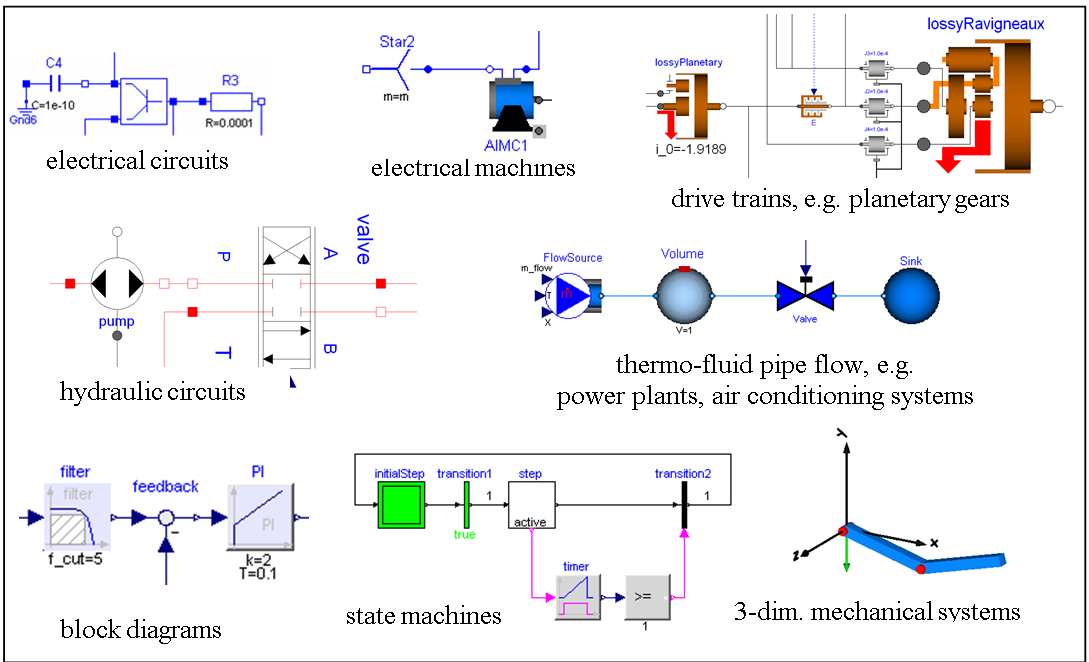
\includegraphics[width=5.92986in,height=3.59167in]{image2.png}

A schematic consists of connected components, like a resistor, or a
hydraulic cylinder. A component has ``connectors'' (often also called
``ports'') that describe the interaction possibilities, e.g., an
electrical pin, a mechanical flange, or an input signal. By drawing
connection lines between connectors a physical system or block diagram
model is constructed. Internally a component is defined by another
schematic or on ``bottom'' level, by an equation based description of
the model in Modelica syntax.

The Modelica language is a textual description to define all parts of a
model and to structure model components in libraries, called packages.
An appropriate Modelica simulation environment is needed to graphically
edit and browse a Modelica model (by interpreting the information
defining a Modelica model) and to perform model simulations and other
analysis. Information about such environments is available at
\href{http://www.modelica.org/tools}{www.modelica.org/tools}. Basically,
all Modelica language elements are mapped to differential, algebraic and
discrete equations. There are no language elements to describe directly
partial differential equations, although some types of discretized
partial differential equations can be reasonably defined, e.g., based on
the finite volume method and there are Modelica libraries to import
results of finite-element programs.

This document defines the details of the Modelica language. It is not
intended to learn the Modelica language with this text. There are better
alternatives, such as the Modelica books referenced at
\href{http://www.modelica.org/publications}{www.modelica.org/publications}.
This specification is used by computer scientist to implement a Modelica
translator and by modelers who want to understand the exact details of a
particular language element.

The Modelica language has been developed since 1996. This document
describes version 3.4 of the Modelica language. A complete summary is
available in \ref{modelica-3-4}.

% Introduction
\chapter{Introduction}\label{introduction1}

\section{Overview of Modelica}\label{overview-of-modelica}

Modelica is a language for modeling of physical systems, designed to
support effective library development and model exchange. It is a modern
language built on acausal modeling with mathematical equations and
object-oriented constructs to facilitate reuse of modeling knowledge.

\section{Scope of the Specification}\label{scope-of-the-specification}

The semantics of the Modelica language is specified by means of a set of
rules for translating any class described in the Modelica language to a
flat Modelica structure.
The semantic specification should be read together with the Modelica grammar.

A class (of specialized class \lstinline!model!, \lstinline!class! or \lstinline!block!) intended to be simulated on its own is called a \firstuse{simulation model}.

The flat Modelica structure is also defined for other cases than
simulation models; including functions (can be used to provide
algorithmic contents), packages (used as a structuring mechanism), and
partial models (used as base-models). This allows correctness to be
verified for those classes, before using them to build the simulation
model.

There are specific semantic restrictions for a simulation model to
ensure that the model is complete; they allow its flat Modelica
structure to be further transformed into a set of differential,
algebraic and discrete equations (= flat hybrid DAE). Note that
satisfying the semantic restrictions does not guarantee that the model
can be initialized from the initial conditions and simulated.

Modelica was designed to facilitate symbolic transformations of models, especially by mapping basically every Modelica language construct to equations in the flat Modelica structure.
Many Modelica models, especially in the associated Modelica Standard Library, are higher index systems, and can only be reasonably simulated if symbolic index reduction is performed, i.e., equations are differentiated and appropriate variables are selected as states, so that the resulting system of equations can be transformed to state space form (at least locally numerically), i.e., a hybrid DAE of index zero.
In order to allow this structural analysis, a tool may reject simulating a model if parameters cannot be evaluated during translation -- due to calls of external functions or initial equations/initial algorithms for \lstinline!fixed = false! parameters.
Accepting such models is a quality of implementation issue.
The Modelica specification does not define how to simulate a model.
However, it defines a set of equations that the simulation result should satisfy as well as possible.

The key issues of the translation (or flattening) are:
\begin{itemize}
\item
  Expansion of inherited base classes
\item
  Parameterization of base classes, local classes and components
\item
  Generation of connection equations from \lstinline!connect!-equations
\end{itemize}

The flat hybrid DAE form consists of:
\begin{itemize}
\item
  Declarations of variables with the appropriate basic types, prefixes
  and attributes, such as \lstinline!parameter Real v=5!.
\item
  Equations from equation sections.
\item
  Function invocations where an invocation is treated as a set of
  equations which involves all input and all result variables (number of
  equations = number of basic result variables).
\item
  Algorithm sections where every section is treated as a set of
  equations which involves the variables occurring in the algorithm
  section (number of equations = number of different assigned
  variables).
\item
  The \lstinline!when!-clauses where every \lstinline!when!-clause is treated as a set of conditionally evaluated equations, which are functions of the variables occurring in the clause (number of equations = number of different assigned variables).
\end{itemize}

Therefore, a flat hybrid DAE is seen as a set of equations where some of the equations are only conditionally evaluated.
Initial setup of the model is specified using \lstinline!start!-attributes and equations that hold only during initialization.

A Modelica class may also contain annotations, i.e.\ formal comments,
which specify graphical representations of the class (icon and diagram),
documentation text for the class, and version information.

\section{Some Definitions}\label{some-definitions}

Explanations of many terms can be found using the document index in \cref{document-index}.
Some important terms are defined below.

\begin{definition}[Component]\index{component}
An element defined by the production \lstinline[language=grammar]!component-clause! in the Modelica grammar (basically a variable or an instance of a class)
\end{definition}

\begin{definition}[Element]\index{element}
Class definition, \lstinline!extends!-clause, or \lstinline[language=grammar]!component-clause! declared in a class (basically a class reference or a component in a declaration).
\end{definition}

\begin{definition}[Flattening]\index{flattening}
The translation of a model described in Modelica to the corresponding model described as a hybrid DAE, involving expansion of inherited base classes, parameterization of base classes, local classes
and components, and generation of connection equations from \lstinline!connect!-equations (basically, mapping the hierarchical structure of a model into a set of differential, algebraic and discrete equations together with the corresponding variable declarations and function definitions from the model).
\end{definition}

% More terms that would be useful to define here:
% - translation (for phrases such as "during translation")
% - deprecated
% - quality of implementation
% - simulator

\section{Notation}\label{notation}

The remainder of this section shows examples of the presentation used in this document.

Syntax highlighting of Modelica code is illustrated by the code listing below.
Things to note include keywords that define code structure such as \lstinline!equation!, keywords that do not define code structure such as \lstinline!connect!, and recognized identifiers with meaning defined by the specification such as \lstinline!semiLinear!:
\begin{lstlisting}[language=modelica]
model Example "Example used to illustrate syntax highlighting"
  /* The string above is a class description string, this is a comment. */
  /* Invalid code is typically presented like this: */
  String s = 1.0; // Error: No conversion form Real to String.
  Real x;
equation
  2 * x = semiLinear(time - 0.5, 2, 3);
  /* The annotation below has omitted details represented by an ellipsis: */
  connect(resistor.n, conductor.p) annotation($\ldots$);
end Example;
\end{lstlisting}

Relying on implicit conversion of \lstinline!Integer! literals to \lstinline!Real! is common, as seen in the equation above (note use of Modelica code appearing inline in the text).

It is common to mix Modelica code with mathematical notation.
For example, \lstinline!average($x$, $y$)! could be defined as $\frac{x + y}{2}$.

\begin{definition}[Something]% Do not add this one to the index!
Text defining the meaning of \emph{something}.
\end{definition}

In addition to the style of definition above, new terminology can be introduced in the running text.
% TODO: Switch to \firstuse[---]{dummy} below.  For now, using \willintroduce to avoid risk of accidentally
% creating index entry in the future.
For example, a \willintroduce{dummy} is something that\ldots

\begin{nonnormative}
This is non-normative content that provides some explanation, motivation, and/or additional things to keep in mind.
It has no defining power and may be skipped by readers strictly interested in just the definition of the Modelica language.
\end{nonnormative}

\begin{example}
This is an example, which is a special kind of non-normative content.
Examples often contain a mix of code listings and explanatory text, and this is no exception:
\begin{lstlisting}[language=modelica]
String s = 1.0; // Error: No conversion form Real to String.
\end{lstlisting}
To fix the type mismatch above, the number has to be replaced by a \lstinline!String! expression, such as \lstinline!"1.0"!.
\end{example}

Other code listings in the document include specification of lexical units and grammatical structure, both using metasymbols of the extended BNF-grammar defined in~\cref{lexical-conventions}.
Lexical units are named with all upper-case letters and introduced with the `\lstinline[language=grammar]!=!' sign:
\begin{lstlisting}[language=grammar]
SOME-TOKEN = NON-DIGIT { DIGIT | NON-DIGIT }
\end{lstlisting}
Grammatical structure is recognized by production rules being named with lower-case letters and introduced with the `\lstinline[language=grammar]!:!' sign (also note appearance of the Modelica keyword \lstinline!der!):
\begin{lstlisting}[language=grammar]
differentiated-expression :
    der "(" SOME-TOKEN ")"
    | "(" differentiated-expression "+" differentiated-expression ")"
\end{lstlisting}


% Lexical Structure
\chapter{Lexical Structure}\label{lexical-structure}

This chapter describes several of the basic building blocks of Modelica
such as characters and lexical units including identifiers and literals.
Without question, the smallest building blocks in Modelica are single
characters belonging to a character set. Characters are combined to form
lexical units, also called tokens. These tokens are detected by the
lexical analysis part of the Modelica translator. Examples of tokens are
literal constants, identifiers, and operators. Comments are not really
lexical units since they are eventually discarded. On the other hand,
comments are detected by the lexical analyzer before being thrown away.

The information presented here is derived from the more formal
specification in \cref{modelica-concrete-syntax}.

\section{Character Set}\label{character-set}

The character set of the Modelica language is Unicode, but restricted to
the Unicode characters corresponding to 7-bit ASCII characters in
several places; for details see \cref{lexical-conventions}.

\section{Comments}\label{comments}

There are two kinds of comments in Modelica which are not lexical units
in the language and therefore are treated as white-space by a Modelica
translator. The white-space characters are space, tabulator, and line
separators (carriage return and line feed); and white-space cannot occur
inside tokens, e.g., \textless{}= must be written as two characters
without space or comments between them.  The following comment variants are
available:
%TODO-FORMAT should be a table instead of lstlisting?
\begin{lstlisting}[language=modelica]
// comment & Characters from // to the end of the line are ignored.
/* comment */ & Characters between /* and */ are ignored, including line terminators.
\end{lstlisting}

\begin{nonnormative}
The comment syntax is identical to that of C++.
\end{nonnormative}

Modelica comments do not nest, i.e., /* */ cannot be embedded within /*
*/. The following is \emph{invalid}:
\begin{lstlisting}[language=modelica]
/* Commented out - erroneous comment, invalid nesting of comments!
  /* This is an interesting model */
  model interesting
  ...
  end interesting;
*/
\end{lstlisting}

There is also a description-string, that is part of the Modelica language and
therefore not ignored by the Modelica translator. Such a description-string may
occur at the end of a declaration, equation, or statement or at the
beginning of a class definition. For example:
\begin{lstlisting}[language=modelica]
model TempResistor "Temperature dependent resistor"
  ...
  parameter Real R "Resistance for reference temp.";
  ...
end TempResistor;
\end{lstlisting}

\section{Identifiers, Names, and Keywords}\label{identifiers-names-and-keywords}

\willintroduce{Identifiers} are sequences of letters, digits, and other characters such as underscore, which are used for \emph{naming} various items in the language.
Certain combinations of letters are \willintroduce{keywords} represented as \emph{reserved} words in the Modelica grammar and are therefore not available as identifiers.

\subsection{Identifiers}\label{identifiers}

Modelica \firstuse{identifiers}\index{identifier}, used for naming classes, variables, constants, and other items, are of two forms.
The first form always starts with a letter or underscore (`\_'), followed by any number of letters, digits, or underscores.
Case is significant, i.e., the identifiers \lstinline!Inductor! and \lstinline!inductor! are different.
The second form \lstinline!(Q-IDENT)! starts with a single quote, followed by a sequence of any printable ASCII character, where single-quote must be preceded by backslash, and terminated by a single quote, e.g.\ \lstinline!'12H'!, \lstinline!'13\'H'!, \lstinline!'+foo'!.
Control characters in quoted identifiers have to use string escapes.
The single quotes are part of the identifier, i.e., \lstinline!'x'! and \lstinline!x! are distinct identifiers.
The redundant escapes (\lstinline!'\?'! and \lstinline!'\"'!) are the same as the corresponding non-escaped variants (\lstinline!'?'! and \lstinline!'"'!), but are only for use in Modelica source code.
A full BNF definition of the Modelica syntax and lexical units is available in \cref{modelica-concrete-syntax}.

\begin{lstlisting}[language=grammar,mathescape=false]
IDENT   = NONDIGIT { DIGIT | NONDIGIT } | Q-IDENT
Q-IDENT = "'" { Q-CHAR | S-ESCAPE } "'"
NONDIGIT = "_" | letters "a" ... "z" | letters "A" ... "Z"
DIGIT    = 0 | 1 | 2 | 3 | 4 | 5 | 6 | 7 | 8 | 9
Q-CHAR = NONDIGIT | DIGIT | "!" | "#" | "$" | "%" | "&" | "(" | ")" | "*" | "+" | "," | "-" | "." | "/" | ":" | ";" | "<" | ">" | "=" | "?" | "@" | "[" | "]" | "^" | "{" | "}"  | "|" | "~" | " " | """
S-ESCAPE = "\'" | "\"" | "\?" | "\\" | "\a" | "\b" | "\f" | "\n" | "\r" | "\t" | "\v"
\end{lstlisting}

\subsection{Names}\label{names}

A \firstuse{name}\index{name} is an identifier with a certain interpretation or meaning.
For example, a name may denote an \lstinline!Integer! variable, a \lstinline!Real! variable, a function, a type, etc.
A name may have different meanings in different parts of the code, i.e., different scopes.
The interpretation of identifiers as names is described in more detail in \cref{scoping-name-lookup-and-flattening}.
The meaning of package names is described in more detail in \cref{packages}.

\begin{example}
A name: \lstinline!Ele.Resistor!
\end{example}

A \firstuse{component reference}\index{component reference} is an expression containing a sequence of identifiers and indices.
A component reference is equivalent to the referenced object, which must be a component.
A component reference is resolved (evaluated) in the scope of a class (\cref{component-declarations}), or expression for the case of a local iterator variable (\cref{slice-operation}).

\begin{example}
A component reference: \lstinline!Ele.Resistor.u[21].r!
\end{example}

\subsection{Modelica Keywords}\label{modelica-keywords}

The following Modelica \firstuse{keywords}\index{keyword} are reserved words and shall not be used as identifiers, except as listed in \cref{lexical-conventions}:
\begin{center}
\begin{tabular}{l l l l l}
\lstinline!algorithm! & \lstinline!discrete! & \lstinline!false! & \lstinline!loop! & \lstinline!pure!\\ \hline
\lstinline!and! & \lstinline!each! & \lstinline!final! & \lstinline!model! & \lstinline!record!\\ \hline
\lstinline!annotation! & \lstinline!else! & \lstinline!flow! & \lstinline!not! & \lstinline!redeclare!\\ \hline
& \lstinline!elseif! & \lstinline!for! & \lstinline!operator! & \lstinline!replaceable!\\ \hline
\lstinline!block! & \lstinline!elsewhen! & \lstinline!function! & \lstinline!or! & \lstinline!return!\\ \hline
\lstinline!break! & \lstinline!encapsulated! & \lstinline!if! & \lstinline!outer! & \lstinline!stream!\\ \hline
\lstinline!class! & \lstinline!end! & \lstinline!import! & \lstinline!output! & \lstinline!then!\\ \hline
\lstinline!connect! & \lstinline!enumeration! & \lstinline!impure! & \lstinline!package! & \lstinline!true!\\ \hline
\lstinline!connector! & \lstinline!equation! & \lstinline!in! & \lstinline!parameter! & \lstinline!type!\\ \hline
\lstinline!constant! & \lstinline!expandable! & \lstinline!initial! & \lstinline!partial! & \lstinline!when!\\ \hline
\lstinline!constrainedby! & \lstinline!extends! & \lstinline!inner! & \lstinline!protected! & \lstinline!while!\\ \hline
\lstinline!der! & \lstinline!external! & \lstinline!input! & \lstinline!public! & \lstinline!within!\\
\end{tabular}
\end{center}

\section{Literal Constants}\label{literal-constants}

\firstuse{Literals}\index{literal} (or \emph{literal constants}) are unnamed constants used to build expressions, and have different forms depending on their type.
Each of the predefined types in Modelica has a way of expressing unnamed constants of the corresponding type, which is presented in the ensuing subsections.
Additionally, array literals and record literals can be expressed.

\subsection{Floating Point Numbers}\label{floating-point-numbers}

A floating point number is expressed as a decimal number in the form of a sequence of decimal digits followed by a decimal point, followed by decimal digits, followed by an exponent indicated by \lstinline!E! or \lstinline!e! followed by a sign and one or more decimal digits.
The various parts can be omitted, see \lstinline[language=grammar]!UNSIGNED-REAL! in~\cref{lexical-conventions} for details and also the examples below.
The minimal recommended range is that of IEEE double precision floating point numbers, for which the largest representable positive number is $1.7976931348623157\times10^{308}$ and the smallest positive number is $2.2250738585072014\times 10^{-308}$.
For example, the following are floating point number literal constants:
\begin{lstlisting}[language=modelica]
22.5, 3.141592653589793, 1.2E-35
\end{lstlisting}

The same floating point number can be represented by different literals.
For example, all of the following literals denote the same number:
\begin{lstlisting}[language=modelica]
13., 13E0, 1.3e1, 0.13E2, .13E2
\end{lstlisting}
The last variant shows that that the leading zero is optional (in that case decimal digits must be present).
Note that \lstinline!13! is not in this list, since it is not a floating point number,
but can be converted to a floating point number.

\subsection{Integer Literals}\label{integer-literals}

Literals of type \lstinline!Integer! are sequences of decimal digits, e.g.\ as in the integer numbers \lstinline!33!, \lstinline!0!, \lstinline!100!, \lstinline!30030044!.
The range of supported \lstinline!Integer! literals shall be at least large enough to represent the largest positive \lstinline!IntegerType! value, see \cref{integer-type}.

\begin{nonnormative}
Negative numbers are formed by unary minus followed by an integer literal.
\end{nonnormative}

\subsection{Boolean Literals}\label{boolean-literals}

The two \lstinline!Boolean! literal values are \lstinline!true!\indexinline{true} and \lstinline!false!\indexinline{false}.

\subsection{Strings}\label{strings}

String literals appear between double quotes as in \lstinline!"between"!.
Any character in the Modelica language character set (see \cref{lexical-conventions} for allowed characters) apart from double quote (\lstinline!"!) and backslash (\lstinline!\!), including new-line, can be \emph{directly} included in a string without using an escape sequence.
Certain characters in string literals can be represented using escape sequences\index{escape sequence!string literal}, i.e., the character is preceded by a backslash (\lstinline!\!) within the string.
Those characters are:
\begin{center}
\begin{tabular}{c l}
\hline
\tablehead{Character} & \tablehead{Description}\\
\hline
\hline
\lstinline!\'! & Single quote, may also appear without backslash in string constants\\
\lstinline!\"! & Double quote\\
\lstinline!\?! & Question-mark, may also appear without backslash in string constants\\
\lstinline!\\! & Backslash itself\\
\lstinline!\a! & Alert (bell, code 7, ctrl-G)\\
\lstinline!\b! & Backspace (code 8, ctrl-H)\\
\lstinline!\f! & Form feed (code 12, ctrl-L)\\
\lstinline!\n! & Newline (code 10, ctrl-J), same as literal newline\\
\lstinline!\r! & Carriage return (code 13, ctrl-M)\\
\lstinline!\t! & Horizontal tab (code 9, ctrl-I)\\
\lstinline!\v! & Vertical tab (code 11, ctrl-K)\\
\hline
\end{tabular}
\end{center}

For example, a string literal containing a tab, the words: \emph{This is},
double quote, space, the word: \emph{between}, double quote, space, the word:
\emph{us}, and new-line, would appear as follows:
\begin{lstlisting}[language=modelica]
"\tThis is\" between\" us\n"
\end{lstlisting}

Concatenation of string literals in certain situations (see the Modelica
grammar) is denoted by the + operator in Modelica, e.g.\ \lstinline!"a"! + \lstinline!"b"!
becomes \lstinline!"ab"!. This is useful for expressing long string literals that
need to be written on several lines.

The \lstinline!"\n"! character is used to conceptually indicate the
end of a line within a Modelica string. Any Modelica program that needs
to recognize line endings can check for a single \lstinline!"\n"!
character to do so on any platform. It is the responsibility of a
Modelica implementation to make any necessary transformations to other
representations when writing to or reading from a text file.

\begin{nonnormative}
For example, a \lstinline!"\n"! is written and read as-is in a Unix or Linux implementation, but written as
\lstinline!"\r\n"! pair, and converted back to \lstinline!"\n"! when read in a Windows implementation.
\end{nonnormative}

\begin{nonnormative}
For long string comments, e.g., the \lstinline!info! annotation to
store the documentation of a model, it would be very inconvenient, if
the string concatenation operator would have to be used for every line
of documentation. It is assumed that a Modelica tool supports the
non-printable newline character when browsing or editing a string
literal. For example, the following statement defines one string that
contains (non-printable) newline characters:
\begin{lstlisting}[language=modelica]
assert(noEvent(length > s_small),
"The distance between the origin of frame_a and the origin of frame_b
of a LineForceWithMass component became smaller as parameter s_small
(= a small number, defined in the
\"Advanced\" menu). The distance is
set to s_small, although it is smaller, to avoid a division by zero
when computing the direction of the line force.",
       level = AssertionLevel.warning);
\end{lstlisting}
\end{nonnormative}

\section{Operator Symbols}\label{operator-symbols}

The predefined operator symbols are formally defined on page \pageref{lexical-conventions} and
summarized in the table of operators in \cref{operator-precedence-and-associativity}.


% Operators and Expressions
\chapter{Operators and Expressions}\label{operators-and-expressions}

The lexical units are combined to form even larger building blocks such as \firstuse{expressions}\index{expression} according to the rules given by the \lstinline[language=grammar]!expression! part of the Modelica grammar in \cref{modelica-concrete-syntax}.
For example, they can be built from operators, function references, components, or component references (referring to components) and literals.
Each expression has a type and a variability.

This chapter describes the evaluation rules for expressions, the concept
of expression variability, built-in mathematical operators and
functions, and the built-in special Modelica operators with function
syntax.

Expressions can contain variables and constants, which have types,
predefined or user defined. The predefined built-in types of Modelica
are \lstinline!Real!, \lstinline!Integer!, \lstinline!Boolean!, \lstinline!String!, and enumeration types which are
presented in more detail in \cref{predefined-types-and-classes}.

\section{Expressions}\label{expressions}

Modelica equations, assignments and declaration equations contain
expressions.

Expressions can contain basic operations, \lstinline!+!, \lstinline!-!, \lstinline!*!, \lstinline!/!, \lstinline!^!, etc.\ with
normal precedence as defined in the Table in \cref{operator-precedence-and-associativity} and the grammar
in \cref{modelica-concrete-syntax}. The semantics of the operations is defined for both
scalar and array arguments in \cref{scalar-vector-matrix-and-array-operator-functions}.

It is also possible to define functions and call them in a normal
fashion. The function call syntax for both positional and named
arguments is described in \cref{positional-or-named-input-arguments-of-functions} and for vectorized calls in
\cref{initialization-and-binding-equations-of-components-in-functions}. The built-in array functions are given in \cref{array-dimension-lower-and-upper-index-bounds}
and other built-in operators in \cref{built-in-intrinsic-operators-with-function-syntax}.

\section{Operator Precedence and Associativity}\label{operator-precedence-and-associativity}

Operator precedence determines the order of evaluation of operators in
an expression. An operator with higher precedence is evaluated before an
operator with lower precedence in the same expression.

The following table presents all the expression operators in order of precedence.
\begin{table}[H]
% Beware that the array construction operator, normally expressed as \lstinline!{ }! needs escaped braces inside \caption.
% This isn't handled correctly by LaTeXML, as reported here:
% - https://github.com/brucemiller/LaTeXML/issues/1377
\caption{Operators in order of precedence from highest to lowest, as derived from the Modelica grammar in \cref{modelica-concrete-syntax}.  All operators are binary except the postfix operators and those shown as unary together with \emph{expr}, the conditional operator, the array construction operator \lstinline!\{ \}! and concatenation operator \lstinline![ ]!, and the array range constructor which is either binary or ternary.  Operators with the same precedence occur at the same table row.}\label{tab:operator-precedence}
\begin{center}
\begin{tabular}{l l l}
\hline
\tablehead{Operator group} & \tablehead{Operator syntax} & \tablehead{Examples}\\
\hline
\hline
Postfix array index operator & \lstinline![]! & \lstinline!arr[index]!\\
\hline
Postfix access operator & \lstinline!.! & \lstinline!a.b!\\
\hline
Postfix function call & \lstinline!$\mathit{funcName}$($\mathit{functionArguments}$)! & \lstinline!sin(4.36)!\\
\hline
Array construction & \lstinline!{$\mathit{expressions}$}! & \lstinline!{2, 3}!\\
Horizontal concatenation & \lstinline![$\mathit{expressions}$]! & \lstinline![5, 6]!\\
Vertical concatenation & \lstinline![$\mathit{expressions}$; $\mathit{expressions}\ldots$]! & \lstinline![2, 3; 7, 8]!\\
\hline
Exponentiation & \ \lstinline!^! & \lstinline!2 ^ 3!\\
\hline
Multiplicative  & \lstinline!* /! & \lstinline!2 * 3!, \lstinline!2 / 3!\\
Elementwise multiplicative & \lstinline!.* ./! & \lstinline![1, 2; 3, 4] .* [2, 3; 5, 6]!\\
\hline
Additive & \lstinline!+ -! & \lstinline!1 + 2!\\
Additive unary & \lstinline!+$\mathit{expr}$ -$\mathit{expr}$! & \lstinline!-0.5!\\
Array elementwise additive & \lstinline!.+ .-! & \lstinline![1, 2; 3, 4] .+ [2, 3; 5, 6]!\\
\hline
Relational & \lstinline!< <= > >= == <>! & \lstinline!a < b!, \lstinline!a <= b!, \lstinline!a > b!, \ldots\\
\hline
Unary negation & \lstinline!not $\mathit{expr}$! & \lstinline!not b1!\\
\hline
Logical and & \lstinline!and! & \lstinline!b1 and b2!\\
\hline
Logical or & \lstinline!or! & \lstinline!b1 or b2!\\
\hline
\multirow{2}{*}{Array range} & \lstinline!$\mathit{expr}$ : $\mathit{expr}$! & \lstinline!1 : 5!\\
                             & \lstinline!$\mathit{expr}$ : $\mathit{expr}$ : $\mathit{expr}$! & \lstinline!start : step : stop!\\
\hline
Conditional & \lstinline!if $\mathit{expr}$ then $\mathit{expr}$ else $\mathit{expr}$! & \lstinline!if b then 3 else x!\\
\hline
Named argument & \lstinline!$\mathit{ident}$ = $\mathit{expr}$! & \lstinline!x = 2.26!\\
\hline
\end{tabular}
\end{center}
\end{table}

The conditional operator may also include \lstinline!elseif!-branches.
Equality \lstinline!=! and assignment \lstinline!:=! are not expression operators since they are allowed only in equations and in assignment statements respectively.
All binary expression operators are left associative, except exponentiation which is non-associative.
The array range operator is non-associative.

\begin{nonnormative}
The unary minus and plus in Modelica is slightly different than in Mathematica\footnote{\emph{Mathematica} is a registered trademark of Wolfram Research Inc.} and in MATLAB\footnote{\emph{MATLAB} is
a registered trademark of MathWorks Inc.}, since the following expressions are illegal (whereas in Mathematica and in MATLAB these are valid expressions):
\begin{lstlisting}[language=modelica]
2*-2  // = -4 in Mathematica/MATLAB; is illegal in Modelica
--2   // = 2 in Mathematica/MATLAB; is illegal in Modelica
++2   // = 2 in Mathematica/MATLAB; is illegal in Modelica
2--2  // = 4 in Mathematica/MATLAB; is illegal in Modelica
\end{lstlisting}

Non-associative exponentiation and array range operator:
\begin{lstlisting}[language=modelica]
x^y^z         // Not legal, use parenthesis to make it clear
a:b:c:d:e:f:g // Not legal, and scalar arguments gives no legal interpretation.
\end{lstlisting}
\end{nonnormative}

\section{Evaluation Order}\label{evaluation-order}

A tool is free to solve equations, reorder expressions and to not evaluate expressions if their values do not influence the result (e.g.\ short-circuit evaluation of \lstinline!Boolean! expressions).
\lstinline!if!-statements and \lstinline!if!-expressions guarantee that their branches are only evaluated if the appropriate condition is true, but relational operators generating state or time events will during continuous integration have the value from the most recent event.

If a numeric operation overflows the result is undefined. For literals
it is recommended to automatically convert the number to another type
with greater precision.

\subsection{Example: Guarding Expressions Against Incorrect Evaluation}\label{example-guarding-expressions-against-incorrect-evaluation}

\begin{example}
If one wants to guard an expression against incorrect evaluation, it should be guarded by an \lstinline!if!:
\begin{lstlisting}[language=modelica]
  Boolean v[n];
  Boolean b;
  Integer I;
equation
  b=(I>=1 and I<=n) and v[I]; // Invalid
  b=if (I>=1 and I<=n) then v[I] else false; // Correct
\end{lstlisting}

To guard square against square root of negative number use \lstinline!noEvent!:
\begin{lstlisting}[language=modelica]
der(h)=if h>0 then -c*sqrt(h) else 0; // Incorrect
der(h)=if noEvent(h>0) then -c*sqrt(h) else 0; // Correct
\end{lstlisting}
\end{example}

\section{Arithmetic Operators}\label{arithmetic-operators}

Modelica supports five binary arithmetic operators that operate on any numerical type:
\begin{center}
\begin{tabular}{c|l}
\tablehead{Operator} & \tablehead{Description} \\
\hline
\hline
\lstinline!^! & Exponentiation\\
\lstinline!*! & Multiplication\\
\lstinline!/! & Division\\
\lstinline!+! & Addition\\
\lstinline!-! & Subtraction\\
\hline
\end{tabular}
\end{center}

Some of these operators can also be applied to a combination of a scalar
type and an array type, see \cref{scalar-vector-matrix-and-array-operator-functions}.

The syntax of these operators is defined by the following rules from the
Modelica grammar:
\begin{lstlisting}[language=grammar]
arithmetic-expression :
   [ add-operator ] term { add-operator term }

add-operator :
   "+" | "-"

term :
   factor { mul-operator factor }

mul-operator :
   "*" | "/"

factor :
   primary [ "^" primary ]
\end{lstlisting}

\section{Equality, Relational, and Logical Operators}\label{equality-relational-and-logical-operators}

Modelica supports the standard set of relational and logical operators, all of which produce the standard boolean values \lstinline!true! or \lstinline!false!:
\begin{center}
\begin{tabular}{c|l}
\tablehead{Operator} & \tablehead{Description} \\
\hline
\hline
\lstinline!>! & Greater than\\
\lstinline!>=! & Greater than or equal\\
\lstinline!<! & Less than\\
\lstinline!<=! & Less than or equal to\\
\lstinline!==! & Equality within expressions\\
\lstinline!<>! & Inequality\\
\hline
\end{tabular}
\end{center}

A single equals sign \lstinline!=! is never used in relational expressions, only in
equations (\cref{equations}, \cref{equality-and-assignment}) and in function calls using named
parameter passing (\cref{positional-or-named-input-arguments-of-functions}).

The following logical operators are defined:
\begin{center}
\begin{tabular}{c|l}
\tablehead{Operator} & \tablehead{Description} \\
\hline
\hline
\lstinline!not!\indexinline{not} & Logical negation (unary operator)\\
\lstinline!and!\indexinline{and} & Logical \emph{and} (conjunction)\\
\lstinline!or!\indexinline{or} & Logical \emph{or} (disjunction)\\
\hline
\end{tabular}
\end{center}

The grammar rules define the syntax of the relational and logical operators.
\begin{lstlisting}[language=grammar]
logical-expression :
   logical-term { or logical-term }

logical-term :
   logical-factor { and logical-factor }

logical-factor :
   [ not ] relation

relation :
   arithmetic-expression [ relational-operator arithmetic-expression ]

relational-operator :
   "<" | "<=" | ">" | ">=" | "==" | "<>"
\end{lstlisting}

The following holds for relational operators:
\begin{itemize}
\item
  Relational operators \lstinline!<!, \lstinline!<=!,\lstinline!>!,
\lstinline!>=!, \lstinline!==!, \lstinline!<>!, are only defined for
  scalar operands of simple types. The result is \lstinline!Boolean! and is true or
  false if the relation is fulfilled or not, respectively.
\item
  For operands of type \lstinline!String!, \lstinline!str1 $\mathit{op}$ str2! is for each relational
  operator, $\mathit{op}$, defined in terms of the C function \lstinline[language=C]!strcmp! as
  \lstinline[language=C]!strcmp(str1, str2) $\mathit{op}$ 0!.
\item
  For operands of type \lstinline!Boolean!, \lstinline!false < true!.
\item
  For operands of enumeration types, the order is given by the order of
  declaration of the enumeration literals.
\item
  In relations of the form \lstinline!v1 == v2 or v1 <> v2!,
  \lstinline!v1! or \lstinline!v2! shall, unless used in a function, not be a subtype of \lstinline!Real!.
  \begin{nonnormative}
  The reason for this rule is that relations with \lstinline!Real! arguments are transformed to state events (see Events, \cref{events-and-synchronization}) and this transformation becomes unnecessarily complicated for the \lstinline!==! and \lstinline!<>! relational operators (e.g.\ two crossing functions instead of one crossing function needed, epsilon strategy needed even at event instants).  Furthermore, testing on equality of \lstinline!Real! variables is questionable on machines where the number length in registers is different to number length in main memory.
  \end{nonnormative}
\item
  Relational operators can generate events, see \cref{discrete-time-expressions}.
\end{itemize}

\section{Miscellaneous Operators and Variables}\label{miscellaneous-operators-and-variables}

Modelica also contains a few built-in operators which are not standard
arithmetic, relational, or logical operators. These are described below,
including \lstinline!time!, which is a built-in variable, not an operator.

\subsection{String Concatenation}\label{string-concatenation}

Concatenation of strings (see the Modelica grammar) is denoted by the \lstinline!+!
operator in Modelica.

\begin{example}
\lstinline!"a" + "b"! becomes \lstinline!"ab"!.
\end{example}

\subsection{Array Constructor Operator}\label{array-constructor-operator}

The array constructor operator \lstinline!{ $\ldots$ }! is described in \cref{vector-matrix-and-array-constructors}.

\subsection{Array Concatenation Operator}\label{array-concatenation-operator}

The array concatenation operator \lstinline![ $\ldots$ ]! is described in \cref{array-concatenation}.

\subsection{Array Range Operator}\label{array-range-operator}

The array range constructor operator \lstinline!:! is described in \cref{vector-construction}.

\subsection{If-Expressions}\label{if-expressions}

An expression
\begin{lstlisting}[language=modelica]
if expression1 then expression2 else expression3
\end{lstlisting}%
\index{if@\robustinline{if}!expression}\index{then@\robustinline{then}!if-expression@\robustinline{if}-expression}\index{else@\robustinline{else}!if-expression@\robustinline{if}-expression}
is one example of \lstinline!if!-expression. First \lstinline!expression1!, which must be \lstinline!Boolean! expression, is evaluated.
If \lstinline!expression1! is true \lstinline!expression2! is evaluated and is the value of the \lstinline!if!-expression, else \lstinline!expression3! is evaluated and is the value of the \lstinline!if!-expression.
The two expressions, \lstinline!expression2! and \lstinline!expression3!, must be type compatible expressions (\cref{type-compatible-expressions}) giving the type of the \lstinline!if!-expression.
The \lstinline!if!-expressions with \lstinline!elseif!\index{elseif@\robustinline{elseif}!if-expression} are defined by replacing \lstinline!elseif! by \lstinline!else if!.
For short-circuit evaluation see \cref{evaluation-order}.

\begin{nonnormative}
\lstinline!elseif! in expressions has been added to the Modelica language for symmetry with \lstinline!if!-equations.
\end{nonnormative}

\begin{example}
\begin{lstlisting}[language=modelica]
Integer i;
Integer sign_of_i1=if i<0 then -1 elseif i==0 then 0 else 1;
Integer sign_of_i2=if i<0 then -1 else if i==0 then 0 else 1;
\end{lstlisting}
\end{example}

\subsection{Member Access Operator}\label{member-access-operator}

It is possible to access members of a class instance using dot notation,
i.e., the \lstinline!.! operator.

\begin{example}
\lstinline!R1.R! for accessing the resistance component \lstinline!R!
of resistor \lstinline!R1!. Another use of dot notation: local classes
which are members of a class can of course also be accessed using dot
notation on the name of the class, not on instances of the class.
\end{example}

\subsection{Built-in Variable time}\label{built-in-variable-time}

All declared variables are functions of the independent variable \lstinline!time!.
The variable \lstinline!time! is a built-in variable available in all models and
blocks, which is treated as an input variable. It is implicitly defined
as:
\begin{lstlisting}[language=modelica]
input Real time (final quantity = "Time",
                 final unit = "s");
\end{lstlisting}

The value of the \lstinline!start!-attribute of \lstinline!time! is set to the time instant at which the simulation is started.

\begin{example}
\begin{lstlisting}[language=modelica]
encapsulated model SineSource
  import Modelica.Math.sin;
  connector OutPort = output Real;
  OutPort y = sin(time); // Uses the built-in variable time.
end SineSource;
\end{lstlisting}
\end{example}

\section{Built-in Intrinsic Operators with Function Syntax}\label{built-in-intrinsic-operators-with-function-syntax}

Certain built-in operators of Modelica have the same syntax as a
function call. However, they do not behave as a mathematical function,
because the result depends not only on the input arguments but also on
the status of the simulation.

There are also built-in functions that depend only on the input
argument, but also may trigger events in addition to returning a value.
Intrinsic means that they are defined at the Modelica language level,
not in the Modelica library. The following built-in intrinsic
operators/functions are available:
\begin{itemize}
\item
  Mathematical functions and conversion functions, see \cref{numeric-functions-and-conversion-functions}
  below.
\item
  Derivative and special purpose operators with function syntax, see
  \cref{derivative-and-special-purpose-operators-with-function-syntax} below.
\item
  Event-related operators with function syntax, see \cref{event-related-operators-with-function-syntax} below.
\item
  Array operators/functions, see \cref{array-dimension-lower-and-upper-index-bounds}.
\end{itemize}

Note that when the specification references a function having the name
of a built-in function it references the built-in function, not a
user-defined function having the same name, see also \cref{built-in-functions}. With
exception of the built-in \lstinline!String! operator, all operators in this section
can only be called with positional arguments.

\subsection{Numeric Functions and Conversion Functions}\label{numeric-functions-and-conversion-functions}

The mathematical functions and conversion operators are listed below do not generate events.
\begin{center}
\begin{tabular}{l|l l}
\hline
\tablehead{Expression} & \tablehead{Description} & \tablehead{Details}\\
\hline
\hline
\lstinline!abs($v$)! & Absolute value (event-free) & \Cref{modelica:abs} \\
\lstinline!sign($v$)! & Sign of argument (event-free) & \Cref{modelica:sign} \\
\lstinline!sqrt($v$)! & Square root & \Cref{modelica:sqrt} \\
\lstinline!Integer($e$)! & Conversion from enumeration to \lstinline!Integer! & \Cref{modelica:integer-of-enumeration} \\
\lstinline!EnumTypeName($i$)! & Conversion from \lstinline!Integer! to enumeration & \Cref{modelica:enumeration-of-integer} \\
\lstinline!String($\ldots$)! & Conversion to \lstinline!String! & \Cref{modelica:to-String} \\
\hline
\end{tabular}
\end{center}

All of these except for the \lstinline!String! conversion operator are vectorizable according to \cref{scalar-functions-applied-to-array-arguments}.

Additional non-event generating mathematical functions are described in \cref{built-in-mathematical-functions-and-external-built-in-functions}, whereas the event-triggering mathematical functions are described in \cref{event-triggering-mathematical-functions}.

\begin{functiondefinition}[abs]
\begin{synopsis}\begin{lstlisting}
abs($v$)
\end{lstlisting}\end{synopsis}
\begin{semantics}
Expands into \lstinline!noEvent(if $v$ >= 0 then $v$ else -$v$)!.  Argument $v$ needs to be an \lstinline!Integer! or \lstinline!Real! expression.
\end{semantics}
\end{functiondefinition}

\begin{functiondefinition}[sign]
\begin{synopsis}\begin{lstlisting}
sign($v$)
\end{lstlisting}\end{synopsis}
\begin{semantics}
Expands into \lstinline!noEvent(if $v$ > 0 then 1 else if $v$ < 0 then -1 else 0)!.  Argument $v$ needs to be an \lstinline!Integer! or \lstinline!Real! expression.
\end{semantics}
\end{functiondefinition}

\begin{functiondefinition}[sqrt]
\begin{synopsis}\begin{lstlisting}
sqrt($v$)
\end{lstlisting}\end{synopsis}
\begin{semantics}
Square root of $v$ if $v \geq 0$, otherwise an error occurs.  Argument $v$ needs to be an \lstinline!Integer! or \lstinline!Real! expression.
\end{semantics}
\end{functiondefinition}

\begin{operatordefinition*}[Integer]\label{modelica:integer-of-enumeration}\index{Integer@\robustinline{Integer}!conversion operator}
\begin{synopsis}\begin{lstlisting}
Integer($e$)
\end{lstlisting}\end{synopsis}
\begin{semantics}
Ordinal number of the expression $e$ of enumeration type that evaluates to the enumeration value \lstinline!E.enumvalue!, where \lstinline!Integer(E.e1) = 1!, \lstinline!Integer(E.en) = n!, for an enumeration type \lstinline!E = enumeration(e1, $\ldots$, en)!.
See also \cref{type-conversion-of-enumeration-values-to-string-or-integer}.
\end{semantics}
\end{operatordefinition*}

\begin{operatordefinition*}[<EnumTypeName>]\label{modelica:enumeration-of-integer}\index{enumeration@\robustinline{enumeration}!conversion operator}
\begin{synopsis}\begin{lstlisting}
EnumTypeName($i$)
\end{lstlisting}\end{synopsis}
\begin{semantics}
For any enumeration type \lstinline!EnumTypeName!, returns the enumeration value \lstinline!EnumTypeName.e! such that $\text{\lstinline!Integer(EnumTypeName.e)!} = i$.  Refer to the definition of \lstinline!Integer! above.

It is an error to attempt to convert values of $i$ that do not correspond to values of the enumeration type.  See also \cref{type-conversion-of-integer-to-enumeration-values}.
\end{semantics}
\end{operatordefinition*}

\begin{operatordefinition*}[String]\label{modelica:to-String}\index{String@\robustinline{String}!conversion operator}
\begin{synopsis}\begin{lstlisting}
String($b$, <options>)
String($i$, <options>)
String($r$, significantDigits=$d$, <options>)
String($r$, format=$s$)
String($e$, <options>)
\end{lstlisting}\end{synopsis}
\begin{semantics}
Convert a scalar non-\lstinline!String! expression to a \lstinline!String! representation.  The first argument may be a \lstinline!Boolean! $b$, an \lstinline!Integer! $i$, a \lstinline!Real! $r$ or an enumeration value $e$ (\cref{type-conversion-of-enumeration-values-to-string-or-integer}).  The other arguments must use named arguments.  For \lstinline!Real! expressions the output shall be according to the Modelica grammar.

The optional \lstinline!<options>! are:
\begin{itemize}
\item
  \lstinline!Integer minimumLength = 0!: Minimum length of the resulting string.  If necessary, the blank character is used to fill up unused space.
\item
  \lstinline!Boolean leftJustified = true!: If true, the converted result is left justified in the string; if false it is right justified in the string.
\item
  \lstinline!Integer significantDigits = 6!: Number of significant digits in the result string.
\end{itemize}

\begin{nonnormative}
Examples of \lstinline!Real! values formatted with 6 significant digits: \emph{12.3456}, \emph{0.0123456}, \emph{12345600}, \emph{1.23456E-10}.
\end{nonnormative}

The \lstinline!format! string corresponding to \lstinline!<options>! is:
\begin{itemize}
\item
  For \lstinline!Real!:\\
  \lstinline!(if leftJustified then "-" else "") + String(minimumLength)!\\
  \lstinline!  + "." + String(signficantDigits) + "g"!
\item
  For \lstinline!Integer!:\\
  \lstinline!(if leftJustified then "-" else "") + String(minimumLength) + "d"!
\end{itemize}

Form of the \lstinline!format! string:  According to ANSI-C the format string specifies one conversion specifier (excluding the leading \%), shall not contain length modifiers, and shall not use `\lstinline!*!' for width and/or precision.  For all numeric values the format specifiers `\lstinline!f!', `\lstinline!e!', `\lstinline!E!', `\lstinline!g!', `\lstinline!G!' are allowed.  For integral values it is also allowed to use the `\lstinline!d!', `\lstinline!i!', `\lstinline!o!', `\lstinline!x!', `\lstinline!X!', `\lstinline!u!', and `\lstinline!c!' format specifiers (for non-integral values a tool may round, truncate or use a different format if the integer conversion characters are used).

The `\lstinline!x!'/`\lstinline!X!' formats (hexa-decimal) and \lstinline!c! (character) for \lstinline!Integer! values give results that do not agree with the Modelica grammar.
\end{semantics}
\end{operatordefinition*}


\subsection{Event Triggering Mathematical Functions}\label{event-triggering-mathematical-functions}

The operators listed below trigger events if used outside of a \lstinline!when!-clause and outside of a clocked discrete-time partition (see \cref{clocked-discrete-time-and-clocked-discretized-continuous-time-partition}).
\begin{center}
\begin{tabular}{l|l l}
\hline
\tablehead{Expression} & \tablehead{Description} & \tablehead{Details}\\
\hline
\hline
\lstinline!div($x$, $y$)! & Division with truncation toward zero & \Cref{modelica:div} \\
\lstinline!mod($x$, $y$)! & Integer modulus & \Cref{modelica:mod} \\
\lstinline!rem($x$, $y$)! & Integer remainder & \Cref{modelica:rem} \\
\lstinline!ceil($x$)! & Smallest integer \lstinline!Real! not less than $x$ & \Cref{modelica:ceil} \\
\lstinline!floor($x$)! & Largest integer \lstinline!Real! not greater than $x$ & \Cref{modelica:floor} \\
\lstinline!integer($x$)! & Largest \lstinline!Integer! not greater than $x$ & \Cref{modelica:integer} \\
\hline
\end{tabular}
\end{center}

These expression for \lstinline!div!, \lstinline!ceil!, \lstinline!floor!, and \lstinline!integer! are event generating expression.  The event generating expression for \lstinline!mod(x,y)! is \lstinline!floor(x/y)!, and for \lstinline!rem(x,y)! it is \lstinline!div(x,y)! -- i.e.\ events are not generated when \lstinline!mod! or \lstinline!rem! changes continuously in an interval, but when they change discontinuously from one interval to the next.

\begin{nonnormative}
If this is not desired, the \lstinline!noEvent! operator can be applied to them.  E.g.\ \lstinline!noEvent(integer(v))!.
\end{nonnormative}

\begin{operatordefinition}[div]
\begin{synopsis}\begin{lstlisting}
div($x$, $y$)
\end{lstlisting}\end{synopsis}
\begin{semantics}
Algebraic quotient $x / y$ with any fractional part discarded (also known as truncation toward zero).
\begin{nonnormative}
This is defined for \lstinline!/! in C99; in C89 the result for negative numbers is implementation-defined, so the standard function \lstinline[language=C]!div! must be used.
\end{nonnormative}
Result and arguments shall have type \lstinline!Real! or \lstinline!Integer!.  If either of the arguments is \lstinline!Real! the result is \lstinline!Real! otherwise \lstinline!Integer!.
\end{semantics}
\end{operatordefinition}

\begin{operatordefinition}[mod]
\begin{synopsis}\begin{lstlisting}
mod($x$, $y$)
\end{lstlisting}\end{synopsis}
\begin{semantics}
Integer modulus of $x / y$, i.e. \lstinline!mod($x$, $y$) = $x$ - floor($x$ / $y$) * $y$!.  Result and arguments shall have type \lstinline!Real! or \lstinline!Integer!.  If either of the arguments is \lstinline!Real! the result is \lstinline!Real! otherwise \lstinline!Integer!.
\begin{nonnormative}
Note, outside of a \lstinline!when!-clause state events are triggered when the return value changes discontinuously.  Examples: \lstinline!mod(3, 1.4) = 0.2!, \lstinline!mod(-3, 1.4) = 1.2!, \lstinline!mod(3, -1.4) = -1.2!.
\end{nonnormative}
\end{semantics}
\end{operatordefinition}

\begin{operatordefinition}[rem]
\begin{synopsis}\begin{lstlisting}
rem($x$, $y$)
\end{lstlisting}\end{synopsis}
\begin{semantics}
Integer remainder of $x / y$, such that \lstinline!div($x$, $y$) * $y$ + rem($x$, $y$) = $x$!.  Result and arguments shall have type \lstinline!Real! or \lstinline!Integer!.  If either of the arguments is \lstinline!Real! the result is \lstinline!Real! otherwise \lstinline!Integer!.
\begin{nonnormative}
Note, outside of a \lstinline!when!-clause state events are triggered when the return value changes discontinuously.  Examples: \lstinline!rem(3, 1.4) = 0.2!, \lstinline!rem(-3, 1.4) = -0.2!.
\end{nonnormative}
\end{semantics}
\end{operatordefinition}

\begin{operatordefinition}[ceil]
\begin{synopsis}\begin{lstlisting}
ceil($x$)
\end{lstlisting}\end{synopsis}
\begin{semantics}
Smallest integer not less than $x$.  Result and argument shall have type \lstinline!Real!.
\begin{nonnormative}
Note, outside of a \lstinline!when!-clause state events are triggered when the return value changes discontinuously.
\end{nonnormative}
\end{semantics}
\end{operatordefinition}

\begin{operatordefinition}[floor]
\begin{synopsis}\begin{lstlisting}
floor($x$)
\end{lstlisting}\end{synopsis}
\begin{semantics}
Largest integer not greater than $x$.  Result and argument shall have type \lstinline!Real!.
\begin{nonnormative}
Note, outside of a \lstinline!when!-clause state events are triggered when the return value changes discontinuously.
\end{nonnormative}
\end{semantics}
\end{operatordefinition}

\begin{operatordefinition}[integer]
\begin{synopsis}\begin{lstlisting}
integer($x$)
\end{lstlisting}\end{synopsis}
\begin{semantics}
Largest integer not greater than $x$.  The argument shall have type \lstinline!Real!.  The result has type \lstinline!Integer!.
\begin{nonnormative}
Note, outside of a \lstinline!when!-clause state events are triggered when the return value changes discontinuously.
\end{nonnormative}
\end{semantics}
\end{operatordefinition}

\subsection{Elementary Mathematical Functions}\label{built-in-mathematical-functions-and-external-built-in-functions}

The functions listed below are elementary mathematical functions.  Tools are expected to utilize well known properties of these functions (derivatives, inverses, etc) for symbolic processing of expressions and equations.
\begin{center}
\begin{tabular}{l|l l}
\hline
\tablehead{Expression} & \tablehead{Description} & \tablehead{Details}\\
\hline
\hline
\lstinline!sin($x$)!        \indexinline{sin}   & Sine & \\
\lstinline!cos($x$)!        \indexinline{cos}   & Cosine & \\
\lstinline!tan($x$)!        \indexinline{tan}   & Tangent ($x$ shall not be: $\ldots$, -$\pi/2$, $\pi/2$, $3\pi/2$, $\ldots$) & \\
\lstinline!asin($x$)!       \indexinline{asin}  & Inverse sine ($-1 \le x \le 1$) & \\
\lstinline!acos($x$)!       \indexinline{acos}  & Inverse cosine ($-1 \le x \le 1$) & \\
\lstinline!atan($x$)!       \indexinline{atan}  & Inverse tangent & \\
\lstinline!atan2($y$, $x$)! \indexinline{atan2} & Principal value of the arc tangent of $y/x$ & \Cref{modelica:atan2} \\
\lstinline!sinh($x$)!       \indexinline{sinh}  & Hyperbolic sine & \\
\lstinline!cosh($x$)!       \indexinline{cosh}  & Hyperbolic cosine & \\
\lstinline!tanh($x$)!       \indexinline{tanh}  & Hyperbolic tangent & \\
\lstinline!exp($x$)!        \indexinline{exp}   & Exponential, base $\mathrm{e}$ & \\
\lstinline!log($x$)!        \indexinline{log}   & Natural (base $\mathrm{e}$) logarithm ($x > 0$) & \\
\lstinline!log10($x$)!      \indexinline{log10} & Base 10 logarithm ($x > 0$) & \\
\hline
\end{tabular}
\end{center}

These functions are the only ones that can also be called using the deprecated \lstinline!"builtin"! external language, see \cref{external-function-interface}.

\begin{nonnormative}
End user oriented information about the elementary mathematical functions can be found for the corresponding functions in the \lstinline!Modelica.Math! package.
\end{nonnormative}

\begin{functiondefinition}[atan2]
\begin{synopsis}\begin{lstlisting}
atan2($y$, $x$)
\end{lstlisting}\end{synopsis}
\begin{semantics}
Principal value of the arc tangent of $y/x$, using the signs of the two arguments to determine the quadrant of the result.  The result $\varphi$ is in the interval $\left[-\pi,\, \pi\right]$ and satisfies:
\begin{equation*}
\begin{aligned}
\abs{(x,\, y)}\, \cos(\varphi) &= x\\
\abs{(x,\, y)}\, \sin(\varphi) &= y
\end{aligned}
\end{equation*}
\end{semantics}
\end{functiondefinition}

\subsection{Derivative and Special Purpose Operators with Function Syntax}\label{derivative-and-special-purpose-operators-with-function-syntax}

The operators listed below include the derivative operator and special purpose operators with function syntax.
\begin{center}
\begin{tabular}{l|l l}
\hline
\tablehead{Expression} & \tablehead{Description} & \tablehead{Details}\\
\hline
\hline
\lstinline!der($\mathit{expr}$)! & Time derivative & \Cref{modelica:der} \\
\lstinline!delay($\mathit{expr}$, $\ldots$)! & Time delay & \Cref{modelica:delay} \\
\lstinline!cardinality($c$)! & Number of occurrences in \lstinline!connect!-equations & \Cref{modelica:cardinality} \\
\lstinline!homotopy($\mathit{actual}$, $\mathit{simplified}$)! & Homotopy initialization & \Cref{modelica:homotopy} \\
\lstinline!semiLinear($x$, $k^{+}$, $k^{-}$)! & Sign-dependent slope & \Cref{modelica:semiLinear} \\
\lstinline!inStream($v$)! & Stream variable flow into component & \Cref{modelica:inStream} \\
\lstinline!actualStream($v$)! & Actual value of stream variable & \Cref{modelica:actualStream} \\
\lstinline!spatialDistribution($\ldots$)! & Variable-speed transport & \Cref{modelica:spatialDistribution} \\
\lstinline!getInstanceName()! & Name of instance at call site & \Cref{modelica:getInstanceName} \\
\hline
\end{tabular}
\end{center}

The special purpose operators with function syntax where the call below uses named arguments can be called with named arguments (with the specified names), or with positional arguments (the inputs of the functions are in the order given in the calls below).

\begin{operatordefinition}[der]
\begin{synopsis}\begin{lstlisting}
der($\mathit{expr}$)
\end{lstlisting}\end{synopsis}
\begin{semantics}
The time derivative of $\mathit{expr}$.
If the expression $\mathit{expr}$ is a scalar it needs to be a subtype of \lstinline!Real!.
The expression and all its time-varying subexpressions must be continuous and semi-differentiable.
If $\mathit{expr}$ is an array, the operator is applied to all elements of the array.
For non-scalar arguments the function is vectorized according to \cref{vectorized-calls-of-functions}.
\begin{nonnormative}
For \lstinline!Real! parameters and constants the result is a zero scalar or array of the same size as the variable.
\end{nonnormative}
\end{semantics}
\end{operatordefinition}

\begin{operatordefinition}[delay]
\begin{synopsis}\begin{lstlisting}
delay($\mathit{expr}$, $\mathit{delayTime}$, $\mathit{delayMax}$)
delay($\mathit{expr}$, $\mathit{delayTime}$)
\end{lstlisting}\end{synopsis}
\begin{semantics}
Evaluates to \lstinline!$\mathit{expr}$(time - $\mathit{delayTime}$)! for $\text{\lstinline!time!} > \text{\lstinline!time.start!} + \mathit{delayTime}$ and \lstinline!$\mathit{expr}$(time.start)! for $\text{\lstinline!time!} \leq \text{\lstinline!time.start!} + \mathit{delayTime}$.
The arguments, i.e., $\mathit{expr}$, $\mathit{delayTime}$ and $\mathit{delayMax}$, need to be subtypes of \lstinline!Real!.
$\mathit{delayMax}$ needs to be additionally a parameter expression.
The following relation shall hold: $0 \leq \mathit{delayTime} \leq \mathit{delayMax}$, otherwise an error occurs.
If $\mathit{delayMax}$ is not supplied in the argument list, $\mathit{delayTime}$ needs to be a parameter expression.
For non-scalar arguments the function is vectorized according to \cref{vectorized-calls-of-functions}.
For further details, see \cref{delay}.
\end{semantics}
\end{operatordefinition}

\begin{operatordefinition}[cardinality]
\begin{synopsis}\begin{lstlisting}
cardinality($c$)
\end{lstlisting}\end{synopsis}
\begin{semantics}
\begin{nonnormative}
This is a deprecated operator.
It should no longer be used, since it will be removed in one of the next Modelica releases.
\end{nonnormative}
Returns the number of (inside and outside) occurrences of connector instance $c$ in a \lstinline!connect!-equation as an \lstinline!Integer! number.
For further details, see \cref{cardinality-deprecated}.
\end{semantics}
\end{operatordefinition}

\begin{operatordefinition}[homotopy]
\begin{synopsis}\begin{lstlisting}
homotopy(actual=$\mathit{actual}$, simplified=$\mathit{simplified}$)
\end{lstlisting}\end{synopsis}
\begin{semantics}
The scalar expressions $\mathit{actual}$ and $\mathit{simplified}$ are subtypes of \lstinline!Real!.
A Modelica translator should map this operator into either of the two forms:
\begin{enumerate}
\item
  Returns $\mathit{actual}$ (trivial implementation).
\item
  In order to solve algebraic systems of equations, the operator might during the solution process return a combination of the two arguments, ending at actual.
  \begin{example}
  $\mathit{actual} \cdot \lambda + \mathit{simplified} \cdot (1 - \lambda)$, where $\lambda$ is a homotopy parameter going from 0 to 1.
  \end{example}
  The solution must fulfill the equations for \lstinline!homotopy! returning $\mathit{actual}$.
\end{enumerate}
For non-scalar arguments the function is vectorized according to \cref{scalar-functions-applied-to-array-arguments}.
For further details, see \cref{homotopy}.
\end{semantics}
\end{operatordefinition}

\begin{operatordefinition}[semiLinear]
\begin{synopsis}\begin{lstlisting}
semiLinear($x$, $k^{+}$, $k^{-}$)
\end{lstlisting}\end{synopsis}
\begin{semantics}
Returns: \lstinline!smooth(0, if $x$ >= 0 then $k^{+}$ * $x$ else $k^{-}$ * $x$)!.
The result is of type \lstinline!Real!.
For non-scalar arguments the function is vectorized according to \cref{vectorized-calls-of-functions}.
For further details, see \cref{semilinear} (especially in the case when $x = 0$).
\end{semantics}
\end{operatordefinition}

\begin{operatordefinition}[inStream]
\begin{synopsis}\begin{lstlisting}
inStream($v$)
\end{lstlisting}\end{synopsis}
\begin{semantics}
\lstinline!inStream($v$)! is only allowed for stream variables $v$ defined in stream connectors, and is the value of the stream variable $v$ close to the connection point assuming that the flow is from the connection point into the component.
This value is computed from the stream connection equations of the flow variables and of the stream variables.
The operator is vectorizable.
For further details, see \cref{stream-operator-instream-and-connection-equations}.
\end{semantics}
\end{operatordefinition}

\begin{operatordefinition}[actualStream]
\begin{synopsis}\begin{lstlisting}
actualStream($v$)
\end{lstlisting}\end{synopsis}
\begin{semantics}
\lstinline!actualStream($v$)! returns the actual value of the stream variable $v$ for any flow direction.
The operator is vectorizable.
For further details, see \cref{stream-operator-actualstream}.
\end{semantics}
\end{operatordefinition}

\begin{operatordefinition}[spatialDistribution]
\begin{synopsis}\begin{lstlisting}
spatialDistribution(
  in0=$\mathit{in0}$, in1=$\mathit{in1}$, x=$x$,
  positiveVelocity=$\ldots$,
  initialPoints=$\ldots$,
  initialValues=$\ldots$)
\end{lstlisting}\end{synopsis}
\begin{semantics}
\lstinline!spatialDistribution! allows approximation of variable-speed transport of properties.
For further details, see \cref{spatialdistribution}.
\end{semantics}
\end{operatordefinition}

\begin{operatordefinition}[getInstanceName]
\begin{synopsis}\begin{lstlisting}
getInstanceName()
\end{lstlisting}\end{synopsis}
\begin{semantics}
Returns a string with the name of the model/block that is simulated, appended with the fully qualified name of the instance in which this function is called.
For further details, see \cref{getinstancename}.
\end{semantics}
\end{operatordefinition}

A few of these operators are described in more detail in the following.

\subsubsection{delay}\label{delay}

\begin{nonnormative}
\lstinline!delay! allows a numerical sound implementation by interpolating in the (internal) integrator polynomials, as well as a more simple realization by interpolating linearly in a buffer containing past values of expression $\mathit{expr}$.
Without further information, the complete time history of the delayed signals needs to be stored, because the delay time may change during simulation.
To avoid excessive storage requirements and to enhance efficiency, the maximum allowed delay time has to be given via $\mathit{delayMax}$.
This gives an upper bound on the values of the delayed signals which have to be stored.
For real-time simulation where fixed step size integrators are used, this information is sufficient to allocate the necessary storage for the internal buffer before the simulation starts.
For variable step size integrators, the buffer size is dynamic during integration.

In principle, \lstinline!delay! could break algebraic loops.
For simplicity, this is not supported because the minimum delay time has to be given as additional argument to be fixed at compile time.
Furthermore, the maximum step size of the integrator is limited by this minimum delay time in order to avoid extrapolation in the delay buffer.
\end{nonnormative}

\subsubsection{spatialDistribution}\label{spatialdistribution}

\begin{nonnormative}
Many applications involve the modelling of variable-speed transport of properties.
One option to model this infinite-dimensional system is to approximate it by an ODE, but this requires a large number of state variables and might introduce either numerical diffusion or numerical oscillations.
Another option is to use a built-in operator that keeps track of the spatial distribution of $z(x, t)$, by suitable sampling, interpolation, and shifting of the stored distribution.
In this case, the internal state of the operator is hidden from the ODE solver.
\end{nonnormative}

\lstinline!spatialDistribution! allows the infinite-dimensional problem below to be solved efficiently with good accuracy
\begin{align*}
\frac{\partial z(y,t)}{\partial t}+v(t)\frac{\partial z(y,t)}{\partial y} &= 0.0\\
z(0.0, t) &= \mathrm{in}_0(t) \text{ if $v\geq 0$}\\
z(1.0, t) &= \mathrm{in}_1(t) \text{ if $v<0$}
\end{align*}
where $z(y, t)$ is the transported quantity, $y$ is the normalized spatial coordinate ($0.0 \le y \le 1.0$), $t$ is the time, $v(t)=\mathrm{der}(x)$ is the normalized transport velocity and the boundary conditions are set at either $y=0.0$ or $y=1.0$, depending on the sign of the velocity.
The calling syntax is:
\begin{lstlisting}[language=modelica]
(out0, out1) = spatialDistribution(in0, in1, x, positiveVelocity,
                                   initialPoints = {0.0, 1.0},
                                   initialValues = {0.0, 0.0});
\end{lstlisting}
where \lstinline!in0!, \lstinline!in1!, \lstinline!out0!, \lstinline!out1!, \lstinline!x!, \lstinline!v! are all subtypes of \lstinline!Real!, \lstinline!positiveVelocity! is a \lstinline!Boolean!, \lstinline!initialPoints! and \lstinline!initialValues! are arrays of subtypes of \lstinline!Real! of equal size, containing the y coordinates and the $z$ values of a finite set of points describing the initial distribution of $z(y, \mathit{t0})$.
The \lstinline!out0! and \lstinline!out1! are given by the solutions at $z(0.0, t)$ and $z(1.0, t)$; and \lstinline!in0! and \lstinline!in1! are the boundary conditions at $z(0.0, t)$ and $z(1.0, t)$ (at each point in time only one of \lstinline!in0! and \lstinline!in1! is used).
Elements in the \lstinline!initialPoints! array must be sorted in non-descending order.
The operator can not be vectorized according to the vectorization rules described in \cref{scalar-functions-applied-to-array-arguments}.
The operator can be vectorized only with respect to the arguments \lstinline!in0! and \lstinline!in1! (which must have the same size), returning vectorized outputs \lstinline!out0! and \lstinline!out1! of the same size; the arguments \lstinline!initialPoints! and \lstinline!initialValues! are vectorized accordingly.

The solution, $z$, can be described in terms of characteristics:
\begin{equation*}
z(y+\int_{t}^{t+\beta} v(\alpha) \mathrm{d}\alpha, t+\beta) = z(y, t),\quad\text{for all $\beta$ as long as staying inside the domain}
\end{equation*}

This allows the direct computation of the solution based on interpolating the boundary conditions.

\lstinline!spatialDistribution! can be described in terms of the pseudo-code given as a block:
\begin{lstlisting}[language=modelica]
block spatialDistribution
  input Real in0;
  input Real in1;
  input Real x;
  input Boolean positiveVelocity;
  parameter Real initialPoints(each min=0, each max=1)[:] = {0.0, 1.0};
  parameter Real initialValues[:] = {0.0, 0.0};
  output Real out0;
  output Real out1;
protected
  Real points[:];
  Real values[:];
  Real x0;
  Integer m;
algorithm
  /* The notation
   *   x <and then> y
   * is used below as a shorthand for
   *   if x then y else false
   * also known as "short-circuit evaluation of x and y".
   */
  if positiveVelocity then
    out1 := interpolate(points, values, 1 - (x - x0));
    out0 := values[1]; // Similar to in0 but avoiding algebraic loop.
  else
    out0 := interpolate(points, values, 0 - (x - x0));
    out1 := values[end]; // Similar to in1 but avoiding algebraic loop.
  end if;
  when <acceptedStep> then
    if x > x0 then
      m := size(points, 1);
      while m > 0 <and then> points[m] + (x - x0) >= 1 loop
        m := m - 1;
      end while;
      values := cat(1,
                    {in0},
                    values[1:m],
                    {interpolate(points, values, 1 - (x - x0))});
      points := cat(1, {0}, points[1:m] .+ (x-x0), {1});
    elseif x < x0 then
      m := 1;
      while m < size(points, 1) <and then> points[m] + (x - x0) <= 0 loop
        m := m + 1;
      end while;
      values := cat(1,
                    {interpolate(points, values, 0 - (x - x0))},
                    values[m:end],
                    {in1});
      points := cat(1, {0}, points[m:end] .+ (x - x0), {1});
    end if;
    x0 := x;
  end when;
initial algorithm
  x0 := x;
  points := initialPoints;
  values := initialValues;
end spatialDistribution;
\end{lstlisting}

\begin{nonnormative}
Note that the implementation has an internal state and thus cannot be described as a function in Modelica; \lstinline!initialPoints! and \lstinline!initialValues! are declared as parameters to indicate that they are only used during initialization.

The infinite-dimensional problem stated above can then be formulated in the following way:
\begin{lstlisting}[language=modelica]
der(x) = v;
(out0, out1) = spatialDistribution(in0, in1, x, v >= 0,
                                   initialPoints, initialValues);
\end{lstlisting}

Events are generated at the exact instants when the velocity changes sign -- if this is not needed, \lstinline!noEvent! can be used to suppress event generation.

If the velocity is known to be always positive, then \lstinline!out0! can be omitted, e.g.:
\begin{lstlisting}[language=modelica]
der(x) = v;
(, out1) = spatialDistribution(in0, 0, x, true, initialPoints, initialValues);
\end{lstlisting}
Technically relevant use cases for the use of \lstinline!spatialDistribution! are modeling of electrical transmission lines, pipelines and pipeline networks for gas, water and district heating, sprinkler systems, impulse propagation in elongated bodies, conveyor belts, and hydraulic systems.
Vectorization is needed for pipelines where more than one quantity is transported with velocity \lstinline!v! in the example above.
\end{nonnormative}

\subsubsection{cardinality (deprecated)}\label{cardinality-deprecated}

\begin{nonnormative}
\lstinline!cardinality! is deprecated for the following reasons and will be removed in a future release:
\begin{itemize}
\item
  Reflective operator may make early type checking more difficult.
\item
  Almost always abused in strange ways
\item
  Not used for Bond graphs even though it was originally introduced for that purpose.
\end{itemize}
\end{nonnormative}

\begin{nonnormative}
\lstinline!cardinality! allows the definition of connection dependent equations in a model, for example:
\begin{lstlisting}[language=modelica]
connector Pin
  Real v;
  flow Real i;
end Pin;
model Resistor
  Pin p, n;
equation
  assert(cardinality(p) > 0 and cardinality(n) > 0,
         "Connectors p and n of Resistor must be connected");
  // Equations of resistor
  $\ldots$
end Resistor;
\end{lstlisting}
\end{nonnormative}

The cardinality is counted after removing conditional components, and shall not be applied to expandable connectors, elements in expandable connectors, or to arrays of connectors (but can be applied to the scalar elements of array of connectors).
\lstinline!cardinality! should only be used in the condition of assert and \lstinline!if!-statements that do not contain \lstinline!connect! and similar operators, see \cref{clocked-discrete-time-and-clocked-discretized-continuous-time-partition}).

\subsubsection{homotopy}\label{homotopy}

\begin{nonnormative}
During the initialization phase of a dynamic simulation problem, it often happens that large nonlinear systems of equations must be solved by means of an iterative solver.
The convergence of such solvers critically depends on the choice of initial guesses for the unknown variables.
The process can be made more robust by providing an alternative, simplified version of the model, such that convergence is possible even without accurate initial guess values, and then by continuously transforming the simplified model into the actual model.
This transformation can be formulated using expressions of this kind:
\begin{equation*}
\lambda\cdot\text{\lstinline!actual!} + (1-\lambda)\cdot\text{\lstinline!simplified!}
\end{equation*}
in the formulation of the system equations, and is usually called a homotopy transformation.
If the simplified expression is chosen carefully, the solution of the problem changes continuously with $\lambda$, so by taking small enough steps it is possible to eventually obtain the solution of the actual problem.

The operator can be called with ordered arguments or preferably with named arguments for improved readability.

It is recommended to perform (conceptually) one homotopy iteration over the whole model, and not several homotopy iterations over the respective non-linear algebraic equation systems.
The reason is that the following structure can be present:
\begin{lstlisting}[language=modelica]
w = $f_1$(x) // has homotopy
0 = $f_2$(der(x), x, z, w)
\end{lstlisting}

Here, a non-linear equation system $f_2$ is present.
\lstinline!homotopy! is, however used on a variable that is an ``input'' to the non-linear algebraic equation system, and modifies the characteristics of the non-linear algebraic equation system.
The only useful way is to perform the homotopy iteration over $f_1$ and $f_2$ together.

The suggested approach is ``conceptual'', because more efficient implementations are possible, e.g.\ by determining the smallest iteration loop, that contains the equations of the first BLT block in which \lstinline!homotopy! is present and all equations up to the last BLT block that describes a non-linear algebraic equation system.

A trivial implementation of \lstinline!homotopy! is obtained by defining the following function in the global scope:
\begin{lstlisting}[language=modelica]
function homotopy
  input Real actual;
  input Real simplified;
  output Real y;
algorithm
  y := actual;
  annotation(Inline = true);
end homotopy;
\end{lstlisting}
\end{nonnormative}

\begin{example}[1]
In electrical systems it is often difficult to solve non-linear algebraic equations if switches are part of the algebraic loop.
An idealized diode model might be implemented in the following way, by starting with a ``flat'' diode characteristic and then move with \lstinline!homotopy! to the desired ``steep'' characteristic:
\begin{lstlisting}[language=modelica]
model IdealDiode
  $\ldots$
  parameter Real Goff = 1e-5;
protected
  Real Goff_flat = max(0.01, Goff);
  Real Goff2;
equation
  off = s < 0;
  Goff2 = homotopy(actual=Goff, simplified=Goff_flat);
  u = s*(if off then 1 else Ron2) + Vknee;
  i = s*(if off then Goff2 else 1 ) + Goff2*Vknee;
  $\ldots$
end IdealDiode;
\end{lstlisting}
\end{example}

\begin{example}[2]
In electrical systems it is often useful that all voltage sources start with zero voltage and all current sources with zero current, since steady state initialization with zero sources can be easily obtained.
A typical voltage source would then be defined as:
\begin{lstlisting}[language=modelica]
model ConstantVoltageSource
  extends Modelica.Electrical.Analog.Interfaces.OnePort;
  parameter Modelica.Units.SI.Voltage V;
equation
  v = homotopy(actual=V, simplified=0.0);
end ConstantVoltageSource;
\end{lstlisting}
\end{example}

\begin{example}[3]
In fluid system modelling, the pressure/flowrate relationships are highly nonlinear due to the quadratic terms and due to the dependency on fluid properties.
A simplified linear model, tuned on the nominal operating point, can be used to make the overall model less nonlinear and thus easier to solve without accurate start values.
Named arguments are used here in order to further improve the readability.
\begin{lstlisting}[language=modelica]
model PressureLoss
  import Modelica.Units.SI;
  $\ldots$
  parameter SI.MassFlowRate m_flow_nominal "Nominal mass flow rate";
  parameter SI.Pressure dp_nominal "Nominal pressure drop";
  SI.Density rho "Upstream density";
  SI.DynamicViscosity lambda "Upstream viscosity";
equation
  $\ldots$
  m_flow = homotopy(actual = turbulentFlow_dp(dp, rho, lambda),
  simplified = dp/dp_nominal*m_flow_nominal);
  $\ldots$
end PressureLoss;
\end{lstlisting}
\end{example}

\begin{example}[4] Note that \lstinline!homotopy! \emph{shall not} be used to combine unrelated expressions, since this can generate singular systems from combining two well-defined systems.
\begin{lstlisting}[language=modelica]
model DoNotUse
  Real x;
  parameter Real x0 = 0;
equation
  der(x) = 1-x;
initial equation
  0 = homotopy(der(x), x - x0);
end DoNotUse;
\end{lstlisting}

The initial equation is expanded into
\begin{equation*}
0 = \lambda*\mathrm{der}(x)+(1-\lambda)(x-x_0)
\end{equation*}
and you can solve the two equations to give
\begin{equation*}
x = \frac{\lambda+(\lambda-1)x_0}{2\lambda-1}
\end{equation*}
which has the correct value of $x_0$ at $\lambda = 0$ and of 1 at $\lambda= 1$, but unfortunately has a singularity at $\lambda = 0.5 $.
\end{example}


\subsubsection{semiLinear}\label{semilinear}

(See definition of \lstinline!semiLinear! in \cref{derivative-and-special-purpose-operators-with-function-syntax}).
In some situations, equations with \lstinline!semiLinear! become underdetermined if the first argument (\lstinline!x!) becomes zero, i.e., there are an infinite number of solutions.
It is recommended that the following rules are used to transform the equations during the translation phase in order to select one meaningful solution in such cases:
\begin{itemize}
\item
The equations
\begin{lstlisting}[language=modelica]
y = semiLinear(x, sa, s1);
y = semiLinear(x, s1, s2);
y = semiLinear(x, s2, s3);
$\ldots$
y = semiLinear(x, sN, sb);
$\ldots$
\end{lstlisting}
may be replaced by
\begin{lstlisting}[language=modelica]
s1 = if x >= 0 then sa else sb
s2 = s1;
s3 = s2;
$\ldots$
$s_N = s_{N-1}$;
y = semiLinear(x, sa, sb);
\end{lstlisting}

\item
The equations
\begin{lstlisting}[language=modelica]
x = 0;
y = 0;
y = semiLinear(x, sa, sb);
\end{lstlisting}
may be replaced by
\begin{lstlisting}[language=modelica]
x = 0
y = 0;
sa = sb;
\end{lstlisting}
\end{itemize}

\begin{nonnormative}
For symbolic transformations, the following property is useful (this follows from the definition):
\begin{lstlisting}[language=modelica]
semiLinear(m_flow, port_h, h);
\end{lstlisting}
is identical to:
\begin{lstlisting}[language=modelica]
-semiLinear(-m_flow, h, port_h);
\end{lstlisting}

The \lstinline!semiLinear! function is designed to handle reversing flow in fluid systems, such as
\begin{lstlisting}[language=modelica]
H_flow = semiLinear(m_flow, port.h, h);
\end{lstlisting}
i.e., the enthalpy flow rate \lstinline!H_flow! is computed from the mass flow rate \lstinline!m_flow! and the upstream specific enthalpy depending on the flow direction.
\end{nonnormative}

\subsubsection{getInstanceName}\label{getinstancename}

Returns a string with the name of the model/block that is simulated, appended with the fully qualified name of the instance in which this function is called.

\begin{example}
\begin{lstlisting}[language=modelica]
package MyLib
  model Vehicle
    Engine engine;
    $\ldots$
  end Vehicle;
  model Engine
    Controller controller;
    $\ldots$
  end Engine;
  model Controller
  equation
    Modelica.Utilities.Streams.print("Info from: " + getInstanceName());
  end Controller;
end MyLib;
\end{lstlisting}
If \lstinline!MyLib.Vehicle! is simulated, the call of \lstinline!getInstanceName()!
returns \lstinline!"Vehicle.engine.controller"!.
\end{example}

If this function is not called inside a model or block (e.g.\ the function is called in a function or in a constant of a package), the return value is not specified.

\begin{nonnormative}
The simulation result should not depend on the return value of this function.
\end{nonnormative}

\subsection{Event-Related Operators with Function Syntax}\label{event-related-operators-with-function-syntax}

The operators listed below are event-related operators with function syntax.  The operators \lstinline!noEvent!, \lstinline!pre!, \lstinline!edge!, and \lstinline!change!, are vectorizable according to \cref{scalar-functions-applied-to-array-arguments}.
\begin{center}
\begin{tabular}{l|l l}
\hline
\tablehead{Expression} & \tablehead{Description} & \tablehead{Details}\\
\hline
\hline
\lstinline!initial()! & Predicate for the initialization phase & \Cref{modelica:initial}\\
\lstinline!terminal()! & Predicate for the end of a successful analysis & \Cref{modelica:terminal}\\
\lstinline!noEvent($\mathit{expr}$)! & Evaluate $\mathit{expr}$ without triggering events & \Cref{modelica:noEvent}\\
\lstinline!smooth($p$, $\mathit{expr}$)! & Treat $\mathit{expr}$ as $p$ times continuously differentiable & \Cref{modelica:smooth}\\
\lstinline!sample($\mathit{start}$, $\mathit{interval}$)! & Periodic triggering of events & \Cref{modelica:event-sample}\\
\lstinline!pre($y$)! & Left limit $y(t^{-})$ of variable $y(t)$ & \Cref{modelica:pre}\\
\lstinline!edge($b$)! & Expands into \lstinline!($b$ and not pre($b$))! & \Cref{modelica:edge}\\
\lstinline!change($v$)! & Expands into \lstinline!($v$ <> pre($v$))! & \Cref{modelica:change}\\
\lstinline!reinit($x$, $\mathit{expr}$)! & Reinitialize $x$ with $\mathit{expr}$ & \Cref{modelica:reinit}\\
\hline
\end{tabular}
\end{center}

\begin{operatordefinition}[initial]
\begin{synopsis}\begin{lstlisting}
initial()
\end{lstlisting}\end{synopsis}
\begin{semantics}
Returns \lstinline!true! during the initialization phase and \lstinline!false! otherwise.
\begin{nonnormative}
Hereby, \lstinline!initial()! triggers a time event at the beginning of a simulation.
\end{nonnormative}
\end{semantics}
\end{operatordefinition}

\begin{operatordefinition}[terminal]
\begin{synopsis}\begin{lstlisting}
terminal()
\end{lstlisting}\end{synopsis}
\begin{semantics}
Returns \lstinline!true! at the end of a successful analysis.
\begin{nonnormative}
Hereby, \lstinline!terminal()! ensures an event at the end of successful simulation.
\end{nonnormative}
\end{semantics}
\end{operatordefinition}

\begin{operatordefinition}[noEvent]
\begin{synopsis}\begin{lstlisting}
noEvent($\mathit{expr}$)
\end{lstlisting}\end{synopsis}
\begin{semantics}
\lstinline!Real! elementary relations within $\mathit{expr}$ are taken literally, i.e., no state or time event is triggered.  No zero crossing functions shall be used to monitor any of the normally event-generating subexpressions inside $\mathit{expr}$.  See also \crefnameref{modelica:smooth} and \cref{events-and-synchronization}.
\end{semantics}
\end{operatordefinition}

\begin{operatordefinition}[smooth]
\begin{synopsis}\begin{lstlisting}
smooth($p$, $\mathit{expr}$)
\end{lstlisting}\end{synopsis}
\begin{semantics}
If $p \geq 0$ \lstinline!smooth($p$, $\mathit{expr}$)! returns $\mathit{expr}$ and states that $\mathit{expr}$ is $p$ times continuously differentiable, i.e.: $\mathit{expr}$ is continuous in all \lstinline!Real! variables appearing in the expression and all partial derivatives with respect to all appearing real variables exist and are continuous up to order $p$.  The argument $p$ should be a scalar \lstinline!Integer! parameter expression.  The only allowed types for $\mathit{expr}$ in \lstinline!smooth! are: \lstinline!Real! expressions, arrays of allowed expressions, and records containing only components of allowed expressions.

\lstinline!smooth! should be used instead of \lstinline!noEvent! in order to avoid events for efficiency reasons.  A tool is free to not generate events for expressions inside \lstinline!smooth!. However, \lstinline!smooth! does not guarantee that no events will be generated, and thus it can be necessary to use \lstinline!noEvent! inside \lstinline!smooth!.

\begin{nonnormative}
Note that \lstinline!smooth! does not guarantee a smooth output if any of the occurring variables change discontinuously.
\end{nonnormative}

\begin{example}
\begin{lstlisting}[language=modelica]
  Real x, y, z;
  parameter Real p;
equation
  x = if time < 1 then 2 else time - 2;
  z = smooth(0, if time < 0 then 0 else time);
  y = smooth(1, noEvent(if x < 0 then 0 else sqrt(x) * x)); // noEvent is necessary.
\end{lstlisting}
\end{example}
\end{semantics}
\end{operatordefinition}

\begin{operatordefinition*}[sample]\label{modelica:event-sample}\index{sample@\robustinline{sample}!event-generating}
\begin{synopsis}\begin{lstlisting}
sample($\mathit{start}$, $\mathit{interval}$)
\end{lstlisting}\end{synopsis}
\begin{semantics}
Returns \lstinline!true! and triggers time events at time instants $\mathit{start} + i \cdot \mathit{interval}$ for $i = 0,\, 1\, \ldots$, and is only true during the first event iteration at those times.  At event iterations after the first one at each event and during continuous integration the operator always returns \lstinline!false!.  The starting time $\mathit{start}$ and the sample interval $\mathit{interval}$ must be parameter expressions and need to be a subtype of \lstinline!Real! or \lstinline!Integer!.  The sample interval $\mathit{interval}$ must be a positive number.
\end{semantics}
\end{operatordefinition*}

\begin{operatordefinition}[pre]
\begin{synopsis}\begin{lstlisting}
pre($y$)
\end{lstlisting}\end{synopsis}
\begin{semantics}
Returns the \emph{left limit} $y(t^{-})$ of variable $y(t)$ at a time instant $t$.
At an event instant, $y(t^{-})$ is the value of $y$ after the last event iteration at time instant $t$ (see comment below).
% Warning "component expression" is a term defined for synchronous operator argument restrictions; this seems to conflict with also defining the present argument restriction below.
Any subscripts in the component expression $y$ must be parameter expressions.
\lstinline!pre! can be applied if the following three conditions are fulfilled simultaneously: (a) variable $y$ is either a subtype of a simple type or is a record component, (b) $y$ is a discrete-time expression (c) the operator is \emph{not} applied in a \lstinline!function! class.
\begin{nonnormative}
This can be applied to continuous-time variables in \lstinline!when!-clauses, see \cref{discrete-time-expressions} for the definition of discrete-time expression.
\end{nonnormative}
The first value of \lstinline!pre($y$)! is determined in the initialization phase.

A new event is triggered if there is at least for one variable \lstinline!v! such that \lstinline!pre(v) <> v! after the active model equations are evaluated at an event instant.  In this case the model is at once reevaluated.  This evaluation sequence is called \emph{event iteration}.  The integration is restarted once \lstinline!pre(v) == v! for all \lstinline!v! appearing inside \lstinline!pre($\ldots$)!.

\begin{nonnormative}
If \lstinline!v! and \lstinline!pre(v)! are only used in \lstinline!when!-clauses, the translator might mask event iteration for variable \lstinline!v! since \lstinline!v! cannot change during event iteration.
It is a quality of implementation to find the minimal loops for event iteration, i.e., not all parts of the model need to be reevaluated.

The language allows mixed algebraic systems of equations where the unknown variables are of type \lstinline!Real!, \lstinline!Integer!, \lstinline!Boolean!, or an enumeration.
These systems of equations can be solved by a global fix point iteration scheme, similarly to the event iteration, by fixing the \lstinline!Boolean!, \lstinline!Integer!, and/or enumeration unknowns during one iteration.
Again, it is a quality of implementation to solve these systems more efficiently, e.g., by applying the fix point iteration scheme to a subset of the model equations.
\end{nonnormative}
\end{semantics}
\end{operatordefinition}

\begin{operatordefinition}[edge]
\begin{synopsis}\begin{lstlisting}
edge($b$)
\end{lstlisting}\end{synopsis}
\begin{semantics}
Expands into \lstinline!($b$ and not pre($b$))! for \lstinline!Boolean! variable $b$.  The same restrictions as for \lstinline!pre! apply (e.g.\ not to be used in \lstinline!function! classes).
\end{semantics}
\end{operatordefinition}

\begin{operatordefinition}[change]
\begin{synopsis}\begin{lstlisting}
change(v)
\end{lstlisting}\end{synopsis}
\begin{semantics}
Expands into \lstinline!($v$ <> pre($v$))!.  The same restrictions as for \lstinline!pre! apply.
\end{semantics}
\end{operatordefinition}

\begin{operatordefinition}[reinit]
\begin{synopsis}\begin{lstlisting}
reinit($x$, $\mathit{expr}$)
\end{lstlisting}\end{synopsis}
\begin{semantics}
In the body of a \lstinline!when!-clause, reinitializes $x$ with $\mathit{expr}$ at an event instant.
$x$ is a scalar or array \lstinline!Real! variable that is implicitly defined to have \lstinline!StateSelect.always!.
\begin{nonnormative}
It is an error if the variable cannot be selected as a state.
\end{nonnormative}
$\mathit{expr}$ needs to be type-compatible with $x$.
\lstinline!reinit! can only be applied once for the same variable -- either as an individual variable or as part of an array of variables.
It can only be applied in the body of a \lstinline!when!-clause in an equation section.
See also \cref{reinit}.
\end{semantics}
\end{operatordefinition}

\section{Variability of Expressions}\label{variability-of-expressions}

The concept of \firstuse{variability of an expression}\index{expression variability}\index{variability!expression|see{expression variability}} indicates to what extent the expression can vary over time.
See also \cref{component-variability-prefixes-discrete-parameter-constant} regarding the concept of variability.
% It seems wrong to not mention 'clocked discrete-time' here.
There are four levels of variability of expressions, starting from the least variable:
\begin{itemize}
\item
  constant variability
\item
  parameter variability
\item
  discrete-time variability
\item
  continuous-time variability
\end{itemize}

While many invalid models can be rejected based on the declared variabilities of variables alone (without the concept of expression
variability), the following rules both help enforcing compliance of computed solutions to declared variability, and impose additional
restrictions that simplify reasoning and reporting of errors:
\begin{itemize}
\item
  For an assignment \lstinline!v := expr! or binding equation \lstinline!v = expr!, \lstinline!v! must be declared to be at least as variable as \lstinline!expr!.
\item
  When determining whether an equation can contribute to solving for a variable \lstinline!v! (for instance,
  when applying the perfect matching rule, see \cref{synchronous-data-flow-principle-and-single-assignment-rule}),
  the equation can only be considered contributing if the resulting solution would be at most as variable as \lstinline!v!.
\item
  The right-hand side expression in a binding equation (that is, \lstinline!expr!) of a parameter component and of the base type attributes
  (such as \lstinline!start!) needs to be a parameter or constant expression.
\item
  If \lstinline!v! is a discrete-time component then \lstinline!expr! needs to be a
  discrete-time expression.
\end{itemize}

\begin{example}
The (underdetermined) model \lstinline!Test! below illustrates two kinds of consequences due to variability constraints.
First, it contains variability errors for declaration equations and assignments.
Second, it illustrates the impact of variability on the matching of equations to variables, which can lead to violation of the perfect matching rule.
Details of how variabilities are determined are given in the sections below.
The \willintroduce{discrete-valued equation variability rule} mentioned in the comments below refer to the rule in \cref{discrete-time-expressions} that requires both sides of the \lstinline!Boolean! equation to be discrete-time.
\begin{lstlisting}[language=modelica]
model Constants
  parameter Real p1 = 1;
  constant Real c1 = p1 + 2; // Error, not a constant expression.
  parameter Real p2 = p1 + 2; // Fine.
end Constants;
model Test
  Constants c1(p1 = 3); // Fine.
  Constants c2(p2 = 7); // Fine, declaration equation can be modified.
  Real x;
  Boolean b1 = noEvent(x > 1); // Error, since b1 is a discrete-time variable
                               // and noEvent(x > 1) is not discrete-time.
  Boolean b2;
  Integer i1;
  Integer i2;
algorithm
  i1 := x; // Error, assignment to variable of lesser variability.
equation
  /* The equation below can be rejected for two reasons:
   * 1. Discrete-valued equation variability rule requires both sides to be
   *    discrete-time.
   * 2. It violates the perfect matching rule, as no variable can be solved
   *    with correct variability using this equation.
   */
  b2 = noEvent(x > 1); // Error, see above.
  i2 = x;              // No variability error, and can be matched to x.
end Test;
\end{lstlisting}
\end{example}

\subsection{Constant Expressions}\label{constant-expressions}

Constant expressions\index{constant expression}\index{expression variability!constant} are:
\begin{itemize}
\item
  \lstinline!Real!, \lstinline!Integer!, \lstinline!Boolean!, \lstinline!String!, and \lstinline!enumeration! literals.
\item
  Variables declared as \lstinline!constant!.
\item
  Except for the special built-in operators \lstinline!initial!, \lstinline!terminal!, \lstinline!der!,
  \lstinline!edge!, \lstinline!change!, \lstinline!sample!, and \lstinline!pre!, a function or operator with constant
  subexpressions as argument (and no parameters defined in the function)
  is a constant expression.
\item
  Some function calls are constant expressions regardless of the arguments:
  \begin{itemize}
  \item
    \lstinline!ndims(A)!
  \end{itemize}
\end{itemize}

\subsection{Parameter Expressions}\label{parameter-expressions}

Parameter expressions\index{parameter expression}\index{expression variability!parameter}\index{parametric variability|see{parameter expression}} are:
\begin{itemize}
\item
  Constant expressions.
\item
  Variables declared as \lstinline!parameter!.
\item
  Input variables in functions behave as though they were parameter expressions.
\item
  Except for the special built-in operators \lstinline!initial!, \lstinline!terminal!, \lstinline!der!,
  \lstinline!edge!, \lstinline!change!, \lstinline!sample!, and \lstinline!pre!, a function or operator with parameter
  subexpressions is a parameter expression.
\item
  Some function calls are parameter expressions even if the arguments are not:
  \begin{itemize}
  \item
    \lstinline!cardinality(c)!, see restrictions for use in \cref{cardinality-deprecated}.
  \item
    \lstinline!end! in \lstinline!A[$\ldots$ end $\ldots$]! if \lstinline!A! is variable declared in a non-\lstinline!function! class.
  \item
    \lstinline!size(A)! (including \lstinline!size(A, j)! where \lstinline!j! is parameter expression) if \lstinline!A! is variable declared in a non-function class.
  \item
    \lstinline!Connections.isRoot(A.R)!
  \item
    \lstinline!Connections.rooted(A.R)!
  \end{itemize}
\end{itemize}

\subsection{Discrete-Time Expressions}\label{discrete-time-expressions}

Discrete-time expressions\index{discrete-time expression}\index{expression variability!discrete-time} are:
\begin{itemize}
\item
  Parameter expressions.
\item
  Discrete-time variables, i.e., \lstinline!Integer!, \lstinline!Boolean!, \lstinline!String! variables and \lstinline!enumeration! variables, as well as \lstinline!Real! variables assigned in \lstinline!when!-clauses.
\item
  Function calls where all input arguments of the function are discrete-time expressions.
\item
  Expressions where all the subexpressions are discrete-time expressions.
\item
  Expressions in the body of a \lstinline!when!-clause, \lstinline!initial equation!, or \lstinline!initial algorithm!.
\item
  Unless inside \lstinline!noEvent!: Ordered relations (\lstinline!>!, \lstinline!<!, \lstinline!>=!, \lstinline!<=!) and the event generating functions \lstinline!ceil!, \lstinline!floor!, \lstinline!div!, and \lstinline!integer!, if at least one argument is non-discrete time expression and subtype of \lstinline!Real!.
  \begin{nonnormative}
  These will generate events, see \cref{events-and-synchronization}.  Note that \lstinline!rem! and \lstinline!mod! generate events but are not discrete-time expressions.  In other words, relations inside \lstinline!noEvent!, such as \lstinline!noEvent(x>1)!, are not discrete-time expressions.
  \end{nonnormative}
\item
  The functions \lstinline!pre!, \lstinline!edge!, and \lstinline!change! result in discrete-time expressions.
\item
  Expressions in functions behave as though they were discrete-time expressions.
\end{itemize}

Inside an \lstinline!if!-expression, \lstinline!if!-clause, \lstinline!while!-statement or \lstinline!for!-clause, that is controlled by a non-discrete-time (that is continuous-time, but not discrete-time) switching expression and not in the body of a \lstinline!when!-clause, it is not legal to have assignments to discrete-time variables, equations between discrete-time expressions, or real elementary relations/functions that should generate events.

\begin{nonnormative}
The restriction above is necessary in order to guarantee that all equations for discrete-time variable are discrete-time expressions, and to ensure that crossing
functions do not become active between events.
\end{nonnormative}

For a scalar or array equation \lstinline!expr1 = expr2! where neither expression is of base type \lstinline!Real!, both expressions must be discrete-time expressions.
For a record equation, the rule applies recursively to each of the components of the record.
This is called the \firstuse{discrete-valued equation variability rule}\index{discrete-valued equation variability rule}.

\begin{nonnormative}
For a scalar equation, the rule follows from the observation that a discrete-valued equation does not provide sufficient information to solve for a continuous-valued variable.
Hence, and according to the perfect matching rule (see \cref{synchronous-data-flow-principle-and-single-assignment-rule}), such an equation must be used to solve for a discrete-valued variable.
By the interpretation of \eqref{eq:dae-discrete-valued} in \cref{modelica-dae-representation}, it follows that one of \lstinline!expr1! and \lstinline!expr2! must be the variable, and the other expression its solution.
Since a discrete-valued variable is a discrete-time variable, it follows that its solution on the other side of the equation must have at most discrete-time variability.
That is, both sides of the equation are discrete-time expressions.

For example, this rule shows that (outside of a \lstinline!when!-clause) \lstinline!noEvent! cannot be applied to either side of a \lstinline!Boolean!, \lstinline!Integer!, \lstinline!String!, or \lstinline!enumeration! equation, as this would result in a non-discrete-time expression.

For an array equation, note that each array can have only one element type, so if one element is \lstinline!Real!, then all other entries must also be \lstinline!Real!, possibly making use of standard type coercion, \cref{standard-type-coercion}.
Hence, if the base type is not \lstinline!Real!, all elements of the array are discrete-valued, allowing the argument above for a scalar equation to be applied elementwise to the array equation.
That is, all array elements on both sides of the array equation will have discrete-time variability, showing that also the entire arrays \lstinline!expr1! and \lstinline!expr2! are discrete-time expressions.

For a record equation, the components of the record have independent types, and the equation is seen as a collection of equations for the individual components of the record.
In order to support records with components of mixed variability, a record equation with sides given by either record variables or record constructors is conceptually split before variability is determined.
\end{nonnormative}

\begin{example}
Discrete-valued equation variability rule applied to record equations.
In the first of the equations below, having a record constructor on both sides of the equation, the equation is conceptually split, and variabilities of \lstinline!time! and \lstinline!true! are considered separately.
In the second equation, the \lstinline!makeR! function call -- regardless of inlining -- means that the equation cannot be conceptually split into individual components of the record.
The variability of the \lstinline!makeR! call is continuous-time due to the \lstinline!time! argument, which also becomes the variability of the \lstinline!b! member of the call.
\begin{lstlisting}[language=modelica]
record R
  Real x;
  Boolean b;
end R;

function makeR "Function wrapper around record constructor"
  input Real xx;
  input Boolean bb;
  output R r = R(xx, bb);
  annotation(Inline = true); // Inlining doesn't help.
end makeR;

model Test
  R r1, r2;
equation
  r1 = R(time, true);     // OK: Discrete-time Boolean member.
  r2 = makeR(time, true); // Error: Continuous-time Boolean member.
end Test;
\end{lstlisting}
\end{example}

\subsection{Continuous-Time Expressions}\label{continuous-time-expressions}

All expressions are continuous-time expressions\index{continuous-time!expression}\index{expression variability!continuous-time} including constant, parameter and discrete expressions.
The term \firstuse{non-discrete-time expression}\index{non-discrete-time expression}\index{expression variability!non-discrete-time} refers to expressions that are neither constant, parameter nor discrete-time expressions.


% Classes, Predefined Types, and Declarations
\chapter{Classes, Predefined Types, and Declarations}\doublelabel{class-predefined-types-and-declarations}

The fundamental structuring unit of modeling in Modelica is the class.
Classes provide the structure for objects, also known as instances.
Classes can contain equations which provide the basis for the executable
code that is used for computation in Modelica. Conventional algorithmic
code can also be part of classes. All data objects in Modelica are
instantiated from classes, including the basic data types---\lstinline!Real!,
\lstinline!Integer!, \lstinline!String!, \lstinline!Boolean!---and enumeration types, which are built-in
classes or class schemata.

Declarations are the syntactic constructs needed to introduce classes
and objects (i.e., components).

\section{Access Control -- Public and Protected Elements}\doublelabel{access-control-public-and-protected-elements}

Members of a Modelica class can have two levels of visibility: \lstinline!public! or
\lstinline!protected!. The default is \lstinline!public! if nothing else is specified

A protected element, \lstinline!P!, in classes and components may not be accessed via dot notation (e.g., \lstinline!A.P!, \lstinline!a.P!, \lstinline!a[1].P!, \lstinline!a.b.P!,
\lstinline!.A.P!; but there is no restriction on using \lstinline!P! or \lstinline!P.x! for a protected element \lstinline!P!).  They may not be modified or redeclared except for
modifiers applied to protected elements in a base-class modification (not inside any component or class) and the modifier on the declaration of the protected element.

\begin{example}
\begin{lstlisting}[language=modelica]
package A
  model B
  protected
    parameter Real x;
  end B;
protected
  model C end C;
public
  model D
    C c; // Legal use of protected class C from enclosing scope
    extends A.B(x=2); // Legal modifier for x in derived class
                      // also x.start=2 and x(start=2) are legal.
    Real y=x; // Legal use of x in derived class
  end D;
  model E
    A.B a(x=2);  // Illegal modifier, also x.start=2 and x(start=2) are illegal
    A.C c;       // Illegal use of protected class C
    model F=A.C; // Illegal use of protected class C
  end E;
end A;
\end{lstlisting}
\end{example}

All elements defined under the heading \lstinline!protected! are regarded as protected.  All other elements (i.e., defined
under the heading \lstinline!public!, without headings or in a separate file) are public (i.e. not protected).  Regarding
inheritance of protected and public elements, see \autoref{inheritance-of-protected-and-public-elements}.


\section{Double Declaration not Allowed}\doublelabel{double-declaration-not-allowed}

The name of a declared element shall not have the same name as any other
element in its partially flattened enclosing class. A component shall
not have the same name as its type specifier. However, the internal
flattening of a class can in some cases be interpreted as having two
elements with the same name; these cases are described in \autoref{simultaneous-inner-outer-declarations},
and \autoref{redeclaration}.

\begin{example}
\begin{lstlisting}[language=modelica]
record R
  Real x;
end R;
model M // wrong Modelica model
  R R; // not correct, since component name and type specifier are identical
equation
  R.x = 0;
end M;
\end{lstlisting}
\end{example}

\section{Declaration Order and Usage before Declaration}\doublelabel{declaration-order-and-usage-before-declaration}

Variables and classes can be used before they are declared.

\begin{nonnormative}
In fact, declaration order is only significant for:
\begin{itemize}
\item
  Functions with more than one input variable called with positional arguments, \autoref{positional-or-named-input-arguments-of-functions}.
\item
  Functions with more than one output variable, \autoref{output-formal-parameters-of-functions}.
\item
  Records that are used as arguments to external functions, \autoref{records}.
\item
  Enumeration literal order within enumeration types, \autoref{enumeration-types}.
\end{itemize}
\end{nonnormative}

\section{Component Declarations}\doublelabel{component-declarations}

Component declarations are described in this section.

\subsection{Syntax and Examples of Component Declarations}\doublelabel{syntax-and-examples-of-component-declarations}

The formal syntax of a component declaration clause is given by the
following syntactic rules:
\begin{lstlisting}[language=grammar]
component-clause:
  type-prefix type-specifier [ array-subscripts ] component-list

type-prefix :
  [ flow | stream ]
  [ discrete | parameter | constant ] [ input | output ]

type-specifier :
  name
  component-list :
  component-declaration { "," component-declaration }

component-declaration :
  declaration [ condition-attribute ] comment

condition-attribute:
  if expression

declaration :
  IDENT [ array-subscripts ] [ modification ]
\end{lstlisting}

\begin{nonnormative}
The declaration of a component states the type, access,
variability, data flow, and other properties of the component. A
\lstinline!component-clause! i.e., the whole declaration, contains type
prefixes followed by a \lstinline!type-specifier! with optional
\lstinline!array-subscripts! followed by a \lstinline!component-list!.

There is no semantic difference between variables declared in a
single declaration or in multiple declarations. For example, regard the
following single declaration (\lstinline!component-clause!) of two matrix
variables:
\begin{lstlisting}[language=modelica]
  Real[2,2] A, B;
\end{lstlisting}
That declaration has the same meaning as the following two
declarations together:
\begin{lstlisting}[language=modelica]
  Real[2,2] A;
  Real[2,2] B;
\end{lstlisting}
The array dimension descriptors may instead be placed after the
variable name, giving the two declarations below, with the same meaning
as in the previous example:
\begin{lstlisting}[language=modelica]
  Real A[2,2];
  Real B[2,2];
\end{lstlisting}
The following declaration is different, meaning that the variable
a is a scalar but B is a matrix as above:
\begin{lstlisting}[language=modelica]
  Real a, B[2,2];
\end{lstlisting}
\end{nonnormative}

\subsection{Component Declaration Static Semantics}\doublelabel{component-declaration-static-semantics}

If the \lstinline!type-specifier! of the component declaration denotes a built-in
type (\lstinline!RealType!, \lstinline!IntegerType!, etc.), the flattened or instantiated
component has the same type.

If the \lstinline!type-specifier! of the component does not denote a built-in type,
the name of the type is looked up (\autoref{static-name-lookup}). The found type is
flattened with a new environment and the partially flattened enclosing
class of the component. It is an error if the type is partial in a
simulation model, or if a simulation model itself is partial. The new
environment is the result of merging

\begin{itemize}
\item
  the modification of enclosing class element-modification with the same
  name as the component
\item
  the modification of the component declaration
\end{itemize}
in that order.

Array dimensions shall be scalar non-negative parameter expressions of type Integer,
a reference to a type (which must an enumeration type or Boolean, see \autoref{enumeration-types}),
or the colon operator denoting that the array dimension is left unspecified (see \autoref{array-declarations}).
All variants can also be part of short class definitions.

\begin{nonnormative}
Example of variables with array dimensions.
\begin{lstlisting}[language=modelica]
model ArrayVariants
  type T=Real[:];                     // Unspecified size for type
  parameter T x=ones(4);
  parameter T y[3]=ones(3, 4);
  parameter Real a[2]=ones(2);        // Specified using Integer
  parameter Real b[2, 0]=ones(2, 0);  // Size 0 is allowed
  parameter Real c[:]=ones(0);        // Unspecified size for variable
  parameter Integer n=0;
  Real x[n*2]=cat(1,ones(n),zeros(n)};// Parameter expressions are allowed
  Boolean notV[Boolean]={true,false}; // Indexing with type
end ArrayVariants;
\end{lstlisting}
\end{nonnormative}

The rules for components in functions are described in \autoref{function-as-a-specialized-class}.

Conditional declarations of components are described in \autoref{conditional-component-declaration}.

\subsubsection{Declaration Equations}\doublelabel{declaration-equations}

An environment that defines the value of a component of built-in type is
said to define a declaration equation associated with the declared
component. For declarations of vectors and matrices, declaration
equations are associated with each element.

Only components of the restricted classes type, record, operator record, and connector, or components of classes inheriting from ExternalObject
may have declaration equations. See also the corresponding rule for algorithms, \autoref{restrictions-on-assigned-variables}.

\subsubsection{Prefix Rules}\doublelabel{prefix-rules}

Variables declared with the \lstinline!flow! or the \lstinline!stream! type prefix shall be a
subtype of Real.

Type prefixes (that is , \lstinline!flow!, \lstinline!stream!, \lstinline!discrete!,
\lstinline!parameter!, \lstinline!constant!,
\lstinline!input!, \lstinline!output!) shall only be applied for type, record and connector
components -- see also record specialized class, \autoref{specialized-classes}.

An exception is \lstinline!input! for components whose type is of the special class
function type (these can only be used for function formal parameters and
has special semantics, see \autoref{functional-input-arguments-to-functions}), and the \lstinline!input! prefix is not
applied to the elements of the component and is allowed even if the
elements have input or output prefix.

In addition, instances of classes extending from ExternalObject may have
type prefixes \lstinline!parameter! and \lstinline!constant!, and in functions also type
prefixes \lstinline!input! and \lstinline!output! - see \autoref{external-objects}.

The type prefixes \lstinline!flow!, \lstinline!stream!, \lstinline!input!
and \lstinline!output! of a structured
component (except as described above) are also applied to the elements
of the component (this is done after verifying that the type prefixes
occurring on elements of the component are correct; e.g. the \lstinline!flow! prefix
can be used on a record component and all the record elements will
generate zero-sum equations, even if elements of a record may not be
declared with the flow prefix). When any of the type prefixes \lstinline!flow!,
\lstinline!stream!, \lstinline!input! and \lstinline!output! are applied for a structured component, no
element of the component may have any of these type prefixes.
The corresponding rules for the type prefixes \lstinline!discrete!,
\lstinline!parameter! and \lstinline!constant! are described in \autoref{variability-of-structured-entities} for structured
components.

\begin{example}
\lstinline!input! can only be used, if none of the elements has a \lstinline!flow!, \lstinline!stream!, \lstinline!input! or
\lstinline!output! type prefix.
\end{example}

The prefixes \lstinline!input! and \lstinline!output! have a slightly different semantic meaning
depending on the context where they are used:
\begin{itemize}
\item
  In \emph{functions}, these prefixes define the computational causality
  of the function body, i.e., given the variables declared as \lstinline!input!, the
  variables declared as \lstinline!output! are computed in the function body, see
  \autoref{function-call}.
\item
  In \emph{simulation} \emph{models} and \emph{blocks} (i.e., on the top
  level of a model or block that shall be simulated), these prefixes
  define the interaction with the environment where the simulation model
  or block is used. Especially, the \lstinline!input! prefix defines that values for
  such a variable have to be provided from the simulation environment
  and the \lstinline!output! prefix defines that the values of the corresponding
  variable can be directly utilized in the simulation environment, see
  the notion of Globally balanced in \autoref{balanced-models}.
\item
  In component \emph{models} and \emph{blocks}, the \lstinline!input! prefix defines
  that a binding equation has to be provided for the corresponding
  variable when the component is utilized in order to guarantee a
  locally balanced model (i.e., the number of local equations is
  identical to the local number of unknowns), see \autoref{balanced-models}.
\begin{example}
\begin{lstlisting}[language=modelica]
block FirstOrder
  input Real u;
  ...
end FirstOrder;
model UseFirstOrder
  FirstOrder firstOrder(u=time); // binding equation for u
  ...
end UseFirstOrder;
\end{lstlisting}
\end{example}
  The \lstinline!output! prefix does not have a particular effect in a model or block
  component and is ignored.
\item
  In \emph{connectors}, prefixes \lstinline!input! and \lstinline!output! define that the
  corresponding connectors can only be connected according to block
  diagram semantics, see \autoref{connect-equations-and-connectors} (e.g., a connector with an \lstinline!output!
  variable can only be connected to a connector where the corresponding
  variable is declared as \lstinline!input!). There is the restriction that
  connectors which have at least one variable declared as \lstinline!input! must be
  externally connected, see \autoref{balanced-models} (in order to get a locally
  balanced model, where the number of local unknowns is identical to the
  number of unknown equations). Together with the block diagram
  semantics rule this means, that such connectors must be connected
  \emph{exactly once externally}.
\item
  In \emph{records}, prefixes \lstinline!input! and \lstinline!output! are not allowed, since
  otherwise a record could not be, e.g., passed as input argument to a
  function.
\end{itemize}

\subsection{Acyclic Bindings of Constants and Parameters}\doublelabel{acyclic-bindings-of-constants-and-parameters}

The unexpanded binding equations for parameters and constants in the
translated model must be acyclic after flattening; except that cycles
are allowed if the cycles disappear when evaluating parameters having
annotation Evaluate=true that are not part of the cycle. Thus it is not
possible to introduce equations for parameters by cyclic dependencies.

\begin{example}
\begin{lstlisting}[language=modelica]
constant Real p=2*q;
constant Real q=sin(p); // Illegal since p=2*q, q=sin(p) are cyclical

model ABCD
  parameter Real A[n,n];
  parameter Integer n=size(A,1);
end ABCD;

final ABCD a;
// Illegal since cyclic dependencies between size(a.A,1) and a.n

ABCD b(redeclare Real A[2,2]=[1,2;3,4]);
// Legal since size of A is no longer dependent on n.

ABCD c(n=2); // Legal since n is no longer dependent on the size of A.

parameter Real r = 2*sin(r); // Illegal, since r = 2*sin(r) is cyclic

partial model PartialLumpedVolume
  parameter Boolean use_T_start = true "= true, use T_start, otherwise h_start"
    annotation(Dialog(tab = "Initialization"), Evaluate=true);
  parameter Medium.Temperature T_start=if use_T_start then system.T_start else
      Medium.temperature_phX(p_start,h_start,X_start)
    annotation(Dialog(tab = "Initialization", enable = use_T_start));
  parameter Medium.SpecificEnthalpy h_start=if use_T_start then
      Medium.specificEnthalpy_pTX(p_start, T_start, X_start) else Medium.h_default
    annotation(Dialog(tab = "Initialization", enable = not use_T_start));
end PartialLumpedVolume;
// Cycle for T_start and h_start, but ok since disappears
// when evaluating use_T_start

// Illegal since the unexpanded bindings have cycles for both x and y
// (even if they would disappear if bindings were expanded).
model HasCycles
  parameter Integer n=10;
  final constant Real A[3,3]=[0,0,0;1,0,0;2,3,0];
  parameter Real y[3]=A*y+ones(3);
  parameter Real x[n]=cat(1, {3.4}, x[1:(n-1)]);
end HasCycles;
\end{lstlisting}
\end{example}

\subsection{Component Variability Prefixes discrete, parameter, constant}\doublelabel{component-variability-prefixes-discrete-parameter-constant}

The prefixes \lstinline!discrete!, \lstinline!parameter!, \lstinline!constant! of a component declaration
are called variability prefixes and define in which situation the
variable values of a component are initialized (see \autoref{events-and-synchronization} and
\autoref{initialization-initial-equation-and-initial-algorithm}) and when they are changed in transient analysis (= solution
of initial value problem of the hybrid DAE):
\begin{itemize}
\item
  A variable \lstinline!vc! declared with \lstinline!constant! prefix remains constant during transient analysis,
  with a value that is unaffected by the initialization problem.
\item
  A variable \lstinline!vc! declared with the \lstinline!parameter! prefix remains constant during transient analysis,
  with a value determined by the initialization problem.
\item
  A \emph{discrete-time} variable \lstinline!vd! has a vanishing time derivative between events.
  Note that this is not the same as saying that \lstinline!der(vd)=0! almost everywhere,
  as the derivative is not even defined at the events, and it is not legal
  to apply the \lstinline!der()! operator
  to discrete-time variables as they are not continuous. During transient analysis the variable
  can only change its value at event
  instants (see \autoref{events-and-synchronization}).
\item
  A \emph{continuous-time} variable \lstinline!vn! may have a non-vanishing time
  derivative (\lstinline!der(vn)<>0! possible) and may also
  change its value discontinuously at any time during transient analysis
  (see \autoref{events-and-synchronization}). If there are any discontinuities the variable is
  not differentiable.
\end{itemize}

If a \lstinline!Real! variable is declared with the prefix \lstinline!discrete! it must in a
simulation model be assigned in a when-clause, either by an assignment
or an equation. The variable assigned in a when-clause may not be
defined in a sub-component of model or block specialized class.
(This is to keep the property of balanced models.)

A \lstinline!Real! variable assigned in a when-clause is a discrete-time variable,
even though it was not declared with the prefix \lstinline!discrete!. A \lstinline!Real!
variable not assigned in any when-clause and without any type prefix is
a continuous-time variable.

The default variability for \lstinline!Integer!, \lstinline!String!,
\lstinline!Boolean!, or \lstinline!enumeration!
variables is discrete-time, and it is not possible to declare
continuous-time \lstinline!Integer!, \lstinline!String!, \lstinline!Boolean!, or
\lstinline!enumeration! variables.

\begin{nonnormative}
The restriction that discrete-valued variables (of type \lstinline!Boolean!, etc) cannot be
declared with continuous-time variability is one of the foundations of the expression variability rules
that will ensure that any discrete-valued expression has at most discrete-time variability, see \autoref{variability-of-expressions}.
\end{nonnormative}

The variability of expressions and restrictions on variability for
definition equations is given in \autoref{variability-of-expressions}.

\begin{nonnormative}
A discrete-time variable is a piecewise constant signal which
changes its values only at event instants during simulation. Such types
of variables are needed in order that special algorithms, such as the
algorithm of Pantelides for index reduction, can be applied (it must be
known that the time derivative of these variables is identical to zero).
Furthermore, memory requirements can be reduced in the simulation
environment, if it is known that a component can only change at event
instants.

A parameter variable is constant during simulation. This prefix
gives the library designer the possibility to express that the physical
equations in a library are only valid if some of the used components are
constant during simulation. The same also holds for discrete-time and
constant variables. Additionally, the parameter prefix allows a
convenient graphical user interface in an experiment environment, to
support quick changes of the most important constants of a compiled
model. In combination with an if-clause, a parameter prefix allows to
remove parts of a model before the symbolic processing of a model takes
place in order to avoid variable causalities in the model (similar to
\lstinline!#ifdef! in C). Class parameters can be sometimes used as an alternative.

Example:
\begin{lstlisting}[language=modelica]
model Inertia
  parameter Boolean state = true;
  ...
equation
  J*a = t1 - t2;
  if state then // code which is removed during symbolic
    der(v) = a; // processing, if state=false
    der(r) = v;
   end if;
end Inertia;
\end{lstlisting}

A constant variable is similar to a parameter with the difference
that constants cannot be changed after translation and usually not
changed after they have been given a value. It can be used to represent
mathematical constants, e.g.
\begin{lstlisting}[language=modelica]
final constant Real PI=4*atan(1);
\end{lstlisting}

There are no continuous-time \lstinline!Boolean!, \lstinline!Integer! or \lstinline!String!
variables. In the rare cases they are needed they can be
faked by using \lstinline!Real! variables, e.g.:
\begin{lstlisting}[language=modelica]
  Boolean off1, off1a;
  Real off2;
equation
  off1 = s1 < 0;
  off1a = noEvent(s1 < 0); // error, since off1a is discrete
  off2 = if noEvent(s2 < 0) then 1 else 0; // possible
  u1 = if off1 then s1 else 0; // state events
  u2 = if noEvent(off2 > 0.5) then s2 else 0; // no state events
\end{lstlisting}

Since \lstinline!off1! is a discrete-time variable, state events are
generated such that \lstinline!off1! is only changed at event instants.
Variable \lstinline!off2! may change its value during continuous integration.
Therefore, \lstinline!u1! is guaranteed to be continuous during continuous
integration whereas no such guarantee exists for \lstinline!u2!.
\end{nonnormative}

\subsubsection{Variability of Structured Entities}\doublelabel{variability-of-structured-entities}

For elements of structured entities with variability prefixes the most
restrictive of the variability prefix and the variability of the
component wins (using the default variability for the component if there
is no variability prefix on the component).

\begin{example}
\begin{lstlisting}[language=modelica]
record A
  constant Real pi=3.14;
  Real y;
  Integer i;
end A;

parameter A a;
  // a.pi is a constant
  // a.y and a.i are parameters

A b;
  // b.pi is a constant
  // b.y is a continuous-time variable
  // b.i is a discrete-time variable
\end{lstlisting}
\end{example}

\subsection{Conditional Component Declaration}\doublelabel{conditional-component-declaration}

A component declaration can have a \lstinline!condition-attribute!: \lstinline!if!~\emph{expression}.

\begin{example}
\begin{lstlisting}[language=modelica]
  parameter Integer level(min=1)=1;
  Motor motor;
  Level1 component1(J=J) if level==1 "Conditional component";
  Level2 component2 if level==2 "Conditional component";
  Level3 component3(J=component1.J) if level<2 "Conditional component";
  // Illegal modifier on component3 since component1.J is conditional
  // Even if we can see that component1 always exist if component3 exist
equation
  connect(component1..., ...) "Connection to conditional component 1";
  connect(component2.n, motor.n) "Connection to conditional component 2";
  connect(component3.n, motor.n) "Connection to conditional component 3";
  component1.u=0; // Illegal
\end{lstlisting}
\end{example}

The \emph{expression} must be a \lstinline!Boolean! scalar expression, and must be a
parameter-expression.

\begin{nonnormative}
A parameter-expression is required since it shall be evaluated at compile time.
\end{nonnormative}

A redeclaration of a component may not include a condition attribute;
and the condition attribute is kept from the original declaration (see
\autoref{interface-compatibility-or-subtyping}).

If the \lstinline!Boolean! expression is false the component (including its modifier) is removed from the flattened DAE, and
connections to/from the component are removed.  A component declared with a condition-attribute can only be modified and/or
used in connections

\begin{nonnormative}
Adding the component and then removing it ensures that the component is valid.

If a connect statement defines the connection of a non-conditional component \lstinline!c1! with a conditional
component \lstinline!c2! and \lstinline!c2! is de-activated, then \lstinline!c1! must still be a declared element.
\end{nonnormative}

If the condition is true for a public connector containing flow
variables the connector must be connected from the outside.

\begin{nonnormative}
The reason for this restriction is that the default flow equation is probably incorrect (since it could otherwise
be an unconditional connector) and the model cannot check that connector is connected.
\end{nonnormative}

\section{Class Declarations}\doublelabel{class-declarations}

Essentially everything in Modelica is a class, from the predefined
classes \lstinline!Integer! and \lstinline!Real!, to large packages such as the Modelica
standard library.

\begin{example}
A rather typical structure of a Modelica class is
shown below. A class with a name, containing a number of declarations
followed by a number of equations in an equation section.

\begin{lstlisting}[language=modelica]
class ClassName
  Declaration1
  Declaration2
  ...
equation
  equation1
  equation2
  ...
end ClassName;
\end{lstlisting}
\end{example}

The following is the formal syntax of class definitions, including the
special variants described in later sections.

\begin{lstlisting}[language=grammar]
class-definition :
  [ encapsulated ] class-prefixes
  class-specifier

class-prefixes :
  [ partial ]
  ( class | model | [ operator ] record | block | [ expandable ] connector | type |
  package | [ ( pure | impure ) ] [ operator ] function | operator )

class-specifier :
  long-class-specifier | short-class-specifier | der-class-specifier

long-class-specifier :
  IDENT description-string composition end IDENT
  | extends IDENT [ class-modification ] description-string composition
  end IDENT

short-class-specifier :
  IDENT "=" base-prefix name [ array-subscripts ]
  [ class-modification ] comment
  | IDENT "=" enumeration "(" ( [enum-list] | ":" ) ")" comment

der-class-specifier :
  IDENT "=" der "(" name "," IDENT { "," IDENT } ")" comment

base-prefix :
  [ input | output ]

enum-list : enumeration-literal { "," enumeration-literal}

enumeration-literal : IDENT comment

composition :
  element-list
  { public element-list |
    protected element-list |
    equation-section |
    algorithm-section
  }
  [ external [ language-specification ]
  [ external-function-call ] [ annotation ] ";" ]
  [ annotation ";" ]
\end{lstlisting}

\subsection{Short Class Definitions}\doublelabel{short-class-definitions}

A class definition of the form
\begin{lstlisting}[language=modelica]
class IDENT1 = IDENT2 class-modification;
\end{lstlisting}

is identical, except that IDENT2 may be replaceable and for the lexical
scope of modifiers, where the short class definition does not introduce
an additional lexical scope for modifiers, to the longer form

\begin{lstlisting}[language=modelica]
class IDENT1
  extends IDENT2 class-modification;
end IDENT1;
\end{lstlisting}

\begin{example}
Demonstrating the difference in scopes:
\begin{lstlisting}[language=modelica]
model Resistor
  parameter Real R;
  ...
end Resistor;
model A
  parameter Real R;
  replaceable model Load=Resistor(R=R) constrainedby TwoPin;
  // Correct, sets the R in Resistor to R from model A.
  replaceable model LoadError
    extends Resistor(R=R);
    // Gives the singular equation R=R, since the right-hand side R
    // is searched for in LoadError and found in its base-class Resistor.
  end LoadError constrainedby TwoPin;
  Load a,b,c;
  ConstantSource ...;
  ...
end A;
\end{lstlisting}
\end{example}

A short class definition of the form
\begin{lstlisting}[language=modelica]
type TN = T[N] (optional modifier);
\end{lstlisting}

where N represents arbitrary array dimensions, conceptually yields an
array class

\begin{lstlisting}[language=modelica]
'array' TN
  T[n] _ (optional modifiers);
'end' TN;
\end{lstlisting}

Such an array class has exactly one anonymous component (\_); see also
\autoref{restriction-on-combining-base-classes-and-other-elements}.
When a component of such an array class type is
flattened, the resulting flattened component type is an array type with
the same dimensions as \_ and with the optional modifier applied.

\begin{example}
The types of \lstinline!f1! and \lstinline!f2! are identical:
\begin{lstlisting}[language=modelica]
type Force = Real[3](unit={"Nm","Nm","Nm"});
Force f1;
Real f2[3](unit={"Nm","Nm","Nm"});
\end{lstlisting}
\end{example}

If a short class definition inherits from a partial class the new class
definition will be partial, regardless of whether it is declared with
the keyword partial or not.

\begin{example}
\begin{lstlisting}[language=modelica]
replaceable model Load=TwoPin;
Load R; // Error unless Load is redeclared since TwoPin is a partial class.
\end{lstlisting}
\end{example}

If a short class definition does not specify any specialized class the
new class definition will inherit the specialized class (this rule
applies iteratively and also for redeclare).

A base-prefix applied in the short-class definition does not influence
its type, but is applied to components declared of this type or types
derived from it; see also \autoref{restriction-on-combining-base-classes-and-other-elements}.

\begin{example}
\begin{lstlisting}[language=modelica]
type InArgument = input Real;
type OutArgument = output Real[3];

function foo
  InArgument u; // Same as: input Real u
  OutArgument y; // Same as: output Real[3] y
algorithm
  y:=fill(u,3);
end foo;

Real x[:]=foo(time);
\end{lstlisting}
\end{example}

\subsection{Restriction on combining base-classes and other elements}\doublelabel{restriction-on-combining-base-classes-and-other-elements}

It is not legal to combine other components or base-classes with an
extends from an array class, a class with non-empty base-prefix, a
simple type (Real, Boolean, Integer, String and enumeration types), or
any class transitively extending from an array class, a class with
non-empty base-prefix, or a simple type (Real, Boolean, Integer, String
and enumeration types).

\begin{example}
\begin{lstlisting}[language=modelica]
model Integrator
  input Real u;
  output Real y=x;
  Real x;
equation
  der(x)=u;
end Integrator;

model Integrators = Integrator[3]; // Legal

model IllegalModel
  extends Integrators;
  Real x; // Illegal combination of component and array class
end IllegalModel;

connector IllegalConnector
  extends Real;
  Real y; // Illegal combination of component and simple type
end IllegalConnector;
\end{lstlisting}
\end{example}

\subsection{Local Class Definitions -- Nested Classes}\doublelabel{local-class-definitions-nested-classes}

The local class should be statically flattenable with the partially
flattened enclosing class of the local class apart from local class
components that are partial or \lstinline!outer!. The environment is the
modification of any enclosing class element modification with the same
name as the local class, or an empty environment.

The unflattened local class together with its environment becomes an
element of the flattened enclosing class.

\begin{example}
The following example demonstrates parameterization of a local class:
\begin{lstlisting}[language=modelica]
model C1
  type Voltage = Real(nominal=1);
  Voltage v1, v2;
end C1;

model C2
  extends C1(Voltage(nominal=1000));
end C2;
\end{lstlisting}

Flattening of class \lstinline!C2! yields a local class \lstinline!Voltage! with
\lstinline!nominal!-modifier \lstinline!1000!. The variables \lstinline!v1! and \lstinline!v2! are
instances of this local class and thus have a nominal value of 1000.
\end{example}

\section{Specialized Classes}\doublelabel{specialized-classes}

Specialized kinds of classes (earlier known as \emph{restricted classes})
\lstinline!record!, \lstinline!type!, \lstinline!model!, \lstinline!block!, \lstinline!package!, \lstinline!function! and \lstinline!connector!
have the properties of a general class, apart from restrictions.
Moreover, they have additional properties called enhancements. The
following table summarizes the definition of the specialized classes
(additional restrictions on inheritance are in \autoref{restrictions-on-the-kind-of-base-class}):
\begin{longtable}{|p{4cm}|p{9cm}|}
\hline \endhead
\lstinline!record! & Only public sections are allowed in the definition or
in any of its components (i.e., equation, algorithm, initial equation,
initial algorithm and protected sections are not allowed). The elements
of a record may not have prefixes \lstinline!input!, \lstinline!output!,
\lstinline!inner!, \lstinline!outer!, \lstinline!stream,!
or \lstinline!flow!. Enhanced with implicitly available record constructor function,
see \autoref{record-constructor-functions}. The components
directly declared in a record may only be of specialized class record
or type.\\ \hline
\lstinline!type! & May only be predefined types, enumerations, array of
type, or classes extending from type.\\ \hline
\lstinline!model! & The normal modeling class in Modelica.\\ \hline
\lstinline!block! & Same as \lstinline!model! with the restriction that each connector
component of a \lstinline!block! must have prefixes \lstinline!input! and/or \lstinline!output! for all
connector variables.
\par
\begin{nonnormative*}
The purpose is to model input/output blocks of block diagrams.  Due to the restrictions on \lstinline!input! and \lstinline!output! prefixes,
connections between blocks are only possible according to block diagram semantic.
\end{nonnormative*}
\\ \hline
\lstinline!function! & See \autoref{function-as-a-specialized-class} for restrictions
and enhancements of functions. Enhanced to allow the
function to contain an external function interface.
\par
\begin{nonnormative*}
Non-function specialized classes do not have this property.
\end{nonnormative*}
\\ \hline
\lstinline!connector! & Only public sections are allowed in the definition or in any of its
components (i.e., equation, algorithm, initial equation, initial
algorithm and protected sections are not allowed).

Enhanced to allow \lstinline!connect!(..) to components of connector classes. The
elements of a connector may not have prefixes \lstinline!inner!, or \lstinline!outer.! May only
contain components of specialized class connector, record and
type.\\ \hline
\lstinline!package! & May only contain declarations of classes and
constants. Enhanced to allow \lstinline!import! of elements of packages. (See also
\autoref{packages} on packages.)\\ \hline
\lstinline!operator record! & Similar to record; but operator overloading
is possible, and due to this the typing rules are different -- see
\autoref{interface-or-type-relationships}. It is not legal to extend from an operator record (or
connector inheriting from operator record), except if the new class is
an operator record or connector that is declared as a short class
definition, whose modifier is either empty or only modify the default
attributes for the component elements directly inside the operator
record. An operator record can only extend from an operator record. It is not legal to extend
from any of its enclosing scopes. (See \autoref{overloaded-operators}).
\\ \hline
\lstinline!operator! & Similar to package; but may only contain
declarations of functions. May only be placed directly in an operator
record. (See also \autoref{overloaded-operators}).\\ \hline
\lstinline!operator function! & Shorthand for an
operator with exactly one function; same restriction as function class
and in addition may only be placed directly in an operator
record.
\begin{nonnormative}
A function declaration
\begin{lstlisting}[language=modelica]
operator function foo ... end foo;
\end{lstlisting}
is conceptually treated as
\begin{lstlisting}[language=modelica]
operator foo function foo1
  ...
end foo1; end foo;
\end{lstlisting}
\end{nonnormative}
\\ \hline
\end{longtable}
Additionally only components which are of specialized classes \lstinline!record!, \lstinline!type!, \lstinline!operator record!, and
connector classes based on any of those can be used as component references in normal expressions and in the left hand
side of assignments, subject to normal type compatibility rules.
Additionally components of connectors may be arguments of connect-statements,
and any component can be used as argument to the \lstinline!ndims! and \lstinline!size!-functions, or for accessing
elements of that component (possibly in combination with array indexing).

\begin{example}
Use of \lstinline!operator!:
\begin{lstlisting}[language=modelica]
operator record Complex
  Real re;
  Real im;
  ...
  encapsulated operator function '*'
    import Complex;
    input Complex c1;
    input Complex c2;
    output Complex result
  algorithm
     result := Complex(re=c1.re*c2.re - c1.im*c2.im,
                      im=c1.re*c2.im + c1.im*c2.re);
   end '*';
end Complex;
record MyComplex
  extends Complex; // not allowed, since extending from enclosing scope
  Real k;
end MyComplex;
operator record ComplexVoltage = Complex(re(unit="V"),im(unit="V")); // allowed
\end{lstlisting}
\end{example}

\section{Balanced Models}\doublelabel{balanced-models}

\begin{nonnormative}
In this section restrictions for model and block classes are
present, in order that missing or too many equations can be detected and
localized by a Modelica translator before using the respective model or
block class. A non-trivial case is demonstrated in the following
example:
\begin{lstlisting}[language=modelica]
partial model BaseCorrelation
  input Real x;
  Real y;
end BaseCorrelation;

model SpecialCorrelation // correct in Modelica 2.2 and 3.0
  extends BaseCorrelation(x=2);
equation
  y=2/x;
end SpecialCorrelation;

model UseCorrelation // correct according to Modelica 2.2
  // not valid according to Modelica 3.0
  replaceable model Correlation=BaseCorrelation;
  Correlation correlation;
equation
  correlation.y=time;
end UseCorrelation;

model Broken // after redeclaration, there is 1 equation too much in Modelica 2.2
  UseCorrelation example(redeclare Correlation=SpecialCorrelation);
end Broken;
\end{lstlisting}

In this case one can argue that both \lstinline!UseCorrelation! (adding
an acausal equation) and \lstinline!SpecialCorrelation! (adding a default to
an input) are correct, but still when combined they lead to a model with
too many equations -- and it is not possible to determine which model is
incorrect without strict rules, as the ones defined here.

In Modelica 2.2, model \lstinline!Broken! will work with some models.
However, by just redeclaring it to model \lstinline!SpecialCorrelation!, an
error will occur and it will be very difficult in a larger model to
figure out the source of this error.

In Modelica 3.0, model \lstinline!UseCorrelation! is no longer allowed
and the translator will give an error. In fact, it is guaranteed that a
redeclaration cannot lead to an unbalanced model any more.
\end{nonnormative}

The restrictions below apply after flattening -- i.e. inherited
components are included -- possibly modified. The corresponding
restrictions on connectors and connections are in \autoref{restrictions-of-connections-and-connectors}.

\textbf{Definition 1: Local Number of Unknowns}

The \firstuse{local number of unknowns} of a model or block class is the sum based
on the components:
\begin{itemize}
\item
  For each declared component of specialized class \lstinline!type! (Real, Integer,
  String, Boolean, enumeration and arrays of those, etc.) or \lstinline!record!, or
  \lstinline!operator record! not declared as \lstinline!outer!, it is the number of unknown
  variables inside it (i.e., excluding parameters and constants and
  counting the elements after expanding all records, operator record,
  and arrays to a set of scalars of primitive types).
\item
  Each declared component of specialized class \lstinline!type! or record declared
  as \lstinline!outer! is ignored.
  \begin{nonnormative}
  I.e., all variables inside the component are treated as known.
  \end{nonnormative}
\item
  For each declared component of specialized class \lstinline!connector! component,
  it is the number of unknown variables inside it (i.e., excluding
  parameters and constants and counting the elements after expanding all
  records and arrays to a set of scalars of primitive types).
\item
  For each declared component of specialized class \lstinline!block! or \lstinline!model!, it is
  the sum of the number of inputs and flow variables in the (top
  level) public connector components of these components (and counting
  the elements after expanding all records and arrays to a set of
  scalars of primitive types).
\end{itemize}

\textbf{Definition 2: Local Equation Size}

The \firstuse{local equation size} of a model or block class is the sum of the
following numbers:
\begin{itemize}
\item
  The number of equations defined locally (i.e. not in any model or
  block component), including binding equations, and equations generated
  from connect-equations.
  \begin{nonnormative}
  This includes the proper count for when-clauses (see \autoref{when-equations}), and algorithms (see \autoref{algorithm-sections}), and is also used for
  the flat Hybrid DAE formulation (see \autoref{modelica-dae-representation}).
  \end{nonnormative}
\item
  The number of input and flow-variables present in each (top-level) public connector component.
  \begin{nonnormative}
  This represents the number of connection equations that will be provided when the class is used.
  \end{nonnormative}
\item
  The number of (top level) public input variables that neither are connectors nor have binding equations.
  \begin{nonnormative}
  I.e., top-level inputs are treated as known variables.  This represents the number of binding equations that will be provided when the class is used.
  \end{nonnormative}
\end{itemize}

\begin{nonnormative}
To clarify top-level inputs without binding equation (for
non-inherited inputs binding equation is identical to declaration
equation, but binding equations also include the case where another
model extends \lstinline!M! and has a modifier on \lstinline!u! giving the value):
\begin{lstlisting}[language=modelica]
model M
  input Real u;
  input Real u2=2;
end M;
\end{lstlisting}

Here \lstinline!u! and \lstinline!u2! are top-level inputs and not connectors. The
variable \lstinline!u2! has a binding equation, but \lstinline!u! does not have a binding
equation. In the equation count, it is assumed that an equation for \lstinline!u! is
supplied when using the model.
\end{nonnormative}

\textbf{Definition 3: Locally Balanced}

A model or block class is \firstuse{locally balanced} if the
\emph{local number of unknowns} is identical to the \emph{local equation size} for all legal
values of constants and parameters.

\begin{nonnormative}
Here, \emph{legal values} must respect final bindings and min/max-restrictions.  A tool shall verify the \emph{locally balanced} property for the actual
values of parameters and constants in the simulation model.  It is a quality of implementation for a tool to verify this property in general, due to
arrays of (locally) undefined sizes, conditional declarations, for loops etc.
\end{nonnormative}

\textbf{Definition 4: Globally Balanced}

Similarly as locally balanced, but including all unknowns and equations
from all components. The global number of unknowns is computed by
expanding all unknowns (i.e. excluding parameters and constants) into a
set of scalars of primitive types. This should match the global equation
size defined as:
\begin{itemize}
\item
  The number of equations defined (included in any model or block
  component), including equations generated from connect-equations.
\item
  The number of input and flow-variables present in each (top-level)
  public connector component.
\item
  The number of (top level) public input variables that neither are connectors nor have binding equations.
  \begin{nonnormative}
  I.e., top-level inputs are treated as known variables.
  \end{nonnormative}
\end{itemize}

The following restrictions hold:
\begin{itemize}
\item
  In a non-partial model or block, all non-connector inputs of model or
  block components must have binding equations.
  \begin{nonnormative}
  E.g. if the model contains a component, \lstinline!firstOrder! (of specialized class \lstinline!model!) and \lstinline!firstOrder! has
  \lstinline!input Real u! then there must be a binding equation for \lstinline!firstOrder.u!.
  \end{nonnormative}
\item
  A component declared with the \lstinline!inner! or \lstinline!outer! prefix shall not be of a
  class having top-level public connectors containing inputs.
\item
  In a declaration of a component of a record, connector, or simple
  type, modifiers can be applied to any element -- and these are also
  considered for the equation count.
\begin{example}
\begin{lstlisting}[language=modelica]
Flange support(phi=phi, tau=torque1+torque2) if use_support;
\end{lstlisting}
  If \lstinline!use_support=true!, there are two additional equations for
  \lstinline!support.phi! and \lstinline!support.tau! via the modifier.
\end{example}
\item
  In other cases (declaration of a component of a model or block type,
  modifiers on extends, and modifier on short-class-definitions):
  modifiers for components shall only contain redeclarations of
  replaceable elements and binding equations. The binding equations in
  modifiers for components may in these cases only be for parameters,
  constants, inputs and variables having a default binding equation.
\item
  \textbf{All non-partial model and block classes must be locally balanced.}
  \begin{nonnormative}
  This means that the local number of unknowns equals the local equation size.
  \end{nonnormative}
\end{itemize}

Based on these restrictions, the following strong guarantee can be given
for simulation models and blocks:

\textbf{Proposition 1:}

All simulation models and blocks are globally balanced.

\begin{nonnormative}
Therefore the number of unknowns equal to the number of equations of a simulation model or block, provided that every used
non-partial model or block class is locally balanced.
\end{nonnormative}

\begin{example}
\emph{Example 1:}
\begin{lstlisting}[language=modelica]
connector Pin
  Real v;
  flow Real i;
end Pin;

model Capacitor
  parameter Real C;
  Pin p, n;
  Real u;
equation
  0 = p.i + n.i;
  u = p.v - n.v;
  C*der(u) = p.i;
end Capacitor;
\end{lstlisting}

Model \lstinline!Capacitor! is a locally balanced model according to the following analysis:

Locally unknown variables: \lstinline!p.i!, \lstinline!p.v!, \lstinline!n.i!, \lstinline!n.v!, \lstinline!u!

%TODO-FORMAT Should this be verbatim code instead?
Local equations:
\begin{eqnarray*}
0 &=& p.i + n.i;\\
u &=& p.v - n.v;\\
C \cdot \text{der}(u) &=& p.i;
\end{eqnarray*}
and 2 equations corresponding to the 2 flow-variables \lstinline!p.i! and \lstinline!n.i!.

These are 5 equations in 5 unknowns (\textbf{locally}
\textbf{balanced model}). A more detailed analysis would reveal that
this is \textbf{structurally non-singular}, i.e. that the hybrid DAE
will not contain a singularity independent of actual values.

If the equation \lstinline!u = p.v - n.v! would be missing in the
Capacitor model, there would be 4 equations in 5 unknowns and the model
would be \textbf{locally} \textbf{unbalanced} and thus simulation models
in which this model is used would be usually structurally singular and
thus not solvable.

If the equation \lstinline!u = p.v - n.v! would be replaced by the
equation \lstinline!u = 0! and the equation \lstinline!C*der(u) = p.i! would
be replaced by the equation \lstinline!C*der(u) = 0!, there would be 5
equations in 5 unknowns (\textbf{locally} \textbf{balanced}), but the
equations would be \textbf{singular}, regardless of how the equations
corresponding to the flow-variables are constructed because the
information that \lstinline!u! is constant is given twice in a slightly
different form.
\end{example}

\begin{example}
\emph{Example 2:}
\begin{lstlisting}[language=modelica]
connector Pin
  Real v;
  flow Real i;
end Pin;

partial model TwoPin
  Pin p,n;
end TwoPin;

model Capacitor
  parameter Real C;
  extends TwoPin;
  Real u;
equation
  0 = p.i + n.i;
  u = p.v - n.v;
  C*der(u) = p.i;
end Capacitor;

model Circuit
  extends TwoPin;
  replaceable TwoPin t;
  Capacitor c(C=12);
equation
  connect(p, t.p);
  connect(t.n, c.p);
  connect(c.n, n);
end Circuit;
\end{lstlisting}

Since \lstinline!t! is partial we cannot check whether this is a
\textbf{globally balanced model}, but we can check that \lstinline!Circuit!
is \textbf{locally balanced}.

Counting on model \lstinline!Circuit! results in the following balance sheet:

Locally unknown variables (8): \lstinline!p.i!, \lstinline!p.v!, \lstinline!n.i!, \lstinline!n.v!, and 2
flow variables for \lstinline!t! (\lstinline!t.p.i!, \lstinline!t.n.i!), and 2 flow variables for \lstinline!c! (\lstinline!c.p.i!, \lstinline!c.n.i!).

Local equations:
\begin{eqnarray*} \text{p.v} &=& \text{t.p.v};\\
0 &=& \text{p.i}-\text{t.p.i};\\
\text{c.p.v} &=& \text{t.n.v};\\
0 &=& \text{c.p.i}+\text{t.n.i};\\
\text{n.v} &=& \text{c.n.v};\\
0 &=& \text{n.i}-\text{c.n.i};
\end{eqnarray*}
and 2 equation corresponding to the flow variables \lstinline!p.i!, \lstinline!n.i!.

In total we have 8 scalar unknowns and 8 scalar equations, i.e., a
\textbf{locally} \textbf{balanced model} (and this feature holds for any
models used for the replaceable component \lstinline!t!).

Some more analysis reveals that this local set of equations and
unknowns is structurally non-singular. However, this does not provide
any guarantees for the global set of equations, and specific
combinations of models that are locally non-singular may lead to a
globally singular model.
\end{example}

\begin{example}
\emph{Example 3:}
\begin{lstlisting}[language=modelica]
import Modelica.Units.SI;

partial model BaseProperties
  "Interface of medium model for all type of media"
  parameter Boolean preferredMediumStates=false;
  constant Integer nXi "Number of independent mass fractions";
  InputAbsolutePressure     p;
  InputSpecificEnthalpy     h;
  InputMassFraction         Xi[nXi];
  SI.Temperature            T;
  SI.Density                d;
  SI.SpecificInternalEnergy u;

  connector InputAbsolutePressure = input SI.AbsolutePressure;
  connector InputSpecificEnthalpy = input SI.SpecificEnthalpy;
  connector InputMassFraction = input SI.MassFraction;
end BaseProperties;
\end{lstlisting}

The use of connector here is a special design pattern. The
variables \lstinline!p!, \lstinline!h!, \lstinline!Xi! are marked as input to get
correct equation count. Since they are connectors they should neither be
given binding equations in derived classes nor when using the model. The
design pattern is to give textual equations for them (as below); using
connect-equations for these connectors would be possible (and would
work) but is not part of the design.

This partial model defines that \lstinline!T!, \lstinline!d!, \lstinline!u! can be computed from
the medium model, provided \lstinline!p!, \lstinline!h!, \lstinline!Xi! are given.  Every medium with
one or multiple substances and one or multiple phases, including
incompressible media, has the property that \lstinline!T!, \lstinline!d!, \lstinline!u! can be computed
from \lstinline!p!, \lstinline!h!, \lstinline!Xi!. A particular medium may have different ``independent
variables'' from which all other intrinsic thermodynamic variables can
be recursively computed. For example, a simple air model could be
defined as:
\begin{lstlisting}[language=modelica]
model SimpleAir "Medium model of simple air. Independent variables: p,T"
  extends BaseProperties(nXi = 0,
     p(stateSelect = if preferredMediumStates then StateSelect.prefer
                       else StateSelect.default),
     T(stateSelect = if preferredMediumStates then StateSelect.prefer
                       else StateSelect.default));
  constant SI.SpecificHeatCapacity R = 287;
  constant SI.SpecificHeatCapacity cp = 1005.45;
  constant SI.Temperature T0 = 298.15
equation
  d = p/(R*T);
  h = cp*(T-T0);
  u = h - p/d;
end SimpleAir;
\end{lstlisting}

The local number of unknowns in model \lstinline!SimpleAir! (after flattening) is:
\begin{itemize}
\item
  $3$ (\lstinline!T!, \lstinline!d!, \lstinline!u!: variables defined in
  \lstinline!BaseProperties! and inherited in \lstinline!SimpleAir!), plus
\item
  $2 + \text{\lstinline!nXi!}$ (\lstinline!p!, \lstinline!h!, \lstinline!Xi!: variables inside
  connectors defined in \lstinline!BaseProperties! and inherited in \lstinline!SimpleAir!)
\end{itemize}
resulting in $5 + \text{\lstinline!nXi!}$ unknowns. The local equation size is:
\begin{itemize}
\item
  $3$ (equations defined in \lstinline!SimpleAir!), plus
\item
  $2 + \text{\lstinline!nXi!}$ (input variables in the connectors inherited from \lstinline!BaseProperties!)
\end{itemize}

Therefore, the model is locally balanced.

The generic medium model \lstinline!BaseProperties! is used as a
\lstinline!replaceable model! in different components, like a dynamic
volume or a fixed boundary condition:
\begin{lstlisting}[language=modelica]
import Modelica.Units.SI;

connector FluidPort
  replaceable model Medium = BaseProperties;
  SI.AbsolutePressure p;
  flow SI.MassFlowRate m_flow;
  SI.SpecificEnthalpy h;
  flow SI.EnthalpyFlowRate H_flow;
  SI.MassFraction Xi [Medium.nXi] "Independent mixture mass fractions";
  flow SI.MassFlowRate mXi_flow[Medium.nXi] "Independent subst. mass flow rates";
end FluidPort;

model DynamicVolume
  parameter SI.Volume V;
  replaceable model Medium = BaseProperties;
  FluidPort port(redeclare model Medium = Medium);
  Medium medium(preferredMediumStates=true); // No modifier for p,h,Xi
  SI.InternalEnergy U;
  SI.Mass M;
  SI.Mass MXi[medium.nXi];
equation
  U = medium.u*M;
  M = medium.d*V;
  MXi = medium.Xi*M;
  der(U) = port.H_flow; // Energy balance
  der(M) = port.m_flow; // Mass balance
  der(MXi) = port.mXi_flow; // Substance mass balance
// Equations binding to medium (inputs)
  medium.p = port.p;
  medium.h = port.h;
  medium.Xi = port.Xi;
end DynamicVolume;
\end{lstlisting}

The local number of unknowns of \lstinline!DynamicVolume! is:
\begin{itemize}
\item
  $4 + 2 \cdot \text{\lstinline!nXi!}$ (inside the \lstinline!port! connector), plus
\item
  $2 + \text{\lstinline!nXi!}$ (variables \lstinline!U!, \lstinline!M! and \lstinline!MXi!), plus
\item
  $2 + \text{\lstinline!nXi!}$ (the input variables in the connectors of the \lstinline!medium! model)
\end{itemize}
resulting in $8 + 4 \cdot \text{\lstinline!nXi!}$ unknowns; the local equation size is
\begin{itemize}
\item
  $6 + 3 \cdot \text{\lstinline!nXi!}$ from the equation section, plus
\item
  $2 + \text{\lstinline!nXi!}$ flow variables in the \lstinline!port! connector.
\end{itemize}

Therefore, \lstinline!DynamicVolume! is a \textbf{locally balanced} model.

Note, when the \lstinline!DynamicVolume! is used and the \lstinline!Medium!
model is redeclared to \lstinline!SimpleAir!, then a tool will try
to select \lstinline!p!, \lstinline!T! as states, since these variables have
\lstinline!StateSelect.prefer! in the \lstinline!SimpleAir! model (this means that
the default states \lstinline!U!, \lstinline!M! are derived quantities). If this state
selection is performed, all intrinsic medium variables are computed
from \lstinline!medium.p! and \lstinline!medium.T!, although
\lstinline!p! and \lstinline!h! are the input arguments to the medium model. This demonstrates
that in Modelica input/output does not define the computational
causality. Instead, it defines that equations have to be provided here
for \lstinline!p!, \lstinline!h!, \lstinline!Xi!, in order that the equation count is correct. The
actual computational causality can be different as it is demonstrated
with the \lstinline!SimpleAir! model.

\begin{lstlisting}[language=modelica]
model FixedBoundary_pTX
  parameter SI.AbsolutePressure p "Predefined boundary pressure";
  parameter SI.Temperature T "Predefined boundary temperature";
  parameter SI.MassFraction Xi[medium.nXi]
    "Predefined boundary mass fraction";
  replaceable model Medium = BaseProperties;
  FluidPort port(redeclare model Medium = Medium);
  Medium medium;
equation
  port.p = p;
  port.H_flow = semiLinear(port.m_flow, port.h , medium.h);
  port.MXi_flow = semiLinear(port.m_flow, port.Xi, medium.Xi);
// Equations binding to medium (note: T is not an input).
  medium.p = p;
  medium.T = T;
  medium.Xi = Xi;
end FixedBoundary_pTX;
\end{lstlisting}

The number of local variables in \lstinline!FixedBoundary_pTX! is:
\begin{itemize}
\item
  $4 + 2 \cdot \text{\lstinline!nXi!}$ (inside the \lstinline!port! connector), plus
\item
  $2 + \text{\lstinline!nXi!}$ (the input variables in the connectors of the \lstinline!medium! model)
\end{itemize}
resulting in $6 + 3 \cdot \text{\lstinline!nXi!}$ unknowns, while the local equation size is
\begin{itemize}
\item
  $4 + 2 \cdot \text{\lstinline!nXi!}$ from the equation section, plus
\item
  $2 + \text{\lstinline!nXi!}$ flow variables in the \lstinline!port! connector.
\end{itemize}

Therefore, \lstinline!FixedBoundary_pTX! is a \textbf{locally
balanced} model. The predefined boundary variables \lstinline!p! and \lstinline!Xi!
are provided via equations to the input arguments \lstinline!medium.p!
and \lstinline!medium.Xi!, in addition there is an equation for \lstinline!T!
in the same way -- even though \lstinline!T! is not an input. Depending
on the flow direction, either the specific enthalpy in the port
(\lstinline!port.h!) or h is used to compute the enthalpy flow rate
\lstinline!H_flow!. \lstinline!h! is provided as binding equation to the medium. With
the equation \lstinline!medium.T = T!, the specific enthalpy \lstinline!h! of the
reservoir is indirectly computed via the medium equations. Again, this
demonstrates, that an \lstinline!input! just defines the number of equations
have to be provided, but that it not necessarily defines the
computational causality.
\end{example}

\section{Predefined Types and Classes}\doublelabel{predefined-types-and-classes}

The attributes of the predefined variable types (\lstinline!Real!, \lstinline!Integer!, \lstinline!Boolean!,
\lstinline!String!) and \lstinline!enumeration! types are described below with Modelica syntax
although they are predefined. Attributes cannot be accessed using dot
notation, and are not constrained by equations and algorithm sections.
E.g. in \lstinline!Real x(unit="kg") = y;! only the values of \lstinline!x! and \lstinline!y! are declared
to be equal, but not their \lstinline!unit! attributes, nor any other attribute of \lstinline!x!
and \lstinline!y!. It is not possible to combine extends from the predefined types,
enumeration types, or this \lstinline!Clock! type with other components. The names
\lstinline!Real!, \lstinline!Integer!, \lstinline!Boolean! and \lstinline!String! are reserved such that it is illegal
to declare an element with these names.

\begin{nonnormative}
Hence, it is possible to define a normal class called \lstinline!Clock! in a package and extend from it.
\end{nonnormative}

\begin{nonnormative}
It also follows that the only way to declare a subtype of e.g. \lstinline!Real! is to use the \lstinline!extends! mechanism.
\end{nonnormative}

The definitions use \lstinline!RealType!, \lstinline!IntegerType!, \lstinline!BooleanType!, \lstinline!StringType!, \lstinline!EnumType!
as mnemonics corresponding to machine representations.

\subsection{Real Type}\doublelabel{real-type}

The following is the predefined \lstinline!Real! type:
\begin{lstlisting}[language=modelica]
type Real // Note: Defined with Modelica syntax although predefined
  RealType value; // Accessed without dot-notation
  parameter StringType quantity    = "";
  parameter StringType unit        = "" "Unit used in equations";
  parameter StringType displayUnit = "" "Default display unit";
  parameter RealType min=-Inf, max=+Inf; // Inf denotes a large value
  parameter RealType start    = 0; // Initial value
  parameter BooleanType fixed = true,  // default for parameter/constant;
                              = false; // default for other variables
  parameter RealType nominal;            // Nominal value
  parameter BooleanType unbounded=false; // For error control
  parameter StateSelect stateSelect = StateSelect.default;
equation
  assert(value >= min and value <= max, "Variable value out of limit");
end Real;
\end{lstlisting}

The \lstinline!nominal! attribute is meant to be used for scaling purposes and to
define tolerances in relative terms, see \autoref{attributes-start-fixed-nominal-and-unbounded}.

\begin{nonnormative}
For external functions in C89, \lstinline!RealType! maps to \lstinline[language=C]!double!.  In the mapping proposed in Annex~F of the C99 standard,
\lstinline!RealType!/\lstinline[language=C]!double! matches the IEC~60559:1989 (ANSI/IEEE~754-1985) \lstinline[language=C]!double! format.
\end{nonnormative}

\subsection{Integer Type}\doublelabel{integer-type}
The following is the predefined \lstinline!Integer! type:
\begin{lstlisting}[language=modelica]
type Integer // Note: Defined with Modelica syntax although predefined
  IntegerType value; // Accessed without dot-notation
  parameter StringType quantity = "";
  parameter IntegerType min=-Inf, max=+Inf;
  parameter IntegerType start = 0; // Initial value
  parameter BooleanType fixed = true,  // default for parameter/constant;
                              = false; // default for other variables
equation
  assert(value >= min and value <= max, "Variable value out of limit");
end Integer;
\end{lstlisting}

The minimal recommended number range for \lstinline!IntegerType! is from -2147483648 to +2147483647, corresponding to a two's-complement 32-bit integer implementation.

\subsection{Boolean Type}\doublelabel{boolean-type}
The following is the predefined \lstinline!Boolean! type:
\begin{lstlisting}[language=modelica]
type Boolean // Note: Defined with Modelica syntax although predefined
  BooleanType value; // Accessed without dot-notation
  parameter StringType quantity = "";
  parameter BooleanType start = false; // Initial value
  parameter BooleanType fixed = true,  // default for parameter/constant;
                              = false, // default for other variables
end Boolean;
\end{lstlisting}

\subsection{String Type}\doublelabel{string-type}

The following is the predefined \lstinline!String! type:
\begin{lstlisting}[language=modelica]
type String // Note: Defined with Modelica syntax although predefined
  StringType value; // Accessed without dot-notation
  parameter StringType quantity = "";
  parameter StringType start = "";     // Initial value
  parameter BooleanType fixed = true,  // default for parameter/constant;
                              = false, // default for other variables
end String;
\end{lstlisting}

\subsection{Enumeration Types}\doublelabel{enumeration-types}

A declaration of the form
\begin{lstlisting}[language=modelica]
type E = enumeration([enum-list]);
\end{lstlisting}
defines an enumeration type \lstinline!E! and the associated enumeration literals of
the enum-list. The enumeration literals shall be distinct within the
enumeration type. The names of the enumeration literals are defined
inside the scope of \lstinline!E!. Each enumeration literal in the \lstinline!enum-list! has
type \lstinline!E!.

\begin{example}
\begin{lstlisting}[language=modelica]
type Size = enumeration(small, medium, large, xlarge);
Size t_shirt_size = Size.medium;
\end{lstlisting}
\end{example}

An optional comment string can be specified with each enumeration literal.

\begin{example}
\begin{lstlisting}[language=modelica]
type Size2 = enumeration(small "1st", medium "2nd", large "3rd", xlarge "4th");
\end{lstlisting}
\end{example}

An enumeration type is a simple type and the attributes are defined in
\autoref{attributes-of-enumeration-types}. The \lstinline!Boolean! type name or an enumeration type name can
be used to specify the dimension range for a dimension in an array
declaration and to specify the range in a for loop range expression; see
\autoref{types-as-iteration-ranges}. An element of an enumeration type can be accessed in
an expression.

\begin{nonnormative}
Uses of elements of enumeration type in expressions include indexing into an array.
\end{nonnormative}

\begin{example}
\begin{lstlisting}[language=modelica]
type DigitalCurrentChoices = enumeration(zero, one);
// Similar to Real, Integer
\end{lstlisting}

Setting attributes:
\begin{lstlisting}[language=modelica]
type DigitalCurrent = DigitalCurrentChoices(quantity="Current",
                               start = DigitalCurrentChoices.one, fixed = true);
DigitalCurrent c(start = DigitalCurrent.one, fixed = true);
DigitalCurrentChoices c(start = DigitalCurrentChoices.one, fixed = true);
\end{lstlisting}

Using enumeration types as expressions:
\begin{lstlisting}[language=modelica]
Real x[DigitalCurrentChoices];

// Example using the type name to represent the range

for e in DigitalCurrentChoices loop
  x[e] := 0.;
end for;

for e loop // Equivalent example using short form
  x[e] := 0.;
end for;

// Equivalent example using the colon range constructor
for e in DigitalCurrentChoices.zero : DigitalCurrentChoices.one loop
  x[e] := 0.;
end for;

model Mixing1 "Mixing of multi-substance flows, alternative 1"
  replaceable type E=enumeration(:)"Substances in Fluid";
  input Real c1[E], c2[E], mdot1, mdot2;
  output Real c3[E], mdot3;
equation
  0 = mdot1 + mdot2 + mdot3;
  for e in E loop
    0 = mdot1*c1[e] + mdot2*c2[e]+ mdot3*c3[e];
  end for;
  /* Array operations on enumerations are NOT (yet) possible:
       zeros(n) = mdot1*c1 + mdot2*c2 + mdot3*c3 // error
  */
end Mixing1;

model Mixing2 "Mixing of multi-substance flows, alternative 2"
  replaceable type E=enumeration(:)"Substances in Fluid";
  input Real c1[E], c2[E], mdot1, mdot2;
  output Real c3[E], mdot3;
protected
  // No efficiency loss, since cc1, cc2, cc3
  // may be removed during translation
  Real cc1[:]=c1, cc2[:]=c2, cc3[:]=c3;
  final parameter Integer n = size(cc1,1);
equation
  0 = mdot1 + mdot2 + mdot3;
  zeros(n) = mdot1*cc1 + mdot2*cc2 + mdot3*cc3
end Mixing2;
\end{lstlisting}
\end{example}

\subsubsection{Attributes of Enumeration Types}\doublelabel{attributes-of-enumeration-types}

For each enumeration:
\begin{lstlisting}[language=modelica]
type E=enumeration(e1, e2, ..., en);
\end{lstlisting}

a new simple type is conceptually defined as

\begin{lstlisting}[language=modelica]
type E // Note: Defined with Modelica syntax although predefined
  EnumType value; // Accessed without dot-notation
  parameter StringType quantity = "";
  parameter EnumType min=e1, max=en;
  parameter EnumType start = e1;       // Initial value
  parameter BooleanType fixed = true,  // default for parameter/constant;
                              = false; // default for other variables
  constant EnumType e1=...;
  ...
  constant EnumType en=...;
equation
  assert(value >= min and value <= max, "Variable value out of limit");
end E;
\end{lstlisting}

\begin{nonnormative}
Since the attributes and enumeration literals are on the same
level, it is not possible to use the enumeration attribute names
(\lstinline!quantity!, \lstinline!min!, \lstinline!max!, \lstinline!start!, \lstinline!fixed!) as enumeration literals.
\end{nonnormative}

\subsubsection{Type Conversion of Enumeration Values to String or Integer}\doublelabel{type-conversion-of-enumeration-values-to-string-or-integer}

The type conversion function \lstinline!Integer(<expression of enumeration type>)! returns the ordinal number of the
enumeration value \lstinline!E.enumvalue!, to which the expression is evaluated,
where \lstinline!Integer(E.e1) =1, Integer(E.en) = n!, for an enumeration type
\lstinline!E=enumeration(e1, ..., en)!.

\lstinline!String(E.enumvalue)! gives the string representation of the enumeration
value.

\begin{example}
\lstinline!String(E.Small)! gives \lstinline!"Small"!.
\end{example}

See also \autoref{numeric-functions-and-conversion-functions}.

\subsubsection{Type Conversion of Integer to Enumeration Values}\doublelabel{type-conversion-of-integer-to-enumeration-values}

Whenever an enumeration type is defined, a type conversion function with
the same name and in the same scope as the enumeration type is
implicitly defined. This function can be used in an expression to
convert an integer value to the corresponding (as described in \autoref{type-conversion-of-enumeration-values-to-string-or-integer}) enumeration value.

For an enumeration type named \lstinline!EnumTypeName!, the expression
\lstinline!EnumTypeName(<Integer expression>)! returns the
enumeration value \lstinline!EnumTypeName.e! such that \lstinline!Integer(EnumTypeName.e)! is
equal to the original integer expression.

Attempting to convert an integer argument that does not correspond to a
value of the enumeration type is an error.

\begin{example}
\begin{lstlisting}[language=modelica]
type Colors = enumeration ( RED, GREEN, BLUE, CYAN, MAGENTA, YELLOW );
\end{lstlisting}

Converting from \lstinline!Integer! to \lstinline!Colors!:
\begin{lstlisting}[language=modelica]
c = Colors(i);
c = Colors(10); // An error
\end{lstlisting}
\end{example}

\subsubsection{Unspecified enumeration}\doublelabel{unspecified-enumeration}

An enumeration type defined using \lstinline!enumeration(:)! is unspecified and can
be used as a replaceable enumeration type that can be freely redeclared
to any enumeration type. There can be no enumeration variables declared
using \lstinline!enumeration(:)! in a simulation model.



\subsection{Attributes start, fixed, nominal, and unbounded}\doublelabel{attributes-start-fixed-nominal-and-unbounded}

The attributes \lstinline!start! and \lstinline!fixed! define the initial conditions for a
variable. \lstinline!fixed=false! means an initial guess, i.e., value may be
changed by static analyzer. \lstinline!fixed=true! means a required value. The
resulting consistent set of values for ALL model variables is used as
initial values for the analysis to be performed.

The attribute \lstinline!nominal! gives the nominal value for the variable. The user
need not set it even though the standard does not define a default
value. The lack of default allows the tool to propagate the nominal
attribute based on equations, and if there is no value to propagate the
tool should use a non-zero value, it may use additional information
(e.g. min-attribute) to find a suitable value, and as last resort use 1.
If \lstinline!unbounded=true! it indicates that the state may grow without
bound, and the error in absolute terms shall be controlled.

\begin{nonnormative}
The nominal value can be used by an analysis tool to determine appropriate tolerances or epsilons, or may be used for scaling. For example,
the tolerance for an integrator could be computed as \lstinline!tol*(abs(nominal)+(if x.unbounded then 0 else abs(x)))!.  A default value
is not provided in order that in cases such as \lstinline!a=b!, where \lstinline!b! has a nominal value but not \lstinline!a!, the nominal
value can be propagated to the other variable).
\end{nonnormative}


\subsection{Other Predefined Types}\doublelabel{other-predefined-types}

\subsubsection{StateSelect}\doublelabel{stateselect}

The predefined \lstinline!StateSelect! enumeration type is the type of the
\lstinline!stateSelect! attribute of the \lstinline!Real! type. It is used to explicitly control
state selection.

\begin{lstlisting}[language=modelica]
type StateSelect = enumeration(
 never "Do not use as state at all.",
 avoid "Use as state, if it cannot be avoided (but only if variable appears
         differentiated and no other potential state with attribute
         default, prefer, or always can be selected).",
 default "Use as state if appropriate, but only if variable appears
          differentiated.",
 prefer "Prefer it as state over those having the default value
      (also variables can be selected, which do not appear
      differentiated). ",
always "Do use it as a state."
);
\end{lstlisting}

\subsubsection{ExternalObject}\doublelabel{externalobject}

See \autoref{external-objects} for information about the predefined type
\lstinline!ExternalObject!.

\subsubsection{AssertionLevel}\doublelabel{assertionlevel}

The predefined \lstinline!AssertionLevel! enumeration type is used together with
\lstinline!assert!, \autoref{assert}.
\begin{lstlisting}[language=modelica]
type AssertionLevel=enumeration(warning, error);
\end{lstlisting}

\subsubsection{Connections}\doublelabel{connections}

The package Connections is used for over-constrained connection graphs,
\autoref{equation-operators-for-overconstrained-connection-based-equation-systems}.

\subsubsection{Graphical Annotation Types}\doublelabel{graphical-annotation-types}

A number of ``predefined'' record types and enumeration types for
graphical annotations are described in \autoref{annotations}. These types are not
predefined in the usual sense since they cannot be referenced in
ordinary Modelica code, only within annotations.

\subsubsection{Clock Types}\doublelabel{clock-types}

See \autoref{clocks-and-clocked-variables} and \autoref{clock-constructors}.


% Scoping, Name Lookup, and Flattening
\chapter{Scoping, Name Lookup, and Flattening}\label{scoping-name-lookup-and-flattening}

This chapter describes the scope rules, and most of the name lookup and
flattening of Modelica.

\section{Flattening Context}\label{flattening-context}

Flattening is made in a context which consists of a modification
environment (\cref{modification-environment}) and an ordered set of enclosing classes.

\section{Enclosing Classes}\label{enclosing-classes}

The classes lexically enclosing an element form an ordered set of
enclosing classes. A class defined inside another class definition (the
enclosing class) precedes its enclosing class definition in this set.

Enclosing all class definitions is an unnamed enclosing class that
contains all top-level class definitions, and not-yet read classes
defined externally as described in \cref{mapping-package-class-structures-to-a-hierarchical-file-system}. The order of
top-level class definitions in the unnamed enclosing class is undefined.

During flattening, the enclosing class of an element being flattened is
a partially flattened class.

\begin{nonnormative}
For example, this means that a declaration can refer to a name inherited through an extends-clause.
\end{nonnormative}

\begin{example}
\begin{lstlisting}[language=modelica]
class C1 $\ldots$ end C1;
class C2 $\ldots$ end C2;
class C3
  Real x=3;
  C1 y;
  class C4
    Real z;
  end C4;
end C3;
\end{lstlisting}

The unnamed enclosing class of class definition \lstinline!C3! contains \lstinline!C1!,
\lstinline!C2!, and \lstinline!C3! in arbitrary order. When flattening class definition \lstinline!C3!, the
set of enclosing classes of the declaration of \lstinline!x! is the partially
flattened class \lstinline!C3! followed by the unnamed enclosing class with \lstinline!C1!, \lstinline!C2!,
and \lstinline!C3!. The set of enclosing classes of \lstinline!z! is \lstinline!C4!, \lstinline!C3! and the unnamed
enclosing class in that order.
\end{example}

\section{Static Name Lookup}\label{static-name-lookup}

Names are looked up at class flattening to find names of base classes,
component types, etc. Implicitly defined names of record constructor
functions and enumeration type conversion functions are ignored during
type name lookup. Names of record classes and enumeration types are ignored during function name lookup.

\begin{nonnormative}
The reason to ignore the implicitly defined names is that a record and the implicitly created record constructor function, see \cref{record-constructor-functions},
and an enumeration type and the implicitly created conversion function (\cref{type-conversion-of-integer-to-enumeration-values}), have the same name.
\end{nonnormative}

\subsection{Simple Name Lookup}\label{simple-name-lookup}

% Not adding 'encapsulated' as normal word to index; the keyword variant seems sufficient
A class declared with the keyword \lstinline!encapsulated!\indexinline{encapsulated} (see \lstinline[language=grammar]!class-definition! in the grammar) is called an \firstuse{encapsulated} class.
By restricting name lookup inside a restricted class in ways defined in this chapter, the meaning of the class is made independent of where it is placed in a package hierarchy.

When an element, equation, or section is flattened, any simple name (not composed using dot notation) is first looked up sequentially among iteration variables (if any; see below), and then looked up sequentially in each member of the ordered set \emph{of instance scopes (see \cref{the-class-tree}) corresponding to lexically enclosing classes} until a match is found or an enclosing class is encapsulated.
In the latter case the lookup stops except for the predefined types, functions and operators defined in this specification.
For these cases the lookup continues in the global scope, where they are defined.

The iteration variables are the implicitly declared iteration variable(s) if inside
the body of a for-loop, \cref{for-equations-repetitive-equation-structures} and \cref{for-statement},
or the body of a reduction expression, \cref{reduction-functions-and-operators}.

Reference to variables successfully looked up in an enclosing class is only allowed for variables declared as \lstinline!constant!.  The values of modifiers are thus resolved in the \emph{instance} scope of which the modifier appears; if the use is in a modifier on a short class definition, see \cref{short-class-definitions}.

This lookup in each \emph{instance} scope is performed as follows:
\begin{itemize}
\item
  Among declared named elements (\lstinline!class-definition! and
  \lstinline!component-declaration!) of the class (including elements inherited from
  base-classes).
\item
  Among the import names of qualified import-clauses in the \emph{instance} scope.  The import name of \lstinline!import A.B.C!; is \lstinline!C! and the import name of \lstinline!import D=A.B.C;! is \lstinline!D!.
\item
  Among the public members of packages imported via unqualified import-clauses in the \emph{instance} scope.  It is an error if this step produces matches from several unqualified imports.
\end{itemize}

Import statements defined in inherited classes are ignored for the lookup, i.e.\ import-clauses are not inherited.

\subsection{Composite Name Lookup}\label{composite-name-lookup}

For a composite name of the form \lstinline!A.B! or \lstinline!A.B.C!, etc.\ lookup is performed as follows:
\begin{itemize}
\item
  The first identifier (\lstinline!A!) is looked up as defined above.
\item
  If the first identifier denotes a component, the rest of the name
  (e.g., \lstinline!B! or \lstinline!B.C!) is looked up among the declared named component
  elements of the component.
\item
  If not found, and if the first identifier denotes a scalar component,
  or component[j] where component is an array of components and the
  indices j can be evaluated at translation time and component[j] is
  a scalar; and if the composite name is used as a function call, the
  lookup is also performed among the declared named class elements of
  the scalar component, and must find a non-operator function. All
  identifiers of the rest of the name (e.g., B and B.C) must be
  classes.
\item
  If the identifier denotes a class, that class is temporarily flattened (as if instantiating a component without modifiers of this class, see \cref{modification-environment}) and using the enclosing classes of the denoted class.
  The rest of the name (e.g., \lstinline!B! or \lstinline!B.C!) is looked up among the declared named elements of the temporary flattened class.
  If the class does not satisfy the requirements for a package, the lookup is restricted to encapsulated\indexinline{encapsulated} elements only.
  The class we look inside shall not be partial in a simulation model.
\end{itemize}

\begin{nonnormative}
The temporary class flattening performed for composite names
follow the same rules as class flattening of the base class in an
extends-clause, local classes and the type in a component clause, except
that the environment is empty. See also \lstinline!MoistAir2! example in
\cref{redeclaration} for further explanations regarding looking inside
partial packages.
\end{nonnormative}
\begin{example}
Components and classes are part of the same name-space and thus a component cannot
have the same name as its class or the first part of the class-name as that
would prevent lookup of the class name.
\begin{lstlisting}[language=modelica]
model A
  M M;    // Illegal, component 'M' prevents finding class 'M'
  P.Q P;  // Illegal, component 'P' prevents finding package 'P'
  .R R;   // Legal, see next section
  S.Q Q;  // Legal

  Y a;    // Illegal, component 'Y' (below) prevents finding class 'Y'
  Y.X b;  // Illegal, component 'Y' (below) prevents finding package 'Y'
  .Y c;   // Legal, see next section
  Real Y;
end A;
\end{lstlisting}
\end{example}

\subsection{Global Name Lookup}\label{global-name-lookup}

For a name starting with dot, e.g.: \lstinline!.A! (or \lstinline!.A.B!, \lstinline!.A.B.C! etc.) lookup is performed as follows:
\begin{itemize}
\item
  The first identifier (\lstinline!A!) is looked up in the global scope.
  This is possible even if the class is encapsulated\indexinline{encapsulated} and import-clauses are not used for this.
  If there does not exist a class \lstinline!A! in global scope this is an error.
\item
  If the name is simple then the class \lstinline!A! is the result of lookup.
\item
  If the name is a composite name then the class \lstinline!A! is temporarily
  flattened with an empty environment (i.e.\ no modifiers, see
  \cref{modification-environment}) and using the enclosing classes of the denoted class. The rest
  of the name (e.g., \lstinline!B! or \lstinline!B.C!) is looked up among the declared named
  elements of the temporary flattened class. If the class does not
  satisfy the requirements for a package, the lookup is restricted to
  encapsulated elements only. The class we look inside shall not be
  partial.
\end{itemize}

\begin{nonnormative}
The package-restriction ensures that global name lookup of
component references can only find global constants.
\end{nonnormative}

\subsection{Lookup of Imported Names}\label{lookup-of-imported-names1}

See \cref{lookup-of-imported-names}.

\section{Instance Hierarchy Name Lookup of Inner Declarations}\label{instance-hierarchy-name-lookup-of-inner-declarations}

An element declared with the prefix \lstinline!outer!\indexinline{outer} references an element instance with the same name but using the prefix \lstinline!inner!\indexinline{inner} which is nearest in the enclosing instance hierarchy of the \lstinline!outer! element declaration.

Outer component declarations shall not have modifications (including binding equations).
Outer class declarations should be defined using short-class
definitions without modifications. However, see also \cref{simultaneous-inner-outer-declarations}.

If the outer component declaration is a disabled conditional component (\cref{conditional-component-declaration}) it is also ignored for the automatic creation of inner component (neither causing it; nor influencing the type of it).

An \lstinline!outer! element reference in a simulation model requires that one
corresponding \lstinline!inner! element declaration exist or can be created in a
unique way:
\begin{itemize}
\item
  If there are two (or more) \lstinline!outer! declarations with the same name, both
  lacking matching \lstinline!inner! declarations, and the \lstinline!outer! declarations are
  not of the same class it is in error.
\item
  If there is one (or more) \lstinline!outer! declarations of a partial class it is
  an error.
\item
  In other cases, i.e.\ if a unique non-partial class is used for all
  \lstinline!outer! declarations of the same name lacking a matching inner
  declaration, then an \lstinline!inner! declaration of that class is automatically
  added at the top of the model and diagnostics is given.
\item
  The annotations defined in \cref{annotations-for-the-graphical-user-interface} does not affect this process,
  other than that:

  \begin{itemize}
  \item
    missingInnerMessage can be used for the diagnostic (and possibly
    error messages)
  \end{itemize}
\end{itemize}

An \lstinline!outer! element component may be of a partial class (but the
referenced \lstinline!inner! component must be of a non-partial class).

\begin{nonnormative}
\lstinline!inner!/\lstinline!outer! components may be used to model simple fields, where some physical quantities, such as gravity vector, environment temperature or
environment pressure, are accessible from all components in a specific model hierarchy.  Inner components are accessible throughout the model, if they are not ``shadowed''
by a corresponding \lstinline!inner! declaration in a more deeply nested level of the model hierarchy.
\end{nonnormative}

\begin{example}
Simple Example:
\begin{lstlisting}[language=modelica]
class A
  outer Real T0;
  $\ldots$
end A;
class B
  inner Real T0=1;
  A a1, a2; // B.T0, B.a1.T0 and B.a2.T0 will have the same value
  A a3(T0=4); // Illegal as T0 is an outer variable.
  $\ldots$
end B;
\end{lstlisting}
More complicated example:
\begin{lstlisting}[language=modelica]
class A
  outer Real TI;
  class B
    Real TI;
    class C
      Real TI;
      class D
        outer Real TI; //
      end D;
      D d;
    end C;
    C c;
  end B;
  B b;
end A;

class E
  inner Real TI;
  class F
    inner Real TI;
    class G
      Real TI;
      class H
        A a;
      end H;
      H h;
    end G;
    G g;
  end F;
  F f;
end E;

class I
  inner Real TI;
  E e;
  // e.f.g.h.a.TI, e.f.g.h.a.b.c.d.TI, and e.f.TI is the same variable
  // But e.f.TI, e.TI and TI are different variables
  A a; // a.TI, a.b.c.d.TI, and TI is the same variable
end I;
\end{lstlisting}
\end{example}

The \lstinline!inner! component shall be a subtype of the corresponding \lstinline!outer! component.

\begin{nonnormative}
If the two types are not identical, the type of the \lstinline!inner! component defines the instance and the \lstinline!outer! component references just part of the
\lstinline!inner! component.
\end{nonnormative}

\begin{example}
\begin{lstlisting}[language=modelica]
class A
  inner Real TI;
  class B
    outer Integer TI; // error, since A.TI is no subtype of A.B.TI
  end B;
end A;
\end{lstlisting}
\end{example}

\subsection{Example of Field Functions using Inner/Outer}\label{example-of-field-functions-using-inner-outer}

\begin{nonnormative}
Inner declarations can be used to define field functions, such
as position dependent gravity fields, e.g.:
\begin{lstlisting}[language=modelica]
partial function A
  input Real u;
  output Real y;
end A;

function B // B is a subtype of A
  extends A;
algorithm
  $\ldots$
end B;

class D
  outer function fc = A;
  $\ldots$
equation
  y = fc(u);
end D;

class C
  inner function fc = B; // define function to be actually used
  D d; // The equation is now treated as y = B(u)
end C;
\end{lstlisting}
\end{nonnormative}

\section{Simultaneous Inner/Outer Declarations}\label{simultaneous-inner-outer-declarations}

An element declared with both the prefixes \lstinline!inner! and \lstinline!outer! conceptually
introduces two declarations with the same name: one that follows the
above rules for \lstinline!inner! and another that follows the rules for \lstinline!outer!.

\begin{nonnormative}
Local references for elements with both the prefix \lstinline!inner! and \lstinline!outer! references the \lstinline!outer! element.  That in turn references the corresponding
element in an enclosing scope with the prefix \lstinline!inner!.
\end{nonnormative}

Modifications of elements declared with both the prefixes \lstinline!inner! and \lstinline!outer!
may have modifications, those modifications are only applied to the
\lstinline!inner! declaration.

\begin{example}
\begin{lstlisting}[language=modelica]
class A
  outer parameter Real p=2; // error, since modification
end A;
\end{lstlisting}

Intent of the following example: Propagate \emph{enabled} through
the hierarchy, and also be able to disable subsystems locally.
\begin{lstlisting}[language=modelica]
model ConditionalIntegrator "Simple differential equation if isEnabled"
  outer Boolean isEnabled;
  Real x(start=1);
equation
  der(x)=if isEnabled then -x else 0;
end ConditionalIntegrator;

model SubSystem "subsystem that 'enable' its conditional integrators"
  Boolean enableMe = time<=1;
  // Set inner isEnabled to outer isEnabled and enableMe
  inner outer Boolean isEnabled = isEnabled and enableMe;
  ConditionalIntegrator conditionalIntegrator;
  ConditionalIntegrator conditionalIntegrator2;
end SubSystem;

model System
  SubSystem subSystem;
  inner Boolean isEnabled = time>=0.5;
  // subSystem.conditionalIntegrator.isEnabled will be
  // 'isEnabled and subSystem.enableMe'
end System;
\end{lstlisting}
\end{example}

\section{Flattening Process}\label{flattening-process}

In order to guarantee that elements can be used before they are declared and that elements do not depend on the order of their declaration (\cref{declaration-order-and-usage-before-declaration}) in the enclosing class, the \firstuse{flattening}\index{flattening} proceeds in the following two major steps:
\begin{enumerate}
\item
  Instantiation process
\item
  Generation of the flat equation system
\end{enumerate}

The result is an equation system of all equations/algorithms, initial
equations/algorithms and instances of referenced functions.
Modifications of constants, parameters and variables are included in the
form of equations.

The constants, parameters and variables are defined by globally unique
identifiers and all references are resolved to the identifier of the
referenced variable. No other transformations are performed.

\subsection{Instantiation}\label{instantiation}

The instantiation is performed in two steps. First a class tree is
created and then from that an instance tree for a particular model is
built up. This forms the basis for derivation of the flat equation
system.

An implementation may delay and/or omit building parts of these trees,
which means that the different steps can be interleaved. If an error
occurs in a part of the tree that is not used for the model to be
instantiated the corresponding diagnostics can be omitted (or be given).
However, errors that should only be reported in a simulation model must
be omitted there, since they are not part of the simulation model.

\subsubsection{The Class Tree}\label{the-class-tree}

All necessary libraries including the model which is to be instantiated are loaded from e.g.\ file system and form a so called \firstuse{class tree}\index{class tree}.
This tree represents the syntactic information from the class definitions.
It contains also all modifications at their original locations in syntactic form.
The builtin classes are put into the unnamed root of the class tree.

\begin{nonnormative}
The class tree is built up directly during parsing of the Modelica texts.  For each class a local tree is created which is then merged into the one big tree, according
to the location of the class in the class hierarchy.  This tree can be seen as the abstract syntax tree (AST) of the loaded libraries.
\end{nonnormative}

\subsubsection{The Instance Tree}\label{the-instance-tree}

The output of the instantiation process is an \firstuse{instance tree}\index{instance tree}.
The instance tree consists of nodes representing the elements of a class definition from the class tree.
For a component the subtree of a particular node is created using the information from the class of the component clause and a new modification environment as result of merging the current modification environment with the modifications from the current element declaration (see \cref{merging-of-modifications}).

The instance tree has the following properties:
\begin{itemize}
\item
  It contains the instantiated elements of the class definitions, with
  redeclarations taken into account and merged modifications applied.
\end{itemize}

\begin{itemize}
\item
  Each instance knows its source class definition from the class tree
  and its modification environment.
\item
  Each modification knows its instance scope.
\end{itemize}

The instance tree is used for lookup during instantiation. To be
prepared for that, it has to be based on the structure of the class tree
with respect to the class definitions. The builtin classes are
instantiated and put in the unnamed root prior to the instantiation of
the user classes, to be able to find them.

\begin{nonnormative}
The existence of the two separate trees (instance tree and
class tree) is conceptual. Whether they really exist or are merged into
only one tree or the needed information is held completely differently
is an implementation detail. It is also a matter of implementation to
have only these classes instantiated which are needed to instantiate the
class of interest.
\end{nonnormative}

A node in the instance tree is the instance scope for the modifiers and
elements syntactically defined in the class it is instantiated from. The
instance scope is the starting point for name lookup.

\begin{nonnormative}
If the name is not found the lookup is continued in the instance scope corresponding to the lexically enclosing class.  Extends clauses are treated as unnamed nodes in the instance tree -- when searching for an element in an instance scope the search also recursively examines the elements of the extends clauses.  Except that inherited import-clauses are ignored.
\end{nonnormative}

\subsubsection{The Instantiation Procedure.}\label{the-instantiation-procedure}

The instantiation is a recursive procedure with the following inputs:
\begin{itemize}
\item
  the class to be instantiated (current class)
\item
  the modification environment with all applicable redeclarations and
  merged modifications (initially empty)
\item
  a reference to the node of the instance tree, which the new instance
  should go into (parent instance)
\end{itemize}

The instantiation starts with the class to be instantiated, an empty
modification environment, and an unnamed root node as parent node.

During instantiation all lookup is performed using the instance tree,
starting from the instance scope of the current element. References in
modifications and equations are resolved later (during generation of
flat equation system) using the same lookup.

\subsubsection{Steps of Instantiation}\label{steps-of-instantiation}

\paragraph*{The element itself}\label{the-element-itself}

A \firstuse{partially instantiated}\index{partially instantiated} class or component is an element that is ready to be instantiated; a partially instantiated element (i.e.\ class or component) is comprised of a reference to the original element (from the class tree) and the modifiers for that element (including a possible redeclaration).

The possible redeclaration of the element itself takes effect.

The class of a partially instantiated component is found in the instance
tree (using the redeclaration if any), modifiers merged to that class
forming a new partially instantiated class that is instantiated as
below.

\paragraph*{The local contents of the element}\label{the-local-contents-of-the-element}

For local classes and components in the current class, instance nodes
are created and inserted into the current instance. Modifiers (including
class redeclarations) are merged and associated with the instance and
the element is partially instantiated.

\begin{nonnormative}
The partially instantiated elements are used later for lookup during the generation of the flat equation system and are instantiated fully, if necessary, using the
stored modification environment.
\end{nonnormative}

Equations, algorithms, and annotations of the class and the component
declaration are copied to the instance without merging.

\begin{nonnormative}
The annotations can be relevant for simulations, e.g.\ annotations for code generation (\cref{annotations-for-code-generation}.), simulation experiments
(\cref{modelica:experiment}) or functions (\cref{declaring-derivatives-of-functions}, \cref{declaring-inverses-of-functions} and \cref{external-function-interface}).
\end{nonnormative}

Extends clauses are not looked up, but empty extends clause nodes are created and inserted into the current instance (to be able to preserve the declaration order of components).

\paragraph*{The inherited contents of the element}\label{the-inherited-contents-of-the-element}

Classes of extends clauses of the current class are looked up in the
instance tree, modifiers (including redeclarations) are merged, the
contents of these classes are partially instantiated using the new
modification environment, and are inserted into an extends clause node,
which is an unnamed node in the current instance that only contains the
inherited contents from that base-class.

The classes of extends-clauses are looked up before and after handling
extends-clauses; and it is an error if those lookups generate different
results.

At the end, the current instance is checked whether their children
(including children of extends-clauses) with the same name are identical
and only the first one of them is kept.  It is an error if they are not identical.

\begin{nonnormative}
Only keeping the first among the children with the same name is important for function arguments where the order matters.
\end{nonnormative}

\paragraph*{Recursive instantiation of components}\label{recursive-instantiation-of-components}

Components (local and inherited) are recursively instantiated.

\begin{example}
As an example, consider:
\begin{lstlisting}[language=modelica]
model M
  model B
    A a;
    replaceable model A = C;
    type E = Boolean;
  end B;
  B b(redeclare model A = D (p=1));
  partial model C
    E e;
  end C;

  model D
    extends C;
    parameter E p;
    type E = Integer;
  end D;

  type E = Real;
end M;
\end{lstlisting}

To recursively instantiate \lstinline!M! allowing the generation of flat
equation system we have the following steps (not including checks):
\begin{enumerate}
\item
  Instantiate \lstinline!M!: which partially instantiates \lstinline!B!, \lstinline!b!, \lstinline!C!, \lstinline!D!, and \lstinline!E!.
\item
  Instantiate \lstinline!M.b!:
  \begin{enumerate}
  \item
    First find the class \lstinline!B! in \lstinline!M! (the partially instantiated elements have correct name allowing lookup)
  \item
    instantiate the partially instantiated \lstinline!M.B! with the modifier \lstinline!redeclare model A=D(p=1)!
  \item
    partially instantiate \lstinline!M.b.a! (no modifier), and \lstinline!M.b.A! (with modifier \lstinline!=D(p=1)!)
  \end{enumerate}
\item
  Instantiate \lstinline!M.b.a!:
  \begin{enumerate}
  \item
    First find the class \lstinline!A! in \lstinline!M.b! (the partially instantiated elements have correct name allowing lookup)
  \item
    Instantiate the partially instantiated \lstinline!M.b.A! with the modifier \lstinline!=D(p=1)!.
    \begin{enumerate}
    \item
      Find the base-class \lstinline!=D! from the modifier.  This performs lookup for \lstinline!D! in \lstinline!M!, and finds the partially instantiated class \lstinline!D!
    \item
      Instantiate the base-class \lstinline!M.D! with modifier \lstinline!p=1!, and insert as unnamed node in \lstinline!M.b.A!.
      \begin{enumerate}
      \item
        Partially instantiate the component \lstinline!p! with modifier \lstinline!=1!
      \item
        Find the base-class \lstinline!C! in \lstinline!M.D!. Since there is no local element called \lstinline!C! the search is then continued in \lstinline!M! and finds
        the partially instantiated class \lstinline!M.C!
      \item
        Instantiate the base-class \lstinline!M.C! as below
      \end{enumerate}
    \end{enumerate}
  \end{enumerate}
\item
  Instantiate the base-class \lstinline!M.C! inserting the result into unnamed node in \lstinline!M.b.a!
  \begin{enumerate}
  \item
    Partially instantiate \lstinline!e!
  \item
    Instantiate \lstinline!e! which requires finding \lstinline!E!.  First looking for \lstinline!E! in the un-named node for \lstinline!extends M.C!, and, since there is
    no local element \lstinline!E! the search is then continued in \lstinline!M! (which lexically encloses \lstinline!M.C!) and finds \lstinline!E! class inheriting from
    \lstinline!Real!.  The \lstinline!e! is then instantiated using class \lstinline!E! inheriting from \lstinline!Real!.
  \end{enumerate}
\item
  Instantiate \lstinline!M.b.a.p!
  \begin{enumerate}
  \item
    First the class \lstinline!E! in \lstinline!M.b.a! finding \lstinline!E! class inheriting from \lstinline!Integer!.
  \item
    Instantiate the \lstinline!M.b.a.p! using the class \lstinline!E! inheriting from \lstinline!Integer! with modifier \lstinline!=1!
  \item
    Instantiate the base-class \lstinline!Integer! with modifier \lstinline!=1!, and insert as unnamed node in \lstinline!M.b.a.p!.
  \end{enumerate}
\end{enumerate}

An implementation can use different heuristics to be more efficient by re-using instantiated elements as long as the resulting flat equation system is identical.

Note that if \lstinline!D! was consistently replaced by \lstinline!A! in the example above the result would be identical (but harder to read due to two different
classes called \lstinline!A!).
\end{example}

\subsection{Generation of the flat equation system}\label{generation-of-the-flat-equation-system}

During this process, all references by name in conditional declarations,
modifications, dimension definitions, annotations, equations and
algorithms are resolved to the real instance to which they are referring
to, and the names are replaced by the global unique identifier of the
instance.

\begin{nonnormative}
This identifier is normally constructed from the names of the instances along a path in the instance tree (and omitting the unnamed nodes of extends clauses), separated
by dots.  Either the referenced instance belongs to the model to be simulated the path starts at the model itself, or if not, it starts at the unnamed root of the instance
tree, e.g.\ in case of a constant in a package.
\end{nonnormative}

\begin{nonnormative}
To resolve the names, a name lookup using the instance tree is performed, starting at the instance scope (unless the name is fully qualified) of the modification, algorithm
or equation.  If it is not found locally the search is continued at the instance of the lexically enclosing class of the scope (this is normally not equal to the parent of
the current instance), and then continued with their parents as described in \cref{static-name-lookup}.  If the found component is an outer declaration, the search is
continued using the direct parents in the instance tree (see \cref{instance-hierarchy-name-lookup-of-inner-declarations}).  If the lookup has to look into a class which
is not instantiated yet (or only partially instantiated), it is instantiated in place.
\end{nonnormative}

The flat equation system consists of a list of variables with dimensions, flattened equations and algorithms, and a list of called functions which are flattened separately.  A flattened function
consists of algorithm or external-clause and top-level variables (variables directly declared in the function or one of its base-classes) -- which recursively can contain other variables; the list
of non-top level variables is not needed.

The instance tree is recursively walked through as follows for elements
of the class (if necessary a partially instantiated component is first
instantiated):
\begin{itemize}
\item
  At each visited component instance, the name is inserted into the
  variables list. Then the conditional declaration expression is
  evaluated if applicable.
  \begin{itemize}
  \item
    The variable list is updated with the actual instance
  \item
    The variability information and all other properties from the
    declaration are attached to this variable.
  \item
    Dimension information from the declaration and all enclosing
    instances are resolved and attached to the variable to define their
    complete dimension.
  \item
    If it is of record or simple type (\lstinline!Boolean!, \lstinline!Integer!, enumeration,
    \lstinline!Real!, \lstinline!String!, \lstinline!Clock!, \lstinline!ExternalObject!):
    \begin{itemize}
    \item
      In the modifications of \emph{value} attribute references are
      resolved using the instance scope of the modification. An equation
      is formed from a reference to the name of the instance and the
      resolved modification value of the instance, and included into the
      equation system. Except if the value for an element of a record is
      overridden by the value for an entire record; \cref{merging-of-modifications}.
    \end{itemize}
  \item
    If it is of simple type (\lstinline!Boolean!, \lstinline!Integer!, enumeration, \lstinline!Real!,
    \lstinline!String!, \lstinline!Clock!, \lstinline!ExternalObject!):
    \begin{itemize}
    \item
      In the modifications of \emph{non-value} attributes, e.g.\ \lstinline!start!,
      \lstinline!fixed! etc.\ references are resolved using the instance scope of the
      modification. An equation is formed from a reference to the name
      of the instance appended by a dot and the attribute name and the
      resolved modification value of the instance, and included into the
      equation system.
    \end{itemize}
  \item
    If it is of a non-simple type the instance is recursively handled.
  \end{itemize}
\item
  If there are equation or algorithm sections in the class definition of the instance, references are resolved using the instance scope of the instance and are included in the equation system.  Some references -- in particular to non simple, non record objects like connectors in connect-equations and states in \lstinline!transition! equations are not resolved yet and handled afterwards.
\item
  Instances of local classes are ignored.
\item
  The unnamed nodes corresponding to extends-clauses are recursively
  handled.
\item
  If there are function calls encountered during this process, the call
  is filled up with default arguments as defined in \cref{positional-or-named-input-arguments-of-functions}. These are
  built from the modifications of input arguments which are resolved
  using their instance scope. The called function itself is looked up in
  the instance tree. All used functions are flattened and put into the
  list of functions.
\item
  Conditional components with false condition are removed afterwards and
  they are not part of the simulation model.
  \begin{nonnormative}
  Thus e.g.\ parameters don't need values in them. However, type-error can be detected.
  \end{nonnormative}
\item
  Each reference is checked, whether it is a valid reference, e.g.\ the
  referenced object belongs to or is an instance, where all existing
  conditional declaration expressions evaluate to true or it is a
  constant in a package.
  \begin{nonnormative}
  Conditional components can be used in connect-equations, and if the component is conditionally disabled the connect-statement is removed.
  \end{nonnormative}
\end{itemize}

This leads to a flattened equation system, except for connect and \lstinline!transition! equations. These have to be transformed as described in
\cref{connectors-and-connections} and \cref{state-machines}.  This may lead to further changes in the instance tree (e.g.\ from expandable connectors
(\cref{expandable-connectors})) and additional equations in the flattened equation system (e.g.\ connect-equations (\cref{generation-of-connection-equations}),
generated equations for state machine semantics (\cref{semantics-summary})).

\begin{nonnormative}
After flattening, the resulting equation system is self
contained and covers all information needed to transform it to a
simulatable model, but the class and instance trees are still needed: in
the transformation process, there might be the need to instantiate
further functions, e.g.\ from \lstinline!derivative! annotation or from \lstinline!inverse!
annotation etc., on demand.
\end{nonnormative}


% Interface or Type Relationships
\chapter{Interface or Type Relationships}\label{interface-or-type-relationships}

A class or component, e.g.\ denoted \lstinline!A!, can in some cases be used at a
location designed for another class or component, e.g.\ denoted \lstinline!B!. In
Modelica this is the case for replaceable classes (see \cref{redeclaration}) and
for \lstinline!inner!/\lstinline!outer! elements (see \cref{instance-hierarchy-name-lookup-of-inner-declarations}).
Replaceable classes are the
primary mechanism to create very flexible models. In this chapter, the
precise rules are defined when \lstinline!A! can be used at a location designed for
\lstinline!B!. The restrictions are defined in terms of compatibility rules
(\cref{interface-compatibility-or-subtyping} and \cref{plug-compatibility-or-restricted-subtyping}) between ``interfaces'' (\cref{the-concepts-of-type-interface-and-subtype}); this can
also be viewed as sub-typing (\cref{the-concepts-of-type-interface-and-subtype}).

\section{Interface Terminology}\label{interface-terminology}
In this chapter, two kinds of terminology is used for identical concepts
to get better understanding (e.g.\ by both engineers and computer
scientists). A short summary of the terms is given in the following
table. The details are defined in the rest of this chapter.

\begin{definition}[Type \emph{or} interface]
The ``essential'' part of the public declaration sections of a class
that is needed to decide whether \lstinline!A! can be used instead of \lstinline!B!.
\par
\begin{nonnormative*}
E.g.\ a declaration \lstinline!Real x! is part of the type (also called \emph{interface}), but \lstinline!import A! is not.
\end{nonnormative*}
\end{definition}

\begin{definition}[Class type \emph{or} inheritance interface]
The ``essential'' part of the public \emph{and protected} declaration sections of a class that is needed to decide whether \lstinline!A! can be used instead of \lstinline!B!. The class type, also
called inheritance interface, is needed when inheritance takes place, since then the protected declarations have to be taken into account.
\end{definition}

\begin{definition}[Subtype \emph{or} compatible interface]
\lstinline!A! is a subtype of \lstinline!B!, or equivalently, the interface of \lstinline!A! is compatible to the interface of \lstinline!B!, if the ``essential'' part of the public declaration
sections of \lstinline!B! is also available in \lstinline!A!.
\par
\begin{nonnormative*}
E.g., if \lstinline!B! has a declaration \lstinline!Real x!, this declaration must also be present in \lstinline!A!.  If \lstinline!A! has a declaration \lstinline!Real y!, this declaration must
not be present in \lstinline!B!.
\end{nonnormative*}
\end{definition}

\begin{definition}[Restricted subtype \emph{or} plug compatible interface]
\lstinline!A! is a restricted subtype of \lstinline!B!, or equivalently, the interface of \lstinline!A! is plug compatible to the interface of \lstinline!B!, if \lstinline!A! is a subtype of
\lstinline!B! and if connector components in \lstinline!A! that are not in \lstinline!B!, are default connectable.
\begin{nonnormative}
E.g.\ it is not allowed that these connectors have variables with the \lstinline!input! prefix, because then they must be connected.
\end{nonnormative}
A model or block \lstinline!A! cannot be used instead of \lstinline!B!, if the particular situation does not allow to make a connection to these additional connectors. In such a case the stricter
\emph{plug compatible} is required for a redeclaration.
\end{definition}

\begin{definition}[Function subtype \emph{or} function compatible interface]
\lstinline!A! is a function subtype of \lstinline!B!, or equivalently, the interface of \lstinline!A! is function compatible to the interface of \lstinline!B!, if \lstinline!A! is a subtype of
\lstinline!B! and if the additional arguments of function \lstinline!A! that are not in function \lstinline!B! are defined in such a way, that \lstinline!A! can be called at places where
\lstinline!B! is called.
\par
\begin{nonnormative*}
E.g.\ an additional argument must have a default value.
\end{nonnormative*}
\end{definition}

\section{The Concepts of Type, Interface and Subtype}\label{the-concepts-of-type-interface-and-subtype}

A \emph{type} can conceptually be viewed as a \emph{set of values}. When
we say that the variable \lstinline!x! has the type \lstinline!Real!, we mean that the value of
\lstinline!x! belongs to the set of values represented by the type \lstinline!Real! i.e.,
roughly the set of floating point numbers representable by \lstinline!Real!, for the
moment ignoring the fact that \lstinline!Real! is also viewed as a class with
certain attributes. Analogously, the variable \lstinline!b! having \lstinline!Boolean! type
means that the value of \lstinline!b! belongs to the set of values \{\lstinline!false!, \lstinline!true!\}.
The built-in types \lstinline!Real!, \lstinline!Integer!, \lstinline!String!,
\lstinline!Boolean! are considered to be
distinct types.

The \emph{subtype} relation between types is analogous to the subset
relation between sets. A type \lstinline!A1! being a subtype of type \lstinline!A! means that
the set of values corresponding to type \lstinline!A1! is a subset of the set of
values corresponding to type \lstinline!A!.

The type \lstinline!Integer! is not a subtype of \lstinline!Real! in Modelica even though the
set of primitive integer values is a subset of the primitive real values
since there are some attributes of \lstinline!Real! that are not part of \lstinline!Integer!
(\cref{predefined-types-and-classes}).

The concept of \emph{interface} as defined in \cref{interface-or-type} and used in
this document is equivalent to the notion of type based on sets in the
following sense:

An element is characterized by its interface defined by some attributes
(\cref{interface-or-type}). The \emph{type} of the element is the set of values
having the same interface, i.e.\ the same attributes.

A \emph{subtype} \lstinline!A1! in relation to another type \lstinline!A!, means that the
elements of the set corresponding to \lstinline!A1! is a subset of the set
corresponding to \lstinline!A!, characterized by the elements of that subset having
additional properties.

\begin{example}
A record \lstinline!R!: \lstinline!record R Boolean b; Real x; end R;!

Another record called \lstinline!R2!: \lstinline!R2 Boolean b; Real x; Real y; end R2;!

An instance \lstinline!r!: \lstinline!R r;!

An instance \lstinline!r2!: \lstinline!R2 r2;!

The type \lstinline!R! of \lstinline!r! can be viewed as the set of all
record values having the attributes defined by the interface of
\lstinline!R!, e.g.\ the infinite set \lstinline!{R(b=false,x=1.2)!, \lstinline!R(b=false, x=3.4)!,
\lstinline!R(b=true, x=1.2)!, \lstinline!R(b=true, x=1.2, y=2)!,
\lstinline!R(b=true, x=1.2, a=2),...)!. The statement that \lstinline!r! has the type (or
interface) \lstinline!R! means that the value of \lstinline!r! s to this
infinite set.

The type \lstinline!R2! is a subtype of \lstinline!R! since its instances
fulfill the additional property of having the component \lstinline!Real y;!
in all its values.

\begin{figure}[H]
  \begin{center}
    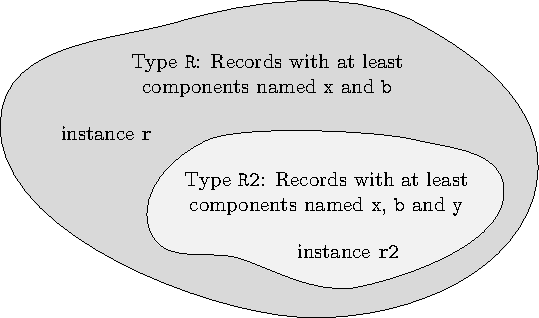
\includegraphics{subtype}
  \end{center}
  \caption{The type \lstinline!R! can be defined as the set of record values containing \lstinline!x! and \lstinline!b!.  The subtype \lstinline!R2! is the subset of values that all contain
  \lstinline!x!, \lstinline!b!, and \lstinline!y!.}
\end{figure}
\end{example}

\section{Interface or Type}\label{interface-or-type}

Based on a flattened class or component we can construct an interface
for that flattened class or component. The interface or type
(the terms \emph{interface} and \emph{type} are equivalent and can be used
interchangeably) is defined as the following information about the
flattened element itself:
\begin{itemize}
\item
  Whether it is replaceable or not.
\item
  Whether the class itself or the class of the component is transitively
  non-replaceable (\cref{transitively-non-replaceable}), and if not, the reference to the
  replaceable class it refers to.
\item
  Whether it is a component or a class.
\item
  Additional information about the element:

  \begin{itemize}
  \item
    The \lstinline!flow! or \lstinline!stream! prefix.
  \item
    Declared variability (\lstinline!constant!, \lstinline!parameter!, \lstinline!discrete!).
  \item
    The prefixes \lstinline!input! and \lstinline!output!.
  \item
    The prefixes \lstinline!inner! and/or \lstinline!outer!.
  \item
    Whether the declaration is \lstinline!final!, and in that case its semantics
    contents.
  \item
    Array sizes (if any).
  \item
    Condition of conditional components (if any).
  \item
    Which kind of specialized class.
  \item
    For an enumeration type or component of enumeration type the names
    of the enumeration literals in order.
  \item
    Whether it is a built-in type and the built-in type (\lstinline!RealType!,
    \lstinline!IntegerType!, \lstinline!StringType! or \lstinline!BooleanType!).
  \end{itemize}
\item
  Only for an \lstinline!operator record! class and classes derived from \lstinline!ExternalObject!: the full name of the operator record base-class
  (i.e.\  the one containing the operations), or the derived class.  See \cref{overloaded-operators} and \cref{external-objects}.

  The following item does not apply for an \lstinline!operator record! class or class derived from \lstinline!ExternalObject!, since the type is already
  uniquely defined by the full name.
\item
  For each named public element of the class or component (including
  both local and inherited named elements) a tuple comprised of:
  \begin{itemize}
  \item
    Name of the element.
  \item
    Interface or type of the element.
    \begin{nonnormative}
    This might have been modified by modifiers and is thus not necessarily identical to the interface of the original declaration.
    \end{nonnormative}
  \end{itemize}
\end{itemize}

The corresponding \emph{constraining} interface is constructed based on the \emph{constraining} type (\cref{constraining-type}) of the declaration (if replaceable -- otherwise same as actual
type) and with the \emph{constraining} interface for the named elements.

In a class all references to elements of that class should be limited to their constraining interface.

\begin{nonnormative}
The \emph{constraining interface} constsists of only the public elements, and if the declaration is replaceable the element is limited to the constraining interface.
\end{nonnormative}

\begin{nonnormative}
The public interface does not contain all of the information about the class or component.  When using a class as a base-class we also need protected elements, and
for internal type-checking we need e.g.\ import-elements.  However, the information is sufficient for checking compatibility and for using the class to flatten components.
\end{nonnormative}

\subsection{Transitively non-Replaceable}\label{transitively-non-replaceable}

\begin{nonnormative}
In several cases it is important that no new elements can be
added to the interface of a class, especially considering short class
definitions. Such classes are defined as transitively
non-replaceable.
\end{nonnormative}

A class reference is transitively non-replaceable iff (i.e.\ \emph{if and
only if}) all parts of the name satisfy the following:
\begin{itemize}
\item
  If the class definition is long it is transitively non-replaceable if
  not declared replaceable.
\item
  If the class definition is short (i.e.\ \lstinline!class A = P.B!) it is
  transitively non-replaceable if it is non-replaceable and equal to
  class reference (\lstinline!P.B!) that is transitively non-replaceable.
\end{itemize}

\begin{nonnormative}
According to \cref{restrictions-on-base-classes-and-constraining-types-to-be-transitively-non-replaceable}, for a hierarchical name all
parts of the name must be transitively non-replaceable, i.e.\ in \lstinline!extends A.B.C! this implies that \lstinline!A.B.C! must be transitively
non-replaceable, as well as \lstinline!A! and \lstinline!A.B!, with the exception of the \emph{class
extends redeclaration mechanism} see \cref{the-class-extends-redeclaration-mechanism}.
\end{nonnormative}

\subsection{Inheritance Interface or Class Type}\label{inheritance-interface-or-class-type}

For inheritance the interface also must include protected elements; this
is the only change compared to above.

Based on a flattened class we can construct an inheritance interface or
class type for that flattened class. The inheritance interface or class
type is defined as the following information about the flattened element
itself:
\begin{itemize}
\item
  Whether it is replaceable or not.
\item
  Whether the class itself or the class of the component is transitively
  non-replaceable (\cref{transitively-non-replaceable}), and if not the reference to
  replaceable class it refers to.
\item
  For each named element of the class (including both local and
  inherited named elements) a tuple comprised of:
  \begin{itemize}
  \item
    Name of the element.
  \item
    Whether the element is component or a class.
  \item
    For elements that are classes: Inheritance interface or class type of the element.
    \begin{nonnormative}
    This might have been modified by modifiers and is thus not necessarily identical to the interface of the original declaration.
    \end{nonnormative}
  \item
    For elements that are components: interface or type of the element.
    \begin{nonnormative}
    This might have been modified by modifiers and is thus not necessarily identical to the interface of the original declaration.
    \end{nonnormative}
  \end{itemize}
\item
  Additional information about the element:
  \begin{itemize}
  \item
    The \lstinline!flow! or \lstinline!stream! prefix.
  \item
    Declared variability (\lstinline!constant!, \lstinline!parameter!, \lstinline!discrete!).
  \item
    The prefixes \lstinline!input! and \lstinline!output!.
  \item
    The prefixes \lstinline!inner! and/or \lstinline!outer!.
  \item
    Whether the declaration is \lstinline!final!, and in that case its semantics
    contents.
  \item
    Array sizes (if any).
  \item
    Condition of conditional components (if any).
  \item
    Which kind of specialized class.
  \item
    For an enumeration type or component of enumeration type the names
    of the enumeration literals in order.
  \item
    Whether it is a built-in type and the built-in type (\lstinline!RealType!,
    \lstinline!IntegerType!, \lstinline!StringType! or \lstinline!BooleanType!).
  \item
    Visibility (\lstinline!public! or \lstinline!protected!).
  \end{itemize}
\end{itemize}

\section{Interface Compatibility or Subtyping}\label{interface-compatibility-or-subtyping}

An interface of a class or component \lstinline!A! is compatible with an interface
of a class or component \lstinline!B! (or the constraining interface of \lstinline!B!), or
equivalently that the type of \lstinline!A! is a subtype of the type of \lstinline!B!, iff:
\begin{itemize}
\item
  \lstinline!A! is a class if and only if \lstinline!B! is a class (and thus: \lstinline!A! is a component
  if and only if \lstinline!B! is a component).
\item
  If \lstinline!A! has an \lstinline!operator record! base-class then \lstinline!B! must also have one and
  it must be the same. If \lstinline!A! does not have an operator record base-class
  then \lstinline!B! shall not have one. See \cref{overloaded-operators}.
\item
  If \lstinline!A! is derived from \lstinline!ExternalObject!, then \lstinline!B! must also be derived from
  \lstinline!ExternalObject! and have the same full name. If \lstinline!A! is not derived from
  \lstinline!ExternalObject! then \lstinline!B! shall not be derived from \lstinline!ExternalObject!. See
  \cref{external-objects}.
\item
  If \lstinline!B! is not replaceable then \lstinline!A! shall not be replaceable.
\item
  If \lstinline!B! is transitively non-replaceable then \lstinline!A! must be transitively
  non-replaceable (\cref{transitively-non-replaceable}). For all elements of the inheritance
  interface of \lstinline!B! there must exist a compatible element with the same
  name and visibility in the inheritance interface of \lstinline!A!. The interface
  of \lstinline!A! shall not contain any other elements.
  \begin{nonnormative}
  We might even extend this to say that \lstinline!A! and \lstinline!B! should have the same contents, as in the additional restrictions below.
  \end{nonnormative}
\item
  If \lstinline!B! is replaceable then for all elements of the component interface
  of \lstinline!B! there must exist a plug-compatible element with the same name in
  the component interface of \lstinline!A!.
\item
  If \lstinline!B! is neither transitively non-replaceable nor replaceable then \lstinline!A!
  must be linked to the same class, and for all elements of the
  component interface of \lstinline!B! there must thus exist a plug-compatible
  element with the same name in the component interface of \lstinline!A!.
\item
  Additional restrictions on the additional information. These elements
  should either match or have a natural total order:

  \begin{itemize}
  \item
    If \lstinline!B! is a non-replaceable long class definition \lstinline!A! must also be a
    long class definition.
  \item
    The \lstinline!flow! or \lstinline!stream! prefix should be matched for compatibility.
  \item
    Variability is ordered \lstinline!constant! \textless{} \lstinline!parameter! \textless{}
    \lstinline!discrete! \textless{} continuous-time (\lstinline!Real! without prefix), and \lstinline!A! is
    only compatible with \lstinline!B! if the declared variability in \lstinline!A! is less than
    or equal the variability in \lstinline!B!.
    \begin{nonnormative}
    For a redeclaration of an element the variability prefix is as default inherited by the redeclaration (i.e.\ no need to repeat \lstinline!parameter!
    when redeclaring a parameter).
    \end{nonnormative}
  \item
    The input and output prefixes must be matched. This ensures that the
    rules regarding inputs/outputs for matching connectors and
    (non-connector inputs) are preserved, as well as the restriction on
    blocks.
    \begin{nonnormative}
    For a redeclaration of an element the input or output prefix is inherited from the original declaration.
    \end{nonnormative}
  \item
    The \lstinline!inner! and/or \lstinline!outer! prefixes should be matched.
    \begin{nonnormative}
    For a redeclaration of an element the \lstinline!inner! and/or \lstinline!outer! prefixes are inherited from the original declaration (since it is not
    possible to have \lstinline!inner! and/or \lstinline!outer! as part of a redeclare).
    \end{nonnormative}
  \item
    If \lstinline!B! is final \lstinline!A! must also be final and have the same semantic
    contents.
  \item
    The number of array dimensions in \lstinline!A! and \lstinline!B! must be matched.
  \item
    Conditional components are only compatible with conditional components.  The conditions must have equivalent contents (similar to array sizes, except there is no \lstinline!:! for conditional
    components).
    \begin{nonnormative}
    For a redeclaration of an element the conditional part is inherited from the original.
    \end{nonnormative}
  \item
    A \lstinline!function! class is only compatible with a \lstinline!function! class, a \lstinline!package! class only compatible with a \lstinline!package! class, a \lstinline!connector! class only with a \lstinline!connector! class, a \lstinline!model! or \lstinline!block! class only compatible with a \lstinline!model! or \lstinline!block! class, and a \lstinline!type! or \lstinline!record! class only compatible with a \lstinline!type! or \lstinline!record! class.
  \item
    If \lstinline!B! is an enumeration type \lstinline!A! must also be an enumeration type and
    vice versa. If \lstinline!B! is an enumeration type not defined as \lstinline!(:)! then \lstinline!A!
    must have the same enumeration literals in the same order; if \lstinline!B! is
    an enumeration type defined as \lstinline!(:)! then there is no restriction on
    the enumeration type \lstinline!A!.
  \item
    If \lstinline!B! is a built-in type then \lstinline!A! must also be of the same built-in
    type and vice versa.
  \end{itemize}
\end{itemize}

\begin{nonnormative}
Intuitively, that the type \lstinline!A! is a subtype of the type of \lstinline!B! means that all important elements of \lstinline!B! are be present in \lstinline!A!.
\end{nonnormative}

Plug-compatibility is a further restriction of compatibility (subtyping)
defined in \cref{plug-compatibility-or-restricted-subtyping}, and further restricted for functions, see
\cref{function-compatibility-or-function-subtyping-for-functions}. For a replaceable declaration or modifier the default class
must be compatible with the constraining class.

For a modifier the following must apply:
\begin{itemize}
\item
  The modified element should exist in the element being modified.
\item
  The modifier should be compatible with the element being modified, and
  in most cases also plug-compatible, \cref{plug-compatibility-or-restricted-subtyping}.
\end{itemize}

\begin{nonnormative}
If the original constraining flat class is legal (no references to unknown elements and no illegal use of class/component), and modifiers legal as above, then the resulting flat class will be legal
(no references to unknown elements and no illegal use of class/component and compatible with original constraining class) and references refer to similar entities.
\end{nonnormative}

\section{Plug-Compatibility or Restricted Subtyping}\label{plug-compatibility-or-restricted-subtyping}

\begin{nonnormative}
If a sub-component is redeclared, see \cref{redeclaration}, it is
impossible to connect to any new connector. A connector with input
prefix must be connected to, and since one cannot connect across
hierarchies, one should not be allowed to introduce such a connector at
a level where a connection is not possible. Therefore all public
components present in the interface A that are not present in B must be
connected by default.
\end{nonnormative}

\begin{definition}[Plug-compatibility (= restricted subtyping)]
An interface \lstinline!A! is plug-compatible with (a restricted subtype of) an
interface \lstinline!B! (or the constraining interface of \lstinline!B!) iff:
\begin{itemize}
\item
  \lstinline!A! is compatible with (subtype of) \lstinline!B!.
\item
  All public components present in \lstinline!A! but not in \lstinline!B! must be
  default-connectable (as defined below).
\end{itemize}
\end{definition}

\begin{definition}[Default connectable]
A component of an interface is default-connectable iff:
\begin{itemize}
\item
  All of its components are default connectable.
\item
  A connector component must not be an \lstinline!input!.
  \begin{nonnormative}
  Otherwise a connection to the input will be missing.
  \end{nonnormative}
\item
  A connector component must not be of an expandable connector class.
  \begin{nonnormative}
  The expandable connector does potentially have inputs.
  \end{nonnormative}
\item
  A parameter, constant, or non-connector input must either have a
  binding equation or all of its sub-components must have binding
  equations.
\end{itemize}
\end{definition}

Based on the above definitions, there are the following restrictions:
\begin{itemize}
\item
  A redeclaration of an inherited top-level component must be
  \emph{compatible} \emph{with} (subtype of) the constraining interface
  of the element being redeclared.
\item
  In all other cases redeclarations must be \emph{plug-compatible} with
  the constraining interface of the element being redeclared.
\end{itemize}

\begin{nonnormative}
The reason for the difference is that for an inherited
top-level component it is possible to connect to the additional
connectors, either in this class or in a derived class.

Example:
\begin{lstlisting}[language=modelica]
partial model TwoFlanges
  Modelica.Mechanics.Rotational.Interfaces.Flange_a flange_a;
  Modelica.Mechanics.Rotational.Interfaces.Flange_b flange_b;
end TwoFlanges;

partial model FrictionElement
  extends TwoFlanges;
  ...
end FrictionElement;

model Clutch "compatible - but not plug-compatible with FrictionElement"
  Modelica.Blocks.Interfaces.RealInput pressure;
  extends FrictionElement;
  ...
end Clutch;

model DriveLineBase
  extends TwoFlanges;
  Inertia J1;
  replaceable FrictionElement friction;
equation
  connect(flange_a, J1.flange_a);
  connect(J1.flange_b, friction.flange_a);
  connect(friction.flange_b, flange_b);
end DriveLineBase;

model DriveLine
  extends DriveLineBase(redeclare Clutch friction);
  Constant const;
equation
  connect(const.y, frition.pressure);
  // Legal connection to new input connector.
end DriveLine;

model UseDriveLine "illegal model"
  DriveLineBase base(redeclare Clutch friction);
  // Cannot connect to friction.pressure
end UseDriveLine;
\end{lstlisting}

If a subcomponent is redeclared, it is impossible to connect to
any new connector. Thus any new connectors must work without being
connected, i.e., the default connection of flow-variables. That fails
for inputs (and expandable connectors may contain inputs). For
parameters and non-connector inputs it would be possible to provide
bindings in a derived class, but that would require hierarchical
modifiers and it would be bad modeling practice that a hierarchical
modifier must be used in order to make a model valid. A replaceable
class might be used as the class for a sub-component, therefore
plug-compatibility is required not only for replaceable sub-components,
but also for replaceable classes.
\end{nonnormative}

\section{Function-Compatibility or Function-Subtyping for Functions}\label{function-compatibility-or-function-subtyping-for-functions}

\begin{nonnormative}
Functions may be called with either named or positional
arguments, and thus both the name and order is significant. If a
function is redeclared, see \cref{redeclaration}, any new arguments must
have defaults (and be at the end) in order to preserve the meaning of
existing calls.
\end{nonnormative}

\begin{definition}[Function-compatibility or function-subtyping for functions]
A function class \lstinline!A! is \emph{function-compatible with or a function
subtype of} function class \lstinline!B! iff (the terms \emph{function-compatible}
and \emph{function subtype} of are synonyms and used interchangeably):
\begin{itemize}
\item
  \lstinline!A! is compatible to (subtype of) \lstinline!B!.
\item
  All public input components of \lstinline!B! have correspondingly named public
  input components of \lstinline!A! in the same order and preceding any additional
  public input components of \lstinline!A!.
\item
  All public output components of \lstinline!B! have correspondingly named public
  output components of \lstinline!A! in the same order and preceding any additional
  public output components of \lstinline!A!.
\item
  A public input component of \lstinline!A! must have a binding assignment if the
  corresponding named element has a binding assignment in \lstinline!B!.
\item
  A public input component of \lstinline!A! not present in \lstinline!B! must have a binding
  assignment.
\end{itemize}
\end{definition}

Based on the above definition the following restriction holds:
\begin{itemize}
\item
  The interface of a redeclared function must be
  \emph{function-compatible with or a function subtype of} the
  constraining interface of the function being redeclared.
\end{itemize}

\begin{example}
Demonstrating a redeclaration using a function-compatible function
\begin{lstlisting}[language=modelica]
function GravityInterface
  input Modelica.Units.SI.Position position[3];
  output Modelica.Units.SI.Acceleration acceleration[3];
end GravityInterface;

function PointMassGravity
  extends GravityInterface;
  input Modelica.Units.SI.Mass m;
algorithm
  acceleration := -Modelica.Constants.G*m*position/(position*position)^1.5;
end PointMassGravity;

model Body
  model UseDriveLine "illegal model"
    DriveLineBase base(redeclare Clutch friction);
    // Cannot connect to friction.pressure
  end UseDriveLine;
  Modelica.Mechanics.MultiBody.Interface.Frame_a frame_a;
  replaceable function gravity = GravityInterface;
equation
  frame_a.f = gravity(frame_a.r0);
  // or gravity(position=frame_a.r0);
  frame_a.t = zeros(3);
end Body;

model PlanetSimulation
  function sunGravity = PointMassGravity (m=2e30);
  Body planet1(redeclare function gravity = sunGravity);
  Body planet2(redeclare function gravity = PointMassGravity (m=2e30));
  ...
end PlanetSimulation;
\end{lstlisting}

Note: \lstinline!PointMassGravity! is not function-compatible with
\lstinline!GravityInterface! (no default for \lstinline!m!), but \lstinline!sunGravity!
inside \lstinline!PlanetSimulation! is function-compatible with
\lstinline!GravityInterface!.
\end{example}

\section{Type Compatible Expressions}\label{type-compatible-expressions}

Certain expressions consist of an operator applied to two or more type
compatible sub-expressions (\lstinline!A! and \lstinline!B!), including binary operators, e.g.
\lstinline!A + B!, if-expressions, e.g.\ \lstinline!if x then A else B!, and array expressions,
e.g.\ \lstinline!{A, B}!. The resulting type of the expression in case of two type
compatible subexpressions \lstinline!A! and \lstinline!B! is defined as follows:
\begin{itemize}
\item
  If \lstinline!A! is a record-expression \lstinline!B! must also be a record-expression with
  the same named elements. The type compatible expression is a record
  comprised of named elements that are compatible with the corresponding
  named elements of both \lstinline!A! and \lstinline!B!.
\item
  If \lstinline!A! is an array expression then \lstinline!B! must also be an array expression,
  and \lstinline!ndims(A)! = \lstinline!ndims(B)!. The type compatible expression is an array
  expression with elements compatible with the elements of both \lstinline!A! and \lstinline!B!.
  If both \lstinline!size(A)! and \lstinline!size(B)! are known
	and \lstinline!size(A)! = \lstinline!size(B)! then this
  defines the size of the type compatible expression, otherwise the size
  of the expression is not known until the expression is about to be
  evaluated. In case of an if-expression the size of the type compatible
  expression is defined based on the branch selected, and for other
  cases \lstinline!size(A)! = \lstinline!size(B)! must hold at this point.
\item
  If \lstinline!A! is a scalar expression of a simple type \lstinline!B! must also be a scalar
  expression of a simple type.
\item
  If \lstinline!A! is a \lstinline!Real! expression then \lstinline!B! must be a \lstinline!Real! or \lstinline!Integer! expression
  and the type compatible expression is \lstinline!Real!, compare \cref{standard-type-coercion}.
\item
  If \lstinline!A! is an \lstinline!Integer! expression then \lstinline!B! must be a \lstinline!Real! or \lstinline!Integer!
  expression. For exponentiation and division the type compatible
  expression is \lstinline!Real! (even if both \lstinline!A! and \lstinline!B! are \lstinline!Integer!) see \cref{exponentiation-of-scalars-of-numeric-elements}
  and \cref{division-of-scalars-or-numeric-arrays-by-numeric-scalars}, in
  other cases the type compatible expression is \lstinline!Real! or \lstinline!Integer! (same as
  \lstinline!B!), compare \cref{standard-type-coercion}.
\item
  If \lstinline!A! is a \lstinline!Boolean! expression then \lstinline!B! must be a \lstinline!Boolean! expression and
  the type compatible expression is \lstinline!Boolean!.
\item
  If \lstinline!A! is a \lstinline!String! expression then \lstinline!B! must be a \lstinline!String! expression and the
  type compatible expression is \lstinline!String!.
\item
  If \lstinline!A! is an enumeration expression then \lstinline!B! must be an enumeration
  expression and the type compatible expression is enumeration
  expression, and all enumeration expressions must be defined in terms
  of an enumeration type with the same enumeration literals in the same
  order.
\item
  If \lstinline!A! has an \lstinline!operator record! base-class then \lstinline!B! must also have an
  \lstinline!operator record! base-class, and it must be the same, and otherwise
  neither \lstinline!A! nor \lstinline!B! may have an \lstinline!operator record! base-class. This is also
  the \lstinline!operator record! base-class for the expression e.g.\ for
  \lstinline!if (cond) then A else B!.
\item
  If \lstinline!A! is derived from \lstinline!ExternalObject! then \lstinline!B! must also be derived from
  \lstinline!ExternalObject! and they must have the same full name; and otherwise
  neither \lstinline!A! nor \lstinline!B! may be derived from \lstinline!ExternalObject!. The common full
  name also defines the type of the expression, e.g.\ for \lstinline!if (cond) then A else B!.
\end{itemize}


% Inheritance, Modification, and Redeclaration
\chapter{Inheritance, Modification, and Redeclaration}\label{inheritance-modification-and-redeclaration}

One of the major benefits of object-orientation is the ability to \emph{extend} the behavior and properties of an existing class.
The original class, known as the \willintroduce{base class}, is extended to create a more specialized version of that class, known as the \willintroduce{derived class}.
In this process, the data and behavior of the original class in the form of variable declarations, equations, and certain other contents are reused, or \emph{inherited}, by the derived class.
In fact, the inherited contents is copied from the superclass into the derived class, but before copying certain operations, such as type expansion, checking, and modification, are performed on the inherited contents when appropriate.
This chapter describes the inheritance concept in Modelica, together with the related concepts modification and redeclaration.

\section{Inheritance -- Extends Clause}\label{inheritance-extends-clause}

The class \lstinline!A! is called a \firstuse{base class}\index{base class} of \lstinline!B!, if \lstinline!B! extends \lstinline!A!.
The converse relation is then expressed as \lstinline!B! being a \firstuse{derived class}\index{derived class} of \lstinline!A!, or as \lstinline!B! being \firstuse{derived from} \lstinline!A!.
This relation is specified by an extends-clause in \lstinline!B! or in one of \lstinline!B!'s base classes.
A class inherits all elements from its base classes, and may modify all non-final elements inherited from base classes, as explained below.

The \firstuse{extends-clause}\index{extends-clause} is used to specify inheritance from a base class into an (enclosing) class containing the extends-clause.
It is an unnamed element of a class definition that uses a name and an optional modification to specify a base class of the class defined using the class definition.
The syntax of the extends-clause is as follows:
\begin{lstlisting}[language=grammar]
extends-clause :
   extends name [ class-modification ] [annotation]
\end{lstlisting}%
\indexinline{extends}
The name of the base class is looked up in the partially flattened
enclosing class (\cref{enclosing-classes}) of the extends-clause. The found base
class is flattened with a new environment and the partially flattened
enclosing class of the extends-clause. The new environment is the result
of merging
\begin{itemize}
\item
  arguments of all enclosing class environments that match names in the
  flattened base class
\item
  the optional \lstinline!class-modification! of the extends-clause
\end{itemize}
in that order.

\begin{example}
\begin{lstlisting}[language=modelica]
class A
  parameter Real a, b;
end A;

class B
  extends A(b = 2);
end B;

class C
  extends B(a = 1);
end C;
\end{lstlisting}
\end{example}

The elements of the flattened base class become elements of the flattened enclosing class, and are added at the place of the extends-clause: specifically components and classes, the equation sections, algorithm sections, optional external-clause, and the contents of the annotation at the end of the class, but excluding import-clauses.

\begin{nonnormative}
From the example above we get the following flattened class:
\begin{lstlisting}[language=modelica]
class Cinstance
  parameter Real a = 1;
  parameter Real b = 2;
end Cinstance;
\end{lstlisting}

The ordering of the merging rules ensures that, given classes \lstinline!A! and \lstinline!B! defined above,
\begin{lstlisting}[language=modelica]
class C2
  B bcomp(b = 3);
end C2;
\end{lstlisting}
yields an instance with \lstinline!bcomp.b = 3!, which overrides \lstinline!b = 2!.
\end{nonnormative}

The declaration elements of the flattened base class shall either:
\begin{itemize}
\item
  Not already exist in the partially flattened enclosing class
  (i.e., have different names).
\item
  The new element is a long form of redeclare or uses the \lstinline!class extends A! syntax, see \cref{redeclaration}.
\item
  Be exactly identical to any element of the flattened enclosing class
  with the same name and the same level of protection (public or
  protected) and same contents. In this case, the first element in order
  (can be either inherited or local) is kept. It is recommended to give
  a warning for this case; unless it can be guaranteed that the
  identical contents will behave in the same way.
\end{itemize}

Otherwise the model is incorrect.

\begin{nonnormative}
Clarifiying order:
\begin{lstlisting}[language=modelica]
function A
  input Real a;
  input Real b;
end A;

function B
  extends A;
  input Real a;
end B;
// The inputs of B are "a, b" in that order; and the "input Real a;" is ignored.
\end{lstlisting}
\end{nonnormative}

Equations of the flattened base class that are syntactically equivalent
to equations in the flattened enclosing class are discarded. This
feature is deprecated, and it is recommended to give a warning when
discarding them and for the future give a warning about all forms of
equivalent equations due to inheritance.

\begin{nonnormative}
Equations that are mathematically equivalent but not syntactically equivalent are not discarded, hence yield an overdetermined system of equations.
\end{nonnormative}

\subsection{Multiple Inheritance}\label{multiple-inheritance}

Multiple inheritance is possible since multiple extends-clauses can be
present in a class.

\subsection{Inheritance of Protected and Public Elements}\label{inheritance-of-protected-and-public-elements}

If an extends-clause is used under the \lstinline!protected! heading, all elements
of the base class become protected elements of the current class. If an
extends-clause is a public element, all elements of the base class are
inherited with their own protection. The eventual headings \lstinline!protected! and
\lstinline!public! from the base class do not affect the consequent elements of the
current class (i.e., headings \lstinline!protected! and \lstinline!public! are not inherited).

\subsection{Restrictions on the Kind of Base Class}\label{restrictions-on-the-kind-of-base-class}

Since specialized classes of different kinds have different properties,
see \cref{specialized-classes}, only specialized classes that are \emph{in some sense
compatible} to each other can be derived from each other via
inheritance. The following table shows which kind of specialized class
can be used in an extends clause of another kind of specialized class
(the grey cells mark the few exceptional cases, where a specialized
class can be derived from a specialized class of another kind):
% The PDF contains an excessive amount of vertical space here, but it seems like a bad idea to try to make it go away
% by adding LaTeX spacing commands that will cause problems later when things move around.
\begin{center}
% LaTeXML does not handle resizebox, so don't use it for HTML.
\ifpdf\resizebox{\textwidth}{!}{\else\fi%
\begin{tabular}{|c||c|c|c|c|c|c|c|c|c|c|c|c|}
    \hline
                      & \multicolumn{12}{c|}{\tablehead{Base Class}}                                                                                                                                                                                                                                                                                                                          \\
    \hline
     \tablehead{Derived} & \multirow{2}{*}{\lstinline!package!} & \multirow{2}{*}{\lstinline!operator!} & \multirow{2}{*}{\lstinline!function!}                  & \lstinline!operator!             & \multirow{2}{*}{\lstinline!type!}    & \multirow{2}{*}{\lstinline!record!}  & \lstinline!operator!                 & \lstinline!expandable!               & \multirow{2}{*}{\lstinline!connector!} & \multirow{2}{*}{\lstinline!block!}   & \multirow{2}{*}{\lstinline!model!} & \multirow{2}{*}{\lstinline!class!}                     \\
     \tablehead{Class}   &                          &                           &                                            & \lstinline!function!             &                          &                          & \lstinline!record!                   & \lstinline!connector!                &                            &                          &                        &                                            \\
    \hline
    \hline
    \lstinline!package!           & yes                      &                           &                                            &                      &                          &                          &                          &                          &                            &                          &                        & \cellcolor{lightgray}yes                   \\
    \hline
    \lstinline!operator!          &                          & yes                       &                                            &                      &                          &                          &                          &                          &                            &                          &                        & \cellcolor{lightgray}yes                   \\
    \hline
    \lstinline!function!          &                          &                           & yes                                        &                      &                          &                          &                          &                          &                            &                          &                        & \cellcolor{lightgray}yes                   \\
    \hline
    \lstinline!operator!          &                          &                           & \cellcolor{lightgray}                      & \multirow{2}{*}{yes} &                          &                          &                          &                          &                            &                          &                        & \cellcolor{lightgray}                      \\
    \lstinline!function!          &                          &                           & \multirow{-2}{*}{\cellcolor{lightgray}yes} &                      &                          &                          &                          &                          &                            &                          &                        & \multirow{-2}{*}{\cellcolor{lightgray}yes}  \\
    \hline
    \lstinline!type!              &                          &                           &                                            &                      & yes                      &                          &                          &                          &                            &                          &                        & \cellcolor{lightgray}yes                   \\
    \hline
    \lstinline!record!            &                          &                           &                                            &                      &                          & yes                      &                          &                          &                            &                          &                        & \cellcolor{lightgray}yes                   \\
    \hline
    \lstinline!operator!          &                          &                           &                                            &                      &                          &                          & \multirow{2}{*}{yes}     &                          &                            &                          &                        & \cellcolor{lightgray}                      \\
    \lstinline!record!            &                          &                           &                                            &                      &                          &                          &                          &                          &                            &                          &                        & \multirow{-2}{*}{\cellcolor{lightgray}yes} \\
    \hline
    \lstinline!expandable!        &                          &                           &                                            &                      &                          &                          &                          & \multirow{2}{*}{yes}     &                            &                          &                        & \cellcolor{lightgray}                      \\
    \lstinline!connector!         &                          &                           &                                            &                      &                          &                          &                          &                          &                            &                          &                        & \multirow{-2}{*}{\cellcolor{lightgray}yes} \\
    \hline
    \lstinline!connector!         &                          &                           &                                            &                      & \cellcolor{lightgray}yes & \cellcolor{lightgray}yes & \cellcolor{lightgray}yes &                          & yes                        &                          &                        & \cellcolor{lightgray}yes                   \\
    \hline
    \lstinline!block!             &                          &                           &                                            &                      &                          & \cellcolor{lightgray}yes &                          &                          &                            & yes                      &                        & \cellcolor{lightgray}yes                   \\
    \hline
    \lstinline!model!             &                          &                           &                                            &                      &                          & \cellcolor{lightgray}yes &                          &                          &                            & \cellcolor{lightgray}yes & yes                    & \cellcolor{lightgray}yes                   \\
    \hline
    \lstinline!class!             &                          &                           &                                            &                      &                          &                          &                          &                          &                            &                          &                        & yes                                        \\
    \hline
\end{tabular}
% Close resizebox.
\ifpdf}\else\fi%
\end{center}

If a derived class is inherited from another type of specialized class,
then the result is a specialized class of the derived class type.

\begin{nonnormative}
For example, if a \lstinline!block! inherits from a \lstinline!record!, then the result is a \lstinline!block!.
\end{nonnormative}

All specialized classes can be derived from \lstinline!class!\indexinline{class}, provided that the resulting class fulfills the restriction of the specialized class.
A \lstinline!class! may only contain class-definitions, annotations, and extends-clauses (having any other contents is deprecated).

\begin{nonnormative}
It is recommended to use the most specific specialized class.
\end{nonnormative}

The specialized classes \lstinline!package!, \lstinline!operator!, \lstinline!function!,
\lstinline!type,! \lstinline!record!,
\lstinline!operator record!, and \lstinline!expandable connector! can only be derived from their
own kind and from \lstinline!class!.

\begin{nonnormative}
E.g.\ a package can only be base class for packages.  All other kinds of classes can use the import-clause to use the contents of a package.
\end{nonnormative}

\begin{example}
\begin{lstlisting}[language=modelica]
record RecordA
  ...
end RecordA;

package PackageA
  ...
end PackageA;

package PackageB
  extends PackageA; // fine
end PackageB;

model ModelA
  extends RecordA; // fine
end ModelA;

model ModelB
  extends PackageA; // error, inheritance not allowed
end ModelB;
\end{lstlisting}
\end{example}

\subsection{Restrictions on Base Classes and Constraining Types to be Transitively Non-Replaceable}\label{restrictions-on-base-classes-and-constraining-types-to-be-transitively-non-replaceable}

The class name used after \lstinline!extends! for base-classes and for constraining classes must use a class reference considered transitively non-replaceable, see definition in \cref{transitively-non-replaceable}.  For a replaceable component declaration without constraining clause the class must use a class reference considered transitively non-replaceable.

\begin{nonnormative}
The requirement to use a transitively non-replaceable name excludes the long form of redeclare, i.e.\ \lstinline!redeclare model extends M...! where
\lstinline!M! must be an inherited replaceable class.
\end{nonnormative}

\begin{nonnormative}
The rule for a replaceable component declaration without constraining clause implies that constraining classes are always transitively non-replaceable -- both
if explicitly given or implicitly by the declaration.
\end{nonnormative}

\section{Modifications}\label{modifications}

A \firstuse{modification}\index{modification} is part of an element.
It modifies the instance generated by that element.
A modification contains \willintroduce{element modifications} (e.g., \lstinline!vcc(unit = "V") = 1000!) and \willintroduce{element-redeclarations} (e.g., \lstinline!redeclare type Voltage = Real(unit="V")!).

There are three kinds of constructs in the Modelica language in which modifications can occur:
\begin{itemize}
\item
  Variable declarations.
\item
  Short class declarations.
\item
  Extends-clauses.
\end{itemize}

A modifier modifies one or more declarations from a class by changing
some aspect(s) of the declarations. The most common kind of modifier
just changes the \emph{default value} or the \emph{start value} in a
binding equation; the value and/or start-value should be compatible with
the variable according to \cref{type-compatible-expressions}.

An \firstuse{element modification}\index{element modification} overrides the declaration equation in the class used by the instance generated by the modified element.

\begin{example}
Modifying the default \lstinline!start! value of the \lstinline!altitude! variable:
\begin{lstlisting}[language=modelica]
Real altitude(start = 59404);
\end{lstlisting}
\end{example}

A modification (e.g., \lstinline!C1 c1(x = 5)!) is called a \firstuse{modification equation}\index{modification equation}, if the modified variable (here: \lstinline!c1.x!) is a non-parameter variable.

\begin{nonnormative}
The modification equation is created, if the modified component (here: \lstinline!c1!) is also created (see \cref{class-declarations}). In most cases
a modification equation for a non-parameter variable requires that the variable was declared with a declaration equation, see \cref{balanced-models};
in those cases the declaration equation is replaced by the modification equation.
\end{nonnormative}

A more dramatic change is to modify the \emph{type} and/or the \emph{prefixes} and possibly the \emph{dimension sizes} of a declared element.
This kind of modification is called an \firstuse{element-redeclaration}\index{element-redeclaration}\index{redeclaration!element} (\cref{redeclaration}) and requires the special keyword \lstinline!redeclare! to be used in the modifier in order to reduce the risk for accidental modeling errors.
In most cases a declaration that can be redeclared must include the prefix \lstinline!replaceable!\indexinline{replaceable} (\cref{redeclaration}).
The modifier value (and class for redeclarations) is found in the context in which the modifier occurs, see also \cref{simple-name-lookup}.

\begin{example}
Scope for modifiers:
\begin{lstlisting}[language=modelica]
model B
  parameter Real x;
  package Medium = Modelica.Media.PartialMedium;
end B;

model C
  parameter Real x = 2;
  package Medium = Modelica.Media.PartialMedium;
  B b(x = x, redeclare package Medium = Medium);
  // The 'x' and 'Medium' being modified are declared in the model B.
  // The modifiers '= x' and '= Medium' are found in the model C.
end C;

model D
  parameter Real x = 3;
  package Medium = Modelica.Media.PartialMedium;
  C c(b(x = x, redeclare package Medium = Medium));
  // The 'x' and 'Medium' being modified are declared in the model B.
  // The modifiers '= x' and '= Medium' are found in the model D.
end D;
\end{lstlisting}
\end{example}

When present, the description-string of a modifier overrides the existing description.

\subsection{Syntax of Modifications and Redeclarations}\label{syntax-of-modifications-and-redeclarations}

The syntax is defined in the grammar, \cref{modification}.

\subsection{Modification Environment}\label{modification-environment}

The \firstuse{modification environment}\index{modification environment} of a class contains arguments which modify elements of the class (e.g., parameter changes) when the class is flattened.
The modification environment is built by merging class modifications, where outer modifications override inner modifications.

\begin{nonnormative}
This should not be confused with \lstinline!inner outer! prefixes described in \cref{instance-hierarchy-name-lookup-of-inner-declarations}.
\end{nonnormative}

\subsection{Merging of Modifications}\label{merging-of-modifications}

Merging of modifiers means that outer modifiers override inner modifiers.  The merging is hierarchical, and a value for an entire non-simple component overrides value modifiers for all components, and it is an error if this overrides a \lstinline!final! prefix for a component, or if value for a simple component would override part of the value of a non-simple component. When merging modifiers each modification keeps its own \lstinline!each! prefix.

\begin{example}
The following larger example demonstrates several aspects:
\begin{lstlisting}[language=modelica]
class C1
  class C11
    parameter Real x;
  end C11;
end C1;

class C2
  class C21
    $\ldots$
  end C21;
end C2;

class C3
  extends C1;
  C11 t(x = 3); // ok, C11 has been inherited from C1
  C21 u; // ok, even though C21 is inherited below
  extends C2;
end C3;
\end{lstlisting}
The following example demonstrates overriding part of non-simple component:
\begin{lstlisting}[language=modelica]
record A
  parameter Real x;
  parameter Real y;
end A;

model B
  parameter A a = A(2, 3);
end B;

model C
  B b1(a(x = 4)); // Error since attempting to override value for a.x when a has a value.
end C;
\end{lstlisting}

The modification environment of the declaration of \lstinline!t! is
(\lstinline!x = 3!). The modification environment is built by merging class modifications, as shown by:
\begin{lstlisting}[language=modelica]
class C1
  parameter Real a;
end C1;

class C2
  parameter Real b;
  parameter Real c;
end C2;

class C3
  parameter Real x1; // No default value
  parameter Real x2 = 2; // Default value 2
  parameter C1 x3; // No default value for x3.a
  parameter C2 x4(b = 4); // x4.b has default value 4
  parameter C1 x5(a = 5); // x5.a has default value 5
  extends C1; // No default value for inherited element a
  extends C2(b = 6, c = 77); // Inherited b has default value 6
end C3;

class C4
  extends C3(x2 = 22, x3(a = 33), x4(c = 44), x5 = x3, a = 55, b = 66);
end C4;
\end{lstlisting}

Outer modifications override inner modifications, e.g., \lstinline!b = 66!
overrides the nested class modification of extends \lstinline!C2(b = 6)!.
This is known as merging of modifications: merge\lstinline!((b = 66), (b = 6))!
becomes \lstinline!(b = 66)!.

A flattening of class \lstinline!C4! will give an object with the following variables:
\begin{center}
\begin{tabular}{l|l}
\hline
\tablehead{Variable} & \tablehead{Default value}\\
\hline
\hline
\lstinline!x1! & \textit{none}\\ % Look of \emph won't be as expected inside example.
\lstinline!x2! & 22\\
\lstinline!x3.a! & 33\\
\lstinline!x4.b! & 4\\
\lstinline!x4.c! & 44\\
\lstinline!x5.a! & \lstinline!x3.a!\\
\lstinline!a! & 55\\
\lstinline!b! & 66\\
\lstinline!c! & 77\\
\hline
\end{tabular}
\end{center}
\end{example}

\subsection{Single Modification}\label{single-modification}

Two arguments of a modification shall not modify the same element, attribute, or description-string.  When using qualified names the different qualified names starting with the same identifier are merged into one modifier.  If a modifier with a qualified name has the \lstinline!each! or \lstinline!final! prefix, that prefix is only seen as applied to the final part of the name.

\begin{example}
\begin{lstlisting}[language=modelica]
class C1
  Real x[3];
end C1;
class C2 = C1(x = ones(3), x = ones(3)); // Error: x designated twice
class C3
  class C4
    Real x;
  end C4;
  C4 a(final x.unit = "V", x.displayUnit = "mV", x = 5.0);
  // Ok, different attributes designated (unit, displayUnit and value)
  // identical to:
  C4 b(x(final unit = "V", displayUnit = "mV") = 5.0));
end C3;
\end{lstlisting}

The following examples are incorrect:
\begin{lstlisting}[language=modelica]
m1(r = 1.5, r = 1.6) // Multiple modifier for r (its value)
m1(r = 1.5, r = 1.5) // Multiple modifier for r (its value) - even if identical
m1(r.start = 2, r(start = 3)) // Multiple modifier for r.start
m1(x.r = 1.5 "x", x.r(start = 2.0) "y")) // Multiple description-string for x.r
m1(r = R(), r(y = 2)) // Multiple modifier for r.y - both direct value and
                      // part of record
\end{lstlisting}
The following examples are correct:
\begin{lstlisting}[language=modelica]
m1(r = 1.5, r(start = 2.0))
m1(r = 1.6, r "x")
m1(r = R(), r(y(min = 2)))
\end{lstlisting}
\end{example}

\subsection{Modifiers for Array Elements}\label{modifiers-for-array-elements}

The following rules apply to modifiers:
\begin{itemize}
\item
  The \lstinline!each!\indexinline{each} keyword on a modifier requires that it is applied in an array declaration/modification, and the modifier is applied individually to each element of the enclosing array (with regard to the position of \lstinline!each!).
  In case of nested modifiers this implies it is applied individually to each element of each element of the enclosing array; see example.
  If the modified element is a vector and the modifier does not contain the \lstinline!each!-prefix, the modification is split such that the first element in the vector is applied to the first element of the vector of elements, the second to the second element, until the last element of the vector-expression is applied to the last element of the array; it is an error if these sizes do not match.
  Matrices and general arrays of elements are treated by viewing those as vectors of vectors etc.
\item
  If a nested modifier is split, the split is propagated to all elements
  of the nested modifier, and if they are modified by the \lstinline!each!-keyword
  the split is inhibited for those elements. If the nested modifier that
  is split in this way contains re-declarations that are split it is
  illegal.
\end{itemize}

\begin{example}
\begin{lstlisting}[language=modelica]
model C
  parameter Real a [3];
  parameter Real d;
end C;

model B
  C c[5](each a = {1, 2, 3}, d = {1, 2, 3, 4, 5});
  parameter Real b = 0;
end B;
\end{lstlisting}
This implies \lstinline!c[i].a[j] = j! and \lstinline!c[i].d = i!.

\begin{lstlisting}[language=modelica]
model D
  B b(each c.a = {3, 4, 5}, c.d = {2, 3, 4, 5, 6});
  // Equivalent to:
  B b2(c(each a = {3, 4, 5}, d = {2, 3, 4, 5, 6}));
end D;
\end{lstlisting}
This implies \lstinline!b.c[i].a[j] = 2+j! and \lstinline!b.c[i].d = 1+i!.
\begin{lstlisting}[language=modelica]
model E
  B b[2](each c(each a = {1, 2, 3}, d = {1, 2, 3, 4, 5}), p = {1, 2});
  // Without the first each one would have to use:
  B b2[2](c(each a = {1, 2, 3}, d = fill({1, 2, 3, 4, 5}, 2)), p = {1, 2});
end E;
\end{lstlisting}
This implies \lstinline!b[k].c[i].a[j] = j!, \lstinline!b[k].c[i].d = i!, and \lstinline!b[k].p = k!.  For \lstinline!c.a! the additional (outer) \lstinline!each! has no effect, but it is necessary for \lstinline!c.d!.

Specifying array dimensions after the type works the same as specifying them after the variable name.
\begin{lstlisting}[language=modelica]
model F
  Real fail1[2](each start = {1, 2}); // Illegal
  Real work1[2](each start = 1);      // Legal
  Real[2] fail2(each start = {1, 2}); // Illegal
  Real[2] work2(each start = 2);      // Legal
end F;
\end{lstlisting}
\end{example}

\subsection{Final Element Modification Prevention}\label{final-element-modification-prevention}

An element defined as final by the \lstinline!final!\indexinline{final} prefix in an element modification or declaration cannot be modified by a modification or by a redeclaration.  All elements of a final element are also final.

\begin{nonnormative}
Setting the value of a parameter in an experiment environment is conceptually treated as a modification.  This implies that a final modification equation
of a parameter cannot be changed in a simulation environment.
\end{nonnormative}

\begin{example}
Final component modification.
\begin{lstlisting}[language=modelica]
type Angle =
  Real(final quantity = "Angle", final unit = "rad", displayUnit = "deg");

model TransferFunction
  parameter Real b[:] = {1} "numerator coefficient vector";
  parameter Real a[:] = {1, 1} "denominator coefficient vector";
  ...
end TransferFunction;

model PI "PI controller"
  parameter Real k = 1 "gain";
  parameter Real T = 1 "time constant";
  TransferFunction tf(final b = k * {T, 1}, final a = {T, 0});
end PI;

model Test
  PI c1(k = 2, T = 3); // fine, will indirectly change tf.b to 2 * {3, 1}
  PI c2(tf(b = {1}));  // error, b is declared as final
end Test;
\end{lstlisting}
\end{example}

\begin{example}
Final class declaration.
\begin{lstlisting}[language=modelica]
model Test2
  final model MyTF = TransferFunction(b = {1, 2});
  /* Equivalently:
  final model MyTF = TransferFunction(final a, final b = {1, 2});
  */
  MyTF tf1;                        // fine
  MyTF tf2(a = {1, 2});            // error, all elements in MyTF are final
  model M = MyTF(a = {4});         // error, all elements in MyTF are final
  model TFX
    extends MyTF;                  // fine
    Real foo = 1.0;
  end TFX;
  TFX tfx(foo = 2.0);              // fine, foo is not from MyRF
  TFX tfx2(a = {1, 3});            // error, all elements from MyTF are final
  model TFX3 = TFX(a = {1, 4});    // error, all elements from MyTF are final
end Test2;
\end{lstlisting}
\end{example}

\section{Redeclaration}\label{redeclaration}

A \lstinline!redeclare!\indexinline{redeclare} construct in a modifier replaces the declaration of a local class or component with another declaration.
A \lstinline!redeclare! construct as an element replaces the declaration of a local class or component with another declaration.
Both \lstinline!redeclare! constructs work in the same way.
The \lstinline!redeclare! construct as an element requires that the element is inherited, and cannot be combined with a modifier of the same element in the extends-clause.
For modifiers the redeclare of classes uses a special short-class-definition construct; that is a subset of normal class definitions and semantically behave as the corresponding class-definition.

A modifier with the keyword \lstinline!replaceable!\indexinline{replaceable} is automatically seen as being a \lstinline!redeclare!.

In redeclarations some parts of the original declaration is
automatically inherited by the new declaration. This is intended to make
it easier to write declarations by not having to repeat common parts of
the declarations, and does in particular apply to prefixes that must be
identical. The inheritance only applies to the declaration itself and
not to elements of the declaration.

The general rule is that if no prefix within one of the following groups
is present in the new declaration the old prefixes of that kind are
preserved.

The groups that are valid for both classes and components:
\begin{itemize}
\item
  \lstinline!public!, \lstinline!protected!
\item
  \lstinline!inner!, \lstinline!outer!
\item
  constraining type according to rules in \cref{constraining-type}.
\end{itemize}

The groups that are only valid for components:
\begin{itemize}
\item
  \lstinline!flow!, \lstinline!stream!
\item
  \lstinline!discrete!, \lstinline!parameter!, \lstinline!constant!
\item
  \lstinline!input!, \lstinline!output!
\item
  array dimensions
\end{itemize}

Note that if the old declaration was a short class definition with array
dimensions the array dimensions are not automatically preserved, and
thus have to be repeated in the few cases they are used.

Replaceable component array declarations with array sizes on the left of
the component are seen as syntactic sugar for having all arrays sizes on
the right of the component; and thus can be redeclared in a consistent
way.

\begin{nonnormative}
Note: The inheritance is from the original declaration. In most
cases replaced or original does not matter. It does matter if a user
redeclares a variable to be a parameter and then redeclares it without
parameter.
\end{nonnormative}

\begin{nonnormative}
\begin{lstlisting}[language=modelica]
model HeatExchanger
  replaceable parameter GeometryRecord geometry;
  replaceable input Real u[2];
end HeatExchanger;

  HeatExchanger(
    /*redeclare*/ replaceable /*parameter*/ GeoHorizontal geometry,
    redeclare /*input*/ Modelica.Units.SI.Angle u /*[2]*/);
   // The semantics ensure that parts in /*.*/ are automatically added
   // from the declarations in HeatExchanger.
\end{lstlisting}

Example of arrays on the left of the component name:
\begin{lstlisting}[language=modelica]
model M
  replaceable Real [4] x[2];
  // Seen as syntactic sugar for "replaceable Real x[2, 4];"
  // Note the order.
end M;
M m(redeclare Modelica.Units.SI.Length x[2, 4]); // Valid redeclare of the type
\end{lstlisting}
\end{nonnormative}

\subsection{The class extends Redeclaration Mechanism}\label{the-class-extends-redeclaration-mechanism}

A class declaration of the type \lstinline!redeclare class extends B($\ldots$)!, where \lstinline!class! as usual can be replaced by any other specialized class, replaces the inherited class \lstinline!B! with another declaration that extends the inherited class where the optional class-modification is applied to the inherited class.  Inherited \lstinline!B! here means that the class containing \lstinline!redeclare class extends B($\ldots$)! should also inherit another declaration of \lstinline!B! from one of its extends-clauses.  The new declaration should explicitly include \lstinline!redeclare!.

\begin{nonnormative}
Since the rule about applying the optional class-modification implies that all declarations are inherited with modifications applied, there is no need
to apply modifiers to the new declaration.
\end{nonnormative}

% henrikt-ma: Adding index entry for 'replaceable' here, since I can't find a place where the term is really explained in terms of using the corresponding keyword.
For \lstinline!redeclare class extends B($\ldots$)! the inherited class is subject to the same restrictions as a redeclare of the inherited element, and the original class \lstinline!B! should be \firstuse{replaceable}\index{replaceable}, and the new element is only replaceable if the new definition is replaceable.
In contrast to normal extends it is not subject to the restriction that \lstinline!B! should be transitively non-replaceable (since \lstinline!B! should be replaceable).

The syntax rule for \lstinline!class extends! construct is in the definition of the
\lstinline!class-specifier! nonterminal (see also class declarations in \cref{class-declarations}):
\begin{lstlisting}[language=grammar]
class-definition :
   [ encapsulated ] class-prefixes
   class-specifier

class-specifier : long-class-specifier | ...

long-class-specifier : ...
    | extends IDENT [ class-modification ] description-string
      composition end IDENT
\end{lstlisting}
The nonterminal \lstinline!class-definition! is referenced in several places in the
grammar, including the following case which is used in some examples
below, including \lstinline!package extends! and \lstinline!model extends!:
\begin{lstlisting}[language=grammar]
element :
   import-clause |
   extends-clause |
   [ redeclare ]
   [ final ]
   [ inner ] [ outer ]
   ( ( class-definition | component-clause) |
      replaceable ( class-definition | component-clause)
        [constraining-clause comment])
\end{lstlisting}

\begin{nonnormative}
Example to extend from existing packages:
\begin{lstlisting}[language=modelica]
package PowerTrain // library from someone else
  replaceable package GearBoxes
    ...
  end GearBoxes;
end PowerTrain;

package MyPowerTrain
  extends PowerTrain; // use all classes from PowerTrain
  redeclare package extends GearBoxes // add classes to sublibrary
    ...
  end GearBoxes;
end MyPowerTrain;
\end{lstlisting}

Example for an advanced type of package structuring with constraining types:
\begin{lstlisting}[language=modelica]
partial package PartialMedium "Generic medium interface"
  constant Integer nX "number of substances";
  replaceable partial model BaseProperties
    Real X[nX];
    ...
  end BaseProperties;

  replaceable partial function dynamicViscosity
    input Real p;
    output Real eta;...
  end dynamicViscosity;
end PartialMedium;

package MoistAir "Special type of medium"
  extends PartialMedium(nX=2);

  redeclare model extends BaseProperties(T(stateSelect = StateSelect.prefer))
    // replaces BaseProperties by a new implementation and
    // extends from Baseproperties with modification
    // note, nX = 2 (!)
  equation
    X = {0, 1};
    ...
  end BaseProperties;

  redeclare function extends dynamicViscosity
    // replaces dynamicViscosity by a new implementation and
    // extends from dynamicViscosity
  algorithm
    eta := 2 * p;
  end dynamicViscosity;
end MoistAir;
\end{lstlisting}

Note, since \lstinline!MostAir! extends from \lstinline!PartialMedium!,
constant \lstinline!nX! = 2 in package \lstinline!MoistAir! and the model
\lstinline!BaseProperties! and the function \lstinline!dynamicViscosity! is present
in \lstinline!MoistAir!. By the following definitions, the available
\lstinline!BaseProperties! model is replaced by another implementation which
extends from the \lstinline!BaseProperties! model that has been temporarily
constructed during the extends of package \lstinline!MoistAir! from
\lstinline!PartialMedium!. The redeclared \lstinline!BaseProperties! model
references constant \lstinline!nX! which is 2, since by construction the
redeclared \lstinline!BaseProperties! model is in a package with \lstinline!nX! = 2.

This definition is compact but is difficult to understand. At a
first glance an alternative exists that is more straightforward and
easier to understand:
\begin{lstlisting}[language=modelica]
package MoistAir2 "Alternative definition that does not work"
  extends PartialMedium(nX=2,
    redeclare model BaseProperties = MoistAir_BaseProperties,
    redeclare function dynamicViscosity = MoistAir_dynamicViscosity);

  model MoistAir_BaseProperties
    // wrong model since nX has no value
    extends PartialMedium.BaseProperties;
  equation
    X = {1, 0};
  end MoistAir_BaseProperties;

  model MoistAir_dynamicViscosity
    extends PartialMedium.dynamicViscosity;
  algorithm
    eta := p;
  end MoistAir_dynamicViscosity;
end MoistAir2;
\end{lstlisting}

Here, the usual approach is used to extend (here from \lstinline!PartialMedium!) and in the modifier perform all redeclarations.  In order to perform these redeclarations, corresponding implementations of all elements of \lstinline!PartialMedium! have to be given under a different name, such as \lstinline!MoistAir2.MoistAir_BaseProperties!, since the name \lstinline!BaseProperties! already exists due to \lstinline!extends PartialMedium!.  Then it is possible in the modifier to redeclare \lstinline!PartialMedium.BaseProperties! to \lstinline!MoistAir2.MoistAir_BaseProperties!. Besides the drawback that the namespace is polluted by elements that have different names but the same implementation (e.g.\ \lstinline!MoistAir2.BaseProperties! is identical to \lstinline!MoistAir2.MoistAir_BaseProperties!) the whole construction does not work if arrays are present that depend on constants in \lstinline!PartialMedium!, such as \lstinline!X[nX]!: The problem is that \lstinline!MoistAir_BaseProperties! extends from \lstinline!PartialMedium.BaseProperties! where the constant \lstinline!nX! does not yet have a value.  This means that the dimension of array \lstinline!X! is undefined and model \lstinline!MoistAir_BaseProperties! is wrong.  With this construction, all constant definitions have to be repeated whenever these constants shall be used, especially in \lstinline!MoistAir_BaseProperties! and \lstinline!MoistAir_dynamicViscosity!.  For larger models this is not practical and therefore the only practically useful definition is the complicated construction in the previous example with \lstinline!redeclare model extends BaseProperties!.

To detect this issue the rule on lookup of composite names (\cref{composite-name-lookup}) ensures that \lstinline!PartialMedium.dynamicViscosity! is incorrect in a simulation model.
\end{nonnormative}

\subsection{Constraining Type}\label{constraining-type}

In a replaceable declaration the optional \lstinline!constraining-clause! defines a
constraining type. Any modifications following the constraining type
name are applied both for the purpose of defining the actual
constraining type and they are automatically applied in the declaration
and in any subsequent redeclaration. The precedence order is that
declaration modifiers override constraining type modifiers.

If the \lstinline!constraining-clause! is not present in the original declaration
(i.e., the non-redeclared declaration):
\begin{itemize}
\item
  The type of the declaration is also used as a constraining type.
\item
  The modifiers for subsequent redeclarations and constraining type are
  the modifiers on the component or short-class-definition if that is
  used in the original declaration, otherwise empty.
\end{itemize}

The syntax of a constraining-clause\indexinline{constrainedby} is as follows:
\begin{lstlisting}[language=grammar]
constraining-clause :
   constrainedby name [ class-modification ]
\end{lstlisting}

\begin{example}
Merging of modifiers:
\begin{lstlisting}[language=modelica]
class A
  parameter Real x;
end A;

class B
  parameter Real x = 3.14, y; // B is a subtype of A
end B;

class C
  replaceable A a(x = 1);
end C;

class D
  extends C(redeclare B a(y = 2));
end D;
\end{lstlisting}
which is equivalent to defining \lstinline!D! as
\begin{lstlisting}[language=modelica]
class D
  B a(x = 1, y = 2);
end D;
\end{lstlisting}

A modification of the constraining type is automatically applied
in subsequent redeclarations:
\begin{lstlisting}[language=modelica]
model ElectricalSource
  replaceable SineSource source constrainedby MO(final n=5);
  ...
end ElectricalSource;

model TrapezoidalSource
  extends ElectricalSource(
  redeclare Trapezoidal source); // source.n=5
end TrapezoidalSource;
\end{lstlisting}

A modification of the base type without a constraining type is
automatically applied in subsequent redeclarations:
\begin{lstlisting}[language=modelica]
model Circuit
  replaceable model NonlinearResistor = Resistor(R=100);
  ...
end Circuit;

model Circuit2
  extends Circuit(
    redeclare replaceable model NonlinearResistor
                           = ThermoResistor(T0 = 300));
      // As a result of the modification on the base type,
      // the default value of R is 100
end Circuit2;

model Circuit3
  extends Circuit2(
   redeclare replaceable model NonlinearResistor
                           = Resistor(R = 200));
  // The T0 modification is not applied because it did not
  // appear in the original declaration
end Circuit3;
\end{lstlisting}

\lstinline!Circuit2! is intended to illustrate that a user can still select
any resistor model (including the original one, as is done in \lstinline!Circuit3!),
since the constraining type is kept from the original declaration if not
specified in the redeclare. Thus it is easy to select an advanced
resistor model, without limiting the possible future changes.

A redeclaration can redefine the constraining type:
\begin{lstlisting}[language=modelica]
model Circuit4
  extends Circuit2(
    redeclare replaceable model NonlinearResistor
                 = ThermoResistor constrainedby ThermoResistor);
end Circuit4;

model Circuit5
  extends Circuit4(
    redeclare replaceable model NonlinearResistor = Resistor); // illegal
end Circuit5;
\end{lstlisting}
\end{example}

The class or type of component shall be a subtype of the constraining
type. In a redeclaration of a replaceable element, the class or type of
a component must be a subtype of the constraining type. The constraining
type of a replaceable redeclaration must be a subtype of the
constraining type of the declaration it redeclares. In an element
modification of a replaceable element, the modifications are applied
both to the actual type and to the constraining type.

In an element-redeclaration of a replaceable element the modifiers of
the replaced constraining type are merged to both the new declaration
and to the new constraining type, using the normal rules where outer
modifiers override inner modifiers.

When a class is flattened as a constraining type, the flattening of its
replaceable elements will use the constraining type and not the actual
default types.

The number of dimension in the constraining type should correspond to
the number of dimensions in the type-part. Similarly the type used in a
redeclaration must have the same number of dimensions as the type of
redeclared element.

\begin{example}
\begin{lstlisting}[language=modelica]
replaceable T1 x[n] constrainedby T2;
replaceable type T=T1[n] constrainedby T2;
replaceable T1[n] x constrainedby T2;
\end{lstlisting}
In these examples the number of dimensions must be the same in \lstinline!T1! and \lstinline!T2!, as well as in a redeclaration.  Normally \lstinline!T1! and \lstinline!T2! are scalar types, but both
could also be defined as array types (with the same number of dimensions).  Thus if \lstinline!T2! is a scalar type (e.g.\ \lstinline!type T2 = Real!) then \lstinline!T1! must also be a scalar type,
and if \lstinline!T2! is defined as vector type (e.g.\ \lstinline!type T2 = Real[3]!) then \lstinline!T1! must also be vector type.
\end{example}

\subsubsection{Constraining-clause annotations}\label{constraining-clause-annotations}

Description and annotations on the constraining-clause are applied to
the entire declaration, and it is an error if they also appear on the
definition.

\begin{nonnormative}
The intent is that the description and/or annotation are at the end of the declaration, but it is not straightforward to specify this in the grammar.
\end{nonnormative}

\begin{example}
\begin{lstlisting}[language=modelica]
replaceable model Load1 =
  Resistor constrainedby TwoPin "The Load"; // Recommended
replaceable model Load2 =
  Resistor "The Load" constrainedby TwoPin; // Identical to Load1
replaceable model Load3 =
  Resistor "The Load" constrainedby TwoPin "The Load"; // Error

replaceable Resistor load1
  constrainedby TwoPin "The Load"; // Recommended
replaceable Resistor load2
  "The Load" constrainedby TwoPin; // Identical to load1
replaceable Resistor load3
  "The Load" constrainedby TwoPin "The Load!"; // Error
\end{lstlisting}
\end{example}

See also the examples in \cref{annotation-choices-for-suggested-redeclarations-and-modifications}.

\subsection{Restrictions on Redeclarations}\label{restrictions-on-redeclarations}

The following additional constraints apply to redeclarations (after
prefixes are inherited, \cref{redeclaration}):
\begin{itemize}
\item
  Only classes and components declared as replaceable can be redeclared with a new type, which must have an interface compatible with the constraining
  interface of the original declaration, and to allow further redeclarations one must use \lstinline!redeclare replaceable!.
  \begin{nonnormative}
  Redeclaration with the same type can be used to restrict variability and/or change array dimensions.
  \end{nonnormative}
\item
  An element declared as \lstinline!constant! cannot be redeclared.
\item
  An element declared as \lstinline!final! shall not be modified, and thus not redeclared.
\item
  Modelica does not allow a protected element to be redeclared as public, or a public element to be redeclared as protected.
\item
  Array dimensions may be redeclared; provided the sub-typing rules in \cref{interface-compatibility-or-subtyping} are satisfied.
  \begin{nonnormative}
  This is one example of redeclaration of non-replaceable elements.
  \end{nonnormative}
\end{itemize}

\subsection{Annotation Choices for Suggested Redeclarations and Modifications}\label{annotation-choices-for-suggested-redeclarations-and-modifications}

A declaration can have an annotation \fmtannotationindex{choices} containing modifiers on \lstinline!choice!, where each of them indicates a suitable redeclaration or modifications of the element.

This is a hint for users of the model, and can also be used by the user interface to suggest reasonable redeclaration, where the string comments on the choice declaration can be used as textual explanations of the choices.
The annotation is not restricted to replaceable elements but can also be applied to non-replaceable elements, enumeration types, and simple variables.
For a \lstinline!Boolean! variable, a \lstinline!choices! annotation may contain the definition \lstinline!checkBox = true!, meaning to display a checkbox to input the values \lstinline!false! or \lstinline!true! in the graphical user interface.

The annotation \lstinline!choicesAllMatching = true!\annotationindex{choicesAllMatching} on a replaceable element indicates that tools should automatically construct a menu with choices of elements usable for replacing it.
Exact criteria for inclusion in such a menu are not defined, but there shall be a a way to at least get a selection of classes, \lstinline!A.B.$\ldots$.X.Z!, that are either directly or indirectly derived by inheritance from the constraining class of the declaration, where \lstinline!A! to \lstinline!X! are non-partial packages, and \lstinline!Z! is non-partial.
This menu can be disabled using annotation \lstinline!choicesAllMatching = false!.
\begin{nonnormative}
The behavior when \lstinline!choicesAllMatching! is not specified; ideally it should present (at least) the same choices as for \lstinline!choicesAllMatching = true;! but if it takes (too long) time to present the list it is better to have \lstinline!choicesAllMatching = false!.
\end{nonnormative}

\begin{example}
\begin{lstlisting}[language=modelica]
replaceable model MyResistor = Resistor
  annotation(choices(
               choice(redeclare model MyResistor=lib2.Resistor(a={2}) "..."),
               choice(redeclare model MyResistor=lib2.Resistor2 "...")));

replaceable Resistor Load(R = 2) constrainedby TwoPin
  annotation(choices(
               choice(redeclare lib2.Resistor Load(a={2}) "..."),
               choice(redeclare Capacitor Load(L=3) "...")));

replaceable FrictionFunction a(func = exp) constrainedby Friction
  annotation(choices(
               choice(redeclare ConstantFriction a(c=1) "..."),
               choice(redeclare TableFriction a(table="...") "..."),
               choice(redeclare FunctionFriction a(func=exp) "...")));

replaceable package Medium = Modelica.Media.Water.ConstantPropertyLiquidWater
  constrainedby Modelica.Media.Interfaces.PartialMedium
  annotation(choicesAllMatching = true);
\end{lstlisting}

It can also be applied to nonreplaceable declarations, e.g.\ to describe enumerations.
\begin{lstlisting}[language=modelica]
type KindOfController = Integer(min = 1, max = 3)
  annotation(choices(
              choice = 1 "P",
              choice = 2 "PI",
              choice = 3 "PID"));

model A
  parameter KindOfController x;
end A;
A a(x = 3 "PID");
\end{lstlisting}

It can also be applied to \lstinline!Boolean! variables to define a check box.
\begin{lstlisting}[language=modelica]
parameter Boolean useHeatPort = false annotation(choices(checkBox = true));
\end{lstlisting}
\end{example}


% Equations
\chapter{Equations}\label{equations}

An \firstuse{equation} is part of a class definition.
A scalar equation relates scalar variables, i.e., constrains the values that these variables can take simultaneously.
When $n$-1 variables of an equation containing $n$ variables are known, the value of the $n$th variable can be inferred (solved for).
In contrast to an algorithm section, there is no order between the equations in an equation section and they can be solved separately.

\section{Equation Categories}\label{equation-categories}

Equations in Modelica can be classified into different categories depending on the syntactic context in which they occur:
\begin{itemize}
\item
  Normal equality equations occurring in equation sections, including \lstinline!connect!-equations and other equation types of special syntactic form (\cref{equations-in-equation-sections}).
\item
  Declaration equations\index{declaration equation|hyperpageit}, which are part of variable, parameter, or constant declarations (\cref{declaration-equations}).
\item
  Modification equations\index{modification equation|hyperpageit}, which are commonly used to modify attributes of classes (\cref{modifications}).
\item
  \firstuse[binding equation]{Binding equations}, which include both declaration equations and element modification for the value of the variable itself.
  These are considered equations when appearing outside functions, and then a component with a binding equation has its value bound to some expression.
  (Binding equations can also appear in functions, see \cref{initialization-and-binding-equations-of-components-in-functions}.)
\item
  \willintroduce{Initial equations}, which are used to express equations for solving initialization problems (\cref{initialization-initial-equation-and-initial-algorithm}).
\end{itemize}


\section{Flattening and Lookup in Equations}\label{flattening-and-lookup-in-equations}

A flattened equation is identical to the corresponding nonflattened equation.

Names in an equation shall be found by looking up in the partially flattened enclosing class of the equation.

\section{Equations in Equation Sections}\label{equations-in-equation-sections}

An equation section is comprised of the keyword \lstinline!equation!\index{equation@\robustinline{equation}} followed by a sequence of equations.
The formal syntax is as follows:
\begin{lstlisting}[language=grammar]
equation-section :
   [ initial ] equation { equation ";" }
\end{lstlisting}

The following kinds of equations may occur in equation sections.
The syntax is defined as follows:
\begin{lstlisting}[language=grammar]
equation :
   ( simple-expression "=" expression
     | if-equation
     | for-equation
     | connect-clause
     | when-equation
     | component-reference function-call-args
   )
   description
\end{lstlisting}
No statements are allowed in equation sections, including the assignment statement using the := operator.

\subsection{Simple Equality Equations}\label{simple-equality-equations}

Simple equality equations are the traditional kinds of equations known from mathematics that express an equality relation between two expressions.
There are two syntactic forms of such equations in Modelica.
The first form below is \emph{equality} equations between two expressions, whereas the second form is used when calling a function with \emph{several} results.
The syntax for simple equality equations is as follows:
\begin{lstlisting}[language=grammar]
simple-expression "=" expression
\end{lstlisting}
The types of the left-hand-side and the right-hand-side of an equation need to be compatible in the same way as two arguments of binary operators (\cref{type-compatible-expressions}).

Three examples:
\begin{itemize}
\item \lstinline!simple_expr1 = expr2;!
\item \lstinline!(if pred then alt1 else alt2) = expr2;!
\item \lstinline!(out1, out2, out3) = function_name(inexpr1, inexpr2);!
\end{itemize}

\begin{nonnormative}
Note: According to the grammar the if-then-else expression in the second example needs to be enclosed in parentheses to avoid parsing ambiguities.
Also compare with \cref{assignments-from-called-functions-with-multiple-results} about calling functions with several results in assignment statements.
\end{nonnormative}

\subsection{For-Equations -- Repetitive Equation Structures}\label{for-equations-repetitive-equation-structures}

The syntax of a \lstinline!for!-equation\index{for@\robustinline{for}!equation}\index{loop@\robustinline{loop}!for-equation@\robustinline{for}-equation} is as follows:
\begin{lstlisting}[language=grammar]
for for-indices loop
  { equation ";" }
end for ";"
\end{lstlisting}

A \lstinline!for!-equation may optionally use several iterators (\lstinline[language=grammar]!for-indices!)\index{in@\robustinline{in}!for-equation@\robustinline{for}-equation}, see \cref{nested-for-loops-and-reduction-expressions-with-multiple-iterators} for more information:
\begin{lstlisting}[language=grammar]
for-indices:
   for-index { "," for-index }

for-index:
   IDENT [ in expression ]
\end{lstlisting}

The following is one example of a prefix of a \lstinline!for!-equation:
\begin{lstlisting}[language=grammar]
for IDENT in expression loop
\end{lstlisting}

\subsubsection{Explicit Iteration Ranges of For-Equations}\label{explicit-iteration-ranges-of-for-equations}

The \lstinline!expression! of a \lstinline!for!-equation shall be a vector expression, where more general array expressions are treated as vector of vectors or vector of matrices.
It is evaluated once for each \lstinline!for!-equation, and is evaluated in the scope immediately enclosing the \lstinline!for!-equation.
The expression of a \lstinline!for!-equation shall be a parameter expression.
The iteration range of a \lstinline!for!-equation can also be specified as \lstinline!Boolean! or as an enumeration type, see \cref{types-as-iteration-ranges} for more information.
The loop-variable (\lstinline!IDENT!) is in scope inside the loop-construct and shall not be assigned to.
For each element of the evaluated vector expression, in the normal order, the loop-variable gets the value of that element and that is used to evaluate the body of the \lstinline!for!-loop.

\begin{example}
\begin{lstlisting}[language=modelica]
for i in 1 : 10 loop           // i takes the values 1, 2, 3, $\ldots$, 10
for r in 1.0 : 1.5 : 5.5 loop  // r takes the values 1.0, 2.5, 4.0, 5.5
for i in {1, 3, 6, 7} loop     // i takes the values 1, 3, 6, 7
for i in TwoEnums loop         // i takes the values TwoEnums.one, TwoEnums.two
                               // for TwoEnums = enumeration(one, two)
\end{lstlisting}

The loop-variable may hide other variables as in the following example.
Using another name for the loop-variable is, however, strongly recommended.
\begin{lstlisting}[language=modelica]
  constant Integer j = 4;
  Real x[j]
equation
  for j in 1:j loop  // j takes the values 1, 2, 3, 4
    x[j] = j;        // Uses the loop-variable j
  end for;
\end{lstlisting}
\end{example}


\subsubsection{Implicit Iteration Ranges of For-Equations}\label{implicit-iteration-ranges-of-for-equations}

The iteration range of a loop-variable may sometimes be inferred from its use as an array index.
See \cref{implicit-iteration-ranges} for more information.

\begin{example}
\begin{lstlisting}[language=modelica]
  Real x[n], y[n];
equation
  for i loop          // Same as: for i in 1:size(x, 1) loop
    x[i] = 2 * y[i];
  end for;
\end{lstlisting}
\end{example}

\subsection{Connect-Equations}\label{connect-equations}

A \lstinline!connect!-equation has the following syntax:
\begin{lstlisting}[language=grammar]
connect "(" component-reference "," component-reference ")" ";"
\end{lstlisting}

These can be placed inside \lstinline!for!-equations and \lstinline!if!-equations; provided the indices of the \lstinline!for!-loop and conditions of the \lstinline!if!-equation are parameter expressions that do not depend on \lstinline!cardinality!, \lstinline!rooted!, \lstinline!Connections.rooted!, or \lstinline!Connections.isRoot!.
The \lstinline!for!-equations/\lstinline!if!-equations are expanded.
\lstinline!connect!-equations are described in detail in \cref{connect-equations-and-connectors}.

The same restrictions apply to \lstinline!Connections.branch!, \lstinline!Connections.root!, and \lstinline!Connections.potentialRoot!; which after expansion are handled according to \cref{equation-operators-for-overconstrained-connection-based-equation-systems1}.

\subsection{If-Equations}\label{if-equations}

The \lstinline!if!-equations\index{if@\robustinline{if}!equation}\index{then@\robustinline{then}!if-equation@\robustinline{if}-equation}\index{else@\robustinline{else}!if-equation@\robustinline{if}-equation}\index{elseif@\robustinline{elseif}!if-equation@\robustinline{if}-equation} have the following syntax:
\begin{lstlisting}[language=grammar]
if expression then
  { equation ";" }
{ elseif expression then
  { equation ";" }
}
[ else
  { equation ";" }
]
end if ";"
\end{lstlisting}

The \lstinline!expression! of an \lstinline!if!- or \lstinline!elseif!-clause must be a scalar \lstinline!Boolean! expression.
One \lstinline!if!-clause, and zero or more \lstinline!elseif!-clauses, and an optional \lstinline!else!-clause together form a list of branches.
One or zero of the bodies of these \lstinline!if!-, \lstinline!elseif!- and \lstinline!else!-clauses is selected, by evaluating the conditions of the \lstinline!if!- and \lstinline!elseif!-clauses sequentially until a condition that evaluates to true is found.
If none of the conditions evaluate to true the body of the \lstinline!else!-clause is selected (if an \lstinline!else!-clause exists, otherwise no body is selected).
In an equation section, the equations in the body are seen as equations that must be satisfied.
The bodies that are not selected have no effect on that model evaluation.

The \lstinline!if!-equations in equation sections which do not have exclusively parameter expressions as switching conditions shall have the same number of equations in each branch (a missing else is counted as zero equations and the number of equations is defined after expanding the equations to scalar equations).

\begin{nonnormative}
If this condition is violated, the single assignment rule would not hold, because the number of equations may change during simulation although the number of unknowns remains the same.
\end{nonnormative}

\subsection{When-Equations}\label{when-equations}

The \lstinline!when!-equations\index{when@\robustinline{when}!equation}\index{then@\robustinline{then}!when-equation@\robustinline{when}-equation}\index{elsewhen@\robustinline{elsewhen}!when-equation@\robustinline{when}-equation} have the following syntax:
\begin{lstlisting}[language=grammar]
when expression then
  { equation ";" }
{ elsewhen expression then
  { equation ";" }
}
end when ";"
\end{lstlisting}

The \lstinline!expression! of a \lstinline!when!-equation shall be a discrete-time \lstinline!Boolean! scalar or vector expression.
The equations within a \lstinline!when!-equation are activated only at the instant when the scalar expression or any of the elements of the vector expression becomes true.

\begin{example}
The order between the equations in a \lstinline!when!-equation does not matter, e.g.
\begin{lstlisting}[language=modelica]
equation
  when x > 2 then
    y3 = 2*x +y1+y2; // Order of y1 and y3 equations does not matter
    y1 = sin(x);
  end when;
  y2 = sin(y1);
\end{lstlisting}
\end{example}

\subsubsection{Defining When-Equations by If-Expressions in Equality Equations}\label{defining-when-equations-by-if-expressions-in-equality-equations}

A \lstinline!when!-equation:
\begin{lstlisting}[language=modelica]
equation
  when x > 2 then
    v1 = expr1;
    v2 = expr2;
  end when;
\end{lstlisting}
is conceptually equivalent to the following equations containing special \lstinline!if!-expressions
\begin{lstlisting}[language=modelica]
  // Not correct Modelica
  Boolean b(start = x.start > 2);
equation
  b  = x > 2;
  v1 = if edge(b) then expr1 else pre(v1);
  v2 = if edge(b) then expr2 else pre(v2);
\end{lstlisting}

\begin{nonnormative}
The equivalence is conceptual since \lstinline!pre($\ldots$)! of a non discrete-time \lstinline!Real! variable or expression can only be used within a \lstinline!when!-clause.
Example:
\begin{lstlisting}[language=modelica]
  /* discrete */ Real x;
  input Real u;
  output Real y;
equation
  when sample() then
    x = a * pre(x) + b * pre(u);
  end when;
  y = x;
\end{lstlisting}

Here, \lstinline!x! is a discrete-time variable (whether it is declared with the \lstinline!discrete! prefix or not), but \lstinline!u! and \lstinline!y! cannot be discrete-time variables
(since they are not assigned in \lstinline!when!-clauses).
However, \lstinline!pre(u)! is legal within the \lstinline!when!-clause, since the body of the \lstinline!when!-clause is only evaluated at events, and thus all expressions are discrete-time expressions.
\end{nonnormative}

The start values of the introduced \lstinline!Boolean! variables are defined by the taking the start value of the when-condition, as above where \lstinline!b! is a parameter variable.
The start value of the special functions \lstinline!initial!, \lstinline!terminal!, and \lstinline!sample! is \lstinline!false!.

\subsubsection{Where a When-Equation May Occur}\label{restrictions-on-where-a-when-equation-may-occur}\label{where-a-when-equation-may-occur}

\begin{itemize}
\item
  \lstinline!when!-equations shall not occur inside initial equations.
\item
  \lstinline!when!-equations cannot be nested.
\item
  \lstinline!when!-equations can only occur within \lstinline!if!-equations and \lstinline!for!-equations if the controlling expressions are exclusively parameter expressions.
\end{itemize}

\begin{example}
The following \lstinline!when!-equation is invalid:
\begin{lstlisting}[language=modelica]
when x > 2 then
  when y1 > 3 then
    y2 = sin(x);
  end when;
end when;
\end{lstlisting}
\end{example}

\subsubsection{Equations within When-Equations}\label{restrictions-on-equations-within-when-equations}\label{equations-within-when-equations}

The equations within the \lstinline!when!-equation must have one of the following forms:
\begin{itemize}
\item
  \lstinline!v = expr;!
\item
  \lstinline!(out1, out2, out3, $\ldots$) = function_call_name(in1, in2, $\ldots$);!
\item
  Operators \lstinline!assert!, \lstinline!terminate!, \lstinline!reinit!.
\item
  The \lstinline!for!- and \lstinline!if!-equations if the equations within the \lstinline!for!- and \lstinline!if!-equations satisfy these requirements.
\item
  The different branches of \lstinline!when!/\lstinline!elsewhen! must have the same set of component references on the left-hand side.
\item
  The branches of an \lstinline!if!-equation inside \lstinline!when!-equations must have the same set of component references on the left-hand side, unless all switching conditions of the \lstinline!if!-equation are parameter expressions.
\end{itemize}

Any left hand side reference, (\lstinline!v!, \lstinline!out1!, \ldots), in a \lstinline!when!-clause must be a component reference, and any indices must be parameter expressions.

\begin{nonnormative}
The needed restrictions on equations within a \lstinline!when!-equation becomes apparent with the following example:
\begin{lstlisting}[language=modelica]
  Real x, y;
equation
  x + y = 5;
  when condition then
    2 * x + y = 7; // error: not valid Modelica
  end when;
\end{lstlisting}

When the equations of the \lstinline!when!-equation are not activated it is not clear which variable to hold constant, either \lstinline!x! or \lstinline!y!.
A corrected version of this example is:
\begin{lstlisting}[language=modelica]
  Real x,y;
equation
  x + y = 5;
  when condition then
    y = 7 - 2 * x; // fine
  end when;
\end{lstlisting}
Here, variable \lstinline!y! is held constant when the \lstinline!when!-equation is deactivated and \lstinline!x! is computed from the first equation using the value of \lstinline!y! from the previous event instant.
\end{nonnormative}

\begin{example}
The restrictions for \lstinline!if!-equations mean that both of the following variants are illegal:
\begin{lstlisting}[language=modelica]
  Real x, y;
equation
  if time < 1 then
    when sample(1, 2) then
      x = time;
    end when;
  else
    when sample(1, 3) then
      y = time;
    end when;
  end if;

  when sample(1, 2) then
    if time < 1 then
      y = time;
    else
      x = time;
    end if;
  end when;
\end{lstlisting}
whereas the restriction to parameter-expression is intended to allow:
\begin{lstlisting}[language=modelica]
  parameter Boolean b = true;
  parameter Integer n = 3;
  Real x[n];
equation
  if b then
    for i in 1 : n loop
      when sample(i, i) then
        x[i] = time;
      end when;
    end for;
  end if;
\end{lstlisting}
\end{example}

\subsubsection{Single Assignment Rule Applied to When-Equations}\label{application-of-the-single-assignment-rule-to-when-equations}\label{single-assignment-rule-applied-to-when-equations}

The Modelica single-assignment rule (\cref{synchronous-data-flow-principle-and-single-assignment-rule}) has implications for \lstinline!when!-equations:
\begin{itemize}
\item
  Two \lstinline!when!-equations shall \emph{not} define the same variable.

\begin{nonnormative}
Without this rule this may actually happen for the erroneous model \lstinline!DoubleWhenConflict! below, since there are two equations (\lstinline!close = true; close = false;!) defining the same variable \lstinline!close!.
A conflict between the equations will occur if both conditions would become \lstinline!true! at the same time instant.
\begin{lstlisting}[language=modelica]
model DoubleWhenConflict
  Boolean close;   // Erroneous model: close defined by two equations!
equation
  $\ldots$
  when condition1 then
    $\ldots$
    close = true;
  end when;
  when condition2 then
    close = false;
  end when;
  $\ldots$
end DoubleWhenConflict;
\end{lstlisting}

One way to resolve the conflict would be to give one of the two \lstinline!when!-equations higher priority.
This is possible by rewriting the \lstinline!when!-equation using \lstinline!elsewhen!, as in the \lstinline!WhenPriority! model below or using the statement version of the \lstinline!when!-construct, see \cref{when-statements}.
\end{nonnormative}

\item
  A \lstinline!when!-equation involving elsewhen-parts can be used to resolve assignment conflicts since the first of the when/elsewhen parts are given higher priority than later ones:
\begin{nonnormative}
Below it is well defined what happens if both conditions become \lstinline!true! at the same time instant since \lstinline!condition1! with associated conditional equations has a higher priority than \lstinline!condition2!.
\begin{lstlisting}[language=modelica]
model WhenPriority
  Boolean close;   // Correct model: close defined by two equations!
equation
  $\ldots$
  when condition1 then
    close = true;
  elsewhen condition2 then
    close = false;
  end when;
  $\ldots$
end WhenPriority;
\end{lstlisting}
An alternative to \lstinline!elsewhen! (in an equation or algorithm) is to use an algorithm with multiple \lstinline!when!-statements.
However, both statements will be executed if both conditions become \lstinline!true! at the same time.
Therefore they must be in reverse order to preserve the priority, and any side-effect would require more care.
\begin{lstlisting}[language=modelica]
model WhenPriorityAlg
  Boolean close;   // Correct model: close defined by two when-statements!
algoritmh
  $\ldots$
  when condition2 then
    close := false;
  end when;
  when condition1 then
    close := true;
  end when;
  $\ldots$
end WhenPriorityAlg;
\end{lstlisting}
\end{nonnormative}
\end{itemize}

\subsection{reinit}\label{reinit}

\lstinline!reinit! can only be used in the body of a \lstinline!when!-equation.
It has the following syntax:
\begin{lstlisting}[language=modelica]
reinit(x, expr);
\end{lstlisting}

The operator reinitializes \lstinline!x! with \lstinline!expr! at an event instant.
\lstinline!x! is a \lstinline!Real! variable (or an array of \lstinline!Real! variables) that must be selected as a state (resp., states), i.e.\ \lstinline!reinit! on \lstinline!x! implies \lstinline!stateSelect = StateSelect.always! on \lstinline!x!.
\lstinline!expr! needs to be type-compatible with \lstinline!x!.
For any given variable (possibly an array variable), \lstinline!reinit! can only be applied (either to an individual variable or to a part of an array variable) in one \lstinline!when!-equation (applying \lstinline!reinit! to a variable in several \lstinline!when!- or \lstinline!elsewhen!-clauses of the same \lstinline!when!-equation is allowed).
In case of \lstinline!reinit! active during initialization (due to \lstinline!when initial()!), see \cref{initialization-initial-equation-and-initial-algorithm}.

\lstinline!reinit! does not break the single assignment rule, because \lstinline!reinit(x, expr)! in equations evaluates \lstinline!expr! to a value,
then at the end of the current event iteration step it assigns this value to \lstinline!x! (this copying from values to reinitialized state(s) is done after all other evaluations of the model and before copying \lstinline!x! to \lstinline!pre(x)!).

\begin{example}
If a higher index system is present, i.e., constraints between state variables, some state variables need to be redefined to non-state variables.
During simulation, non-state variables should be chosen in such a way that variables with an applied \lstinline!reinit! are selected as states at least when the corresponding \lstinline!when!-clauses become active.
If this is not possible, an error occurs, since otherwise \lstinline!reinit! would be applied to a non-state variable.

Example for the usage of \lstinline!reinit! (bouncing ball):
\begin{lstlisting}[language=modelica]
der(h) = v;
der(v) = if flying then -g else 0;
flying = not (h <= 0 and v <= 0);
when h < 0 then
  reinit(v, -e * pre(v));
end when
\end{lstlisting}
\end{example}

\subsection{assert}\label{assert}

An equation or statement of one of the following forms is an assertion\index{assert@\robustinline{assert}!equation}:
\begin{lstlisting}[language=modelica]
assert(condition, message); // Uses level=AssertionLevel.error
assert(condition, message, assertionLevel);
assert(condition, message, level = assertionLevel);
\end{lstlisting}
Here, \lstinline!condition! is a \lstinline!Boolean! expression, \lstinline!message! is a \lstinline!String! expression, and \lstinline!assertionLevel! is an optional parameter expression of the built-in enumeration type \lstinline!AssertionLevel!.
It can be used in equation sections or algorithm sections.

\begin{nonnormative}
This means that \lstinline!assert! can be called as if it were a function with three formal parameters, the third formal parameter has the name \lstinline!level! and the default value \lstinline!AssertionLevel.error!.
\end{nonnormative}

\begin{nonnormative}
A parameter expression is required for \lstinline!level! since it shall be evaluated at compile time.
\end{nonnormative}

If the \lstinline!condition! of an assertion is true, \lstinline!message! is not evaluated and the procedure call is ignored.
If the \lstinline!condition! evaluates to false, different actions are taken depending on the \lstinline!level! input:
\begin{itemize}
\item
  \lstinline!level = AssertionLevel.error!:
  The current evaluation is aborted.
  The simulation may continue with another evaluation.
  If the simulation is aborted, \lstinline!message! indicates the cause of the error.
  \begin{nonnormative}
  Ways to continue simulation with another evaluation include using a shorter step-size, or changing the values of iterationvariables.
  \end{nonnormative}
  Failed assertions take precedence over successful termination, such that if the model first triggers the end of successful analysis by reaching the stop-time or explicitly with \lstinline!terminate!, but the evaluation with \lstinline!terminal()=true! triggers an assert, the analysis failed.
\item
  \lstinline!level = AssertionLevel.warning!:
  The current evaluation is not aborted.
  \lstinline!message! indicates the cause of the warning.
  \begin{nonnormative}
  It is recommended to report the warning only once when the condition becomes false, and it is reported that the condition is no longer violated when the condition returns to true.
  The \lstinline!assert!-statement shall have no influence on the behavior of the model.
  For example, by evaluating the condition and reporting the message only after accepted integrator steps.
  \lstinline!condition! needs to be implicitly treated with \lstinline!noEvent! since otherwise events might be triggered that can lead to slightly changed simulation results.
  \end{nonnormative}
\end{itemize}

\begin{nonnormative}
The \lstinline!AssertionLevel.error! case can be used to avoid evaluating a model outside its limits of validity; for instance, a function to compute the saturated liquid temperature cannot be called with a pressure lower than the triple point value.

The \lstinline!AssertionLevel.warning! case can be used when the boundary of validity is not hard: for instance, a fluid property model based on a polynomial interpolation curve might give accurate results between temperatures of 250 K and 400 K, but still give reasonable results in the range 200 K and 500 K.
When the temperature gets out of the smaller interval, but still stays in the largest one, the user should be warned, but the simulation should continue without any further action.
The corresponding code would be:
\begin{lstlisting}[language=modelica]
assert(T > 250 and T < 400, "Medium model outside full accuracy range",
       AssertionLevel.warning);
assert(T > 200 and T < 500, "Medium model outside feasible region");
\end{lstlisting}
\end{nonnormative}

\subsection{terminate}\label{terminate}

The \lstinline!terminate!\index{terminate@\robustinline{terminate}!equation@\robustinline{equation}}-equation or statement (using function syntax) successfully terminates the analysis which was carried out, see also \cref{assert}.
The termination is not immediate at the place where it is defined since not all variable results might be available that are necessary for a successful stop.
Instead, the termination actually takes place when the current integrator step is successfully finalized or at an event instant after the event handling has been completed before restarting the integration.

\lstinline!terminate! takes a string argument indicating the reason for the success.

\begin{example}
The intention of \lstinline!terminate! is to give more complex stopping criteria than a fixed point in time:
\begin{lstlisting}[language=modelica]
model ThrowingBall
  Real x(start = 0);
  Real y(start = 1);
equation
  der(x) = $\ldots$;
  der(y) = $\ldots$;
algorithm
  when y < 0 then
    terminate("The ball touches the ground");
  end when;
end ThrowingBall;
\end{lstlisting}
\end{example}

\subsection{Equation Operators for Overconstrained Connection-Based Equation Systems}\label{equation-operators-for-overconstrained-connection-based-equation-systems}

See \cref{equation-operators-for-overconstrained-connection-based-equation-systems1} for a description of this topic.

\section{Synchronous Data-Flow Principle and Single Assignment Rule}\label{synchronous-data-flow-principle-and-single-assignment-rule}

Modelica is based on the synchronous data flow principle and the single assignment rule, which are defined in the following way:
\begin{enumerate}
\item Discrete-time variables keep their values until these variables are explicitly changed.
Differentiated variables have \lstinline!der(x)! corresponding to the time-derivative of \lstinline!x!,
and \lstinline!x! is continuous, except when \lstinline!reinit! is triggered, see \cref{reinit}.
Variable values can be accessed at any time instant during continuous integration and at event instants.

\item At every time instant, during continuous integration and at event instants,
the equations express relations between variables which have to be fulfilled concurrently.

\item Computation and communication at an event instant does not take time.
\begin{nonnormative}
If computation or communication time has to be simulated, this property has to be explicitly modeled.
\end{nonnormative}

\item There must exist a perfect matching of variables to equations after flattening, where a variable can only be matched to equations that can contribute to solving for the variable
(\firstuse{perfect matching rule} -- previously called \emph{single assignment rule}\index{single assignment rule|see{perfect matching rule}}); see also globally balanced \cref{balanced-models}.
\end{enumerate}

\section{Events and Synchronization}\label{events-and-synchronization}

An \firstuse{event} is something that occurs instantaneously at a specific time or when a specific condition occurs.
Events are for example defined by the condition occurring in a \lstinline!when!-clause, \lstinline!if!-equation, or \lstinline!if!-expression.

The integration is halted and an event occurs whenever an event generation expression, e.g.\ \lstinline!x > 2! o or \lstinline!floor(x)!, changes its value.
An event generating expression has an internal buffer, and the value of the expression can only be changed at event instants.
If the evaluated expression is inconsistent with the buffer, that will trigger an event and the buffer will be updated with a new value at the event instant.
During continuous integration event generation expression has the constant value of the expression from the last event instant.

\begin{nonnormative}
A root finding mechanism is needed which determines a small time interval in which the expression changes its value; the event occurs at the right side of this interval.
\end{nonnormative}

\begin{example}
\begin{lstlisting}[language=modelica]
y = if u > uMax then uMax else if u < uMin then uMin else u;
\end{lstlisting}

During continuous integration always the same \lstinline!if!-branch is evaluated.
The integration is halted whenever \lstinline!u-uMax! or \lstinline!u-uMin! crosses zero.
At the event instant, the correct \lstinline!if!-branch is selected and the integration is restarted.

Numerical integration methods of order $n$ ($n \geq 1$) require continuous model equations which are differentiable up to order $n$.
This requirement can be fulfilled if \lstinline!Real! elementary relations are not treated literally but as defined above, because discontinuous changes can only occur at event instants and no longer during continuous integration.
\end{example}

\begin{nonnormative}
It is a quality of implementation issue that the following special relations
\begin{lstlisting}[language=modelica]
time >= discrete expression
time < discrete expression
\end{lstlisting}
trigger a time event at \lstinline!time! = \emph{discrete expression}, i.e., the event instant is known in advance and no iteration is needed to find the exact event instant.
\end{nonnormative}

Relations are taken literally also during continuous integration, if the relation or the expression in which the relation is present, are the argument of \lstinline!noEvent!.
\lstinline!smooth! also allows relations used as argument to be taken literally.
The \lstinline!noEvent! feature is propagated to all subrelations in the scope of the \lstinline!noEvent! application.
For \lstinline!smooth! the liberty to not allow literal evaluation is propagated to all subrelations, but the smoothness property itself is not propagated.

\begin{example}
\begin{lstlisting}[language=modelica]
x = if noEvent(u > uMax) then uMax elseif noEvent(u < uMin) then uMin else u;
y = noEvent(  if u > uMax then uMax elseif u < uMin then uMin else u);
z = smooth(0, if u > uMax then uMax elseif u < uMin then uMin else u);
\end{lstlisting}

In this case \lstinline!x = y = z!, but a tool might generate events for \lstinline!z!.
The \lstinline!if!-expression is taken literally without inducing state events.

The \lstinline!smooth! operator is useful, if e.g.\ the modeler can guarantee that the used \lstinline!if!-expressions fulfill at least the continuity requirement of integrators.
In this case the simulation speed is improved, since no state event iterations occur during integration.
The \lstinline!noEvent! operator is used to guard against \emph{outside domain} errors, e.g.\ \lstinline!y = if noEvent(x >= 0) then sqrt(x) else 0.!
\end{example}

All equations and assignment statements within \lstinline!when!-clauses and all assignment statements within \lstinline!function! classes are implicitly treated with \lstinline!noEvent!, i.e., relations within the scope of these operators never induce state or time events.

\begin{nonnormative}
Using state events in \lstinline!when!-clauses is unnecessary because the body of a \lstinline!when!-clause is not evaluated during continuous integration.
\end{nonnormative}

\begin{example}
Two different errors caused by non-discrete-time expressions:
\begin{lstlisting}[language=modelica]
when noEvent(x1 > 1) or x2 > 10 then // When-condition must be discrete-time
  close = true;
end when;
above1 = noEvent(x1 > 1);            // Boolean equation must be discrete-time
\end{lstlisting}
The when-condition rule is stated in \cref{when-equations}, and the rule for a non-\lstinline!Real! equation is stated in \cref{discrete-time-expressions}.
\end{example}

Modelica is based on the synchronous data flow principle (\cref{synchronous-data-flow-principle-and-single-assignment-rule}).

\begin{nonnormative}
The rules for the synchronous data flow principle guarantee that variables are always defined by a unique set of equations.
It is not possible that a variable is e.g.\ defined by two equations, which would give rise to conflicts or non-deterministic behavior.
Furthermore, the continuous and the discrete parts of a model are always automatically ``synchronized''.
Example:
\begin{lstlisting}[language=modelica]
equation // Illegal example
  when condition1 then
    close = true;
  end when;

  when condition2 then
    close = false;
  end when;
\end{lstlisting}

This is not a valid model because rule 4 is violated since there are two equations for the single unknown variable close.
If this would be a valid model, a conflict occurs when both conditions become true at the same time instant, since no priorities between the two equations are assigned.
To become valid, the model has to be changed to:
\begin{lstlisting}[language=modelica]
equation
  when condition1 then
    close = true;
  elsewhen condition2 then
    close = false;
  end when;
\end{lstlisting}

Here, it is well-defined if both conditions become true at the same time instant (\lstinline!condition1! has a higher priority than \lstinline!condition2!).
\end{nonnormative}

There is no guarantee that two different events occur at the same time instant.

\begin{nonnormative}
As a consequence, synchronization of events has to be explicitly programmed in the model, e.g.\ via counters.
Example:
\begin{lstlisting}[language=modelica]
  Boolean fastSample, slowSample;
  Integer ticks(start=0);
equation
  fastSample = sample(0,1);
algorithm
  when fastSample then
    ticks      := if pre(ticks) < 5 then pre(ticks)+1 else 0;
    slowSample := pre(ticks) == 0;
  end when;
algorithm
  when fastSample then   // fast sampling
    $\ldots$
  end when;
algorithm
  when slowSample then   // slow sampling (5-times slower)
    $\ldots$
  end when;
\end{lstlisting}

The \lstinline!slowSample! \lstinline!when!-clause is evaluated at every 5th occurrence of the \lstinline!fastSample! \lstinline!when!-clause.
\end{nonnormative}

\begin{nonnormative}
The single assignment rule and the requirement to explicitly program the synchronization of events allow a certain degree of model verification already at compile time.
\end{nonnormative}


\section{Initialization, initial equation, and initial algorithm}\label{initialization-initial-equation-and-initial-algorithm}

Before any operation is carried out with a Modelica model (e.g., simulation or linearization), initialization takes place to assign consistent values for all variables present in the model.
During this phase, called the \firstuse{initialization problem}, also the derivatives (\lstinline!der!), and the pre-variables (\lstinline!pre!), are interpreted as unknown algebraic variables.
The initialization uses all equations and algorithms that are utilized in the intended operation (such as simulation or linearization).

The equations of a \lstinline!when!-clause are active during initialization, if and only if they are explicitly enabled with \lstinline!initial()!, and only in one of the two forms \lstinline!when initial() then! or \lstinline!when {$\ldots$, initial(), $\ldots$} then! (and similarly for \lstinline!elsewhen! and algorithms see below).
In this case, the \lstinline!when!-clause equations remain active during the whole initialization phase.
In case of a \lstinline!reinit(x, expr)! being active during initialization (due to being inside \lstinline!when initial()!) this is interpreted as adding \lstinline!x = expr! (the \lstinline!reinit!-equation) as an initial equation.
The \lstinline!reinit! handling applies both if directly inside \lstinline!when!-clause or inside an \lstinline!if!-equation in the \lstinline!when!-clause.
In particular, \lstinline!reinit(x, expr)! needs to be counted as the equation \lstinline!x = expr;! for the purpose of balancing of \lstinline!if!-equations inside \lstinline!when!-clauses that are active during initialization, see \cref{if-equations}.

\begin{nonnormative}
If a \lstinline!when!-clause equation \lstinline!v = expr;! is not active during the initialization phase, the equation \lstinline!v = pre(v)! is added for initialization.
This follows from the mapping rule of \lstinline!when!-clause equations.
If the condition of the \lstinline!when!-clause contains \lstinline!initial()!,
but not in one of the specific forms, the \lstinline!when!-clause is not active during initialization: \lstinline!when not initial() then print("simulation started"); end when;!
\end{nonnormative}

The algorithmic statements within a \lstinline!when!-statement are active during initialization, if and only they are explicitly enabled with \lstinline!initial()!, and only in one of the two forms \lstinline!when initial() then! or \lstinline!when {$\ldots$, initial(), $\ldots$} then!.
In this case, the algorithmic statements within the \lstinline!when!-statement remain active during the whole initialization phase.

An active \lstinline!when!-clause inactivates the following \lstinline!elsewhen! (similarly as for \lstinline!when!-clauses during simulation), but apart from that the first \lstinline!elsewhen initial() then! or \lstinline!elsewhen {$\ldots$, initial(), $\ldots$} then! is similarly active during initialization as \lstinline!when initial() then! or \lstinline!when {$\ldots$, initial(), $\ldots$} then!.

\begin{nonnormative}
That means that any subsequent \lstinline!elsewhen initial()! has no effect,
similarly as \lstinline!when false then!.
\end{nonnormative}

\begin{nonnormative}
There is no special handling of inactive \lstinline!when!-statements during initialization, instead variables assigned in \lstinline!when!-statements are initialized using \lstinline!v := pre(v)! before the body of the algorithm (since they are discrete), see \cref{execution-of-an-algorithm-in-a-model}.
\end{nonnormative}

Further constraints, necessary to determine the initial values of all variables (depending on the component variability, see \cref{component-variability-prefixes-discrete-parameter-constant} for definitions), can be defined in the following ways:
\begin{enumerate}
\item
  As equations in an \lstinline!initial equation!\indexinline{initial equation} section or as assignments in an \lstinline!initial algorithm!\indexinline{initial algorithm} section.
  The equations and assignments in these initial sections are purely algebraic, stating constraints between the variables at the initial time instant.
  It is not allowed to use \lstinline!when!-clauses in these sections.
\item
  For a continuous-time \lstinline!Real! variable \lstinline!vc!, the equation \lstinline!pre(vc) = vc! is added to the initialization equations.
  \begin{nonnormative}
  If \lstinline!pre(vc)! is not present in the flattened model, a tool may choose not to introduce this equation, or if it was introduced
  it can eliminate it (to avoid the introduction of many dummy variables \lstinline!pre(vc)!).
  \end{nonnormative}
\item
  Implicitly by using the \lstinline!start!-attribute for variables with \lstinline!fixed = true!.
  With \lstinline!start! given by \lstinline!startExpression!:
  \begin{itemize}
  \item
    For a variable declared as \lstinline!constant! or \lstinline!parameter!, no equation is added to the initialization equations.
  \item
    For a discrete-time variable \lstinline!vd!, the equation \lstinline!pre(vd) = startExpression! is added to the initialization equations.
  \item
    For a continuous-time \lstinline!Real! variable \lstinline!vc!, the equation \lstinline!vc = startExpression! is added to the initialization equations.
  \end{itemize}
\end{enumerate}

Constants shall be determined by declaration equations (see \cref{component-variability-prefixes-discrete-parameter-constant}), and \lstinline!fixed = false! is not allowed.
For parameters, \lstinline!fixed! defaults to \lstinline!true!.
For other variables, \lstinline!fixed! defaults to \lstinline!false!.

\lstinline!start!-values of variables having \lstinline!fixed = false! can be used as initial guesses, in case iterative solvers are used in the initialization phase.

\begin{nonnormative}
In case of iterative solver failure, it is recommended to specially report those variables for which the solver needs an initial guess, but which only have the default value of the \lstinline!start!-attribute as defined in \cref{predefined-types-and-classes}, since the lack of appropriate initial guesses is a likely cause of the solver failure.
\end{nonnormative}

If a parameter has a modifier for the \lstinline!start!-attribute, does not have \lstinline!fixed = false!, and neither has a binding equation nor is part of a record having a binding equation, the modifier for the \lstinline!start!-attribute can be used to add a parameter binding equation assigning the parameter to that \lstinline!start! value.
In this case a diagnostic message is recommended in a simulation model.

\begin{nonnormative}
This is used in libraries to give non-zero defaults so that users can quickly combine models and simulate without setting parameters; but still easily find the parameters that need to be set.
\end{nonnormative}

All variables declared as \lstinline!parameter! having \lstinline!fixed = false! are treated as unknowns during the initialization phase, i.e.\ there must be additional equations for them -- and the \lstinline!start!-value can be used as a guess-value during initialization.

\begin{nonnormative}
In the case a parameter has both a binding equation and \lstinline!fixed = false! a diagnostic is recommended, but the parameter should be solved from the binding equation.

Continuous-time \lstinline!Real! variables \lstinline!vc! have exactly one initialization value since the rules above assure that during initialization \lstinline!vc = pre(vc) = vc.startExpression! (if \lstinline!fixed = true!).

Before the start of the integration, it must be guaranteed that for all variables \lstinline!v!, \lstinline!v = pre(v)!.
If this is not the case for some variables \lstinline!vi!, \lstinline!pre(vi) := vi! must be set and an event iteration at the initial time must follow, so the model is re-evaluated, until this condition is fulfilled.

A Modelica translator may first transform the continuous equations of a model, at least conceptually, to state space form.
This may require to differentiate equations for index reduction, i.e., additional equations and, in some cases, additional unknown variables are introduced.
This whole set of equations, together with the additional constraints defined above, should lead to an algebraic system of equations where the number of equations and the number of all variables (including \lstinline!der! and \lstinline!pre! variables) is equal.
Often, this is a nonlinear system of equations and therefore it may be necessary to provide appropriate guess values (i.e., \lstinline!start! values and \lstinline!fixed = false!) in order to compute a solution numerically.

It may be difficult for a user to figure out how many initial equations have to be added, especially if the system has a higher index.
\end{nonnormative}

These non-normative considerations are addressed as follows.
A tool may add or remove initial equations automatically according to the rules below such that the resulting system is structurally nonsingular:
\begin{itemize}
\item A missing initial value of a discrete-time variable (see \cref{component-variability-prefixes-discrete-parameter-constant} -- this does not include parameter and constant variables) which does not influence the simulation result, may be automatically set to the start value or its default without informing the user.
For example, variables assigned in a \lstinline!when!-clause which are not accessed outside of the \lstinline!when!-clause and where \lstinline!pre! is not explicitly used on these variables, do not have an effect on the simulation.
\item A \lstinline!start!-attribute that is not fixed may be treated as fixed with a diagnostic.
\item A consistent start value or initial equation may be removed with a diagnostic.
\end{itemize}

\begin{nonnormative}
The goal is to be able to initialize the model, while satisfying the initial equations and fixed start values.
\end{nonnormative}

\begin{example}
Continuous time controller initialized in steady-state:
\begin{lstlisting}[language=modelica]
  Real y(fixed = false);  // fixed=false is redundant
equation
  der(y) = a * y + b * u;
initial equation
  der(y) = 0;
\end{lstlisting}

This has the following solution at initialization:
\begin{lstlisting}[language=modelica]
der(y) = 0;
y = - b / a * u;
\end{lstlisting}
\end{example}

\begin{example}
Continuous time controller initialized either in steady-state or by providing a \lstinline!start! value for state \lstinline!y!:
\begin{lstlisting}[language=modelica]
  parameter Boolean steadyState = true;
  parameter Real y0 = 0 "start value for y, if not steadyState";
  Real y;
equation
  der(y) = a * y + b * u;
initial equation
  if steadyState then
    der(y) = 0;
  else
    y = y0;
  end if;
\end{lstlisting}

This can also be written as follows (this form is less clear):
\begin{lstlisting}[language=modelica]
  parameter Boolean steadyState = true;
  Real y    (start = 0, fixed = not steadyState);
  Real der_y(start = 0, fixed = steadyState) = der(y);
equation
  der(y) = a * y + b * u;
\end{lstlisting}
\end{example}

\begin{example}
Discrete time controller initialized in steady-state:
\begin{lstlisting}[language=modelica]
  discrete Real y;
equation
  when {initial(), sampleTrigger} then
    y = a * pre(y) + b * u;
  end when;
initial equation
  y = pre(y);
\end{lstlisting}

This leads to the following equations during initialization:
\begin{lstlisting}[language=modelica]
y = a * pre(y) + b * u;
y = pre(y);
\end{lstlisting}
with the solution:
\begin{lstlisting}[language=modelica]
y := (b * u) / (1 - a);
pre(y) := y;
\end{lstlisting}
\end{example}

\begin{example}
Resettable continuous-time controller initialized either in steady-state or by providing a \lstinline!start! value for state \lstinline!y!:
\begin{lstlisting}[language=modelica]
  parameter Boolean steadyState = true;
  parameter Real y0 = 0 "start and reset value for y, if not steadyState";
  input Boolean reset "For resetting integrator to y0";
  Real y;
equation
  der(y) = a * y + b * u;
  when {initial(), reset} then
    if not (initial() and steadyState) then
      reinit(y, y0);
    end if;
  end when;
initial equation
  if steadyState then
    der(y) = 0;
  end if;
\end{lstlisting}
If \lstinline!not steadyState! this will add \lstinline!y = y0! during the initialization; if not the \lstinline!reinit! is ignored during initialization and the initial equation is used.
This model can be written in various ways, this particular way makes it clear that the reset is equal to the normal initialization.

During initialization this gives the following equations
\begin{lstlisting}[language=modelica]
  if not steadyState then
    y = y0;
  end if;
  if steadyState then
    der(y) = 0;
  end if;
\end{lstlisting}
if \lstinline!steadyState! had not been a parameter-expression both of those equations would have been illegal according to the restrictions in \cref{if-equations}.
\end{example}

\subsection{Equations Needed for Initialization}\label{the-number-of-equations-needed-for-initialization}\label{equations-needed-for-initialization}

\begin{nonnormative}
In general, for the case of a pure (first order) ordinary differential equation (ODE) system with $n$ state variables and $m$ output variables, we will have $n+m$ unknowns during transient analysis.
The ODE initialization problem has $n$ additional unknowns corresponding to the derivative variables.
During initialization of an ODE we will need to find the values of $2n+m$ variables, in contrast to just $n+m$ variables to be solved for during transient analysis.
\end{nonnormative}

\begin{example}
Consider the following simple equation system:
\begin{lstlisting}[language=modelica]
der(x1) = f1(x1);
der(x2) = f2(x2);
y = x1+x2+u;
\end{lstlisting}

Here we have three variables with unknown values: two dynamic variables that also are state variables, \lstinline!x1! and \lstinline!x2!, i.e., $n=2$, one output variable \lstinline!y!, i.e., $m=1$, and one input variable \lstinline!u! with known value.
A consistent solution of the initialization problem requires finding initial values for \lstinline!x1!, \lstinline!x2!, \lstinline!der(x1)!, \lstinline!der(x2)!, and \lstinline!y!.
Two additional initial equations thus need to be provided to obtain a globally balanced initialization problem.
Additionally, those two initial equations must be chosen with care to ensure that they, in combination with the dynamic equations, give a well-determined initialization problem.

Regarding DAEs, only that at most $n$ additional equations are needed to arrive at $2n+m$ equations in the initialization system.
The reason is that in a higher index DAE problem the number of dynamic continuous-time state variables might be less than the number of state variables $n$.
As noted in \cref{initialization-initial-equation-and-initial-algorithm} a tool may add/remove initial equations to fulfill this requirement, if appropriate diagnostics are given.
\end{example}

\subsection{Start Value Recommended Priority}\label{recommended-selection-of-start-values}\label{start-value-recommended-priority}

In general many variables have \lstinline!start!-attributes that are not fixed and selecting a subset of these can give a consistent set of start values close to the user-expectations.
The following gives a non-normative procedure for finding such a subset.

\begin{nonnormative}
A model has a hierarchical component structure.
Each component of a model can be given a unique model component hierarchy level number.
The top-level model has a level number of 1.
The level number increases by 1 for each level down in the model component hierarchy.
The model component hierarchy level number is used to give \lstinline!start!-attribute a confidence number, where a lower number means that the \lstinline!start!-attribute is more confident.
Loosely, if the \lstinline!start!-attribute is set or modified on level $i$ then the confidence number is $i$.
If a \lstinline!start!-attribute is set by a possibly hierarchical modifier at the top level, then this \lstinline!start!-attribute has the highest confidence, namely 1 irrespectively on what level, the variable itself is declared.
If the \lstinline!start!-attribute is set equal to a parameter, which may be equal to another parameter (etc), the lowest confidence number of these bindings are used.
(In almost all cases that is the confidence number of the last parameter binding in the chain.)
Note that this is only applied if the expression is exactly the parameter -- not an expression depending on one or more parameters.
In case the confidence number considering parameter bindings is tied the confidence number of the \lstinline!start!-attribute is used to break the tie, if unequal.
\begin{example}
Simplified examples showing the priority of start-values.
The example \lstinline!M3! shows that it is important that parameter-confidence is used directly and not only when the other priority is tied.
\begin{lstlisting}[language=modelica]
model M1
  Real x(start = 4.0);
  Real y(start = 5.0);
equation
  x = y;
end M1;
model M2
  parameter Real xStart = 4.0;
  parameter Real yStart = 5.0;
  Real x(start = xStart);
  Real y(start = yStart);
equation
  x = y;
end M2;
model M3
  model MLocal
    parameter Real xStart = 4.0;
    Real x(start = xStart);
  end MLocal;
  model MLocalWrapped
    parameter Real xStart = 4.0;
    MLocal m(xStart = xStart);
  end MLocalWrapped;
  MLocal mx;
  MLocalWrapped my(xStart = 3.0);
equation
  mx.x = my.y;
end M3;
M1 m1(x(start = 3.0));
// Using m1.x.start = 3.0 with confidence number 1
// over m1.y.start = 5.0 with confidence number 2
M2 m2(xStart = 3.0);
// Using m2.x.start = m2.xStart = 3.0 with confidence number 1
// over m2.y.start = m2.yStart = 5.0 with confidence number 2
M3 m3;
// Using m3.my.x = m3.my.xStart = 3.0 with confidence number 1
// over m3.mx.x = m3.mx.xStart = 4.0 with confidence number 2
\end{lstlisting}
\end{example}
\end{nonnormative}


% Connectors and Connections
\chapter{Connectors and Connections}\label{connectors-and-connections}

This chapter covers connectors, connect-equations, and connections.

Connectors and connect-equations are designed so that different components can be connected graphically
with well-defined semantics. However, the graphical part is optional and found in \cref{annotations}.

\section{Connect-Equations and Connectors}\label{connect-equations-and-connectors}

Connections between objects are introduced by connect-equations in the
equation part of a class. A connect-equation has the following syntax:
\begin{lstlisting}[language=modelica]
connect(component-reference, component-reference);
\end{lstlisting}

\begin{nonnormative}
A \emph{connector} is an instance of a \lstinline!connector! class.
\end{nonnormative}

The connect-equation construct takes two references to connectors, each of which is either of the following forms:
\begin{itemize}
\item
  $c_1.c_2...c_n$,
  where $c_1$ is a connector of the class,
  $n$\textgreatereq 1 and $c_{i+1}$ is a connector element of
  $c_i$ for \lstinline!i=1:(n-1)!.
\item
  \lstinline!m.c!, where \lstinline!m! is a non-connector element in the class and \lstinline!c! is a
  connector element of \lstinline!m!.
\end{itemize}

There may optionally be array subscripts on any of the components; the
array subscripts shall be parameter expressions or the special operator
\lstinline!:!. If the connect construct references array of connectors, the
array dimensions must match, and each corresponding pair of elements
from the arrays is connected as a pair of scalar connectors.

\begin{example}
Array usage:
\begin{lstlisting}[language=modelica]
  connector InPort = input Real;
  connector OutPort = output Real;
  block MatrixGain
    input InPort u[size(A,2)];
    output OutPort y[size(A,1)];
    parameter Real A[:,:] = [1];
  equation
    y=A*u;
  end MatrixGain;
  Modelica.Blocks.Sources.Sine sinSource[5];
  MatrixGain gain (A = 5*identity(5));
  MatrixGain gain2(A = ones(2,5));
  OutPort x[2];
equation
  connect(sinSource.y, gain.u); // Legal
  connect(gain.y, gain2.u); // Legal
  connect(gain2.y, x); // Legal
\end{lstlisting}
\end{example}

The three main tasks are to:
\begin{itemize}
\item
  Elaborate expandable connectors.
\item
  Build connection sets from connect-equations.
\item
  Generate equations for the complete model.
\end{itemize}

\subsection{Connection Sets}\label{connection-sets}

A connection set is a set of variables connected by means of
connect-equations. A connection set shall contain either only flow
variables or only non-flow variables.

\subsection{Inside and Outside Connectors}\label{inside-and-outside-connectors}

In an element instance \lstinline!M!, each connector element of \lstinline!M! is called an \firstuse{outside connector} with respect to \lstinline!M!.  Any other connector elements that is hierarchically inside \lstinline!M!, but not in one of the outside connectors of \lstinline!M!, is called an \firstuse{inside connector} with respect to \lstinline!M!.  This is done before resolving \lstinline!outer! elements to corresponding \lstinline!inner! ones.

\begin{example}
\begin{figure}[H]
  \begin{center}
    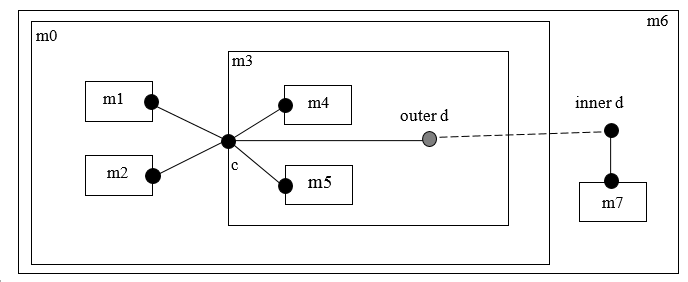
\includegraphics{innerouterconnector}
  \end{center}
  \caption{Example for inside and outside connectors.}
\end{figure}
The figure visualizes the following \lstinline!connect! equations to
the connector \lstinline!c! in the models \lstinline!m!$i$. Consider the
following \lstinline!connect! equations found in the model for component \lstinline!m0!:
\begin{lstlisting}[language=modelica]
connect(m1.c, m3.c); // m1.c and m3.c are inside connectors
connect(m2.c, m3.c); // m2.c and m3.c are inside connectors
\end{lstlisting}
and in the model for component \lstinline!m3! (\lstinline!c.x! is a sub-connector inside
\lstinline!c!):
\begin{lstlisting}[language=modelica]
connect(c, m4.c); // c is an outside
connector, m4.c is an inside connector
connect(c.x, m5.c); // c.x is an outside
connector, m5.c is an inside connector
connect(c , d) ; // c is an outside  connector, d  is an outside connector
\end{lstlisting}
and in the model for component \lstinline!m6!:
\begin{lstlisting}[language=modelica]
connect(d, m7.c); // d is an outside connector, m7.c is an inside connector
\end{lstlisting}
\end{example}

\subsection{Expandable Connectors}\label{expandable-connectors}

If the \lstinline!expandable! qualifier is present on a connector definition, all
instances of that connector are referred to as expandable connectors.
Instances of connectors that do not possess this qualifier will be
referred to as non-expandable connectors.

Before generating connection equations non-parameter scalar variables and non-parameter array elements declared in expandable connectors are marked as only being
potentially present.  A non-parameter array element may be declared with array dimensions \lstinline!:! indicating that the size is unknown (note that the size of
such a dimension cannot be determined using \lstinline!size!, see \cref{array-dimension-and-size-functions}).  This applies to both variables of simple types,
and variables of structured types.

Then connections containing expandable connectors are elaborated:
\begin{itemize}
\item
  One connector in the connect equation must reference a declared
  component, and if the other connector is an undeclared element in a
  declared expandable connector it is handled as follows (elements that
  are only potentially present are not seen as declared):
  \begin{itemize}
  \item
    The expandable connector instance is automatically augmented with a
    new component having the used name and corresponding type.
  \item
    If the undeclared component is subscripted, an array variable is created, and a connection to the specific array element is performed.  Introducing elements in an array gives an array with at least the specified elements, other elements are either not created or have a default value (i.e.\ as if they were only potentially present, and the same note regarding the use of \lstinline!size! also applies here).
  \item
    If the variable on the other side of the connect-equation is \lstinline!input! or \lstinline!output! the new component will be either \lstinline!input! or \lstinline!output! to satisfy the restrictions in \cref{restrictions-of-connections-and-connectors} for a non-expandable connector.
    \begin{nonnormative}
    If the existing side refers to an inside connector (i.e.\ a connector of a component) the new variable will copy its causality, i.e.\ \lstinline!input! if \lstinline!input! and \lstinline!output! if \lstinline!output!, since the expandable connector must be an outside connector.
    \end{nonnormative}
    For an array the \lstinline!input!/\lstinline!output! property can be deduced separately for each array element.
  \end{itemize}

\item
  When two expandable connectors are connected, each is augmented with the variables that are only declared in the other expandable connector (the new variables are neither \lstinline!input! nor \lstinline!output!).  This is repeated until all connected expandable connector instances have matching variables.
  \begin{nonnormative}
  I.e.\ each of the connector instances is expanded to be the union of all connector variables.
  \end{nonnormative}

\item
  The variables introduced in the elaboration follow additional rules for generating connection sets (given in \cref{generation-of-connection-equations}).

\item
  If a variable appears as an \lstinline!input! in one expandable connector, it should appear as a non-\lstinline!input! in at least one other expandable connector instance in the same augmentation set.  An augmentation set is defined as the set of connected expandable connector instances that through the elaboration will have matching variables.
\begin{example}
\begin{lstlisting}[language=modelica]
expandable connector EngineBus
end EngineBus;

block Sensor
  RealOutput speed; // Output, i.e., non-input
end Sensor;
block Actuator
  RealInput speed; // Input
end Actuator;

model Engine
  EngineBus bus;
  Sensor sensor;
  Actuator actuator;
equation
  connect(bus.speed, sensor.speed); // provides the non-input from sensor.speed
  connect(bus.speed, actuator.speed);
end Engine;
\end{lstlisting}
\end{example}

\item
  All components in an expandable connector are seen as connector
  instances even if they are not declared as such.
  \begin{nonnormative}
  I.e.\ it is possible to connect to e.g.\ a \lstinline!Real! variable.
  \end{nonnormative}
\begin{example}
\begin{lstlisting}[language=modelica]
expandable connector EngineBus // has predefined signals
  import Modelica.Units.SI;
  SI.AngularVelocity speed;
  SI.Temperature T;
end EngineBus;

block Sensor
 RealOutput speed;
end Sensor;

model Engine
  EngineBus bus;
  Sensor sensor;
equation
  connect(bus.speed, sensor.speed);
  // connection to non-connector speed is possible
  // in expandable connectors
end Engine;
\end{lstlisting}
\end{example}

\item
  An expandable connector shall not contain a component declared with the
  prefix \lstinline!flow!, but may contain non-expandable connector components with
  \lstinline!flow! components.
\begin{example}
\begin{lstlisting}[language=modelica]
import Interfaces=Modelica.Electrical.Analog.Interfaces;
expandable connector ElectricalBus
  Interfaces.PositivePin p12, n12; // OK
  flow Modelica.Units.SI.Current i; // Error
end ElectricalBus;

model Battery
  Interfaces.PositivePin p42, n42;
  ElectricalBus bus;
equation
  connect(p42, bus.p42); // Adds new electrical pin
  connect(n42, bus.n42); // Adds another pin
end Battery;
\end{lstlisting}
\end{example}

\item
  expandable connectors can only be connected to other expandable connectors.
\end{itemize}

If a connect equation references a potentially present variable, or variable element, in an expandable connector the variable or variable element is marked as being present, and due to the
paragraphs above it is possible to deduce whether the bus variable shall be treated as input, or shall be treated as output in the connect equation.  That \lstinline!input! or \lstinline!output!
prefix is added if no \lstinline!input!/\lstinline!output! prefix is present on the declaration.

\begin{example}
\begin{lstlisting}[language=modelica]
expandable connector EmptyBus
end EmptyBus;

model Controller
  EmptyBus bus1;
  EmptyBus bus2;
  RealInput speed;
equation
  connect(speed, bus1.speed); // OK; only one undeclared and not subscripted.
  connect(bus1.pressure, bus2.pressure); // Error; both undeclared.
  connect(speed, bus2.speed[2]); // Introduces speed array (with element [2]).
end Controller;
\end{lstlisting}
\end{example}

An expandable connector array component for which \lstinline!size! is not defined (see \cref{array-dimension-and-size-functions}) is referred to as a \emph{sizeless array component}.  Such a
component shall not be used without subscripts, and the subscripts must slice the array so that the sizeless dimensions are removed.

\begin{example}
Valid and invalid uses of sizeless array components:
\begin{lstlisting}[language=modelica]
expandable connector EngineBus
end EngineBus;

block Sensor
  RealOutput speed;
end Sensor;

model Engine
  parameter Integer n = 1;
  EngineBus bus;
  Sensor sensor;
  RealOutput sensorSpeeds[:];
equation
  /* Comments below refer to the use of sizeless array bus.speed. */
  connect(bus.speed[n], sensor.speed) ; // OK; subscript to scalar component.
  connect(bus.speed, sensorSpeeds); // Error; missing subscripts.
public
  Real s[:] = bus.speed; // Error; missing subscripts.
  Real s[2] = bus.speed[{1, 3}]; // OK; subscript selects fixed size sub-array.
end Engine;
\end{lstlisting}
\end{example}

After this elaboration the expandable connectors are treated as normal
connector instances, and the connections as normal connections, and all
potentially present variables and array elements that are not actually
present are undefined. It is an error if there
are expressions referring to potentially present variables or array
elements that are not actually present or non-declared variables. This
elaboration implies that expandable connectors can be connected even if
they do not contain the same components.

\begin{nonnormative}
A tool may remove undefined variables in an expandable connector, or set them to the default value, e.g.\ zero for \lstinline!Real! variables.
\end{nonnormative}

\begin{nonnormative}
Expressions can only ``read'' variables from the bus that
are actually declared and present in the connector, in order that the
types of the variables can be determined in the local scope.
\end{nonnormative}

\begin{nonnormative}
Note that the introduction of variables, as described above, is
conceptual and does not necessarily impact the flattening hierarchy in
any way. Furthermore, it is important to note that these elaboration
rules must consider:
\begin{enumerate}
\item Expandable connectors nested hierarchically. This means that
both outside and inside connectors must be included at every level of
the hierarchy in this elaboration process.
\item When processing an expandable connector that possesses the
\lstinline!inner! scope qualifier, all outer instances must also be taken into
account during elaboration.
\end{enumerate}
\end{nonnormative}

\begin{example}
Engine system with sensors, controllers, actuator and plant that
exchange information via a bus (i.e.\ via expandable connectors):
\begin{lstlisting}[language=modelica]
import Modelica.Units.SI;
import Modelica.Blocks.Interfaces.RealInput;
// Plant Side
model SparkPlug
  RealInput spark_advance;
  ...
end SparkPlug;

expandable connector EngineBus
  // No minimal set
end EngineBus;

expandable connector CylinderBus
  Real spark_advance;
end CylinderBus;

model Cylinder
  CylinderBus cylinder_bus;
  SparkPlug spark_plug;
  ...
equation
  connect(spark_plug.spark_advance,
  cylinder_bus.spark_advance);
end Cylinder;

model I4
  EngineBus engine_bus;
  Modelica.Mechanics.Rotational.Sensors.SpeedSensor speed_sensor;
  Modelica.Thermal.HeatTransfer.Sensors.TemperatureSensor temp_sensor;
  parameter Integer nCylinder = 4 "Number of cylinders";
  Cylinder cylinder[nCylinder];
equation
  // adds engine_speed (as output)
  connect(speed_sensor.w, engine_bus.engine_speed);
  // adds engine_temp (as output)
  connect(temp_sensor.T, engine_bus.engine_temp);
  // adds cylinder_bus1 (a nested bus)
  for i in 1:nCylinder loop
    connect(cylinder[i].cylinder_bus,
    engine_bus.cylinder_bus[i]);
  end for;
end I4;
\end{lstlisting}
Due to the above connection, conceptually a connector consisting
of the union of all connectors is introduced.

The \lstinline!engine_bus! contains the following variable declarations:
\begin{lstlisting}[language=modelica]
RealOutput engine_speed;
RealOutput engine_temp;
CylinderBus cylinder_bus[1];
CylinderBus cylinder_bus[2];
CylinderBus cylinder_bus[3];
CylinderBus cylinder_bus[4];
\end{lstlisting}
\end{example}

\section{Generation of Connection Equations}\label{generation-of-connection-equations}

When generating connection equations, \lstinline!outer! elements are resolved to the
corresponding \lstinline!inner! elements in the instance hierarchy (see instance
hierarchy name lookup \cref{instance-hierarchy-name-lookup-of-inner-declarations}). The arguments to each \lstinline!connect!-equation are
resolved to two connector elements.

For every use of the \lstinline!connect!-equation
\begin{lstlisting}[language=modelica]
connect(a, b);
\end{lstlisting}
the primitive components of \lstinline!a! and \lstinline!b! form a connection set, together with an indication of whether they are from an inside or an outside connector.  The primitive elements are
of simple types or of types defined as \lstinline!operator record! (i.e.\ a component of an \lstinline!operator record! type is not split into sub-components).  The elements of the connection sets
are tuples of primitive variables together with an indication of inside or outside; if the same tuple belongs to two connection sets those two sets are merged, until every tuple is only present in
one set.  Composite connector types are broken down into primitive components.  The \lstinline!outer! components are handled by mapping the objects to the corresponding \lstinline!inner! components,
and the inside indication is not influenced.  The outer connectors are handled by mapping the objects to the corresponding inner connectors, and they are always treated as outside connectors.

\begin{nonnormative}
Rationale: The inside/outside as part of the connection sets
ensure that connections from different hierarchical levels are treated
separately. Connection sets are formed from the primitive elements and
not from the connectors; this handles connections to parts of
hierarchical connectors and also makes it easier to generate equations
directly from the connection sets. All variables in one connection set
will either be flow variables or non-flow variables due to restriction
on connect-equations. The mapping from an \lstinline!outer! to an \lstinline!inner!
element must occur before merging the sets in order to get one
zero-sum equation, and ensures that the equations for the \lstinline!outer!
elements are all given for one side of the connector, and the
\lstinline!inner! element can define the other side.
\end{nonnormative}

The following connection sets with just one member are also present (and
merged):
\begin{itemize}
\item
  Each primitive flow variable as inside connector.
\item
  Each flow variable \emph{added} during augmentation of expandable
  connectors, both as inside and as outside.
  \begin{nonnormative}
  Note that the flow variable is not directly in the expandable connector, but in a connector inside the expandable connector.
  \end{nonnormative}
\end{itemize}

\begin{nonnormative}
Rationale: If these variables are not connected they will
generate a set comprised only of this element, and thus they will be
implicitly set to zero (see below). If connected, this set will be
merged and adding this at the start has no impact.
\end{nonnormative}

Each connection set is used to generate equations for potential and flow
(zero-sum) variables of the form
\begin{itemize}
\item
$a_{1} = a_{2} = \ldots = a_{n}$ (neither flow nor stream variables)
\item
$z_{1} + z_{2} + (-z_{3}) + \ldots + z_{n} = \mathbf{0}$ (flow variables)
\end{itemize}

The bold-face $\mathbf{0}$ represents an array or scalar zero of
appropriate dimensions (i.e.\ the same size as $z$).

For an \lstinline!operator record! type this uses the operator \lstinline!'0'! -- which must be defined in the operator record -- and all of the flow variables for the \lstinline!operator record!
must be of the same \lstinline!operator record! type.  This implies that in order to have flow variables of an \lstinline!operator record! type the \lstinline!operator record! must define addition,
negation, and \lstinline!'0'!; and these operations should define an additive group.

In order to generate equations for flow variables (using the
\lstinline!flow! prefix), the sign used for the connector variable
$z_{i}$ above is +1 for inside connectors and -1 for outside
connectors ($z_{3}$ in the example above).

\begin{example}
Simple example:
\begin{lstlisting}[language=modelica]
model Circuit
  Ground ground;
  Load load;
  Resistor resistor;
equation
  connect(load.p , ground.p);
  connect(resistor.p, ground.p);
end Circuit;

model Load
  extends TwoPin;
  Resistor resistor;
equation
  connect(p, resistor.p);
  connect(resistor.n, n);
end Load;
\end{lstlisting}
The connection sets are before merging (note that one part of the load and resistor is not connected):

\{\textless{}\lstinline!load.p.i!, inside\textgreater{}\}\\
\{\textless{}\lstinline!load.n.i!, inside\textgreater{}\}\\
\{\textless{}\lstinline!ground.p.i!, inside\textgreater{}\}\\
\{\textless{}\lstinline!load.resistor.p.i!, inside\textgreater{}\}\\
\{\textless{}\lstinline!load.resistor.n.i!, inside\textgreater{}\}\\
\{\textless{}\lstinline!resistor.p.i!, inside\textgreater{}\}\\
\{\textless{}\lstinline!resistor.n.i!, inside\textgreater{}\}\\
\{\textless{}\lstinline!resistor.p.i!, inside\textgreater{}, \textless{}\lstinline!ground.p.i!, inside\textgreater{}\}\\
\{\textless{}\lstinline!resistor.p.v!, inside\textgreater{}, \textless{}\lstinline!ground.p.v!, inside\textgreater{}\}\\
\{\textless{}\lstinline!load.p.i!, inside\textgreater{}, \textless{}\lstinline!ground.p.i!, inside\textgreater{}\}\\
\{\textless{}\lstinline!load.p.v!, inside\textgreater{}, \textless{}\lstinline!ground.p.v!, inside\textgreater{}\}\\
\{\textless{}\lstinline!load.p.i!, outside\textgreater{}, \textless{}\lstinline!load.resistor.p.i!, inside\textgreater{}\}\\
\{\textless{}\lstinline!load.p.v!, outside\textgreater{}, \textless{}\lstinline!load.resistor.p.v!, inside\textgreater{}\}\\
\{\textless{}\lstinline!load.n.i!, outside\textgreater{}, \textless{}\lstinline!load.resistor.n.i!, inside\textgreater{}\}\\
\{\textless{}\lstinline!load.n.v!, outside\textgreater{}, \textless{}\lstinline!load.resistor.n.v!, inside\textgreater{}\}

After merging this gives:

\{\textless{}\lstinline!load.p.i!, outside\textgreater{}, \textless{}\lstinline!load.resistor.p.i!, inside\textgreater{}\}\\
\{\textless{}\lstinline!load.p.v!, outside\textgreater{}, \textless{}\lstinline!load.resistor.p.v!, inside\textgreater{}\}\\
\{\textless{}\lstinline!load.n.i!, outside\textgreater{}, \textless{}\lstinline!load.resistor.n.i!, inside\textgreater{}\}\\
\{\textless{}\lstinline!load.n.v!, outside\textgreater{}, \textless{}\lstinline!load.resistor.n.v!, inside\textgreater{}\}\\
\{\textless{}\lstinline!load.p.i!, inside\textgreater{}, \textless{}\lstinline!ground.p.i!, inside\textgreater{}, \textless{}\lstinline!resistor.p.i!, inside\textgreater{}\}\\
\{\textless{}\lstinline!load.p.v!, inside\textgreater{}, \textless{}\lstinline!ground.p.v!, inside\textgreater{}, \textless{}\lstinline!resistor.p.v!, inside\textgreater{}\}\\
\{\textless{}\lstinline!load.n.i!, inside\textgreater{}\}\\
\{\textless{}\lstinline!resistor.n.i!, inside\textgreater{}\}

And thus the equations:
\begin{lstlisting}[language=modelica]
load.p.v = load.resistor.p.v;
load.n.v = load.resistor.n.v;
load.p.v = ground.p.v;
load.p.v = resistor.p.v;
0 = (-load.p.i) + load.resistor.p.i;
0 = (-load.n.i) + load.resistor.n.i;
0 = load.p.i + ground.p.i + resistor.p.i;
0 = load.n.i;
0 = resistor.n.i;
\end{lstlisting}
\end{example}

\begin{example}
Outer component example:
\begin{lstlisting}[language=modelica]
model Circuit
  Ground ground;
  Load load;
  inner Resistor resistor;
equation
  connect(load.p, ground.p);
end Circuit;

model Load
  extends TwoPin;
  outer Resistor resistor;
equation
  connect(p, resistor.p);
  connect(resistor.n, n);
end Load;
\end{lstlisting}
The connection sets are before merging (note that one part of the load and resistor is not connected):

\{\textless{}\lstinline!load.p.i!, inside\textgreater{}\}\\
\{\textless{}\lstinline!load.n.i!, inside\textgreater{}\}\\
\{\textless{}\lstinline!ground.p.i!, inside\textgreater{}\}\\
\{\textless{}\lstinline!resistor.p.i!, inside\textgreater{}\}\\
\{\textless{}\lstinline!resistor.n.i!, inside\textgreater{}\}\\
\{\textless{}\lstinline!load.p.i!, inside\textgreater{}, \textless{}\lstinline!ground.p.i!, inside\textgreater{}\}\\
\{\textless{}\lstinline!load.p.v!, inside\textgreater{}, \textless{}\lstinline!ground.p.v!, inside\textgreater{}\}\\
\{\textless{}\lstinline!load.p.i!, outside\textgreater{}, \textless{}\lstinline!resistor.p.i!, inside\textgreater{}\}\\
\{\textless{}\lstinline!load.p.v!, outside\textgreater{}, \textless{}\lstinline!resistor.p.v!, inside\textgreater{}\}\\
\{\textless{}\lstinline!load.n.i!, outside\textgreater{}, \textless{}\lstinline!resistor.n.i!, inside\textgreater{}\}\\
\{\textless{}\lstinline!load.n.v!, outside\textgreater{}, \textless{}\lstinline!resistor.n.v!, inside\textgreater{}\}

After merging this gives:

\{\textless{}\lstinline!load.p.i!, outside\textgreater{}, \textless{}\lstinline!resistor.p.i!, inside\textgreater{}\}\\
\{\textless{}\lstinline!load.p.v!, outside\textgreater{}, \textless{}\lstinline!resistor.p.v!, inside\textgreater{}\}\\
\{\textless{}\lstinline!load.n.i!, outside\textgreater{}, \textless{}\lstinline!resistor.n.i!, inside\textgreater{}\}\\
\{\textless{}\lstinline!load.n.v!, outside\textgreater{}, \textless{}\lstinline!resistor.n.v!, inside\textgreater{}\}\\
\{\textless{}\lstinline!load.p.i!, inside\textgreater{}, \textless{}\lstinline!ground.p.i!, inside\textgreater{}\}\\
\{\textless{}\lstinline!load.p.v!, inside\textgreater{}, \textless{}\lstinline!ground.p.v!, inside\textgreater{}\}\\
\{\textless{}\lstinline!load.n.i!, inside\textgreater{}\}

And thus the equations:
\begin{lstlisting}[language=modelica]
load.p.v = resistor.p.v;
load.n.v = resistor.n.v;
load.p.v = ground.p.v;
0 = (-load.p.i) + resistor.p.i;
0 = (-load.n.i) + resistor.n.i;
0 = load.p.i + ground.p.i;
0 = load.n.i;
\end{lstlisting}

This corresponds to a direct connection of the resistor.
\end{example}

\section{Restrictions of Connections and Connectors}\label{restrictions-of-connections-and-connectors}

\begin{itemize}
\item
  The connect-equations (and the special functions for overdetermined
  connectors) can only be used in equations and shall not be used inside
  if-equations with non-parametric condition, or in when-equations.
  \begin{nonnormative}
  For-equations always have parameter expressions for the array expression.
  \end{nonnormative}
\item
  A connector component shall not be declared with the prefix \lstinline!parameter! or \lstinline!constant!.  In the connect-equation the primitive components may only connect parameter variables to parameter variables and constant variables to constant variables.
\item
  The connect-equation construct only accepts forms of connector
  references as specified in \cref{connect-equations-and-connectors}.
\item
  In a connect-equation the two connectors must have the same named
  component elements with the same dimensions; recursively down to the
  primitive components. The primitive components with the same name are
  matched and belong to the same connection set.
\item
  The matched primitive components of the two connectors must have the same primitive types, and flow variables may only connect to other flow variables, stream variables only to other stream variables, and causal variables (\lstinline!input!/\lstinline!output!) only to causal variables (\lstinline!input!/\lstinline!output!).
\item
  A connection set of causal variables (\lstinline!input!/\lstinline!output!) may at most
  contain variables from one inside \lstinline!output! connector (for state-machines extended as specified in \cref{merging-connections-to-multiple-outputs}) or one public
  outside \lstinline!input! connector.
  \begin{nonnormative}
  I.e., a connection set may at most contain one source of a signal.
  \end{nonnormative}
\item
  At least one of the following must hold for a connection set
  containing causal variables generated for a non-partial model or
  block:
\begin{enumerate}
\item the connection set includes variables from an outside public
  expandable connector,
\item the set contains variables from protected
  outside connectors,
\item it contains variables from one inside \lstinline!output!
  connector, or
\item from one public outside \lstinline!input! connector, or
\item the  set is comprised solely of one variable from one inside \lstinline!input!
  connector that is not part of an expandable connector. \label{enum:exc-conn-case}
\end{enumerate}
\begin{nonnormative}
I.e., a connection set must -- unless the model or block is partial -- contain one source of a signal (\cref{enum:exc-conn-case}
covers the case where a connector of a component is left unconnected and the source given textually).
\end{nonnormative}
\item
  Variables from a protected outside connector must be part of a
  connection set containing at least one inside connector or one
  declared public outside connector (i.e.\ it shall not be an implicitly
  defined part of an expandable connector).
  \begin{nonnormative}
  Otherwise it would not be possible to deduce the causality for the expandable connector element.
  \end{nonnormative}
\item
  In a connection set all variables having non-empty quantity attribute
  must have the same quantity attribute.
\item
  A \lstinline!connect! equation shall not (directly or indirectly) connect two
  connectors of \lstinline!outer! elements.
  \begin{nonnormative}
  Indirectly is similar to them being part of the same connection set.  However, connections to \lstinline!outer! elements are ``moved up'' before forming
  connection sets.  Otherwise the connection sets could contain redundant information breaking the equation count for locally balanced models and blocks.
  \end{nonnormative}
\item
  Subscripts in a connector reference shall be parameter expressions or
  the special operator \lstinline!:!.
\item
  Constants or parameters in connected components yield the appropriate
  assert statements to check that they have the same value; connections
  are not generated.
\item
  For conditional connectors, see \cref{conditional-component-declaration}.
\end{itemize}

\subsection{Balancing Restriction and Size of Connectors}\label{balancing-restriction-and-size-of-connectors}

For each non-partial non-expandable connector class the number of flow variables shall
be equal to the number of variables that are neither \lstinline!parameter!,
\lstinline!constant!, \lstinline!input!, \lstinline!output!, \lstinline!stream!
nor \lstinline!flow!. The \emph{number of variables} is
the number of all elements in the connector class after expanding all
records and arrays to a set of scalars of primitive types. The number of
variables of an overdetermined type or record class (see \cref{overconstrained-equation-operators-for-connection-graphs})
is the size of the output argument of the corresponding
\lstinline!equalityConstraint!() function.
\begin{nonnormative}
Expandable connector classes are excluded from this, since their component declarations are only a form of constraint.
\end{nonnormative}

\begin{example}
\begin{lstlisting}[language=modelica]
connector Pin // a physical connector of
  Modelica.Electrical.Analog
  Real v;
  flow Real i;
end Pin;

connector Plug // a hierarchical connector of
  Modelica.Electrical.MultiPhase
  parameter Integer m=3;
  Pin p[m];
end Plug;

connector InputReal = input Real; // A causal input connector
connector OutputReal = output Real; // A causal output connector

connector Frame_Illegal
  Modelica.Units.SI.Position r0[3] "Position vector of frame origin";
  Real S[3, 3] "Rotation matrix of frame";
  Modelica.Units.SI.Velocity v[3] "Abs. velocity of frame origin";
  Modelica.Units.SI.AngularVelocity w[3] "Abs. angular velocity of frame";
  Modelica.Units.SI.Acceleration a[3] "Abs. acc. of frame origin";
  Modelica.Units.SI.AngularAcceleration z[3] "Abs. angular acc. of frame";
  flow Modelica.Units.SI.Force f[3] "Cut force";
  flow Modelica.Units.SI.Torque t[3] "Cut torque";
end Frame_Illegal;
\end{lstlisting}

The \lstinline!Frame_Illegal! connector (intended to be used in a simple multi-body package without over-determined connectors) is illegal since the number of flow and non-flow variables do not match. The solution is to create two connector classes, where two 3-vectors (e.g., \lstinline!a! and \lstinline!z!) are acausal \lstinline!Real! and the other variables are matching pairs of \lstinline!input! and \lstinline!output!.  This ensures that the models can only be connected in a tree-structure or require a ``loop-breaker'' joint for every closed kinematic loop:
\begin{lstlisting}[language=modelica]
connector Frame_a "correct connector"
  input Modelica.Units.SI.Position r0[3];
  input Real S[3, 3];
  input Modelica.Units.SI.Velocity v[3];
  input Modelica.Units.SI.AngularVelocity w[3];
  Modelica.Units.SI.Acceleration a[3];
  Modelica.Units.SI.AngularAcceleration z[3];
  flow Modelica.Units.SI.Force f[3];
  flow Modelica.Units.SI.Torque t[3];
end Frame_a;

connector Frame_b "correct connector"
  output Modelica.Units.SI.Position r0[3];
  output Real S[3, 3];
  output Modelica.Units.SI.Velocity v[3];
  output Modelica.Units.SI.AngularVelocity w[3];
  Modelica.Units.SI.Acceleration a[3];
  Modelica.Units.SI.AngularAcceleration z[3];
  flow Modelica.Units.SI.Force f[3];
  flow Modelica.Units.SI.Torque t[3];
end Frame_b;
\end{lstlisting}

The subsequent connectors \lstinline!Plug_Expanded! and \lstinline!PlugExpanded2!
are correct, but \lstinline!Plug_Expanded_Illegal! is illegal since
the number of non-flow and flow variables is different if \lstinline!n! and \lstinline!m! are different. It is not clear how a tool can detect in
general that connectors such as \lstinline!Plug_Expanded_Illegal! are
illegal. However, it is always possible to detect this defect after
actual values of parameters and constants are provided in the simulation
model.

\begin{lstlisting}[language=modelica]
connector Plug_Expanded "correct connector"
  parameter Integer m=3;
  Real v[m];
  flow Real i[m];
end Plug_Expanded;

connector Plug_Expanded2 "correct connector"
  parameter Integer m=3;
  final parameter Integer n=m;
  Real v[m];
  flow Real i[n];
end Plug_Expanded2;

connector Plug_Expanded_Illegal "connector is illegal"
  parameter Integer m=3;
  parameter Integer n=m;
  Real v[m];
  flow Real i[n];
end Plug_Expanded_Illegal;
\end{lstlisting}
\end{example}

\section{Equation Operators for Overconstrained Connection-Based Equation Systems}\label{equation-operators-for-overconstrained-connection-based-equation-systems1}

There is a special problem regarding equation systems resulting from
\emph{loops} in connection graphs where the connectors contain
\emph{non-flow} (i.e., potential) variables \emph{dependent} on each
other. When a loop structure occurs in such a graph, the resulting
equation system will be \emph{overconstrained}, i.e., have more
equations than variables, since there are implicit constraints between
certain non-flow variables in the connector in addition to the
connection equations around the loop. At the current state-of-the-art,
it is not possible to automatically eliminate the unneeded equations
from the resulting equation system without additional information from
the model designer.

This section describes a set of equation operators for such
overconstrained connection-based equation systems, that makes it
possible for the model designer to specify enough information in the
model to allow a Modelica environment to automatically remove the
superfluous equations.

\begin{nonnormative}
Connectors may contain redundant variables. For example, the
orientation between two coordinate systems in $3$ dimensions can be
described by $3$ independent variables. However, every description of
orientation with $3$ variables has at least one singularity in the region
where the variables are defined. It is therefore not possible to declare
only $3$ variables in a connector. Instead $n$ variables ($n > 3$) have to be used. These variables are no longer independent from each
other and there are $n - 3$ constraint equations that have to be fulfilled.
A proper description of a redundant set of variables with constraint
equations does no longer have a singularity. A model that has loops in
the connection structure formed by components and connectors with
redundant variables, may lead to a differential algebraic equation
system that has more equations than unknown variables. The superfluous
equations are usually consistent with the rest of the equations, i.e., a
unique mathematical solution exists. Such models cannot be treated with
the currently known symbolic transformation methods. To overcome this
situation, operators are defined in order that a Modelica translator can
remove the superfluous equations. This is performed by replacing the
equality equations of non-flow variables from connection sets by a
reduced number of equations in certain situations.

This section handles a certain class of overdetermined systems due
to connectors that have a redundant set of variables. There are other
causes of overdetermined systems, e.g., explicit zero-sum equations for
flow variables, that are not handled by the method described below.
\end{nonnormative}

\subsection{Overconstrained Equation Operators for Connection Graphs}\label{overconstrained-equation-operators-for-connection-graphs}

A type or record declaration may have an optional definition of function
\lstinline!equalityConstraint! that shall have the following prototype:
\begin{lstlisting}[language=modelica]
type Type // overdetermined type
  extends <base type>;
  function equalityConstraint // non-redundant equality
    input Type T1;
    input Type T2;
    output Real residue[ <n> ];
  algorithm
    residue := ...
  end equalityConstraint;
end Type;

record Record
  < declaration of record fields>
  function equalityConstraint // non-redundant equality
    input Record R1;
    input Record R2;
    output Real residue[ <n> ];
  algorithm
    residue := ...
  end equalityConstraint;
end Record;
\end{lstlisting}
The \lstinline!residue! output of the \lstinline!equalityConstraint! function shall have known size, say constant $n$.  The function shall express the equality between the two type instances \lstinline!T1! and \lstinline!T2! or the record instances \lstinline!R1! and \lstinline!R2!, respectively, with a non-redundant number $n \ge 0$ of equations.  The residues of these equations are returned in vector \lstinline!residue! of size $n$.  The set of $n$ non-redundant equations stating that \lstinline!R1 = R2! is given by the equation (\lstinline!0! represents a vector of zeros of appropriate size):
\begin{lstlisting}[language=modelica]
  Record R1, R2;
equation
  0 = Record.equalityConstraint(R1, R2);
\end{lstlisting}
\begin{nonnormative}
If the elements of a record \lstinline!Record! are not independent from each other, the equation \lstinline!R1 = R2! contains redundant equations.
\end{nonnormative}

A type class with an \lstinline!equalityConstraint! function declaration is called \firstuse{overdetermined type}.  A record class with an \lstinline!equalityConstraint! function definition is called
\firstuse{overdetermined record}.  A connector that contains instances of overdetermined type and/or record classes is called overdetermined connector.  An overdetermined type or record may neither
have flow components nor may be used as a type of flow components.  If an array is used as argument to any of the \lstinline!Connections.*! functions it is treated as one unit -- unlike
\lstinline!connect!, there is no special treatment of this case, compare \cref{connect-equations-and-connectors}.

Every instance of an overdetermined type or record in an overdetermined
connector is a node in a virtual connection graph that is used to
determine when the standard equation \lstinline!R1 = R2! or when the equation
\lstinline!0 = equalityConstraint(R1, R2)! has to be used for the generation of
\lstinline!connect! equations. The edges of the virtual connection graph are
implicitly defined by \lstinline!connect! and explicitly by
\lstinline!Connections.branch! statements, see table below. \lstinline!Connections! is a
built-in package in global scope containing built-in operators.
Additionally, corresponding nodes of the virtual connection graph have
to be defined as roots or as potential roots with functions
\lstinline!Connections.root! and \lstinline!Connections.potentialRoot!, respectively.

The overconstrained equation operators for connection graphs are listed below.  Here, \lstinline!A! and \lstinline!B! are connector instances that may be hierarchically structured, e.g., \lstinline!A! may be an abbreviation for \lstinline!EnginePort.Frame!.
\begin{center}
\begin{tabular}{l|l l}
\hline
\tablehead{Expression} & \tablehead{Description} & \tablehead{Details}\\
\hline
\hline
\lstinline!connect(A, B)! & Optional spanning-tree edge & \Cref{modelica:optional-spanning-tree-edge}\\
\lstinline!Connections.branch(A.R, B.R)! & Required spanning-tree edge & \Cref{modelica:Connections.branch}\\
\lstinline!Connections.root(A.R)! & Definite root node & \Cref{modelica:Connections.root}\\
\lstinline!Connections.potentialRoot(A.R, $\ldots$)! & Potential root node & \Cref{modelica:Connections.potentialRoot}\\
\lstinline!Connections.isRoot(A.R)! & Predicate for being selected as root & \Cref{modelica:Connections.isRoot}\\
\lstinline!Connections.rooted(A.R)! & Predicate for being closer to root & \Cref{modelica:Connections.rooted}\\
\hline
\end{tabular}
\end{center}

\begin{operatordefinition*}[connect]\label{modelica:optional-spanning-tree-edge}
\begin{synopsis}\begin{lstlisting}
connect(A, B)
\end{lstlisting}\end{synopsis}
\begin{semantics}
Defines \firstuse{optional spanning-tree edge} from the overdetermined type or record instances in connector instance \lstinline!A! to the corresponding overdetermined type or record instances in connector instance \lstinline!B! for a virtual connection graph.  The types of the corresponding overdetermined type or record instances shall be the same.
\end{semantics}
\end{operatordefinition*}

\begin{operatordefinition}[Connections.branch]
\begin{synopsis}\begin{lstlisting}
Connections.branch(A.R, B.R)
\end{lstlisting}\end{synopsis}
\begin{semantics}
Defines a \firstuse{required spanning-tree edge} from the overdetermined type or record instance \lstinline!R! in connector instance \lstinline!A! to the corresponding overdetermined type or record instance \lstinline!R! in connector instance \lstinline!B! for a virtual connection graph.  This function can be used at all places where a \lstinline!connect! statement is allowed.

\begin{nonnormative}
E.g., it is not allowed to use this function in a when-clause.  This definition shall be used if in a model with connectors \lstinline!A! and \lstinline!B! the overdetermined records \lstinline!A.R! and \lstinline!B.R! are algebraically coupled in the model, e.g., due to \lstinline!B.R = f(A.R!, \textless{}other unknowns\textgreater{}).
\end{nonnormative}
\end{semantics}
\end{operatordefinition}

\begin{operatordefinition}[Connections.root]
\begin{synopsis}\begin{lstlisting}
Connections.root(A.R)
\end{lstlisting}\end{synopsis}
\begin{semantics}
The overdetermined type or record instance \lstinline!R! in connector instance \lstinline!A! is a (definite) \firstuse{root node} in a virtual connection graph.

\begin{nonnormative}
This definition shall be used if in a model with connector \lstinline!A! the overdetermined record \lstinline!A.R! is (consistently) assigned, e.g., from a parameter expressions.
\end{nonnormative}
\end{semantics}
\end{operatordefinition}

\begin{operatordefinition}[Connections.potentialRoot]
\begin{synopsis}\begin{lstlisting}
Connections.potentialRoot(A.R)
Connections.potentialRoot(A.R, priority=$p$)
\end{lstlisting}\end{synopsis}
\begin{semantics}
The overdetermined type or record instance \lstinline!R! in connector instance \lstinline!A! is a \firstuse{potential root node} in a virtual connection graph with priority \lstinline!p! ($p \geq 0$). If no second argument is provided, the priority is zero. \lstinline!p! shall be a parameter expression of type \lstinline!Integer!.  In a virtual connection subgraph without a \lstinline!Connections.root! definition, one of the potential roots with the lowest priority number is selected as root.

\begin{nonnormative}
This definition may be used if in a model with connector \lstinline!A! the overdetermined record \lstinline!A.R! appears differentiated -- \lstinline!der(A.R)! -- together with the \emph{constraint equations} of \lstinline!A.R!, i.e., a non-redundant subset of \lstinline!A.R! maybe used as states.
\end{nonnormative}
\end{semantics}
\end{operatordefinition}

\begin{operatordefinition}[Connections.isRoot]
\begin{synopsis}\begin{lstlisting}
Connections.isRoot(A.R)
\end{lstlisting}\end{synopsis}
\begin{semantics}
Returns true, if the overdetermined type or record instance \lstinline!R! in connector instance \lstinline!A! is selected as a root in the virtual connection graph.
\end{semantics}
\end{operatordefinition}

\begin{operatordefinition}[Connections.rooted]
\begin{synopsis}\begin{lstlisting}
Connections.rooted(A.R)
rooted(A.R) // deprecated!
\end{lstlisting}\end{synopsis}
\begin{semantics}
If the operator \lstinline!Connections.rooted(A.R)! is used, or the equivalent but deprecated operator \lstinline!rooted(A.R)!, then there must be exactly one statement \lstinline!Connections.branch(A.R, B.R)! involving \lstinline!A.R! (the argument of \lstinline!Connections.rooted! must be the first argument of \lstinline!Connections.branch!).  In that case \lstinline!Connections.rooted(A.R)! returns true, if \lstinline!A.R! is closer to the root of the spanning tree than \lstinline!B.R!; otherwise false is returned.

\begin{nonnormative}
This operator can be used to avoid equation systems by providing analytic inverses, see\linebreak[4] \lstinline!Modelica.Mechanics.MultiBody.Parts.FixedRotation!.
\end{nonnormative}
\end{semantics}
\end{operatordefinition}

\begin{nonnormative}
Note, that \lstinline!Connections.branch!, \lstinline!Connections.root!,
\lstinline!Connections.potentialRoot! do not generate equations. They only
generate nodes and edges in the virtual graph for analysis purposes.
\end{nonnormative}


\subsection{Converting the Connection Graph into Trees and Generating Connection Equations}\label{converting-the-connection-graph-into-trees-and-generating-connection-equations}

Before \lstinline!connect! equations are generated, the virtual connection
graph is transformed into a set of spanning trees by removing optional spanning tree edges
from the graph. This is performed in the following way:
\begin{enumerate}
\item
  Every root node defined via the \lstinline!Connections.root! statement is
  a definite root of one spanning tree.
\item
  The virtual connection graph may consist of sets of subgraphs that are
  not connected together. Every subgraph in this set shall have at least
  one root node or one potential root node in a simulation model. If a
  graph of this set does not contain any root node, then one potential
  root node in this subgraph that has the lowest priority number is
  selected to be the root of that subgraph. The selection can be
  inquired in a class with function \lstinline!Connections.isRoot!, see table
  above.
\item
  If there are n selected roots in a subgraph, then optional spanning-tree edges
  have to be removed such that the result shall be a set of n spanning
  trees with the selected root nodes as roots.
\end{enumerate}

After this analysis, the connection equations are generated in the
following way:
\begin{enumerate}
\item
  For every optional spanning-tree edge (i.e., a \lstinline!connect(A, B)!
  equation), in one of the spanning trees, the connection
  equations are generated according to \cref{generation-of-connection-equations}.
\item
  For every optional spanning-tree edge not in any of the spanning trees, the
  connection equations are generated according to \cref{generation-of-connection-equations}, except
  for overdetermined type or record instances R. Here the equations
  \lstinline!0 = R.equalityConstraint(A.R, B.R)! are generated instead
  of \lstinline!A.R = B.R!.
\end{enumerate}

\subsection{Examples of Overconstrained Connection Graphs}\label{examples-of-overconstrained-connection-graphs}

\begin{example}
\begin{figure}[H]
  \begin{center}
    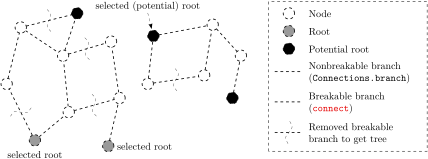
\includegraphics{overdetermined}
  \end{center}
  \caption{Example of a virtual connection graph.}
\end{figure}
\end{example}

\subsubsection{An Overdetermined Connector for Power Systems}\label{an-overdetermined-connector-for-power-systems}

\begin{nonnormative}
An overdetermined connector for power systems based on the
transformation theory of Park may be defined as:
\begin{lstlisting}[language=modelica]
type AC_Angle "Angle of source, e.g., rotor of generator"
  extends Modelica.Units.SI.Angle; // AC_Angle is a Real number
  // with unit = "rad"
  function equalityConstraint
    input AC_Angle theta1;
    input AC_Angle theta2;
    output Real residue[0] "No constraints";
  algorithm
    /* make sure that theta1 and theta2 from joining edges are identical */
    assert(abs(theta1 - theta2) < 1.e-10, "Consistent angles");
  end equalityConstraint;
end AC_Angle;

connector AC_Plug "3-phase alternating current connector"
  import Modelica.Units.SI;
  AC_Angle theta;
  SI.Voltage v[3] "Voltages resolved in AC_Angle frame";
  flow SI.Current i[3] "Currents resolved in AC_Angle frame";
end AC_Plug;
\end{lstlisting}
The currents and voltages in the connector are defined relatively
to the harmonic, high-frequency signal of a power source that is
essentially described by angle theta of the rotor of the source. This
allows much faster simulations, since the basic high frequency signal of
the power source is not part of the differential equations. For example,
when the source and the rest of the line operates with constant
frequency (= nominal case), then \lstinline!AC_Plug.v! and \lstinline!AC_Plug.i!
are constant. In this case a variable step integrator can select
large time steps. An element, such as a 3-phase inductor, may be
implemented as:
\begin{lstlisting}[language=modelica]
model AC_Inductor
  parameter Real X[3,3], Y[3,3]; // component constants
  AC_Plug p;
  AC_Plug n;
  Real omega;
equation
  Connections.branch(p.theta,n.theta); //edge in virtual graph
  // since n.theta = p.theta
  n.theta = p.theta; // pass angle theta between plugs
  omega = der (p.theta); // frequency of source
  zeros(3) = p.i + n.i;
  X*der (p.i) + omega*Y*p.i = p.v - n.v;
end AC_Inductor
\end{lstlisting}
At the place where the source frequency, i.e., essentially
variable theta, is defined, a \lstinline!Connections.root! must be present:
\begin{lstlisting}[language=modelica]
  AC_Plug p;
equation
  Connections.root(p.theta);
  der(p.theta) = 2*Modelica.Constants.pi*50 // 50 Hz;
\end{lstlisting}
The graph analysis performed with the virtual connection graph
identifies the connectors, where the \lstinline!AC_Angle! needs not to be
passed between components, in order to avoid redundant equations.
\end{nonnormative}

\subsubsection{An Overdetermined Connector for 3-dimensional Mechanical Systems}\label{an-overdetermined-connector-for-3-dimensional-mechanical-systems}

\begin{nonnormative}
An overdetermined connector for 3-dimensional mechanical systems
may be defined as:
\begin{lstlisting}[language=modelica]
type TransformationMatrix = Real[3,3];
type Orientation "Orientation from frame 1 to frame 2"
  extendsTransformationMatrix;
  function equalityConstraint
    input Orientation R1 "Rotation from inertial frame to frame 1";
    input Orientation R2 "Rotation from inertial frame to frame 2";
    output Real residue[3];
    protected
    Orientation R_rel "Relative Rotation from frame 1 to frame 2";
  algorithm
    R_rel := R2*transpose(R1);
    /*
      If frame_1 and frame_2 are identical, R_rel must be
      the unit matrix. If they are close together, R_rel can be
      linearized yielding:
        R_rel = [ 1, phi3, -phi2;
        -phi3, 1, phi1;
        phi2, -phi1, 1 ];
      where phi1, phi2, phi3 are the small rotation angles around
      axis x, y, z of frame 1 to rotate frame 1 into frame 2.
      The atan2 is used to handle large rotation angles, but does not
      modify the result for small angles.
    */
    residue := { Modelica.Math.atan2(R_rel[2, 3], R_rel[1, 1]),
    Modelica.Math.atan2(R_rel[3, 1], R_rel[2, 2]),
    Modelica.Math.atan2(R_rel[1, 2], R_rel[3, 3])};
  end equalityConstraint;
end Orientation;

connector Frame "3-dimensional mechanical connector"
  import Modelica.Units.SI;
  SI.Position r[3] "Vector from inertial frame to Frame";
  Orientation R "Orientation from inertial frame to Frame";
  flow SI.Force f[3] "Cut-force resolved in Frame";
  flow SI.Torque t[3] "Cut-torque resolved in Frame";
end Frame;
\end{lstlisting}
A fixed translation from a frame \lstinline!A! to a frame \lstinline!B! may be defined as:
\begin{lstlisting}[language=modelica]
model FixedTranslation
  parameter Modelica.Units.SI.Position r[3];
  Frame frame_a, frame_b;
equation
  Connections.branch(frame_a.R, frame_b.R);
  frame_b.r = frame_a.r + transpose(frame_a.R)*r;
  frame_b.R = frame_a.R;
  zeros(3) = frame_a.f + frame_b.f;
  zeros(3) = frame_a.t + frame_b.t + cross(r, frame_b.f);
end FixedTranslation;
\end{lstlisting}
Since the transformation matrix \lstinline!frame_a.R! is algebraically
coupled with \lstinline!frame_b.R!, an edge in the virtual connection graph
has to be defined. At the inertial system, the orientation is
consistently initialized and therefore the orientation in the inertial
system connector has to be defined as root:
\begin{lstlisting}[language=modelica]
model InertialSystem
  Frame frame_b;
equation
  Connections.root(frame_b.R);
  frame_b.r = zeros(3);
  frame_b.R = identity(3);
end InertialSystem;
\end{lstlisting}
\end{nonnormative}


% Arrays
\chapter{Arrays}\doublelabel{arrays}

An array can be regarded as a collection of values, all of the same
type. Modelica arrays can be multidimensional and are ``rectangular,''
which in the case of matrices has the consequence that all rows in a
matrix have equal length, and all columns have equal length.

Each array has a certain dimensionality, i.e., number of dimensions. The
degenerate case of a scalar variable is not really an array, but can be
regarded as an array with zero dimensions. Vectors have one dimension,
matrices have two dimensions, etc. {[}\emph{So-called row vectors and
column vectors do not exist in Modelica and cannot be distinguished
since vectors have only one dimension. If distinguishing these is
desired, row matrices and column matrices are available, being the
corresponding two-dimensional entities. However, in practice this is
seldom needed since the usual matrix arithmetic and linear algebra
operations have been defined to give the expected behavior when
operating on Modelica vectors and matrices.}{]}

Modelica is a strongly typed language, which also applies to array
types. The number of dimensions of an array is fixed and cannot be
changed at run-time {[}\emph{in order to permit strong type checking and
efficient implementation.}{]} However, the sizes of array dimensions can
be computed at run-time, {[}\emph{allowing fairly generic array
manipulation code to be written as well as interfacing to standard
numeric libraries implemented in other programming languages}.{]}

An array is allocated by declaring an array variable or calling an array
constructor. Elements of an array can be indexed by \lstinline!Integer!, \lstinline!Boolean!, or
\lstinline!enumeration! values.

\section{Array Declarations}\doublelabel{array-declarations}

The Modelica type system includes scalar number, vector, matrix (number
of dimensions, ndim=2), and arrays of more than two dimensions.
{[}\emph{There is no distinguishing between a row and column vector}.{]}

The following table shows the two possible forms of declarations and
defines the terminology. C is a placeholder for any class, including the
built-in type classes Real, Integer, Boolean, String, and enumeration
types. The type of a dimension upper bound expression, e.g. n, m, p,...
in the table below, need to be a subtype of Integer or EB for a class EB
that is an enumeration type or subtype of the Boolean type. Colon (:)
indicates that the dimension upper bound is unknown and is a subtype of
Integer.

Upper and lower array dimension index bounds are described in \autoref{array-dimension-lower-and-upper-index-bounds}.

An array indexed by Boolean or enumeration type can only be used in the
following ways:

\begin{itemize}
\item
  Subscripted using expressions of the appropriate type (i.e. Boolean or
  the enumerated type)
\item
  Binding equations of the form \lstinline!x1 = x2! as well as declaration
  assignments of the form \lstinline!x1 := x2! are allowed for arrays independent of
  whether the index types of dimensions are subtypes of Integer,
  Boolean, or enumeration types.
\end{itemize}

% IMPROVETOP
\begin{longtable}{|l|l|l|l|p{4cm}|}
\caption{General forms of declaration of arrays.}\\
\hline
\emph{Modelica form 1} & \emph{Modelica form 2} & \emph{\# dimensions} & \emph{Designation} & \emph{Explanation}\\ \hline
\endhead
C x; & C x; & 0 & Scalar & Scalar\\ \hline
C{[}n{]} x; & C x{[}n{]}; & 1 & Vector & n -- Vector\\ \hline
C{[}EB{]} x; & C x{[}EB{]} & 1 & Vector & Vector index by enumeration or
Boolean type EB\\ \hline
C{[}n, m{]} x; & C x{[}n, m{]}; & 2 & Matrix & n x m
Matrix\\ \hline
C{[}$n_1$, $n_{2}$,\ldots{},$n_k${]} x; & C x{[}$n_1$, $n_2$,\ldots{},$n_k${]}; & k & Array & Array with k dimensions
(k\textgreater{}=0).\\ \hline
\end{longtable}

{[}\emph{The number of dimensions and the dimensions sizes are part of
the type, and shall be checked for example at redeclarations.
Declaration form 1 displays clearly the type of an array, whereas
declaration form 2 is the traditional way of array declarations in
languages such as Fortran, C, C++.}

\begin{lstlisting}[language=modelica]
  Real[:] v1, v2 // vectors v1 and v2 have unknown sizes. The actual sizes may be different.
\end{lstlisting}

\emph{It is possible to mix the two declaration forms although it might
be confusing.}

\begin{lstlisting}[language=modelica]
  Real[3,2] x[4,5]; // x has type Real[4,5,3,2];
\end{lstlisting}
\emph{The reason for this order is given by examples such as:}

\begin{lstlisting}[language=modelica]
  type R3=Real[3];
  R3 a;
  R3 b[1]={a};
  Real[3] c[1]=b;
\end{lstlisting}
\emph{Using a type for ``a'' and ``b'' in this way is normal, and
substituting a type by its definition allow ``c''.}

\emph{A vector y indexed by enumeration values}

\begin{lstlisting}[language=modelica]
  type TwoEnums = enumeration(one,two);
  Real[TwoEnums] y;
\end{lstlisting}
{]}

Zero-valued dimensions are allowed, so: \lstinline!C x[0];! declares an empty
  vector and: \lstinline!C x[0,3]!; an empty matrix.
{[}\emph{Special cases}:

\begin{longtable}{|l|l|l|l|p{3cm}|}
\caption{Declaration of arrays as 1-vectors, row-vectors, or
column-vectors of arrays.}\\
\hline
\emph{Modelica form 1} & \emph{Modelica form 2} & \emph{\# dimensions} &
\emph{Designation} & \emph{Explanation}\\ \hline
\endhead
C{[}1{]} x; & C x{[}1{]};  & 1 & Vector & 1 -- Vector, representing a scalar\\ \hline
C{[}1,1{]} x; & C x{[}1, 1{]}; & 2 & Matrix & 1 x 1 -- Matrix, representing a scalar\\ \hline
C{[}n,1{]} x; & C x{[}n, 1{]}; & 2 & Matrix & n x 1 -- Matrix, representing a column\\ \hline
C{[}1,n{]} x; & C x{[}1, n{]}; & 2 & Matrix & 1 x n -- Matrix, representing a row\\ \hline
\end{longtable}

{]}

The type of an array of array is the multidimensional array which is
constructed by taking the first dimensions from the component
declaration and subsequent dimensions from the maximally expanded
component type. A type is maximally expanded, if it is either one of the
built-in types (Real, Integer, Boolean, String, enumeration type) or it
is not a type class. Before operator overloading is applied, a type
class of a variable is maximally expanded.

{[}\emph{Example}:

\begin{lstlisting}[language=modelica]
  type Voltage = Real(unit = "V");
  type Current = Real(unit = "A");
  connector Pin
    Voltage v; // type class of v = Voltage, type of v = Real
    flow Current i; // type class of i = Current, type of i = Real
  end Pin;
  type MultiPin = Pin[5];
  MultiPin[4] p; // type class of p is MultiPin, type of p is Pin[4,5];
  type Point = Real[3];
  Point p1[10];
  Real p2[10,3];
\end{lstlisting}
  The components p1 and p2 have identical types.
\begin{lstlisting}[language=modelica]
  p2[5] = p1[2]+ p2[4]; // equivalent to p2[5,:] = p1[2,:] + p2[4,:]
  Real r[3] = p1[2]; // equivalent to r[3] = p1[2,:]
\end{lstlisting}
{]}

{[}\emph{Automatic assertions at simulation time}:

\emph{Let A be a declared array and i be the declared maximum dimension
size of the} \lstinline!di!\emph{-dimension, then an assert statement}
\lstinline!assert(i>=0, ...)! \emph{is generated provided this
assertion cannot be checked at compile time. It is a quality of
implementation issue to generate a good error message if the assertion
fails.}

\emph{Let A be a declared array and i be an index accessing an index of
the} \lstinline!di!\emph{-dimension. Then for every such index-access an assert
statement} \lstinline!assert(i>=1 and i<=size(A,di), ...!
\emph{) is generated, provided this assertion cannot be checked at
compile time.}

\emph{For efficiency reasons, these implicit assert statement may be
optionally suppressed.}{]}

\subsection{Array Dimension Lower and Upper Index Bounds}\doublelabel{array-dimension-lower-and-upper-index-bounds}

The lower and upper index bounds for a dimension of an array indexed by
\lstinline!Integer!, \lstinline!Boolean!, or \lstinline!enumeration! values are as follows:

\begin{itemize}
\item
  An array dimension indexed by integers has a lower bound of 1 and an
  upper bound being the size of the dimension.
\item
  An array dimension indexed by \lstinline!Boolean! values has the lower bound \lstinline!false!
  and the upper bound \lstinline!true!.
\item
  An array dimension indexed by \lstinline!enumeration! values of the type
  \lstinline!E=enumeration!(\lstinline!e1!, \lstinline!e2!, ..., \lstinline!en!) has the lower bound \lstinline!E.e1! and the upper
  bound \lstinline!E.en!.
\end{itemize}

\section{Flexible Array Sizes}\doublelabel{flexible-array-sizes}

Regarding flexible array sizes and resizing of arrays in functions, see
\autoref{flexible-array-sizes-and-resizing-of-arrays-in-functions}.

\section{Built-in Array Functions}\doublelabel{built-in-array-functions}

Modelica provides a number of built-in functions that are applicable to
arrays.

The following \lstinline!promote! function cannot be used in Modelica, but is
utilized below to define other array operators and functions:

\begin{longtable}[]{|l|p{9cm}|}
\caption{Promote function (cannot be used in Modelica).}\\
\hline \endhead
promote(A,n) & Fills dimensions of size 1 from the right to array A upto
dimension n, where "n \textgreater{}= ndims(A)" is required. Let C =
promote(A,n), with nA=ndims(A), then ndims(C) = n, size(C,j) = size(A,j)
for 1 \textless{}= j \textless{}= nA, size(C,j) = 1 for nA+1 <= j <= n, C{[}i\_1, ..., i\_nA, 1, ..., 1{]} =A{[}i\_1, ..., i\_nA{]}\\ \hline
\end{longtable}

{[}\emph{The function} \lstinline!promote! \emph{cannot be used in Modelica, because
the number of dimensions of the returned array cannot be determined at
compile time if n is a variable. Below,} \lstinline!promote! \emph{is only used for
constant n}.

\emph{Some examples of using the functions defined in the following
\autoref{array-dimension-and-size-functions} to \autoref{matrix-and-vector-algebra-functions}}:

\begin{lstlisting}[language=modelica]
  Real x[4,1,6];
  size(x,1) = 4;
  size(x); // vector with elements 4, 1, 6
  size(2*x+x ) = size(x);
  Real[3] v1 = fill(1.0, 3);
  Real[3,1] m = matrix(v1);
  Real[3] v2 = vector(m);
  Boolean check[3,4] = fill(true, 3, 4);
\end{lstlisting}
{]}

\subsection{Array Dimension and Size Functions}\doublelabel{array-dimension-and-size-functions}

The following built-in functions for array dimensions and dimension
sizes are provided:

\begin{longtable}[]{|l|p{9cm}|}
\caption{Built-in array dimension and size functions.}\\
\hline
\emph{Modelica} & \emph{Explanation}\\ \hline
\endhead
\lstinline!ndims(A)! & 
Returns the number of dimensions k of expression A, with k
\textgreater{}= 0.
\\ \hline
\lstinline!size(A,i)! &
Returns the size of dimension i of array expression A where i shall be
\textgreater{} 0 and \textless{}= ndims(A).\\ \hline
\lstinline!size(A)! &
Returns a vector of length ndims(A) containing the dimension sizes of
A.\\ \hline
\end{longtable}

\subsection{Dimensionality Conversion Functions}\doublelabel{dimensionality-conversion-functions}

The following built-in conversion functions convert scalars, vectors,
and arrays to scalars, vectors, or matrices by adding or removing
1-sized dimensions.

\begin{longtable}[]{|l|p{9cm}|}
\caption{Built-in dimensionality conversion functions.}\\
\hline
\emph{Modelica} & \emph{Explanation}\\ \hline
\endhead
\lstinline!scalar(A)! & Returns the single element of array A. size(A,i) = 1 is required for 1
\textless{}= i \textless{}= ndims(A).\\ \hline
\lstinline!vector(A)!
& 
Returns a 1-vector, if A is a scalar and otherwise returns a vector
containing all the elements of the array, provided there is at most one
dimension size \textgreater{} 1.\\ \hline
\lstinline!matrix(A)!
& 
Returns promote(A,2), if A is a scalar or vector and otherwise returns
the elements of the first two dimensions as a matrix. size(A,i) = 1 is
required for 2 \textless{} i \textless{}= ndims(A).\\ \hline
\end{longtable}

\subsection{Specialized Array Constructor Functions}\doublelabel{specialized-array-constructor-functions}

An array constructor function constructs and returns an array computed
from its arguments. Most of the constructor functions in the table below
construct an array by filling in values according to a certain pattern,
in several cases just giving all array elements the same value. The
general array constructor with syntax \lstinline!array! (\ldots{}) or \{\ldots{}\}
is described in \autoref{vector-matrix-and-array-constructors}.

\begin{longtable}[]{|l|p{11cm}|}
\caption{Specialized array constructor functions.}\\
\hline
\emph{Modelica} & \emph{Explanation}\\ \hline
\endhead
\lstinline!identity(n)!
&
Returns the n x n Integer identity matrix, with ones on the diagonal and
zeros at the other places.\\ \hline
\lstinline!diagonal(v)!
&
Returns a square matrix with the elements of vector v on the diagonal
and all other elements zero.\\ \hline
\texttt{zeros(n\textsubscript 1,n\textsubscript 2,n\textsubscript 3,...)} &
Returns the $n_1$ x $n_2$ x $n_3$ x ... Integer array with all elements equal to zero ($n_i$
\textgreater{}= 0). The function need one or more arguments, that is
zeros() is not legal.\\ \hline
\texttt{ones(n\textsubscript 1,n\textsubscript 2,n\textsubscript 3,...)} &
Return the $n_1$ x $n_2$ x $n_3$ x ... Integer array with all elements equal to one ($n_i$
\textgreater{}=0 ). The function need one or more arguments, that is
ones() is not legal.\\ \hline
\texttt{fill(s,n\textsubscript 1,n\textsubscript 2,n\textsubscript 3,...)} &
Returns the $n_1$ x $n_2$ x $n_3$ x ... array with all elements equal to scalar or array expression s
($n_i$ \textgreater{}= 0). The returned array has the same
type as s.
Recursive definition:
\lstinline!fill!(s,$n_1$,$n_2$,$n_3$,...) =
\lstinline!fill!(\lstinline!fill!(s,$n_2$,$n_3$, ...),
$n_1$,); \lstinline!fill!(s,n)=\{s,s,\ldots{}, s\}

The function needs two or more arguments; that is fill(s) is not
legal.\\ \hline
\lstinline!linspace(x1,x2,n)!
&
Returns a Real vector with n equally spaced elements, such that
v=\lstinline!linspace!(x1,x2,n),

\lstinline!v[i] = x1 + (x2-x1)*(i-1)/(n-1) for 1 <= i <= n!.
It is required that n \textgreater{}= 2. The arguments x1 and x2 shall
be numeric scalar expressions.\\ \hline
\end{longtable}

\subsection{Reduction Functions and Operators}\doublelabel{reduction-functions-and-operators}

A reduction function ``reduces'' an array (or several scalars) to one
value (normally a scalar - but the sum reduction function may give an
array as result and also be applied to an operator record). Note that
none of these operators (particularly min and max) generate events
themselves (but arguments could generate events). The restriction on the
type of the input in \autoref{reduction-expressions} for reduction expressions also
apply to the array elements/scalar inputs for the reduction operator
with the same name.

The sum reduction function (both variants) may be applied to an operator
record, provided that the operator record defines '0' and '+'. It is
then assumed to form an additive group.

The following reduction functions are available:

\begin{longtable}{|p{4.1cm}|p{10.1cm}|}
\caption{Array reduction functions and operators.}\\
\hline
\emph{Modelica} & \emph{Explanation}\\ \hline
\endhead
\lstinline!min(A)!
&
Returns the least element of array expression A; as defined by
\textless{}.\\ \hline
\lstinline!min(x,y)!
&
Returns the least element of the scalars x and y; as defined by
\textless{}.\\ \hline
\begin{tabular}{@{}p{4cm}@{}}
\lstinline!min(e(i, ..., j)!\\
\lstinline! for i in  u,!\\
\lstinline!   ...,  j in  v)!
\end{tabular}
&
\begin{tabular}{@{}p{10cm}@{}}
Also described in \autoref{reduction-expressions}\\
Returns the least value (as defined by \textless{}) of the scalar
expression e(i, ..., j) evaluated for all combinations of i in u, ..., j
in v:
\end{tabular}\\ \hline
\lstinline!max(A)!
&
Returns the greatest element of array expression A; as defined by
\textgreater{}.\\ \hline
\lstinline!max(x,y)!
&
Returns the greatest element of the scalars x and y; as defined by
\textgreater{}.\\ \hline
\begin{tabular}{@{}p{4cm}@{}}
\lstinline!max(e(i, ..., j)!\\
\lstinline! for i in  u,!\\
\lstinline!   ...,  j in  v)!
\end{tabular}
&
\begin{tabular}{@{}p{10cm}@{}}
Also described in \autoref{reduction-expressions}
Returns the greatest value (as defined by \textgreater{}) of the scalar
expression e(i, ..., j) evaluated for all combinations of i in u, ..., j
in v:
\end{tabular}\\ \hline
\lstinline!sum(A)!
&
\begin{tabular}{@{}p{10cm}@{}}
Returns the scalar sum of all the elements of array expression:\\
\lstinline!=sum(A[j,k,...]) for j,k,...!
\end{tabular}\\ \hline
\begin{tabular}{@{}p{5cm}@{}}
\lstinline!sum(e(i, ..., j)!\\
\lstinline! for i in  u,!\\
\lstinline!   ...,  j in  v)!
\end{tabular}
&
\begin{tabular}{@{}p{10cm}@{}}
Also described in \autoref{reduction-expressions}\\
Returns the sum of the expression e(i, ..., j) evaluated for all
combinations of i in u, ..., j in v: For \lstinline!Integer! indexing this is
  e(u{[}1{]},...
  ,v{[}1{]})+e(u{[}2{]},... ,v{[}1{]})+... +e(u{[}end{]},...
  ,v{[}1{]})+...+e(u{[}end{]},... ,v{[}end{]})
  For non-\lstinline!Integer! this uses all valid indices instead of 1..end.
  The type of sum(e(i, ..., j) for  i in u, ..., j
    in v) is the same as the type of e(i,...j).
\end{tabular}\\ \hline
\lstinline!product(A)!
&
\begin{tabular}{@{}p{10cm}@{}}
Returns the scalar product of all the elements of array expression A.\\
  \lstinline!=product(A[j,k,...] for j,k,...!
\end{tabular}\\ \hline
\begin{tabular}{@{}p{4cm}@{}}
\lstinline!product(e(i, ..., j)!\\
\lstinline! for i in  u,!\\
\lstinline!   ...,  j in  v)!
\end{tabular}
&
\begin{tabular}{@{}p{10cm}@{}}
Also described in \autoref{reduction-expressions}.\\
Returns the product of the scalar expression e(i, ..., j) evaluated for
all combinations of i in u, ..., j in v: For \lstinline!Integer! indexing this is
\begin{lstlisting}[language=modelica]
  e(u[1],...,v[1])*e(u[2],...,v[1])*...
  *(u[end],...,v[1])*...*e(u[end],...,v[end])
\end{lstlisting}
  For non-\lstinline!Integer! this uses all valid indices instead of 1..end.
  The type of product(e(i, ..., j) for  i in u, ..., j
    in v) is the same as the type of e(i,...j).
\end{tabular}
\\ \hline
\end{longtable}

\subsubsection{Reduction Expressions}\doublelabel{reduction-expressions}

An expression:
\begin{lstlisting}[language=grammar]
function-name "(" expression1 for iterators ")"
\end{lstlisting}

is a reduction-expression. The expressions in the iterators of a
reduction-expression shall be vector expressions. They are evaluated
once for each reduction-expression, and are evaluated in the scope
immediately enclosing the reduction-expression.

For an iterator:
\begin{lstlisting}[language=grammar]
IDENT in expression2
\end{lstlisting}

the loop-variable, \lstinline!IDENT!, is in scope inside \lstinline!expression1!. The
loop-variable may hide other variables, as in for-clauses. The result
depends on the \lstinline!function-name!, and currently the only legal
function-names are the built-in operators \lstinline!array!, \lstinline!sum!,
\lstinline!product!, \lstinline!min!, and
\lstinline!max!. For array, see \autoref{vector-matrix-and-array-constructors}. If \lstinline!function-name! is
\lstinline!sum!, \lstinline!product!, \lstinline!min!,
or \lstinline!max! the result is of the same type as \lstinline!expression1! and is constructed
by evaluating \lstinline!expression1! for each value of the loop-variable and
computing the \lstinline!sum!, \lstinline!product!, \lstinline!min!, or
\lstinline!max! of the computed elements. For
deduction of ranges, see \autoref{implicit-iteration-ranges}; and for using types as ranges
see \autoref{types-as-iteration-ranges}.

\begin{longtable}{|p{3cm}|p{5cm}|p{6cm}|}
\caption{Reduction expressions with iterators.}\\
\hline
\emph{Function-name} & \emph{Restriction on expression1} & \emph{Result if expression2 is empty}\\ \hline
\endhead
\lstinline!sum! & Integer or Real & \lstinline!zeros(...)!\\ \hline
\lstinline!product! & Scalar Integer or Real & \lstinline!1!\\ \hline
\lstinline!min! & Scalar enumeration, Boolean, Integer or Real & 
\begin{tabular}{@{}p{6cm}@{}}
Greatest value of type\\( \lstinline!Modelica.Constants.inf! for Real)
\end{tabular}\\ \hline
\lstinline!max! & Scalar enumeration, Boolean, Integer or Real &
\begin{tabular}{@{}p{6cm}@{}}
Least value of type\\ ( \lstinline!-Modelica.Constants.inf! for Real)
\end{tabular}\\ \hline

\end{longtable}

{[}\emph{Example}:

% No frame since the math would break it.
\begin{lstlisting}[language=modelica, mathescape=true, frame=none]
  sum(i for  i in 1:10) // Gives $\sum_{i=1}^{10}i=$1+2+...+10=55
  // Read it as: compute the sum of i for i in the range 1 to 10.
  sum(i^2 for  i in {1,3,7,6}) // Gives $\sum_{i\in \begin{Bmatrix}1&3&7&6\end{Bmatrix}}i^2=$1+9+49+36=95
  {product(j for j in 1:i) for i in 0:4} // Gives {1,1,2,6,24}
  max(i^2 for  i in {3,7,6}) // Gives 49
\end{lstlisting}
{]}

\subsection{Matrix and Vector Algebra Functions}\doublelabel{matrix-and-vector-algebra-functions}

The following set of built-in matrix and vector algebra functions are
available. The function transpose can be applied to any matrix. The
functions outerProduct, symmetric, cross and skew require Real/Integer
vector(s) or matrix as input(s) and returns a Real vector or matrix:

\begin{longtable}[]{|p{3.5cm}|p{11.5cm}|}
\caption{Matrix and vector algebra functions.}\\
\hline
\emph{Modelica} & \emph{Explanation}\\ \hline
\endhead
\lstinline!transpose(A)!
& Permutes the first two dimensions of array A. It is an error, if array A
does not have at least 2 dimensions.\\ \hline
\lstinline!outerProduct(v1,v2)!
& Returns the outer product of vectors v1 and v2 ( = matrix(v1)*transpose(
matrix(v2) ) ).\\ \hline
\lstinline!symmetric(A)!
& Returns a matrix where the diagonal elements and the elements above the
diagonal are identical to the corresponding elements of matrix A and
where the elements below the diagonal are set equal to the elements
above the diagonal of A, i.e., \lstinline!B := symmetric(A) ->!
  \lstinline!B[i,j] := A[i,j], if i <= j, ! \lstinline! B[i,j] := A[j,i], if i > j!.\\ \hline
\lstinline!cross(x,y)!
& Returns the cross product of the 3-vectors x and y, i.e.
\lstinline!cross(x,y) = vector( [ x[2]*y[3]-x[3]*y[2];  x[3]*y[1]-x[1]*y[3]; x[1]*y[2]-x[2]*y[1]  ] );!\\ \hline
\lstinline!skew(x)!
& Returns the 3 x 3 skew symmetric matrix associated with a 3-vector,
  i.e., \lstinline!cross(x,y) = skew(x)*y; skew(x) = [0, -x[3], x[2]; x[3], 0, -x[1]; -x[2], x[1], 0];!\\ \hline
\end{longtable}

\section{Vector, Matrix and Array Constructors}\doublelabel{vector-matrix-and-array-constructors}

The constructor function \lstinline!array(A,B,C,...)! constructs an array from its
arguments according to the following rules:

\begin{itemize}
\item
  Size matching: All arguments must have the same sizes, i.e.,
  \lstinline!size(A)=size(B)=size(C)=!...
\item
  All arguments must be type compatible expressions (\autoref{type-compatible-expressions}) giving
  the type of the elements. The data type of the result array is the
  maximally expanded type of the arguments. Real and Integer subtypes
  can be mixed resulting in a Real result array where the Integer
  numbers have been transformed to Real numbers.
\item
  Each application of this constructor function adds a one-sized
  dimension to the left in the result compared to the dimensions of the
  argument arrays, i.e., \lstinline!ndims(array(A,B,C)) = ndims(A) + 1 = ndims(B) + 1, ...!
\item
  \lstinline!{A, B, C, ...}! is a shorthand notation for \lstinline!array(A, B, C, ...)!.
\item
  There must be at least one argument {[}\emph{i.e.,} \lstinline!array()! \emph{or}
  \lstinline!{}! \emph{is not defined}{]}.
\end{itemize}

{[}\emph{Examples}:
\begin{lstlisting}[language=modelica, escapechar=!]
  {1,2,3} !\emph{is a 3-vector of type Integer}.!
  {{11,12,13}, {21,22,23}} !\emph{is a 2x3 matrix of type Integer}!
  {{{1.0, 2.0, 3.0}}} !\emph{is a 1x1x3 array of type Real}.!

  Real[3] v = array(1, 2, 3.0);
  type Angle = Real(unit="rad");
  parameter Angle alpha = 2.0; // type of alpha is Real.
  // array(alpha, 2, 3.0) or {alpha, 2, 3.0} is a 3-vector of type Real.
  Angle[3] a = {1.0, alpha, 4}; // type of a is Real[3].
\end{lstlisting}
{]}

\subsection{Array Constructor with Iterators}\doublelabel{array-constructor-with-iterators}

An expression:
\begin{lstlisting}[language=grammar]
"{" expression for iterators "}"
\end{lstlisting}
or
\begin{lstlisting}[language=grammar]
array "(" expression for iterators ")"
\end{lstlisting}

is an array constructor with iterators. The expressions inside the
iterators of an array constructor shall be vector expressions. They are
evaluated once for each array constructor, and are evaluated in the
scope immediately enclosing the array constructor.

For an iterator:
\begin{lstlisting}[language=modelica]
IDENT in array_expression
\end{lstlisting}

the loop-variable, \lstinline!IDENT!, is in scope inside expression in the array
construction. The loop-variable may hide other variables, as in
for-clauses. The loop-variable has the same type as the type of the
elements of array\_expression; and can be simple type as well as a
record type. The loop-variable will have the same type for the entire
loop - i.e. for an array\_expression \{1,3.2\} the iterator will have
the type of the type-compatible expression (Real) for all iterations.
For deduction of ranges, see \autoref{implicit-iteration-ranges}; and for using types as
range see \autoref{types-as-iteration-ranges}.

\subsubsection{Array Constructor with One Iterator}\doublelabel{array-constructor-with-one-iterator}

If only one iterator is used, the result is a vector constructed by
evaluating expression for each value of the loop-variable and forming an
array of the result.

{[}\emph{Example}:
\begin{lstlisting}[language=modelica]
array(i for i in 1:10)
// Gives the vector 1:10={1,2,3,...,10} 
 
{r for r in 1.0 : 1.5 : 5.5} 
// Gives the vector 1.0:1.5:5.5={1.0, 2.5, 4.0, 5.5} 
 
{i^2 for i in {1,3,7,6}} 
// Gives the vector {1, 9, 49, 36}
\end{lstlisting}
\subsubsection{Array Constructor with Several Iterators}\doublelabel{array-constructor-with-several-iterators}

The notation with several iterators is a shorthand notation for nested
array constructors. The notation can be expanded into the usual form by
replacing each '\lstinline!,!' by '\lstinline!} for!' and prepending the array constructor with
a '\lstinline!{!'.

{[}\emph{Example}:

\begin{lstlisting}[language=modelica]
  Real hilb[:,:]= { 1/(i+j-1) for  i in 1:n, j in 1:n};
  Real hilb2[:,:]={{ 1/(i+j-1) for  j in 1:n} for i in 1:n};
\end{lstlisting}
\subsection{Array Concatenation}\doublelabel{array-concatenation}


The function \lstinline!cat(k,A,B,C,...)! concatenates arrays
\lstinline!A!,\lstinline!B!,\lstinline!C!,... along
dimension k according to the following rules:

\begin{itemize}
\item
  Arrays A, B, C, ... must have the same number of dimensions, i.e.,
  ndims(A) = ndims(B) = ...
\item
  Arrays A, B, C, ... must be type compatible expressions (\autoref{type-compatible-expressions})
  giving the type of the elements of the result. The maximally expanded
  types should be equivalent. Real and Integer subtypes can be mixed
  resulting in a Real result array where the Integer numbers have been
  transformed to Real numbers.
\item
  k has to characterize an existing dimension, i.e., 1 \textless{}= k
  \textless{}= ndims(A) = ndims(B) = ndims(C); k shall be a parameter expression of integer type.
\item
  Size matching: Arrays A, B, C, ... must have identical array sizes
  with the exception of the size of dimension k, i.e., size(A,j) =
  size(B,j), for 1 \textless{}= j \textless{}= ndims(A) and j
  \textless{}\textgreater{} k.
\end{itemize}

{[}\emph{Examples}:

\begin{lstlisting}[language=modelica]
  Real[2,3] r1 = cat(1, {{1.0, 2.0, 3}}, {{4, 5, 6}});
  Real[2,6] r2 = cat(2, r1, 2*r1);
\end{lstlisting}
{]}

Concatenation is formally defined according to:
\begin{lstlisting}[language=modelica, escapechar=!]
!Let! R = cat(k,A,B,C,...)!, and let! n = ndims(A) = ndims(B) = ndims(C) =
....!, then!
  size(R,k) = size(A,k) + size(B,k) + size(C,k) + ...
  size(R,j) = size(A,j) = size(B,j) = size(C,j) = ...., for 1 <=j <= n and j <> k.

  R[i_1, ..., i_k, ..., i_n] = A[i_1, ..., i_k, ..., i_n], for i_k <= size(A,k),
  R[i_1, ..., i_k, ..., i_n] = B[i_1, ..., i_k - size(A,i), ..., i_n], for i_k <= size(A,k) + size(B,k),
    ....
  where 1 <= i_j <= size(R,j) for 1 <= j <= n.
\end{lstlisting}


\subsubsection{Array Concatenation along First and Second Dimensions}\doublelabel{array-concatenation-along-first-and-second-dimensions}

For convenience, a special syntax is supported for the concatenation
along the first and second dimensions.

\begin{itemize}
\item
  \emph{Concatenation along first dimension}:\\
\lstinline![A; B; C; ...] = cat(1, promote(A,n), promote(B,n), promote(C,n),  ...)!
where \lstinline!n = max(2, ndims(A), ndims(B), ndims(C), ....)!. If necessary, 1-sized
  dimensions are added to the right of A, B, C before the operation is
  carried out, in order that the operands have the same number of
  dimensions which will be at least two.
\item
  \emph{Concatenation along second dimension}:\\
\lstinline![A, B, C, ...] = cat(2, promote(A,n), promote(B,n), promote(C,n), ...)! 
where \lstinline!n = max(2, ndims(A), ndims(B), ndims(C), ....)!. If necessary, 1-sized
  dimensions are added to the right of A, B, C before the operation is
  carried out, especially that each operand has at least two dimensions.
\item
  The two forms can be mixed. \lstinline![...,...]! has higher precedence than
 \lstinline![...;...]!, e.g., \lstinline![a, b; c, d]! is parsed as \lstinline![[a,b];[c,d]]!.
\item
\lstinline![A] = promote(A,max(2,ndims(A)))!, i.e., \lstinline![A] = A!, if A has 2 or
  more dimensions, and it is a matrix with the elements of A, if A is a
  scalar or a vector.
\item
  There must be at least one argument (i.e. \lstinline![]! is not defined)
\end{itemize}

{[}\emph{Examples}:

\begin{lstlisting}[language=modelica]
  Real s1, s2, v1[n1], v2[n2], M1[m1,n],
  M2[m2,n], M3[n,m1], M4[n,m2], K1[m1,n,k],
  K2[m2,n,k];
  [v1;v2] is a (n1+n2) x 1 matrix
  [M1;M2] is a (m1+m2) x n matrix
  [M3,M4] is a n x (m1+m2) matrix
  [K1;K2] is a (m1+m2) x n x k array
  [s1;s2] is a 2 x 1 matrix
  [s1,s1] is a 1 x 2 matrix
  [s1] is a 1 x 1 matrix
  [v1] is a n1 x 1 matrix
  Real[3] v1 = array(1, 2, 3);
  Real[3] v2 = {4, 5, 6};
  Real[3,2] m1 = [v1, v2];
  Real[3,2] m2 = [v1, [4;5;6]]; // m1 = m2
  Real[2,3] m3 = [1, 2, 3; 4, 5, 6];
  Real[1,3] m4 = [1, 2, 3];
  Real[3,1] m5 = [1; 2; 3];
\end{lstlisting}
{]}

\subsection{Vector Construction}\doublelabel{vector-construction}

Vectors can be constructed with the general array constructor, e.g.,
\begin{lstlisting}[language=modelica]
  Real[3] v = {1,2,3}.
\end{lstlisting}
The range vector operator or colon operator of simple-expression can be
used instead of or in combination with this general constructor to
construct Real, Integer, Boolean or enumeration type vectors. Semantics
of the colon operator:

\begin{itemize}
\item
  j : k is the Integer vector \{j, j+1, ..., k\}, if j and k are of type
  Integer.
\item
  j : k is the Real vector \{j, j+1.0, ... n\}, with n = floor(k-j), if
  j and/or k are of type Real.
\item
  j : k is a Real, Integer, Boolean, or enumeration type vector with
  zero elements, if j \textgreater{} k.
\item
  j : d : k is the Integer vector \{j, j+d, ..., j+n*d\}, with n = div(k
  -- j, d), if j, d, and k are of type Integer.
\item
  j : d : k is the Real vector \{j, j+d, ..., j+n*d\}, with n =
  floor((k-j)/d), if j, d, or k are of type Real. In order to avoid
  rounding issues for the length it is recommended to use \{j+d*i for i
  in 0:n\} or linspace(j, k, n+1) -- if the number of elements are
  known.
\item
  j : d : k is a Real or Integer vector with zero elements, if d
  \textgreater{} 0 and j \textgreater{} k or if d \textless{} 0 and j
  \textless{} k.
\item
  false : true is the Boolean vector \{false, true\}.
\item
  j:j is \{j\} if j is Real, Integer, Boolean, or enumeration type.
\item
  E.ei : E.ej is the enumeration type vector \{ E.ei, ... E.ej\} where
  E.ej\textgreater{} E.ei, and ei and ej belong to some enumeration type
  E=enumeration(...ei,...ej,...).
\end{itemize}

{[}\emph{Examples}:

\begin{lstlisting}[language=modelica]
  Real v1[5] = 2.7 : 6.8;
  Real v2[5] = {2.7, 3.7, 4.7, 5.7, 6.7}; // = same as v1
  Boolean b1[2] = false:true;
  Colors = enumeration (red,blue,green);
  Colors ec[3] = Colors.red : Colors.green;
\end{lstlisting}
{]}

\section{Array Indexing}\doublelabel{array-indexing}

The array indexing operator \emph{name}\lstinline![!\emph{...}\lstinline!]! is used to
access array elements for retrieval of their values or for updating
these values. An indexing operation is subject to upper and lower array
dimension index bounds (\autoref{array-dimension-lower-and-upper-index-bounds}). {[}\emph{An indexing operation
is assumed to take constant time, i.e., largely independent of the size
of the array.}{]} The indexing operator takes two or more operands,
where the first operand is the array to be indexed and the rest of the
operands are index expressions:

arrayname{[}\emph{indexexpr1}, \emph{indexexpr2}, ...{]}

A colon is used to denote all indices of one dimension. A vector
expression can be used to pick out selected rows, columns and elements
of vectors, matrices, and arrays. The number of dimensions of the
expression is reduced by the number of scalar index arguments. If the
number of index arguments is smaller than the number of dimensions of
the array, the trailing indices will use ":".

It is also possible to use the array access operator to assign to
element/elements of an array in algorithm sections. If the index is an
array the assignments take place in the order given by the index array.
For assignments to arrays and elements of arrays, the entire right-hand
side and the index on the left-hand side are evaluated before any
element is assigned a new value.

{[}\emph{Examples}:
\begin{lstlisting}[language=modelica, escapechar=!]
  a[:, j] !\emph{is a vector of the j-th column of a,}!
  a[j] !\emph{is a vector of the j-th row of a:}! a[j, :]
  a[j : k] is {[a[j], a[j+1], ... , a[k]}
  a[:,j : k] is [a[:,j], a[:,j+1], ... , a[:,k]],
  v[2:2:8] = v[ {2,4,6,8} ] .
  v[{j,k}]:={2,3}; // Same as v[j]:=2; v[k]:=3;
  v[{1,1}]:={2,3}; // Same as v[1]:=3;
\end{lstlisting}
\emph{if} ] \lstinline!x! \emph{is a vector,} \lstinline!x[1]! \emph{is a scalar, but the
slice} \lstinline!x[1:5]! \emph{is a vector (a vector-valued or colon index
expression causes a vector to be returned).}

{]}

{[}\emph{Examples given the declaration} \lstinline!x[n,m], v[k], z[i,j,p]!:

\begin{longtable}[]{|l|l|l|}
\caption{Examples of scalars vs. array slices created with the colon index.}\\
\hline
\emph{Expression} & \emph{\# dimensions} & \emph{Type of value}\\ \hline
\endhead
\lstinline!x[1, 1]! & \lstinline!0! & Scalar\\ \hline
\lstinline!x[:, 1]! & \lstinline!1! & n -- Vector\\ \hline
\lstinline!x[1, :] or x[1]! & \lstinline!1! & m -- Vector\\ \hline
\lstinline!v[1:p]! & \lstinline!1! & p -- Vector\\ \hline
\lstinline!x[1:p, :]! & \lstinline!2! & p x m -- Matrix\\ \hline
\lstinline!x[1:1, :]! & \lstinline!2! & 1 x m - "row" matrix\\ \hline
\lstinline!x[{1, 3, 5\}, :]! & \lstinline!2! & 3 x m -- Matrix\\ \hline
\lstinline!x[: , v]! & \lstinline!2! & n x k -- Matrix\\ \hline
\lstinline!z[: , 3, :]! & \lstinline!2! & i x p -- Matrix\\ \hline
\lstinline!x[scalar([1]), :]! & \lstinline!1! & m -- Vector\\ \hline
\lstinline!x[vector([1]), :]! & \lstinline!2! & 1 x m - "row" matrix\\ \hline

\end{longtable}

{]}

\subsection{Indexing with Boolean or Enumeration Values}\doublelabel{indexing-with-boolean-or-enumeration-values}

Arrays can be indexed using values of enumeration types or the \lstinline!Boolean!
type, not only by integers. The type of the index should correspond to
the type used for declaring the dimension of the array.

{[}\emph{Example}:

\begin{lstlisting}[language=modelica]
  type ShirtSizes = enumeration(small, medium, large, xlarge);
  Real[ShirtSizes] w;
  Real[Boolean] b2;
algorithm
  w[ShirtSizes.large] := 2.28; // Assign a value to an element of w
  b2[true] := 10.0;
  b2[ShirtSizes.medium] := 4; // Error, b2 was declared with Boolean dimension
  w[1] := 3; // Error, w was declared with ShirtSizes dimension
\end{lstlisting}
{]}

\subsection{Indexing with end}\doublelabel{indexing-with-end}

The expression \lstinline!end! may only appear inside array subscripts, and if used
in the i:th subscript of an array expression \lstinline!A! it is equivalent to
\lstinline!size(A,i)! provided indices to A are a subtype of Integer. If used inside
nested array subscripts it refers to the most closely nested array.

{[}\emph{Examples}:

\begin{lstlisting}[language=modelica, escapechar=!]
  A[end -1,end] is A[size(A,1)-1,size(A,2)]
  A[v[end ],end] is A[v[size(v,1)],size(A,2)] // !\emph{since the first}! end !\emph{is referring to end of v.}!
\end{lstlisting}
{]}

\section{Scalar, Vector, Matrix, and Array Operator Functions}\doublelabel{scalar-vector-matrix-and-array-operator-functions}

The mathematical operations defined on scalars, vectors, and matrices
are the subject of linear algebra.

In all contexts that require an expression which is a subtype of Real,
an expression which is a subtype of Integer can also be used; the
Integer expression is automatically converted to Real.

The term numeric or numeric class is used below for a subtype of the
Real or Integer type classes.

\subsection{Equality and Assignment}\doublelabel{equality-and-assignment}

Equality \lstinline!a=b! and assignment \lstinline!a:=b! of scalars, vectors, matrices, and
arrays is defined element-wise and require both objects to have the same
number of dimensions and corresponding dimension sizes. The operands
need to be type equivalent. This is legal for the simple types and all
types satisfying the requirements for a record, and is in the latter
case applied to each component-element of the records.

\begin{longtable}[]{|l|l|l|l|}
\caption{Equality and assignment of arrays and scalars.}\\
\hline
\emph{Type of a} & \emph{Type of b} & \emph{Result of} a = b & \emph{Operation} (j=1:n, k=1:m)\\ \hline
\endhead
Scalar & Scalar & Scalar & a = b\\ \hline
Vector{[}n{]} & Vector{[}n{]} & Vector{[}n{]} & a{[}j{]} =
b{[}j{]}\\ \hline
Matrix{[}n, m{]} & Matrix{[}n, m{]} & Matrix{[}n, m{]} & a{[}j, k{]} =
b{[}j, k{]}\\ \hline
Array{[}n, m, \ldots{}{]} & Array{[}n, m, \ldots{}{]} & Array{[}n, m,
\ldots{}{]} & a{[}j, k, \ldots{}{]} = b{[}j, k,
\ldots{}{]}\\ \hline
\end{longtable}

\subsection{Array Element-wise Addition, Subtraction, and String Concatenation}\doublelabel{array-element-wise-addition-subtraction-and-string-concatenation}

Addition \lstinline!a+b! and subtraction \lstinline!a-b! of numeric scalars, vectors, matrices,
and arrays is defined element-wise and require \lstinline!size(a)=size(b)! and a
numeric type for \lstinline!a! and \lstinline!b!. Unary plus and minus are defined element-wise.
Addition a+b of string scalars, vectors, matrices, and arrays is defined
as element-wise string concatenation of corresponding elements from \lstinline!a!
and \lstinline!b!, and require \lstinline!size(a)=size(b)!.

\begin{longtable}[]{|l|l|l|l|}
\caption{Array addition, subtraction, and string concatenation.}\\
\hline
\emph{Type of a} & \emph{Type of b} & \emph{Result of a +/- b} &
\emph{Operation c := a +/- b (j=1:n, k=1:m)}\\ \hline
\endhead
Scalar & Scalar & Scalar & c := a +/- b\\ \hline
Vector{[}n{]} & Vector{[}n{]} & Vector{[}n{]} & c{[}j{]} := a{[}j{]} +/-
b{[}j{]}\\ \hline
Matrix{[}n, m{]} & Matrix{[}n, m{]} & Matrix{[}n, m{]} & c{[}j, k{]} :=
a{[}j, k{]} +/- b{[}j, k{]}\\ \hline
Array{[}n, m, \ldots{}{]} & Array{[}n, m, \ldots{}{]} & Array{[}n, m,
\ldots{}{]} & c {[}j, k, \ldots{}{]} := a{[}j, k, \ldots{}{]} +/- b{[}j,
k, \ldots{}{]}\\ \hline
\end{longtable}

Element-wise addition \lstinline!a.+b! and subtraction \lstinline!a.-b! of numeric scalars,
vectors, matrices or arrays a and b requires a numeric type class for a
and b and either size(a) = size(b) or scalar a or scalar b. Element-wise
addition \lstinline!a.+b! of string scalars, vectors, matrices, and arrays is
defined as element-wise string concatenation of corresponding elements
from a and b, and require either size(a) = size(b) or scalar a or scalar
b.

\begin{longtable}[]{|l|l|l|l|}
\caption{Array element-wise addition, subtraction, and string concatenation.}\\
\hline
\emph{Type of a} & \emph{Type of b} & \emph{Result of a} \lstinline!.+/.-! \emph{b}
& \emph{Operation c := a .+/.- b (j=1:n, k=1:m)}\\ \hline
\endhead
Scalar & Scalar & Scalar & c := a +/- b\\ \hline
Scalar & Array{[}n, m, \ldots{}{]} & Array{[}n, m, \ldots{}{]} & c{[}j,
k, \ldots{}{]} := a +/- b{[}j, k, \ldots{}{]}\\ \hline
Array{[}n, m, \ldots{}{]} & Scalar & Array{[}n, m, \ldots{}{]} & c{[}j,
k, \ldots{}{]} := a{[}j, k, \ldots{}{]} +/- b\\ \hline
Array{[}n, m, \ldots{}{]} & Array{[}n, m, \ldots{}{]} & Array{[}n, m,
\ldots{}{]} & c {[}j, k, \ldots{}{]} := a{[}j, k, \ldots{}{]} +/- b{[}j,
k, \ldots{}{]}\\ \hline

\end{longtable}

\begin{longtable}[]{|l|l|l|}
\caption{Unary operators. The element-wise (.+, .-) and normal (+, -) operators give the same results.}\\
\hline
\emph{Type of a} & \emph{Result of} \lstinline!+/-! \emph{a} & \emph{Operation c :=
+/- a (j=1:n, k=1:m)}\\ \hline
\endhead
Scalar & Scalar & c := +/- a\\ \hline
Array{[}n, m, \ldots{}{]} & Array{[}n, m, \ldots{}{]} & c{[}j, k,
\ldots{}{]} := +/-a{[}j, k, \ldots{}{]}\\ \hline

\end{longtable}

\subsection{Array Element-wise Multiplication}\doublelabel{array-element-wise-multiplication}

Scalar multiplication \lstinline!s*a! or \lstinline!a*s! with numeric scalar s and numeric
scalar, vector, matrix or array \lstinline!a! is defined element-wise:

\begin{longtable}[]{|l|l|l|l|}
\caption{Scalar and scalar to array multiplication of numeric elements}\\
\hline
\emph{Type of s} & \emph{Type of a} & \emph{Type of s* a and a*s} &
\emph{Operation} c := s*a or c := a*s (j=1:n, k=1:m)\\ \hline
\endhead
Scalar & Scalar & Scalar & c := s * a\\ \hline
Scalar & Vector {[}n{]} & Vector {[}n{]} & c{[}j{]} := s*
a{[}j{]}\\ \hline
Scalar & Matrix {[}n, m{]} & Matrix {[}n, m{]} & c{[}j, k{]} := s*
a{[}j, k{]}\\ \hline
Scalar & Array{[}n, m, ...{]} & Array {[}n, m, ...{]} & c{[}j, k, ...{]}
:= s*a{[}j, k, ...{]}\\ \hline
\label{tab:product}
\end{longtable}

Element-wise multiplication \lstinline!a.*b! of numeric scalars, vectors, matrices
or arrays a and b requires a numeric type class for a and b and either
size(a) = size(b) or scalar a or scalar b.

\begin{longtable}[]{|l|l|l|l|}
\caption{Array element-wise multiplication}\\
\hline
\emph{Type of a} & \emph{Type of b} & \emph{Type of a .* b} &
\emph{Operation} c:=a .* b (j=1:n, k=1:m)\\ \hline
\endhead
Scalar & Scalar & Scalar & c := a * b\\ \hline
Scalar & Array{[}n, m, \ldots{}{]} & Array{[}n, m, \ldots{}{]} & c{[}j,
k, \ldots{}{]} := a* b{[}j, k, \ldots{}{]}\\ \hline
Array{[}n, m, \ldots{}{]} & Scalar & Array{[}n, m, \ldots{}{]} & c{[}j,
k, \ldots{}{]} := a{[}j, k, \ldots{}{]}* b\\ \hline
Array{[}n, m, \ldots{}{]} & Array{[}n, m, ...{]} & Array {[}n, m, ...{]}
& c{[}j, k, \ldots{}{]} := a{[}j, k, \ldots{}{]}* b{[}j, k,
\ldots{}{]}\\ \hline
\end{longtable}

\subsection{Matrix and Vector Multiplication of Numeric Arrays}\doublelabel{matrix-and-vector-multiplication-of-numeric-arrays}

Multiplication \lstinline!a*b! of numeric vectors and matrices is defined only for
the following combinations:

\begin{longtable}[]{|l|l|l|l|}
\caption{Matrix and vector multiplication of arrays with numeric elements.}\\
\hline
\emph{Type of a} & \emph{Type of b} & \emph{Type of a* b} &
\emph{Operation c := a*b}\\ \hline
\endhead
Vector {[}n{]} & Vector {[}n{]} & Scalar & c :=
$\textrm{sum}_k$(a{[}k{]}*b{[}k{]}), k=1:n\\ \hline
Vector {[}n{]} & Matrix {[}n, m{]} & Vector {[}m{]} & c{[}j{]} :=
$\textrm{sum}_k$(a{[}k{]}*b{[}k, j{]}), j=1:m, k=1:n\\ \hline
Matrix {[}n, m{]} & Vector {[}m{]} & Vector {[}n{]} & c{[}j{]} :=
$\textrm{sum}_k$(a{[}j, k{]}*b{[}k{]})\\ \hline
Matrix {[}n, m{]} & Matrix {[}m, p{]} & Matrix {[}n, p{]} & c{[}i, j{]}
= $\textrm{sum}_k$(a{[}i, k{]}*b{[}k, j{]}), i=1:n, k=1:m,
j=1:p\\ \hline

\end{longtable}

{[}\emph{Example}:

\begin{lstlisting}[language=modelica]
  Real A[3,3], x[3], b[3], v[3];
  A*x = b;
  x*A = b; // same as transpose([x])*A*b
  [v]*transpose([v]) // outer product
  v*A*v // scalar
  tranpose([v])*A*v // vector with one element
\end{lstlisting}
{]}

\subsection{Division of Scalars or Numeric Arrays by Numeric Scalars}\doublelabel{division-of-scalars-or-numeric-arrays-by-numeric-scalars}

Division \lstinline!a/s! of numeric scalars, vectors, matrices, or arrays \lstinline!a! and
numeric scalars \lstinline!s! is defined element-wise. The result is always of real
type. In order to get integer division with truncation use the function
\lstinline!div!.

\begin{longtable}[]{|l|l|l|l|}
\caption{Division of scalars and arrays by numeric elements.}\\
\hline \endhead
\emph{Type of a} & \emph{Type of s} & \emph{Result of a / s} &
\emph{Operation c := a / s (j=1:n, k=1:m)}\\ \hline
Scalar & Scalar & Scalar & c := a / s\\ \hline
Vector{[}n{]} & Scalar & Vector{[}n{]} & c{[}k{]} := a{[}k{]} /
s\\ \hline
Matrix{[}n, m{]} & Scalar & Matrix{[}n, m{]} & c{[}j, k{]} := a{[}j,
k{]} / s\\ \hline
Array{[}n, m, \ldots{}{]} & Scalar & Array{[}n, m, \ldots{}{]} & c{[}j,
k, \ldots{}{]} := a{[}j, k, \ldots{}{]} / s\\ \hline

\end{longtable}

\subsection{Array Element-wise Division}\doublelabel{array-element-wise-division}

Element-wise division \lstinline!a./b! of numeric scalars, vectors, matrices or
arrays a and b requires a numeric type class for a and b and either
size(a) = size(b) or scalar a or scalar b. The result is always of real
type. In order to get integer division with truncation use the function
\lstinline!div!.

\begin{longtable}[]{|l|l|l|l|}
\caption{Element-wise division of arrays}\\
\hline \endhead
\emph{Type of a} & \emph{Type of b} & \emph{Type of a ./ b} &
\emph{Operation} c:=a ./ b (j=1:n, k=1:m)\\ \hline
Scalar & Scalar & Scalar & c := a / b\\ \hline
Scalar & Array{[}n, m, \ldots{}{]} & Array{[}n, m, \ldots{}{]} & c{[}j,
k, \ldots{}{]} := a / b{[}j, k, \ldots{}{]}\\ \hline
Array{[}n, m, \ldots{}{]} & Scalar & Array{[}n, m, \ldots{}{]} & c{[}j,
k, \ldots{}{]} := a{[}j, k, \ldots{}{]} / b\\ \hline
Array{[}n, m, \ldots{}{]} & Array{[}n, m, ...{]} & Array {[}n, m, ...{]}
& c{[}j, k, \ldots{}{]} := a{[}j, k, \ldots{}{]} / b{[}j, k,
\ldots{}{]}\\ \hline

\end{longtable}

{[}\emph{Element-wise division by scalar (./) and division by scalar (/)
are identical: a./s = a/s.}

\emph{Example:}

\begin{lstlisting}[language=modelica]
  2./[1,2;3,4] // error, since 2.0/[1,2;3,4]
  2 ./[1,2;3,4] // fine, element-wise division
\end{lstlisting}
\emph{This is a consequence of the parsing rules, since 2. is a lexical
unit. Using a space after the literal solves the problem.}{]}

\subsection{Exponentiation of Scalars of Numeric Elements}\doublelabel{exponentiation-of-scalars-of-numeric-elements}

Exponentiation "\lstinline!a^b!" is defined as pow(double a,double b) in the ANSI
C library if both "\lstinline!a!" and "\lstinline!b!" are Real scalars. A Real scalar value is
returned. If "a" or "b" are Integer scalars, they are automatically
promoted to "Real". Consequences of exceptional situations, such as
(a==0.0 \textbf{and} b\textless{}=0.0, a\textless{}0 \textbf{and} b is
not an integer) or overflow are undefined

Element-wise exponentiation \lstinline!a.^b! of numeric scalars, vectors,
matrices, or arrays a and b requires a numeric type class for a and b
and either size(a) = size(b) or scalar a or scalar b.

\begin{longtable}[]{|l|l|l|l|}
\caption{Element-wise exponentiation of arrays}\\
\hline
\emph{Type of a} & \emph{Type of b} & \emph{Type of a .\^{} b} &
\emph{Operation} c:=a .\^{} b (j=1:n, k=1:m)\\ \hline
\endhead
Scalar & Scalar & Scalar & c := a \^{} b\\ \hline
Scalar & Array{[}n, m, \ldots{}{]} & Array{[}n, m, \ldots{}{]} & c{[}j,
k, \ldots{}{]} := a \^{} b{[}j, k, \ldots{}{]}\\ \hline
Array{[}n, m, \ldots{}{]} & Scalar & Array{[}n, m, \ldots{}{]} & c{[}j,
k, \ldots{}{]} := a{[}j, k, \ldots{}{]} \^{} b\\ \hline
Array{[}n, m, \ldots{}{]} & Array{[}n, m, ...{]} & Array {[}n, m, ...{]}
& c{[}j, k, \ldots{}{]} := a{[}j, k, \ldots{}{]} \^{} b{[}j, k,
\ldots{}{]}\\ \hline

\end{longtable}

{[}\emph{Example:}

\begin{lstlisting}[language=modelica]
  2.^[1,2;3,4] // error, since 2.0^[1,2;3,4]
  2 .^[1,2;3,4] // fine, element wise exponentiation
\end{lstlisting}
\emph{This is a consequence of the parsing rules, i.e. since 2. could be
a lexical unit it seen as a lexical unit; using a space after literals
solves the problem.}{]}

\subsection{Scalar Exponentiation of Square Matrices of Numeric Elements}\doublelabel{scalar-exponentiation-of-square-matrices-of-numeric-elements}

Exponentiation \lstinline!a^s! is defined if \lstinline!a! is a square numeric matrix and \lstinline!s!
is a scalar as a subtype of Integer with \lstinline!s>=0!. The
exponentiation is done by repeated multiplication

(e.g.:
\begin{lstlisting}[language=modelica]
  a^3 = a*a*a; a^0 = identity(size(a,1));
  assert(size(a,1)==size(a,2),"Matrix must be square");
  a^1 = a;
\end{lstlisting}
{[}\emph{Non-Integer exponents are forbidden, because this would require
computing the eigenvalues and eigenvectors of ``a'' and this is no
longer an elementary operation}{]}.

\subsection{Slice Operation}\doublelabel{slice-operation}

The following holds for slice operations:

\begin{itemize}
\item
  If \lstinline!a! is an array containing scalar components and \lstinline!m! is a component of
  those components, the expression \lstinline!a.m! is interpreted as a slice operation. It returns the array of components \lstinline!{a{[1].m,  ...}!.
\item
  If \lstinline!m! is also an array component, the slice operation is valid only if \lstinline!size(a[1].m)=size(a[2].m)=...!
\item
  The slicing operation can be combined with indexing, e.g. \lstinline!a.m[1]!.
  It returns the array of components  \lstinline!{a[1].m[1],  a[2].m[1], ...}!, and does not require that
   \lstinline!size(a[1].m)=size(a[2].m)!. The number of subscripts on m must
  not be greater than the number of array dimension for m (the number
  can be smaller, in which case the missing trailing indices are assumed
  to be ":"), and is only valid if   \lstinline!size(a[1].m[...])=size(a[2].m[...])!..
\end{itemize}

{[}\emph{Example: The size-restriction on the operand is only applicable
if the indexing on the second operand uses vectors or colon as in the
example:}

\begin{lstlisting}[language=modelica]
  constant Integer m=3;
  Modelica.Blocks.Continuous.LowpassButterworth tf[m](n=2:(m+1));
  Real y[m];
  Real y2,y3;
equation
  // Extract the x1 slice even though different x1's have different lengths
  y=tf.x1[1] ; // Legal, ={tf[1].x1[1], tf[2].x1[1],
  ... tf[m].x1[1]};
  y2=sum(tf.x1[:]); // Illegal to extract all elements since they have
  // different lengths. Does not satisfy:
  // size(tf[1].x1[:])=size(tf[2].x1[:])=...=size(tf[m].x1[:])
  y3=sum(tf.x1[1:2]); // Legal.
  // Since x1 has at least 2 elements in all tf, and
  // size(tf[1].x1[1:2])=size(tf[2].x1[1:2])=...=size(tf[m].x1[1:2])={2}
\end{lstlisting}
\emph{In this example the different x1 vectors have different lengths,
but it is still possible to perform some operations on them.}{]}

\subsection{Relational Operators}\doublelabel{relational-operators}

Relational operators \textless{}, \textless{}=, \textgreater{},
\textgreater{}=, ==, \textless{}\textgreater{}, are only defined for
scalar operands of simple types, not for arrays, see \autoref{equality-relational-and-logical-operators}

\subsection{Boolean Operators}\doublelabel{boolean-operators}

The operators, \lstinline!and! and \lstinline!or! take expressions of Boolean type, which are
either scalars or arrays of matching dimensions. The operator \lstinline!not! takes
an expression of Boolean type, which is either scalar or an array. The
result is the element-wise logical operation. For short-circuit
evaluation of \lstinline!and! and \lstinline!or! see \autoref{evaluation-order}.

\subsection{Vectorized Calls of Functions}\doublelabel{vectorized-calls-of-functions}

See \autoref{scalar-functions-applied-to-array-arguments}.

\section{Empty Arrays}\doublelabel{empty-arrays}

Arrays may have dimension sizes of 0. E.g.

\begin{lstlisting}[language=modelica]
  Real x[0]; // an empty vector
  Real A[0, 3], B[5, 0], C[0, 0]; // empty matrices
\end{lstlisting}
Empty matrices can be constructed with the fill function. E.g.

\begin{lstlisting}[language=modelica]
  Real A[:,:] = fill(0.0, 0, 1); // a Real 0 x 1 matrix
  Boolean B[:, :, :] = fill(false, 0, 1, 0); // a Boolean 0 x 1 x 0 matrix
\end{lstlisting}
It is not possible to access an element of an empty matrix, e.g.
  \lstinline!v[j,k]! cannot be evaluated if \lstinline!v=[]! because the assertion fails
that the index must be bigger than one.

Size-requirements of operations, such as +, -, have also to be fulfilled
if a dimension is zero. E.g.

\begin{lstlisting}[language=modelica]
  Real[3,0] A, B;
  Real[0,0] C;
  A + B // fine, result is an empty matrix
  A + C // error, sizes do not agree
\end{lstlisting}
Multiplication of two empty matrices results in a zero matrix of
corresponding numeric type if the result matrix has no zero dimension
sizes, i.e.,

\begin{lstlisting}[language=modelica]
  Real[0,m]*Real[m,n] = Real[0,n] (empty matrix)
  Real[m,n]*Real[n,0] = Real[m,0] (empty matrix)
  Real[m,0]*Real[0,n] = fill(0.0, m, n) (non-empty matrix, with zero elements).
\end{lstlisting}
{[}\emph{Example}:

\begin{lstlisting}[language=modelica]
  Real u[p], x[n], y[q], A[n,n], B[n,p], C[q,n],
  D[q,p];
  der(x) = A*x + B*u
  y = C*x + D*u
\end{lstlisting}
\emph{Assume n=0, p\textgreater{}0, q\textgreater{}0: Results in} \lstinline!y = D*u!

{]}


% Statements and Algorithm Chapters
\chapter{Statements and Algorithm Sections}\label{statements-and-algorithm-sections}

Whereas equations are very well suited for physical modeling, there are
situations where computations are more conveniently expressed as
algorithms, i.e., sequences of statements. In this chapter we describe
the algorithmic constructs that are available in Modelica.

Statements are imperative constructs allowed in algorithm sections.

\section{Algorithm Sections}\label{algorithm-sections}

An algorithm section is comprised of the keyword \lstinline!algorithm! followed by a
sequence of statements. The formal syntax is as follows:
\begin{lstlisting}[language=grammar]
algorithm-section :
[ initial ] algorithm { statement ";" | annotation ";" }
\end{lstlisting}

Equation equality \lstinline!=! or any other kind of equation (see \cref{equations}) shall
not be used in an algorithm section.

\subsection{Initial Algorithm Sections}\label{initial-algorithm-sections}

See \cref{initialization-initial-equation-and-initial-algorithm} for a description of both initial algorithm sections and
initial equation sections.

\subsection{Execution of an algorithm in a model}\label{execution-of-an-algorithm-in-a-model}

An algorithm section is conceptually a code fragment that remains
together and the statements of an algorithm section are executed in the
order of appearance. Whenever an algorithm section is invoked, all
variables appearing on the left hand side of the assignment operator
\lstinline!:=! are initialized (at least conceptually):
\begin{itemize}
\item
  A continuous-time variable is initialized with its start value (i.e.\ the
  value of the \lstinline!start! attribute).
\item
  A discrete-time variable \lstinline!v! is initialized with \lstinline!pre(v)!.
\item
  If at least one element of an array appears on the left hand side of
  the assignment operator, then the complete array is initialized in
  this algorithm section.
\item
  A parameter assigned in an initial algorithm, \cref{initialization-initial-equation-and-initial-algorithm},
  is initialized with its start-value (i.e.\ the value of the \lstinline!start! attribute).
\end{itemize}

\begin{nonnormative}
Initialization is performed, in order that an algorithm section
cannot introduce a ``memory'' (except in the case of discrete-time variables assigned in the algorithm), which could invalidate the assumptions of a
numerical integration algorithm. Note, a Modelica tool may change the
evaluation of an algorithm section, provided the result is identical to
the case, as if the above conceptual processing is performed.

An algorithm section is treated as an atomic vector-equation,
which is sorted together with all other equations. For the sorting
process (BLT), every algorithm section with N different left-hand side
variables, is treated as an atomic N-dimensional vector-equation
containing all variables appearing in the algorithm section. This
guarantees that all N equations end up in an algebraic loop and the
statements of the algorithm section remain together.

Example:
\begin{lstlisting}[language=modelica]
model Test // wrong Modelica model (has 4 equations for 2 unknowns)
  Real x[2](start={-11, -22});
algorithm // conceptually: x = {1,-22}
  x[1] := 1;
algorithm // conceptually: x = {-11,2}
  x[2] := 2;
end Test;
\end{lstlisting}

The conceptual part indicate that if the variable is assigned unconditionally
in the algorithm before it is used the initialization can be omitted.
This is usually the case, except for algorithms with when-statements,
and especially for initial algorithms.
\end{nonnormative}

\subsection{Execution of the algorithm in a function}\label{execution-of-the-algorithm-in-a-function}

See \crefnameref{initialization-and-binding-equations-of-components-in-functions}.

\section{Statements}\label{statements}

Statements are imperative constructs allowed in algorithm sections. A
flattened statement is identical to the corresponding nonflattened
statement.

Names in statements are found as follows:
\begin{itemize}
\item
  If the name occurs inside an expression: it is first found among the
  lexically enclosing reduction functions (see \cref{reduction-functions-and-operators}) in order
  starting from the inner-most, and if not found it proceeds as if it
  were outside an expression:
\item
  Names in a statement are first found among the lexically enclosing
  for-statements in order starting from the inner-most, and if not
  found:
\item
  Names in a statement shall be found by looking up in the partially
  flattened enclosing class of the algorithm section.
\end{itemize}

The syntax of statements is as follows:
\begin{lstlisting}[language=grammar]
statement :
  ( component-reference ( ":=" expression | function-call-args )
    | "(" output-expression-list ")" ":=" component-reference function-call-args
    | break
    | return
    | if-statement
    | for-statement
    | while-statement
    | when-statement )
  comment
\end{lstlisting}

\subsection{Simple Assignment Statements}\label{simple-assignment-statements}

The syntax of simple assignment statement is as follows:
\begin{lstlisting}[language=grammar]
component-reference ":=" expression
\end{lstlisting}

The \lstinline[language=grammar]!expression! is evaluated.
The resulting value is stored into the variable denoted by \lstinline[language=grammar]!component-reference!.

Assignment to array variables with subscripts is described in \cref{array-indexing}.


\subsubsection{Assignments from Called Functions with Multiple Results}\label{assignments-from-called-functions-with-multiple-results}

There is a special form of assignment statement that is used only when
the right-hand side contains a call to a function with multiple results.
The left-hand side contains a parenthesized, comma-separated list of
variables receiving the results from the function call. A function with
\emph{n} results needs \emph{m\textless{}=n} receiving variables on the
left-hand side, and the variables are assigned from left to right.

\begin{lstlisting}[language=modelica]
(out1, out2, out3) := function_name(in1, in2, in3, in4);
\end{lstlisting}

It is possible to omit receiving variables from this list:
\begin{lstlisting}[language=modelica]
(out1, , out3) := function_name(in1, in2, in3, in4);
\end{lstlisting}

\begin{example}
The function \lstinline!f! called below has three results and two inputs:
\begin{lstlisting}[language=modelica]
(a, b, c) := f(1.0, 2.0);
(x[1], x[2], x[1]) := f(3, 4);
\end{lstlisting}
In the second example above \lstinline!x[1]! is assigned twice: first with the first output, and then with the third output.  For that case the following will give the same result:
\begin{lstlisting}[language=modelica]
(, x[2], x[1]) := f(3,4);
\end{lstlisting}
\end{example}

The syntax of an assignment statement with a call to a function with
multiple results is as follows:
\begin{lstlisting}[language=grammar]
"(" output-expression-list ")" ":=" component-reference function-call-args
\end{lstlisting}

\begin{nonnormative}
Also see \cref{simple-equality-equations} regarding calling functions with
multiple results within equations.
\end{nonnormative}

\subsubsection{Restrictions on assigned variables}\label{restrictions-on-assigned-variables}
Only components of the restricted classes \lstinline!type!, \lstinline!record!, \lstinline!operator record!, and \lstinline!connector! may appear as left-hand-side in algorithms.
This applies both to simple assignment statements, and the parenthesized, comma-separated list of variables for functions with multiple results.

\subsection{For-statement}\label{for-statement}

The syntax of a for-statement is as follows:
\begin{lstlisting}[language=grammar]
for for-indices loop
  { statement ";" }
end for
\end{lstlisting}
For-statements may optionally use several iterators (\lstinline!for-indices!), see
\cref{nested-for-loops-and-reduction-expressions-with-multiple-iterators} for more information:
\begin{lstlisting}[language=grammar]
for-indices:
   for-index {"," for-index}

for-index:
   IDENT [ in  expression ]
\end{lstlisting}
The following is an example of a prefix of a for-statement:
\begin{lstlisting}[language=modelica]
for IDENT in expression loop
\end{lstlisting}
The rules for for-statements are the same as for for-expressions in \cref{explicit-iteration-ranges-of-for-equations} -- except that the \lstinline!expression! of a for-statement is not restricted to a parameter expression.

\begin{example}
\begin{lstlisting}[language=modelica]
for i in 1 : 10 loop // i takes the values 1, 2, 3, ..., 10
for r in 1.0 : 1.5 : 5.5 loop // r takes the values 1.0, 2.5, 4.0, 5.5
for i in {1, 3, 6, 7} loop // i takes the values 1, 3, 6, 7
for i in TwoEnums loop // i takes the values TwoEnums.one, TwoEnums.two
        // for TwoEnums = enumeration(one, two)
\end{lstlisting}
The loop-variable may hide other variables as in the following example.  Using another name for the loop-variable is, however, strongly recommended.
\begin{lstlisting}[language=modelica]
  constant Integer j = 4;
  Real x[j];
equation
  for j in 1:j loop // The loop-variable j takes the values 1, 2, 3, 4
    x[j] = j; // Uses the loop-variable j
  end for;
\end{lstlisting}
\end{example}

\subsubsection{Implicit Iteration Ranges}\label{implicit-iteration-ranges}

An iterator \lstinline!IDENT in range-expr! without the \lstinline!in range-expr! requires that the \lstinline!IDENT! appears as the subscript of one or several subscripted expressions, where the expressions are not part of an array in a component of an expandable connector.  The dimension size of the array expression in the indexed position is used to deduce the \lstinline!range-expr! as \lstinline!1:size(array-expression,indexpos)! if the indices are a subtype of \lstinline!Integer!, or as \lstinline!E.e1:E.en! if the indices are of an enumeration type \lstinline!E = enumeration(e1, $\ldots$, en)!, or as \lstinline!false:true! if the indices are of type \lstinline!Boolean!.  If it is used to subscript several expressions, their ranges must be identical.  The \lstinline!IDENT! may also, inside a reduction-expression, array constructor expression, for-statement, or for-equation, occur freely outside of subscript positions, but only as a reference to the variable \lstinline!IDENT!, and not for deducing ranges.

The \lstinline!IDENT! may also be used as a subscript for an array in a component of an expandable connector
but it is only seen as a reference to the variable \lstinline!IDENT! and cannot be used for deducing ranges.

\begin{example}
\begin{lstlisting}[language=modelica]
  Real x[4];
  Real xsquared[:] = {x[i] * x[i] for i};
  // Same as: {x[i] * x[i] for i in 1 : size(x, 1)}
  Real xsquared2[size(x, 1)];
  Real xsquared3[size(x, 1)];
equation
  for i loop // Same as: for i in 1 : size(x, 1) loop ...
    xsquared2[i] = x[i]^2;
  end for;
algorithm
  for i loop // Same as: for i in 1 : size(x, 1) loop ...
    xsquared3[i] := x[i]^2;
  end for;
\end{lstlisting}

\begin{lstlisting}[language=modelica]
type FourEnums = enumeration(one, two, three, four);
Real xe[FourEnums] = x;
Real xsquared3[FourEnums] = {xe[i] * xe[i] for i};
Real xsquared4[FourEnums] = {xe[i] * xe[i] for i in FourEnums};
Real xsquared5[FourEnums] = {x[i] * x[i] for i};
\end{lstlisting}
\end{example}

The size of an array -- the iteration range -- is evaluated on entry to the for-loop and the array size shall not change during the execution of the for-loop.

\subsubsection{Types as Iteration Ranges }\label{types-as-iteration-ranges}

The iteration range can be specified as \lstinline!Boolean! or as an enumeration type.  This means iteration over the type from min to max, i.e.\ for \lstinline!Boolean! it is the same as \lstinline!false:true! and for an enumeration \lstinline!E! it is the same as \lstinline!E.min:E.max!. This can be used for \lstinline!for! loops and reduction expressions.

\begin{example}
\begin{lstlisting}[language=modelica]
  type FourEnums = enumeration(one, two, three, four);
  Real xe[FourEnums];
  Real xsquared1[FourEnums];
  Real xsquared2[FourEnums] = {xe[i] * xe[i] for i in FourEnums};
equation
  for i in FourEnums loop
    xsquared1[i] = xe[i]^2;
  end for;
\end{lstlisting}
\end{example}

\subsubsection{Nested For-Loops and Reduction Expressions with Multiple Iterators}\label{nested-for-loops-and-reduction-expressions-with-multiple-iterators}

The notation with several iterators is a shorthand notation for nested
for-statements or for-equations (or reduction-expressions). For
for-statements or for-equations it can be expanded into the usual form
by replacing each `\lstinline!,!' by ``\lstinline!loop for!'' and adding extra ``\lstinline!end for!''. For
reduction-expressions it can be expanded into the usual form by
replacing each `\lstinline!,!' by ``\lstinline!) for!'' and prepending the reduction-expression
with ``\lstinline!functionName(!''.

\begin{example}
\begin{lstlisting}[language=modelica]
  Real x[4,3];
algorithm
  for j, i in 1:2 loop
    // The loop-variable j takes the values 1,2,3,4 (due to use)
    // The loop-variable i takes the values 1,2 (given range)
    x[j,i] := j+i;
  end for;
\end{lstlisting}
\end{example}

\subsection{While-Statement}\label{while-statement}

The while-statement has the following syntax:
\begin{lstlisting}[language=grammar]
while expression loop
  { statement ";" }
end while
\end{lstlisting}
The \lstinline!expression! of a while-statement shall be a scalar \lstinline!Boolean! expression.  The while-statement corresponds to while-statements in programming languages, and is formally defined as follows:
\begin{enumerate}
\item The \lstinline!expression! of the while-statement is evaluated.
\item If the \lstinline!expression! of the while-statement is false, the execution
continues after the while-statement.
\item If the \lstinline!expression! of the while-statement is true, the entire body of
the while-statement is executed (except if a break-statement, see
\cref{break-statement}, or a return-statement, see \cref{return-statements}, is executed),
and then execution proceeds at step 1.
\end{enumerate}

\subsection{Break-Statement}\label{break-statement}

The break-statement\index{break@\indexinline{break}} breaks the execution of the innermost while- or for-loop enclosing the break-statement and continues execution after the while- or for-loop.
It can only be used in a while- or for-loop in an algorithm section.
It has the following syntax:
\begin{lstlisting}[language=modelica]
break;
\end{lstlisting}

\begin{example}
(Note that this could alternatively use \lstinline!return!).
\begin{lstlisting}[language=modelica]
function findValue "Returns position of val or 0 if not found"
  input Integer x[:];
  input Integer val;
  output Integer index;
algorithm
  index := size(x, 1);
  while index >= 1 loop
    if x[index] == val then
      break;
    else
      index := index - 1;
    end if;
  end while;
end findValue;
\end{lstlisting}
\end{example}

\subsection{Return-Statements}\label{return-statements}

Can only be used inside functions, see \cref{function-return-statements}.

\subsection{If-Statement}\label{if-statement}

If-statements have the following syntax:
\begin{lstlisting}[language=grammar]
if expression then
  { statement ";" }
    { elseif expression then
  { statement ";" }
  }
  [ else
    { statement ";" }
  ]
end if;
\end{lstlisting}

The \lstinline!expression! of an if- or elseif-clause must be scalar \lstinline!Boolean! expression.  One if-clause, and zero or more elseif-clauses, and an optional else-clause together form a list of branches.  One or zero of the bodies of these if-, elseif- and else-clauses is selected, by evaluating the conditions of the if- and elseif-clauses sequentially until a condition that evaluates to true is found.  If none of the conditions evaluate to true the body of the else-clause is selected (if an else-clause exists, otherwise no body is selected).  In an algorithm section, the selected body is then executed.  The bodies that are not selected have no effect on that model evaluation.

\subsection{When-Statements}\label{when-statements}

A when-statement has the following syntax:
\begin{lstlisting}[language=grammar]
when expression then
  { statement ";" }
  { elsewhen expression then
  { statement ";" } }
end when
\end{lstlisting}
The \lstinline!expression! of a when-statement shall be a discrete-time \lstinline!Boolean! scalar or vector expression.  The algorithmic statements within a when-statement are activated when the scalar or any one of the elements of the vector-expression becomes true.

\begin{example}
Algorithms are activated when \lstinline!x! becomes \textgreater{} 2:
\begin{lstlisting}[language=modelica]
when x > 2 then
  y1 := sin(x);
  y3 := 2*x + y1+y2;
end when;
\end{lstlisting}
The statements inside the when-statement are activated on the positive edge of any of the expressions
\lstinline!x > 2!, \lstinline!sample(0, 2)!, or \lstinline!x < 5!:
\begin{lstlisting}[language=modelica]
when {x > 2, sample(0,2), x < 5} then
  y1 := sin(x);
  y3 := 2*x + y1+y2;
end when;
\end{lstlisting}
For when-statements in algorithm sections the order is significant
and it is advisable to have only one assignment within the
when-statement and instead use several algorithm sections having
when-statements with identical conditions, e.g.:
\begin{lstlisting}[language=modelica]
algorithm
  when x > 2 then
    y1 := sin(x);
  end when;
equation
  y2 = sin(y1);
algorithm
  when x > 2 then
    y3 := 2*x +y1+y2;
  end when;
\end{lstlisting}
Merging the when-statements can lead to less efficient code and
different models with different behavior depending on the order of the
assignment to \lstinline!y1! and \lstinline!y3! in the algorithm.
\end{example}

\subsubsection{Restrictions on Where a When-statement may occur}\label{restrictions-on-where-a-when-statement-may-occur}
\begin{itemize}
\item
  A when-statement shall not be used within a function.
\item
  When-statements shall not occur inside initial algorithms.
\item
  When-statements cannot be nested.
\item
  When-statements shall not occur inside while, if, and for-clauses in
  algorithms.
\end{itemize}

\begin{example}
The following nested when-statement is invalid:
\begin{lstlisting}[language=modelica]
when x > 2 then
  when y1 > 3 then
    y2 := sin(x);
  end when;
end when;
\end{lstlisting}
\end{example}

\subsubsection{Restrictions on Statements within When-Statements}\label{restrictions-on-statements-within-when-statements}

\begin{nonnormative}
In contrast to when-equations, \cref{restrictions-on-equations-within-when-equations},
there are no additional restrictions within when-statements:
\begin{itemize}
\item
  In algorithms, all assignment statements are already restricted to left-hand-side variables.
\item
  If at least one element of an array appears on the left-hand-side of the assignment operator inside
  a when-statement, it is as if the entire array appears in the left-hand-side
  according to \cref{execution-of-an-algorithm-in-a-model}.
  Thus, there is no need to restrict the indices to parameter expressions.
\item
  For-clauses and if-clauses are not problematic inside when-statements in algorithms, since
  all left-hand-side variables inside when-statements are assigned to their pre-values
  before the start of the algorithm, according to \cref{execution-of-an-algorithm-in-a-model}.
\end{itemize}
\end{nonnormative}
\subsubsection{Defining When-Statements by If-Statements}\label{defining-when-statements-by-if-statements}

A when-statement:
\begin{lstlisting}[language=modelica]
algorithm
  when {x>1, ..., y>p} then
    ...
    elsewhen x > y.start then
    ...
  end when;
\end{lstlisting}
is similar to the following special if-statement, where \lstinline!Boolean b1[N];! and \lstinline!Boolean b2;! are necessary because \lstinline!edge! can
only be applied to variables
\begin{lstlisting}[language=modelica]
  Boolean b1[N](start={x.start>1, ...,
  y.start>p});
  Boolean b2(start=x.start>y.start);
algorithm
  b1:={x>1, ..., y>p};
  b2:=x>y.start;
  if edge(b1[1]) or edge(b1[2]) or ...
    edge(b1[N]) then
    ...
    elseif edge(b2) then
    ...
  end if;
\end{lstlisting}
with \lstinline!edge(A)= A and not pre(A)! and the additional guarantee, that the
statements within this special if-statement are only evaluated at event
instants. The difference compared to the when-statements is that e.g.\ \lstinline!pre! may only be used on continuous-time real variables inside the body
of a when-clause and not inside these if-statements.

\subsection{Special Statements}\label{special-statements}

These special statements have the same form and semantics as the
corresponding equations, apart from the general difference in semantics
between equations and statements.

\subsubsection{Assert Statement}\label{assert-statement}

See \cref{assert}.  A failed \lstinline!assert!\index{assert@\indexinline{assert}!statement} stops the execution of the current algorithm.

\subsubsection{Terminate Statement}\label{terminate-statement}

See \cref{terminate}.  The \lstinline!terminate!\index{terminate@\indexinline{terminate}!statement} statement shall not be in functions.  In an algorithm outside a function it does not stop the execution of the current algorithm.


% Functions
\chapter{Functions}\label{functions}

This chapter describes the Modelica function construct.

\section{Function Declaration}\label{function-declaration}

A Modelica function is a specialized class (\cref{function-as-a-specialized-class}) using the
keyword \lstinline!function!. The body of a Modelica function is an algorithm
section that contains procedural algorithmic code to be executed when
the function is called, or alternatively an external function specifier
(\cref{external-function-interface}). Formal parameters are specified using the \lstinline!input! keyword,
whereas results are denoted using the \lstinline!output! keyword. This makes the
syntax of function definitions quite close to Modelica class
definitions, but using the keyword \lstinline!function! instead of \lstinline!class!.

\begin{nonnormative}
The structure of a typical function declaration is sketched by
the following schematic function example:
\begin{lstlisting}[language=modelica,escapechar=!]
function  !\emph{functionname}!
  input  TypeI1 in1;
  input  TypeI2 in2;
  input  TypeI3 in3 = !\emph{default\_expr1}! "Comment" annotation($\ldots$);
  ...
  output TypeO1 out1;
  output TypeO2 out2 =  !\emph{default\_expr2}!;
  ...
protected
  !\emph{\textless{}local variables\textgreater{}}!
  ...
algorithm
  ...
    !\emph{\textless{}statements\textgreater{}}!
  ...
end !\emph{functionname}!;
\end{lstlisting}
\end{nonnormative}

Optional explicit default values can be associated with any input or output formal parameter through binding equations.  Comment strings
and annotations can be given for any formal parameter declaration, as usual in Modelica declarations.

\begin{nonnormative}
Explicit default values are shown for the third input parameter and the second output parameter in the example above.
\end{nonnormative}

\begin{nonnormative}
All internal parts of a function are optional; i.e., the following is also a legal function:
\begin{lstlisting}[language=modelica,escapechar=!]
function !\emph{functionname}!
end !\emph{functionname}!;
\end{lstlisting}
\end{nonnormative}

\subsection{Ordering of Formal Parameters}\label{ordering-of-formal-parameters}

The relative ordering between input formal parameter declarations is
significant since that determines the matching between actual arguments
and formal parameters at function calls with positional parameter
passing. Likewise, the relative ordering between the declarations of the
outputs is significant since that determines the matching with receiving
variables at function calls of functions with multiple results. However,
the declarations of the inputs and outputs can be intermixed as long as
these internal orderings are preserved.

\begin{nonnormative}
Mixing declarations in this way is not recommended, however, since it makes the code hard to read.
\end{nonnormative}

\begin{example}
\begin{lstlisting}[language=modelica,escapechar=!]
function !\emph{\textless{}functionname\textgreater{}}!
  output TypeO1 out1; // Intermixed declarations of inputs and outputs
  input TypeI1 in1; // not recommended since code becomes hard to read
  input TypeI2 in2;
  ...
  output TypeO2 out2;
  input TypeI3 in3;
  ...
end !\emph{\textless{}functionname\textgreater{}}!;
\end{lstlisting}
\end{example}

\subsection{Function return-statements}\label{function-return-statements}

The return-statement terminates the current function call, see \cref{function-call}.
It can only be used in an algorithm section of a function. It has
the following form:
\begin{lstlisting}[language=modelica]
return;
\end{lstlisting}

\begin{example}
(Note that this could alternatively use break:)
\begin{lstlisting}[language=modelica]
function findValue "Returns position of val or 0 if not found"
  input Integer x[:];
  input Integer val;
  output Integer index;
algorithm
  for i in 1:size(x,1) loop
    if x[i] == val then
      index := i;
      return;
    end if;
  end for;
  index := 0;
  return;
end findValue;
\end{lstlisting}
\end{example}

\subsection{Inheritance of Functions}\label{inheritance-of-functions}

It is allowed for a function to inherit and/or modify another function
following the usual rules for inheritance of classes (\cref{inheritance-modification-and-redeclaration}).

\begin{nonnormative}
For example, it is possible to modify and extend a function class to add default values for input variables.
\end{nonnormative}

\section{Function as a Specialized Class}\label{function-as-a-specialized-class}

The function concept in Modelica is a specialized class (\cref{specialized-classes}).

\begin{nonnormative}
The syntax and semantics of a function have many similarities to those of the \lstinline!block! specialized class. A function has many of the properties
of a general class, e.g.\ being able to inherit other functions, or to redeclare or modify elements of a function declaration.
\end{nonnormative}

Modelica functions have the following restrictions compared to a general
Modelica \lstinline!class!:
\begin{itemize}
\item
  Each input formal parameter of the function must be prefixed by the
  keyword input, and each result formal parameter by the keyword output.
  All public variables are formal parameters.
\item
  Input formal parameters are read-only after being bound to the actual
  arguments or default values, i.e., they may not be assigned values in
  the body of the function.
\item
  A function may \emph{not be used in connections}, may not have
  \emph{equations}, may not have \emph{initial algorithms}.
\item
  A function can have at most \emph{one algorithm} section or \emph{one
  external function interface} (not both), which, if present, is the
  body of the function.
\item
  A function may only contain components of the restricted classes
  \lstinline!type!, \lstinline!record!, \lstinline!operator record!, and \lstinline!function!;
  and it must not contain e.g.
  \lstinline!model!, \lstinline!block!, \lstinline!operator! or \lstinline!connector!
  components.
\item
  The elements of a function may not have prefixes \lstinline!inner!, or \lstinline!outer!.
\item
  A function may have zero or one external function interface, which, if
  present, is the external definition of the function.
\item
  For a function to be called in a simulation model, the function may
  not be partial, and the output variables must be assigned inside the
  function either in binding equations or in an algorithm section,
  or have an external function interface as its body, or be defined as a
  function partial derivative. The output variables of a function should
  be computed.
  \begin{nonnormative}
  It is a quality of implementation how much analysis a tool performs in order to determine if the output variables are computed.
  \end{nonnormative}
  A function \emph{cannot contain} calls to the
  Modelica \emph{built-in operators} \lstinline!der!, \lstinline!initial!,
	\lstinline!terminal!, \lstinline!sample!,
  \lstinline!pre!, \lstinline!edge!, \lstinline!change!,
	\lstinline!reinit!, \lstinline!delay!, \lstinline!cardinality!,
	\lstinline!inStream!, \lstinline!actualStream!,
  to the operators of the built-in package \lstinline!Connections!, to the operators
  defined in \cref{synchronous-language-elements} and \cref{state-machines}, and is not allowed to contain
  when-statements.
\item
  The dimension \emph{sizes} not declared with (:) of each array result
  or array local variable (i.e., a non-input components) of a
  function must be either given by the input formal parameters, or given
  by constant or parameter expressions, or by expressions containing
  combinations of those (\cref{initialization-and-binding-equations-of-components-in-functions}).
\item
  For initialization of local variables of a function see \cref{initialization-and-binding-equations-of-components-in-functions}).
\item
  Components of a function will inside the function behave as though
  they had discrete-time variability.
\end{itemize}

Modelica functions have the following enhancements compared to a general
Modelica \lstinline!class!:
\begin{itemize}
\item
  Functions can be called, \cref{function-call}.

  \begin{itemize}
  \item
    The calls can use a mix of positional and named arguments, see
    \cref{positional-or-named-input-arguments-of-functions}.
  \item
    Instances of functions have a special meaning, see \cref{functional-input-arguments-to-functions}.
  \item
    The lookup of the function class to be called is extended, see
    \cref{composite-name-lookup}.
  \end{itemize}
\item
  A function can be \emph{recursive}.
\item
  A formal parameter or local variable may be initialized through a
  \emph{binding} (=) of a default value in its declaration,
  see \cref{initialization-and-binding-equations-of-components-in-functions}.
  Using assignment (:=) is deprecated. If a non-input component in the
  function uses a record class that contain one or more binding
  equations they are viewed as initialization of those component of the
  record component.
\item
  A function is dynamically instantiated when it is called rather than
  being statically instantiated by an instance declaration, which is the
  case for other kinds of classes.
\item
  A function may have an external function interface specifier as its
  body.
\item
  A function may have a return statement in its algorithm section body.
\item
  A function allows dimension sizes declared with (:) to be resized for
  non-input array variables, see \cref{flexible-array-sizes-and-resizing-of-arrays-in-functions}.
\item
  A function may be defined in a short function definition to be a
  function partial derivative.
\end{itemize}

\section{Pure Modelica Functions}\label{pure-modelica-functions}

Modelica functions are normally \emph{pure} which makes it easy for
humans to reason about the code since they behave as mathematical
functions, and possible for compilers to optimize.

\begin{itemize}
\item
  \emph{Pure} Modelica functions always give the same output values or
  errors for the same input values and only the output values influence
  the simulation result, i.e.\ is seen as equivalent to a mathematical
  map from input values to output values. Some input values may map to
  errors. Pure functions are thus allowed to fail by calling \lstinline!assert!, or
  \lstinline[language=C]!ModelicaError! in C code, or dividing by zero. Such errors will only be
  reported when and if the function is called.  \emph{Pure} Modelica
  functions are not assumed to be thread-safe.
\item
  A Modelica function which does not have the \emph{pure} function
  properties is \emph{impure}.
\end{itemize}

The declaration of functions follow these rules:
\begin{itemize}
\item
  Functions defined in Modelica (non-external) are \emph{normally}
  assumed to be pure (the exception is the deprecated case below), if
  they are impure they shall be marked with the impure keyword. They can
  be explicitly marked as pure.
  \begin{nonnormative}
  However, since functions as default are pure it is not recommended to explicitly declare them as pure.
  \end{nonnormative}
\item
  External functions must be explicitly declared with pure or impure.
\item
  A deprecated semantics is that external functions (and functions defined in Modelica directly or indirectly calling them) without \lstinline!pure! or \lstinline!impure! keyword are assumed to be
  impure, but without any restriction on calling them.  Except for the function \lstinline!Modelica.Utilities.Streams.print!, diagnostics must be given if called in a simulation model.
\end{itemize}

Calls of pure functions used inside expression may be skipped if the
resulting expression will not depend on the possible returned value;
ignoring the possibility of the function generating an error.

A call to a function with no declared outputs is assumed to have desired
side-effects or assertion checks.

\begin{nonnormative}
A tool shall thus not remove such function calls, with exception of non-triggered assert calls.  A pure function, used in an expression or used with
a non-empty left hand side, need not be called if the output from the function call do not mathematically influence the simulation result, even if
errors would be generated if it were called.
\end{nonnormative}

\begin{nonnormative}
Comment 1: This property enables writing declarative
specifications using Modelica. It also makes it possible for Modelica
compilers to freely perform algebraic manipulation of expressions
containing function calls while still preserving their semantics. For
example, a tool may use common subexpression elimination to call a pure
function just once, if it is called several times with identical input
arguments. However, since functions may fail we can e.g.\ only move a
common function call from inside a loop to outside the loop if the loop
is run at least once.
\end{nonnormative}

\begin{nonnormative}
Comment 2: The Modelica translator is responsible for
maintaining this property for pure non-external functions. Regarding
external functions, the external function implementor is responsible.
Note that external functions can have side-effects as long as they do
not influence the internal Modelica simulation state, e.g.\ caching
variables for performance or printing trace output to a log file.
\end{nonnormative}

With the prefix keyword \lstinline!impure! it is stated that a Modelica
function is \emph{impure} and it is only allowed to call such a function
from within:
\begin{itemize}
\item
  Another function marked with the prefix \lstinline!impure!.
\item
  A when-equation.
\item
  A when-statement.
\item
  \lstinline!pure(impureFunctionCall($\ldots$))! -- which allows calling impure functions in any pure context.
\item
  Initial equations and initial algorithms.
\item
  Binding equations for components declared as parameter -- which is seen as syntactic sugar for having a parameter with \lstinline!fixed=false! and the binding as an initial equation.
  \begin{nonnormative}
  Thus, evaluation of the same function call at a later time during simulation is not guaranteed to result in the same value as when the parameter
  was initialized, seemingly breaking the declaration equation.
  \end{nonnormative}
\item
  Binding equations for external objects.
\end{itemize}

For initial equations, initial algorithms, and bindings it is an error
if the function calls are part of systems of equations and thus have to
be called multiple times.

\begin{nonnormative}
A tool is not allowed to perform any optimizations on function
calls to an impure function, e.g., reordering calls from different
statements in an algorithm or common subexpression elimination is not
allowed.
\end{nonnormative}

It is possible to mark a function formal parameter as \lstinline!impure!. Only if
the function formal parameter is marked \lstinline!impure!, it is allowed to pass an
\lstinline!impure! function to it. A function having a formal function parameter
marked \lstinline!impure! must be marked \lstinline!pure! or \lstinline!impure!.

\begin{nonnormative}
Comment: The semantics are undefined if the function call of an
impure function is part of an algebraic loop.
\end{nonnormative}

\begin{example}
\begin{lstlisting}[language=modelica]
function evaluateLinear // pure function
  input Real a0;
  input Real a1;
  input Real x;
  output Real y;
algorithm
  y := a0 + a1*x;
end evaluateLinear;

impure function receiveRealSignal // impure function
  input HardwareDriverID id;
  output Real y;
  external "C" y = receiveSignal(id);
end receiveRealSignal;
\end{lstlisting}
Examples of allowed optimizations of pure functions:
\begin{lstlisting}[language=modelica]
model M // Assume sin, cos, asin are pure functions with normal derivatives.
  input Real x[2];
  input Real w;
  Real y[2] = [cos(w), sin(w); -sin(w), cos(w)] * x;
  Real z[2] = der(y);
  Real a = 0 * asin(w);
end M;
\end{lstlisting}
A tool only needs to generate one call of the pure function \lstinline!cos(w)! in the model \lstinline!M! -- a single call used for both the two elements of the matrix, as well as for the derivative
of that matrix.  A tool may also skip the possible error for \lstinline!asin(w)! and assume that \lstinline!a! is zero.

Examples of restrictions on optimizing pure functions:
\begin{lstlisting}[language=modelica]
  Real x = if noEvent(abs(x)) < 1 then asin(x) else 0; // May not move asin(x) out of then
algorithm
  assertCheck(p, T); // Must call function
algorithm
  if b then
    y := 2 * someOtherFunction(x);
  end if;
  y := y + asin(x);
  y := y + someOtherFunction(x);
  // May not evaluate someOtherFunction(x) before asin(x) - unless b is true
  // The reason is that asin(x) may fail and someOtherFunction may hang,
  // and it might be possible to recover from this error.
\end{lstlisting}
\end{example}

\section{Function Call}\label{function-call}

Function classes and record constructors (\cref{record-constructor-functions}) and enumeration type
conversions (\cref{type-conversion-of-integer-to-enumeration-values}) can be called as described in this section.

\subsection{Positional or Named Input Arguments of Functions}\label{positional-or-named-input-arguments-of-functions}

A function call has optional positional arguments followed by zero, one
or more named arguments, such as

\begin{lstlisting}[language=modelica]
f(3.5, 5.76, arg3=5, arg6=8.3);
\end{lstlisting}

The formal syntax of a function call (simplified by removing reduction
expression, \cref{reduction-expressions}):
\begin{lstlisting}[language=grammar]
primary :
   component-reference function-call-args

function-call-args :
   "(" [ function-arguments ] ")"

function-arguments :
   function-argument [ "," function-arguments]
   | named-arguments

named-arguments: named-argument [ "," named-arguments ]

named-argument: IDENT "=" function-argument

function-argument : function-partial-application | expression
\end{lstlisting}

The interpretation of a function call is as follows: First, a list of unfilled slots is created for all formal input parameters.  If there are $N$ positional arguments, they are placed in the first
$N$ slots, where the order of the parameters is given by the order of the component declarations in the function definition.  Next, for each named argument \lstinline!identifier = expression!, the
\lstinline!identifier! is used to determine the corresponding slot.  The value of the argument is placed in the slot, filling it (it is an error if this slot is already filled).  When all arguments
have been processed, the slots that are still unfilled are filled with the corresponding default value of the function definition.  The default values may depend on other inputs (these dependencies
must be acyclical in the function) -- the values for those other inputs will then be substituted into the default values (this process may be repeated if the default value for that input depend on another input).  The default values for inputs may not depend on non-input variables in the function.  The list of filled slots is used as the argument list for the call (it is an error if any
unfilled slots still remain).

Special purpose operators with function syntax defined in the
specification may not be called with named arguments, unless otherwise
noted.

The type of each argument must agree with the type of the corresponding
parameter, except where the standard type coercion, \cref{standard-type-coercion}, can be used to make
the types agree. (See also \cref{scalar-functions-applied-to-array-arguments} on applying scalar functions
to arrays.)

\begin{example}
Assume a function \lstinline!RealToString! is defined as follows to
convert a \lstinline!Real! number to a \lstinline!String!:
\begin{lstlisting}[language=modelica]
function RealToString
  input Real number;
  input Real precision = 6 "number of significantdigits";
  input Real length = 0 "minimum length of field";
  output String string "number as string";
  ...
end RealToString;
\end{lstlisting}
Then the following applications are equivalent:
\begin{lstlisting}[language=modelica]
RealToString(2.0);
RealToString(2.0, 6, 0);
RealToString(2.0, 6);
RealToString(2.0, precision=6);
RealToString(2.0, length=0);
RealToString(2.0, 6, precision=6); // error: slot is used twice
\end{lstlisting}
\end{example}

\subsection{Functional Input Arguments to Functions}\label{functional-input-arguments-to-functions}

A functional input argument to a function is an argument of function
type. The declared type of such an input formal parameter in a function
can be the type-specifier of a partial function that has no replaceable
elements. It cannot be the type-specifier of a record or enumeration
(i.e., record constructor functions and enumeration type
conversions are not allowed in this context). Such an input formal
parameter of function type can also have an optional functional default
value.

\begin{example}
\begin{lstlisting}[language=modelica]
function quadrature "Integrate function y=integrand(x) from x1 to x2"
  input Real x1;
  input Real x2;
  input Integrand integrand; // Integrand is a partial function,
  see below
  // With default: input Integrand integrand =
  Modelica.Math.sin;
  output Real integral;
algorithm
  integral :=(x2-x1)*(integrand(x1) + integrand(x2))/2;
end quadrature;

partial function Integrand
  input Real u;
  output Real y;
end Integrand;
\end{lstlisting}
\end{example}

A functional argument can be provided in one of the following forms to
be passed to a scalar formal parameter of function type in a function
call:
\begin{enumerate}
\def\labelenumi{\alph{enumi})}
\item
  as a function type-specifier (\lstinline!Parabola! example below),
\item
  as a function partial application (\cref{function-partial-application} below),
\item
  as a function that is a component (i.e., a formal parameter of function type of the enclosing function),
\item
  as a function partial application of a function that is a component
  (example in \cref{function-partial-application} below).
\end{enumerate}

In all cases the provided function must be \firstuse{function type compatible}
(\cref{function-compatibility-or-function-subtyping-for-functions}) to the corresponding formal parameter of function type.

\begin{example}
A function as a positional input argument according to case (a):
\begin{lstlisting}[language=modelica]
function Parabola
  extends Integrand;
algorithm
  y := x*x;
end Parabola;
area = quadrature(0, 1, Parabola);
\end{lstlisting}
The \lstinline!quadrature2! example below uses a function \lstinline!integrand! that is a
component as input argument according to case (c):
\begin{lstlisting}[language=modelica]
function quadrature2 "Integrate function y=integrand(x) from x1 to x2"
  input Real x1;
  input Real x2;
  input Integrand integrand; // Integrand is a partial function type
  output Real integral;
algorithm
  integral := quadrature(x1, (x1+x2)/2, integrand)+  quadrature((x1+x2)/2, x2, integrand);
end quadrature2;
\end{lstlisting}
\end{example}

\subsubsection{Function Partial Application}\label{function-partial-application}

A function partial application is similar to a function call with
certain formal parameters bound to expressions, the specific rules are
specified in this section and are not identical to the ones for function
call in \cref{positional-or-named-input-arguments-of-functions}. A function partial application returns a partially
evaluated function that is also a function, with the remaining not bound
formal parameters still present in the same order as in the original
function declaration. A function partial application is specified by the
\lstinline!function! keyword followed by a function call to \lstinline!func_name!
giving named formal parameter associations for the formal parameters to
be bound, e.g.:
\begin{lstlisting}[language=modelica]
function func_name(..., formal_parameter_name = expr, ...)
\end{lstlisting}

\begin{nonnormative}
Note that the keyword \lstinline!function! in a function partial
application differentiates the syntax from a normal function call
where some parameters have been left out, and instead supplied via
default values.
\end{nonnormative}

The function created by the function partial application acts as the
original function but with the bound formal input parameters(s) removed,
i.e., they cannot be supplied arguments at function call. The binding
occurs when the partially evaluated function is created. A partially
evaluated function is \firstuse{function compatible} (see \cref{function-compatibility-or-function-subtyping-for-functions}) to the
same function where all bound arguments are removed.

\begin{nonnormative}
Thus, for checking function type compatibility, bound formal parameters are ignored.
\end{nonnormative}

\begin{example}
Function partial application as argument, positional argument passing, according to case (b) above:
\begin{lstlisting}[language=modelica]
model Test
  parameter Integer N;
  Real area;
algorithm
  area := 0;
  for i in 1:N loop
    area := area + quadrature(0, 1, function  Sine(A=2, w=i*time));
  end for;
end Test;

function Sine "y = Sine(x,A,w)"
  extends Integrand;
  input Real A;
  input Real w;
algorithm
  y:=A*Modelica.Math.sin(w*x);
end Sine;
\end{lstlisting}
Call with function partial application as named input argument:
\begin{lstlisting}[language=modelica]
area := area + quadrature(0, 1, integrand = function Sine(A=2, w=i*time));
\end{lstlisting}
\end{example}

\begin{example}
Function types are matching after removing the bound arguments \lstinline!A! and \lstinline!w! in a function partial
application:
\begin{lstlisting}[language=modelica]
function Sine2 "y = Sine2(A,w,x)"
  input Real A;
  input Real w;
  input Real x; // Note: x is now last in argument list.
  output Real y;
algorithm
  y:=A*Modelica.Math.sin(w*x);
end Sine2;
area = quadrature(0, 1, integrand = function  Sine2(A=2, w=3));
\end{lstlisting}
The partially evaluated \lstinline!Sine2! has only one argument: \lstinline!x! -- and is thus type compatible with \lstinline!Integrand!.
\end{example}

\begin{example}
Function partial application of a function that is a component, according to case (d) above:
\begin{lstlisting}[language=modelica]
partial function SurfaceIntegrand
  input Real x;
  input Real y;
  output Real z;
end SurfaceIntegrand;

function quadratureOnce
  input Real x;
  input Real y1;
  input Real y2;
  input SurfaceIntegrand integrand;
  output Real z;
algorithm
  z := quadrature(y1, y2, function  integrand(y=x));
  // This is according to case (d) and needs to bind the 2nd argument
end quadratureOnce;

function surfaceQuadrature
  input Real x1;
  input Real x2;
  input Real y1;
  input Real y2;
  input SurfaceIntegrand integrand;
  output Real integral;
algorithm
  integral := quadrature(x1, x2,
  function quadratureOnce(y1=y1, y2=y2, integrand=integrand));
  // Case (b) and (c)
end surfaceQuadrature;
\end{lstlisting}
\end{example}

\subsection{Output Formal Parameters of Functions}\label{output-formal-parameters-of-functions}

A function may have more than one output component, corresponding to
multiple return values. The only way to use more than the first return
value of such a function is to make the function call the right hand
side of an equation or assignment. In this case, the left hand side of
the equation or assignment shall contain a list of component references
within parentheses:

\lstinline!(out1, out2, out3) = f($\ldots$);!

The component references are associated with the output components
according to their position in the list. Thus output component i is set
equal to, or assigned to, component reference i in the list, where the
order of the output components is given by the order of the component
declarations in the function definition. The type of each component
reference in the list must agree with the type of the corresponding
output component.

A function application may be used as expression whose value and type is
given by the value and type of the first output component, if at least
one return result is provided.

It is possible to omit left hand side component references and/or
truncate the left hand side list in order to discard outputs from a
function call.

\begin{nonnormative}
Optimizations to avoid computation of unused output results can
be automatically deduced by an optimizing compiler.
\end{nonnormative}

\begin{example}
Function \lstinline!eigen! to compute eigenvalues and optionally
eigenvectors may be called in the following ways:
\begin{lstlisting}[language=modelica]
ev = eigen(A); // calculate eigenvalues
x = isStable(eigen(A)); // used in an expression
(ev, vr) = eigen(A) // calculate eigenvectors
(ev,vr,vl) = eigen(A) // and also left eigenvectors
(ev,,vl) = eigen(A) // no right eigenvectors
\end{lstlisting}
The function may be defined as:
\begin{lstlisting}[language=modelica]
function eigen "calculate eigenvalues and optionally eigenvectors"
  input Real A[:, size(A,1)];
  output Real eigenValues[size(A,1),2];
  output Real rightEigenVectors[size(A,1),size(A,1)];
  output Real leftEigenVectors [size(A,1),size(A,1)];
algorithm
  // The output variables are computed separately (and not, e.g., by one
  // call of a Fortran function) in order that an optimizing compiler can remove
  // unnecessary computations, if one or more output arguments are missing
  //   compute eigenvalues
  //   compute right eigenvectors using the computed eigenvalues
  //   compute left eigenvectors using the computed eigenvalues
end eigen;
\end{lstlisting}
\end{example}

The only permissible use of an expression in the form of a list of
expressions in parentheses, is when it is used as the left hand side of
an equation or assignment where the right hand side is an application of
a function.

\begin{example}
The following are illegal:
\begin{lstlisting}[language=modelica]
(x+1, 3.0, z/y) = f(1.0, 2.0); // Not a list of component references.
(x, y, z) + (u, v, w) // Not LHS of suitable eqn/assignment.
\end{lstlisting}
\end{example}

\subsection{Initialization and Binding Equations of Components in Functions}
\label{initialization-and-binding-equations-of-components-in-functions}
\label{initialization-and-declaration-assignments-of-components-in-functions}

Components in a function can be divided into three groups:
\begin{itemize}
\item
  Public components which are input formal parameters.
\item
  Public components which are output formal parameters.
\item
  Protected components which are local variables, parameters, or
  constants.
\end{itemize}

When a function is called components of a function do not have
start-attributes. However, a binding equation (\lstinline!= expression!) with
an expression may be present for a component.
\begin{nonnormative}
Declaration assignments of the form \lstinline!:= expression! are deprecated, but otherwise identical to binding equations.
\end{nonnormative}

A binding equation for a non-input component initializes the
component to this \lstinline!expression! at the start of every function invocation
(before executing the algorithm section or calling the external
function). These bindings must be executed in an order where a variable
is not used before its binding equations has been executed; it is
an error if no such order exists (i.e.\ the binding must be acyclic).

Binding equations can only be used for components of a function.
If no binding equation is given for a non-input component the
variable is uninitialized (except for record components where modifiers
may also initialize that component). It is an error to use (or return)
an uninitialized variable in a function.  Binding equations for input
formal parameters are interpreted as default arguments, as described in
\cref{positional-or-named-input-arguments-of-functions}.

\begin{nonnormative}
It is recommended to check for use of uninitialized variables statically -- if this is not possible a warning is recommended
combined with a run-time check.
\end{nonnormative}

\begin{nonnormative}
The properties of components in functions described in this
section are also briefly described in \cref{function-as-a-specialized-class}.
\end{nonnormative}

\subsection{Flexible Array Sizes and Resizing of Arrays in Functions}\label{flexible-array-sizes-and-resizing-of-arrays-in-functions}

\begin{nonnormative}
Flexible setting of array dimension sizes of arrays in
functions is also briefly described in \cref{function-as-a-specialized-class}.
\end{nonnormative}

A dimension size not specified with colon(\lstinline!:!) for a non-input array
component of a function must be given by the inputs or be constant.

\begin{example}
\begin{lstlisting}[language=modelica]
function joinThreeVectors
  input Real v1[:],v2[:],v3[:];
  output Real vres[size(v1,1)+size(v2,1)+size(v3,1)];
algorithm
  vres := cat (1,v1,v2,v3);
end joinThreeVectors;
\end{lstlisting}
\end{example}

\begin{itemize}
\item
  A non-input array component declared in a function with a dimension
  size specified by colon(:) and no binding equation, can change
  size according to these special rules:Prior to execution of the
  function algorithm the dimension size is zero.
\item
  The entire array (without any subscripts) may be assigned with a
  corresponding array with arbitrary dimension size (the array variable
  is re-sized).
\end{itemize}

These rules also apply if the array component is an element of a record
component in a function.

\begin{example}
A function to collect the positive elements in a vector:
\begin{lstlisting}[language=modelica]
function collectPositive
  input Real x[:];
  output Real xpos[:];
algorithm
  for i in 1:size(x,1) loop
    if x[i]>0 then
      xpos:=cat(1,xpos,x[i:i]);
    end if;
  end for;
end collectPositive;
\end{lstlisting}
\end{example}

\subsection{Scalar Functions Applied to Array Arguments}\label{scalar-functions-applied-to-array-arguments}

Functions with one scalar return value can be applied to arrays
element-wise, e.g.\ if \lstinline!A! is a vector of reals, then \lstinline!sin(A)! is a vector
where each element is the result of applying the function \lstinline!sin! to the
corresponding element in \lstinline!A!. Only function classes that are transitively
non-replaceable (\cref{transitively-non-replaceable} and \cref{restrictions-on-base-classes-and-constraining-types-to-be-transitively-non-replaceable}) may be called vectorized.

Consider the expression \lstinline!f(arg1,...,argn)!, an application of the function
\lstinline!f! to the arguments \lstinline!arg1,..., argn! is defined.

For each passed argument, the type of the argument is checked against
the type of the corresponding formal parameter of the function.

\begin{enumerate}
\item
  If the types match, nothing is done.
\item
  If the types do not match, and a type conversion can be applied, it is
  applied. Continue with step 1.
\item
  If the types do not match, and no type conversion is applicable, the
  passed argument type is checked to see if it is an n-dimensional array
  of the formal parameter type. If it is not, the function call is
  invalid. If it is, we call this a foreach argument.
\item
  For all foreach arguments, the number and sizes of dimensions must
  match. If they do not match, the function call is invalid.
\item
  If no foreach argument exists, the function is applied in the normal
  fashion, and the result has the type specified by the function
  definition.
\item
  The result of the function call expression is an n-dimensional array
  with the same dimension sizes as the foreach arguments. Each element
  ei,..,j is the result of applying f to arguments constructed from the
  original arguments in the following way:
\begin{itemize}
\item
  If the argument is not a foreach argument, it is used as-is.
\item
  If the argument is a foreach argument, the element at index
  \lstinline![i, $\ldots$, j]! is used.
\end{itemize}
\end{enumerate}

If more than one argument is an array, all of them have to be the same
size, and they are traversed in parallel.

\begin{example}
\begin{lstlisting}[language=modelica]
sin({a, b, c}) = {sin(a), sin(b), sin(c)} // argument is a vector
sin([a,b,c]) = [sin(a),sin(b),sin(c)] // argument may be a matrix
atan({a,b,c},{d,e,f}) = {atan(a,d), atan(b,e), atan(c,f)}
\end{lstlisting}
This works even if the function is declared to take an array as
one of its arguments. If \lstinline!pval! is defined as a function that takes
one argument that is a \lstinline!Real! vector and returns a \lstinline!Real!, then it can
be used with an actual argument which is a two-dimensional array (a
vector of vectors). The result type in this case will be a vector of
\lstinline!Real!.
\begin{lstlisting}[language=modelica]
pval([1,2;3,4]) = [pval([1,2]); pval([3,4])]
sin([1,2;3,4]) = [sin({1,2}); sin({3,4})]
  = [sin(1), sin(2); sin(3), sin(4)]
\end{lstlisting}
\begin{lstlisting}[language=modelica]
function Add
  input Real e1, e2;
  output Real sum1;
algorithm
  sum1 := e1 + e2;
end Add;
\end{lstlisting}
\lstinline!Add(1, [1,2,3])! adds one to each of the elements of the second
argument giving the result \lstinline![2,3,4]!. However, it is illegal to
write \lstinline!1 + [1,2,3]!, because the rules for the built-in
operators are more restrictive.
\end{example}

\subsection{Empty Function Calls}\label{empty-function-calls}

An \emph{empty} function call is a call that does not return any results.

\begin{nonnormative}
An empty call is of limited use in Modelica since a function call without results does not contribute to the simulation,
but it is useful to check assertions and in certain cases for desired side-effects, see \cref{pure-modelica-functions}.
\end{nonnormative}

An empty call can occur either as a kind of ``null equation'' or ``null statement''.

\begin{example}
The empty calls to \lstinline!eigen()! are examples of a ``null equation'' and a ``null statement'':
\begin{lstlisting}[language=modelica]
equation
  Modelica.Math.Matrices.eigen(A); // Empty function call as an equation
algorithm
  Modelica.Math.Matrices.eigen(A); // Empty function call as a statement
\end{lstlisting}
\end{example}

\section{Built-in Functions}\label{built-in-functions}

There are basically four groups of built-in functions in Modelica:
\begin{itemize}
\item
  Intrinsic mathematical and conversion functions, see \cref{numeric-functions-and-conversion-functions}.
\item
  Derivative and special operators with function syntax,
  see \cref{derivative-and-special-purpose-operators-with-function-syntax}.
\item
  Event-related operators with function syntax, see \cref{event-related-operators-with-function-syntax}.
\item
  Built-in array functions, see \cref{built-in-array-functions}.

  Note that when the specification references a function having the name
  of a built-in function it references the built-in function, not a
  user-defined function having the same name.
\end{itemize}

\section{Record Constructor Functions}\label{record-constructor-functions}

Whenever a record is defined, a record constructor function with the
same name and in the same scope as the record class is implicitly
defined according to the following rules:

The declaration of the record is partially flattened including
inheritance, modifications, redeclarations, and expansion of all names
referring to declarations outside of the scope of the record to their
fully qualified names.

\begin{nonnormative}
The partial flattening is performed in order to remove potentially conflicting import statements in the record constructor function due to flattening the inheritance tree.
\end{nonnormative}

All record elements (i.e., components and local class
definitions) of the partially flattened record declaration are used
as declarations in the record constructor function with the following
exceptions:
\begin{itemize}
\item
  Component declarations which do not allow a modification (such
  as \lstinline!final parameter Real!) are declared
  as protected components in the record constructor function.
\item
  Prefixes (\lstinline!constant!, \lstinline!parameter!, \lstinline!final!, \lstinline!discrete!, \ldots) of the remaining
  record components are removed.
\item
  The prefix \lstinline!input! is added to the public components of the record
  constructor function.
\end{itemize}

An instance of the record is declared as output parameter using
a name not appearing in the record, together with a modification. In
the modification, all input parameters are used to set the corresponding
record variables.

A record constructor can only be called if the referenced record class
is found in the global scope, and thus cannot be modified.

\begin{nonnormative}
This allows to construct an instance of a record, with an
optional modification, at all places where a function call is allowed.

Examples:
\begin{lstlisting}[language=modelica]
  record Complex "Complex number"
    Real re "real part";
    Real im "imaginary part";
  end Complex;

  function add
    input Complex u, v;
    output Complex w(re=u.re + v.re, im=u.im+v.re);
  end add;

  Complex c1, c2;
equation
  c2 = add(c1, Complex(sin(time), cos(time));
\end{lstlisting}

In the following example, a convenient data sheet library of
components is built up:
\begin{lstlisting}[language=modelica]
package Motors
  record MotorData "Data sheet of a motor"
    parameter Real inertia;
    parameter Real nominalTorque;
    parameter Real maxTorque;
    parameter Real maxSpeed;
  end MotorData;

  model Motor "Motor model" // using the generic MotorData
    MotorData data;
    ...
  equation
    ...
  end Motor;

  record MotorI123 = MotorData( // data of a specific motor
    inertia = 0.001,
    nominalTorque = 10,
    maxTorque = 20,
    maxSpeed = 3600) "Data sheet of motor I123";
  record MotorI145 = MotorData( // data of another specific motor
    inertia = 0.0015,
    nominalTorque = 15,
    maxTorque = 22,
    maxSpeed = 3600) "Data sheet of motor I145";
end Motors

model Robot
  import Motors.*;
  Motor motor1(data = MotorI123()); // just refer to data sheet
  Motor motor2(data = MotorI123(inertia=0.0012));
  // data can still be modified (if no final declaration in record)
  Motor motor3(data = MotorI145());
  ...
end Robot;
\end{lstlisting}

Example showing most of the situations, which may occur for the
implicit record constructor function creation. With the following record
definitions:
\begin{lstlisting}[language=modelica]
package Demo;
  record Record1;
    parameter Real r0 = 0;
  end Record1;

  record Record2
    import Modelica.Math.*;
    extends Record1;
    final constant Real c1 = 2.0;
    constant Real c2;
    parameter Integer n1 = 5;
    parameter Integer n2;
    parameter Real r1 "comment";
    parameter Real r2 = sin(c1);
    final parameter Real r3 = cos(r2);
    Real r4;
    Real r5 = 5.0;
    Real r6[n1];
    Real r7[n2];
  end Record2;
end Demo;
\end{lstlisting}

The following record constructor functions are implicitly defined
(the name of the output, given in italic below, is not defined; it
should be chosen to not cause any conflict):
\begin{lstlisting}[language=modelica,escapechar=!]
package Demo;
  function Record1
    input Real r0 = 0;
    output Record1 !\emph{result}!(r0 = r0);
  end Record1;

  function Record2
    input Real r0 = 0;
    input Real c2;
    input Integer n1 = 5;
    input Integer n2;
    input Real r1 "comment"; // the comment also copied from record
    input Real r2 = Modelica.Math.sin(c1);
    input Real r4;
    input Real r5 = 5.0;
    input Real r6[n1];
    input Real r7[n2];
    output Record2 !\emph{result}!(r0=r0,c2=c2,n1=n1,n2=n2,r1=r1,r2=r2,r4=r4,r5=r5,r6=r6,r7=r7);
  protected
    final constant Real c1 = 2.0; // referenced from r2
    final parameter Real r3 = Modelica.Math.cos(r2);
  end Record2;
end Demo;
\end{lstlisting}
and can be applied in the following way
\begin{lstlisting}[language=modelica]
Demo.Record2 r1 = Demo.Record2(r0=1, c2=2, n1=2, n2=3, r1=1, r2=2,r4=5, r5=5, r6={1,2}, r7={1,2,3});
Demo.Record2 r2 = Demo.Record2(1,2,2,3,1,2,5,5,{1,2},{1,2,3});
parameter Demo.Record2 r3 = Demo.Record2(c2=2, n2=1, r1=1,r4=4, r6=1:5, r7={1});
\end{lstlisting}

The above example is only used to show the different variants
appearing with prefixes, but it is not very meaningful, because it is
simpler to just use a direct modifier.
\end{nonnormative}

\subsection{Casting to Record}\label{casting-to-record}

A constructor of a record \lstinline!R! can be used to cast an instance m of a
\lstinline!model!, \lstinline!block!, \lstinline!connector! class \lstinline!M! to a value of type \lstinline!R!, provided that for
each component defined in \lstinline!R! (that do not have a default value) there is
also a public component defined in \lstinline!M! with identical name and type. A
nested record component of \lstinline!R! is handled as follows, if the corresponding
component of \lstinline!M! is a \lstinline!model!/\lstinline!block!/\lstinline!connector! a nested record constructor is
called -- otherwise the component is used directly; and the resulting
call/component is used as argument to the record constructor \lstinline!R!. If the
corresponding component of \lstinline!R! in \lstinline!M! is a conditional component, it is an
error. The instance \lstinline!m! is given as single (un-named)
argument to the record constructor of \lstinline!R!. The interpretation is that \lstinline!R(m)!
is replaced by a record constructor of type \lstinline!R! where all public
components of \lstinline!M! that are present in \lstinline!R! are assigned to the corresponding
components of \lstinline!R!. The record cast can be used in vectorized form
according to \cref{scalar-functions-applied-to-array-arguments}.

\begin{nonnormative}
The problem if \lstinline!R! would be a conditional component is that the corresponding binding would be illegal since it is not a
connect-statement.
\end{nonnormative}

\begin{nonnormative}
The record cast operation is uniquely distinguished from a record constructor call, because an argument of the record constructor cannot
be a \lstinline!model!, \lstinline!block! or \lstinline!connector! instance.
\end{nonnormative}

\begin{example}
\begin{lstlisting}[language=modelica]
connector Flange
  Real phi;
  flow Real tau;
end Flange;

model Model1
  Real m1;
  Boolean b1;
  Flange flange;
end Model1;

model Model2
  Real r1;
  Real r2;
  Integer i2
  Pin p1, p2;
  Model1 sub1;
  protected
  Integer i1;
  ...
end Model2;

record MyFlange
  Real tau;
end MyFlange;

record MyRecord1
  Boolean b1;
  MyFlange flange;
end MyRecord1;

record MyRecord2
  Real r1;
  Integer i2;
  MyRecord1 sub1;
end MyRecord2;

model Model
  Model2 s1;
  Model2 s2[2];
  MyRecord2 rec1 = MyRecord2(s1);
  MyRecord2 rec2[2] = MyRecord2(s2);
  ...
end Model;
// Model is conceptually mapped to
model ModelExpanded
  Model2 s1;
  Model2 s2[2];
  MyRecord2 rec1 = MyRecord2(r1=s1.r1, i2=s1.i2,
  sub1 = MyRecord1(b1=s1.sub1.b1,
  flange = MyFlange(tau=s1.sub1.flange.tau));
  MyRecord2 rec2[2] = {MyRecord2(r1=s2[1].r1, i2=s2[1].i2,
  sub1 = MyRecord1(b1=s2[1].sub1.b1,
  flange = MyFlange(tau=s1[1].sub1.flange.tau)),
  MyRecord2(r1=s2[2].r1, i2=s2[2].i2,
  sub1 = MyRecord1(b1=s2[2].sub1.b1,
  flange = MyFlange(tau=s2[2].sub1.flange.tau)};
  ...
end ModelExpanded;
\end{lstlisting}
\end{example}

\section{Declaring Derivatives of Functions}\label{declaring-derivatives-of-functions}

Derivatives of functions can be declared explicitly using the \lstinline!derivative!
annotation, see \cref{using-the-derivative-annotation}, whereas a function can be defined as a
partial derivative of another function using the \lstinline!der!-operator in a short
function definition, see \cref{partial-derivatives-of-functions}.

\subsection{Using the Derivative Annotation}\label{using-the-derivative-annotation}

A function declaration can have an annotation \lstinline!derivative! specifying the
derivative function or preferably, for a function written in Modelica,
use the smoothOrder annotation to indicate that the tool can construct
the derivative function automatically, \cref{annotations-for-code-generation}. The derivative
annotation can influence simulation time and accuracy and can be applied
to both functions written in Modelica and to external functions. A
derivative annotation can state that it is only valid under certain
restrictions on the input arguments. These restrictions are defined
using the following optional attributes: \lstinline!order! (only a restriction if
\lstinline!order>1!, the default for \lstinline!order! is 1), \lstinline!noDerivative!, and
\lstinline!zeroDerivative!. The given derivative-function can only be used to
compute the derivative of a function call if these restrictions are
satisfied. There may be multiple restrictions on the derivative, in
which case they must all be satisfied. The restrictions also imply that
some derivatives of some inputs are excluded from the call of the
derivative (since they are not necessary). A function may supply
multiple derivative functions subject to different restrictions, the
first one that can be used (i.e.\ satisfying the restrictions) will be
used for each call.

\begin{nonnormative}
This means that the most restrictive derivatives should be written first.
\end{nonnormative}

\begin{example}
\begin{lstlisting}[language=modelica]
function foo0 annotation(derivative=foo1);
end foo0;

function foo1 annotation(derivative(order=2)=foo2);
end foo1;

function foo2 end foo2;
\end{lstlisting}
\end{example}

The inputs to the derivative function of \lstinline!order! 1 are constructed as
follows:
\begin{itemize}
\item
  First are all inputs to the original function, and after all them we
  will in order append one derivative for each input containing reals.
  These common inputs must have the same name, type, and declaration
  order for the function and its derivative.
\item
  The outputs are constructed by starting with an empty list and then in
  order appending one derivative for each output containing reals. The
  outputs must have the same type and declaration order for the function
  and its derivative.
\end{itemize}

If the Modelica function call is a nth derivative (n\textgreater{}=1),
i.e.\ this function call has been derived from an (n-1)th derivative by
differentiation inside the tool, an \lstinline!annotation(order=n+1)=...!,
specifies the (n+1)th derivative, and the (n+1)th derivative call is
constructed as follows:
\begin{itemize}
\item
  The input arguments are appended with the (n+1)th derivative, which
  are constructed in order from the nth \lstinline!order! derivatives.
\item
  The output arguments are similar to the output argument for the nth
  derivative, but each output is one higher in derivative order. The
  outputs must have the same type and declaration order for the function
  and its derivative.
\end{itemize}

\begin{nonnormative}
The restriction that only the result of differentiation can use
higher-order derivatives ensures that the derivatives \lstinline!x!, \lstinline!der_x!,
\ldots{} are in fact derivatives of each other. Without that restriction
we would have both \lstinline!der(x)! and \lstinline!x_der! as inputs (or perform advanced
tests to verify that they are the same).
\end{nonnormative}

\begin{example}
Given the declarations
\begin{lstlisting}[language=modelica]
function foo0
  ...
  input Real x;
  input Boolean linear;
  input ...;
  output Real y;
  ...
  annotation(derivative=foo1);
end foo0;

function foo1
  ...
  input Real x;
  input Boolean linear;
  input ...;
  input Real der_x;
  ...
  output Real der_y;
  ...
  annotation(derivative(order=2)=foo2);
end foo1;

function foo2
  ...
  input Real x;
  input Boolean linear;
  input ...;
  input Real der_x;
  ...;
  input Real der_2_x;
  ...
  output Real der_2_y;
  ...
\end{lstlisting}
the equation
\begin{align*}
(\ldots,\, y(t),\, \ldots) &= \text{\lstinline!foo0!}(\ldots,\, x(t),\, b,\ldots)
\intertext{implies that:}
(\ldots,\, \pdfrac{y(t)}{t},\, \ldots) &=
\text{\lstinline!foo1!}(\ldots,\, x(t),\, b,\, \ldots,\,  \ldots,\, \pdfrac{x(t)}{t},\, \ldots)
\\
(\ldots,\, \pdfrac[2]{y(t)}{t},\, \ldots) &=
\text{\lstinline!foo2!}(\ldots,\, x(t),\, b,\, \ldots,\, \pdfrac{x(t)}{t},\, \ldots,\, \ldots,\, \pdfrac[2]{x(t)}{t},\, \ldots)
\end{align*}
\end{example}

An input or output to the function may be any simple type (Real,
Boolean, Integer, String and enumeration types) or a record. For a
record containing Reals the corresponding derivative uses a derivative
record, that only contain the real-predefined types and sub-records
containing reals (handled recursively) from the original record. When
using smoothOrder, then the derivative record is automatically
constructed. The function must have at least one input containing reals.
The output list of the derivative function may not be empty.

\begin{example}
Here is one example use case with records mixing \lstinline!Real! and
non-\lstinline!Real! as inputs and outputs:
\begin{lstlisting}[language=modelica]
record ThermodynamicState "Thermodynamic state"
  SpecificEnthalpy h "Specific enthalpy";
  AbsolutePressure p "Pressure";
  Integer phase(min=1, max=2, start=1);
end ThermodynamicState;

record ThermoDynamicState_der "Derivative"
  SpecificEnthalpyDerivative h "Specific enthalphy derivative";
  PressureDerivative p "Pressure derivative";
  // Integer input is skipped
end ThermodynamicState_der;

function density
  input ThermodynamicState state "Thermodynamic state";
  output Density d "Density";
algorithm
  ...
  annotation(derivative=density_der);
end density;

function density_der
  input ThermodynamicState state "Thermodynamic state";
  input ThermodynamicState_der state_der;
  output DensityDerivative d "Density derivative";
algorithm
  ...
end density_der;

function setState_ph
  input Pressure p;
  input SpecificEnthalpy h;
  input Integer phase = 0;
  output ThermodynamicState state;
algorithm
  ...
  annotation(derivative = setState_ph_der);
end setState_ph;

function setState_ph_der
  input Pressure p;
  input SpecificEnthalpy h;
  input Integer phase;
  input PressureDerivative p_der;
  input SpecificEnthalpyDerivative h_der;
  output ThermodynamicState_der state_der;
algorithm
  ...
end setState_ph_der;

ThermodynamicState state1 = setState_ph(p=..., h=..., phase=...);
Density rho1=density(state1);
DensityDerivative d_rho1=der (rho1);
Density rho2=density(setState_ph(p=..., h=..., phase=...));
DensityDerivative d_rho2=der (rho2);
\end{lstlisting}
\end{example}

\begin{itemize}
\item
  \lstinline!zeroDerivative=inputVar1 {, zeroDerivative=inputVar2 }!
\end{itemize}

The derivative function is only valid if \lstinline!inputVar1! (and \lstinline!inputVar2! etc.)
are independent of the variables the function call is differentiated
with respect to (i.e.\ that the derivative of \lstinline!inputVar1! is zero). The
derivative of \lstinline!inputVar1! (and \lstinline!inputVar2! etc.) are excluded from the
argument list of the derivative-function. If the derivative-function
also specifies a derivative the common variables should have consistent
\lstinline!zeroDerivative!.

\begin{nonnormative}
Assume that function \lstinline!f! takes a matrix and a scalar.
Since the matrix argument is usually a parameter expression it is then
useful to define the function as follows (the additional derivative =
\lstinline!f_general_der! is optional and can be used when the derivative of
the matrix or offset is non-zero). Note that \lstinline!f_der! must have
\lstinline!zeroDerivative! for both \lstinline!y! and \lstinline!offset!, but \lstinline!f_general_der! may not have
\lstinline!zeroDerivative! for either of them (it may \lstinline!zeroDerivative! for \lstinline!x_der!,
\lstinline!y_der!, or \lstinline!offset_der!).

\begin{lstlisting}[language=modelica]
function f "Simple table lookup"
  input Real x;
  input Real y[:, 2];
  input Real offset;
  output Real z;
algorithm
  ...
  annotation(derivative(zeroDerivative=y, zeroDerivative=offset)= f_der,
             derivative=f_general_der);
end f;

function f_der "Derivative of simple table lookup"
  input Real x;
  input Real y[:, 2];
  input Real offset;
  input Real x_der;
  output Real z_der;
algorithm
  ...
  annotation(derivative(zeroDerivative=y, zeroDerivative=offset, order=2) = f_der2);
end f_der;

function f_der2 "Second derivative of simple table lookup"
  input Real x;
  input Real y[:, 2];
  input Real offset;
  input Real x_der;
  input Real x_der2;
  output Real z_der2;
algorithm
  ...
end f_der2;

function f_general_der "Derivative of table lookup taking
into account varying tables"
  input Real x;
  input Real y[:, 2];
  input Real offset;
  input Real x_der;
  input Real y_der[:, 2];
  input Real offset_der;
  output Real z_der;
algorithm
  ...
  //annotation(derivative(order=2) = f_general_der2);
end f_general_der;
\end{lstlisting}
\end{nonnormative}

\begin{itemize}
\item
  \lstinline!noDerivative=inputVar1!
\end{itemize}

The derivative of inputVar1 is excluded from the argument list of the
derivative-function. This relies on assumptions on the arguments to the
function; and the function should document these assumptions (it is not
always straightforward to verify them). In many cases even the
undifferentiated function will only behave correctly under these
assumptions.

The inputs excluded using zeroDerivative or noDerivative may be of any
type (including types not containing reals).

\begin{nonnormative}
Assume that function \lstinline!fg! is defined as a composition \lstinline!f(x, g(x))!.
When differentiating \lstinline!f! it is useful to give the derivative under the
assumption that the second argument is defined in this way:
\begin{lstlisting}[language=modelica]
function fg
  input Real x;
  output Real z;
algorithm
  z := f(x, g(x));
end fg;

function f
  input Real x;
  input Real y;
  output Real z;
algorithm
  ...
  annotation(derivative(noDerivative=y) = f_der);
end f;

function f_der
  input Real x;
  input Real y;
  input Real x_der;
  output Real z_der;
algorithm
  ...
end f_der;
\end{lstlisting}
This is useful if \lstinline!g! represents the major computational
effort of \lstinline!fg!.
\end{nonnormative}

\subsection{Partial Derivatives of Functions}\label{partial-derivatives-of-functions}

A class defined as:
\begin{lstlisting}[language=grammar]
IDENT "=" der "(" name "," IDENT { "," IDENT } ")" comment
\end{lstlisting}
is the partial derivative of a function, and may only be used as
declarations of functions.

The semantics is that a function (and only a function) can be
specified in this form, defining that it is the partial derivative of
the function to the right of the equal sign (looked up in the same way
as a short class definition, and the looked up name must be a function),
and partially differentiated with respect to each \lstinline!IDENT! in order
(starting from the first one). The \lstinline!IDENT! must be Real inputs to the
function.

The comment allows a user to comment the function (in the info-layer and
as one-line description, and as icon).

\begin{example}
The specific enthalpy can be computed from a Gibbs-function as follows:
\begin{lstlisting}[language=modelica]
function Gibbs
  input Real p,T;
  output Real g;
algorithm
  ...
end Gibbs;
function Gibbs_T=der(Gibbs, T);
function specificEnthalpy
  input Real p,T;
  output Real h;
algorithm
  h:=Gibbs(p,T)-T*Gibbs_T(p,T);
end specificEnthalpy;
\end{lstlisting}
\end{example}

\section{Declaring Inverses of Functions}\label{declaring-inverses-of-functions}

Every function with one output formal parameter may have one or more
\lstinline!inverse! annotations to define inverses of this function:
\begin{lstlisting}[language=modelica]
function $f_1$
  input $A_1$ $u_1$;
  ...
  input $T_1$ $u_k$;
  ...
  input $A_m$ $u_m$ = $a_m$;
  ...
  input $A_n$ $u_n$;
  output $T_2$ y;
algorithm
  ...
  annotation(inverse($u_k$ =$f_2$(..., y, ....), $u_i$ =$f_3$(..., y, ...), ...));
end $f_1$;
\end{lstlisting}

The meaning is that function $f_2$ is one inverse to
function $f_1$ where the previous output \lstinline!y! is now an
input and the previous input $u_k$ is now an output. More
than one inverse can be defined within the same inverse annotation.
Several inverses are separated by commas.

\begin{nonnormative}
The inverse requires that for all valid values of the input arguments of \lstinline!$f_2$(..., y, ...)! and $u_k$ being calculated as \lstinline!$u_k$ := $f_2$(..., y, ...)! implies
the equality \lstinline!y = $f_1$(..., $u_k$, ...,)! up to a certain precision.
\end{nonnormative}

Function $f_1$ can have any number and types of formal
Function $f_1$ can have any number and types of formal
parameters with and without default value. The restriction is that the
\emph{number of unknown variables} (see \cref{balanced-models}) in the output formal
parameter of both $f_1$ and $f_2$ must be
the same and that $f_2$ should have a union of output and formal
parameters that is the same or a sub-set of that union for $f_1$, but the order of the formal
parameters may be permuted.


\begin{example}
Same union of variables:
\begin{lstlisting}[language=modelica]
function h_pTX
  input Real p "pressure";
  input Real T "temperature";
  input Real X[:] "mass fractions";
  output Real h "specific enthalpy";
algorithm
  ...
  annotation(inverse(T = T_phX(p,h,X)));
end h_pTX;

function T_phX
  input Real p "pressure";
  input Real h "specific enthalpy";
  input Real X[:] "mass fractions";
  output Real T "temperature";
algorithm
  ...
end T_phX;
\end{lstlisting}
\end{example}

The sub-set case is useful if $f_1$ computes the inverse of $f_2$ within a region, or up to a certain tolerance.
Then, $f_1$ may specify $f_2$ as inverse with fewer arguments, skipping the arguments for tolerance and/or the region.

\begin{example}

\begin{lstlisting}[language=modelica]
function inv_sine
  input Real x;
  input Real angleOrig;
  output Real angle;
  // Finds sine(angle)=x with angle closest to angleOrig.
algorithm
  ...
  annotation(inverse(x=sine(angle)));
end inv_sine;

function sine
  input Real angle;
  output Real x;
algorithm
  x:=sin(angle);
  // Note: No inverse.
end sine;
\end{lstlisting}
\end{example}
\section{External Function Interface}\label{external-function-interface}

Here, the word function is used to refer to an arbitrary external
routine, whether or not the routine has a return value or returns its
result via output parameters (or both). The Modelica external function
call interface provides the following:
\begin{itemize}
\item
  Support for external functions written in C (specifically C89) and
  FORTRAN~77. Other languages, e.g.\ C++ and Fortran 90, may be supported
  in the future, and provided the function is link-compatible with C89
  or FORTRAN~77 it can be written in any language.
\item
  Mapping of argument types from Modelica to the target language and
  back.
\item
  Natural type conversion rules in the sense that there is a mapping
  from Modelica to standard libraries of the target language.
\item
  Handling arbitrary parameter order for the external function.
\item
  Passing arrays to and from external functions where the dimension
  sizes are passed as explicit integer parameters.
\item
  Handling of external function parameters which are used both for input
  and output, by passing an output that has a binding equation to
  the external function.
  \begin{nonnormative}
  Binding equations are executed prior to calling the external function.
  \end{nonnormative}
\end{itemize}

The format of an external function declaration is as follows.
\begin{lstlisting}[language=grammar]
function IDENT description-string
  { component-clause ";" }
  [ protected { component-clause ";" } ]
  external [ language-specification ] [
  external-function-call ] [annotation ] ";"
  [ annotation ";" ]
end IDENT;
\end{lstlisting}

Components in the public part of an external function declaration shall
be declared either as input or output.

\begin{nonnormative}
This is just as for any other function.  The components in the protected part allow local variables for temporary storage to be declared.
\end{nonnormative}

The \lstinline!language-specification! must currently be one of \lstinline!"builtin"!, \lstinline!"C"!, \lstinline!"C..."! (for one of the specific C standards like C89, C99, and C11 -- specifying
that it relies on the C standard library of that version) or \lstinline!"FORTRAN 77"!.  Unless the external language is specified, it is assumed to be \lstinline!"C"!.

\begin{nonnormative}
The intended use of e.g.\ C99 is to detect if the user tries to link with a C99-function using a C89 compiler.
\end{nonnormative}

The \lstinline!"builtin"! specification is only used for functions that are defined
to be built-in in Modelica. The external-function call mechanism for
\lstinline!"builtin"! functions is implementation-defined.

\begin{nonnormative}
Typically, for functions from the standard C library, the prototype of the function is provided but no library annotation. Currently, there are
no other builtin functions defined in Modelica.
\end{nonnormative}

\begin{example}
\begin{lstlisting}[language=modelica]
package Modelica
  package Math
    function sin
      input Real x;
      output Real y;
      external "builtin" y=sin(x);
    end sin;
  end Math;
end Modelica;

model UserModel
  parameter Real p=Modelica.Math.sin(2);
end UserModel;
\end{lstlisting}
\end{example}

The external-function-call specification allows functions whose
prototypes do not match the default assumptions as defined below to be
called. It also gives the name used to call the external function. If
the external call is not given explicitly, this name is assumed to be
the same as the Modelica name.

The only permissible kinds of expressions in the argument list are
component references, scalar constants, and the function size applied to
an array and a constant dimension number. The annotations are used to
pass additional information to the compiler when necessary.

A component reference to a component that is part of an input or output
is treated the same way as a top-level input or output in the external
call.

If the function has \lstinline!annotation(Include="includeDirective")!, \cref{annotations-for-external-libraries-and-include-files}
it is assumed that it contains an actual prototype and no prototype shall be automatically generated.
In that case the input argument pointers shall be const pointers (indicating that they do not modify the inputs),
and non-const pointers are deprecated.
The optional external-function-call is still used for determining the name of the function, and order of arguments, as described below.

\subsection{Argument type Mapping}\label{argument-type-mapping}

The arguments of the external function are declared in the same order as
in the Modelica declaration, unless specified otherwise in an explicit
external function call. Protected variables (i.e.\ temporaries) are
passed in the same way as outputs, whereas constants and size-expression
are passed as inputs.

\subsubsection{Simple Types}\label{simple-types}

Arguments of \emph{simple} types are by default mapped as follows for C:
\begin{center}
\begin{tabular}{l|l|l}
\hline
\multicolumn{1}{c|}{\tablehead{Modelica}} & \multicolumn{2}{c}{\tablehead{C}}\\
                                         & \multicolumn{1}{c}{\tablehead{Input}} & \multicolumn{1}{c}{\tablehead{Output}}\\
\hline
\hline
\lstinline!Real! & \lstinline[language=C]!double! & \lstinline[language=C]!double *!\\
\lstinline!Integer! & \lstinline[language=C]!int! & \lstinline[language=C]!int *!\\
\lstinline!Boolean! & \lstinline[language=C]!int! & \lstinline[language=C]!int *!\\
\lstinline!String! & \lstinline[language=C]!const char *! & \lstinline[language=C]!const char **!\\
Enumeration type & \lstinline[language=C]!int! & \lstinline[language=C]!int *!\\
\hline
\end{tabular}
\end{center}

An exception is made when the argument is of the form \lstinline!size($\ldots$, $\ldots$)!. In this case the corresponding C type is \lstinline!size_t!.

Strings are \textsc{nul}-terminated (i.e., terminated by \lstinline[language=C]!'\0'!) to
facilitate calling of C functions. When returning a non-literal string,
see \cref{utility-functions-for-allocating-strings} for details on memory allocation.

Boolean values are mapped to C such that \lstinline!false! in Modelica is 0 in C and
\lstinline!true! in Modelica is 1 in C.  If the returned value from C
is 0 it is treated as \lstinline!false! in Modelica; otherwise as \lstinline!true!.

\begin{nonnormative}
It is recommended that the C function should interpret any non-zero value as true.
\end{nonnormative}

Arguments of simple types are by default mapped as follows for FORTRAN~77:
\begin{center}
\begin{tabular}{l|l|l}
\hline
\multicolumn{1}{c|}{\tablehead{Modelica}} & \multicolumn{2}{c}{\tablehead{FORTRAN~77}}\\
                                         & \multicolumn{1}{c}{\tablehead{Input}} & \multicolumn{1}{c}{\tablehead{Output}}\\
\hline
\hline
\lstinline!Real! & \lstinline[language=FORTRAN77]!DOUBLE PRECISION! & \lstinline[language=FORTRAN77]!DOUBLE PRECISION!\\
\lstinline!Integer! & \lstinline[language=FORTRAN77]!INTEGER! & \lstinline[language=FORTRAN77]!INTEGER!\\
\lstinline!Boolean! & \lstinline[language=FORTRAN77]!LOGICAL! & \lstinline[language=FORTRAN77]!LOGICAL!\\
\lstinline!String! & \emph{Special} & \emph{Not available}\\
Enumeration type & \lstinline[language=FORTRAN77]!INTEGER! & \lstinline[language=FORTRAN77]!INTEGER!\\
\hline
\end{tabular}
\end{center}

Sending string literals to FORTRAN~77 subroutines/functions is supported
for Lapack/Blas-routines, and the strings are \textsc{nul}-terminated for
compatibility with C. Returning strings from FORTRAN~77
subroutines/functions is currently not supported.

Enumeration types used as arguments are mapped to type int when calling
an external C function, and to type \lstinline!INTEGER! when calling an external
FORTRAN function. The $i$:th enumeration literal is mapped to integer
value $i$, starting at 1.

Return values are mapped to enumeration types analogously: integer value
1 is mapped to the first enumeration literal, 2 to the second, etc.
Returning a value which does not map to an existing enumeration literal
for the specified enumeration type is an error.

\subsubsection{Arrays}\label{arrays-1}

Unless an explicit function call is present in the external declaration,
an array is passed by its address followed by n arguments of type
\lstinline!size_t! with the corresponding array dimension sizes, where n is the
number of dimensions.

\begin{nonnormative}
The type \lstinline!size_t! is a C unsigned integer type.
\end{nonnormative}

Arrays are by default stored in row-major order when calling C functions
and in column-major order when calling FORTRAN~77 functions. These
defaults can be overridden by the array layout annotation. See the
example below.

The table below shows the mapping of an array argument in the absence of
an explicit external function call when calling a C function. The type \lstinline!T!
is allowed to be any of the simple types which can be passed to C as
defined in \cref{simple-types} or a record type as defined in
\cref{records} and it is mapped to the type \lstinline!T'! as defined in these sections
for input arguments.

\begin{center}
\begin{tabular}{l|l}
\hline
\multicolumn{1}{c|}{\tablehead{Modelica}} & \multicolumn{1}{c}{\tablehead{C}}\\
                                          & \multicolumn{1}{c}{\tablehead{Input and output}}\\
\hline
\hline
\lstinline!T[$\mathit{dim}_{1}$]! &
\lstinline[language=C]!T' *, size_t $\mathit{dim}_{1}$!
\\
\lstinline!T[$\mathit{dim}_{1}$, $\mathit{dim}_{2}$]! &
\lstinline[language=C]!T' *, size_t $\mathit{dim}_{1}$, size_t $\mathit{dim}_{2}$!
\\
\lstinline!T[$\mathit{dim}_{1}$, $\ldots$, $\mathit{dim}_{n}$]! &
\lstinline[language=C]!T' *, size_t $\mathit{dim}_{1}$, $\ldots$, size_t $\mathit{dim}_{n}$!
\\
\hline
\end{tabular}
\end{center}

The method used to pass array arguments to FORTRAN~77 functions in the
absence of an explicit external function call is similar to the one
defined above for C: first the address of the array, then the dimension
sizes as integers. See the table below. The type T is allowed to be any
of the simple types which can be passed to FORTRAN~77 as defined in
\cref{simple-types} and it is mapped to the type T' as defined in that
section.

\begin{center}
\begin{tabular}{l|l}
\hline
\multicolumn{1}{c|}{\tablehead{Modelica}} & \multicolumn{1}{c}{\tablehead{FORTRAN~77}}\\
                                          & \multicolumn{1}{c}{\tablehead{Input and output}}\\
\hline
\hline
\lstinline!T[$\mathit{dim}_{1}$]! &
\lstinline[language=FORTRAN77]!T', INTEGER $\mathit{dim}_{1}$!
\\
\lstinline!T[$\mathit{dim}_{1}$, $\mathit{dim}_{2}$]! &
\lstinline[language=FORTRAN77]!T', INTEGER $\mathit{dim}_{1}$, INTEGER $\mathit{dim}_{2}$!
\\
\lstinline!T[$\mathit{dim}_{1}$, $\ldots$, $\mathit{dim}_{n}$]! &
\lstinline[language=FORTRAN77]!T', INTEGER $\mathit{dim}_{1}$, $\ldots$, INTEGER $\mathit{dim}_{n}$!
\\
\hline
\end{tabular}
\end{center}

\begin{example}
The following two examples illustrate the default mapping of
array arguments to external C and FORTRAN~77 functions.

\begin{lstlisting}[language=modelica]
function foo
  input Real a[:,:,:];
  output Real x;
  external;
end foo;
\end{lstlisting}
The corresponding C prototype is as follows:
\begin{lstlisting}[language=C]
double foo(double *, size_t, size_t, size_t);
\end{lstlisting}

If the external function is written in FORTRAN~77, i.e.:
\begin{lstlisting}[language=modelica]
function foo
  input Real a[:,:,:];
  output Real x;
  external "FORTRAN 77";
end foo;
\end{lstlisting}
the default assumptions correspond to a FORTRAN~77 function
defined as follows:
\begin{lstlisting}[language=fortran77]
FUNCTION foo(a, d1, d2, d3)
  DOUBLE PRECISION(d1,d2,d3) a
  INTEGER                                    d1
  INTEGER                                    d2
  INTEGER                                    d3
  DOUBLE PRECISION                  foo
  ...
END
\end{lstlisting}
\end{example}

When an explicit call to the external function is present, the array and
the sizes of its dimensions must be passed explicitly.

\begin{example}
This example shows how arrays can be passed explicitly to an
external FORTRAN~77 function when the default assumptions are
unsuitable.

\begin{lstlisting}[language=modelica]
function foo
  input Real x[:];
  input Real y[size(x,1),:];
  input Integer i;
  output Real u1[size(y,1)];
  output Integer u2[size(y,2)];
  external "FORTRAN 77" myfoo(x, y, size(x,1), size(y,2), u1, i, u2);
end foo;
\end{lstlisting}
The corresponding FORTRAN~77 subroutine would be declared as follows:
\begin{lstlisting}[language=fortran77]
SUBROUTINE myfoo(x, y, n, m, u1, i, u2)
  DOUBLE PRECISION(n) x
  DOUBLE PRECISION(n,m) y
  INTEGER n
  INTEGER m
  DOUBLE PRECISION(n) u1
  INTEGER i
  DOUBLE PRECISION(m) u2
  ...
END
\end{lstlisting}

This example shows how to pass an array in column major order to a C function.

\begin{lstlisting}[language=modelica]
function fie
  input Real[:,:] a;
  output Real b;
  external;
  annotation(arrayLayout = "columnMajor");
end fie;
\end{lstlisting}
This corresponds to the following C prototype:
\begin{lstlisting}[language=C]
double fie(double *, size\_t, size\_t);
\end{lstlisting}
\end{example}

\subsubsection{Records}\label{records}

Mapping of record types is only supported for C. A Modelica record class
that contains simple types, other record elements, is mapped as follows:
\begin{itemize}
\item
  The record class is represented by a struct in C.
\item
  Each element of the Modelica record is mapped to its corresponding C
  representation.
\item
  The elements of the Modelica record class are declared in the same
  order in the C struct.
\item
  Arrays cannot be mapped.
\end{itemize}

Records are passed by reference (i.e.\ a pointer to the record is being
passed).

\begin{example}
\begin{lstlisting}[language=modelica]
record R
  Real x;
  Real z;
end R;
\end{lstlisting}
is mapped to:
\begin{lstlisting}[language=C]
struct R {
  double x;
  double z;
};
\end{lstlisting}
\end{example}

\subsection{Return Type Mapping}\label{return-type-mapping}

If there is a single output parameter and no explicit call of the
external function, or if there is an explicit external call in the form
of an equation, in which case the LHS must be one of the output
parameters, the external routine is assumed to be a value-returning
function. Mapping of the return type of functions is performed as
indicated in the table below. Storage for arrays as return values is
allocated by the calling routine, so the dimensions of the returned
array are fixed at call time. Otherwise the external function is assumed
not to return anything; i.e., it is really a procedure or, in C, a
void-function.

\begin{nonnormative}
In the case of an external function not returning anything, argument type mapping according to \cref{simple-types} is performed in the absence
of any explicit external function call.
\end{nonnormative}

Return types are by default mapped as follows for C and FORTRAN~77:
\begin{center}
\begin{tabular}{l|l|l}
\hline
\multicolumn{1}{c|}{\tablehead{Modelica}} & \multicolumn{1}{c|}{\tablehead{C}} & \multicolumn{1}{c}{\tablehead{FORTRAN~77}}\\
\hline
\hline
\lstinline!Real!    & \lstinline[language=C]!double!      & \lstinline[language=FORTRAN77]!DOUBLE PRECISION!\\
\lstinline!Integer! & \lstinline[language=C]!int!         & \lstinline[language=FORTRAN77]!INTEGER!\\
\lstinline!Boolean! & \lstinline[language=C]!int!         & \lstinline[language=FORTRAN77]!LOGICAL!\\
\lstinline!String!  & \lstinline[language=C]!const char*! & \emph{Not allowed}\\
\lstinline!T[$\mathit{dim}_{1}$, $\ldots$, $\mathit{dim}_{n}$]! & \emph{Not allowed} & \emph{Not allowed} \\
Enumeration type    & \lstinline[language=C]!int!         & \lstinline[language=FORTRAN77]!INTEGER!\\
Record              & See \cref{records}                  & \emph{Not allowed}\\
\hline
\end{tabular}
\end{center}

The element type \lstinline!T! of an array can be any simple type as defined in
\cref{simple-types} or, for C, a record type is returned as a value of the
record type defined in \cref{records}.

\subsection{Aliasing}\label{aliasing}

Any potential aliasing in the external function is the responsibility of
the tool and not the user. An external function is not allowed to
internally change the inputs (even if they are restored before the end
of the function).

\begin{example}
\begin{lstlisting}[language=modelica]
function foo
  input Real x;
  input Real y;
  output Real z=x;
  external "FORTRAN 77" myfoo(x,y,z);
end foo;
\end{lstlisting}
The following Modelica function:
\begin{lstlisting}[language=modelica]
function f
  input Real a;
  output Real b;
algorithm
  b:=foo(a,a);
  b:=foo(b,2*b);
end f;
\end{lstlisting}
can on most systems be transformed into the following C function:
\begin{lstlisting}[language=C]
double f(double a) {
  extern void myfoo_(double*,double*,double*);
  double b,temp1,temp2;

  myfoo_(&a,&a,&b);
  temp1=2*b;
  temp2=b;
  myfoo_(&b,&temp1,&temp2);

  return temp2;
}
\end{lstlisting}

The reason for not allowing the external function to change the
inputs is to ensure that inputs can be stored in static memory and to
avoid superfluous copying (especially of matrices). If the routine does
not satisfy the requirements the interface must copy the input argument
to a temporary. This is rare but occurs e.g.\ in \lstinline!dormlq! in some
Lapack implementations. In those special cases the writer of the
external interface have to copy the input to a temporary. If the first
input was changed internally in myfoo the designer of the interface
would have to change the interface function \lstinline!foo! to:
\begin{lstlisting}[language=modelica]
function foo
  input Real x;
  protected Real xtemp=x; // Temporary used because myfoo changes its input
  public input Real y;
  output Real z;
  external "FORTRAN 77" myfoo(xtemp,y,z);
end foo;
\end{lstlisting}

Note that we discuss input arguments for Fortran-routines even
though FORTRAN~77 does not formally have input arguments and forbid
aliasing between any pair of arguments to a function (Section 15.9.3.6
of X3J3/90.4). For the few (if any) FORTRAN~77 compilers that strictly
follow the standard and are unable to handle aliasing between input
variables the tool must transform the first call of \lstinline!foo! into:
\begin{lstlisting}[language=C]
temp1=a; /* Temporary to avoid aliasing */
myfoo_(&a,&temp1,&b);
\end{lstlisting}

The use of the function \lstinline!foo! in Modelica is uninfluenced by these considerations.
\end{example}

\subsection{Annotations for External Libraries and Include Files}\label{annotations-for-external-libraries-and-include-files}

The following annotations are useful in the context of calling external
functions from Modelica, and they should occur on the external clause
and no other standard annotations should occur on the external-clause.
They can all specify either a scalar value or an array of values as
indicated below for annotation (Library=\ldots{}):
\begin{itemize}
\item
  The \lstinline!annotation(Library="libraryName")!, used by the linker to include
  the library file where the compiled external function is available.
\item
  The \lstinline!annotation(Library=("libraryName1","libraryName2"))!, used by the
  linker to include the library files where the compiled external
  function is available and additional libraries used to implement it.
  For shared libraries it is recommended to include all non-system
  libraries in this list.
\item
  The \lstinline!annotation(Include="includeDirective")!, used to include source files needed for calling the external function in the code
  generated by the Modelica compiler. The included code should be valid C89 code.
  \begin{nonnormative}
  Examples of files that can be included are header files or source files that contain the
  functions referenced in the external function declaration.
  \end{nonnormative}
\item
  The
  \lstinline!annotation(IncludeDirectory="modelica://ModelicaLibraryName/Resources/Include")!,
  used to specify a location for header files. The preceding one is the
  default and need not be specified; but another location could be
  specified by using an URI name for the include directory, see \cref{external-resources}.
\item
  The
  \lstinline!annotation(LibraryDirectory="modelica://ModelicaLibraryName/Resources/Library")!,
  used to specify a location for library files. The preceding one is the
  default and need not be specified; but another location could be
  specified by using an URI name for the library directory, see \cref{external-resources}.
  Different versions of one object library can be provided
  (e.g.\ for Windows and for Linux) by providing a
  \emph{platform} directory below the \lstinline!LibraryDirectory!. If no
  platform directory is present, the object library must be present
  in the \lstinline!LibraryDirectory!. The following \emph{platform} names are
  standardized:
  \begin{itemize}
  \item
    \lstinline!"win32"! (Microsoft Windows 32 bit)
  \item
    \lstinline!"win64"! (Microsoft Windows 64 bit)
  \item
    \lstinline!"linux32"! (Linux Intel 32 bit)
  \item
    \lstinline!"linux64"! (Linux Intel 64 bit)
  \end{itemize}
\end{itemize}

The \filename{win32} or \filename{win64} directories may contain \filename{gcc47}, \filename{vs2010}, \filename{vs2012}
for specific versions of these compilers and these are used instead of
the general \filename{win32} or \filename{win64} directories, and similarly for other
platforms.

The library on Windows may refer to a lib-file (static library), both a lib- and dll-file (in this case the lib-file is an import-library),
or just a dll-file. It may not refer to an obj-file.

If the directory for the specific compiler version is missing the
platform specific directory is used.

\begin{nonnormative}
A tool may give diagnostics if the directory corresponding to the selected compiler version is missing.  The directories may use symbolic links or use
a text-file as described below: e.g.\ a text-file \filename{vs2008} containing the text \emph{../win32/vs2005} (or \emph{vs2005}) suggesting that it is
compatible with vs2005.
\end{nonnormative}

The \lstinline!ModelicaLibraryName! used for \lstinline!IncludeDirectory! and \lstinline!LibraryDirectory!
indicates the top-level class where the annotation is found in the
Modelica source code.

\begin{example}
Use of external functions and of object libraries:
\begin{lstlisting}[language=modelica]
package ExternalFunctions
  model Example
    Real x(start=1.0),y(start=2.0);
  equation
    der(x)=-ExternalFunc1(x);
    der(y)=-ExternalFunc2(y);
  end Example;

  model OtherExample
    Real x(start=1.0);
  equation
    der(x)=-ExternalFunc3(x);
  end OtherExample;

  function ExternalFunc1
    input Real x;
    output Real y;
    external "C"
    y=ExternalFunc1_ext(x) annotation(Library="ExternalLib1",Include="#include \"ExternalFunc1.h\"");
  end ExternalFunc1;

  function ExternalFunc2
    input Real x;
    output Real y;
    external "C" annotation(Library="ExternalLib2", Include="#include \"ExternalFunc2.h\"");
  end ExternalFunc2;

  function ExternalFunc3
    input Real x;
    output Real y;
    external "C" annotation(Include="#include \"ExternalFunc3.c\"");
  end ExternalFunc3;
end ExternalFunctions;

package MyExternalFunctions
  extends ExternalFunctions;
end MyExternalFunctions;
\end{lstlisting}
Directory structure:
\begin{lstlisting}[language=modelica]
ExternalFunctions
  package.mo  // contains the Modelica code from above
  Resources
    Include        // contains the include files
      ExternalFunc1.h // C header file
      ExternalFunc2.h // C header file
      ExternalFunc3.c // C source file
    Library       // contains the object libraries for different
     platforms
       win32
         ExternalLib1.lib // static link library for VisualStudio
         ExternalLib2.lib // statically linking the dynamic link library
         ExternalLib2.dll // dynamic link library (with manifest)
       linux32
         libExternalLib1.a   // static link library
         libExternalLib2.so // shared library
MyExternalFunctions
   package.mo
\end{lstlisting}
Note that calling \lstinline!MyExternalFunctions.ExternalFunc1! will use
header and library files from \lstinline!ExternalFunction!, the \lstinline!ExternalFunctions.Example! will not use \filename{ExternalFunc3.c},
and one library file may contain multiple functions.

Header file for the function in the dynamic link / shared library
\filename{ExternalLib2} so that the desired functions are defined to be exported
for Microsoft VisualStudio and for GNU C compiler (note, for Linux it is
recommended to use the compiler option \lstinline!-fPIC! to build shared
libraries or object libraries that are later transformed to a shared
library):
\begin{lstlisting}[language=C]
// File ExternalFunc2.h
#ifdef __cplusplus
extern "C" {
#endif
#ifdef _MSC_VER
#ifdef EXTERNAL_FUNCTION_EXPORT
#  define EXTLIB2_EXPORT __declspec( dllexport )
#else
#  define EXTLIB2_EXPORT __declspec( dllimport )
#endif
#elif  __GNUC__ >= 4
  /* In gnuc, all symbols are by default exported. It is still often useful,
  to not export all symbols but only the needed ones */
#  define EXTLIB2_EXPORT __attribute__ ((visibility("default")))
#else
#  define EXTLIB2_EXPORT
#endif

EXTLIB2_EXPORT void ExternalFunc2(<function arguments>);

#ifdef __cplusplus
}
#endif
\end{lstlisting}
\end{example}

The Library name and the LibraryDirectory name in the function
annotation are mapped to a linkage directive in a compiler-dependent way
thereby selecting the object library suited for the respective computer
platform.

\subsection{Examples}\label{examples1}

\subsubsection{Input Parameters, Function Value}\label{input-parameters-function-value}

\begin{example}
Here all parameters to the external function are input
parameters. One function value is returned. If the external language is
not specified, the default is \lstinline!"C"!, as below.
\begin{lstlisting}[language=modelica]
function foo
  input Real x;
  input Integer y;
  output Real w;
  external;
end foo;
\end{lstlisting}
This corresponds to the following C prototype:
\begin{lstlisting}[language=C]
double foo(double, int);
\end{lstlisting}

Example call in Modelica:
\begin{lstlisting}[language=modelica]
z = foo(2.4, 3);
\end{lstlisting}
Translated call in C:
\begin{lstlisting}[language=C]
z = foo(2.4, 3);
\end{lstlisting}
\end{example}

\subsubsection{Arbitrary Placement of Output Parameters, No External Function Value}\label{arbitrary-placement-of-output-parameters-no-external-function-value}

\begin{example}
In the following example, the external function call is given
explicitly which allows passing the arguments in a different order than
in the Modelica version.
\begin{lstlisting}[language=modelica]
function foo
  input Real x;
  input Integer y;
  output Real u1;
  output Integer u2;
  external "C" myfoo(x, u1, y, u2);
end foo;
\end{lstlisting}
This corresponds to the following C prototype:
\begin{lstlisting}[language=C]
void myfoo(double, double *, int, int *);
\end{lstlisting}
Example call in Modelica:
\begin{lstlisting}[language=modelica]
(z1,i2) = foo(2.4, 3);
\end{lstlisting}
Translated call in C:
\begin{lstlisting}[language=C]
myfoo(2.4, \&z1, 3, \&i2);
\end{lstlisting}
\end{example}

\subsubsection{External Function with Both Function Value and Output Variable}\label{external-function-with-both-function-value-and-output-variable}

\begin{example}
The following external function returns two results: one
function value and one output parameter value. Both are mapped to
Modelica output parameters.
\begin{lstlisting}[language=modelica]
function foo
  input Real x;
  input Integer y;
  output Real funcvalue;
  output Integer out1;
  external "C" funcvalue = myfoo(x, y, out1);
end foo;
\end{lstlisting}
This corresponds to the following C prototype:
\begin{lstlisting}[language=C]
double myfoo(double, int, int *);
\end{lstlisting}
Example call in Modelica:
\begin{lstlisting}[language=modelica]
(z1,i2) = foo(2.4, 3);
\end{lstlisting}
Translated call in C:
\begin{lstlisting}[language=C]
z1 = myfoo(2.4, 3, \&i2);
\end{lstlisting}
\end{example}

\subsection{Utility Functions}\label{utility-functions}

This section describes the utility functions declared in \filename{ModelicaUtilities.h}, which can be called in external Modelica functions written in C.

\subsubsection{Utility Functions for Reporting Errors}\label{utility-functions-for-reporting-errors}

The functions listed below produce a message in different ways.
\begin{center}
\begin{tabular}{l|l l}
\hline
\tablehead{Expression} & \tablehead{Description} & \tablehead{Details}\\
\hline
\hline
\lstinline[language=C]!ModelicaMessage($\mathit{string}$)! & Message with fixed string & \multirow{3}{*}{\Cref{modelica:ModelicaMessage-et-al}} \\
\lstinline[language=C]!ModelicaWarning($\mathit{string}$)! & Warning with fixed string & \\
\lstinline[language=C]!ModelicaError($\mathit{string}$)! & Error with fixed string & \\
\hline
\lstinline[language=C]!ModelicaFormatMessage($\mathit{format}$, $\ldots$)! & Message with \lstinline[language=C]!printf! style formatting & \multirow{3}{*}{\Cref{modelica:ModelicaFormatMessage-et-al}} \\
\lstinline[language=C]!ModelicaFormatWarning($\mathit{format}$, $\ldots$)! & Warning with \lstinline[language=C]!printf! style formatting & \\
\lstinline[language=C]!ModelicaFormatError($\mathit{format}$, $\ldots$)! & Error with \lstinline[language=C]!printf! style formatting & \\
\hline
\lstinline[language=C]!ModelicaVFormatMessage($\mathit{format}$, $\mathit{ap}$)! & Message with \lstinline[language=C]!vprintf! style formatting & \multirow{3}{*}{\Cref{modelica:ModelicaVFormatMessage-et-al}} \\
\lstinline[language=C]!ModelicaVFormatWarning($\mathit{format}$, $\mathit{ap}$)! & Warning with \lstinline[language=C]!vprintf! style formatting & \\
\lstinline[language=C]!ModelicaVFormatError($\mathit{format}$, $\mathit{ap}$)! & Error with \lstinline[language=C]!vprintf! style formatting & \\
\hline
\end{tabular}
\end{center}

The \emph{Message}-functions only produce the message, but the \emph{Warning}- and \emph{Error}-functions combine this with error handling as follows.

The \emph{Warning}-functions view the message as a warning and can skip
duplicated messages similarly as an \lstinline!assert! with
\lstinline!level = AssertionLevel.Warning! in the Modelica code.

The \emph{Error}-functions never return to the calling function, but handle the
error similarly to an \lstinline!assert! with \lstinline!level = AssertionLevel.Error! in the
Modelica code.

\begin{functiondefinition*}[ModelicaMessage, ModelicaWarning, ModelicaError]\label{modelica:ModelicaMessage-et-al}
\begin{synopsis}[C]\begin{lstlisting}
void ModelicaMessage(const char* $\mathit{string}$)
void ModelicaWarning(const char* $\mathit{string}$)
void ModelicaError(const char* $\mathit{string}$)
\end{lstlisting}\end{synopsis}
\begin{semantics}
Output the fixed message string (no format control).
\end{semantics}
\end{functiondefinition*}

\begin{functiondefinition*}[ModelicaFormatMessage, ModelicaFormatWarning, ModelicaFormatError]\label{modelica:ModelicaFormatMessage-et-al}
\begin{synopsis}[C]
% Note that the "..." below are actual C code, and shouldn't be typeset as \ldots.
\begin{lstlisting}
void ModelicaFormatMessage(const char* $\mathit{format}$, ...)
void ModelicaFormatWarning(const char* $\mathit{format}$, ...)
void ModelicaFormatError(const char* $\mathit{format}$, ...)
\end{lstlisting}\end{synopsis}
\begin{semantics}
Output the message under the same format control as the C function \lstinline[language=C]!printf!.
\end{semantics}
\end{functiondefinition*}

\begin{functiondefinition*}[ModelicaVFormatMessage, ModelicaVFormatWarning, ModelicaVFormatError]\label{modelica:ModelicaVFormatMessage-et-al}
\begin{synopsis}[C]\begin{lstlisting}
void ModelicaVFormatMessage(const char* $\mathit{format}$, va_list $\mathit{ap}$)
void ModelicaVFormatWarning(const char* $\mathit{format}$, va_list $\mathit{ap}$)
void ModelicaVFormatError(const char* $\mathit{format}$, va_list $\mathit{ap}$)
\end{lstlisting}\end{synopsis}
\begin{semantics}
Output the message under the same format control as the C function \lstinline[language=C]!vprintf!.
\end{semantics}
\end{functiondefinition*}

\subsubsection{Utility Functions for Allocating Strings}\label{utility-functions-for-allocating-strings}

The functions listed below are related to string allocation.
\begin{center}
\begin{tabular}{l|l l}
\hline
\tablehead{Expression} & \tablehead{Description} & \tablehead{Details}\\
\hline
\hline
\lstinline[language=C]!ModelicaAllocateString($\mathit{len}$)! & Allocate or error & \Cref{modelica:ModelicaAllocateString} \\
\lstinline[language=C]!ModelicaAllocateStringWithErrorReturn($\mathit{len}$)! & Allocate or null& \Cref{modelica:ModelicaAllocateStringWithErrorReturn} \\
\lstinline[language=C]!ModelicaDuplicateString($\mathit{str}$)! & Duplicate or error & \Cref{modelica:ModelicaDuplicateString} \\
\lstinline[language=C]!ModelicaDuplicateStringWithErrorReturn($\mathit{str}$)! & Duplicate or null& \Cref{modelica:ModelicaDuplicateStringWithErrorReturn} \\
\hline
\end{tabular}
\end{center}

\begin{functiondefinition}[ModelicaAllocateString]
\begin{synopsis}[C]\begin{lstlisting}
char* ModelicaAllocateString(size_t $\mathit{len}$)
\end{lstlisting}\end{synopsis}
\begin{semantics}
Allocate memory for a writeable non-literal string which is used as a return argument of an external Modelica function.  It allocates $\mathit{len}+1$ characters and the last one is set to \textsc{nul}.  If an error occurs, this function does not return, but calls \lstinline[language=C]!ModelicaError!.
\end{semantics}
\end{functiondefinition}

\begin{functiondefinition}[ModelicaAllocateStringWithErrorReturn]
\begin{synopsis}[C]\begin{lstlisting}
char* ModelicaAllocateStringWithErrorReturn(size_t $\mathit{len}$)
\end{lstlisting}\end{synopsis}
\begin{semantics}
Same as \lstinline[language=C]!ModelicaAllocateString!, except that in case of error, the function returns 0.  This allows the external function to close files and free other open resources in case of error.  After cleaning up resources, use \lstinline[language=C]!ModelicaError! or \lstinline[language=C]!ModelicaFormatError! to signal the error.
\end{semantics}
\end{functiondefinition}

\begin{functiondefinition}[ModelicaDuplicateString]
\begin{synopsis}[C]\begin{lstlisting}
char* ModelicaDuplicateString(const char* $\mathit{str}$)
\end{lstlisting}\end{synopsis}
\begin{semantics}
Returns a writeable duplicate of the \textsc{nul}-terminated string $\mathit{str}$.  If an error occurs, this function does not return, but calls \lstinline[language=C]!ModelicaError!.
\end{semantics}
\end{functiondefinition}

\begin{functiondefinition}[ModelicaDuplicateStringWithErrorReturn]
\begin{synopsis}[C]\begin{lstlisting}
char* ModelicaDuplicateStringWithErrorReturn(const char* $\mathit{str}$)
\end{lstlisting}\end{synopsis}
\begin{semantics}
Same as \lstinline[language=C]!ModelicaDuplicateString!, except that in case of error, the function returns 0.  This allows the external function to close files and free other open resources in case of error. After cleaning up resources, use \lstinline[language=C]!ModelicaError! or \lstinline[language=C]!ModelicaFormatError! to signal the error.
\end{semantics}
\end{functiondefinition}

The valid return values for an external function returning a \lstinline!String! are:
\begin{itemize}
\item A literal \lstinline!String!.
\item A string given as \lstinline!String! input to the external function
\item A string pointer returned by one the functions in the table above.
\end{itemize}

Thus if an external wants to create a non-literal string it must be allocated with one of the functions in this section, e.g., \lstinline[language=C]!ModelicaAllocateString!.  After return of the external function, the Modelica environment is responsible for the memory allocated with \lstinline[language=C]!ModelicaAllocateString! (e.g., to free this memory, when appropriate).  It is not allowed to access memory that was allocated with \lstinline[language=C]!ModelicaAllocateString! in a previous call of this external function.

\begin{nonnormative}
Memory that is not passed to the Modelica simulation environment, such as memory that is freed before leaving the function, or in an \lstinline!ExternalObject!,
see~\cref{external-objects}, should be allocated with the standard C mechanisms, like \lstinline[language=C]!calloc!.
\end{nonnormative}

\begin{nonnormative}
The reason why one may not use, for instance, \lstinline[language=C]!malloc! for string allocation is that a Modelica simulation environment may have
its own allocation scheme, e.g., a special stack for local variables of a function.
\end{nonnormative}

\subsection{External Objects}\label{external-objects}

External functions may need to store their internal memory between function calls.
Within Modelica this memory is defined as instance of the
predefined class \lstinline!ExternalObject! according to the following rules:
\begin{itemize}
\item
  There is a predefined partial class \lstinline!ExternalObject!.
  \begin{nonnormative}
  Since the class is partial, it is not possible to define an instance of this class.
  \end{nonnormative}
\item
  An external object class shall be directly extended from
  \lstinline!ExternalObject!, shall have exactly two function definitions, called
  \lstinline!constructor! and \lstinline!destructor!, and shall not contain other elements.
  The functions \lstinline!constructor! and \lstinline!destructor! shall not be replaceable.
\item
  The \lstinline!constructor! function is called exactly once before the first use
  of the object. For each completely constructed object, the destructor
  is called exactly once, after the last use of the object, even if an
  error occurs. The \lstinline!constructor! shall have exactly one output argument
  in which the constructed instance derived from \lstinline!ExternalObject! is
  returned. The \lstinline!destructor! shall have no output arguments and the only
  input argument of the destructor shall be of the type derived from
  \lstinline!ExternalObject!. It is not legal to call explicitly the \lstinline!constructor! and
  \lstinline!destructor! functions. The constructor shall initialize the object, and
  must not require any other calls to be made for the initialization to
  be complete (e.g., from an initial algorithm or initial equation). The
  destructor shall delete the object, and must not require any other
  calls to be made for the deletion to be complete (e.g., from a \lstinline!when terminal()! clause). The constructor may not assume that pointers sent
  to the external object will remain valid for the life-time of the external object.  An exception is that if the pointer to another external object is
  given as argument to the constructor, that pointer will remain valid as long as the other external object lives.
  \begin{nonnormative}
  External objects may be a protected component (or part of one) in a function.  The constructor is in that case called at the start of the function call,
  and the destructor when the function returns, or when recovering from errors in the function.
  \end{nonnormative}
  \begin{nonnormative}
  External objects may be an input (or part of an input) to a function, in that case the destructor is not called (since the external object is active before
  and after the function call).  Normally this is an external function, but it could be a non-external function as well (e.g.\ calling external functions one
  or more times).  The function input may not have a default value using the constructor.
  \end{nonnormative}
\item
  Classes derived from \lstinline!ExternalObject! can neither be used in an
  extends-clause nor in a short class definition.
\item
  Only the constructor may return external objects and an external object
  can only be bound in component declarations and neither modified later
  nor assigned to.
  \begin{nonnormative}
  It follows that a function cannot return a component containing an external object, since only the constructor may return an external object and the constructor exactly returns the external object.
  \end{nonnormative}
\item
  External functions may be defined which operate on the internal memory
  of an \lstinline!ExternalObject!. An \lstinline!ExternalObject! used as input argument or
  return value of an external C function is mapped to the C type
  \lstinline!void*!.
\end{itemize}

\begin{example}
A user-defined table may be defined in the following way as an \lstinline!ExternalObject!
(the table is read in a user-defined format from file and has memory for the last used table interval):
\begin{lstlisting}[language=modelica]
class MyTable
  extends ExternalObject;
  function constructor
    input String fileName = "";
    input String tableName = "";
    output MyTable table;
    external "C" table = initMyTable(fileName, tableName);
  end constructor;

  function destructor "Release storage of table"
    input MyTable table;
    external "C" closeMyTable(table);
  end destructor;
end MyTable;
\end{lstlisting}
and used in the following way:
\begin{lstlisting}[language=modelica]
model test "Define a new table and interpolate in it"
  MyTable table=MyTable(fileName ="testTables.txt",
    tableName="table1"); // call initMyTable
  Real y;
equation
  y = interpolateMyTable(table, time);
end test;
\end{lstlisting}

This requires to provide the following Modelica function:
\begin{lstlisting}[language=modelica]
function interpolateMyTable "Interpolate in table"
  input MyTable table;
  input Real u;
  output Real y;
  external "C" y = interpolateMyTable(table, u);
end interpolateTable;
\end{lstlisting}
The external C functions may be defined in the following way:
\begin{lstlisting}[language=C]
typedef struct { /* User-defined datastructure of the table */
  double* array; /* nrow*ncolumn vector */
  int nrow; /* number of rows */
  int ncol; /* number of columns */
  int type; /* interpolation type */
  int lastIndex; /* last row index for search */
} MyTable;

void* initMyTable(const char* fileName, const char* tableName) {
  MyTable* table = malloc(sizeof(MyTable));
  if ( table == NULL ) ModelicaError("Not enough memory");
  // read table from file and store all data in *table
  return (void*) table;
};

void closeMyTable(void* object) { /* Release table storage */
  MyTable* table = (MyTable*) object;
  if ( object == NULL ) return;
  free(table->array);
  free(table);
}

double interpolateMyTable(void* object, double u) {
  MyTable* table = (MyTable*) object;
  double y;
  // Interpolate using "table" data (compute y)
  return y;
};
\end{lstlisting}
\end{example}


% Packages
\chapter{Packages}\label{packages}

Packages in Modelica may contain definitions of constants and
classes including all kinds of specialized classes, functions, and
subpackages. By the term subpackage we mean that the package is declared
inside another package, no inheritance relationship is implied.
Parameters and variables cannot be declared in a package. The
definitions in a package should typically be related in some way, which
is the main reason they are placed in a particular package. Packages are
useful for a number of reasons:
\begin{itemize}
\item
  Definitions that are related to some particular topic are typically
  grouped into a package. This makes those definitions easier to find
  and the code more understandable.
\item
  Packages provide encapsulation and coarse-grained structuring
  that reduces the complexity of large systems. An important example is
  the use of packages for construction of (hierarchical) class
  libraries.
\item
  Name conflicts between definitions in different packages are
  eliminated since the package name is implicitly prefixed to names of
  definitions declared in a package.
\item
  Information hiding and encapsulation can be supported to some
  extent by declaring \lstinline!protected! classes, types, and other
  definitions that are available only inside the package and therefore
  inaccessible to outside code.
\item
  Modelica defines a method for locating a package by providing a
  standard mapping of package names to storage places, typically file or
  directory locations in the file system.
\end{itemize}
\section{Package as Specialized Class}\label{package-as-specialized-class}

The package concept is a specialized class (\cref{specialized-classes}), using the
keyword \lstinline!package!.

\section{Importing Definitions from a Package}\label{importing-definitions-from-a-package}

The import-clause makes public classes and other public definitions
declared in some package available for use by shorter names in a class
or a package. It is the only way of referring to definitions declared in
some other package for use inside an encapsulated package or class.

\begin{nonnormative}
Import-clauses in a package or class fill the following two needs:
\begin{itemize}
\item
  Making definitions from other packages available for use (by shorter
  names) in a package or class.
\item
  Explicit declaration of usage dependences on other packages.
\end{itemize}
\end{nonnormative}

%TODO-FORMAT Should be formatted using tabs or tabular?
An \lstinline!import!-clause\indexinline{import} can occur in one of the following syntactic forms:

% Note a syntactic form cannot be written as a single \lstinline due to LaTeXML problem reported here:
%   https://github.com/brucemiller/LaTeXML/issues/1274 (marked as fixed as of commit 80d7940)
% Instead, we need to break up the \lstinline in mysterious ways.  Be sure to check that the generated HTML
% looks OK when making changes!

\lstinline!import $\mathit{definitionname}$;! (qualified import of top-level definition)

\lstinline!import $\mathit{packagename}$.!% Break up \lstinline as workaround for LaTeXML issue described above.
\lstinline!$\mathit{definitionname}$;! (qualified import)

\lstinline!import $\mathit{packagename}$.{$\mathit{def}_{1}$, $\mathit{def}_{2}$, $\ldots$, $\mathit{def}_{n}$};! (multiple definition import)

\lstinline!import $\mathit{packagename}$.*;! (unqualified import)

\lstinline!import $\mathit{shortname}$ = $\mathit{definitionname}$;! (renaming import of top-level definition)

\lstinline!import $\mathit{shortname}$ = $\mathit{packagename}$.!% Break up \lstinline as workaround for LaTeXML issue described above.
\lstinline!$\mathit{definitionname}$;! (renaming import)

Here $\mathit{packagename}$ is the fully qualified name of the imported package including possible dot notation and $\mathit{definitionname}$ is the name of an element in a package.  The multiple definition import is equivalent to multiple single definition imports with corresponding $\mathit{packagename}$ and definition names.

\subsection{Lookup of Imported Names}\label{lookup-of-imported-names}

This section only defines how the imported name is looked up in the import-clause.  For lookup in general -- including how import-clauses are used -- see \cref{static-name-lookup}.

Lookup of the name of an imported package or class deviates from the normal lexical lookup.  For example, consider \lstinline!A.B.C! in the clauses \lstinline!import A.B.C;!, \lstinline!import D = A.B.C;!, or \lstinline!import A.B.C.*;!.  Here, lookup starts with the lexical lookup of the first part of the name (\lstinline!A!) at the top-level.

Qualified import-clauses may only refer to packages or elements of packages, i.e., in \lstinline!import A.B.C;! or \lstinline!import D = A.B.C;!, \lstinline!A.B! must be a package.  Unqualified import-clauses may only import from packages, i.e., in \lstinline!import A.B.*;!, \lstinline!A.B! must be a package.

\begin{nonnormative}
In \lstinline!import A;! the class \lstinline!A! can be any class which is an element of the unnamed top-level package.
\end{nonnormative}

\begin{nonnormative}
For example, if the package \lstinline!ComplexNumbers! would have been declared as a subpackage inside the package \lstinline!Modelica.Math!, its fully qualified name would be
\lstinline!Modelica.Math.ComplexNumbers!.  $\mathit{definitionname}$ is the simple name without dot notation of a single definition that is imported.  A $\mathit{shortname}$ is
a simple name without dot notation that can be used to refer to the package after import instead of the presumably much longer $\mathit{packagename}$.

The forms of \lstinline!import! are exemplified below assuming that we want to access the addition operation of the hypothetical package \lstinline!Modelica.Math.ComplexNumbers!:
\begin{lstlisting}[language=modelica]
import Modelica.Math.ComplexNumbers;       // Accessed by ComplexNumbers.Add
import Modelica.Math.ComplexNumbers.Add;   // Accessed by Add
import Modelica.Math.ComplexNumbers.{Add,Sub}; // Accessed by Add and Sub
import Modelica.Math.ComplexNumbers.*;     // Accessed by Add
import Co = Modelica.Math.ComplexNumbers;  // Accessed by Co.Add
\end{lstlisting}
\end{nonnormative}

\subsection{Summary of Rules for Import Clauses}\label{summary-of-rules-for-import-clauses}

The following rules apply to import-clauses:
\begin{itemize}
\item
  Import-clauses are \emph{not} inherited.
\item
  Import-clauses are not named elements of a class or package. This
  means that import-clauses cannot be changed by modifiers or
  redeclarations.
\item
  The \emph{order} of import-clauses does not matter.
\item
  One can only import \emph{from} packages, not from other kinds of
  classes. Both packages and classes can be imported \emph{into} i.e.,
  they may contain import-clauses.
\item
  An imported package or definition should always be referred to by its
  fully qualified name in the import-clause.
\item
  Multiple qualified import-clauses shall not have the same import name.
\end{itemize}
\section{The Modelica Library Path -- MODELICAPATH}\label{the-modelica-library-path-modelicapath}

The top-level scope implicitly contains a number of classes stored
externally. If a top-level name is not found at global scope, a Modelica
translator shall look up additional classes in an ordered list of
library roots, called \lstinline!MODELICAPATH!.

\begin{nonnormative}
The implementation of \lstinline!MODELICAPATH! is tool dependent.  In order that a user can work in parallel with different Modelica tools, it is advisable to not
have this list as environment variable, but as a setting in the respective tool.  Since \lstinline!MODELICAPATH! is tool dependent, it is not specified in which way
the list of library roots is stored.  Typically, on a Windows system \lstinline!MODELICAPATH! is a string with path names separated by `\filename{;}' whereas on a Linux system
it is a string with path names separated by a `\filename{:}'.
\end{nonnormative}

In addition a tool may define an internal list of libraries, since it is
in general not advisable for a program installation to modify global
environment variables. The version information for a library (as defined
in \cref{annotations-for-version-handling}) may also be used during this search to search for a
specific version of the library (e.g.\ if Modelica library version 2.2 is
needed and the first directory in \lstinline!MODELICAPATH! contain Modelica library
version 2.1, whereas the second directory contains Modelica version 2.2,
then Modelica library version 2.2 is loaded from the second directory.).

\begin{nonnormative}
The first part of the path \lstinline!A.B.C! (i.e., \lstinline!A!) is located by searching the ordered list of roots in \lstinline!MODELICAPATH!.  If no root contains
\lstinline!A! the lookup fails.  If \lstinline!A! has been found in one of the roots, the rest of the path is located in \lstinline!A!; if that fails, the entire lookup
fails without searching for \lstinline!A! in any of the remaining roots in \lstinline!MODELICAPATH!.
\end{nonnormative}

\subsection{Example of Searching MODELICAPATH}\label{example-of-searching-modelicapath}

If during lookup a top-level name is not found in the unnamed top-level
scope, the search continues in the package hierarchies stored in these
directories.

\begin{example}
\Cref{fig:roots} below shows an example \lstinline!MODELICAPATH! = \filename{"C:\textbackslash{}library;C:\textbackslash{}lib1;C:\textbackslash{}lib2"}, with three
directories containing the roots of the package hierarchies \lstinline!Modelica!, \lstinline!MyLib!, and \lstinline!ComplexNumbers!.  The first two are represented as
the subdirectories \filename{C:\textbackslash{}library\textbackslash{}Modelica} and \filename{C:\textbackslash{}lib1\textbackslash{}MyLib}, whereas the third is stored
as the file \filename{C:\textbackslash{}lib2\textbackslash{}ComplexNumbers.mo}.

\begin{figure}[H]
  \begin{center}
    
\includegraphics{modelicapath}
  \end{center}
  \caption{Roots of package hierarchies, e.g., \lstinline!Modelica!, \lstinline!MyLib!, and \lstinline!ComplexNumbers! in
  \lstinline!MODELICAPATH! = \filename{"C:\textbackslash{}library;C:\textbackslash{}lib1;C:\textbackslash{}lib2"}.}
  \label{fig:roots}
\end{figure}

Assume that we want to access the package \lstinline!MyLib.Pack2! in \cref{fig:roots} above, e.g.\ through an \lstinline!import!-clause \lstinline!import MyLib.Pack2;!.
During lookup we first try to find a package \lstinline!MyLib! corresponding to the first part of the import name.  It is not found in the top-level scope since it has not
previously been loaded into the environment.

Since the name was not found in the top-level scope the search continues in the directories in the \lstinline!MODELICAPATH! in the specified order.  For the search to succeed,
there must be a subdirectory \filename{MyLib} or a file \filename{MyLib.mo} in one of the directories mentioned in the \lstinline!MODELICAPATH!.  If there is no such
subdirectory or file, the lookup fails.  If \filename{MyLib} is found in one of the directories, the rest of the name, in this case \lstinline!Pack2!, is located in
\filename{MyLib}.  If that fails, the entire lookup fails without continuing the search in possibly remaining directories.

In this example the name matches the subdirectory named \filename{MyLib} in the second directory \filename{C:\textbackslash{}lib1} mentioned in the \lstinline!MODELICAPATH!.
This subdirectory must have a file \filename{package.mo} containing a definition of the package \lstinline!MyLib!, according to the Modelica rules on how to map a package
hierarchy to the file system.  The subpackage \lstinline!Pack2! is stored in its own subdirectory or file in the subdirectory \filename{MyLib}.  In this case the search
succeeds and the package \lstinline!MyLib.Pack2! is loaded into the environment.
\end{example}


\section{Mapping Package/Class Structures to a Hierarchical File System}\label{mapping-package-class-structures-to-a-hierarchical-file-system}

Packages/classes may be represented in the hierarchical structure of the
operating system (the file system). For classes with version
information see also \cref{mapping-of-versions-to-file-system}. The nature of such an external
entity falls into one of the following two groups:
\begin{itemize}
\item
  Directory in the file system.
\end{itemize}

\begin{itemize}
\item
  File in the file system.
\end{itemize}

Each Modelica file in the file-system is stored in UTF-8 format (defined by The Unicode Consortium; \lstinline!http://www.unicode.org!).  A deprecated feature is that the file may start with the UTF-8 encoded BOM (byte order mark; \lstinline!0xef 0xbb 0xbf!); this is treated as white-space in the grammar.  Since the use of BOM is deprecated, tools can ignore any BOM when reading, and it is recommended to never write it.

\begin{nonnormative}
Tools may also store classes in data-base systems, but that is not standardized.
\end{nonnormative}

\subsection{Mapping a Package/Class Hierarchy into a Directory Hierarchy (Structured Entity)}\label{mapping-a-package-class-hierarchy-into-a-directory-hierarchy-structured-entity}

A directory shall contain a node, the file \filename{package.mo}. The node shall contain a stored-definition that defines a class \lstinline!A! with a name
matching the name of the structured entity.

\begin{nonnormative}
The node typically contains documentation and graphical information for a package, but may also contain additional elements of the class \lstinline!A!.
\end{nonnormative}

A directory may also contain one or more sub-entities (directories or
files). The sub-entities are mapped as elements of the class defined by
their enclosing structured entity.  Two sub-entities shall not define classes with identical names

\begin{example}
If directory \filename{A} contains the three files \filename{package.mo}, \filename{B.mo} and \filename{C.mo}, the classes defined are \lstinline!A!,
\lstinline!A.B!, and \lstinline!A.C.!
\end{example}

\begin{example}
A directory shall not contain both the sub-directory \filename{A} and the file \filename{A.mo}.
\end{example}

In order to preserve the order of sub-entities it is advisable to create
a file \filename{package.order} where each line contains the name of one class or
constant (using its Modelica \lstinline!IDENT! form). If a \filename{package.order} is present when reading a structured entity
the classes and constants are added in this order; if the contents does
not exactly match the classes and constants in the package, the
resulting order is tool specific and a warning may be given. Classes and
constants that are stored in \filename{package.mo} are also present in
\filename{package.order} but their relative order should be identical to the one in
\filename{package.mo} (this ensures that the relative order between classes and
constants stored in different ways is preserved).

\subsection{Mapping a Package/Class Hierarchy into a Single File (Nonstructured Entity)}\label{mapping-a-package-class-hierarchy-into-a-single-file-nonstructured-entity}

When mapping a package or class-hierarchy to a file (e.g.\ the file \filename{A.mo}), that file shall only define a single class \lstinline!A! with a
name matching the name of the nonstructured entity. In a file hierarchy the files shall have the extension \filename{.mo}.

A \filename{.mo} file defining more than one class cannot be part of the mapping
to file-structure and it is an error if it is loaded from the
\lstinline!MODELICAPATH!.

\subsection{The within Clause}\label{the-within-clause}

A within-clause has the following syntax:
\begin{lstlisting}[language=grammar]
  within [ packageprefixname ] ";"
\end{lstlisting}%
\indexinline{within}
A non-top-level entity shall begin with a within-clause which for the class defined in the entity specifies the location in the Modelica class hierarchy.
A top-level class may contain a within-clause with no name.
For a sub-entity of an enclosing structured entity, the within-clause shall designate the class of the enclosing entity; and this class must exist and must not have been defined using a short class definition.

\begin{example}
The subpackage \lstinline!Rotational! declared within
\lstinline!Modelica.Mechanics! has the fully qualified name
\lstinline!Modelica.Mechanics.Rotational!, which is formed by concatenating
the packageprefixname with the short name of the package. The
declaration of \lstinline!Rotational! could be given as below:
\begin{lstlisting}[language=modelica]
within Modelica.Mechanics;
package Rotational // Modelica.Mechanics.Rotational
  ...
\end{lstlisting}
\end{example}

\section{External resources}\label{external-resources}

In order to reference external resources from documentation (such as links and images in html-text) and/or to reference images in the \lstinline!Bitmap! annotation (see \cref{bitmap}).
URIs should be used, for example \filename{file:///} and the URI scheme \filename{modelica://} which can be used to retrieve resources associated with a package.
According to the URI specification scheme names are case-insensitive, but the lower-case form should be used, that is \filename{Modelica://} is allowed but \filename{modelica://} is the recommended form.

The Modelica-scheme\index{Modelica!URI scheme}\index{URI!Modelica} has the ability to reference a hierarchical structure of resources associated with packages.
The same structure is used for all kind of resource references, independent of use (external file, image in documentation, bitmap in icon layer, and link to external file in the documentation), and regardless of the storage mechanism.

Any Modelica-scheme URI containing a slash after the package-name is
interpreted as a reference to a resource. The \emph{authority} portion of the
URI is interpreted as a fully qualified package name and the \emph{path}
portion of the URI is interpreted as the path (relative to the package)
of the resource. Each storage scheme can define its own interpretation
of the path (but care should be taken when converting from one storage
scheme or when restructuring packages that resource references resolve
to the same resource). Any storage scheme should be constrained such
that a resource with a given path should be unique for any package name
that precedes it. The first part of the path shall not be the name of a
class in the package given by the authority.

When Modelica packages are stored hierarchically in a file-system (i.e.\ package \lstinline!A! in a directory \filename{A} containing \filename{package.mo}) the resource
\filename{modelica://A/Resources/C.jpg} should be stored in the file \filename{A/Resources/C.jpg}, it is not recommend to use \filename{modelica://A.B/C.jpg} for referencing
resources; it could be stored in the file \filename{A/B/C.jpg} -- which is counter-intuitive if \lstinline!A.B! is stored together with \lstinline!A!.  When Modelica packages
are stored in other formats a similar mapping should be defined, such that a resource with a given path should be unique for any package name that precedes it.  The first
part of the path shall not be the name of a class in the package given by the authority.  As above for \filename{Modelica 3.2.1/package.mo} i.e.\ resources starting from
\filename{Modelica 3.2.1}, and \filename{modelica://Modelica.Mechanics/C.jpg} is \filename{Modelica 3.2.1/Mechanics/C.jpg} -- regardless of whether \lstinline!Modelica.Mechanics!
is stored in \filename{Modelica 3.2.1/package.mo}, \filename{Modelica 3.2.1/Mechanics/package.mo}, or \filename{Modelica 3.2.1/Mechanics.mo}.

For a Modelica-package stored as a single file, \filename{A.mo}, the resource
\filename{modelica://A/C.jpg} refers to a file \filename{C.jpg} stored in the same
directory as \filename{A.mo}, but using resources in this variant is not
recommended since multiple packages will share resources.

In case the name of the class contains quoted identifiers, the single-quote `\lstinline!`!'
and any reserved characters (`\lstinline!:!', `\lstinline!/!', `\lstinline!?!', `\lstinline!\#!', `\lstinline![!',
`\lstinline!]!', `\lstinline!@!', `\lstinline!!!', `\lstinline[mathescape=false]!\$!', `\lstinline!\&!', `\lstinline!(!', `\lstinline!)!', `\lstinline!*!', `\lstinline!+!',
`\lstinline!,!', `\lstinline!;!', `\lstinline!=!') should be percent-encoded as normal in URIs.

\begin{example}
Consider a top-level package \lstinline!Modelica! and a class
\lstinline!Mechanics! inside it, a reference such as
\filename{modelica://Modelica.Mechanics/C.jpg} is legal, while
\filename{modelica://Modelica/Mechanics/C.jpg} is illegal. The reference
\filename{modelica://Modelica.Mechanics/C.jpg} must also refer to a different
resource than \filename{modelica://Modelica/C.jpg}.
\end{example}


% Overloaded Operators
\chapter{Overloaded Operators}\label{overloaded-operators}

A Modelica \lstinline!operator record!\indexinline{operator record} can overload the behavior for operations such as constructing, adding, multiplying etc.

The overloading is defined in such a way that ambiguities are not allowed and give an error.
Furthermore, it is sufficient to define overloading for scalars.
Overloaded array operations are automatically deduced from the overloaded scalar operations,
but can also be specified.

\section{Overview of overloaded operators}\label{overview-of-overloaded-operators}

In an \lstinline!operator record! the definition of operations are done using the specialized class \lstinline!operator! (a specialized class similar to \lstinline!package!, see \cref{specialized-classes}) followed by the name of the operation.
Each \lstinline!operator! class is comprised of functions implementing different variants of the operation for the \lstinline!operator record! class in which the definition resides.
% This was something weird that could be seen as a table originally,
% that is somewhat awkward - but keeping it.
%
% Changing to use itemize was attempted, but currently fails in LaTeXML
% https://github.com/brucemiller/LaTeXML/issues/1057
% (Note: It's pure coincide that this issue occured for this case.)
\begin{itemize}
\item Overloaded constructors, see \cref{overloaded-constructors}:\\ \lstinline!'constructor'!, \lstinline!'0'!
\item Overloaded string conversions, see \cref{overloaded-string-conversions}:\\ \lstinline!'String'!
\item Overloaded binary operations, see \cref{overloaded-binary-operations}:\\
\lstinline!'+'!, \lstinline!'-'! (subtraction), \lstinline!'*'!, \lstinline!'/'!, \lstinline!'^'!,\\
 \lstinline!'=='!, \lstinline!'<='!', \lstinline!'>'!, \lstinline!'<'!,
\lstinline!'>='!, \lstinline!'<='!, \lstinline!'and'!, \lstinline!'or'!
\item Overloaded unary operations, see \cref{overloaded-unary-operations}:\\
\lstinline!'-'! (negation), \lstinline!'not'!
\end{itemize}

The functions defined in the operator-class must take at least one
component of the record class as input, except for the
constructor-functions which instead must return one component of the
record class. All of the functions shall return exactly one output.

The functions can be either called as defined in this section, or they
can be called directly using the hierarchical name. The operator or
operator function must be encapsulated; this allows direct calls of the
functions and prohibits the functions from using the elements of
operator record class.

The \lstinline!operator record! may also contain additional functions, and
declarations of components of the record. It is not legal to extend from
an \lstinline!operator record!, except as a short class definition modifying the
default attributes for the component elements directly inside the
operator record.

If an operator record was derived by a short class definition, the
overloaded operators of this operator record are the operators that are
defined in its base class, for subtyping see \cref{interface-or-type-relationships}.

The precedence and associativity of the overloaded operators is
identical to the one defined in \cref{tab:operator-precedence} in \cref{operator-precedence-and-associativity}.

\begin{nonnormative}
Note, the operator overloading as defined in this section is
only a short hand notation for function calls.
\end{nonnormative}

\section{Matching Function}\label{matching-function}

All functions defined inside the \lstinline!operator! class must return one output (based on the restriction above), and may include functions with optional arguments, i.e.\ functions of the form
\begin{lstlisting}[language=modelica]
function f
  input $A_1$ $u_1$;
  $\ldots$
  input $A_{m}$ $u_{m}$ := $a_{m}$;
  $\ldots$
  input $A_{n}$ $u_{n}$;
  output B y;
algorithm
  $\ldots$
end f;
\end{lstlisting}

The vector $P$ indicates whether argument $m$ of \lstinline!f! has a default value (\lstinline!true! for default value, \lstinline!false! otherwise).
A call \lstinline!f($a_1$, $a_{2}$, $\ldots$, $a_{k}$, $b_{1}$ = $w_{1}$, $\ldots$, $b_{p}$ = $w_{p}$)! with distinct names $b_{j}$ is a valid match for the function \lstinline!f!, provided (treating \lstinline!Integer! and \lstinline!Real! as the same type)
\begin{itemize}
\item
  $A_{i}$ = typeOf($a_{i}$) for $1 \leq i \leq k$,
\item
  the names $b_{j}$ = $u_{Q_{j}}$, $Q_{j} > k$, $A_{Q_{j}}$ = typeOf($w_{j}$) for $1 \leq j \leq p$, and
\item
  if the union of $\{i: 1 \leq i \leq k \}$, $\{Q_{j}: 1 \leq j \leq p\}$, and $\{m: P_{m} \text{ is \lstinline!true! and } 1 \leq m \leq n \}$ is the set $\{i: 1 \leq i \leq n\}$.
\end{itemize}

\begin{nonnormative}
This corresponds to the normal treatment of function calls with
named arguments, requiring that all inputs have some value given by a
positional argument, named argument, or a default value (and that
positional and named arguments do not overlap). Note, that this only
defines a valid call, but does not explicitly define the set of
domains.
\end{nonnormative}

\section{Overloaded Constructors}\label{overloaded-constructors}

Let \lstinline!C! denote an operator record class and consider an expression
\lstinline!C($A_1$, $a_{2}$, $\ldots$, $a_{k}$, $b_{1}$=$w_{1}$, $\ldots$, $b_{p}$=$w_{p}$)!.

\begin{enumerate}
\item\label{overloaded-constructor-unique}
  If there exists a unique function $f$ in \lstinline!C.'constructor'! such that
  ($A_1$, $a_{2}$, \ldots{}, $a_{k}$, $b_{1}$=$w_{1}$, \ldots{}, $b_{p}$=$w_{p}$)
  is a valid match for the function $f$, then
  \lstinline!C($A_1$, $a_{2}$, $\ldots$, $a_{k}$, $b_{1}$=$w_{1}$, $\ldots$, $b_{p}$=$w_{p}$)!
  is resolved to
  \lstinline!C.'constructor'.$f$($A_1$, $a_{2}$, $\ldots$, $a_{k}$, $b_{1}$=$w_{1}$, $\ldots$, $b_{p}$=$w_{p}$)!.
\item
  If there is no operator \lstinline!C.'constructor'! the automatically generated record constructor is called.
\item
  Otherwise the expression is erroneous.
\end{enumerate}

Restrictions:
\begin{itemize}
\item
  The operator \lstinline!C.'constructor'! shall only contain functions that declare one output component, which shall be of the operator record class \lstinline!C!.
\item
  For an operator recordclass there shall not exist any potential call that lead to multiple matches in \cref{overloaded-constructor-unique} above.
  \begin{nonnormative}
  How to verify this is not specified.
  \end{nonnormative}
\item
  For a pair of operator record classes \lstinline!C! and \lstinline!D! and components \lstinline!c! and \lstinline!d! of these classes both of \lstinline!C.'constructor'(d)! and \lstinline!D.'constructor'(c)! shall not both be legal.
  \begin{nonnormative}
   Hence, one of the two definitions must be removed.
  \end{nonnormative}
\end{itemize}

\begin{nonnormative}
By the last restriction the following problem for binary operators is avoided:

Assume there are two operator record classes \lstinline!C! and \lstinline!D! that both have a constructor from \lstinline!Real!.  If we want to extend \lstinline!c + c! and \lstinline!d + d! to support mixed operations, one variant would be to define \lstinline!c + d! and \lstinline!d + c!; but then \lstinline!c + 2! becomes ambiguous (since it is not clear which instance should be converted to).  Without mixed operations expressions such as \lstinline!c + d! are only ambiguous if both conversion from \lstinline!C! to \lstinline!D! and back from \lstinline!D! to \lstinline!C! are both available, and this possibility is not allowed by the restriction above.
\end{nonnormative}

Additionally there is an operator \lstinline!'0'! defining the zero-value which can also be used to construct an element.  The operator \lstinline!'0'! for an operator record \lstinline!C! can
contain only one function, having zero inputs and one output of type \lstinline!C! (the called function is therefore unambiguous).  It should return the identity element of addition, and is used for
generating flow-equations for \lstinline!connect!-equations and zero elements for matrix multiplication.

\section{Overloaded String Conversions}\label{overloaded-string-conversions}

Consider an expression \lstinline!String($A_1$, $a_{2}$, $\ldots$, $a_{k}$, $b_{1}$=$w_{1}$, $\ldots$, $b_{p}$=$w_{p}$)!, $k \geq 1$ where $A_1$ is an element of class \lstinline!A!.

\begin{enumerate}
\item
  If \lstinline!A! is a predefined type, i.e., \lstinline!Boolean!, \lstinline!Integer!, \lstinline!Real!, \lstinline!String! or
  an enumeration, or a type derived from them, then the corresponding
  built-in operation is performed.
\item
  If \lstinline!A! is an operator record class and there exists a unique function
  $f$ in \lstinline!A.'String'! such that
  \lstinline!A.'String'.$f$($A_1$, $a_{2}$, $\ldots$, $a_{k}$, $b_{1}$=$w_{1}$, $\ldots$, $b_{p}$=$w_{p}$)!
  is a valid match for $f$, then
  \lstinline!String($A_1$, $a_{2}$, $\ldots$, $a_{k}$, $b_{1}$=$w_{1}$, $\ldots$, $b_{p}$=$w_{p}$)!
  is evaluated to\\
  \lstinline!A.'String'.$f$($A_1$, $a_{2}$, $\ldots$, $a_{k}$, $b_{1}$=$w_{1}$, $\ldots$, $b_{p}$=$w_{p}$)!.
\item
  Otherwise the expression is erroneous.
\end{enumerate}

Restrictions:
\begin{itemize}
\item
  The operator \lstinline!A.'String'! shall only contain functions that declare one
  output component, which shall be of the \lstinline!String! type, and the first
  input argument shall be of the operator record class \lstinline!A!.
\item
  For an operator record class there shall not exist any call that lead
  to multiple matches in (2) above.
  \begin{nonnormative}
  How to verify this is not specified.
  \end{nonnormative}
\end{itemize}

\section{Overloaded Binary Operations}\label{overloaded-binary-operations}

% Can't use \mathit{op} in the \lstinline math due to issue reported here:
%   https://github.com/brucemiller/LaTeXML/issues/1274 (marked as fixed as of commit 80d7940)
%\newcommand{\theop}{\mathit{op}}
\newcommand{\theop}{X}

Let $\theop$ denote a binary operator and consider an expression
\lstinline!a $\theop$ b! where \lstinline!a! is an instance or array of instances of
class \lstinline!A! and \lstinline!b! is an instance or array of instances of
class \lstinline!B!.

\begin{enumerate}
\item\label{overloaded-binary-predefined}
  If \lstinline!A! and \lstinline!B! are predefined types of such, then the corresponding built-in operation is performed.
\item
  Otherwise, if there exists \emph{exactly one} function $f$ in the
  union of \lstinline!A.$\theop$! and \lstinline!B.$\theop$! such that
  \lstinline!$f$(a, b)! is a valid match for the function $f$, then
  \lstinline!a $\theop$ b! is evaluated using this function. It is an error, if
  multiple functions match. If \lstinline!A! is not an operator record class, \lstinline!A.$\theop$!
  is seen as the empty set, and similarly for \lstinline!B!.
  \begin{nonnormative}
  Having a union of the operators ensures that if \lstinline!A! and \lstinline!B! are the same, each function only appears once.
  \end{nonnormative}
  Note that if the operations take array arguments, they will in this step only match if the number of dimensions match.
\item
  Otherwise, consider the set given by $f$ in \lstinline!A.$\theop$!
  and an operator record class \lstinline!C! (different from \lstinline!B!) with a
  constructor, $g$, such that \lstinline!C.'constructor'.$g$(b)! is a valid match, and
  \lstinline!f(a, C.'constructor'.$g$(b))! is a valid match; and another set given by
  $f$ in \lstinline!B.$\theop$! and an operator record class \lstinline!D!
  (different from \lstinline!A!) with a constructor, $h$, such that
  \lstinline!D.'constructor'.$h$(a)! is a valid match and \lstinline!$f$(D.'constructor'.$h$(a), b)!
  is a valid match. If the sum of the sizes of these sets is one this
  gives the unique match. If the sum of the sizes is larger than one it
  is an error.
  Note that if the operations take array arguments, they will in this step only match if the number of dimensions match.
\begin{nonnormative}
  Informally, this means: If there is no direct match of \lstinline!a $\theop$ b!, then it is tried to find a direct match by automatic type casts of \lstinline!a! or \lstinline!b!, by converting either \lstinline!a! or \lstinline!b! to the needed type using an appropriate constructor function from one of the operator record classes used as arguments of the overloaded \lstinline!op! functions.  Example using the \lstinline!Complex!-definition below:
\begin{lstlisting}[language=modelica]
Real a;
Complex b;
Complex c = a * b; // interpreted as:
// Complex.'*'.multiply(Complex.'constructor'.fromReal(a),b);
\end{lstlisting}
\end{nonnormative}
\item\label{overloaded-binary-arrays}
  Otherwise, if \lstinline!a! or \lstinline!b! is an array expression, then the expression is
  conceptually evaluated according to the rules of \cref{scalar-vector-matrix-and-array-operator-functions} with the
  following exceptions concerning \cref{matrix-and-vector-multiplication-of-numeric-arrays}:
  \begin{enumerate}
  \def\labelenumii{(\alph{enumii})}
  \item
    \lstinline!$\mathit{vector}$ * $\mathit{vector}$! is not automatically defined based on the scalar multiplication.
    \begin{nonnormative}
    The scalar product of \cref{tab:product} does not generalize to the expected linear and conjugate linear scalar product of complex numbers.
    It is possible to define a specific product function taking two array arguments handling this case.
    \end{nonnormative}
  \item
    \lstinline!$\mathit{vector}$ * $\mathit{matrix}$! is not automatically defined based on the scalar multiplication.
    \begin{nonnormative}
    The corresponding definition of \cref{tab:product} does not generalize to complex numbers in the expected way.
    It is possible to define a specific product function taking two array arguments handling this case.
    \end{nonnormative}
  \item
    If the inner dimension for \lstinline!$\mathit{matrix}$ * $\mathit{vector}$! or \lstinline!$\mathit{matrix}$ * $\mathit{matrix}$! is zero, this uses the overloaded \lstinline!'0'! operator of the result array element type.  If the operator \lstinline!'0'! is not defined for that class it is an error if the inner dimension is zero.
  \end{enumerate}

\begin{nonnormative}
For array multiplication it is assumed that the scalar elements
form a non-commutative ring that does not necessarily have a
multiplicative identity.
\end{nonnormative}

\item\label{overloaded-binary-error}
  Otherwise the expression is erroneous.
\end{enumerate}

For an element-wise operator, \lstinline!a .op b!, items~\ref{overloaded-binary-predefined}, \ref{overloaded-binary-arrays}, and~\ref{overloaded-binary-error} are used; e.g.\ the operator \lstinline!.+! will always be defined in terms of \lstinline!'+'!.

Restrictions:
\begin{itemize}
\item
  A function is allowed for a binary operator if and only if it has at
  least two inputs; at least one of which is of the operator record
  class, and the first two inputs shall not have default values, and all
  inputs after the first two must have default values.
\item
  For an operator record class there shall not exist any
  (potential) call that lead to multiple matches in (2) above.
\end{itemize}

\section{Overloaded Unary Operations}\label{overloaded-unary-operations}

Let $\theop$ denote a unary operator and consider an expression
\lstinline!$\theop$ a! where \lstinline!a! is an instance or array of instances of class
\lstinline!A!. Then \lstinline!$\theop$ a! is evaluated in the following way.

\begin{enumerate}
\item
  If \lstinline!A! is a predefined type, then the corresponding built-in
  operation is performed.
\item
  If \lstinline!A! is an operator record class and there exists a unique
  function $f$ in \lstinline!A.$\theop$! such that \lstinline!A.$\theop$.$f$(a)! is a valid
  match, then \lstinline!$\theop$ a! is evaluated to \lstinline!A.$\theop$.$f$(a)!. It is an
  error, if there are multiple valid matches.
\item
  Otherwise, if \lstinline!a! is an array expression, then the expression
  is conceptually evaluated according to the rules of \cref{scalar-vector-matrix-and-array-operator-functions}.
\item
  Otherwise the expression is erroneous.
\end{enumerate}

Restrictions:
\begin{itemize}
\item
  A function is allowed for a unary operator if and only if it has least
  one input; and the first input is of the record type (or suitable
  arrays of such) and does not have a default value, and all inputs
  after the first one must have default values.
\item
  For an operator record class there shall not exist any
  (potential) call that lead to multiple matches in (2) above.
\item
  A binary and/or unary operator-class may only contain functions that
  are allowed for this binary and/or unary operator-class; and in case
  of \lstinline!'-'! it is the union of these sets, since it may define both a unary
  (negation) and binary (subtraction) operator.
\end{itemize}

\section{Example of Overloading for Complex Numbers}\label{example-of-overloading-for-complex-numbers}

\begin{example}
The rules in the previous subsections are demonstrated at hand
of a record class to work conveniently with complex numbers:
\begin{lstlisting}[language=modelica,escapechar=!]
operator record Complex "Record defining a Complex number"
  Real re "Real part of complex number";
  Real im "Imaginary part of complex number";
  encapsulated operator 'constructor'
    import Complex;
    function fromReal
      input Real re;
      input Real im := 0;
      output Complex result(re=re, im=im);
    algorithm
      annotation(Inline=true);
    end fromReal;
  end 'constructor';

  encapsulated operator function '+' // short hand notation, see !\cref{specialized-classes}!
    import Complex;
    input Complex c1;
    input Complex c2;
    output Complex result "= c1 + c2";
  algorithm
    result := Complex(c1.re + c2.re, c1.im + c2.im);
   annotation(Inline=true);
  end '+';

  encapsulated operator '-'
    import Complex;
    function negate
      input Complex c;
      output Complex result "= - c";
    algorithm
      result := Complex(-c.re, -c.im);
      annotation(Inline=true);
    end negate;

    function subtract
      input Complex c1;
      input Complex c2;
      output Complex result "= c1 - c2";
    algorithm
      result := Complex(c1.re - c2.re, c1.im - c2.im);
      annotation(Inline=true);
    end subtract;
  end '-';

  encapsulated operator function '*'
    import Complex;
    input Complex c1;
    input Complex c2;
    output Complex result "= c1 * c2";
  algorithm
    result := Complex(c1.re*c2.re - c1.im*c2.im, c1.re*c2.im + c1.im*c2.re);
    annotation(Inline=true);
  end '*';

  encapsulated operator function '/'
    import Complex; input Complex c1;
    input Complex c2;
    output Complex result "= c1 / c2";
  algorithm
    result := Complex(( c1.re*c2.re + c1.im*c2.im)/(c2.re^2 +
    c2.im^2),
    (-c1.re*c2.im + c1.im*c2.re)/(c2.re^2 + c2.im^2));
   annotation(Inline=true);
  end '/';

  encapsulated operator function '=='
    import Complex;
    input Complex c1;
    input Complex c2;
    output Boolean result "= c1 == c2";
  algorithm
    result := c1.re == c2.re and c1.im == c2.im;
   annotation(Inline=true);
 end '==';

  encapsulated operator function 'String'
    import Complex;
    input Complex c;
    input String name := "j" "Name of variable representing sqrt(-1) in the string";
    input Integer significantDigits=6 "Number of significant digits to be shown";
    output String s;
  algorithm
    s := String(c.re, significantDigits=significantDigits);
    if c.im <> 0 then
      s := if  c.im > 0 then s + " + "
   else s + " - ";
      s := s + String(abs(c.im), significantDigits=significantDigits) + name;
   end if;
  end 'String';

  encapsulated function j
    import Complex;
    output Complex c;
  algorithm
    c := Complex(0,1);
    annotation(Inline=true);
  end j;

  encapsulated operator function '0'
    import Complex;
    output Complex c;
  algorithm
    c := Complex(0,0);
    annotation(Inline=true);
  end '0';
end Complex;

function eigenValues
  input Real A [:,:];
  output Complex ev[size(A, 1)];
  protected
  Integer nx=size(A, 1);
  Real eval[nx,2];
  Integer i;
algorithm
  eval := Modelica.Math.Matrices.eigenValues(A);
  for i in 1:nx loop
    ev[i] := Complex(eval[i, 1], eval[i, 2]);
  end for;
end eigenValues;

// Usage of Complex number above:
  Complex j = Complex.j();
  Complex c1 = 2 + 3*j;
  Complex c2 = 3 + 4*j;
  Complex c3 = c1 + c2;
  Complex c4[:] = eigenValues([1,2; -3,4]);
algorithm
  Modelica.Utilities.Streams.print("c4 = " + String(c4));
  // results in output:
  // c4 = {2.5 + 1.93649j, 2.5 - 1.93649j}
\end{lstlisting}

How overloaded operators can be symbolically processed. Example:
\begin{lstlisting}[language=modelica]
Real a;
Complex b;
Complex c = a + b;
\end{lstlisting}
Due to inlining of functions, the equation for \lstinline!c! is
transformed to:
\begin{lstlisting}[language=modelica]
c = Complex.'+'.add(Complex.'constructor'.fromReal(a), b);
  = Complex.'+'.add(Complex(re = a, im = 0), b)
  = Complex(re = a + b.re, im = b.im);
\end{lstlisting}
or
\begin{lstlisting}[language=modelica]
c.re = a + b.re;
c.im = b.im;
\end{lstlisting}
These equations can be symbolically processed as other equations.

Complex can be used in a connector:
\begin{lstlisting}[language=modelica]
  operator record ComplexVoltage = Complex(re(unit="V"),im(unit="V"));
  operator record ComplexCurrent = Complex(re(unit="A"),im(unit="A"));

  connector ComplexPin
    ComplexVoltage v;
    flow ComplexCurrent i;
  end ComplexPin;

  ComplexPin p1, p2, p3;
equation
  connect(p1, p2);
  connect(p1, p3);
\end{lstlisting}
The two \lstinline!connect!-equations result in the following connection equations:
\begin{lstlisting}[language=modelica]
p1.v = p2.v;
p1.v = p3.v;
p1.i + p2.i + p3.i = Complex.'0'();
// Complex.'+'(p1.i, Complex.'+'(p2.i, p3.i)) = Complex.'0'();
\end{lstlisting}
The restrictions on extends are intended to avoid combining two variants inheriting from the same operator record, but with possibly different operations; thus \lstinline!ComplexVoltage! and \lstinline!ComplexCurrent! still use the operations from \lstinline!Complex!.  The restriction that it is not legal to extend from any of its enclosing scopes implies that:
\begin{lstlisting}[language=modelica]
package A
  extends Icon; // Ok
  operator record B $\ldots$ end B;
end A;

package A2
  extends A($\ldots$); // Not legal
end A2;

package A3 = A($\ldots$); // Not legal
\end{lstlisting}
\end{example}


% Stream Connectors
\chapter{Stream Connectors}\doublelabel{stream-connectors}

%TODO-FORMAT This chapter uses _ in code blocks and inline code.
%This is no real Modelica code, but indicates a mathematical index.
%We currently use \texttt{m\textsubscript j} instead of \lstinline!m_j!

The two basic variable types in a connector -- \emph{potential} (or \emph{across})
variable and \emph{flow} (or \emph{through}) variable -- are not sufficient to
describe in a numerically sound way the bi-directional flow of matter
with convective transport of specific quantities, such as specific
enthalpy and chemical composition. The values of these specific
quantities are determined from the upstream side of the flow, i.e., they
depend on the flow direction. When using across and through variables,
the corresponding models would include nonlinear systems of equations
with Boolean unknowns for the flow directions and singularities around
zero flow. Such equation systems cannot be solved reliably in general.
The model formulations can be simplified when formulating two different
balance equations for the two possible flow directions. This is not
possible with across and through variables though.

This fundamental problem is addressed in Modelica by introducing a third
type of connector variable, called stream variable, declared with the
prefix \lstinline!stream!. A stream variable describes a quantity that is
carried by a flow variable, i.e., a purely convective transport
phenomenon. The value of the stream variable is the specific property
inside the component close to the boundary, assuming that matter flows
out of the component into the connection point. In other words, it is
the value the carried quantity would have if the fluid was flowing out
of the connector, irrespective of the actual flow direction.

The rationale of the definition and typical use cases are described in
\autoref{derivation-of-stream-equations}.

\section{Definition of Stream Connectors}\doublelabel{definition-of-stream-connectors}

If at least one variable in a connector has the \lstinline!stream! prefix,
the connector is called \firstuse{stream connector} and the corresponding
variable is called \firstuse{stream variable}. The following definitions hold:

\begin{itemize}
\item
  The \lstinline!stream! prefix can only be used in a connector
  declaration.
\item
  A stream connector must have exactly one scalar variable with the
  \lstinline!flow! prefix. {[}\emph{The idea is that all stream variables
  of a connector are associated with this flow variable}{]}\emph{.}
\item
  For every outside connector {[}\emph{see \autoref{inside-and-outside-connectors}}{]}, one
  equation is generated for every variable with the \lstinline!stream!
  prefix {[}\emph{to describe the propagation of the stream variable
  along a model hierarchy}{]}. For the exact definition, see the end of
  \autoref{stream-operator-instream-and-connection-equations}.
\item
  For inside connectors {[}\emph{see \autoref{inside-and-outside-connectors}}{]}, variables
  with the \lstinline!stream! prefix do not lead to connection equations.
\item
  Connection equations with stream variables are generated in a model
  when using the \lstinline!inStream()! operator or the
  \lstinline!actualStream()! operator, see \autoref{stream-operator-instream-and-connection-equations}
  and \autoref{stream-operator-actualstream}.
\end{itemize}

\begin{example}
\begin{lstlisting}[language=modelica]
connector FluidPort
  replaceable package Medium =
    Modelica.Media.Interfaces.PartialMedium;
  Medium.AbsolutePressure p "Pressure in connection point";
  flow Medium.MassFlowRate m_flow "> 0, if flow into component";
  stream Medium.SpecificEnthalpy h_outflow "h close to port if m_flow < 0";
  stream Medium.MassFraction X_outflow[Medium.nX] "X close to port if m_flow < 0";
end FluidPort;
\end{lstlisting}
\lstinline!FluidPort! is a stream connector, because some connector variables
have the \lstinline!stream! prefix. The Medium definition and the stream
variables are associated with the only flow variable (\lstinline!m_flow!) that
defines a fluid stream. The Medium and the stream variables are
transported with this flow variable. The stream variables \lstinline!h_outflow! and
\lstinline!X_outflow! are the stream properties inside the component close to the
boundary, when fluid flows out of the component into the connection
point. The stream properties for the other flow direction can be
inquired with the built-in operator \lstinline!inStream()!. The value of
the stream variable corresponding to the actual flow direction can be
inquired through the built-in operator \lstinline!actualStream()!, see
\autoref{stream-operator-actualstream}.
\end{example}

\section{Stream Operator inStream and Connection Equations}\doublelabel{stream-operator-instream-and-connection-equations}

In combination with the stream variables of a connector, the
\lstinline!inStream()! operator is designed to describe in a numerically
reliable way the bi-directional transport of specific quantities carried
by a flow of matter.

\lstinline!inStream(v)! is only allowed on stream variables \lstinline!v! and is
informally the value the stream variable has, assuming that the flow is
from the connection point into the component. This value is computed
from the stream connection equations of the flow variables and of the
stream variables.

For the following definition it is assumed that \lstinline!N! inside connectors
\texttt{m\textsubscript{j}.c} (j=1,2,...,N) and \lstinline!M! outside connectors
\texttt{c\textsubscript{k}} (k=1,2,...,M) belonging to the same connection set
{[}\emph{see definition in \autoref{inside-and-outside-connectors}}{]} are connected
together and a stream variable \lstinline!h_outflow! is associated with a flow
variable \lstinline!m_flow! in connector \lstinline!c!.

\begin{lstlisting}[language=modelica,mathescape=true]
connector FluidPort
  ...
  flow Real m_flow "Flow of matter; m_flow > 0 if flow into component";
  stream Real h_outflow "Specific variable in component if m_flow < 0"
end FluidPort

model FluidSystem
  ...
  FluidComponent $m_1$, $m_2$, ...,
  m_N;
  FluidPort $c_1$, $c_2$, ...,
  c_M;
equation
  connect($m_1$.c, $m_2$.c);
  connect($m_1$.c, $m_3$.c);
  ...
  connect($m_1$.c, $m_N$.c);
  connect($m_1$.c, $c_1$);
  connect($m_1$.c, $c_2$);
  ...
  connect($m_1$.c, $c_M$);
  ...
end FluidSystem;
\end{lstlisting}
\begin{figure}[H]
\caption{Examplary FluidSystem with N=3 and M=2}
\begin{center}
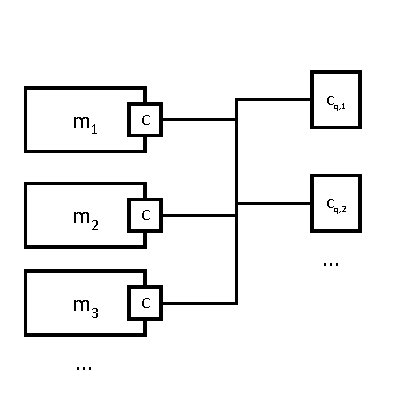
\includegraphics[width=2.3in,height=2.08125in]{fluidsystem}
\end{center}
\end{figure}

\begin{nonnormative}
The connection set represents an infinitesimally small control
volume, for which the stream connection equations are equivalent to the
conservation equations for mass and energy.
\end{nonnormative}

With these prerequisites, the semantics of the expression
\texttt{inStream(m\textsubscript i.c.h\_outflow)} is given implicitly by
defining an additional variable \texttt{h\_mix\_in\textsubscript{i}}, and by
adding to the model the conservation equations for mass and energy
corresponding to the infinitesimally small volume spanning the
connection set. The connection equation for the flow variables has
already been added to the system according to the connection semantics
of flow variables defined in \autoref{generation-of-connection-equations}.

\begin{lstlisting}[language=modelica,mathescape=true]
// Standard connection equation for flow variables
0 = sum(m_j.c.m_flow for j in 1:N) + sum(-ck.m_flow for k in 1:M);
\end{lstlisting}

Whenever the \lstinline!inStream()! operator is applied to a stream
variable of an inside connector, the balance equation of the transported
property must be added under the assumption of flow going into the
connector

\begin{lstlisting}[language=modelica]
// Implicit definition of the inStream() operator applied to inside connector i
0 = sum(mj.c.m_flow*(if mj.c.m_flow > 0 or j==i then h_mix_ini else mj.c.h_outflow)
        for j in 1:N) +
    sum(-ck.m_flow* (if -ck.m_flow > 0 then h_mix_ini else inStream(ck.h_outflow)
         for k in 1:M);
inStream(mi.c.h_outflow) = h_mix_ini;
\end{lstlisting}

Note that the result of the
\texttt{inStream(m\textsubscript{i}.c.h\_outflow)} operator is different
for each port \lstinline!i!, because the assumption of flow entering the port is
different for each of them.

Additional equations need to be generated for the stream variables of
outside connectors.

\begin{lstlisting}[language=modelica,mathescape=true]
// Additional connection equations for outside connectors
for q in 1:M loop
  0 = sum($m_j$.c.m_flow*(if
  $m_j$.c.m_flow > 0 then
  h_mix_out_q
  else $m_j$.c.h_outflow) for j
  in 1:N) +
  sum(-$c_k$.m_flow* (if
  -$c_k$.m_flow > 0 or k==q
  then h_mix_out$_q$
  else inStream($c_k$.h_outflow)
  for k in 1:M);
    $c_q$.h_outflow = h_mix_out$_q$;
  end for;
\end{lstlisting}

Neglecting zero flow conditions, the solution of the above-defined
stream connection equations for inStream values of inside connectors and
outflow stream variables of outside connectors is (for a derivation, see
\autoref{derivation-of-stream-equations}):

\begin{lstlisting}[language=modelica,mathescape=true]
inStream($m_i$.c.h_outflow) :=
  (sum(max(-$m_j$.c.m_flow,0)*$m_j$.c.h_outflow for j in cat(1,1:i-1, i+1:N) +
   sum(max( $c_k$.m_flow,0)*inStream($c_k$.h_outflow) for k in 1:M))/
  (sum(max(-$m_j$.c.m_flow,0) for j in  cat(1,1:i-1, i+1:N) +
   sum(max( $c_k$.m_flow ,0) for k in 1:M));

// Additional equations to be generated for outside connectors q
for q in 1:M loop
  $c_q$.h_outflow :=
    (sum(max(-$m_j$.c.m_flow,0)*$m_j$.c.h_outflow for j in 1:N) +
     sum(max( $c_k$.m_flow,0)*inStream($c_k$.h_outflow) for k in cat(1,1:q-1, q+1:M))/
    (sum(max(-$m_j$.c.m_flow,0) for j in  1:N) +
     sum(max( $c_k$.m_flow ,0) for k in cat(1,1:q-1, q+1:M)));
end for;
\end{lstlisting}

\emph{Note, that} \texttt{inStream(c\textsubscript{k}.h\_outflow)} \emph{is
computed from the connection set that is present one hierarchical level
above. At this higher level} \texttt{c\textsubscript{k}.h\_outflow} \emph{is no longer
an outside connector, but an inside connector and then the formula from
above for inside connectors can be used to compute it.}

If the argument of \lstinline!inStream()! is an array, the implicit
equation system holds elementwise, i.e., \lstinline!inStream()! is
vectorizable.

The stream connection equations have singularities and/or multiple
solutions if one or more of the flow variables become zero. When all the
flows are zero, a singularity is always present, so it is necessary to
approximate the solution in an open neighbourhood of that point.
{[}\emph{For example assume that} \texttt{m\textsubscript{j}.c.m\_flow =
c\textsubscript{k}.m\_flow = 0}\emph{, then all equations above are identically
fulfilled and \lstinline!inStream(..)! can have any value}{]}. However,
specific optimizations may be applied to avoid the regularization if the
flow through one port is zero or non-negative, see \autoref{derivation-of-stream-equations}. It is
required that the \lstinline!inStream()! operator is appropriately
approximated when regularization is needed and the approximation must
fulfill the following requirements:

\begin{enumerate}
\item
  \texttt{inStream(m\textsubscript{i}.c.h\_outflow)} and
  \texttt{inStream(c\textsubscript{k}.h\_outflow)} must be unique with
  respect to all values of the flow and stream variables in the
  connection set, and must have a continuous dependency on them.
\item
  Every solution of the implicit equation system above must fulfill the
  equation system identically {[}\emph{upto the usual numerical
  accuracy}{]}, provided the absolute value of every flow variable in
  the connection set is greater than a small value
  (\texttt{\textbar{}m\textsubscript{1}.c.m\_flow\textbar{} \textgreater{} eps
  \textbf{and} \textbar{}m\textsubscript{2}.c.m\_flow\textbar{}
  \textgreater{} eps \textbf{and} ... \textbf{and}
  \textbar{}c\textsubscript{M}.m\_flow\textbar{} \textgreater{} eps}).
\end{enumerate}

\begin{nonnormative}
Based on the above requirements, the following implementation is recommended:
\begin{itemize}
% This shouldn't be an itemized list, but a list of definitions
% faking that by using raggedright
\raggedright
\item \textbf{N = 1, M = 0:}\newline
\begin{lstlisting}[language=modelica,mathescape=true]
inStream($m_1$.c.h_outflow) =$m_1$.c.h_outflow;
\end{lstlisting}
\item
\textbf{N = 2, M = 0:}\newline
\begin{lstlisting}[language=modelica,mathescape=true]
inStream($m_1$.c.h_outflow) =$m_2$.c.h_outflow;
inStream($m_2$.c.h_outflow) =$m_1$.c.h_outflow;
\end{lstlisting}
\item \textbf{N = 1, M = 1:}\newline
\begin{lstlisting}[language=modelica,mathescape=true]
inStream($m_1$.c.h_outflow) =inStream($c_1$.h_outflow);
// Additional equation to be generated
$c_1$.h_outflow = $m_1$.c.h_outflow;
\end{lstlisting}
\item \textbf{N = 0, M = 2:}\newline
\begin{lstlisting}[language=modelica,mathescape=true]
// Additional equation to be generated
c1.h_outflow = inStream(c2.h_outflow);
c2.h_outflow = inStream(c1.h_outflow);
\end{lstlisting}

\item\textbf{All other cases:}\newline
\begin{lstlisting}[language=modelica,mathescape=true]
if $m_j$.c.m_flow.min >= 0  for all j = 1:N with j <> i  and
   $c_k$.m_flow.max <= 0 for all k = 1:M
then
    inStream($m_i$.c.h_outflow) =  $m_i$.c.h_outflow;
 else
    si = sum (max(-$m_j$.c.m_flow,0) for j in cat(1,1:i-1, i+1:N) +
         sum(max( $c_k$.m_flow ,0) for k  in 1:M);
    inStream($m_i$.c.h_outflow) =
       (sum(positiveMax(-$m_j$.c.m_flow,$s_i$)*$m_j$.c.h_outflow)
      +  sum(positiveMax($c_k$.m_flow,s_i)*inStream($c_k$.h_outflow)))/
     (sum(positiveMax(-$m_j$.c.m_flow,s_i))
        +  sum(positiveMax($c_k$.m_flow,s_i)))
                  for j in 1:N and i <> j and $m_j$.c.m_flow.min < 0,
                  for k in 1:M and $c_k$.m_flow.max > 0
// Additional equations to be generated
for q in 1:M loop
   if $m_j$.c.m_flow.min >= 0 for all j = 1:N and
       $c_k$.m_flow.max <= 0 for all k = 1:M and k <> q
   then
       $c_q$.h_outflow = 0;
    else
       $s_q$ =  (sum(max(-$m_j$.c.m_flow,0) for j in  1:N) +
                    sum(max( $c_k$.m_flow ,0) for k in cat(1,1:q-1, q+1:M)));
       $c_q$.h_outflow = (sum(positiveMax(-$m_j$.c.m_flow,s_q)*$m_j$.c.h_outflow) +
                 sum(positiveMax($c_k$.m_flow,$s_q$)* inStream($c_k$.h_outflow)))/
                (sum(positiveMax(-$m_j$.c.m_flow,s_q)) +
                 sum(positiveMax($c_k$.m_flow,s_q)))
		  for j in 1:N and $m_j$.c.m_flow.min < 0,
                  for k in 1:M and k <> q and $c_k$.m_flow.max > 0
end for;
\end{lstlisting}
\end{itemize}

The operator
\texttt{positiveMax(-m\textsubscript{j}.c.m\_flow,s\textsubscript{i})}
should be such that:
\begin{itemize}
\item
  positiveMax(-m\textsubscript{j}.c.m\_flow,s\textsubscript{i}) =
  -m\textsubscript{j}.c\_m\_flow if
  -m\textsubscript{j}.c.m\_flow\textgreater{}eps1\textsubscript{j}\textgreater{}=0,
  where eps1\textsubscript{j} are small flows, compared to typical
  problem-specific value,
\item
  all denominators should be \textgreater{} eps2 \textgreater{} 0,
  where eps2 is also a small flow, compared to typical problem-specific
  values.
\end{itemize}

Trivial implementation of positiveMax guarantees continuity of \lstinline!inStream()!:
\begin{lstlisting}[language=modelica,mathescape=true]
postiveMax(-$m_j$.c.m_flow, $s_i$)= max(-m_j.c.m_flow, eps1); // so $s_i$ is not needed
\end{lstlisting}
More sophisticated implementation, with smooth approximation, applied only when {all} flows are small:
\begin{lstlisting}[language=modelica,escapechar=!,mathescape=true]
// Define a "small number" eps (!\textbf{nominal}!(v) is the nominal value of v !--! see !\autoref{attributes-start-fixed-nominal-and-unbounded}!)
  eps := relativeTolerance*min(nominal($m_j$.c.m_flow));

// Define a smooth curve, such that  alpha($s_i>=eps$)=1 and alpha($s_i<0$)=0
  alpha := smooth(1, if $s_i$ > eps then 1 else
                     if $s_i$ > 0 then  ( $s_i$/eps)^2*(3-2* $s_i$/eps)) else 0);

  // Define function positiveMax(v,s_i) as a linear combination of max (v,0)
  // and of eps along alpha
  positiveMax((-$m_j$.c.m_flow,s_i)  := alpha*max(-$m_j$.c.m_flow,0) +  (1-alpha)*eps;
\end{lstlisting}

The derivation of this implementation is discussed in
\autoref{derivation-of-stream-equations}. Note that in the cases N = 1, M =0 (unconnected port,
physically corresponding to a plugged-up flange), and N = 2, M=0
(one-to-one connection), the result of \lstinline!inStream()! is trivial
and no non-linear equations are left in the model, despite the fact that
the original definition equations are nonlinear.

The following properties hold for this implementation:
\begin{itemize}
\item
  \lstinline!inStream(..)! is continuous (and differentiable),
  provided that \texttt{m\textsubscript{j}.c.h\_outflow,
  m\textsubscript{j}.c.m\_flow,
  c\textsubscript{k}.h\_outflow}, and
  \texttt{c\textsubscript{k}.m\_flow} are continuous and differentiable.
\end{itemize}

\begin{itemize}
\item
  A division by zero can no longer occur (since \texttt{sum(positiveMax(-m\textsubscript{j}.c.m\_flow,s\textsubscript{i}))\textgreater{}=eps2}
  \textgreater{} 0), so the result is always well-defined.
\item
  The balance equations are exactly fulfilled if the denominator
  is not close to zero\\
  (since the exact formula is used, if
  \texttt{sum(positiveMax(-m\textsubscript{j}.c.m\_flow,s\textsubscript{i})) \textgreater{} eps}).
\item
  If all flows are zero,
  \texttt{inStream(m\textsubscript{i}.c.h\_outflow) =
  sum(m\textsubscript{j}.c.h\_outflow for
  j\textless{}\textgreater{}i and m\textsubscript{j}.c.m\_flow.min \textless{}
  0)/Np}, i.e., it is the mean value of all the \lstinline!Np! variables
  \texttt{m\textsubscript{j}.c.h\_outflow}, such that \texttt{
  j\textless{}\textgreater{}i} and
  \texttt{m\textsubscript{j}.c.m\_flow.min \textless{} 0}. This is a
  meaningful approximation, considering the physical diffusion effects
  that are relevant at small flow rates in a small connection volume
  (thermal conduction for enthalpy, mass diffusion for mass fractions).
\end{itemize}

The value of relativeTolerance should be larger than the relative
tolerance of the nonlinear solver used to solve the implicit algebraic
equations.

As a final remark, further symbolic simplifications could be
carried out by taking into account equations that affect the flows in
the connection set (i.e., equivalent to m\textsubscript{j}.c.m\_flow =
0, which then implies m\textsubscript{j}.c.m\_flow.min \textgreater{}=
0). This is interesting, e.g., in the case of a valve when the stem
position is set identically to closed by its controller.
\end{nonnormative}

\section{Stream Operator actualStream}\doublelabel{stream-operator-actualstream}

The \lstinline!actualStream(v)! operator is provided for convenience, in
order to return the actual value of the stream variable, depending on
the actual flow direction. The only argument of this built-in operator
needs to be a reference to a stream variable. The operator is
vectorizable, in the case of vector arguments. For the following
definition it is assumed that an (inside or outside) connector \lstinline!c!
contains a stream variable \lstinline!h_outflow! which is associated with a flow
variable \lstinline!m_flow! in the same connector \lstinline!c!:

\begin{lstlisting}[language=modelica]
actualStream(c.h_outflow) = if c.m_flow > 0 then inStream(c.h_outflow) else c.h_outflow;
\end{lstlisting}

\begin{nonnormative}
The \textbf{actualStream}(v) operator is typically used in two
contexts:
\begin{lstlisting}[language=modelica]
  der(U) = c.m_flow*actualStream(c.h_outflow);  // (1)energy balance equation
  h_c = actualStream(c.h);                      // (2)monitoring the enthalpy at port c
\end{lstlisting}
In the case of equation (1), although the actualStream() operator
is discontinuous, the product with the flow variable is not, because
actualStream() is discontinuous when the flow is zero by construction.
Therefore, a tool might infer that the expression is smooth(0, ...)
automatically, and decide whether or not to generate an event. If a user
wants to avoid events entirely, he/she may enclose the right-hand side
of (1) with the noEvent() operator.

Equations like (2) might be used for monitoring purposes (e.g.
plots), in order to inspect what the actual enthalpy of the fluid
flowing through a port is. In this case, the user will probably want to
see the change due to flow reversal at the exact instant, so an event
should be generated. If the user doesn't bother, then he/she should
enclose the right-hand side of (2) with noEvent(). Since the output of
actualStream() will be discontinuous, it should not be used by itself to
model physical behaviour (e.g., to compute densities used in momentum
balances) - inStream() should be used for this purpose. The operator
actualStream() should be used to model physical behaviour only when
multiplied by the corresponding flow variable (like in the above energy
balance equation), because this removes the discontinuity.
\end{nonnormative}


% Synchronous Language Elements
\chapter{Synchronous Language Elements}\label{synchronous-language-elements}

This chapter defines synchronous behavior suited for implementation of control systems.
The synchronous behavior relies on an additional kind of discrete-time variables and equations, as well as an additional kind of \lstinline!when!-clause.
The benefits of synchronous behavior is that it allows a model to define large sampled data systems in a safe way, so that the translator can provide good a diagnostic in case of a modeling error.

The following small example shows the most important elements:
\begin{figure}[H]
  \begin{center}
    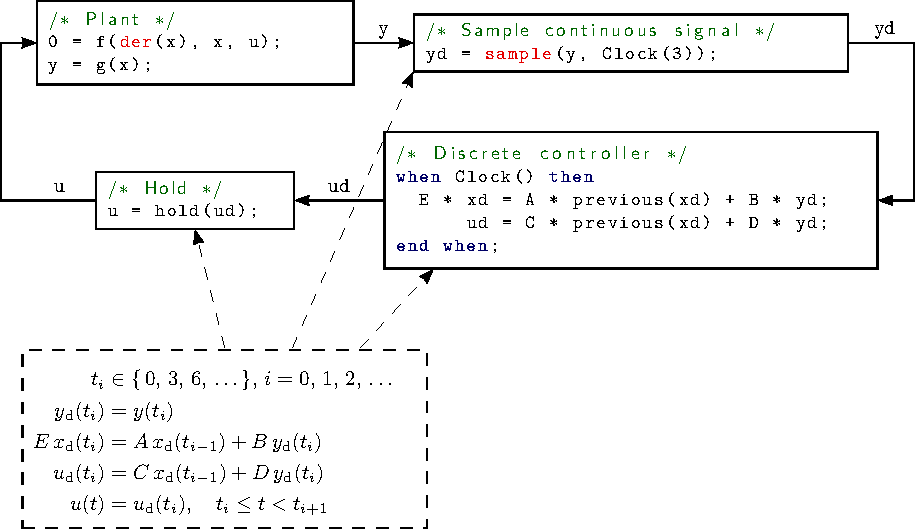
\includegraphics{plantmodel}
  \end{center}
  \caption{A continuous plant and a sampled data controller connected together with sample and (zero-order) hold elements.}
\end{figure}

\begin{itemize}
\item
  A periodic clock is defined with \lstinline!Clock(3)!.
  The argument of \lstinline!Clock! defines the sampling interval (for details see \cref{clock-constructors}).
\item
  Clocked variables (such as \lstinline!yd!, \lstinline!xd!, \lstinline!ud!) are associated uniquely with a clock and can only be directly accessed when the associated clock is active.
  Since all variables in a clocked equation must belong to the same clock, clocking errors can be detected at compile time.
  If variables from different clocks shall be used in an equation, explicit cast operators must be used, such as \lstinline!sample! to convert from continuous-time to clocked discrete-time or \lstinline!hold! to convert from clocked discrete-time to continuous-time.
\item
  A continuous-time variable is sampled at a clock tick with \lstinline!sample!.
  The operator returns the value of the continuous-time variable when the clock is active.
\item
  When no argument is defined for \lstinline!Clock!, the clock is deduced by clock inference.
\item
  For a \lstinline!when!-clause with an associated clock, all equations inside the \lstinline!when!-clause are clocked with the given clock.
  All equations on an associated clock are treated together and in the same way regardless of whether they are inside a \lstinline!when!-clause or not.
  This means that automatic sampling and hold of variables inside the \lstinline!when!-clause does not apply (explicit sampling and hold is required) and that general equations can be used in such \lstinline!when!-clauses (this is not allowed for \lstinline!when!-clauses with \lstinline!Boolean! conditions, that require a variable reference on the left-hand side of an equation).
\item
  The \lstinline!when!-clause in the controller could also be removed
  and the controller could just be defined by the equations:
\begin{lstlisting}[language=modelica]
/* Discrete controller */
E * xd = A * previous(xd) + B * yd;
    ud = C * previous(xd) + D * yd;
\end{lstlisting}
\item
  \lstinline!previous(xd)! returns the value of \lstinline!xd! at the previous clock tick.
  At the first sample instant, the start value of \lstinline!xd! is returned.
\item
  A discrete-time signal (such as \lstinline!ud!) is converted to a continuous-time signal with \lstinline!hold!.
\item
  If a variable belongs to a particular clock, then all other equations where this variable is used, with the exception of as argument to certain special operators, belong also to this clock, as well as all variables that are used in these equations.
  This property is used for clock inference and allows defining an associated clock only at a few places (above only in the sampler, whereas in the discrete controller and the hold the sampling period is inferred).
\item
  The approach in this chapter is based on the clock calculus and inference system proposed by \textcite{ColacoPouzet2003ClocksFirstClass} and implemented in Lucid Synchrone version 2 and 3 \parencite{Pouzet2006LucidSynchrone30}.
  However, the Modelica approach also uses multi-rate periodic clocks based on rational arithmetic introduced by \textcite{ForgetEtAl2008MultiPeriodic}, as an extension of the Lucid Synchrone semantics.
  These approaches belong to the class of synchronous languages \parencite{BenvenisteEtAl2003SynchronousTwelveYearsLater}.
\end{itemize}

\section{Rationale for Clocked Semantics}\label{rationale-for-clocked-semantics}

\begin{nonnormative}
Periodically sampled control systems could also be defined with standard \lstinline!when!-clauses, see \cref{when-equations}, and the \lstinline!sample! operator, see \cref{event-related-operators-with-function-syntax}.
For example:
\begin{lstlisting}[language=modelica]
when sample(0, 3) then
  xd = A * pre(xd) + B * y;
  u  = C * pre(xd) + D * y;
end when;
\end{lstlisting}

Equations in a \lstinline!when!-clause with a \lstinline!Boolean! condition have the
property that (a) variables on the left hand side of the equal sign are
assigned a value when the when-condition becomes true and otherwise hold
their value, (b) variables not assigned in the \lstinline!when!-clause are directly
accessed (= automatic \lstinline!sample! semantics), and (c) the variables
assigned in the \lstinline!when!-clause can be directly accessed outside of the
\lstinline!when!-clause (= automatic \lstinline!hold! semantics).

Using standard \lstinline!when!-clauses works well for individual simple sampled blocks, but the synchronous approach using clocks and clocked equations provide the following benefits (especially for large sampled systems):
\begin{enumerate}
\item
  Possibility to detect inconsistent sampling rate, since clock partitioning (see \cref{clock-partitioning}), replaces the automatic sample and hold semantics.
  Examples:
  \begin{enumerate}
  \def\labelenumii{\alph{enumii}.}
  \item
    If \lstinline!when!-clauses in different blocks should belong to the same
    controller part, but by accident different when-conditions are
    given, then this is accepted (no error is detected).
  \item
    If a sampled data library such as the Modelica\_LinearSystems2.Contoller library is used, at every block the sampling of the block has to be defined as integer multiple of a base sampling rate.
    If several blocks should belong to the same controller part, and different integer multiples are given, then the translator has to accept this (no error is detected).
  \end{enumerate}
  Note: Clocked systems can mix different sampling rates in well-defined ways when needed.
\item
  Fewer initial conditions are needed, as only a subset of clocked variables need initial conditions -- the clocked state variables (see \cref{clocked-state-variables}).
  For a standard \lstinline!when!-clause all variables assigned in a \lstinline!when!-clause must have an initial value because they might be used, before they are assigned a value the first time.
  As a result, all these variables are ``discrete-time states'' although in reality only a subset of them need an initial value.
\item
  More general equations can be used, compared to standard \lstinline!when!-clauses that require a restricted form of equations where the left hand side has to be a variable, in order to identify the variables that are assigned in the \lstinline!when!-clause.
  This restriction can be circumvented for standard \lstinline!when!-clauses, but is absent for clocked equations and make it more convenient to define nonlinear control algorithms.
\item
  Clocked equations allow clock inference, meaning that the sampling need only be given once for a sub-system.
  For a standard \lstinline!when!-clause the condition (sampling) must be explicitly propagated to all blocks, which is tedious and error prone for large systems.
\item
  Possible to use general continuous-time models in synchronous models (e.g., some advanced controllers use an inverse model of a plant in the feedforward path of the controller, see \textcite{ThummelEtAl2005InverseModels}).
  This powerful feature of Modelica to use a nonlinear plant model in a controller would require to export the continuous-time model with an embedded integration method and then import it in an environment where the rest of the controller is defined.
  With clocked equations, clocked controllers with continuous-time models can be directly defined in Modelica.
\item
  Clocked equations are straightforward to optimize because they are evaluated exactly once at each event instant.
  In contrast a standard \lstinline!when!-clause with \lstinline!sample! conceptually requires several evaluations of the model (in some cases tools can optimize this to avoid unneeded evaluations).
  The problem for the standard \lstinline!when!-clause is that after \lstinline!v! is changed, \lstinline!pre(v)! shall be updated and the model re-evaluated, since the equations could depend on \lstinline!pre(v)!.
  For clocked equations this iteration can be omitted since \lstinline!previous(v)! can only occur in the clocked equations that are only run the first event iterations.
\item
  Clocked subsystems using arithmetic blocks are straightforward to optimize.
  When a standard math-block (e.g., addition) is part of a clocked sub-system it is automatically clocked and only evaluated when the clocked equations trigger.
  For standard \lstinline!when!-clauses one either needs a separate sampled math-block for each operation, or it will conceptually be evaluated all the time.
  However, tools may perform a similar optimization for standard \lstinline!when!-clauses and it is only relevant in large sampled systems.
\end{enumerate}
\end{nonnormative}

\section{Definitions}\label{definitions}

In this section various terms are defined.

\subsection{Clocks and Clocked Variables}\label{clocks-and-clocked-variables}

% We can't use \subfloat just yet due to LaTeXML issue (fixed on master 2020-06-27):
%   https://github.com/brucemiller/LaTeXML/issues/1292 (marked as fixed as of commit 9f5c893b)
%\begin{figure}[tb]
%  \centering
%  \subfloat[A piecewise-constant variable.]{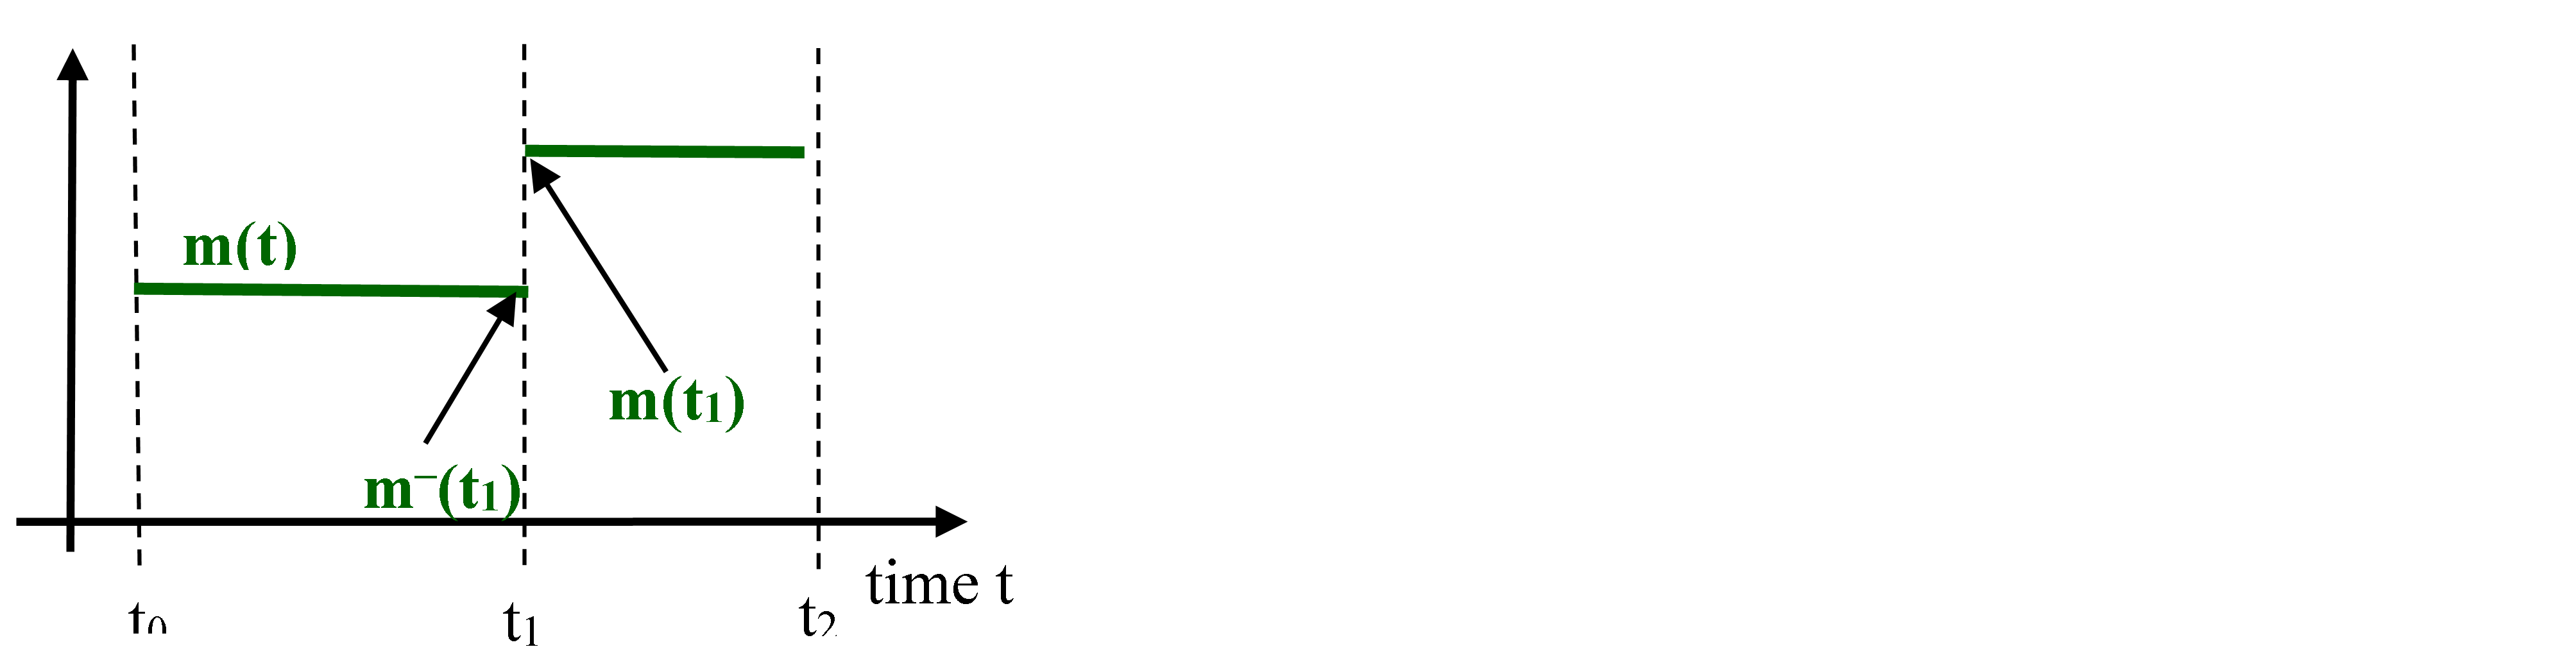
\includegraphics{piecewise}\label{fig:piecewise-constant-variable}}
%  \subfloat[A clock variable.]{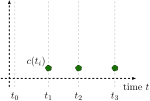
\includegraphics{clock}\label{fig:clock-variable}}
%  \subfloat[A clocked variable.]{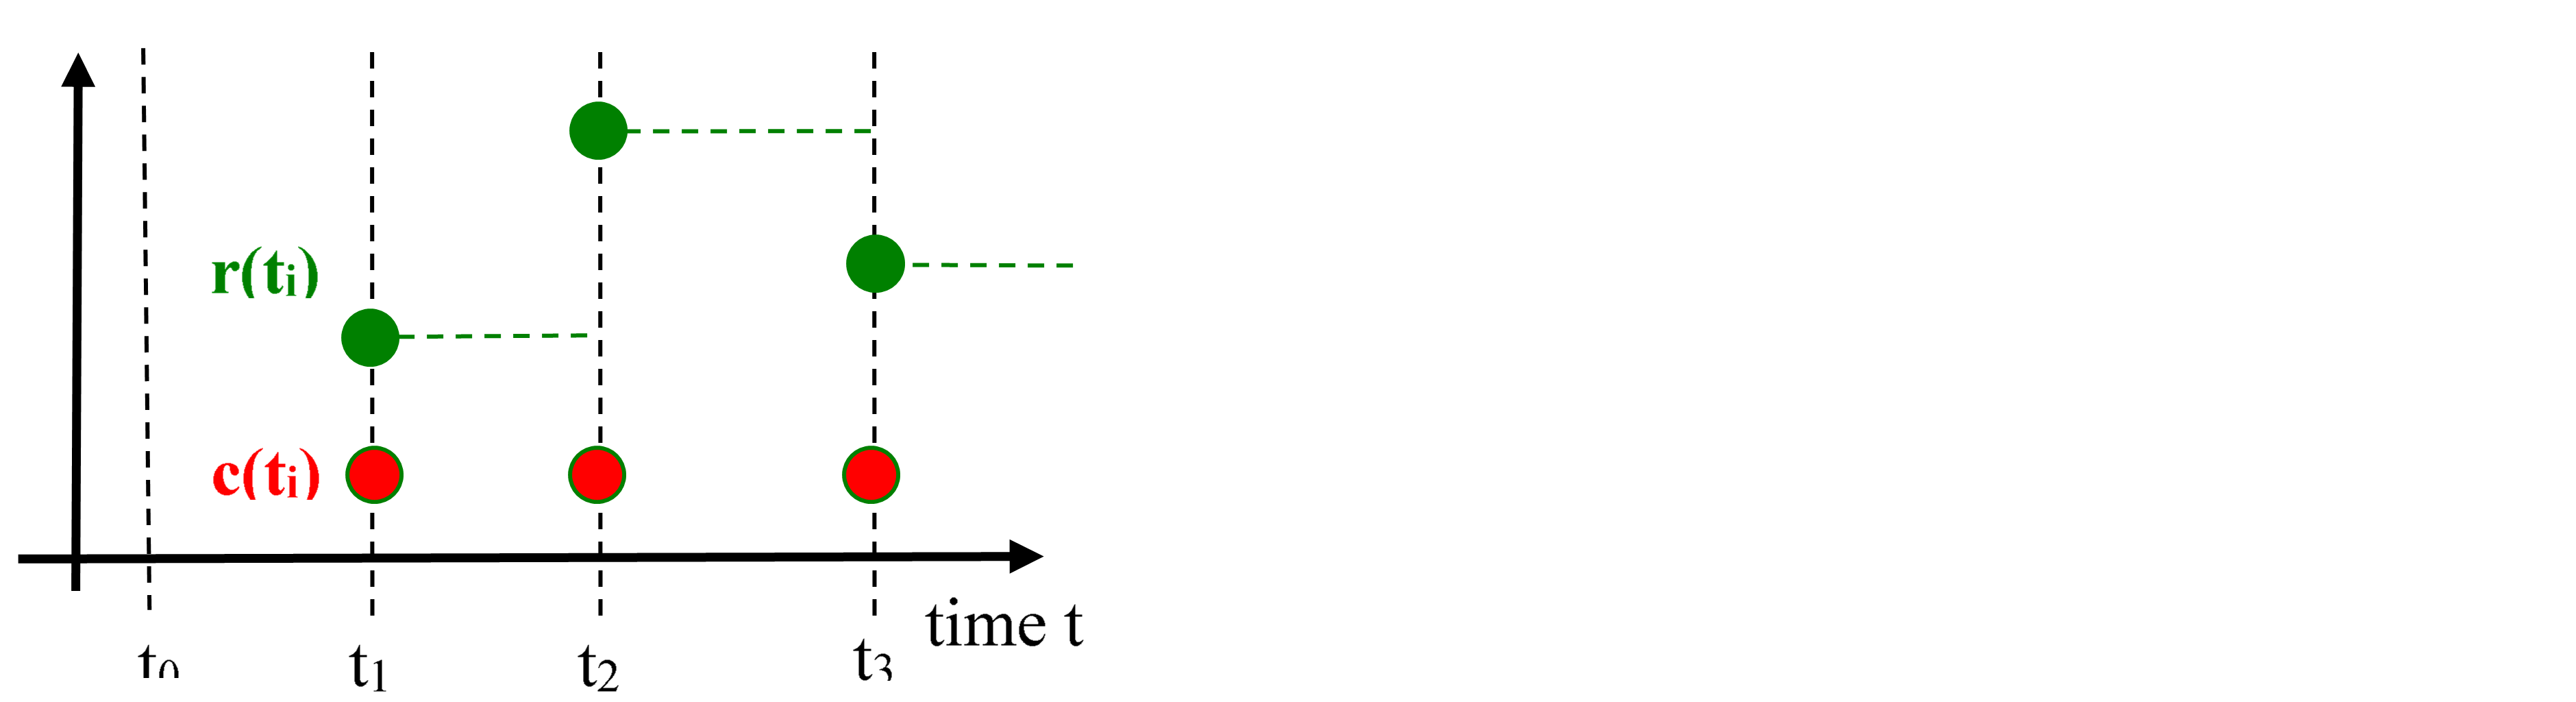
\includegraphics{clocked}\label{fig:clocked-variable}}
%  \caption{%
%    The different kinds of discrete-time variables.
%    The \lstinline!hold! extrapolation of the clocked variable is illustrated with dashed green lines.
%  }
%\end{figure}

In \cref{discrete-time-expressions} the term \emph{discrete-time} Modelica expression and in \cref{continuous-time-expressions} the term \emph{continuous-time} Modelica expression is defined.
In this chapter, two additional kinds of discrete-time expressions/variables are defined that are associated to clocks and are therefore called \firstuse[clocked!discrete-time expression]{clocked discrete-time}\index{expression variability!clocked discrete-time} expressions.
The different kinds of discrete-time variables in Modelica are defined below.

\begin{definition}[Piecewise-constant variable]\index{piecewise-constant variable}
(See \cref{discrete-time-expressions}.)
Variables $m(t)$ of base type \lstinline!Real!, \lstinline!Integer!, \lstinline!Boolean!, enumeration, and \lstinline!String! that are \emph{constant} inside each interval $t_{i} \leq t < t_{i+1}$ (i.e., piecewise constant continuous-time variables).
In other words, $m(t)$ changes value only at events: $m(t) = m(t_{i})$, for $t_{i} \leq t < t_{i+1}$.
Such variables depend continuously on time and they are discrete-time variables.
See \cref{fig:piecewise-constant-variable}.
\end{definition}

\begin{figure}[H]
  \begin{center}
    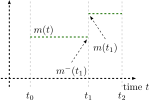
\includegraphics{piecewise-constant}
  \end{center}
  \caption{A piecewise-constant variable.}\label{fig:piecewise-constant-variable}
\end{figure}

\begin{definition}[Clock variable]\index{clock!variable}
Clock variables $c(t_{i})$ are of base type \lstinline!Clock!\indexinline{Clock}.
A clock is either defined by a constructor (such as \lstinline!Clock(3)!) that defines when the clock ticks (is active) at a particular time instant, or it is defined with clock operators relatively to other clocks, see \cref{base-clock-conversion-operators}.
See \cref{fig:clock-variable}.
\end{definition}

\begin{example}
Clock variables:
\begin{lstlisting}[language=modelica]
Clock c1 = Clock($\ldots$);
Clock c2 = c1;
Clock c3 = subSample(c2, 4);
\end{lstlisting}
\end{example}

\begin{figure}[H]
  \begin{center}
    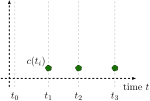
\includegraphics{clock}
  \end{center}
  \caption{%
    A clock variable.
    The value of a clock variable is not defined -- the plot marks only indicate \emph{when} the clock is active.
  }\label{fig:clock-variable}
\end{figure}

\begin{definition}[Clocked variable]\label{def:clocked-variable}\index{clocked!variable}
The elements of clocked variables $r(t_{i})$ are of base type \lstinline!Real!, \lstinline!Integer!, \lstinline!Boolean!, enumeration, \lstinline!String! that are associated uniquely with a clock $c(t_{i})$.
A clocked variable can only be directly accessed at the event instant where the associated clock is active.
A constant and a parameter can always be used at a place where a clocked variable is required.
\begin{nonnormative}
Note that clock variables are not included in this list.
This implies that clock variables cannot be used where clocked variables are required.
\end{nonnormative}

At time instants where the associated clock is not active, the value of a clocked variable can be inquired by using an explicit cast operator, see below.
In such a case \lstinline!hold! semantics is used, in other words the value of the clocked variable from the last event instant is used.
See \cref{fig:clocked-variable}.
\end{definition}

\begin{figure}[H]
  \begin{center}
    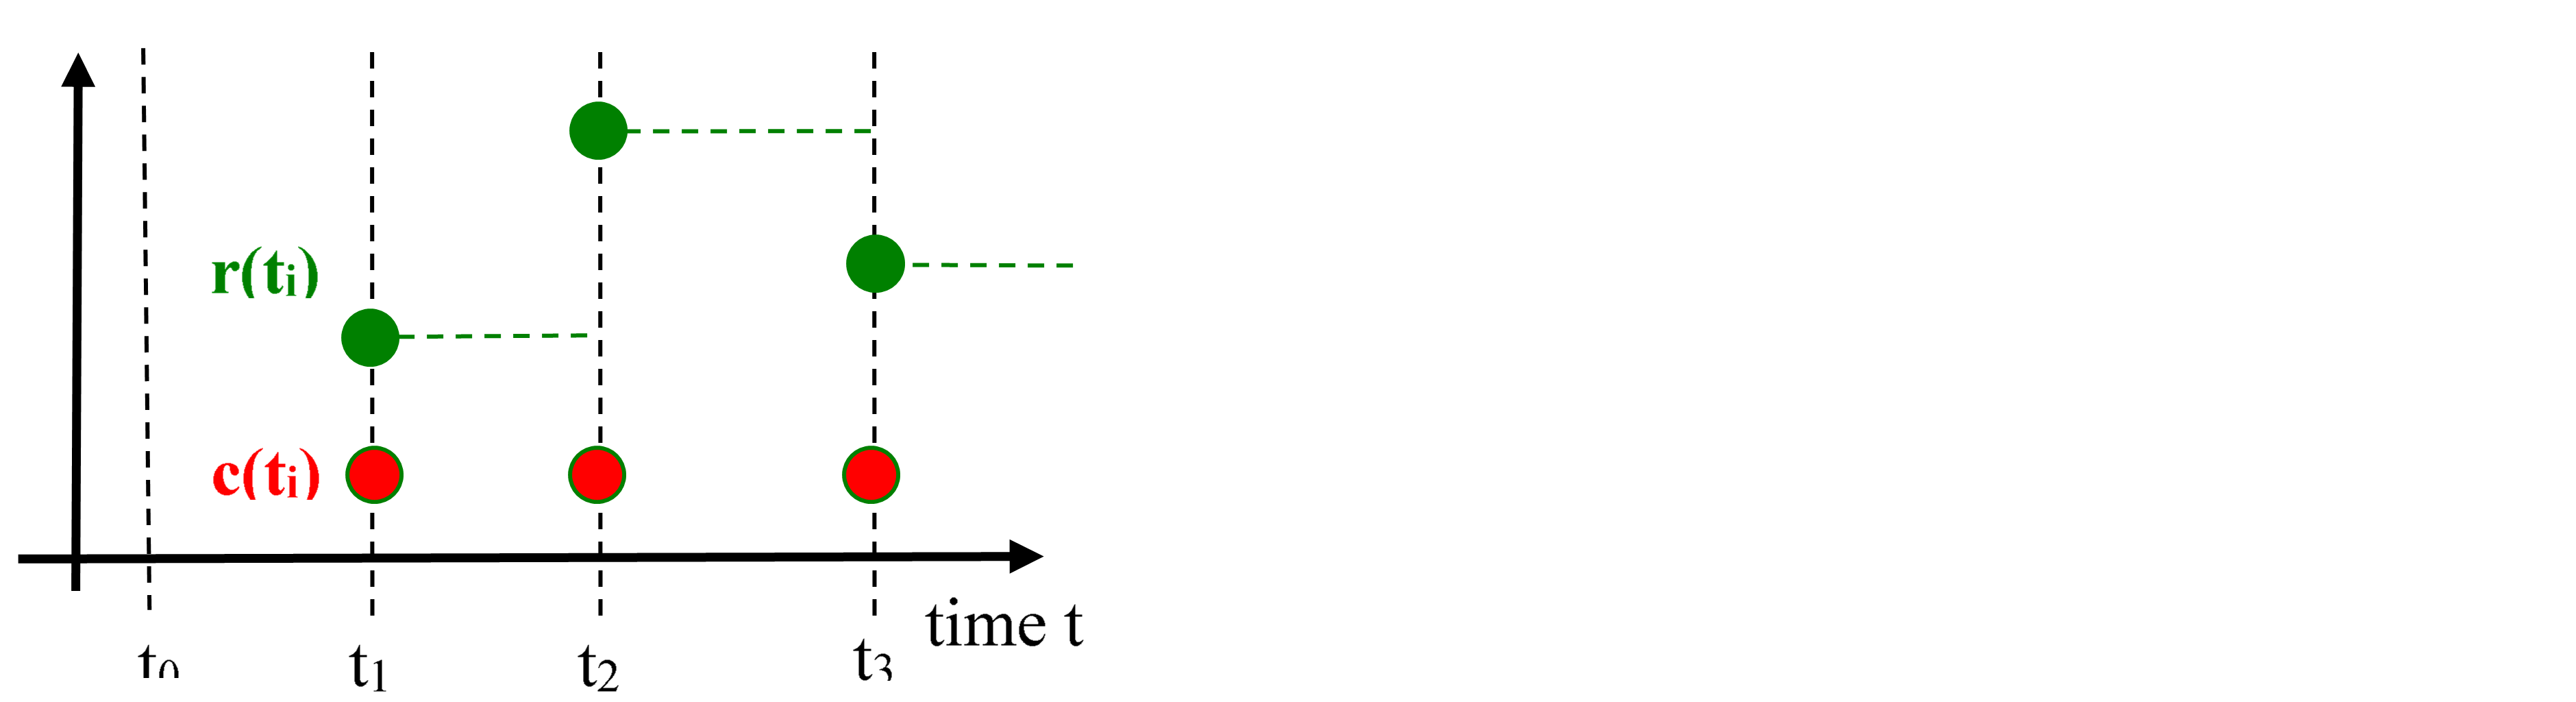
\includegraphics{clocked}
  \end{center}
  \caption{
    A clocked variable.
    The \lstinline!hold! extrapolation of the value at the last event instant is illustrated with dashed green lines.
  }\label{fig:clocked-variable}
\end{figure}

\subsection{Base-Clock and Sub-Clock Partitions}\label{base-clock-and-sub-clock-partitions}

There are two kinds of \firstuse[clock!partition]{clock partitions}:

\begin{definition}[Base-clock partition]\index{base-clock partition}\index{clock!partition!base-clock}
A base-clock partition identifies a set of equations and a set of variables which must be executed together in one task.
Different base-clock partitions can be associated to separate tasks for asynchronous execution.
\end{definition}

\begin{definition}[Sub-clock partition]\index{sub-clock partition}\index{clock!partition!sub-clock}
A sub-clock partition identifies a subset of equations and a subset of variables of a base-clock partition which are partially synchronized with other sub-clock partitions of the same base-clock
partition, i.e., synchronized when the ticks of the respective clocks are simultaneous.
\end{definition}

\subsection{Argument Restrictions (Component Expression)}\label{argument-restrictions-component-expression}

The built-in operators (with function syntax) defined in the following sections have partially restrictions on their input arguments that are not present for Modelica functions.
To define the restrictions, the following term is used.

\begin{definition}[Component expression]\label{def:component-expression}\index{component!expression (argument restriction)}
A component expression is a \lstinline[language=grammar]!component-reference! which is a valid expression, i.e., not referring to models or blocks with equations.
% "an element of records" below looks strange:
In detail, it is an instance of a (a) base type, (b) derived type, (c) record, (d) an array of such an instance (a-c), (e) one or more elements of such an array (d) defined by index expressions which are parameter expressions (see below), or (f) an element of records.
\begin{nonnormative}
The essential features are that one or several values are associated with the instance, that start values can be defined on these values, and that no equations are associated with the instance.
A component expression can be constant or can vary with time.
\end{nonnormative}
\end{definition}

In the following sections, when defining an operator with function calling syntax, there are some common restrictions being used for the input arguments (operands).
For example, an input argument to the operator may be required to be a component expression (\cref{def:component-expression}) or parameter expression (\cref{variability-of-expressions}).
To emphasize that there are no such restrictions, an input argument may be said to be just an \emph{expression}.

\begin{nonnormative}
The reason for restricting an input argument to be a component expression is that the start value of the input argument is returned before the first tick of the clock of the input argument and this
is not possible for a general expression.

The reason for restricting an input argument to be a parameter expression is that the value of the input argument needs to be evaluated during translation, in order that clock analysis can be performed during translation.
\end{nonnormative}

\begin{example}
The input argument to \lstinline!previous! is restricted to be a component expression.
\begin{lstlisting}[language=modelica]
Real u1;
Real u2[4];
Complex c;
Resistor R;
$\ldots$
y1 = previous(u1);    // fine
y2 = previous(u2);    // fine
y3 = previous(u2[2]); // fine
y4 = previous(c.im);  // fine
y5 = previous(2 * u); // error (general expression, not component expression)
y6 = previous(R);     // error (component, not component expression)
\end{lstlisting}
\end{example}

\begin{example}
The named argument \lstinline!factor! of \lstinline!subSample! is restricted to be a parameter expression.
\begin{lstlisting}[language=modelica]
Real u;
parameter Real p=3;
$\ldots$
y1 = subSample(u, factor = 3);         // fine (literal)
y2 = subSample(u, factor = 2 * p - 3); // fine (parameter expression)
y3 = subSample(u, factor = 3 * u);     // error (general expression)
\end{lstlisting}
\end{example}

None of the operators defined in this chapter vectorize, but some can operate directly on array variables (including clocked array variables, but not clock array variables).
They are not callable in functions.

\section{Clock Constructors}\label{clock-constructors}

The overloaded constructors listed below are available to generate clocks, and it is possible to call them with the specified named arguments, or with positional arguments (according to the order shown in the details after the table).
\begin{center}
\begin{tabular}{l|l l}
\hline
\tablehead{Expression} & \tablehead{Description} & \tablehead{Details}\\
\hline
\hline
{\lstinline!Clock()!} & Inferred clock & \Cref{modelica:clock-inferred}\\
{\lstinline!Clock(intervalCounter, resolution)!} & Rational interval clock & \Cref{modelica:clock-rational}\\
{\lstinline!Clock(interval)!} & Real interval clock & \Cref{modelica:clock-interval}\\
{\lstinline!Clock(condition, startInterval)!} & Event clock & \Cref{modelica:clock-event}\\
{\lstinline!Clock(c, solverMethod)!} & Solver clock & \Cref{modelica:clock-solver}\\
\hline
\end{tabular}
\end{center}

\begin{operatordefinition*}[Clock]\label{modelica:clock-inferred}\index{Clock@\robustinline{Clock}!inferred}
\begin{synopsis}\begin{lstlisting}
Clock()
\end{lstlisting}\end{synopsis}
\begin{semantics}
\firstuse[inferred clock]{Inferred clock}.
The operator returns a clock that is inferred.

\begin{example}
\begin{lstlisting}[language=modelica]
when Clock() then // equations are on the same clock
  x = A * previous(x) + B * u;
  Modelica.Utilities.Streams.print
    ("clock ticks at = " + String(sample(time)));
end when;
\end{lstlisting}
Note, in most cases, the operator is not needed and equations could be written without a \lstinline!when!-clause (but not in the example above, since the \lstinline!print! statement is otherwise not associated to a clock).
This style is useful if a modeler would clearly like to mark the equations that must belong to one clock (although a tool could figure this out as well, if the \lstinline!when!-clause is not present).
\end{example}
\end{semantics}
\end{operatordefinition*}

\begin{operatordefinition*}[Clock]\label{modelica:clock-rational}\index{Clock@\robustinline{Clock}!rational}
\begin{synopsis}\begin{lstlisting}
Clock(intervalCounter=$\mathit{intervalCounter}$, resolution=$\mathit{resolution}$)
\end{lstlisting}\end{synopsis}
\begin{semantics}
\firstuse[rational interval clock]{Rational interval clock}.
The first input argument, $\mathit{intervalCounter}$, is a clocked component expression (\cref{def:component-expression}) or a parameter expression of type \lstinline!Integer! with \lstinline!min = 0!.
The optional second argument $\mathit{resolution}$ (defaults to 1) is a parameter expression of type \lstinline!Integer! with \lstinline!min = 1! and \lstinline!unit = "Hz"!.
If $\mathit{intervalCounter}$ is a parameter expression with value zero, the period of the clock is derived by clock inference, see \cref{sub-clock-inferencing}.

If $\mathit{intervalCounter}$ is a parameter expression greater than zero, the clock defines a periodic clock.
If $\mathit{intervalCounter}$ is a clocked component expression it must be greater than zero.
The result is of base type \lstinline!Clock! that ticks when \lstinline!time! becomes $t_{\mathrm{start}}$, $t_{\mathrm{start}} + \mathit{interval}_{1}$, $t_{\mathrm{start}} + \mathit{interval}_{1} + \mathit{interval}_{2}$, \@\ldots{}
The clock starts at the start of the simulation $t_{\mathrm{start}}$ or when the controller is switched on.
At the start of the simulation, \lstinline!previous($\mathit{intervalCounter}$)! = \lstinline!$\mathit{intervalCounter}$.start! and the clocks ticks the first time.
At the first clock tick $\mathit{intervalCounter}$ must be computed and the second clock tick is then triggered at $\mathit{interval}_{1} = \mathit{intervalCounter}/\mathit{resolution}$.
At the second clock tick at time $t_{\mathrm{start}} + \mathit{interval}_{1}$, a new value for $\mathit{intervalCounter}$ must be computed and the next clock tick is scheduled at $\mathit{interval}_{2} = \mathit{intervalCounter}/\mathit{resolution}$, and so on.


\begin{nonnormative}
The given interval and time shift % What given "interval" and "time shift"?
can be modified by using the \lstinline!subSample!, \lstinline!superSample!, \lstinline!shiftSample! and \lstinline!backSample! operators on the returned clock, see \cref{sub-clock-conversion-operators}.
\end{nonnormative}

\begin{example}
\begin{lstlisting}[language=modelica]
  // first clock tick: previous(nextInterval) = 2
  Integer nextInterval(start = 2);
  Real y1(start = 0);
  Real y2(start = 0);
equation
  when Clock(2, 1000) then
    // periodic clock that ticks at 0, 0.002, 0.004, $\ldots$
    y1 = previous(y1) + 1;
  end when;

  when Clock(nextInterval, 1000) then
    // interval clock that ticks at 0, 0.003, 0.007, 0.012, $\ldots$
    nextInterval = previous(nextInterval) + 1;
    y2 = previous(y2) + 1;
  end when;
\end{lstlisting}
\end{example}

Note that operator \lstinline!interval(c)! of \lstinline!Clock c = Clock(nextInterval, $\mathit{resolution}$)! returns:\newline
\lstinline!previous($\mathit{intervalCounter}$) / $\mathit{resolution}$! (in seconds)
\end{semantics}
\end{operatordefinition*}

\begin{operatordefinition*}[Clock]\label{modelica:clock-interval}\index{Clock@\robustinline{Clock}!interval}
\begin{synopsis}\begin{lstlisting}
Clock(interval=$\mathit{interval}$)
\end{lstlisting}\end{synopsis}
\begin{semantics}
\firstuse[real interval clock]{Real interval clock}.
The input argument, $\mathit{interval}$, is a clocked component expression (\cref{def:component-expression}) or a parameter expression.
The $\mathit{interval}$ must be strictly positive ($\mathit{interval} > 0$) of type \lstinline!Real! with \lstinline!unit = "s"!.
The result is of base type \lstinline!Clock! that ticks when \lstinline!time! becomes $t_{\mathrm{start}}$, $t_{\mathrm{start}} + \mathit{interval}_{1}$, $t_{\mathit{start}} + \mathit{interval}_{1} + \mathit{interval}_{2}$, \@\ldots{}
The clock starts at the start of the simulation $t_{\mathrm{start}}$ or when the controller is switched on.
Here the next clock tick is scheduled at $\mathit{interval}_{1}$ = \lstinline!previous($\mathit{interval}$)! = \lstinline!$\mathit{interval}$.start!.
At the second clock tick at time $t_{\mathrm{start}} + \mathit{interval}_{1}$, the next clock tick is scheduled at $\mathit{interval}_{2}$ = \lstinline!previous($\mathit{interval}$)!, and so on.
If $\mathit{interval}$ is a parameter expression, the clock defines a periodic clock.

\begin{nonnormative}
Note, the clock is defined with \lstinline!previous($\mathit{interval}$)!.
Therefore, for sorting the input argument is treated as known.
The given interval and time shift can be modified by using the \lstinline!subSample!, \lstinline!superSample!, \lstinline!shiftSample! and \lstinline!backSample! operators on the returned clock, see \cref{sub-clock-conversion-operators}.
There are restrictions where this operator can be used, see \lstinline!Clock! expressions below.
\end{nonnormative}
\end{semantics}
\end{operatordefinition*}

\begin{operatordefinition*}[Clock]\label{modelica:clock-event}\index{Clock@\robustinline{Clock}!event}
\begin{synopsis}\begin{lstlisting}
Clock(condition=$\mathit{condition}$, startInterval=$\mathit{startInterval}$)
\end{lstlisting}\end{synopsis}
\begin{semantics}
\firstuse[event clock]{Event clock}.
The first input argument, $\mathit{condition}$, is a continuous-time expression of type \lstinline!Boolean!.
The optional $\mathit{startInterval}$ argument (defaults to 0) is the value returned by \lstinline!interval()! at the first tick of the clock, see \cref{initialization-of-clocked-partitions}.
The result is of base type \lstinline!Clock! that ticks when \lstinline!edge($\mathit{condition}$)! becomes \lstinline!true!.
\begin{nonnormative}
This clock is used to trigger a clocked partition due to a state event, that is a zero-crossing of a \lstinline!Real! variable, in a continuous-time partition or due to a hardware interrupt that is modeled as \lstinline!Boolean! in the simulation model.
\end{nonnormative}

\begin{example}
\begin{lstlisting}[language=modelica]
Clock c = Clock(angle > 0, 0.1); // before first tick of c:
                                 // interval(c) = 0.1
\end{lstlisting}
\end{example}

\begin{nonnormative}
The implicitly given interval and time shift can be modified by using the \lstinline!subSample!, \lstinline!superSample!, \lstinline!shiftSample! and \lstinline!backSample! operators on the returned clock, see \cref{sub-clock-conversion-operators}, provided the base interval is not smaller than the implicitly given interval.
\end{nonnormative}
\end{semantics}
\end{operatordefinition*}

\begin{operatordefinition*}[Clock]\label{modelica:clock-solver}\index{Clock@\robustinline{Clock}!solver}
\begin{synopsis}\begin{lstlisting}
Clock(c=$c$, solverMethod=$\mathit{solverMethod}$)
\end{lstlisting}\end{synopsis}
\begin{semantics}
\firstuse[solver clock]{Solver clock}.
The first input argument, $c$, is a clock and the operator returns this clock.
The returned clock is associated with the second input argument $\mathit{solverMethod}$ of type \lstinline!String!.
The meaning of $\mathit{solverMethod}$ is defined in \cref{solver-methods}.
If $\mathit{solverMethod}$ is the empty \lstinline!String!, then this \lstinline!Clock! construct does not associate an integrator with the returned clock.

\begin{example}
\begin{lstlisting}[language=modelica]
Clock c1 = Clock(1, 10);                   // 100 ms, no solver
Clock c2 = Clock(c1, "ImplicitTrapezoid"); // 100 ms, ImplicitTrapezoid solver
Clock c3 = Clock(c2, "");                  // 100 ms, no solver
\end{lstlisting}
\end{example}
\end{semantics}
\end{operatordefinition*}

Besides inferred clocks and solver clocks, one of the following mutually
exclusive associations of clocks are possible in one base partition:
\begin{enumerate}
\item
  One or more rational interval clocks, provided they are consistent with each other, see \cref{sub-clock-inferencing}.
  \begin{example}
  Assume \lstinline!y = subSample(u)!, and \lstinline!Clock(1, 10)! is associated with \lstinline!u! and \lstinline!Clock(2, 10)! is associated with \lstinline!y!, then this is correct, but it would be an error if \lstinline!y! is associated with a \lstinline!Clock(1, 3)!.
  \end{example}
\item
  Exactly one real interval clock.
  \begin{example}
  Assume \lstinline!Clock c = Clock(2.5)!, then variables in the same base partition can be associated multiple times with \lstinline!c! but not multiple times with \lstinline!Clock(2.5)!.
  \end{example}
\item
  Exactly one event clock.
\item
  A default clock, if neither a real interval, nor a rational interval nor an event clock is associated with a base partition.
  In this case the default clock is associated with the fastest sub-clock partition.
  \begin{nonnormative}
  Typically, a tool will use \lstinline!Clock(1.0)! as a default clock and will raise a warning, that it selected a default clock.
  \end{nonnormative}
\end{enumerate}

Clock variables can be used in a restricted form of expressions.
Generally, every expression switching between clock variables must have parameter variability (in order that clock analysis can be performed when translating a model).
Thus subscripts on clock variables and conditions of if-then-else switching between clock variables must be parameter expressions, and there are similar restrictions for sub-clock conversion operators \cref{sub-clock-conversion-operators}.
Otherwise, the following expressions are allowed:
\begin{itemize}
\item
  Declaring arrays of clocks.
  \begin{example}
  \lstinline!Clock c1[3] = {Clock(1), Clock(2), Clock(3)}!
  \end{example}
% Ok, that bug in pdflatex was weird: \emph{Example: \lstinline!Clock c1[3] ={Clock(1), Clock(2), Clock(3)}!} {]}
\item
  Array constructors of clocks: \lstinline!{}!, \lstinline![]!, \lstinline!cat!.
\item
  Array access of clocks.
  \begin{example}
  \lstinline!sample(u, c1[2])!
  \end{example}
\item
  Equality of clocks.
  \begin{example}
  \lstinline!c1 = c2!
  \end{example}
\item
  \lstinline!if!-expressions of clocks in equations.
  \begin{example}
\begin{lstlisting}[language=modelica]
Clock c2 =
  if f > 0 then
    subSample(c1, f)
  elseif f < 0 then
    superSample(c1, f)
  else
    c1;
\end{lstlisting}
  \lstinline!!
  \end{example}
\item
  Clock variables can be declared in models, blocks, connectors, and records.
  A clock variable can be declared with the prefixes \lstinline!input!, \lstinline!output!, \lstinline!inner!, \lstinline!outer!, but \emph{not} with the prefixes \lstinline!flow!, \lstinline!stream!, \lstinline!discrete!, \lstinline!parameter!, or \lstinline!constant!.
  \begin{example}
\begin{lstlisting}[language=modelica]
connector ClockInput = input Clock;
\end{lstlisting}
  \end{example}
\end{itemize}

\section{Clocked State Variables}\label{clocked-state-variables}

\begin{definition}[Clocked state variable]\label{def:clocked-state-variable}\index{clocked!state variable}\index{state variable!clocked}
A component expression which is not a parameter, and to which \lstinline!previous! has been applied.
\end{definition}

The previous value of a clocked variable can be accessed with the \lstinline!previous! operator, listed below.
\begin{center}
\begin{tabular}{l|l l}
\hline
\tablehead{Expression} & \tablehead{Description} & \tablehead{Details}\\
\hline
\hline
{\lstinline!previous($u$)!} & Previous value of clocked variable & \Cref{modelica:previous} \\
\hline
\end{tabular}
\end{center}

\begin{operatordefinition}[previous]
\begin{synopsis}\begin{lstlisting}
previous($u$)
\end{lstlisting}\end{synopsis}
\begin{semantics}
The input argument $u$ is a component expression (\cref{def:component-expression}).
If $u$ is a parameter, its value is returned.

Otherwise:
Input and return arguments are on the same clock.
At the first tick of the clock of $u$ or after a reset transition (see \cref{reset-handling}), the start value of $u$ is returned, see \cref{initialization-of-clocked-partitions}.
At subsequent activations of the clock of $u$, the value of $u$ from the previous clock activation is returned.
\end{semantics}
\end{operatordefinition}

\begin{nonnormative}
At a clock tick only the (previous) values of the clocked state variables are needed to compute the new values of all clocked variables on that clock.
This roughly corresponds to state variables in continuous time.
\end{nonnormative}

\section{Partitioning Operators}\label{partitioning-operators}

A set of \emph{clock conversion operators} together act as boundaries
between different clock partitions.

\subsection{Base-Clock Conversion Operators}\label{base-clock-conversion-operators}

The operators listed below convert between a continuous-time and a clocked-time representation and vice versa.
\begin{center}
\begin{tabular}{l|l l}
\hline
\tablehead{Expression} & \tablehead{Description} & \tablehead{Details}\\
\hline
\hline
{\lstinline!sample($u$, $\mathit{clock}$)!} & Sample continuous-time expression & \Cref{modelica:clocked-sample} \\
{\lstinline!hold($u$)!} & Zeroth order hold of clocked-time variable & \Cref{modelica:hold} \\
\hline
\end{tabular}
\end{center}

\begin{operatordefinition*}[sample]\label{modelica:clocked-sample}\index{sample@\robustinline{sample}!clocked}
\begin{synopsis}\begin{lstlisting}
sample($u$, $\mathit{clock}$)
\end{lstlisting}\end{synopsis}
\begin{semantics}
Input argument $u$ is a continuous-time expression according to \cref{continuous-time-expressions}.
The optional input argument $\mathit{clock}$ is of type \lstinline!Clock!, and can in a call be given as a named argument (with the name $\mathit{clock}$), or as positional argument.
The operator returns a clocked variable that has $\mathit{clock}$ as associated clock and has the value of the left limit of $u$ when $\mathit{clock}$ is active (that is the value of $u$ just before the event of $\mathit{clock}$ is triggered).
If $\mathit{clock}$ is not provided, it is inferred, see \cref{sub-clock-inferencing}.
\begin{nonnormative}
Since the operator returns the left limit of $u$, it introduces an infinitesimal small delay between the continuous-time and the clocked partition.
This corresponds to the reality, where a sampled data system cannot act infinitely fast and even for a very idealized simulation, an infinitesimal small delay is present.
The consequences for the sorting are discussed below.

Input argument $u$ can be a general expression, because the argument is continuous-time and therefore has always a value.
It can also be a constant, a parameter or a piecewise constant expression.

Note that \lstinline!sample! is an overloaded function:
If \lstinline!sample! has two positional input arguments and the second argument is of type \lstinline!Real!, it is the operator from \cref{event-related-operators-with-function-syntax}.
If \lstinline!sample! has one input argument, or it has two input arguments and the second argument is of type \lstinline!Clock!, it is the base-clock conversion operator from this section.
\end{nonnormative}
\end{semantics}
\end{operatordefinition*}

\begin{operatordefinition}[hold]
\begin{synopsis}\begin{lstlisting}
hold($u$)
\end{lstlisting}\end{synopsis}
\begin{semantics}
Input argument $u$ is a clocked (\cref{def:clocked-variable}) component expression (\cref{def:component-expression}) or a parameter expression.
The operator returns a piecewise constant signal of the same type as $u$.
When the clock of $u$ ticks, the operator returns $u$ and otherwise returns the value of $u$ from the last clock activation.
Before the first clock activation of $u$, the operator returns the start value of $u$, see \cref{initialization-of-clocked-partitions}.
\begin{nonnormative}
Since the input argument is not defined before the first tick of the clock of $u$, the restriction is present, that it must be a component expression (or a parameter expression), in order that the initial value of $u$ can be used in such a case.
\end{nonnormative}
\end{semantics}
\end{operatordefinition}

\begin{example}
Assume there is the following model:
\begin{lstlisting}[language=modelica]
  Real y(start = 1), yc;
equation
  der(y) + y = 2;
  yc = sample(y, Clock(0.1));
initial equation
  der(y) = 0;
\end{lstlisting}

The value of \lstinline!yc! at the first clock tick is $\text{\lstinline!yc!} = 2$ (and not $\text{\lstinline!yc!} = 1$).
The reason is that the continuous-time model \lstinline!der(y) + y = 2! is first initialized and after initialization \lstinline!y! has the value 2.
At the first clock tick at $\text{\lstinline!time!} = 0$, the left limit of \lstinline!y! is 2 and therefore $\text{\lstinline!yc!} = 2$.
\end{example}

\subsubsection{Sorting of a Simulation Model}

\begin{nonnormative}
Since \lstinline!sample(u)! returns the left limit of \lstinline!u!, and the left limit of \lstinline!u! is a known value, all inputs to a base-clock partition are treated as known during sorting.
Since a periodic and interval clock can tick at most once at a time instant, and since the left limit of a variable does not change during event iteration (i.e., re-evaluating a base-clock partition associated with a condition clock always gives the same result because the \lstinline!sample(u)! inputs do not change and therefore need not to be re-evaluated) all base-clock partitions, see \cref{base-clock-partitioning}, need not to be sorted with respect to each other.
Instead, at an event instant, active base-clock partitions can be evaluated first (and once) in any order.
Afterwards, the continuous-time partition is evaluated.

Event iteration takes place only over the continuous-time partition.
In such a scenario, accessing the left limit of \lstinline!u! in \lstinline!sample(u)! just means to pick the latest available value of \lstinline!u! when the partition is entered, storing it in a local variable of the partition and only using this local copy during evaluation of the equations in this partition.
\end{nonnormative}

\subsection{Sub-Clock Conversion Operators}\label{sub-clock-conversion-operators}

The operators listed below convert between synchronous clocks.
\begin{center}
\begin{tabular}{l|l l}
\hline
\tablehead{Expression} & \tablehead{Description} & \tablehead{Details}\\
\hline
\hline
{\lstinline!subSample($u$, factor)!} & Clock that is slower by a factor  & \Cref{modelica:subSample}\\
{\lstinline!superSample($u$, factor)!} & Clock that is faster by a factor  & \Cref{modelica:superSample}\\
{\lstinline!shiftSample($u$, shiftCounter, resolution)!} & Clock with time-shifted ticks & \Cref{modelica:shiftSample}\\
{\lstinline!backSample($u$, backCounter, resolution)!} & Inverse of {\lstinline!shiftSample!} & \Cref{modelica:backSample}\\
{\lstinline!noClock($u$)!} & Clock that is always inferred & \Cref{modelica:noClock}\\
\hline
\end{tabular}
\end{center}

These operators have the following properties:
\begin{itemize}
\item
  The input argument $u$ is a clocked expression or an expression of type \lstinline!Clock!.
  (The operators can operate on all types of clocks.)
  If $u$ is a clocked expression, the operator returns a clocked variable that has the same type as the expression.
  If $u$ is an expression of type \lstinline!Clock!, the operator returns a \lstinline!Clock! -- except for \lstinline!noClock! where it is an error.
\item
  The optional input arguments \lstinline!factor! (defaults to 0, with \lstinline!min = 0!), and \lstinline!resolution! (defaults to 1, with \lstinline!min = 1!) are parameter expressions of type \lstinline!Integer!.
\item
  Calls of the operators can use named arguments for the multi-letter arguments (i.e., not for $u$) with the given names, or positional arguments.
\begin{nonnormative}
Named arguments can make the calls easier to understand.
\end{nonnormative}
\item
  The input arguments \lstinline!shiftCounter! and \lstinline!backCounter! are parameter expressions of type \lstinline!Integer! with \lstinline!min = 0!.
\end{itemize}

\begin{operatordefinition}[subSample]
\begin{synopsis}\begin{lstlisting}
subSample($u$, factor=$\mathit{factor}$)
\end{lstlisting}\end{synopsis}
\begin{semantics}
The clock of \lstinline!y = subSample($u$, $\mathit{factor}$)! is $\mathit{factor}$ times slower than the clock of $u$.
At every $\mathit{factor}$ ticks of the clock of $u$, the operator returns the value of $u$.
The first activation of the clock of \lstinline!y! coincides with the first activation of the clock of $u$, and then every activation of the clock of \lstinline!y! coincides with the every $\mathit{factor}$th activativation of the clock of $u$.
If $\mathit{factor}$ is not provided or is equal to zero, it is inferred, see \cref{sub-clock-inferencing}.
\end{semantics}
\end{operatordefinition}

\begin{operatordefinition}[superSample]
\begin{synopsis}\begin{lstlisting}
superSample($u$, factor=$\mathit{factor}$)
\end{lstlisting}\end{synopsis}
\begin{semantics}
The clock of \lstinline!y = superSample($u$, $\mathit{factor}$)! is $\mathit{factor}$ times faster than the clock of $u$.
At every tick of the clock of \lstinline!y!, the operator returns the value of $u$ from the last tick of the clock of $u$.
The first activation of the clock of \lstinline!y! coincides with the first activation of the clock of $u$, and then the interval between activations of the clock of $u$ is split equidistantly into $\mathit{factor}$ activations, such that the activation $1 + k \cdot \mathit{factor}$ of \lstinline!y! coincides with the $1 + k$ activation of $u$.
\begin{nonnormative}
Thus \lstinline!subSample(superSample($u$, $\mathit{factor}$), $\mathit{factor}$)! = $u$.
\end{nonnormative}
If $\mathit{factor}$ is not provided or is equal to zero, it is inferred, see \cref{sub-clock-inferencing}.
If an event clock is associated to a base-clock partition, all its sub-clock partitions must have resulting clocks that are sub-sampled with an \lstinline!Integer! factor with respect to this base-clock.

\begin{example}
\begin{lstlisting}[language=modelica]
Clock u = Clock(x > 0);
Clock y1 = subSample(u, 4);
Clock y2 = superSample(y1, 2); // fine; y2 = subSample(u, 2)
Clock y3 = superSample(u, 2);  // error
Clock y4 = superSample(y1, 5); // error
\end{lstlisting}
\end{example}
\end{semantics}
\end{operatordefinition}

\begin{operatordefinition}[shiftSample]
\begin{synopsis}\begin{lstlisting}
shiftSample($u$, shiftCounter=$k$, resolution=$\mathit{resolution}$)
\end{lstlisting}\end{synopsis}
\begin{semantics}
The operator \lstinline!c = shiftSample($u$, $k$, $\mathit{resolution}$)! splits the interval between ticks of $u$ into $\mathit{resolution}$ equidistant intervals $i$.
The clock \lstinline!c! then ticks $k$ intervals $i$ after each tick of $u$.

It leads to
\begin{lstlisting}[language=modelica]
shiftSample($u$, $k$, $\mathit{resolution}$) =
  subSample(shiftSample(superSample($u$, $\mathit{resolution}$), $k$), $\mathit{resolution}$)
\end{lstlisting}

\begin{nonnormative}
Note, due to the restriction of \lstinline!superSample! on event clocks, \lstinline!shiftSample! can only shift the number of ticks of the event clock, but cannot introduce new ticks.
Example:
\begin{lstlisting}[language=modelica]
// Rational interval clock
Clock u  = Clock(3, 10);            // ticks: 0, 3/10, 6/10, $\ldots$
Clock y1 = shiftSample(u, 1, 3);    // ticks: 1/10, 4/10, $\ldots$
// Event clock
Integer revolutions = integer(time);
Clock u = Clock(change(revolutions), startInterval = 0.0);
                                    // ticks: 0.0, 1.0, 2.0, 3.0, $\ldots$
Clock y1 = shiftSample(u, 2);       // ticks: 2.0, 3.0, $\ldots$
Clock y2 = shiftSample(u, 2, 3);    // error (resolution must be 1)
\end{lstlisting}
Additional example showing the full form:
\begin{lstlisting}[language=modelica]
  Integer intervalCnt(start=2);
  Integer cnt(start=0);
  Clock u = Clock(intervalCnt,1);
  Clock s1 = shiftSample(u, 3, 2);
equation
   when u then
     cnt = previous(cnt) + 1;
     intervalCnt = if (cnt>=2) then 1 else previous(intervalCnt);
   end when;
\end{lstlisting}
Here \lstinline!u! ticks at 0, 2, 3, 4, 5, 6.
First you \lstinline!superSample! to split each sampling interval in two equal parts leading to the ticks 0.0, 1.0, 2.0, 2.5, 3.0, 3.5, 4.0, 4.5, 5.0, 5.5, 6.0.
Then the simple \lstinline!shiftSample! removes the first three ticks giving 2.5, 3.0, 3.5, 4.0, 4.5, 5.0, 5.5, 6.0.
And finally every other point is removed by \lstinline!subSample!, and \lstinline!s1! ticks at 2.5, 3.5, 4.5, 5.5.
\end{nonnormative}
\end{semantics}
\end{operatordefinition}

\begin{operatordefinition}[backSample]
\begin{synopsis}\begin{lstlisting}
backSample($u$, backCounter=$\mathit{cnt}$, resolution=$\mathit{res}$)
\end{lstlisting}\end{synopsis}
\begin{semantics}
The input argument $u$ is either a component expression (\cref{def:component-expression}) or an expression of type \lstinline!Clock!.
This is an inverse of \lstinline!shiftSample! such that \lstinline!Clock y = backSample($u$, $\mathit{cnt}$, $\mathit{res}$)! implicitly defines a clock \lstinline!y! such that \lstinline!shiftSample(y, $\mathit{cnt}$, $\mathit{res}$)! activates at the same times as $u$.
It is an error if the clock of \lstinline!y! starts before the base-clock of $u$.

At every tick of the clock of \lstinline!y!, the operator returns the value of $u$ from the last tick of the clock of $u$.
If $u$ is a clocked component expression, the operator returns the start value of $u$, see \cref{initialization-of-clocked-partitions}, before the first tick of the clock of $u$.

\begin{example}
\begin{lstlisting}[language=modelica]
// Rational interval clock 1
Clock u  = Clock(3, 10);          // ticks: 0, 3/10, 6/10, $\ldots$
Clock y1 = shiftSample(u, 3);     // ticks: 9/10, 12/10, $\ldots$
Clock y2 = backSample(y1, 2);     // ticks: 3/10, 6/10, $\ldots$
Clock y3 = backSample(y1, 4);     // error (ticks before u)
Clock y4 = shiftSample(u, 2, 3);  // ticks: 2/10, 5/10, $\ldots$
Clock y5 = backSample(y4, 1, 3);  // ticks: 1/10, 4/10, $\ldots$
// Event clock
Integer revolutions = integer(time);
Clock u = Clock(change(revolutions), startInterval = xx)
                                  // ticks: 0, 1.0, 2.0, 3.0, $\ldots$
Clock y1 = shiftSample(u, 3);     // ticks: 3.0, 4.0, $\ldots$
Clock y2 = backSample(y1, 2);     // ticks: 1.0, 2.0, $\ldots$
\end{lstlisting}
\end{example}
\end{semantics}
\end{operatordefinition}

\begin{operatordefinition}[noClock]
\begin{synopsis}\begin{lstlisting}
noClock($u$)
\end{lstlisting}\end{synopsis}
\begin{semantics}
The clock of \lstinline!y = noClock($u$)! is always inferred, and $u$ must be part of the same base-clock as \lstinline!y!.
At every tick of the clock of \lstinline!y!, the operator returns the value of $u$ from the last tick of the clock of $u$.
If \lstinline!noClock($u$)! is called before the first tick of the clock of $u$, the start value of $u$ is returned.
\end{semantics}
\end{operatordefinition}

\begin{nonnormative}
Clarification of \lstinline!backSample!:

Let $a$ and $b$ be positive integers with $a < b$, and
\begin{lstlisting}[language=modelica]
yb = backSample(u, $a$, $b$)
ys = shiftSample(u, $b-a$, $b$)
\end{lstlisting}

Then when \lstinline!ys! exists, also \lstinline!yb! exists and \lstinline!ys = yb!.

The variable \lstinline!yb! exists for the above parameterization with \lstinline!a < b! one clock tick before \lstinline!ys!.
Therefore, \lstinline!backSample! is basically a \lstinline!shiftSample! with a different parameterization and the clock of \lstinline!backSample.y! ticks before the clock of \lstinline!u!.
Before the clock of \lstinline!u! ticks, \lstinline!yb = u.start!.
\end{nonnormative}

\begin{nonnormative}
Clarification of \lstinline!noClock! operator:

Note, that \lstinline!noClock(u)! is not equivalent to \lstinline!sample(hold(u))!.
Consider the following model:
\begin{lstlisting}[language=modelica]
model NoClockVsSampleHold
  Clock clk1 = Clock(0.1);
  Clock clk2 = subSample(clk1, 2);
  Real x(start = 0), y(start = 0), z(start = 0);
equation
  when clk1 then
    x = previous(x) + 0.1;
  end when;
  when clk2 then
    y = noClock(x);      // most recent value of x
    z = sample(hold(x)); // left limit of x (infinitesimally delayed)!
  end when;
end NoClockVsSampleHold;
\end{lstlisting}

Due to the infinitesimal delay of \lstinline!sample!, \lstinline!z! will not show the current value of \lstinline!x! as \lstinline!clk2! ticks, but will show its previous value (left limit).
However, \lstinline!y! will show the current value, since it has no infinitesimal delay.
\end{nonnormative}

Note that it is not legal to compute the derivative of the \lstinline!sample!, \lstinline!subSample!, \lstinline!superSample!, \lstinline!backSample!,
\lstinline!shiftSample!, and \lstinline!noClock! operators.

\section{Clocked When-Clause}\label{clocked-when-clause}

In addition to the previously discussed \lstinline!when!-equation (see \cref{when-equations}), a \emph{clocked} \lstinline!when!-clause\index{clocked!when-clause@\robustinline{when}-clause}\index{when-clause@\robustinline{when}-clause!clocked} is introduced:
% TODO: Can't have angle brackets and \emph in the same mathescape due to LaTeXML issue:
% - https://github.com/brucemiller/LaTeXML/issues/1477
% Once we cut the MathJax dependency, change to single mathescape for better character spacing.
\begin{lstlisting}[language=modelica]
when $\mathit{clockExpression}$ then
  $\langle$$\mbox{\emph{clocked equations}}$$\rangle$
  $\ldots$
end when;
\end{lstlisting}

The clocked \lstinline!when!-clause cannot be nested and does not have any \lstinline!elsewhen! part.
It cannot be used inside an algorithm.
General equations are allowed in a clocked \lstinline!when!-clause.

For a clocked \lstinline!when!-clause, all equations inside the \lstinline!when!-clause are clocked with the same clock given by the $\mathit{clockExpression}$.

\section{Clock Partitioning}\label{clock-partitioning}

This section defines how clock-partitions and clocks associated with
equations are inferred.

\begin{nonnormative}
Typically clock partitioning is performed before sorting the equations.
The benefit is that clocking and symbolic transformation errors are separated.
\end{nonnormative}

Every clocked variable is uniquely associated with exactly one clock.

After model flattening, every equation in an equation section, every expression and every algorithm section is either continuous-time, or it is uniquely associated with exactly one clock.
% Warning: The uses of \firstuse below aren't the first time these terms are used.
In the latter case it is called a \firstuse[clocked!equation]{clocked equation}\index{equation!clocked}, a \willintroduce{clocked expression} or \firstuse[clocked!algorithm]{clocked algorithm}\index{algorithm!clocked} section respectively.
The associated clock is either explicitly defined by a \lstinline!when!-clause, see \cref{sub-clock-conversion-operators}, or it is implicitly defined by the requirement that a clocked equation, a clocked expression and a clocked algorithm section must have the same clock as the variables used in them with exception of the expressions used as first arguments in the conversion operators of \cref{partitioning-operators}.
\firstuse[clock!inference]{Clock inference} means to infer the clock of a variable, an equation, an expression or an algorithm section if the clock is not explicitly defined and is deduced from the required properties in the previous two paragraphs.

All variables in an expression without clock conversion operators must have the same clock to infer the clocks for each variable and expression.
The clock inference works both forward and backwards regarding the data flow and is also being able to handle algebraic loops.
The clock inference method uses the set of variable incidences of the equations, i.e., what variables that appear in each equation.

Note that incidences of the first argument of clock conversion operators of \cref{partitioning-operators} are handled specially.

\begin{nonnormative}
As clock partitions are solely determined by the equations, two different clock partitions can have clocks defined by the same expressions.
It is a quality of implementation issue that such partitions are executed synchronously, e.g., by putting them in the same task in a real-time simulation context.
\end{nonnormative}

\subsection{Flattening of Model}\label{flattening-of-model}

The clock partitioning is conceptually performed after model flattening, i.e., redeclarations have been elaborated, arrays of model components expanded into scalar model components, and overloading resolved.
Furthermore, function calls to inline functions have been inlined.

\begin{nonnormative}
This is called \emph{conceptually}, because a tool might do this more efficiently in a different way, provided the result is the same as if everything is flattened.
For example, array and matrix equations and records don't not need to be expanded if they have the same clock.
\end{nonnormative}

Furthermore, each non-trivial expression (non-literal, non-constant, non-parameter, non-variable), $\mathit{expr}_{i}$, appearing as first argument of a clock conversion operator (except \lstinline!hold! and \lstinline!backSample!) is recursively replaced by a unique variable, $v_{i}$, and the equation $v_{i} = \mathit{expr}_{i}$ is added to the equation set.

\subsection{Connected Components of the Equations and Variables Graph}\label{connected-components-of-the-equations-and-variables-graph}

Consider the set $E$ of equations and the set $V$ of unknown variables (not constants and parameters) in a flattened model, i.e., $M = \left\langle E,\, V \right\rangle$.
The partitioning is described in terms of an undirected graph $\left\langle N,\, F \right\rangle$ with the nodes $N$ being the set of equations and variables, $N = E \cup V$.
The set $\operatorname{incidence}(e)$ for an equation $e$ in $E$ is a subset of $V$, in general, the unknowns which lexically appear in $e$.
There is an edge in $F$ of the graph between an equation, $e$, and a variable, $v$, if $v \in \operatorname{incidence}(e)$:
\begin{equation*}
F = \{(e, v) : e \in E, v \in \operatorname{incidence}(e)\}
\end{equation*}

A set of clock partitions is the \emph{connected components} (Wikipedia,
\emph{Connected components}) of this graph with appropriate definition of
the incidence operator.

A special case is the built-in variable \lstinline!time! (see \cref{built-in-variable-time}).
Each use of \lstinline!time! is conceptually included as a separate variable in this analysis, $\mathit{time}_i$ with $\text{\lstinline!der!}(\mathit{time}_{i}) = 1$.
\begin{nonnormative}
This means that \lstinline!time! can be used in different partitions without any restrictions.
Additionally, it means that every partition directly referencing \lstinline!time! contains a call to \lstinline!der!.
\end{nonnormative}

\subsection{Base-Clock Partitioning}\label{base-clock-partitioning}

The goal is to identify all clocked equations and variables that should
be executed together in the same task, as well as to identify the
continuous-time partition.

The base-clock partitioning is performed with base-clock inference which
uses the following incidence definition:

$\operatorname{incidence}(e)$ =
\begin{list}{}{\setlength{\leftmargin}{2em}\setlength{\topsep}{-\parskip}}
\item
the \emph{unknown} variables, as well as variables \lstinline!x! in \lstinline!der(x)!, \lstinline!pre(x)!, and \lstinline!previous(x)!, which lexically appear in $e$
\begin{list}{}{\setlength{\leftmargin}{2em}\setlength{\topsep}{-\parskip}}
\item
except as first argument of base-clock conversion operators: \lstinline!sample! and \lstinline!hold! and \lstinline!Clock(condition=$\ldots$, startInterval=$\ldots$)!.
\end{list}
\end{list}\vspace{\parskip}% Compensate for removal of \parskip from \topset.

The resulting set of connected components, is the partitioning of the equations and variables, $B_{i} = \left\langle E_{i},\, V_{i} \right\rangle$, according to base-clocks and continuous-time partitions.

The base-clock partitions are identified as \firstuse[clocked!base-clock partition]{clocked}\index{base-clock partition!clocked} or as \firstuse[continuous-time!base-clock partition]{continuous-time partitions}\index{base-clock partition!continuous-time} according to the following properties:

A variable \lstinline!u! in \lstinline!sample(u)!, a variable \lstinline!y! in \lstinline!y = hold(ud)!, and a variable \lstinline!b! in \lstinline!Clock(b, startInterval=$\ldots$)! where the \lstinline!Boolean! \lstinline!b! is in a continuous-time partition.

Correspondingly, variables \lstinline!u! and \lstinline!y! in
\lstinline!y = sample(uc)!,
\lstinline!y = subSample(u)!,
\lstinline!y = superSample(u)!,
\lstinline!y = shiftSample(u)!,
\lstinline!y = backSample(u)!,
\lstinline!y = previous(u)!,
are in a clocked partition.
Equations in a clocked \lstinline!when!-clause are also in a clocked partition.
Other partitions where none of the variables in the partition are associated with any of the operators above have an unspecified partition kind and are considered continuous-time partitions.

All continuous-time partitions are collected together and form \firstuse[continuous-time!partition@partition, \emph{the}]{the continuous-time partition}.

\begin{example}
\begin{lstlisting}[language=modelica]
// Controller 1
ud1 = sample(y,c1);
0 = f1(yd1, ud1, previous(yd1));

// Controller 2
ud2 = superSample(yd1,2);
0 = f2(yd2, ud2);

// Continuous-time system
u = hold(yd2);
0 = f3(der(x1), x1, u);
0 = f4(der(x2), x2, x1);
0 = f5(der(x3), x3);
0 = f6(y, x1, u);
\end{lstlisting}

After base-clock partitioning, the following partitions are identified:
\begin{lstlisting}[language=modelica]
// Base partition 1 -- clocked partition
ud1 = sample(y, c1);             // incidence(e) = {ud1}
0 = f1(yd1, ud1, previous(ud1)); // incidence(e) = {yd1, ud1}
ud2 = superSample(yd1, 2);       // incidence(e) = {ud2, yd1}
0 = f2(yd2, ud2);                // incidence(e) = {yd2, ud2}

// Base partition 2 -- continuous-time partition
u = hold(yd2);                   // incidence(e) = {u}
0 = f3(der(x1), x1, u);          // incidence(e) = {x1, u}
0 = f4(der(x2), x2, x1);         // incidence(e) = {x2, x1}
0 = f6(y, x1, u);                // incidence(e) = {y, x1, u}

// Identified as separate partition, but belonging to partition 2
0 = f5(der(x3), x3);             // incidence(e) = {x3}
\end{lstlisting}
\end{example}

\subsection{Sub-Clock Partitioning}\label{sub-clock-partitioning}

For each clocked partition B\textsubscript{i}, identified in
\cref{base-clock-partitioning}, the sub-clock partitioning is performed with sub-clock inference
which uses the following incidence definition:

$\operatorname{incidence}(e)$ =
\begin{list}{}{\setlength{\leftmargin}{2em}\setlength{\topsep}{-\parskip}}
\item
the \emph{unknown} variables, as well as variables \lstinline!x! in \lstinline!der(x)!, \lstinline!pre(x)!, and \lstinline!previous(x)!, which lexically appear in $e$
\begin{list}{}{\setlength{\leftmargin}{2em}\setlength{\topsep}{-\parskip}}
\item
except as first argument of sub-clock conversion operators: \lstinline!subSample!, \lstinline!superSample!,\linebreak[4] \lstinline!shiftSample!, \lstinline!backSample!, \lstinline!noClock!, and \lstinline!Clock! with first argument of \lstinline!Boolean! type.
\end{list}
\end{list}\vspace{\parskip}% Compensate for removal of \parskip from \topset.

The resulting set of connected components, is the partitioning of the equations and variables, $S_{ij} = \left\langle E_{ij},\, V_{ij} \right\rangle$, according to sub-clocks.

The connected components (corresponding to the sub-clocks) are then further split into strongly connected components corresponding to systems of equations.
The resulting sets of equations and variables shall be possible to solve separately, meaning that systems of equations cannot involve different sub-clocks.

It can be noted that:
\begin{equation*}
\begin{aligned}
E_{ij} \bigcap E_{kl} &= \emptyset,\, \forall i\ne{}k, j\ne{}l \\
V_{ij} \bigcap V_{kl} &= \emptyset,\, \forall i\ne{}k, j\ne{}l \\
V &= \bigcup V_{ij} \\
E &= \bigcup E_{ij}
\end{aligned}
\end{equation*}

\begin{example}
After sub-clock partitioning of the example from \cref{base-clock-partitioning}, the following partitions are identified:
\begin{lstlisting}[language=modelica]
// Base partition 1 (clocked partition)
// Sub-clock partition 1.1
ud1 = sample(y, c1);             // incidence(e) = {ud1}
0 = f1(yd1, ud1, previous(yd1)); // incidence(e) = {yd1,ud1}

// Sub-Clock partition 1.2
ud2 = superSample(yd1, 2);       // incidence(e) = {ud2}
0 = f2(yd2, ud2);                // incidence(e) = {yd2,ud2}

// Base partition 2 (no sub-clock partitioning, since continuous-time)
u = hold(yd2);
0 = f3(der(x1), x1, u);
0 = f4(der(x2), x2, x1);
0 = f5(der(x3), x3);
0 = f6(y, x1, u);
\end{lstlisting}
\end{example}

\begin{example}
Forbidding systems of equations involving different sub-clocks means that the following is forbidden:
\begin{lstlisting}[language=modelica]
  Real a;
  //Real x=a+z;
  Real y=superSample(a+z, 2);
  Real z;
equation
  a+z = sample(time, Clock(1,100));
  0 = subSample(y, 2)+a;
\end{lstlisting}
Here \lstinline!a! and \lstinline!z! are part of one sub-clock, and \lstinline!y! of another, and the system of equations involve both of them.

The following legal example solves the issues in the previous example by replacing \lstinline!a! by \lstinline!x-z! (and simplifying the equations).
Additionally, it shows that it is not required that the sub-clocks can necessarily be sorted:
\begin{lstlisting}[language=modelica]
  Real x=sample(time, Clock(1,100));
  Real y=superSample(x, 2);
  Real z=subSample(y, 2)+x;
\end{lstlisting}
Here \lstinline!x! and \lstinline!z! are part of one sub-clock partition, and \lstinline!y! of another.
The equations form three equation systems with one equation in each (hence trivially satisfying the requirement that only variables from one sub-clock partition are being solved).
The equation systems need to be solved in a strict order, but the first and last equation system belong to one sub-clock, while the second equation system belongs to another sub-clock.
This illustrates that there is no guarantee that the sub-clock partitions can be ordered in agreement with the equation systems.
Note that equation systems with more than one equation are also allowed in sub-clock partitions.
\end{example}

\subsection{Sub-Clock Inferencing}\label{sub-clock-inferencing}

For each base-clock partition, the base interval needs to be determined and for each sub-clock partition, the sub-sampling factors and shift need to be determined.
The sub-clock partition intervals are constrained by \lstinline!subSample! and \lstinline!superSample! factors which might be known (or parameter expression) or unspecified, as well as by \lstinline!shiftSample!, \lstinline!shiftCounter! and \lstinline!resolution!, or \lstinline!backSample!, \lstinline!backCounter! and \lstinline!resolution!.
This constraint set is used to solve for all intervals and sub-sampling factors and shift of the sub-clock partitions.
The model is erroneous if no solution exist.

\begin{nonnormative}
It must be possible to determine that the constraint set is valid at compile time.
However, in certain cases, it could be possible to defer providing actual numbers until run-time.
\end{nonnormative}

It is required that accumulated sub- and supersampling factors in the range of 1 to 2\textsuperscript{63} can be handled.

\begin{nonnormative}
64 bit internal representation of numerator and denominator with sign can be used and gives minimum resolution $1.08\times 10^{-19}$ seconds and maximum range $9.22\times 10^{18}$~seconds = $2.92\times 10^{11}$~years.
\end{nonnormative}

\section{Clocked Discretized Partition}\label{continuous-time-equations-in-clocked-partitions}\label{clocked-discretized-partition}

\begin{nonnormative}
The goal is that every continuous-time Modelica model can be utilized in a sampled data control system.
This is achieved by solving the continuous-time equations with a defined integration method between clock ticks.
With this feature, it is for example possible to invert the nonlinear dynamic model of a plant, see \textcite{ThummelEtAl2005InverseModels}, and use it in a feedforward path of an advanced control system that is associated with a clock.

This feature also allows defining multi-rate systems: Different parts of the continuous-time model are associated to different clocks and are solved with different integration
methods between clock ticks, e.g., a very fast sub-system with an implicit solver with a small step-size and a slow sub-system with an explicit solver with a large step-size.
\end{nonnormative}

With the language elements defined in this section, continuous-time equations can be used in clocked partitions.
Hereby, the continuous-time equations are solved with the defined integration method between clock ticks.

From the view of the continuous-time partition, the clock ticks are not interpreted as events, but as step-sizes of the integrator that the integrator must exactly hit.
Hence, no event handling is triggered at clock ticks (provided an explicit event is not triggered from the model at this time instant).

\begin{nonnormative}
The interpretation of the clock ticks is the same assumption as for manually discretized controllers, such as the z-transform.
\end{nonnormative}

\begin{nonnormative}
It is not defined how to handle events that are triggered while solving the continuous-time partition.
For example, a tool could handle events in the same way as for a usual simulation -- but only check them at the time associated with clock-ticks.

Alternatively, relations might be interpreted literally, so that events are no longer triggered (in order that the time for an integration step is always the same, as needed for hard real-time requirements).
However, even if relations do not generate events, when-clauses and operators \lstinline!edge! and \lstinline!change! should behave as normal.
\end{nonnormative}

From the view of the clocked partition, the continuous-time partition is discretized and the discretized continuous-time variables have only a value at a clock tick.
Therefore, such a partition is handled in the same way as any other clocked partition.
Especially, operators such as \lstinline!sample!, \lstinline!hold!, \lstinline!subSample! must be used to communicate signals of the discretized continuous-time partition with other partitions.
Hereby, a discretized continuous-time partition is seen as a clocked partition.


\subsection{Clocked Discrete-Time and Discretized Continuous-Time}\label{clocked-discrete-time-and-clocked-discretized-continuous-time-partition}

Additionally to the variability of expressions defined in \cref{variability-of-expressions}, an orthogonal concept \willintroduce{clocked variability} is defined in this section.
If not explicitly stated otherwise, an expression with a variability such as \emph{continuous-time} or \emph{discrete-time} means that the expression is inside a partition that is not associated to a clock.
If an expression is present in a partition that is not a continuous-time partition, it is a \firstuse[clocked!expression]{clocked expression}\index{expression!clocked} and has \firstuse[clocked!variability]{clocked variability}\index{expression variability!clocked}.

After sub-clock inferencing, see \cref{sub-clock-inferencing}, every partition that is associated to a clock has to be categorized as \willintroduce{clocked discrete-time} or \willintroduce{clocked discretized continuous-time} partition.

If a clocked partition contains no operator \lstinline!der!, \lstinline!delay!, \lstinline!spatialDistribution!, no event related operators from \cref{event-related-operators-with-function-syntax} (with exception of \lstinline!noEvent! and \lstinline!smooth!), and no \lstinline!when!-clause with a \lstinline!Boolean! condition, it is a \firstuse[clocked!discrete-time partition]{clocked discrete-time}\index{partition!clocked discrete-time} partition.

\begin{nonnormative}
That is, the clocked discrete-time partition is a standard sampled data system that is described by difference equations.
\end{nonnormative}

If a clocked partition is not a \emph{clocked discrete-time} partition, it is a \firstuse[clocked!discretized continuous-time partition]{clocked discretized continuous-time}\index{partition!clocked discretized continuous-time} partition.
Such a partition has to be solved with a \emph{solver method} of \cref{solver-methods}.
When \lstinline!previous(x)! is used on a continuous-time state variable \lstinline!x!, then \lstinline!previous(x)! uses the start value of \lstinline!x! as value for the first clock tick.

The use of the operator \lstinline!sample! from \cref{event-related-operators-with-function-syntax} in a clocked partition is problematic.
A diagnostic is recommended, especially if the operator is intended to generate events faster than the clock ticks, and otherwise the sampling should ideally be adjusted to the clock ticks.

\begin{nonnormative}
The reason for not disallowing \lstinline!sample! in a clocked partition is to make it possible to include \emph{any} continuous-time Modelica model in a sampled data control system.
Note that even if the sampling is slower than the clock ticks (or even the same rate) it still introduces the problem of possibly uneven sampling.
\end{nonnormative}

In a clocked discrete-time partition all event generating mechanisms do no longer apply.
Especially neither relations, nor any of the built-in operators of \cref{event-triggering-mathematical-functions} (event triggering mathematical functions) will trigger an event.

\subsection{Solver Methods}\label{solver-methods}

The integration method associated with a clocked discretized continuous-time partition is defined with a string.
A predefined type \lstinline!ModelicaServices.Types.SolverMethod! defines the methods supported by the respective tool by using the \lstinline!choices! annotation.

\begin{nonnormative}
The \lstinline!ModelicaServices! package contains tool specific definitions.
A string is used instead of an enumeration, since different tools might have different values and then the integer mapping of an enumeration is misleading since the same value might characterize different integrators.
\end{nonnormative}

The following names of solver methods are standardized:
\begin{lstlisting}[language=modelica]
type SolverMethod = String annotation(choices(
  choice="External" "Solver specified externally",
  choice="ExplicitEuler" "Explicit Euler method (order 1)",
  choice="ExplicitMidPoint2" "Explicit mid point rule (order 2)",
  choice="ExplicitRungeKutta4" "Explicit Runge-Kutta method (order 4)",
  choice="ImplicitEuler" "Implicit Euler method (order 1)",
  choice="ImplicitTrapezoid" "Implicit trapezoid rule (order 2)"
)) "Type of integration method to solve differential equations in a clocked " +
   "discretized continuous-time partition."
\end{lstlisting}

If a tool supports one of the integrators of \lstinline!SolverMethod!, it must use the solver method name of above.

\begin{nonnormative}
A tool may also support other integrators.
Typically, a tool supports at least methods \lstinline!"External"! and \lstinline!"ExplicitEuler"!.
If a tool does not support the integration method defined in a model, typically a warning message is printed and the method is changed to \lstinline!"External"!.
\end{nonnormative}

If the solver method is \lstinline!"External"!, then the partition associated with this method is integrated by the simulation environment for an interval of length of
\lstinline!interval()! using a solution method defined in the simulation environment.

\begin{nonnormative}
An example of such a solution method could be to have a table of the clocks that are associated with discretized continuous-time partitions and a method selection per clock.
In such a case, the solution method might be a variable step solver with step-size control that integrates between two clock ticks.
The simulation environment might also combine all partitions associated with method \lstinline!"External"!, as well as all continuous-time partitions, and integrate them together with the solver selected by the simulation environment.
\end{nonnormative}

If the solver method is \emph{not} \lstinline!"External"!, then the partition is
integrated using the given method with the step-size \lstinline!interval()!.

\begin{nonnormative}
For a periodic clock, the integration is thus performed with fixed step size.
\end{nonnormative}

The solvers are defined with respect to the underlying ordinary
differential equation in state space form to which the continuous-time
partition can be transformed, at least conceptually ($t$ is time,
$u_{c}(t)$ is the continuous-time \lstinline!Real! vector
of input variables, $u_{d}(t)$ is the
discrete-time \lstinline!Real!/\lstinline!Integer!/\lstinline!Boolean!/\lstinline!String! vector of input variables,
$x(t)$ is the continuous-time real vector of states, and
$y(t)$ is the continuous-time or discrete-time
\lstinline!Real!/\lstinline!Integer!/\lstinline!Boolean!/\lstinline!String! vector of algebraic and/or output variables):
\begin{align*}
\dot{x} &= f(x, u, t)\\
y &= g(x, u, t)
\end{align*}

A solver method is applied to a sub-clock partition.
Such a partition has explicit inputs $u$ marked by \lstinline!sample($u$)!, \lstinline!subSample($u$)!, \lstinline!superSample($u$)!, \lstinline!shiftSample($u$)! and/or \lstinline!backSample($u$)!.
Furthermore, the outputs $y$ of such a partition are marked by \lstinline!hold($y$)!, \lstinline!subSample($y$)!, \lstinline!superSample($y$)!, \lstinline!shiftSample($y$)!, and/or \lstinline!backSample($y$)!.
The arguments of these operators are to be used as input signals $u$ and output signals $y$ in the conceptual ordinary differential equation above, and in the discretization formulae below, respectively.

The solver methods (with exception of \lstinline!"External"!) are defined by
integrating from clock tick $t_{i-1}$ to clock tick
$t_{i}$ and computing the desired variables at
$t_{i}$, with $h = t_{i} - t_{i-1} = \text{\lstinline!interval!}(u)$ and
$x_{i} = x(t_{i})$ (for all methods: $y_i = g(x_i,u_{c,i},u_{d,i},t_i)$):
\begin{center}
\begin{tabular}{l|l}
\hline
\tablehead{\lstinline!SolverMethod!} & \tablehead{Solution method} \\
\hline
\hline
{\lstinline!"ExplicitEuler"!} &
$\begin{aligned}
x_{i} &:= x_{i-1}+h\cdot\dot{x}_{i-1}\\
\dot{x}_{i} &:= f(x_i,u_{c,i},u_{d,i},t_i)
\end{aligned}$
\\ \hline
{\lstinline!"ExplicitMidPoint2"!} &
$\begin{aligned}
x_{i} &:= x_{i-1}+h\cdot f(x_{i-1}+\frac{1}{2}\cdot h \cdot\dot{x}_{i-1},\frac{u_{c,i-1}+u_{c,i}}{2},u_{d,i-1},t_{i-1}+\tfrac{1}{2}\cdot h)\\
\dot{x}_{i} &:= f(x_i,u_{c,i},u_{d,i},t_i)
\end{aligned}$
\\ \hline
{\lstinline!"ExplicitRungeKutta4"!} &
$\begin{aligned}
k_1 &:= h\cdot \dot{x}_{i-1}\\
k_2 &:= h\cdot f(x_{i-1}+\tfrac{1}{2}k_1,\frac{u_{c,i-1}+u_{c,i}}{2},u_{d,i-1},t_{i-1}+\tfrac{1}{2}\cdot h)\\
k_3 &:= h\cdot f(x_{i-1}+\tfrac{1}{2}k_2,\frac{u_{c,i-1}+u_{c,i}}{2},u_{d,i-1},t_{i-1}+\tfrac{1}{2}\cdot h)\\
k_4 &:= h\cdot f(x_{i-1}+k_3,u_{c,i},u_{d,i},t_i)\\
x_{i} &:= x_{i-1}+\tfrac{1}{6}\cdot(k_1+2\cdot k_2+2\cdot k_3+k_4)\\
\dot{x}_{i} &:= f(x_i,u_{c,i},u_{d,i},t_i)
\end{aligned}$
\\ \hline
% Vertical positioning of the \multirow is ugly.  Any better ideas?
\multirow[c]{2}{*}[-0.7em]{\lstinline!"ImplicitEuler"!} & Equation system with unknowns: $x_i$, $\dot{x}_i$\\
&
$\begin{aligned}
x_{i} &= x_{i-1}+h\cdot\dot{x}_i\\
\dot{x}_{i} &= f(x_i,u_{c,i},u_{d,i},t_i)
\end{aligned}$
\\ \hline
% Vertical positioning of the \multirow is ugly.  Any better ideas?
\multirow[c]{2}{*}[-0.7em]{\lstinline!"ImplicitTrapezoid"!} & Equation system with unknowns: $x_i$, $\dot{x}_i$\\
&
$\begin{aligned}
x_{i} &= x_{i-1}+\tfrac{1}{2}h\cdot(\dot{x}_i+\dot{x}_{i-1})\\
\dot{x}_{i} &= f(x_i,u_{c,i},u_{d,i},t_i)
\end{aligned}$
\\ \hline
\end{tabular}
\end{center}

The initial conditions will be used at the first tick of the clock, and
the first integration step will go from the first to the second tick of
the clock.

\begin{example}
Assume the differential equation
\begin{lstlisting}[language=modelica]
  input Real u;
  Real x(start = 1, fixed = true);
equation
  der(x) = -x + u;
\end{lstlisting}
shall be transformed to a clocked discretized continuous-time partition with the \lstinline!"ExplicitEuler"! method.
The following model is a manual implementation:
\begin{lstlisting}[language=modelica]
  input Real u;
  parameter Real x_start = 1;
  Real x(start = x_start); // previous(x) = x_start at first clock tick
  Real der_x(start = 0);   // previous(der_x) = 0 at first clock tick
protected
  Boolean first(start = true);
equation
  when Clock() then
    first = false;
    if previous(first) then
      // first clock tick (initialize system)
      x = previous (x);
    else
      // second and further clock tick
      x = previous(x) + interval() * previous(der_x);
    end if;
    der_x = -x + u;
  end when;
\end{lstlisting}
\end{example}

\begin{nonnormative}
For the implicit integration methods the efficiency can be enhanced by utilizing the discretization formula during the symbolic transformation of the equations.
For example, linear differential equations are then mapped to linear and not non-linear algebraic equation systems, and also the structure of the equations can be utilized.
For details see \textcite{ElmqvistOtterCellier1995InlineIntegration}.
It might be necessary to associate additional data for an implicit integration method, e.g., the relative tolerance to solve the non-linear algebraic equation systems, or the maximum number of iterations in case of hard realtime requirements.
This data is tool specific and is typically either defined with a vendor annotation or is given in the simulation environment.
\end{nonnormative}

\subsection{Associating a Solver to a Partition}\label{associating-a-solver-to-a-partition}

A \lstinline!SolverMethod! can be associated to a clock with the overloaded \lstinline!Clock! constructor \lstinline!Clock($c$, solverMethod=$\ldots$)!, see \cref{clock-constructors}.
If a clock is associated with a clocked partition and a \lstinline!SolverMethod! is associated with this clock, then the partition is integrated with it.

\begin{example}
\begin{lstlisting}[language=modelica]
// Continuous PI controller in a clocked partition
vd = sample(x2, Clock(Clock(1, 10), solverMethod="ImplicitEuler"));
e = ref - vd;
der(xd) = e / Ti;
u = k * (e + xd);

// Physical model
f = hold(u);
der(x1) = x2;
m * der(x2) = f;
\end{lstlisting}
\end{example}

\subsection{Inferencing of solverMethod}\label{inferencing-of-solvermethod}

If a \lstinline!solverMethod! is not explicitly associated with a partition, it is inferred with a similar mechanism as for sub-clock inferencing, see \cref{sub-clock-inferencing}.

First, one set is constructed for each sub-clock partition, containing just this sub-clock partition.
These sets are then merged as follows:
For each set without a specified \lstinline!solverMethod!, the set is merged with sets connected to it (these may contain a \lstinline!solverMethod!), and this is repeated until it is not possible to merge more sets.
The sets connected in this way should be part of the same base-clock partition and connected through a sub-clock conversion operator (\lstinline!subSample!, \lstinline!superSample!, \lstinline!shiftSample!, \lstinline!backSample!, or \lstinline!noClock!).

\begin{itemize}
\item It is an error if this set contains multiple different values for \lstinline!solverMethod!.
\item If the set contains continuous-time equations:
\begin{itemize}
\item It is an error if this set contains no \lstinline!solverMethod!.
\item Otherwise, the specified \lstinline!solverMethod! is used.
\end{itemize}
\item If the set does not contain continuous-time equations, there is no need for a \lstinline!solverMethod!.
\end{itemize}

\begin{example}
\begin{lstlisting}[language=modelica]
model InferenceTest
  Real x(start = 3) "Explicitly using ExplicitEuler";
  Real y "Explicitly using ImplicitEuler method";
  Real z "Inferred to use ExplicitEuler";
equation
  der(x) = -x + sample(1, Clock(Clock(1, 10), solverMethod="ExplicitEuler"));
  der(y) = subSample(x, 2) +
           sample(1, Clock(Clock(2, 10), solverMethod="ImplicitEuler"));
  der(z) = subSample(x, 2) + 1;
end InferenceTest;

model IllegalInference
  Real x(start = 3) "Explicitly using ExplicitEuler";
  Real y "Explicitly using ImplicitEuler method";
  Real z;
equation
  der(x) = -x + sample(1, Clock(Clock(1, 10), solverMethod="ExplicitEuler"));
  der(y) = subSample(x, 2) +
           sample(1, Clock(Clock(2, 10), solverMethod="ImplicitEuler"));
  der(z) = subSample(x, 4) + 1 + subSample(y);
end IllegalInference;
\end{lstlisting}
Here \lstinline!z! is a continuous-time equation connected directly to both \lstinline!x! and \lstinline!y! partitions that have different \lstinline!solverMethod!.
\end{example}

\section{Initialization of Clocked Partitions}\label{initialization-of-clocked-partitions}

The standard scheme for initialization of Modelica models does not apply for clocked discrete-time partitions.
Instead, initialization is performed in the following way:
\begin{itemize}
\item
  Clocked discrete-time variables cannot be used in initial equation or
  initial algorithm sections.
\item
  Attribute \lstinline!fixed! cannot be applied to clocked discrete-time variables.
  The attribute \lstinline!fixed! is true for variables to which \lstinline!previous! is applied, otherwise false.
\end{itemize}

\section{Other Operators}\label{other-operators}

A few additional utility operators are listed below.
\begin{center}
\begin{tabular}{l|l l}
\hline
\tablehead{Expression} & \tablehead{Description} & \tablehead{Details}\\
\hline
\hline
{\lstinline!firstTick($u$)!} & Test for first clock tick & \Cref{modelica:firstTick}\\
{\lstinline!interval($u$)!} & Interval between previous and present tick & \Cref{modelica:interval}\\
\hline
\end{tabular}
\end{center}

It is an error if these operators are called in the continuous-time partition.

\begin{operatordefinition}[firstTick]
\begin{synopsis}\begin{lstlisting}
firstTick($u$)
\end{lstlisting}\end{synopsis}
\begin{semantics}
This operator returns true at the first tick of the clock of the expression, in which this operator is called.
The operator returns false at all subsequent ticks of the clock.
The optional argument $u$ is only used for clock inference, see \cref{clock-partitioning}.
\end{semantics}
\end{operatordefinition}

\begin{operatordefinition}[interval]
\begin{synopsis}\begin{lstlisting}
interval($u$)
\end{lstlisting}\end{synopsis}
\begin{semantics}
This operator returns the interval between the previous and present tick of the clock of the expression, in which this operator is called.
The optional argument $u$ is only used for clock inference, see \cref{clock-partitioning}.
At the first tick of the clock the following is returned:
\begin{enumerate}
\item If the specified clock interval is a parameter expression, this value is returned.
\item Otherwise the start value of the variable specifying the interval is returned.
\item For an event clock the additional \lstinline!startInterval! argument to the event clock constructor is returned.
\end{enumerate}
The return value of \lstinline!interval! is a scalar \lstinline!Real! number.
\end{semantics}
\end{operatordefinition}

\begin{example}
A discrete PI controller is parameterized with the parameters of a continuous PI controller, in order that the discrete block is robust against changes in the sample period.
This is achieved by discretizing a continuous PI controller (here with an implicit Euler method):
\begin{lstlisting}[language=modelica]
block ClockedPI
  parameter Real T "Time constant of continuous PI controller";
  parameter Real k "Gain of continuous PI controller";
  input Real u;
  output Real y;
  Real x(start = 0);
  protected
  Real Ts = interval(u);
equation
  /* Continuous PI equations: der(x) = u / T; y = k * (x + u);
   * Discretization equation: der(x) = (x - previous (x)) / Ts;
   */
  when Clock() then
    x = previous (x) + Ts / T * u;
    y = k * (x + u);
  end when;
end ClockedPI;
\end{lstlisting}
A continuous-time model is inverted, discretized and used as feedforward controller for a PI controller (\lstinline!der!, \lstinline!previous!, \lstinline!interval! are used in the same partition):
\begin{lstlisting}[language=modelica]
block MixedController
  parameter Real T "Time constant of continuous PI controller";
  parameter Real k "Gain of continuous PI controller";
  input Real y_ref, y_meas;
  Real y;
  output Real yc;
  Real z(start = 0);
  Real xc(start = 1, fixed = true);
  Clock c = Clock(Clock(0.1), solverMethod="ImplicitEuler");
protected
  Real uc;
  Real Ts = interval(uc);
equation
  /* Continuous-time, inverse model */
  uc = sample(y_ref, c);
  der(xc) = uc;
  /* PI controller */
  z = if  firstTick() then 0 else
  previous(z) + Ts / T * (uc - y_meas);
  y = xc + k * (xc + uc);
  yc = hold (y);
end MixedController;
\end{lstlisting}
\end{example}

\section{Semantics}\label{semantics}

The execution of sub partitions requires exact time management for proper synchronization.
The implication is that testing a \lstinline!Real!-valued time variable to determine sampling instants is not possible.
One possible method is to use counters to handle sub-sampling scheduling,
\begin{lstlisting}[language=modelica]
Clock_$i$_$j$_ticks =
  if pre(Clock_$i$_$j$_ticks) < subSamplingFactor_$i$_$j$ then
    1 + pre(Clock_$i$_$j$_ticks)
  else
    1;
\end{lstlisting}
and to test the counter to determine when the sub-clock is ticking:
\begin{lstlisting}[language=modelica]
Clock_$i$_$j$_activated =
  BaseClock_$i$_activated and Clock_$i$_$j$_ticks >= subSamplingFactor_$i$_$j$;
\end{lstlisting}
The \lstinline!Clock_$i$_$j$_activated! flag is used as the guard for the sub
partition equations.

\begin{nonnormative}
Consider the following example:
\begin{lstlisting}[language=modelica]
model ClockTicks
  Integer second = sample(1, Clock(1));
  Integer seconds(start = -1) = mod(previous(seconds) + second, 60);
  Integer milliSeconds(start = -1) =
    mod(previous(milliSeconds) + superSample(second, 1000), 1000);
  Integer minutes(start = -1) =
    mod(previous(minutes) + subSample(second, 60), 60);
end ClockTicks;
\end{lstlisting}

A possible implementation model is shown below using Modelica~3.2 semantics.
The base-clock is determined to 0.001 seconds and the sub-sampling factors to 1000 and 60000.

\begin{lstlisting}[language=modelica]
model ClockTicksWithModelica32
   Integer second;
   Integer seconds(start = -1);
   Integer milliSeconds(start = -1);
   Integer minutes(start = -1);

   Boolean BaseClock_1_activated;
   Integer Clock_1_1_ticks(start = 59999);
   Integer Clock_1_2_ticks(start = 0);
   Integer Clock_1_3_ticks(start = 999);
   Boolean Clock_1_1_activated;
   Boolean Clock_1_2_activated;
   Boolean Clock_1_3_activated;
equation
  // Prepare clock tick
  BaseClock_1_activated =  sample(0, 0.001);
  when BaseClock_1_activated then
    Clock_1_1_ticks =
      if pre(Clock_1_1_ticks) < 60000 then 1 + pre(Clock_1_1_ticks) else 1;
    Clock_1_2_ticks =
      if pre(Clock_1_2_ticks) < 1 then 1 + pre(Clock_1_2_ticks) else 1;
    Clock_1_3_ticks =
      if pre(Clock_1_3_ticks) < 1000 then 1 + pre(Clock_1_3_ticks) else 1;
  end when;
  Clock_1_1_activated =  BaseClock_1_activated and Clock_1_1_ticks >= 60000;
  Clock_1_2_activated =  BaseClock_1_activated and Clock_1_2_ticks >= 1;
  Clock_1_3_activated =  BaseClock_1_activated and Clock_1_3_ticks >= 1000;

  // -----------------------------------------------------------------------
  // Sub partition execution
  when {Clock_1_3_activated} then
    second = 1;
  end when;
  when {Clock_1_1_activated} then
    minutes = mod(pre(minutes) + second, 60);
  end when;
  when {Clock_1_2_activated} then
    milliSeconds = mod(pre(milliSeconds) + second, 1000);
  end when;
  when {Clock_1_3_activated} then
    seconds = mod(pre(seconds) + second, 60);
  end when;
end ClockTicksWithModelica32;
\end{lstlisting}
\end{nonnormative}


% State Machines
\chapter{State Machines}\label{state-machines}

\begin{nonnormative}
This chapter defines language elements to define clocked state
machines. These state machines have a similar modeling power as
Statecharts (Harel 1987) and have the important feature that at one
clock tick, there is only one assignment to every variable (for example,
it is an error if state machines are executed in parallel and they
assign to the same variable at the same clock tick; such errors are
detected during translation). Furthermore, it is possible to activate
and deactivate clocked equations and blocks at a clock tick. An
efficient implementation will only evaluate the equations and blocks
that are active at the current clock tick. With other Modelica language
elements, this important feature cannot be defined.

The semantics of the state machines defined in this chapter is
inspired by mode automata and is basically the one from Lucid Synchrone
3.0 (Pouzet 2006). Note, safety critical control software in aircrafts
is often defined with such kind of state machines. The following
properties are different to Lucid Synchrone 3.0:
\begin{itemize}
\item
  Lucid Synchrone has two kinds of transitions: \emph{strong} and
  \emph{weak} transitions. Strong transitions are executed before the
  actions of a state are evaluated and weak transitions are executed
  after the actions of a state are evaluated. This can lead to
  surprising behavior, because the actions of a state are skipped if it
  is activated by a weak transition and exited by a true strong
  transition.

  For this reason, the state machines in this chapter use \emph{immediate}
  (= the same as \emph{strong}) and \emph{delayed} transitions. Delayed
  transitions are \emph{immediate} transitions where the condition is
  automatically delayed with an implicit \lstinline!previous!.
\item
  Parallel state machines can be explicitly synchronized with a
  language element (similarly as parallel branches in Sequential
  Function Charts). This often occurring operation can also be defined
  in Statecharts or in Lucid Synchrone state machines but only
  indirectly with appropriate conditions on transitions.
\item
  Modelica blocks can be used as states. They might contain
  clocked or clocked discretized continuous-time equations (in the
  latter case, the equations are integrated between the previous and the
  next clock tick, if the corresponding state is active).
\end{itemize}
\end{nonnormative}

\section{Transitions}\label{transitions}

Any Modelica block instance without continuous-time equations or
algorithms can potentially be a state of a state machine. A cluster of
instances which are coupled by \lstinline!transition! statements makes a
state machine. All parts of a state machine must have the same clock.
All transitions leaving one state must have different priorities. One
and only one instance in each state machine must be marked as initial by
appearing in an \lstinline!initialState! statement. The following special
kinds of connect-statements are used to define transitions between
states and to define the initial state:
\begin{longtable}[]{|p{4cm}|p{10cm}|}
\hline \endhead
\multicolumn{2}{|p{12cm}|}{\tablehead{Statements to define a state machine}}\\ \hline
\begin{tabular}{@{}p{4cm}@{}}
\lstinline!transition!(from, to,\\
condition,\\
immediate, reset,\\
synchronize, priority)
\end{tabular}
&
Arguments \lstinline!from! and \lstinline!to! are block instances and \lstinline!condition! is a
\lstinline!Boolean! argument. The optional arguments \lstinline!immediate!, \lstinline!reset!, and
\lstinline!synchronize! are of type \lstinline!Boolean!, have parametric variability and a
default of \lstinline!true!, \lstinline!true!, \lstinline!false! respectively. The optional
argument \lstinline!priority! is of type \lstinline!Integer!, has parametric variability and
a default of 1.

This operator defines a transition from instance \lstinline!from! to instance
\lstinline!to!. The \lstinline!from! and \lstinline!to! instances become states of a state
machine. The transition fires when \lstinline!condition = true! if
\lstinline!immediate = true! (this is called an \firstuse{immediate transition})
or \lstinline!previous(condition)! when \lstinline!immediate = false! (this is
called a \firstuse{delayed transition}). Argument \lstinline!priority! defines the
priority of firing when several transitions could fire. In this case the
transition with the smallest value of \lstinline!priority! fires. It is required
that $\textrm{priority}\ge 1$ and that for all transitions from the same state, the
priorities are different. If \lstinline!reset = true!, the states of the
target state are reinitialized, i.e.\ state machines are restarted in
initial state and state variables are reset to their start values. If
synchronize=true, any transition is disabled until all state machines of
the from-state have reached final states, i.e.\ states without outgoing
transitions. For the precise details about firing a transition, see
\cref{state-machine-semantics}.\\ \hline
\lstinline!initialState(state)! & Argument \lstinline!state! is the block instance
that is defined to be the initial state of a state machine. At the first
clock tick of the state machine, this state becomes active.\\ \hline
\end{longtable}

The transition-, and initialState-equations may only be used in
equations and may not be used inside if-equations with non-parametric
condition, or in when-equations.

It is possible to query the status of the state machine by using the
following operators:
\begin{longtable}[]{|p{4cm}|p{10cm}|}
\hline \endhead
\lstinline!activeState(state)!&
Argument \lstinline!state! is a block instance. The operator returns
\lstinline!true!, if this instance is a state of a state machine and this
state is active at the actual clock tick. If it is not active, the
operator returns \lstinline!false!.

It is an error if the instance is not a state of a state machine.\\ \hline
\lstinline!ticksInState()! & Returns the number of ticks of the clock of the state machine
for which the currently active state has maintained its active state without interruption,
i.e.\ without local or hierarchical transitions from this state.
In the case of a self-transition to the currently active state or to an active enclosing state,
the number is reset to one.
This function can only be used in state machines.\\ \hline
\lstinline!timeInState()! & Returns the time duration as \lstinline!Real! in {[}s{]}
for which the currently active state has maintained its active state without interruption,
i.e.\ without local or hierarchical transitions from this state.
In the case of a self-transition to the currently active state or to an active enclosing state,
the time is reset to zero.
This function can only be used in state machines.\\ \hline
\end{longtable}

\begin{example}
If there is a transition with \lstinline!immediate=false! from
state \lstinline!A1! to \lstinline!A2! and the condition is \lstinline!ticksInState() >= 5!, and \lstinline!A1! became
active at 10ms, and the clock period is 1ms, then \lstinline!A1! will be active at
10ms, 11ms, 12ms, 13ms, 14ms, and will be not active at 15 ms.
\begin{lstlisting}[language=modelica]
  block State end State;
  State A0;
  State A1; // Becomes active at 10ms
  State A2;
equation
  initialState(A0);
  transition(A0, A1, sample(time,Clock(1,1000)) > 0.0095);
  transition(A1, A2, ticksInState() >= 5, immediate=false);
\end{lstlisting}
\end{example}

\section{State Machine Graphics}\label{state-machine-graphics}

\begin{nonnormative}
The recommended layout of state machines is shown below for a
simple state machine with 5 transitions.

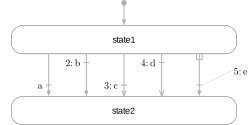
\includegraphics[width=4.85417in,height=3.42708in]{statemachine}

For the 5 transitions above, the settings are as follows, from left to
right: immediate = true, false, true, false, true; reset = true, true,
false, false, true; synchronize = false, false, false, false, true;
priority = 1, 2, 3, 4, 5. The recommended color is \{95, 95, 95\} for
states and for transition text and \{175,175,175\} for transition
lines.
\end{nonnormative}

The annotation for graphics of \lstinline!transition! has the following
structure: \lstinline!annotation(Line($\ldots$), Text($\ldots$))!; and for
\lstinline!initialState()!: \emph{graphical-primitives}\lstinline!(Line($\ldots$))!; with \lstinline!Line!
and \lstinline!Text! annotations defined in \cref{annotations}.

\begin{example}
\begin{lstlisting}[language=modelica]
transition(state2, state1, x < 10, immediate=true, reset=true, synchronize=false, priority=1)
  annotation (
    Line(
      points={{-40,-16},{-36,-4},{-32,8},{-40,26},{-40,32},{-46,50}},
      color={175,175,175},
      thickness=0.25,
      smooth=Smooth.Bezier),
    Text(
      string="%condition",
      extent={{4,-4},{4,-10}},
      fontSize=10,
      textStyle={TextStyle.Bold},
      textColor={95,95,95},
      horizontalAlignment=TextAlignment.Left),
);
\end{lstlisting}
\end{example}

The Text annotation representing the transition condition can use the
notation \%condition to refer to the condition expression.

The extent of the Text is interpreted relative to either the first point
of the Line, in the case of immediate=false, or the last point
(immediate=true).

In addition to the line defined by the points of the Line annotation, a
perpendicular line is used to represent the transition. This line is
closer to the first point if immediate=false otherwise closer to the
last point.

If the condition text is somewhat distant from the perpendicular line, a
dimmed straight line joins the transition text and the perpendicular
line.  (See the rightmost transition above.)

If \lstinline!reset=true!, a filled arrow head is used otherwise an open arrow head.
For \lstinline!synchronize=true!, an inverse ``fork'' symbol is used in the
beginning of the arrow.  (See the rightmost transition above.)

The value of the \lstinline!priority! attribute is prefixing the condition text
followed by a colon if \lstinline!priority! \textgreater{} 1.

The \lstinline!initialState! line has a filled arrow head and a bullet at the
opposite end of the initial state (as shown above).

\section{State Machine Semantics}\label{state-machine-semantics}

For the purpose of defining the semantics of state machines, assume that
the data of all transitions are stored in an array of records:
\begin{lstlisting}[language=modelica]
record Transition
  Integer from;
  Integer to;
  Boolean immediate = true;
  Boolean reset = true;
  Boolean synchronize = false;
  Integer priority = 1;
end Transition;
\end{lstlisting}

The transitions are sorted with lowest priority number last in the
array; and the priorities must be unique for each value of \lstinline!from!. The
states are enumerated from 1 and up. The transition conditions are
stored in a separate array \lstinline!c[:]! since they are time varying.

The semantics model is a discrete-time system with inputs \{\lstinline!c[:]!,
\lstinline!active!, \lstinline!reset!\} with \lstinline!t! being an array corresponding to the inputs to the
transition operator, outputs \{\lstinline!activeState!, \lstinline!activeReset!,
\lstinline!activeResetStates[:]!\} and states \{\lstinline!nextState!, \lstinline!nextReset!,
\lstinline!nextResetStates[:]!\}. For a top level state machine, active is
always true. For sub-state machines, active is true only when the parent
state is active. For a top level state machine, reset is true at the
first activation only. For sub-state machine, reset is propagated from
the state machines higher up.

\subsection{State Activation}\label{state-activation}

The state update starts from \lstinline!nextState!, i.e., what has been determined to be the next state at the previous time.
\lstinline!selectedState! takes into account if a reset of the state machine is to be done.

\begin{lstlisting}[language=modelica]
output Integer selectedState = if reset then 1 else previous(nextState);
\end{lstlisting}
The integer fired is calculated as the index of the transition to be
fired by checking that \lstinline!selectedState! is the from-state and the condition
is true for an immediate transition or previous(condition) is true for a
delayed transition. The max function returns the index of the transition
with highest priority or 0.

\begin{lstlisting}[language=modelica]
Integer fired =
  max(
    if (if t[i].from == selectedState
        then (if t[i].immediate then c[i] else previous(c[i]))
        else false)
      then i
      else 0
    for i in 1:size(t,1));
\end{lstlisting}
The start value of c is false. This definition would require that the
previous value is recorded for all transitions conditions. Below is
described an equivalent semantics which just require to record the value
of one integer variable delayed.

The integer immediate is calculated as the index of the immediate
transition to potentially be fired by checking that \lstinline!selectedState! is the
from-state and the condition is true. The max function returns the index
of the transition with true condition and highest priority or 0.

\begin{lstlisting}[language=modelica]
Integer immediate =
  max(
    if (if t[i].immediate and t[i].from == selectedState
        then c[i]
        else false)
      then i
      else 0
    for i in 1:size(t,1));
\end{lstlisting}

In a similar way, the \lstinline!Integer delayed! is calculated as the index for a
potentially delayed transition, i.e.\ a transition taking place at the
next clock tick. In this case the from-state needs to be equal to
\lstinline!nextState!:
\begin{lstlisting}[language=modelica]
Integer delayed =
  max(
    if (if not t[i].immediate and t[i].from == nextState
        then c[i]
        else false)
      then i
      else 0
    for i in 1:size(t,1));
\end{lstlisting}

The transition to be fired is determined as follows, taking into account
that a delayed transition might have higher priority than an immediate:
\begin{lstlisting}[language=modelica]
Integer fired = max(previous(delayed), immediate);
\end{lstlisting}
\lstinline!nextState! is set to the found transitions to-state:
\begin{lstlisting}[language=modelica]
Integer nextState =
  if active then
    (if fired > 0
		  then t[fired].to
		  else selectedState)
	else
    previous(nextState);
\end{lstlisting}
In order to define synchronize transitions, each state machine must
determine which are the final states, i.e.\ states without
from-transitions and to determine if the state machine is in a final
state currently:
\begin{lstlisting}[language=modelica]
Boolean finalStates[nStates] = {
  max(if  t[j].from == i then 1 else 0 for j in 1:size(t,1)) == 0
  for i in 1:nStates};
Boolean stateMachineInFinalState = finalStates[activeState];
\end{lstlisting}
To enable a synchronize transition, all the stateMachineInFinalState
conditions of all state machines within the meta state must be true. An
example is given below in the semantic example model.

\subsection{Reset Handling}\label{reset-handling}

A state can be reset for two reasons:
\begin{itemize}
\item
  The whole state machine has been reset from its context.\\
  In this case, all states must be reset, and the initial state becomes
  active.
\item
  A reset transition has been fired.\\
  Then, its target state is reset, but not other states.
\end{itemize}

The first reset mechanism is handled by the activeResetStates and
nextResetStates vectors.

The state machine reset flag is propagated and maintained to each state
individually:
\begin{lstlisting}[language=modelica]
output Boolean activeResetStates[nStates] = {if reset then true else previous(nextResetStates[i]) for i in 1:nStates};
\end{lstlisting}
until a state is eventually executed, then its corresponding reset
condition is set to false:
\begin{lstlisting}[language=modelica]
Boolean nextResetStates[nStates] =
  if active then
    {if activeState == i then false else activeResetStates[i] for i in 1:nStates}
  else
    previous(nextResetStates)
\end{lstlisting}
The second reset mechanism is implemented with the selectedReset~and
nextReset~variables. If no reset transition is fired, the nextReset is
set to false for the next cycle.

\subsection{Activation handling}\label{activation-handling}

The execution of a sub-state machine has to be suspended when its
enclosing state is not active. This activation flag is given as a
\lstinline!Boolean! input \lstinline!active!. When this flag is true, the sub-state machine
maintains its previous state, by guarding the equations of the state
variables \lstinline!nextState!, \lstinline!nextReset! and \lstinline!nextResetStates!.

\subsection{Semantics Summary}\label{semantics-summary}

The entire semantics model is given below:
\begin{lstlisting}[language=modelica]
model StateMachineSemantics "Semantics of state machines"
  parameter Integer nStates;
  parameter Transition t[:] "Array of transition data sorted in priority";
  input
  Boolean c[size(t,1)] "Transition conditions sorted in priority";
  input Boolean active "true if the state machine is active";
  input Boolean reset "true when the state
machine should be reset";
  Integer selectedState = if reset then 1 else previous(nextState);
  Boolean selectedReset = if reset then true else previous(nextReset);
  // For strong (immediate) and weak (delayed) transitions
  Integer immediate = max(if (if t[i].immediate and t[i].from == selectedState
    then c[i] else false) then i else 0 for i in 1:size(t,1));
  Integer delayed = max(if  (if not t[i].immediate and t[i].from == nextState
    then c[i] else false) then i else 0 for i in 1:size(t,1));
  Integer fired = max(previous(delayed), immediate);
  output Integer activeState = if reset then 1 elseif fired > 0 then t[fired].to else selectedState;
  output Boolean activeReset = if reset then true elseif fired > 0 then t[fired].reset else selectedReset;

  // Update states
  Integer nextState = if active then activeState else previous(nextState);
  Boolean nextReset = if active then false else previous(nextReset);
  // Delayed resetting of individual states
  output Boolean activeResetStates[nStates] = {if reset then true else
    previous(nextResetStates[i]) for i in 1:nStates};
  Boolean nextResetStates[nStates] = if active then {if activeState == i then false
    else activeResetStates[i] for i in 1:nStates} else previous(nextResetStates);
  Boolean finalStates[nStates] = {max(if  t[j].from == i then 1 else 0 for j in 1:size(t,1))== 0 for i in 1:nStates};
  Boolean stateMachineInFinalState = finalStates[activeState];
end StateMachineSemantics;
\end{lstlisting}
\subsection{Merging Variable Definitions}\label{merging-variable-definitions}

\begin{nonnormative}
When a state class uses an \lstinline!outer output! declaration,
the equations have access to the corresponding variable declared
\lstinline!inner!. Special rules are then needed to maintain the single
assignment rule since multiple definitions of such outer variables in
different mutually exclusive states needs to be merged.
\end{nonnormative}

In each state, the outer output variables are solved for and for each
such variable a single definition is formed:
\begin{lstlisting}[language=modelica,escapechar=!]
v := if activeState(state!\textsubscript{1}!) then expre!\textsubscript{1}! elseif activeState(state!\textsubscript{2}!) then expre!\textsubscript{2}! elseif ... else last(v)
\end{lstlisting}

\lstinline!last! is special internal semantic operator returning its
input. It is just used to mark for the sorting that the incidence of its
argument should be ignored. A start value must be given to the variable
if not assigned in the initial state.

A new assignment equation is formed which might be merged on higher
levels in nested state machines.

\subsection{Merging Connections to Multiple Outputs}\label{merging-connections-to-multiple-outputs}

\begin{nonnormative}
Since instances of blocks can be used as states of a state
machine it is natural to extend the connection semantics of Modelica to
allow several outputs to be connected to one input.
\end{nonnormative}

It is possible to connect several outputs to an input if all the outputs
come from states of the same state machine. In such cases, we get the
following constraint equations:
\begin{lstlisting}[language=modelica,escapechar=!]
u!\textsubscript{1}! = u!\textsubscript{2}! = ... = y!\textsubscript{1}! = y!\textsubscript{2}! = ...
\end{lstlisting}
with u\textsubscript{i} inputs and y\textsubscript{i} outputs. The
semantics is defined as follows. Introduce a variable v representing the
signal flow and rewrite the equation above as a set of equations for
u\textsubscript{i} and a set of assignment equations for v:
\begin{lstlisting}[language=modelica,escapechar=!]
v := if activeState(state!\textsubscript{1}!) then y!\textsubscript{1}! else last(v);
v := if activeState(state!\textsubscript{2}!) then y!\textsubscript{2}! else last(v);
...
u!\textsubscript{1}! = v
u!\textsubscript{2}! = v
...
\end{lstlisting}

The merge of the definitions of v is then made according to \cref{merging-variable-definitions}:
Merging Variable Definitions. The result is after
simplification:
\begin{lstlisting}[language=modelica,escapechar=!]
v := if activeState(state!\textsubscript{1}!) then y!\textsubscript{1}! elseif activeState(state!\textsubscript{2}!) then y!\textsubscript{2}! elseif ... else last(v);
u!\textsubscript{1}! = v
u!\textsubscript{2}! = v
...
\end{lstlisting}

\subsection{Example}\label{example}

\begin{example}
Consider the following hierarchical state machine:

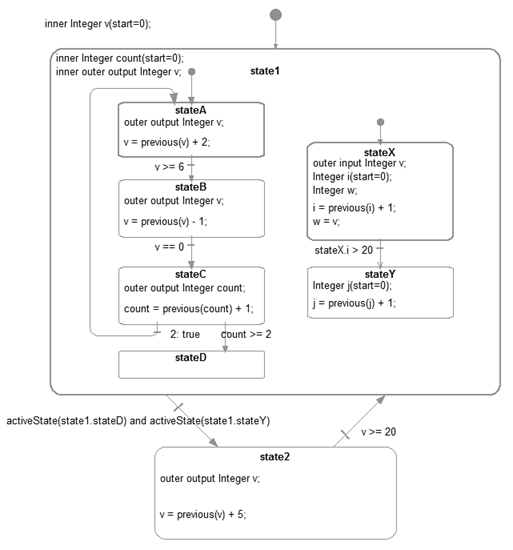
\includegraphics[width=5.34375in,height=5.72917in]{statemachine2}

The model demonstrates the following properties:
\begin{itemize}
\item
  \lstinline!state1! is a meta state with two parallel state machines in it.
\item
  \lstinline!stateA! declares \lstinline!v! as \lstinline!outer output!. \lstinline!state1! is on an intermediate
  level and declares \lstinline!v! as \lstinline!inner outer output!, i.e.\ matches lower level
  \lstinline!outer v! by being \lstinline!inner! and also matches higher level \lstinline!inner v! by being
  \lstinline!outer!. The top level declares \lstinline!v! as \lstinline!inner! and gives the start value.
\item
  \lstinline!count! is defined with a start value in \lstinline!state1!. It is reset when
  a reset transition (v\textgreater{}=20) is made to \lstinline!state1!.
\item
  \lstinline!stateX! declares the local variable \lstinline!w! to be equal to \lstinline!v! declared
  as \lstinline!inner input!.
\item
  \lstinline!stateY! declares a local counter \lstinline!j!. It is reset at start and as a
  consequence of the reset transition (v\textgreater{}=20) to \lstinline!state1!:
  When the reset transition ($v\ge 20$) fires, then the variables of the
  active states are reset immediately (so \lstinline!count! from \lstinline!state1!, and \lstinline!i!
  from \lstinline!stateX!). The variables of other states are only reset at the time
  instants when these states become active. So \lstinline!j! in \lstinline!StateY! is reset to
  0, when the transition \lstinline!stateX.i! \textgreater{} 20 fires (after \lstinline!state1!
  became active again, so after the reset transition $v\ge 20$).
\item
  Synchronizing the exit from the two parallel state machines of
  \lstinline!state1! is done by checking that \lstinline!stated! and \lstinline!stateY! are active using the
  \lstinline!activeState! function.
\end{itemize}

The Modelica code (without annotations) is:
\begin{lstlisting}[language=modelica]
block HierarchicalAndParallelStateMachine
  inner Integer v(start=0);

  State1 state1;
  State2 state2;
equation
  initialState(state1);
  transition(state1,state2,activeState(state1.stateD) and
    activeState(state1.stateY), immediate=false);
  transition(state2,state1,v >= 20, immediate=false);

public
  block State1
    inner Integer count(start=0);
    inner outer output Integer v;

    block StateA
      outer output Integer v;
    equation
      v = previous(v) + 2;
    end StateA;
    StateA stateA;

    block StateB
      outer output Integer v;
    equation
      v = previous(v) - 1;
    end StateB;
    StateB stateB;

    block StateC
      outer output Integer count;
    equation
      count = previous(count) + 1;
    end StateC;
    StateC stateC;

    block StateD
    end StateD;
    StateD stateD;

  equation
    initialState(stateA);
    transition(stateA, stateB, v >= 6, immediate=false);
    transition(stateB, stateC, v == 0, immediate=false);
    transition(stateC, stateA, true, immediate=false, priority=2);
    transition(stateC, stateD, count >= 2, immediate=false);

  public
    block StateX
      outer input Integer v;
      Integer i(start=0);
      Integer w; // = v;
    equation
      i = previous(i) + 1;
      w = v;
    end StateX;
    StateX stateX;

    block StateY
      Integer j(start=0);
    equation
      j = previous(j) + 1;
    end StateY;
    StateY stateY;

  equation
    initialState(stateX);
    transition(stateX, stateY, stateX.i > 20, immediate=false,
    reset=false);
  end State1;

  block State2
    outer output Integer v;
  equation
    v = previous(v) + 5;
  end State2;
end HierarchicalAndParallelStateMachine;
\end{lstlisting}

\Cref{fig:state-machine-behavior} shows the behavior of the state machine.
\begin{figure}[H]
  \begin{center}
    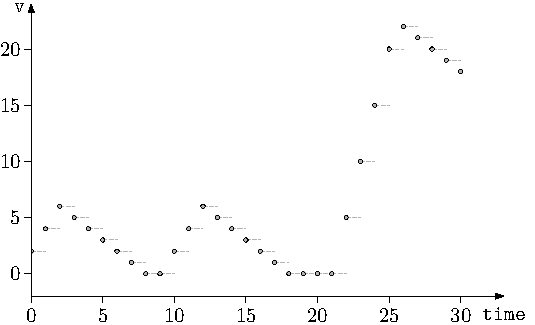
\includegraphics[width=4.16667in,height=2.91667in]{statemachineplot}
  \end{center}
  \caption{State machine behavior, as reflected by the variable \lstinline!v!.}
  \label{fig:state-machine-behavior}
\end{figure}

The transition from \lstinline!state1! to \lstinline!state2! could have been done with a
\lstinline!synchronize! transition with \lstinline!condition=true! instead. The semantically
equivalent model is shown below:
\begin{lstlisting}[language=modelica]
block HierarchicalAndParallelStateMachine
  extends StateMachineSemantics(
    nStates=2,
    t={Transition(from=1, to=2, immediate=false, synchronize=true),
       Transition(from=2, to=1, immediate=false)},
    c={true, v >= 20});
  Boolean init(start=true) = sample(false);

  block State1
    Boolean active;
    Boolean reset;
    outer input Integer v_previous;
    inner output Integer v;
    inner Integer count(start=0);
    inner Integer count_previous = if reset then 0 else previous(count);

    block StateMachineOf_stateA
      extends StateMachineSemantics(
        nStates=4,
        t={Transition(from=1, to=2, immediate=false),
           Transition(from=2, to=3, immediate=false),
           Transition(from=3, to=1, immediate=false),
           Transition(from=3, to=4, immediate=false)},
        c={v >= 6, v==0, true, count >= 2});
      outer input Integer v_previous;
      outer output Integer v;
      outer input Integer count_previous;
      outer output Integer count;
    equation
      inFinalState = true; // no macro states
      if activeState == 1 then
        // equations for stateA
        v = v_previous + 2;
        count = count_previous;
      elseif activeState == 2 then
        // equations for stateB
        v = v_previous - 1;
        count = count_previous;
      elseif activeState == 3 then
        // equations for stateC
        v = v_previous;
        count = count_previous + 1;
      else // if activeState == 4 then
        // equations for stateD
        v = v_previous;
        count = count_previous;
      end if;
    end StateMachineOf_stateA;

    StateMachineOf_stateA stateMachineOf_stateA(active=active,
      reset=reset);

    block StateMachineOf_stateX
      extends StateMachineSemantics(
        nStates=2,
        t={Transition(from=1, to=2, immediate=false, reset=false)},
        c={i>25});
      outer input Integer v;
      Integer i(start=0);
      Integer i_previous;
      Integer j(start=0);
      Integer j_previous;
      Integer w;
    equation
      inFinalState = true; // no macro states
      if activeState == 1 then
        // equations for stateX
        i_previous = if activeReset or
          activeResetStates[1] then 0 else previous(i);
        j_previous = previous(j);
        i = i_previous + 1;
        w = v;
        j = j_previous;
      else // if activeState == 2 then
        // equations for stateY
        i_previous = previous(i);
        j_previous = if activeReset or activeResetStates[2] then 0 else previous(j);
        i = i_previous;
        w = previous(w);
        j = j_previous + 1;
      end if;
    end StateMachineOf_stateX;

    StateMachineOf_stateX stateMachineOf_stateX(active=active,
      reset=reset);
    Boolean inFinalState = stateMachineOf_stateA.stateMachineInFinalState and
      stateMachineOf_stateX.stateMachineInFinalState;
  end State1;

  State1 state1;
  Integer v(start=0);
  inner Integer v_previous = if reset then 0 else previous(v);
equation
  active = true;
  reset = previous(init);
  if activeState == 1 then
    // equations for state1
    inFinalState = state1.inFinalState;
    state1.active = true;
    state1.reset = activeReset or activeResetStates[1];
    v = state1.v;
  else // if activeState == 2 then
    // equations for state2
    inFinalState = true; // not macro state
    state1.active = false;
    state1.reset = false;
    v = previous(v) + 5;
  end if;
end HierarchcialAndParallelStateMachine;
\end{lstlisting}
\end{example}


% Annotations
\chapter{Annotations}\label{annotations}

Annotations are intended for storing extra information about a model, such as graphics, documentation or versioning, etc.
A Modelica tool is free to define and use other annotations, in addition to those defined here, according to \cref{vendor-specific-annotations}.

Annotations are optional in the Modelica grammar, and when present, indicated using the \lstinline!annotation!\indexinline{annotation} keyword, see \lstinline[language=grammar]!annotation-clause! in the grammar (\cref{expressions1}).
The structure of the annotation content is the same as a class modification (\lstinline[language=grammar]!class-modification! in the grammar).
(For replaceable class declarations with a \lstinline[language=grammar]!constraining-clause! also refer to \cref{constraining-clause-annotations}.)
The specification in this document defines the semantic meaning if a tool implements any of these annotations.

\section{Vendor-Specific Annotations}\label{vendor-specific-annotations}

A vendor may -- anywhere inside an annotation -- add specific, possibly undocumented, annotations which are not intended to be interpreted by other tools.
The only requirement is that any tool shall save files with all vendor-specific annotations (and all annotations from this chapter) intact.
Two variants of vendor-specific annotations\index{vendor-specific annotation} exist; one simple and one hierarchical.
Double underscore concatenated with a vendor name as initial characters of the identifier are used to identify vendor-specific annotations.

\begin{example}
\begin{lstlisting}[language=modelica]
annotation(
  Icon(coordinateSystem(extent = {{-100, -100}, {100, 100}}),
       graphics = {__NameOfVendor(Circle(center = {0, 0}, radius = 10))}));
\end{lstlisting}
This introduces a new graphical primitive \lstinline!Circle! using the
hierarchical variant of vendor-specific annotations.
\begin{lstlisting}[language=modelica]
annotation(
  Icon(coordinateSystem(extent = {{-100, -100}, {100, 100}}),
       graphics = {Rectangle(extent = {{-5, -5}, {7, 7}},
                             __NameOfVendor_shadow = 2)}));
\end{lstlisting}
This introduces a new attribute \lstinline!__NameOfVendor_shadow!
for the \lstinline!Rectangle! primitive using the simple variant of
vendor-specific annotations.
\end{example}

\section{Annotations for Documentation}\label{annotations-for-documentation}

The \fmtannotationindex{Documentation} annotation has the following contents, where the \lstinline!info! and \lstinline!revisions! annotations are described in \cref{annotation-info-revisions}, and the \lstinline!figures! annotation is described in \cref{annotations-for-figures}:
\begin{lstlisting}[language=modelica]
record Documentation
  String info = "" "Description of the class";
  String revisions = "" "Revision history";
  Figure[:] figures = {}; "Simulation result figures";
end Documentation;
\end{lstlisting}

How the tool interprets the information in \lstinline!Documentation! is unspecified.

\subsection{Class Description and Revision History}\label{annotation-info-revisions}

Inside the \lstinline!Documentation! annotation, the \lstinline!info! annotation gives a textual description of the class, and the \lstinline!revisions! annotation gives a revision history.

\begin{nonnormative}
The \lstinline!revisions! documentation may be omitted in printed documentation.
\end{nonnormative}

If the string starts with the tag \lstinline!<html>! or \lstinline!<HTML>! the entire string is HTML encoded (and is assumed to end with \lstinline!</html>! or \lstinline!</HTML>! and shall be rendered as HTML even if the end-tags are missing), otherwise the entire string is rendered as is.  The HTML encoded content may contain links.  For external links, see \cref{external-resources}.  Links to Modelica classes may be defined with the HTML link command using scheme \lstinline!Modelica! (using its lower case form in the URI, see \cref{external-resources}), e.g.,
\begin{lstlisting}[language=modelica]
<a href="modelica://MultiBody.Tutorial">MultiBody.Tutorial</a>
\end{lstlisting}

Together with scheme \lstinline!Modelica! the (URI) fragment specifiers
\lstinline!#diagram!, \lstinline!#info!, \lstinline!#text!, \lstinline!#icon! may be used to reference different
layers. User-defined fragment specifiers (anchors) may also be used, and they may be renamed
when generating HTML (in particular to avoid collisions).
Example:
\begin{lstlisting}[language=modelica]
<a href="modelica://MultiBody.Joints.Revolute#info">Revolute</a>
\end{lstlisting}

\subsection{Annotations for Figures}\label{annotations-for-figures}

Inside the \lstinline!Documentation! annotation, each element of the \lstinline!figures! annotation array has the following content:
\begin{lstlisting}[language=modelica]
record Figure
  String title = "" "Title meant for display";
  String identifier = "" "Identifier meant for programmatic access";
  String group = "" "Name of plot group";
  Boolean preferred = false "Automatically display figure after simulation";
  Plot[:] plots "Plots";
  String caption = "" "Figure caption";
end Figure;
\end{lstlisting}

A \fmtannotationindex{Figure} is a graphical container that can contain several \lstinline!plots! described by \fmtannotationindex{Plot} annotations:
\begin{lstlisting}[language=modelica]
record Plot
  String title "Title meant for display";
  String identifier = "" "Identifier meant for programmatic access";
  Curve[:] curves "Plot curves";
  Axis x "X axis properties";
  Axis y "Y axis properties";
end Plot;
\end{lstlisting}

A \lstinline!Plot! can contain several \lstinline!curves!, see \cref{plot-curves}, that all share a common \lstinline!x! and \lstinline!y! axis with properties described in \cref{axis-properties}.

Both \lstinline!Figure! and \lstinline!Plot! can have an optional title. When
the \lstinline!Figure! \lstinline!title! is the empty string (the default), the
tool must produce a non-empty title based on the figure content.  On the other
hand, the \lstinline!Plot! \lstinline!title! has a tool-dependent default, but
the default may be the empty string.  When the \lstinline!Plot! \lstinline!title! is the empty string, no
title should be shown. The plot title is not to be confused with the plot
\emph{label} which is never empty, see below. Variable replacements, as
described in \cref{variable-replacements}, can be used in the
\lstinline!title! of \lstinline!Figure! and \lstinline!Plot!.

The \lstinline!identifier! in \lstinline!Figure! and \lstinline!Plot! is a \lstinline!String! identifier, and is intended to identify the \lstinline!Figure! and \lstinline!Plot! for programmatic access.
The \lstinline!figures! annotation is inherited in the sense that each class has a collection of figures comprised by the contents of the \lstinline!figures! annotation in the class itself, as well as the \lstinline!figures! annotations from any base classes.
A \lstinline!Figure! must be uniquely identified by its \lstinline!identifier! and a class having it in its collection.
This means that a \lstinline!Figure! \lstinline!identifier! must be unique among all \lstinline!Figure! annotations within the same \lstinline!figures! annotation as well as among all \lstinline!figures! annotations from inherited classes.
A \lstinline!Plot! \lstinline!identifier! on the other hand is only required to be unique among the \lstinline!plots! in the the same \lstinline!Figure! annotation.
If an \lstinline!identifier! is an empty string it cannot be used for programmatic access and is exempt from the uniqueness requirements.

\begin{nonnormative}
For \lstinline!Figure!, this makes it possible to reference the plot from a
tool-specific scripting environment. For \lstinline!Plot!, this makes it
possible to reference the plot in the figure caption, which becomes useful when
the \lstinline!Figure! contains more than one \lstinline!Plot!.
\end{nonnormative}

% henrikt-ma 2020-06: Once there is Modelica URI support for referring to a figure in the collection of a class, it will be easier to explain
% the following statement.
Even though a \lstinline!Figure! annotation can be shared through inheritance between classes in a class hierarchy, note that each simulated class provides
its own data to be displayed in the figure.

Every \lstinline!Plot! has an automatically generated \emph{label} which is
required to be shown as soon as at least one \lstinline!Plot! in the
\lstinline!Figure! has an \lstinline!identifier!.  A tool is free to choose both
labeling scheme (such as \emph{a}, \emph{b}, \dots, or \emph{i}, \emph{ii}, \dots), placement in the plot,
and styling in the plot itself as well as in other contexts.

When a \lstinline!Figure! defines a non-empty \lstinline!group!, it is used to
organize figures similar to how \lstinline!group! is used in the
\lstinline!Dialog! annotation (see \cref{annotations-for-the-graphical-user-interface}).  However, leaving \lstinline!group! at
the default of an empty string does not mean that a group will be created
automatically, but that the figure resides outside of any group. The
\lstinline!group! is both the key used for grouping, and the name of the group
for display purposes.

The \lstinline!preferred! attribute of \lstinline!Figure! indicates whether the figure should be given preference when automatically determining which figures to show,
and a class may define any number of \lstinline!preferred! figures.  For example, a tool might choose to automatically show all preferred figures when the class is simulated.

The \lstinline!caption! attribute of \lstinline!Figure! can use the restricted
form of text markup described in \cref{text-markup-in-captions} as well as
the variable replacements described in \cref{variable-replacements}.

\subsubsection{Axis Properties}\label{axis-properties}

Properties may be defined for each \lstinline!Plot! axis\annotationindex{Axis}:
\begin{lstlisting}[language=modelica]
record Axis
  Real min "Axis lower bound, in 'unit'";
  Real max "Axis upper bound, in 'unit'";
  String unit = "" "Unit of axis tick labels";
  String label "Axis label";
end Axis;
\end{lstlisting}

When an axis bound is not provided, the tool computes one automatically.

An empty \lstinline!unit! means that the axis is unitless, and each expression plotted against it may use its own unit determined by the tool.  The tool is responsible for conveying the information
about choice of unit for the different variables, for instance by attaching this information to curve legends.

The Modelica tool is responsible for showing that values at the axis tick marks are expressed in \lstinline!unit!, so the axis \lstinline!label! shall not contain this information.

\begin{nonnormative}
When \lstinline!unit! is empty, and axis bounds are to be determined automatically, a natural choice of unit could be the variable's \lstinline!displayUnit!.  When axis bounds are specified by the
user, on the other hand, a tool may choose a unit for the variable such that the range of the variable values (expressed in the chosen unit) fit nicely with the range of the unitless axis.
\end{nonnormative}

If a tool does not recognize the \lstinline!unit!, it is recommended to issue a warning and treat the \lstinline!unit! as if it was empty, as well as ignore any setting for \lstinline!min! and \lstinline!max!.

When \lstinline!label! is not provided, the tool produces a default label.
Providing the empty string as \lstinline!label! means that no label should be shown.
Variable replacements, as described in \cref{variable-replacements}, can be used in \lstinline!label!.
The Modelica tool is responsible for showing the unit used for values at the axis tick marks, so the axis \lstinline!label! shall not contain the unit.

\subsubsection{Plot Curves}\label{plot-curves}

The actual data to plot is specified in the \lstinline!curves!\annotationindex{Curve} of a \lstinline!Plot!:
\begin{lstlisting}[language=modelica]
record Curve
  expression x = time "X coordinate values";
  expression y "Y coordinate values";
  String legend "Legend";
end Curve;
\end{lstlisting}

The mandatory \lstinline!x! and \lstinline!y! expressions are restricted to be component references referring to a scalar variable or \lstinline!time!.
It is an error if \lstinline!x! or \lstinline!y! does not designate a scalar variable.
When the \lstinline!unit! of an \lstinline!Axis! is non-empty, it is an error if the unit of the corresponding \lstinline!x! or \lstinline!y! expression (i.e., a variable's \lstinline!unit!, or second for \lstinline!time!) is incompatible with the axis unit.

When \lstinline!legend! is not provided, the tool produces a default based on \lstinline!x! and/or \lstinline!y!.
Providing the empty string as \lstinline!legend! means that the curve shall be omitted from the plot legend.
Variable replacements, as described in \cref{variable-replacements}, can be used in \lstinline!legend!.

\subsubsection{Escape sequences}\label{text-markup-escape-sequences}

In an attribute inside a figure where the variable replacements of \cref{variable-replacements} or the text markup of \cref{text-markup-in-captions} can be used, the following use of \firstuse{text markup escape sequences}\index{text markup escape sequence}\index{escape sequence!text markup} applies.
These escape sequences are applied after the application of other markup, and is not applied at all inside some of the other markup, see details for the respective markup.

The percent character `\%' shall be encoded \lstinline!%%!.  The following are all the recognized escape sequences:
\begin{center}
\begin{tabular}{c c l}
\hline
\tablehead{Sequence} & \tablehead{Encoded character} & \tablehead{Comment}\\
\hline
\hline
\lstinline!%%! & `\%' & Only way to encode character. \\
\lstinline!%]! & `]'  & Prevents termination of markup delimited by \lstinline![$\ldots$]!. \\
\hline
\end{tabular}
\end{center}

\begin{nonnormative}
With the percent character being encoded as \lstinline!%%!, the behavior of \lstinline!%! appearing in any other way than the escape sequences above, for variable replacement (\cref{variable-replacements}), or for the text markup (\cref{text-markup-in-captions}) is undefined, and thus possible to define in the future without breaking backward compatibility.
\end{nonnormative}

\subsubsection{Variable Replacements}\label{variable-replacements}

In the places listed in \cref{attributes-with-variable-replacements} where text for display is defined, the final value of a result variable can be embedded by referring to the variable as \lstinline!%{inertia1.w}!.
This is similar to the \lstinline!Text! graphical primitive in \cref{text}.

\begin{table}[H]
\caption{Attributes that can use variable replacements.}
\label{attributes-with-variable-replacements}
\begin{center}
\begin{tabular}{l l}
\hline
\tablehead{Attribute} & \tablehead{Annotation}\\
\hline
\hline
\lstinline!title! & \lstinline!Figure! and \lstinline!Plot! \\
\lstinline!caption! & \lstinline!Figure! \\
\lstinline!legend! & \lstinline!Curve! \\
\lstinline!label! & \lstinline!Axis! \\
\hline
\end{tabular}
\end{center}
\end{table}

In \lstinline!%{$\mathit{variable}$}!, text markup escape sequences don't apply inside the $\mathit{variable}$, which has the form of \lstinline[language=grammar]!component-reference! in the grammar (\cref{expressions1}).  This means that a complete \lstinline[language=grammar]!component-reference! shall be scanned before looking for the terminating closing brace.

\begin{example}
The variable replacement \lstinline!%{'%%'}! references the variable \lstinline!'%%'!, not the variable \lstinline!'%'!.
\end{example}

\begin{example}
The variable replacement \lstinline!%{foo . '}bar{'}! makes a valid reference to the variable\linebreak[4] \lstinline!foo.'}bar{'!.
\end{example}

Note that expansion to the final value means that expansion is not restricted to
parameters and constants, so that values to be shown in a caption can be
determined during simulation.

\begin{nonnormative}
By design, neither \lstinline!%class! nor \lstinline!%name! is supported in this context, as this information is expected to already be easily accessible (when applicable) in tool-specific ways.  (Titles making use of \lstinline!%class! or \lstinline!%name! would then only lead to ugly duplication of this information.)
\end{nonnormative}

\subsubsection{Text Markup in Captions}\label{text-markup-in-captions}

In addition to variable replacements, a very restricted form of text markup is used for the \lstinline!caption!.  Note that the text markup escape sequences described in \cref{text-markup-escape-sequences} generally apply inside \lstinline!caption!, with one exception given below for links.

Links take the form \lstinline!%[$\mathit{text}$]($\mathit{link}$)!, where the \lstinline![$\mathit{text}$]! part is optional, and text markup escape sequences don't apply inside the $\mathit{link}$.  The $\mathit{link}$ can be in either of the following forms, where the interpretation is given by the first matching form:
\begin{itemize}
\item
A \lstinline!variable:$\mathit{id}$!, where $\mathit{id}$ is a component reference in the form of \lstinline[language=grammar]!component-reference! in the grammar, such as \lstinline!inertia1.w!.
\item
% The 'plot:id' form below should be deprecated in favor of using an improved form of Modelica URI reference in the future, making 'variable:id' the only non-URI reference.
A \lstinline!plot:$\mathit{id}$!, where $\mathit{id}$ is the identifier of a \lstinline!Plot! in the current \lstinline!Figure!.
\item
% Use very short Modelica URI combined with carefully chosen wording below to deal with difficult line breaking.
A URI.
Well established schemes such as \lstinline[language={[nocomment]modelica}]!https://github.com/modelica! or \lstinline[language={[nocomment]modelica}]!modelica://Modelica!, as well as lesser known schemes may be used.
(A tool that has no special recognition of a scheme can try sending the URI to the operating system for interpretation.)
\end{itemize}

When \lstinline![$\mathit{text}$]! is omitted, a Modelica tool is free to derive a default based on the $\mathit{link}$.

\begin{nonnormative}
Note that for the character `]' to appear in $\mathit{text}$, it needs to be encoded as the escape sequence \lstinline!%]!, or it would be interpreted as the terminating delimiter of the \lstinline![$\mathit{text}$]!.

Similarly, the closing parenthesis `)' must be handled with care in $\mathit{link}$ in order to not be interpreted as the terminating delimiter of the \lstinline!($\mathit{link}$)!.
\begin{itemize}
\item
For a \lstinline!variable:!, no special treatment is needed, as the component reference syntax of the $\mathit{id}$ allows parentheses to appear without risk of misinterpretation inside a quoted identifier.
For example, \lstinline"%(variable:'try)me!')" has a parenthesis in \lstinline"'try)me!'" that must not be mistaken for the end of the \lstinline!($\mathit{link}$)!.
% The following shortcoming would be resolved if the 'plot:id' form was replaced by a Modelica URI reference, thanks to URL encoding.
\item
For a \lstinline!plot:!, there is currently no way to reference a plot with `)' in its \lstinline!identifier!.
\item
For a URI, a closing parenthesis must be URL encoded in order to not be interpreted as the end of the \lstinline!($\mathit{link}$)!.
For example, the URL in \lstinline[language={[nocomment]modelica}]!%(http://example.org/(tryme))! is just \filename{http://example.org/(tryme}, and the entire link is followed by a stray closing parenthesis.
To make it work, one has to use URL encoding: \lstinline[language={[nocomment]modelica}]!%(http://example.org/%28tryme%29)! (using URL encoding of the opening parenthesis just for symmetry, and note that the \lstinline!%! of the percent-encoded sequences are not subject to text markup escape sequences).
\end{itemize}
\end{nonnormative}

The styling of the link text, as well as the link action, is left for each Modelica
tool to decide.

\begin{nonnormative}
For example, \lstinline!%(inertia1.w)! could be displayed as the text
\lstinline!inertia1.w! formatted with upright monospaced font, and have a pop-up
menu attached with menu items for plotting the variable, setting its start
value, or investigating the equation system from which it is solved.  On the
other hand, \lstinline!%[angular velocity](inertia1.w)! could be formatted in
the same style as the surrounding text, except some non-intrusive visual clue
about it being linked.
\end{nonnormative}

\begin{nonnormative}
% This non-normative text explains why we don't want to assume that the 'link' must have a scheme.
Note that $\mathit{link}$ is currently not allowed to be a \emph{URI reference}, i.e., a URI or a \emph{relative reference} such as \lstinline!#foo!.  This is due to to the current inability to define a base URI referencing the current figure.  Once this becomes possible, the URI form of $\mathit{link}$ may be changed into a URI reference.
\end{nonnormative}

A sequence of one or more newlines (encoded either literally or using the \lstinline!\n!
escape sequence) means a paragraph break.  (A line break within a paragraph is
not supported, and any paragraph break before the first paragraph or after the last
paragraph has no impact.)

\firstuse{Vendor-specific markup}\index{vendor-specific markup} takes the form \lstinline!%__$\mathit{nameOfVendor}_{1}$($\mathit{data}_{1}$)$\ldots$__$\mathit{nameOfVendor}_{n}$($\mathit{data}_{n}$)[$\mathit{text}$]!, where $n \geq 1$.
The $\mathit{nameOfVendor}$ consists of only digits and letters, and shall only convey the name of the vendor defining the meaning of the associated $\mathit{data}$.
Text markup escape sequences don't apply inside the $\mathit{data}$, implying that it cannot contain the closing parenthesis, `)'.
A tool which does not understand any of the vendor-specific meanings shall only display the mandatory $\mathit{text}$, but the $\mathit{text}$ may also be used together with the vendor-specific $\mathit{data}$.

\begin{example}
One application of vendor-specific markup is to prototype a feature that can later be turned into standardized markup.  For example, say that the tool AVendor wants to generalize the variable replacements such that the duration of a simulation can be substituted into a caption.  During the development, this could be represented as the vendor-specific markup \lstinline!%__AVendor(?duration)[10 s]!, if the simulation has a duration of 10~seconds at the time of writing the caption.  When AVendor renders this, it ignores the text \lstinline!10 s! and just displays the actual duration instead.  Later, if this would become supported by standard markup, it might take the form of something like \lstinline!%{experiment:duration}! instead (note that \lstinline!experiment:duration! is not in the form of a component reference, avoiding conflict with current use of variable replacements).

In a similar way, vendor-specific markup can be used to prototype a link for future inclusion in the link markup (either by extending the meaning of Modelica URIs, or by introducing another pseudo-scheme similar to \lstinline!variable:!).  This is an example where the vendor-specific markup could make use of the $\mathit{text}$ (for link text) together with the vendor-specific $\mathit{data}$ (describing the actual link).
\end{example}

\section{Annotations for Symbolic Processing}\label{annotations-for-symbolic-processing}

The annotation listed below, in addition to annotations described in \crefrange{derivatives-and-inverses-of-functions}{function-inlining-and-event-generation}, can influence the symbolic processing.
\begin{center}
\begin{tabular}{l|l l}
\hline
\tablehead{Annotation} & \tablehead{Description} & \tablehead{Details}\\
\hline
\hline
\lstinline!Evaluate! & Use parameter value for symbolic processing & \Cref{modelica:Evaluate}\\
\hline
\end{tabular}
\end{center}

\begin{annotationdefinition}[Evaluate]
\begin{synopsis}[grammar]\begin{lstlisting}
"Evaluate" "=" ( false | true )
\end{lstlisting}\end{synopsis}
\begin{semantics}
The annotation \lstinline!Evaluate! can occur in the component declaration, its type declaration, or a base class of the type-declaration.
In the case of multiple conflicting annotations it is handled similarly to modifiers (e.g., an \lstinline!Evaluate! annotation on the component declaration takes precedence).
In the case of hierarchical components it is applied to all components, overriding any \lstinline!Evaluate!-setting for specific components.
The annotation \lstinline!Evaluate! only has effect for a component declared with the prefix \lstinline!parameter!.

If \lstinline!Evaluate = true!, the model developer proposes to utilize the value for the symbolic processing. In that case, it is not possible to change the parameter value after symbolic pre-processing.

If \lstinline!Evaluate = false!, the model developer proposes to not utilize the value of the corresponding parameter for the symbolic processing.

\begin{nonnormative}
\lstinline!Evaluate! is for example used for axis of rotation parameters in the \lstinline!Modelica.Mechanics.MultiBody! library in order to improve the efficiency of the generated code.
\end{nonnormative}
\end{semantics}
\end{annotationdefinition}


\section{Annotations for Simulations}\label{annotations-for-simulations}

The annotations listed below define how models can be checked, translated, and simulated.
\begin{center}
\begin{tabular}{l|l l}
\hline
\tablehead{Annotation} & \tablehead{Description} & \tablehead{Details}\\
\hline
\hline
\lstinline!experiment! & Simulation experiment settings & \Cref{modelica:experiment}\\
\lstinline!HideResult! & Don't show component's simulator result & \Cref{modelica:HideResult}\\
\lstinline!TestCase! & Information for model used as test case & \Cref{modelica:TestCase}\\
\hline
\end{tabular}
\end{center}

\begin{annotationdefinition}[experiment]
% henrikt-ma 2021-04: Seems strange to allow 'experiment' completely without list of options -- what would it mean?
\begin{synopsis}[grammar]\begin{lstlisting}
"experiment"
   [ "(" [ experimentOption { "," experimentOption } ] ")" ]

experimentOption:
   "StartTime" "=" [ "+" | "-" ] UNSIGNED-NUMBER
   | "StopTime" "=" [ "+" | "-" ] UNSIGNED-NUMBER
   | "Interval" "=" UNSIGNED-NUMBER
   | "Tolerance" "=" UNSIGNED-NUMBER
\end{lstlisting}\end{synopsis}
\begin{semantics}
The \lstinline{experiment} annotation defines the default start time (\lstinline!StartTime!) in {[}s{]}, the default stop time (\lstinline!StopTime!) in {[}s{]}, the suitable time resolution for the result grid (\lstinline!Interval!) in {[}s{]}, and the default relative integration tolerance (\lstinline!Tolerance!) for simulation experiments to be carried out with the model or block at hand.
If \lstinline!StartTime! is not specified it is assumed to be \lstinline!0.0!.
\end{semantics}
\end{annotationdefinition}

\begin{annotationdefinition}[HideResult]
\begin{synopsis}[grammar]\begin{lstlisting}
"HideResult" "=" ( false | true )
\end{lstlisting}\end{synopsis}
\begin{semantics}
\lstinline!HideResult = true! defines that the model developer proposes to not show the simulator results of the corresponding component.

\lstinline!HideResult = false! defines that the developer proposes to show the corresponding component.

\begin{nonnormative}
For example, a tool is not expected to provide means to plot a variable with \lstinline!HideResult = true!.  If a variable is declared in a protected section, a tool might not include it in a simulation result. By setting \lstinline!HideResult = false!, the modeler would like to have the variable in the simulation result, even if in the protected section.

\lstinline!HideResult! is for example used in the connectors of the \lstinline!Modelica.StateGraph! library to not show variables to the modeler that are of no interest to him and would confuse him.
\end{nonnormative}
\end{semantics}
\end{annotationdefinition}

\begin{annotationdefinition}[TestCase]
\begin{synopsis}[grammar]\begin{lstlisting}
"TestCase" "(" "shouldPass" "=" ( false | true ) ")"
\end{lstlisting}\end{synopsis}
\begin{semantics}
If \lstinline!shouldPass! is \lstinline!false! it indicates that the translation or the simulation of the model should fail.
If a tools checks a package where classes have \lstinline!shouldPass = false! they should not generate errors, and checking may even be skipped.
On the other hand, models with \lstinline!shouldPass = false! may be useful for creation of negative tests in tool-specific ways.
Similarly as a class with obsolete-annotation, a class with \lstinline!TestCase! annotation (regardless of the value of \lstinline!shouldPass!) shall not be used in other models, unless those models also have a \lstinline!TestCase! annotation.

\begin{nonnormative}
The intent of the test-case can be included in the documentation of the class.
This annotation can both be used for models intended as test-cases for implementations, and for models explaining detectable errors.
\end{nonnormative}
\end{semantics}
\end{annotationdefinition}


\section{Annotation for Single Use of Class}\label{annotation-for-single-use-of-class}

For state machines it is useful to have single instances of local classes.
This can be done using:
\begin{lstlisting}[language=modelica]
annotation(singleInstance = true)
\end{lstlisting}

The annotation \fmtannotationindex{singleInstance} in a class indicates that there should only be one component instance of the class, and it should be in the same scope as the class is defined.
The intent is to remove the class when the component is removed and to prevent duplication of the component.


\section{Annotations for Graphical Objects}\label{annotations-for-graphical-objects}

A graphical representation of a class consists of two abstraction
layers, icon layer and diagram layer showing graphical objects,
component icons, connectors and connection lines. The icon
representation typically visualizes the component by hiding hierarchical
details. The hierarchical decomposition is described in the diagram
layer showing icons of subcomponents and connections between these.

Graphical annotations described in this chapter ties into the Modelica
grammar as follows.
\begin{lstlisting}[language=grammar]
graphical-annotations :
  annotation "(" [ layer-annotations ] ")"

layer-annotations :
  ( icon-layer | diagram-layer ) [ "," layer-annotations ]
\end{lstlisting}
Layer descriptions (start of syntactic description):
\begin{lstlisting}[language=grammar]
icon-layer :
  "Icon" "(" [ coordsys-specification "," ] graphics ")"

diagram-layer :
  "Diagram" "(" [ coordsys-specification "," ] graphics ")"
\end{lstlisting}%
\annotationindex{Icon}\annotationindex{Diagram}

\begin{example}
\begin{lstlisting}[language=modelica]
annotation(
   Icon(coordinateSystem(extent = {{-100, -100}, {100, 100}}),
        graphics = {Rectangle(extent = {{-100, -100}, {100, 100}}),
                    Text(extent = {{-100, -100}, {100, 100}},
                         textString = "Icon")}));
\end{lstlisting}
\end{example}

The graphics is specified as an ordered sequence of graphical primitives, which are described below.
First base class contents is drawn according to the order of the \lstinline!extends!-clauses, and then graphical primitives are drawn according to the order such that later objects can cover earlier ones.

\begin{nonnormative}
Note that the ordered sequence is syntactically a valid Modelica annotation, although there
is no mechanism for defining an array of heterogeneous objects in Modelica.
\end{nonnormative}

These \lstinline!Icon!, \lstinline!Diagram!, and \lstinline!Documentation! annotations are only allowed directly in classes (e.g.\ not on components or connections).
The allowed annotations for a short class definition is the union of the allowed annotations in classes and on \lstinline!extends!-clauses.

\subsection{Common Definitions}\label{common-definitions}

The following common definitions are used to define graphical annotations in the later sections.
\begin{lstlisting}[language=modelica]
type DrawingUnit = Real(final unit="mm");
type Point = DrawingUnit[2] "{x, y}";
type Extent = Point[2] "Defines a rectangular area {{x1, y1}, {x2, y2}}";
\end{lstlisting}%
\annotationindex{DrawingUnit}\annotationindex{Point}\annotationindex{Extent}
The interpretation of \lstinline!unit! is with respect to printer output in natural size (not zoomed).

All graphical entities have a visible attribute which indicates if the entity should be shown.
\begin{lstlisting}[language=modelica]
partial record GraphicItem
  Boolean visible = true;
  Point origin = {0, 0};
  Real rotation(quantity="angle", unit="deg")=0;
end GraphicItem;
\end{lstlisting}%
\annotationindex{GraphicItem}
The \lstinline!origin! attribute specifies the origin of the graphical item in the coordinate system of the layer in which it is defined.
The origin is used to define the geometric information of the item and for all transformations applied to the item.
All geometric information is given relative the \lstinline!origin! attribute, which by default is \lstinline!{0, 0}!.

The \lstinline!rotation! attribute specifies the rotation of the graphical item
counter-clockwise around the point defined by the \lstinline!origin! attribute.

\subsubsection{Coordinate Systems}\label{coordinate-systems}

Each of the layers has its own coordinate system.\annotationindex{CoordinateSystem}
A coordinate system is defined by the coordinates of two points, the left (x1) lower (y1) corner and the right (x2) upper (y2) corner, where the coordinates of the first point shall be less than the coordinates of the second point.

The attribute \lstinline!preserveAspectRatio! specifies a hint for the shape of
components of the class, but does not actually influence the rendering of the component.
If \lstinline!preserveAspectRatio! is true, changing the
extent of components should preserve the current aspect ratio of the coordinate
system of the class.

The attribute \lstinline!initialScale! specifies the default component size as
\lstinline!initialScale! times the size of the coordinate system of the class. An
application may use a different default value of \lstinline!initialScale!.

The attribute \lstinline!grid! specifies the spacing between grid points which can
be used by tools for alignment of points in the coordinate system, e.g.\ ``snap-to-grid''.
Its use and default value is tool-dependent.

\begin{lstlisting}[language=modelica]
record CoordinateSystem
  Extent extent;
  Boolean preserveAspectRatio = true;
  Real initialScale = 0.1;
  DrawingUnit grid[2];
end CoordinateSystem;
\end{lstlisting}

\begin{example}
A coordinate system for an icon could for example be defined as:
\begin{lstlisting}[language=modelica]
CoordinateSystem(extent = {{-10, -10}, {10, 10}});
\end{lstlisting}
i.e.\ a coordinate system with width 20 units and height 20 units.
\end{example}

The coordinate systems for the icon and diagram layers are by default
defined as follows; where the array of \lstinline!GraphicsItem! represents an
ordered list of graphical primitives.

\begin{lstlisting}[language=modelica]
record Icon "Representation of the icon layer"
  CoordinateSystem coordinateSystem(extent = {{-100, -100}, {100, 100}});
  GraphicItem[:] graphics;
end Icon;

record Diagram "Representation of the diagram layer"
  CoordinateSystem coordinateSystem(extent = {{-100, -100}, {100, 100}});
  GraphicItem[:] graphics;
end Diagram;
\end{lstlisting}
The coordinate system (including \lstinline!preserveAspectRatio!) of a class is defined by the following priority:
\begin{enumerate}
\item
  The coordinate system annotation given in the class (if specified).
\item
  The coordinate systems of the first base class where the extent on the \lstinline!extends!-clause specifies a null-region (if any).
  Note that null-region is the default for base classes, see \cref{extends-clause}.
\item
  The default coordinate system \lstinline!CoordinateSystem(extent = {{-100, -100}, {100, 100}})!.
\end{enumerate}

\subsubsection{Graphical Properties}\label{graphical-properties}

Properties of graphical objects and connection lines are described using the following attribute types.
\begin{lstlisting}[language=modelica]
type Color = Integer[3](min = 0, max = 255) "RGB representation";
constant Color Black = zeros(3);
type LinePattern = enumeration(None, Solid, Dash, Dot, DashDot, DashDotDot);
type FillPattern = enumeration(None, Solid, Horizontal, Vertical,
                               Cross, Forward, Backward, CrossDiag,
                               HorizontalCylinder, VerticalCylinder, Sphere);
type BorderPattern = enumeration(None, Raised, Sunken, Engraved);
type Smooth = enumeration(None, Bezier);
type EllipseClosure = enumeration(None, Chord, Radial);
\end{lstlisting}%
\annotationindex{Color}\annotationindex{LinePattern}\annotationindex{FillPattern}\annotationindex{BorderPattern}\annotationindex{Smooth}\annotationindex{EllipseClosure}
The \lstinline!LinePattern! attribute \lstinline!Solid! indicates a normal line, \lstinline!None! an invisible line, and the other attributes various forms of dashed/dotted lines.

The \lstinline!FillPattern! attributes \lstinline!Horizontal!, \lstinline!Vertical!, \lstinline!Cross!, \lstinline!Forward!, \lstinline!Backward! and \lstinline!CrossDiag! specify fill patterns drawn with the line color over the fill color.

The attributes \lstinline!HorizontalCylinder!, \lstinline!VerticalCylinder! and \lstinline!Sphere! specify
gradients that represent a horizontal cylinder, a vertical cylinder and
a sphere, respectively. The gradient goes from line color to fill color.

The border pattern attributes \lstinline!Raised!, \lstinline!Sunken! and \lstinline!Engraved! represent frames which are rendered in a tool-dependent way --- inside the extent of the filled shape.

\begin{figure}[H]
  \begin{center}
    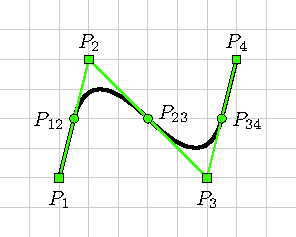
\includegraphics{bezierpoints}
  \end{center}
  \caption{Line with \lstinline!smooth = Bezier!.  The four line points $P_{1}$, \ldots{}, $P_{4}$ result in two quadratic splines and two straight line segments.}\label{fig:smooth-bezier}
\end{figure}

The \lstinline!smooth! attribute specifies that a line can be drawn as straight line segments (\lstinline!None!) or using a spline (\lstinline!Bezier!), where the line's points specify control points of a quadratic Bezier curve, see \cref{fig:smooth-bezier}.

For lines with only two points, the \lstinline!smooth! attribute has no effect.

For lines with three or more points ($P_{1}$, $P_{2}$, \ldots{}, $P_{n}$), the middle point of each line segment ($P_{12}$, $P_{23}$, \ldots{}, $P_{(n-1)n}$) becomes the starting point and ending
points of each quadratic Bezier curve.  For each quadratic Bezier curve, the common point of the two line segment becomes the control point. For instance, point $P_{2}$ becomes the control point for
the Bezier curve starting at $P_{12}$ and ending at $P_{23}$.  A straight line is drawn between the starting point of the line and the starting point of the first quadratic Bezier curve, as well as
between the ending point of the line and the ending point of the last quadratic Bezier curve.

In the illustration above, the square points ($P_{1}$, $P_{2}$, $P_{3}$, and $P_{4}$) represent the points that define the line, and the circle points ($P_{12}$, $P_{23}$, and $P_{34}$) are the
calculated middle points of each line segment.  Points $P_{12}$, $P_{2}$, and $P_{23}$ define the first quadratic Bezier curve, and the points $P_{23}$, $P_{3}$, and $P_{34}$ define the second
quadratic Bezier curve.  Finally a straight line is drawn between points $P_{1}$ and $P_{12}$ as well as between $P_{34}$ and $P_{4}$.

The values of the \lstinline!EllipseClosure! enumeration specify if and how the endpoints of an elliptical arc are to be joined (see \cref{ellipse}).

\begin{lstlisting}[language=modelica]
type Arrow = enumeration(None, Open, Filled, Half);
type TextStyle = enumeration(Bold, Italic, UnderLine);
type TextAlignment = enumeration(Left, Center, Right);
\end{lstlisting}%
\annotationindex{Arrow}\annotationindex{TextStyle}\annotationindex{TextAlignment}

Filled shapes have the following attributes for the border and interior.
\begin{lstlisting}[language=modelica]
record FilledShape "Style attributes for filled shapes"
  Color lineColor = Black "Color of border line";
  Color fillColor = Black "Interior fill color";
  LinePattern pattern = LinePattern.Solid "Border line pattern";
  FillPattern fillPattern = FillPattern.None "Interior fill pattern";
  DrawingUnit lineThickness = 0.25 "Line thickness";
end FilledShape;
\end{lstlisting}%
\annotationindex{FilledShape}
The extent/points of the filled shape describe the theoretical zero-thickness filled shape, and the actual rendered border is then half inside and half outside the extent.

\subsection{Component Instance}\label{component-instance}

A component instance can be placed within a diagram or icon layer.
It has an annotation with a \lstinline!Placement! modifier to describe the placement.
Placements are defined in term of coordinate systems transformations:
\begin{lstlisting}[language=modelica]
record Transformation
  Point origin = {0, 0};
  Extent extent;
  Real rotation(quantity = "angle", unit = "deg") = 0;
end Transformation;
\end{lstlisting}%
\annotationindex{Transformation}
The origin attribute defines the position of the component in the coordinate system of the enclosing class.
The \lstinline!extent! defines the position, size and flipping of the component, relative to the \lstinline!origin! attribute.
The \lstinline!extent! is defined relative to the \lstinline!origin! attribute of the component instance.
Given an extent \lstinline!{{$x_{1}$, $y_{1}$}, {$x_{2}$, $y_{2}$}}!, $x_{2} < x_{1}$ defines horizontal flipping and $y_{2} < y_{1}$ defines vertical flipping around the center of the object.

The \lstinline!rotation! attribute specifies rotation of the extent around the point defined by the \lstinline!origin! attribute.

The graphical operations are applied in the order: scaling, flipping and rotation.

\begin{lstlisting}[language=modelica]
record Placement
  Boolean visible = true;
  Transformation transformation "Placement in the diagram layer";

  Boolean iconVisible "Visible in icon layer; for public connector";
  Transformation iconTransformation "Placement in the icon layer; for public connector";
end Placement;
\end{lstlisting}%
\annotationindex{Placement}
If no \lstinline!iconTransformation! is given the \lstinline!transformation! is also used for placement in the icon layer.
If no \lstinline!iconVisible! is given for a public connector the \lstinline!visible! is also used for visibility in the icon layer.

\begin{nonnormative}
A connector can be shown in both an icon layer and a diagram
layer of a class. Since the coordinate systems typically are different,
placement information needs to be given using two different coordinate
systems. More flexibility than just using scaling and translation is
needed since the abstraction views might need different visual placement
of the connectors. The attribute \lstinline!transformation! gives the placement in
the diagram layer and \lstinline!iconTransformation! gives the placement in the icon
layer. When a connector is shown in a diagram layer, its diagram layer
is shown to facilitate opening up a hierarchical connector to allow
connections to its internal subconnectors.
\end{nonnormative}

For connectors, the icon layer is used to represent a connector when it
is shown in the icon layer of the enclosing model. The diagram layer of
the connector is used to represent it when shown in the diagram layer of
the enclosing model. Protected connectors are only shown in the diagram
layer. Public connectors are shown in both the diagram layer and the
icon layer. Non-connector components are only shown in the diagram
layer.

\subsection{Extends-clause}\label{extends-clause}

Each \lstinline!extends!-clause (and short class definition, as stated in \cref{annotations-for-graphical-objects}) may have layer specific annotations which describe the rendering of the base class' icon and diagram layers in the derived class.

\begin{lstlisting}[language=modelica]
record IconMap
  Extent extent = {{0, 0}, {0, 0}};
  Boolean primitivesVisible = true;
end IconMap;

record DiagramMap
  Extent extent = {{0, 0}, {0, 0}};
  Boolean primitivesVisible = true;
end DiagramMap;
\end{lstlisting}%
\annotationindex{IconMap}\annotationindex{DiagramMap}
All graphical objects are by default inherited from a base class.
If the \lstinline!primitivesVisible! attribute is false, components and connections are visible but graphical primitives are not.

\begin{itemize}
\item
  If the extent of the \lstinline!extends!-clause defines a null region (the default), the base class contents is mapped to the same coordinates in the derived class, and the coordinate system (including \lstinline!preserveAspectRatio!) can be inherited as described in \cref{coordinate-systems}.
\item
  If the extent of the \lstinline!extends!-clause defines a non-null region, the base class coordinate system is mapped to the region specified by the attribute extent, if \lstinline!preserveAspectRatio! is true for the base class the mapping shall preserve the aspect ratio.
  The base class coordinate system (and \lstinline!preserveAspectRatio!) is not inherited.
\end{itemize}

\begin{example}
\begin{lstlisting}[language=modelica]
model A
  extends B annotation(
    IconMap(extent = {{-100, -100}, {100, 100}}, primitivesVisible = false),
    DiagramMap(extent = {{-50, -50}, {0, 0}}, primitivesVisible = true)
  );
end A;

model B
  extends C annotation(DiagramMap(primitivesVisible = false));
  $\ldots$
end B;
\end{lstlisting}
In this example the diagram of \lstinline!A! contains the graphical primitives
from \lstinline!A! and \lstinline!B! (but not from \lstinline!C! since they were hidden in \lstinline!B!) -- the ones
from \lstinline!B! are rescaled, and the icon of \lstinline!A! contains the graphical primitives
from \lstinline!A! (but neither from \lstinline!B! nor from \lstinline!C!).
\end{example}

\subsection{Connections}\label{connections1}

A connection is specified with an annotation containing a \lstinline!Line!\index{Line@\robustinline{Line}!\robustinline{connect} annotation} primitive and optionally a \lstinline!Text! primitive, as specified below.

\begin{example}
\begin{lstlisting}[language=modelica]
connect(a.x, b.x)
  annotation(Line(points = {{-25, 30}, {10, 30}, {10, -20}, {40, -20}}));
\end{lstlisting}
\end{example}

The optional \lstinline!Text!\index{Text@\robustinline{Text}!\robustinline{connect} annotation} primitive defines a text that will be written on the connection line.
It has the following definition (\emph{it is not equal to the \lstinline!Text! primitive as part of graphics -- the differences are marked as bold lines}):
% NOTE: Technically just the names -- not the entire lines are marked in bold
\begin{lstlisting}[language=modelica]
record Text
  extends GraphicItem;
  extends FilledShape;
  Extent extent;
  String string;
  Real fontSize = 0 "unit pt";
  String fontName;
  TextStyle textStyle[:];
  Color textColor = lineColor;
  TextAlignment horizontalAlignment =
    if index < 0 then TextAlignment.Right else TextAligment.Left;
  Integer index;
end Text;
\end{lstlisting}

The \lstinline!index! is one of the points of Line (numbered 1, 2, 3, \ldots{} where negative numbers count from the end, thus -1 indicate the last one).
The \lstinline!string! may use the special symbols \lstinline!"%first"! and \lstinline!"%second"! to indicate the connectors in the \lstinline!connect!-equation.

The \lstinline!extent! and \lstinline!rotation! are relative to the \lstinline!origin! (default \lstinline!{0, 0}!) and the \lstinline!origin! is relative to the point on the \lstinline!Line!.

The \lstinline!textColor! attribute defines the color of the text.  The text is drawn with transparent background and no border around the text (and without outline).  The contents inherited from \lstinline!FilledShape! is deprecated, but kept for compatibility reasons.  The default value for \lstinline!horizontalAlignment! is deprecated.  Having a zero size for the \lstinline!extent! is deprecated and is handled as if upper part is moved up an appropriate amount.

\begin{example}
\begin{lstlisting}[language=modelica]
connect(controlBus.axisControlBus1, axis1.axisControlBus)
  annotation(
    Text(string = "%first", index = -1, extent = [-6, 3; -6, 7]),
    Line(points =
      {{-80,-10},{-80,-14.5},{-79,-14.5},{-79,-17},{-65,-17},{-65,-65},{-25,-65}})
  );
\end{lstlisting}
Draws a connection line and adds the text \emph{axisControlBus1} ending at $(-6,\, 3) + (-25,\, -65)$ and 4 vertical units of space for the text.
Using a height of zero, such as \lstinline!extent = [-6, 3; -6, 3]! is deprecated, but gives similar result.
\end{example}

\subsection{Graphical primitives}\label{graphical-primitives}

This section describes the graphical primitives that can be used to
define the graphical objects in an annotation.

\subsubsection{Line}\label{line}

A line is specified as follows:
\begin{lstlisting}[language=modelica]
record Line
  extends GraphicItem;
  Point points[:];
  Color color = Black;
  LinePattern pattern = LinePattern.Solid;
  DrawingUnit thickness = 0.25;
  Arrow arrow[2] = {Arrow.None, Arrow.None} "{start arrow, end arrow}";
  DrawingUnit arrowSize = 3;
  Smooth smooth = Smooth.None "Spline";
end Line;
\end{lstlisting}%
\annotationindex{Line}
Note that the \lstinline!Line! primitive is also used to specify the graphical representation of a connection.

For arrows:
\begin{itemize}
\item
  The arrow is drawn with an aspect ratio of 1/3 for each arrow half, i.e., if the arrow-head is 3~mm long an arrow with \lstinline!Half! will extend 1~mm from the mid-line and with \lstinline!Open! or \lstinline!Filled! extend 1~mm to each side, in total making the base 2~mm wide.
\item
  The \lstinline!arrowSize! gives the width of the arrow (including the imagined other half for \lstinline!Half!) so that \lstinline!lineThickness = 10! and \lstinline!arrowSize = 10! will touch at the outer parts.
\item
  All arrow variants overlap for overlapping lines.
\item
  The lines for the \lstinline!Open! and \lstinline!Half! variants are drawn with \lstinline!lineThickness!.
\end{itemize}

\subsubsection{Polygon}\label{polygon}

A polygon is specified as follows:
\begin{lstlisting}[language=modelica]
record Polygon
  extends GraphicItem;
  extends FilledShape;
  Point points[:];
  Smooth smooth = Smooth.None "Spline outline";
end Polygon;
\end{lstlisting}%
\annotationindex{Polygon}
The polygon is automatically closed, if the first and the last points are not identical.

\subsubsection{Rectangle}\label{rectangle}

A rectangle is specified as follows:
\begin{lstlisting}[language=modelica]
record Rectangle
  extends GraphicItem;
  extends FilledShape;
  BorderPattern borderPattern = BorderPattern.None;
  Extent extent;
  DrawingUnit radius = 0 "Corner radius";
end Rectangle;
\end{lstlisting}%
\annotationindex{Rectangle}
The \lstinline!extent! attribute specifies the bounding box of the rectangle.
If the \lstinline!radius! attribute is specified, the rectangle is drawn with rounded corners of the given radius.

\subsubsection{Ellipse}\label{ellipse}

An ellipse is specified as follows:
\begin{lstlisting}[language=modelica]
record Ellipse
  extends GraphicItem;
  extends FilledShape;
  Extent extent;
  Real startAngle(quantity = "angle", unit = "deg") = 0;
  Real endAngle(quantity = "angle", unit = "deg") = 360;
  EllipseClosure closure = if startAngle == 0 and endAngle == 360
  then EllipseClosure.Chord
  else EllipseClosure.Radial;
end Ellipse;
\end{lstlisting}%
\annotationindex{Ellipse}
The \lstinline!extent! attribute specifies the bounding box of the ellipse.

Partial ellipses can be drawn using the \lstinline!startAngle! and \lstinline!endAngle! attributes.  These specify the endpoints of the arc prior to the stretch and rotate operations.  The arc is drawn counter-clockwise from \lstinline!startAngle! to \lstinline!endAngle!, where \lstinline!startAngle! and \lstinline!endAngle! are defined counter-clockwise from 3 o'clock (the positive x-axis).

The closure attribute specifies whether the endpoints specified by \lstinline!startAngle! and \lstinline!endAngle! are to be joined by lines to the center of the extent (\lstinline!closure = EllipseClosure.Radial!), joined by a single straight line between the end points (\lstinline!closure = EllipseClosure.Chord!), or left unconnected (\lstinline!closure = EllipseClosure.None!).  In the latter case, the ellipse is treated as an open curve instead of a closed shape, and the \lstinline!fillPattern! and \lstinline!fillColor! are not applied (if present, they are ignored).

The default closure is \lstinline!EllipseClosure.Chord! when \lstinline!startAngle! is 0 and \lstinline!endAngle! is 360, or \lstinline!EllipseClosure.Radial! otherwise.

\begin{nonnormative}
The default for a closed ellipse is not \lstinline!EllipseClosure.None!, since that would result in \lstinline!fillColor!
and \lstinline!fillPattern! being ignored, making it impossible to draw a filled ellipse. \lstinline!EllipseClosure.Chord!
is equivalent in this case, since the chord will be of zero length.
\end{nonnormative}

\subsubsection{Text}\label{text}

A text string is specified as follows:
\begin{lstlisting}[language=modelica]
record Text
  extends GraphicItem;
  extends FilledShape;
  Extent extent;
  String textString;
  Real fontSize = 0 "unit pt";
  String fontName;
  TextStyle textStyle[:];
  Color textColor = lineColor;
  TextAlignment horizontalAlignment = TextAlignment.Center;
end Text;
\end{lstlisting}%
\annotationindex{Text}
The \lstinline!textColor! attribute defines the color of the text.
The text is drawn with transparent background and no border around the text (and without outline).
The contents inherited from \lstinline!FilledShape! is deprecated, but kept for compatibility reasons.

There are a number of common macros that can be used in the text, and they should be replaced when displaying the text as follows (in order such that the earliest ones have precedence, and using the longest sequence of identifier characters -- alphanumeric and underscore):
\begin{itemize}
\item
  \%\% replaced by \%
\item
  \%name replaced by the name of the component (i.e., the identifier for
  it in the enclosing class).
\item
  \%class replaced by the name of the class (only the last part of the hierarchical name).
\item
  \%\emph{par} and \%\{\emph{par\}} replaced by the value of the
  parameter \lstinline!par!.
  If the value is numeric, tools shall display the value with \lstinline!displayUnit!, formatted according to bipm-specification.
  E.g., for
\begin{lstlisting}[language=modelica]
parameter Real t(unit = "s", displayUnit = "ms") = 0.1
\end{lstlisting}
  tools shall display \emph{100 ms}.
  The intent is that the text is easily readable,
  thus if \lstinline!par! is of an enumeration type, replace \lstinline!%par! by the item name,
  not by the full name.
  \begin{example}
  If \lstinline!par = "Modelica.Blocks.Types.Enumeration.Periodic"!, then \lstinline!%par! should be displayed as \emph{Periodic}.
  \end{example}
  The form \%\{\emph{par\}} allows component-references and is required for quoted identifiers, and can be directly
  followed by a letter. Thus \lstinline!%{w}x%{h}! gives the value of \lstinline!w!
  directly followed by \emph{x} and the value of \lstinline!h!, while \lstinline!%wxh! gives the value of the
  parameter \lstinline!wxh!. If the parameter does not exist it is an error.
\end{itemize}

The style attribute \lstinline!fontSize! specifies the font size. If the \lstinline!fontSize!
attribute is 0 the text is scaled to fit its extent. Otherwise, the size
specifies the absolute size. The text is vertically centered in the extent.

If the \lstinline!extent! specifies a box with zero width and positive height the
height is used as height for the text (unless \lstinline!fontSize! attribute is
non-zero -- which specifies the absolute size), and the text is not
truncated (the \lstinline!horizontalAlignment! is still used in this case).

\begin{nonnormative}
A zero-width \lstinline!extent! is convenient for handling texts where the width is unknown.
\end{nonnormative}

If the string \lstinline!fontName! is empty, the tool may choose a font.  The font names \lstinline!"serif"!, \lstinline!"sans-serif"!, and \lstinline!"monospace"! shall be recognized.  If possible
the correct font should be used -- otherwise a reasonable match, or treat as if \lstinline!fontName! was empty.

The style attribute \lstinline!textStyle! specifies variations of the font.

\subsubsection{Bitmap}\label{bitmap}

A bitmap image is specified as follows:
\begin{lstlisting}[language=modelica]
record Bitmap
  extends GraphicItem;
  Extent extent;
  String fileName "Name of bitmap file";
  String imageSource "Base64 representation of bitmap";
end Bitmap;
\end{lstlisting}%
\annotationindex{Bitmap}
The \lstinline!Bitmap! primitive renders a graphical bitmap image.
The data of the image can either be stored on an external file or in the annotation itself.
The image is scaled to fit the extent.
Given an extent \lstinline!{{$x_{1}$, $y_{1}$}, {$x_{2}$, $y_{2}$}}!, $x_{2} < x_{1}$ defines horizontal flipping and $y_{2} < y_{1}$ defines vertical flipping around the center of the object.

The graphical operations are applied in the order: scaling, flipping and rotation.

When the attribute \lstinline!fileName! is specified, the string refers to an
external file containing image data. The mapping from the string to the
file is specified for some URIs in \cref{external-resources}. The supported file
formats include \lstinline!PNG!, \lstinline!BMP!, \lstinline!JPEG!,
and \lstinline!SVG!.

When the attribute \lstinline!imageSource! is specified, the string contains the
image data, and the image format is determined based on the contents.
The image is represented as a Base64 encoding of the image file format
(see RFC~4648, \url{http://tools.ietf.org/html/rfc4648}).

The image is uniformly scaled (preserving the aspect ratio) so it exactly fits within the extent (touching the
extent along one axis).  The center of the image is positioned at the center of the extent.

\subsection{Variable Graphics and Schematic Animation}\label{variable-graphics-and-schematic-animation}

Any value (coordinates, color, text, etc.) in graphical annotations can be dependent on class variables using \lstinline!DynamicSelect!.
\lstinline!DynamicSelect! has the syntax of a function call with two arguments, where the first argument specifies the value of the editing state and the second argument the value of the non-editing state.
The first argument must be a literal expression.
The second argument may contain references to variables to enable a dynamic behavior.

\begin{example}
The level of a tank could be animated by a rectangle expanding in vertical direction and its color depending on a variable overflow:
\begin{lstlisting}[language=modelica]
annotation(Icon(graphics = {
  Rectangle(
    extent =
      DynamicSelect({{0, 0}, {20, 20}},
                    {{0, 0}, {20, level}}),
    fillColor =
      DynamicSelect({0, 0, 255},
                    if overflow then {255, 0, 0} else {0, 0, 255})
  )}));
\end{lstlisting}
\end{example}

\subsection{User input}\label{user-input}

It is possible to interactively modify variables during a simulation.  The variables may either be parameters, discrete-time variables or states.  New numeric values can be given, a mouse click can change a \lstinline!Boolean! variable or a mouse movement can change a \lstinline!Real! variable.  Input fields may be associated with a \lstinline!GraphicItem! or a component as an array named \lstinline!interaction!.  The \lstinline!interaction! array may occur as an attribute of a graphic primitive, an attribute of a component annotation or as an attribute of the layer annotation of a class.

\subsubsection{Mouse input}\label{mouse-input}

A \lstinline!Boolean! variable can be changed when the cursor is held over a graphical item or component and the selection button is pressed if the interaction annotation contains \fmtannotationindex{OnMouseDownSetBoolean}:
\begin{lstlisting}[language=modelica]
record OnMouseDownSetBoolean
  Boolean variable "Name of variable to change when mouse button pressed";
  Boolean value "Assigned value";
end OnMouseDownSetBoolean;
\end{lstlisting}

\begin{example}
A button can be represented by a rectangle changing color depending on a \lstinline!Boolean! variable \lstinline!on! and toggles the
variable when the rectangle is clicked on:
\begin{lstlisting}[language=modelica]
annotation(Icon(
  graphics = {
    Rectangle(extent = [0, 0; 20, 20],
              fillColor = if on then {255, 0, 0} else {0, 0, 255})},
  interaction = {OnMouseDownSetBoolean(on, not on)}));
\end{lstlisting}
\end{example}

In a similar way, a variable can be changed when the mouse button is \emph{released}:
\begin{lstlisting}[language=modelica]
record OnMouseUpSetBoolean
  Boolean variable "Name of variable to change when mouse button released";
  Boolean value "Assigned value";
end OnMouseUpSetBoolean;
\end{lstlisting}%
\annotationindex{OnMouseUpSetBoolean}

Note that several interaction objects can be associated with the same graphical item or component.
\begin{example}
\begin{lstlisting}[language=modelica]
interaction = {OnMouseDownSetBoolean(on, true),
               OnMouseUpSetBoolean(on, false)}
\end{lstlisting}
\end{example}

The \fmtannotationindex{OnMouseMoveXSetReal} interaction object sets the variable to the position of the cursor in X direction in the local coordinate system mapped to the interval defined by the \lstinline!minValue! and \lstinline!maxValue! attributes.
\begin{lstlisting}[language=modelica]
record OnMouseMoveXSetReal
  Real xVariable "Name of variable to change when cursor moved in x direction";
  Real minValue;
  Real maxValue;
end OnMouseMoveXSetReal;
\end{lstlisting}

The \fmtannotationindex{OnMouseMoveYSetReal} interaction object works in a corresponding way as the \lstinline!OnMouseMoveXSetReal! object but in the Y direction.
\begin{lstlisting}[language=modelica]
record OnMouseMoveYSetReal
  Real yVariable "Name of variable to change when cursor moved in y direction";
  Real minValue;
  Real maxValue;
end OnMouseMoveYSetReal;
\end{lstlisting}

\subsubsection{Edit input}\label{edit-input}

The \fmtannotationindex{OnMouseDownEditInteger} interaction object presents an input field when the graphical item or component is clicked on.
The field shows the actual value of the variable and allows changing the value.
If a too small or too large value according to the \lstinline!min! and \lstinline!max! parameter values of the variable is given, the input is rejected.
\begin{lstlisting}[language=modelica]
record OnMouseDownEditInteger
  Integer variable "Name of variable to change";
end OnMouseDownEditInteger;
\end{lstlisting}

The \fmtannotationindex{OnMouseDownEditReal} interaction object presents an input field when the graphical item or component is clicked on.
The field shows the actual value of the variable and allows changing the value.
If a too small or too large value according to the \lstinline!min! and \lstinline!max! parameter values of the variable is given, the input is rejected.
\begin{lstlisting}[language=modelica]
record OnMouseDownEditReal
  Real variable "Name of variable to change";
end OnMouseDownEditReal;
\end{lstlisting}

The \fmtannotationindex{OnMouseDownEditString} interaction object presents an input field when the graphical item or component is clicked on.
The field shows the actual value of the variable and allows changing the value.
\begin{lstlisting}[language=modelica]
record OnMouseDownEditString
  String variable "Name of variable to change";
end OnMouseDownEditString;
\end{lstlisting}

\section{Annotations for the Graphical User Interface}\label{annotations-for-the-graphical-user-interface}

This section describes the annotations that are used to define properties of the graphical user interface.

\begin{lstlisting}[language=grammar]
  preferred-view-annotation:
     annotation "(" preferredView "=" ("info" | "diagram" | "text") ")"
\end{lstlisting}

The \fmtannotationindex{preferredView} annotation defines the default view when selecting the class.
\lstinline!info! means info layer, i.e., the documentation of the class, \lstinline!diagram! means diagram layer and \lstinline!text! means the Modelica text layer.

\begin{lstlisting}[language=grammar]
  documentation-class-annotation:
     annotation "(" DocumentationClass "=" true ")"
\end{lstlisting}%
\annotationindex{DocumentationClass}

Only allowed as class annotation on any kind of class and implies that this class and all classes within it are treated as having the annotation \lstinline!preferredView = "info"!.
If the annotation \lstinline!preferredView! is explicitly set for a class, it has precedence over a \lstinline!DocumentationClass! annotation.

\begin{nonnormative}
A tool may display such classes in special ways.  For example, the description texts of the classes might be displayed instead
of the class names, and if no icon is defined, a special information default icon may be displayed in the package browser.
\end{nonnormative}

\begin{lstlisting}[language=modelica]
 annotation(defaultComponentName = "name")
\end{lstlisting}%
\annotationindex{defaultComponentName}

When creating a component of the given class, the recommended component name is \emph{name}.

\begin{lstlisting}[language=modelica]
annotation(defaultComponentPrefixes = "prefixes")
\end{lstlisting}%
\annotationindex{defaultComponentPrefixes}

When creating a component, it is recommended to generate a declaration of the form
\begin{lstlisting}[language=grammar]
type-prefix type-specifier component-declaration
\end{lstlisting}

The following prefixes may be included in the string \lstinline!prefixes!: \lstinline!inner!,
\lstinline!outer!, \lstinline!replaceable!, \lstinline!constant!, \lstinline!parameter!, \lstinline!discrete!.

\begin{nonnormative}
In combination with \lstinline!defaultComponentName! it can be used to make it easy for users to create \lstinline!inner! components
matching the \lstinline!outer! declarations; see also example below.  If the prefixes contain \lstinline!inner! or \lstinline!outer!
and the default name cannot be used (e.g., since it is already in use) it is recommended to give a diagnostic.
\end{nonnormative}

\begin{lstlisting}[language=modelica]
annotation(missingInnerMessage = "message")
\end{lstlisting}%
\annotationindex{missingInnerMessage}

When an \lstinline!outer! component of the class does not have a corresponding \lstinline!inner!
component, the literal string message may be used as part of a diagnostic message (together with appropriate context), see
\cref{instance-hierarchy-name-lookup-of-inner-declarations}.

\begin{example}
\begin{lstlisting}[language=modelica]
model World
  $\ldots$
  annotation(defaultComponentName = "world",
  defaultComponentPrefixes = "inner replaceable",
  missingInnerMessage = "The World object is missing");
end World;
\end{lstlisting}
When an instance of model \lstinline!World! is dragged in to the diagram layer, the
following declaration is generated:
\begin{lstlisting}[language=modelica]
inner replaceable World world;
\end{lstlisting}
\end{example}

A simple type or component of a simple type may have:
\begin{lstlisting}[language=modelica]
annotation(absoluteValue = false);
\end{lstlisting}%
\annotationindex{absoluteValue}

If \lstinline!false!, then the variable defines a relative quantity, and if true an absolute quantity.

\begin{nonnormative}
When converting between units (in the user-interface for plotting and entering parameters), the \lstinline!offset! must be
ignored for a variable defined with annotation \lstinline!absoluteValue = false!.
This annotation is used in the Modelica Standard Library, for example in
\lstinline!Modelica.Units.SI! for the type definition \lstinline!TemperatureDifference!.
\end{nonnormative}

A model or block definition may contain:
\begin{lstlisting}[language=modelica]
annotation(defaultConnectionStructurallyInconsistent = true)
\end{lstlisting}%
\annotationindex{defaultConnectionStructurallyInconsistent}

If \lstinline!true!, it is stated that a default connection will result in a structurally inconsistent model or block\footnote{%
  For the precise definition of \emph{structurally inconsistent}, see \textcite{Pantelides1988ConsistentInitialization}.}%
.
A "default connection" is constructed by instantiating the respective \lstinline!model! or \lstinline!block! and for every input \lstinline!u! providing an equation \lstinline!0 = f(u)!, and for every (potential, flow) pair of the form \lstinline!(v, i)!, providing an equation of the form \lstinline!0 = f(v, i)!.

\begin{nonnormative}
It is useful to check all models/blocks of a Modelica package in a simple way.  One check is to default connect every model/block and to check whether the resulting class is structurally consistent (which is a stronger requirement than being balanced).  It is rarely needed; but is for example used in \lstinline!Modelica.Blocks.Math.InverseBlockConstraints!, in order to prevent a wrong error message.  Additionally, when a user defined model is structurally inconsistent, a tool should try to pinpoint in which class the error is present.  This annotation avoids then to show a wrong error message.
\end{nonnormative}

A class may have the following annotation:
\begin{lstlisting}[language=modelica]
annotation(obsolete = "message");
\end{lstlisting}%
\annotationindex{obsolete}

It indicates that the class ideally should not be used anymore and gives a message indicating the recommended action.
This annotation is not inherited, the assumption is that if a class uses an obsolete class (as a base class or as the class of one of the components) that shall be updated -- ideally without impacting users of the class.
If that is not possible the current class can have also have an \lstinline!obsolete! annotation.

A component declaration may have the following annotation:
\begin{lstlisting}[language=modelica]
annotation(unassignedMessage = "message");
\end{lstlisting}%
\annotationindex{unassignedMessage}

When the variable to which this annotation is attached in the declaration cannot be computed due to the structure of the equations, the string \lstinline!"message"! can be used as a diagnostic message.

\begin{nonnormative}
When using BLT partitioning, this means if a variable \lstinline!a! or one of its aliases \lstinline!b = a! or \lstinline!b = -a!
cannot be assigned, the message is displayed.  This annotation is used to provide library specific error messages.
\end{nonnormative}

\begin{example}
\begin{lstlisting}[language=modelica]
connector Frame "Frame of a mechanical system"
  $\ldots$
  flow Modelica.Units.SI.Force f[3]
  annotation(unassignedMessage =
      "All Forces cannot be uniquely calculated. The reason could be that the
     mechanism contains a planar loop or that joints constrain the same motion.
     For planar loops, use in one revolute joint per loop the option
     PlanarCutJoint=true in the Advanced menu.
     ");
end Frame;
\end{lstlisting}
\end{example}

A component declaration or a short replaceable class definition may have the following annotation:
\begin{lstlisting}[language=modelica]
record Dialog
  String tab = "General";
  String group = "";
  Boolean enable = true;
  Boolean showStartAttribute = false;
  Boolean colorSelector = false;
  Selector loadSelector;
  Selector saveSelector;
  String groupImage = "";
  Boolean connectorSizing = false;
end Dialog;

record Selector
  String filter = "";
  String caption = "";
end Selector;
\end{lstlisting}%
\annotationindex{Dialog}

For a short replaceable class definition only the fields \lstinline!tab!, \lstinline!group!, \lstinline!enable! and \lstinline!groupImage! are allowed.

In the organization of a tool's user interface, the \lstinline!tab! shall correspond to a major divisioning of ``tabs'', and \lstinline!group! correspond to sub-divisioning of ``groups'' within each tab.
An empty \lstinline!group! (the default) means tool-specific choice of group.
The order of components (and class definitions) within each group and the order of the groups and tabs are according to the declaration order, where inherited elements are added at the place of the extends.

A component shall have at most one of \lstinline!showStartAttribute=true!, \lstinline!colorSelector=true!, \lstinline!loadSelector!, \lstinline!saveSelector! or \lstinline!connectorSizing=true!.

\begin{example}
When \lstinline!group! is empty, a tool may place parameters in the group ``Parameters'', and place variables with \lstinline!showStartAttribute = true! in the group ``Start Attributes''.
\end{example}

If \lstinline!enable = false!, the input field may be disabled and no input can be given.

If \lstinline!showStartAttribute = true! the dialog should allow the user to set the \lstinline!start!- and \lstinline!fixed!-attributes for the variable instead of the value of the variable.

\begin{nonnormative}
The \lstinline!showStartAttribute = true! is primarily intended for non-parameter values and avoids introducing a separate parameter for the \lstinline!start!-attribute of the variable.
\end{nonnormative}

If \lstinline!colorSelector = true!, it suggests the use of a color selector to pick an \textsc{rgb} color as a vector of three values in the range 0..255 (the color selector should be useable both for vectors of \lstinline!Integer! and \lstinline!Real!).

The presence of \lstinline!loadSelector! or \lstinline!saveSelector! specifying \fmtannotationindex{Selector} suggests the use of a file dialog to select a file.
Setting \lstinline!filter! will in the dialog only show files that fulfill the given pattern.
Setting \lstinline!text1 (*.ext1);;text2 (*.ext2)! will only show files with file extension \filename{ext1} or \filename{ext2} with the corresponding description texts \lstinline!text1! and \lstinline!text2!, respectively.
\lstinline!caption! is a caption for display in the file dialog.
\lstinline!loadSelector! is used to select an existing file for reading, whereas \lstinline!saveSelector! is used to define a file for writing.

The \lstinline!groupImage! references an image using an URI (see \cref{external-resources}), and the image is intended to be shown together with the entire group (only one image per group is supported).
Disabling the input field will not disable the image.
The background of the \lstinline!groupImage! and any image used in HTML-documentation is recommended to be transparent (intended to be a light color) or white.

The \lstinline!connectorSizing! is described separately in \cref{connector-sizing}.

\begin{example}
\begin{lstlisting}[language=modelica]
model DialogDemo
  parameter Boolean b = true "Boolean parameter";
  parameter Modelica.Units.SI.Length length "Real parameter with unit";
  parameter Real r1 "Real parameter in Group 1"
     annotation(Dialog(group = "Group 1"));
  parameter Real r2 "Disabled Real parameter in Group 1"
     annotation(Dialog(group = "Group 1", enable = not b));
  parameter Real r3 "Real parameter in Tab 1"
     annotation(Dialog(tab = "Tab 1"));
  parameter Real r4 "Real parameter in Tab 1 and Group 2"
     annotation(Dialog(tab = "Tab 1", group = "Group 2"));
  $\ldots$
end DialogDemo;
\end{lstlisting}
When clicking on an instance of model \lstinline!DialogDemo!, a dialog is shown that may have the following layout (other layouts are also possible, this is vendor specific).

\begin{center}
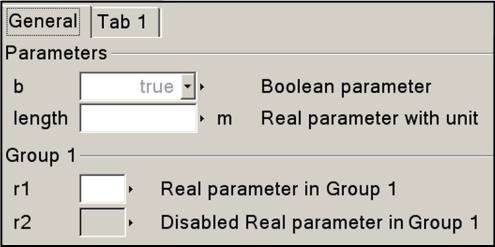
\includegraphics[scale=0.5]{disabledparameter}
\quad
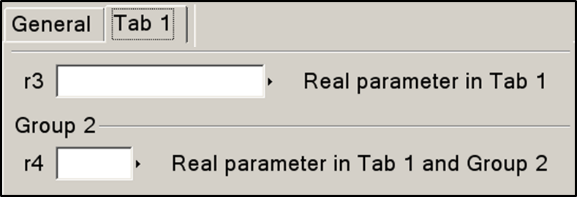
\includegraphics[scale=0.5]{tabparameter}\\
\end{center}
\end{example}

\subsection{Connector Sizing}\label{connector-sizing}

This section describes the \lstinline!connectorSizing! annotation inside a \lstinline!Dialog! annotation.
The value of \lstinline!connectorSizing! must be a literal \lstinline!false! or \lstinline!true!.
If \lstinline!connectorSizing = false!, this annotation has no effect.
If \lstinline!connectorSizing = true!, the corresponding variable must be declared with the \lstinline!parameter! prefix, must be a subtype of a scalar \lstinline!Integer! and must have a literal default value of zero.

\begin{nonnormative}
The reason why \lstinline!connectorSizing! must be given a literal value is that if the value is an expression,
the \lstinline!connectorSizing! functionality is conditional and this will then lead easily to wrong models.

The default value of the variable must be zero since this annotation
is designed for a parameter that is used as vector dimension, and the
dimension of the vector should be zero when the component is dragged or
redeclared.  Furthermore, when a tool does not support the
\lstinline!connectorSizing! annotation, dragging will still result in a correct
model.
\end{nonnormative}

If \lstinline!connectorSizing = true!, a tool may set the parameter value in a modifier automatically, if used as dimension size of a vector of connectors.
In that case the parameter should not be modified by the user, and a tool may choose to not display that parameter in the dialog or display it with disabled input field.

\begin{nonnormative}
The \lstinline!connectorSizing! annotation is used in cases
where connections to a vector of connectors shall be made and a new
connection requires to resize the vector and to connect to the new index
(unary connections). The annotation allows a tool to perform these two
actions in many cases automatically. This is, e.g., very useful for
state machines and for certain components of fluid libraries.
\end{nonnormative}

\begin{nonnormative}
The following part is non-normative text and describes a useful
way to handle the \lstinline!connectorSizing! annotation in a tool (still a tool may
use another strategy and/or may handle other cases than described
below).
The recommended rules are clarified at hand of the following
example which represents a connector and a model from the
\lstinline!Modelica.StateGraph! library (note that they may be modified or renamed in future versions):
\begin{lstlisting}[language=modelica]
connector Step_in // Only 1:1 connections are possible since input used
  output Boolean occupied;
  input Boolean set;
end Step_in;

block Step
  // nIn cannot be set through the dialog (but maybe shown)
  parameter Integer nIn=0 annotation(Dialog(connectorSizing=true));
  Step_in inPorts[nIn];
  $\ldots$
end Step;
\end{lstlisting}
If the parameter is used as dimension size of a vector of
connectors, it is automatically updated according to the following
rules:
\begin{enumerate}
\item \label{connectorSizing:addVector}
  If a new connection line is drawn between one outside and one
  inside vector of connectors both dimensioned with (\lstinline!connectorSizing!)
  parameters, a connection between the two vectors is performed and the
  (\lstinline!connectorSizing!) parameter is propagated from connector to component.
  Other types of outside connections do not lead to an automatic update
  of a (\lstinline!connectorSizing!) parameter. \emph{Example:} Assume there is a
  connector \lstinline!inPorts! and a component \lstinline!step1!:
\begin{lstlisting}[language=modelica]
parameter Integer nIn=0 annotation(Dialog(connectorSizing=true));
Step_in inPorts[nIn];
Step step1(nIn=0);
\end{lstlisting}
  Drawing a connection line between connectors \lstinline!inPorts! and
  \lstinline!step1.inPorts! results in:
\begin{lstlisting}[language=modelica]
  parameter Integer nIn=0 annotation(Dialog(connectorSizing=true));
  Step_in inPorts[nIn];
  Step step1(nIn=nIn); // nIn=0 changed to nIn=nIn
equation
  connect(inPorts, step1.inPorts); // new connect-equation
\end{lstlisting}
\item\label{connectorSizing:deleteVector}
  If a connection line is deleted between one outside and one inside vector of connectors both dimensioned with (\lstinline!connectorSizing!) parameters, the \lstinline!connect!-equation is removed and the (\lstinline!connectorSizing!) parameter of the component is set to zero or the modifier is removed.
  \emph{Example:} Assume the connection line in the resulting example in case~\ref{connectorSizing:addVector} is removed.
  This results in:
\begin{lstlisting}[language=modelica]
parameter Integer nIn=0 annotation(Dialog(connectorSizing=true));
Step_in inPorts[nIn];
Step step1; // modifier nIn=nIn is removed
\end{lstlisting}
\item \label{connectorSizing:addScalar}
  If a new connection line is drawn to an inside connector with
  \lstinline!connectorSizing! and case~\ref{connectorSizing:addVector} does not apply then, the parameter is
  incremented by one and the connection is performed for the new highest
  index. \emph{Example:} Assume that 3 connections are present and a new
  connection is performed. The result is:
\begin{lstlisting}[language=modelica]
  Step step1(nIn=4); // index changed from nIn=3 to nIn=4
equation
  connect($\ldots$, step1.inPorts[4]); // new connect-equation
\end{lstlisting}
  In some applications, like state machines, the vector index is
  used as a priority, e.g., to define which transition is firing if
  several transitions become active at the same time instant. It is then
  not sufficient to only provide a mechanism to always connect to the
  last index. Instead, some mechanism to select an index conveniently
  should be provided.
\item \label{connectorSizing:deleteScalar}
  If a connection line is deleted to an inside connector with
  \lstinline!connectorSizing! and case~\ref{connectorSizing:deleteVector} does not apply then, then the
  (\lstinline!connectorSizing!) parameter is decremented by one and all connections
  with index above the deleted connection index are also decremented by
  one. \emph{Example:}Assume there are 4 connections:
\begin{lstlisting}[language=modelica]
  Step step1(nIn=4);
equation
  connect(a1, step1.inPorts[1]);
  connect(a2, step1.inPorts[2]);
  connect(a3, step1.inPorts[3]);
  connect(a4, step1.inPorts[4]);
\end{lstlisting}
  and the connection from \lstinline!a2! to \lstinline!step1!. \lstinline!inPorts[2]! is deleted.
  This results in
\begin{lstlisting}[language=modelica]
  Step step1(nIn=3);
equation
  connect(a1, step1.inPorts[1]);
  connect(a3, step1.inPorts[2]);
  connect(a4, step1.inPorts[3]);
\end{lstlisting}
\end{enumerate}

These rules also apply if the connectors and/or components are defined in superclass.

\emph{Example:} Assume that \lstinline!step1! is defined in superclass \lstinline!MyCompositeStep! with 3 connections, and a new connection is performed in a derived class.
The result is:
\begin{lstlisting}[language=modelica]
  extends MyCompositeStep(step1(nIn=4)); // new modifier nIn=4
equation
  connect($\ldots$, step1.inPorts[4]);  // new connect-equation
\end{lstlisting}
\end{nonnormative}

\section{Annotations for Version Handling}\label{annotations-for-version-handling}

A top-level package or model can specify the version of top-level
classes it uses, its own version number, and if possible how to convert
from previous versions. This can be used by a tool to guarantee that
consistent versions are used, and if possible to upgrade usage from an
earlier version to a current one.

\subsection{Version Numbering}\label{version-numbering}

Version numbers are of the forms:
\begin{itemize}
\item
  Main release versions: \lstinline[language=grammar]!""" UNSIGNED-INTEGER { "." UNSIGNED-INTEGER } """!\\
  Example: \lstinline!"2.1"!
\item
  Pre-release versions: \lstinline[language=grammar]!""" UNSIGNED-INTEGER { "." UNSIGNED-INTEGER } " " {S-CHAR} """!\\
  Example: \lstinline!"2.1 Beta 1"!
\item
  Un-ordered versions: \lstinline[language=grammar]!""" NON-DIGIT {S-CHAR} """!\\
  Example: \lstinline!"Test 1"!
\end{itemize}

The main release versions are ordered using the hierarchical numerical
names, and follow the corresponding pre-release versions. The
pre-release versions of the same main release version are internally
ordered alphabetically.

\subsection{Version Handling}\label{version-handling}

In a top-level class, the version number and the dependency to earlier versions of this class are defined using one or more of the following annotations:
% TODO: Syntax below is a mess: neither Modelica, pseudo-code record, nor grammar.
\begin{itemize}
\item
  \lstinline!version = CURRENT-VERSION-NUMBER!\annotationindex{version}\\
  Defines the version number of the model or package.
  All classes within this top-level class have this version number.
\item
  \lstinline!conversion(noneFromVersion = VERSION-NUMBER)!\annotationindex{conversion}\\
  Defines that user models using the \lstinline!VERSION-NUMBER! can be upgraded to the \lstinline!CURRENT-VERSION-NUMBER! of the current class without any changes.
\item
  \lstinline!conversion(from(version = Versions, [to=VERSION-NUMBER,] Convert))!\\
  where \emph{Versions} is \lstinline!VERSION-NUMBER! \textbar{} \lstinline!{VERSION-NUMBER, VERSION-NUMBER, $\ldots$}! and \lstinline!Convert! is \lstinline!script="$\ldots$"! \textbar{} \lstinline!change={conversionRule(), $\ldots$, conversionRule()}!\\*[.5ex]
  Defines that user models using the \lstinline!VERSION-NUMBER! or any of the given \lstinline!VERSION-NUMBER! can be upgraded to the given \lstinline!VERSION-NUMBER! (if the to-tag is missing this is the \lstinline!CURRENT-VERSION-NUMBER!) of the current class by applying the given conversion rules.
  The script consists of an unordered sequence of \lstinline!conversionRule();! (and optionally Modelica comments).
  The \lstinline!conversionRule! functions are defined in \cref{conversion-rules}.

  \begin{nonnormative}
  The to-tag is added for clarity and optionally allows a tool to convert in multiple steps.
  \end{nonnormative}
\item
  \lstinline!uses(IDENT (version = VERSION-NUMBER [, versionBuild=INTEGER] [, dateModified=STRING] ) )!\annotationindex{uses}\\
  Defines that classes within this top-level class uses version \lstinline!VERSION-NUMBER! of classes within the top-level class \lstinline!IDENT!.
\end{itemize}

The annotations \lstinline!uses! and \lstinline!conversion! may contain several different sub-entries.

\begin{example}
\begin{lstlisting}[language=modelica]
package Modelica
  $\ldots$
  annotation(version="3.1",
  conversion(noneFromVersion="3.1 Beta 1",
  noneFromVersion="3.1 Beta 2",
  from(version={"2.1", "2.2", "2.2.1"},
  script="convertTo3.mos"),
  from(version="1.5",
  script="convertFromModelica1_5.mos")));
end Modelica;

model A
  $\ldots$
  annotation(version="1.0",
  uses(Modelica(version="1.5")));
end A;

model B
  $\ldots$
  annotation(uses(Modelica(version="3.1 Beta 1")));
end B;
\end{lstlisting}
In this example the model \lstinline!A! uses an older version of the
Modelica library and can be upgraded using the given script, and model
\lstinline!B! uses an older version of the Modelica library but no changes are
required when upgrading.
\end{example}

\subsubsection{Conversion rules}\label{conversion-rules}

% Using mbox to avoid having line starting with ","
There are a number of functions: \lstinline!convertClass!, \lstinline!convertClassIf!,
\lstinline!convertElement!, \mbox{\lstinline!convertModifiers!,} \lstinline!convertMessage! defined as follows. The
calls of these functions do not directly convert, instead they define
conversion rules as below.
It is recommended, but not required, to terminate each such function call with a semi-colon.
The order between the function calls does not matter, instead the longer paths (in terms of number of hierarchical names)
are used first as indicated below, and it is an error if there are any
ambiguities.

The conversion should generate correct Modelica models using the new version of the library
corresponding to the old version.

\begin{nonnormative}
Whenever possible tools should preserve the original style of the model, e.g.\ use of imports.
\end{nonnormative}

These functions can be called with literal strings or array of strings
and vectorize according to \cref{scalar-functions-applied-to-array-arguments}.

All of these convert-functions only use inheritance among user models, and not in the library that is used for the conversion -- thus conversions of base classes will require multiple conversion calls; this ensures that the conversion is independent of the new library structure.
The name of the class used as argument to \lstinline!convertElement! and \lstinline!convertModifiers! is similarly the old name of the class, i.e.\ the name before it is possibly converted by \lstinline!convertClass!.

\begin{nonnormative}
Specifying conversions using the old name of a class allows the conversion to be done without access to the old
version of the library (by suitable modifications of the lookup).  Another alternative is to use the old version
of the library during the conversion.
\end{nonnormative}

\paragraph*{convertClass("OldClass", "NewClass")}\label{convertclassoldclassnewclass}\annotationindex{convertClass}

Convert class \lstinline!OldClass! to \lstinline!NewClass!.

Match longer path first, so if converting both \lstinline!A! to \lstinline!C! and \lstinline!A.B! to \lstinline!D! then \lstinline!A.F! is converted to \lstinline!C.F! and \lstinline!A.B.E! to \lstinline!D.E!. This is considered before \lstinline!convertMessage! for the same \lstinline!OldClass!.

\begin{example}
Consider the following as part of a conversion script:
\begin{lstlisting}[language=modelica]
convertClass("Modelica.SIunits", "Modelica.Units.SI");
convertClass("Modelica.SIunits.Icons", "Modelica.Units.Icons");
\end{lstlisting}
This ensures that for example \lstinline!Modelica.SIunits.Length! is converted to \lstinline!Modelica.Units.SI.Length!
and \lstinline!Modelica.SIunits.Icons! is converted to \lstinline!Modelica.SIunits.Icons!.
\end{example}

\paragraph*{convertClassIf("OldClass", "oldElement", "whenValue", "NewClass")}\label{convertclassifoldclass-oldelement-whenvalue-newclass}\annotationindex{convertClassIf}

Convert class \lstinline!OldClass! to \lstinline!NewClass! if the literal modifier for
\lstinline!oldElement! has the value \lstinline!whenValue!, and also remove the modifier for
\lstinline!oldElement!.

These are considered before \lstinline!convertClass! and \lstinline!convertMessage! for the same \lstinline!OldClass!.

The old element should be of a \lstinline!Boolean!, \lstinline!Integer!, \lstinline!String!, or enumeration
type and the match is based on the literal value of the modifier.
For string elements the value argument to \lstinline!convertClassIf! shall be up-quoted, e.g.\ \lstinline!"\"My String\""!,
and for enumeration literals only the enumeration literal part of the old value matters, e.g., \lstinline!red!
for \lstinline!"Colors.red"!.

\paragraph*{convertElement("OldClass", "OldName", "NewName")}\label{convertelementoldclassoldnamenewname}\annotationindex{convertElement}

In \lstinline!OldClass!, convert element \lstinline!OldName! to \lstinline!NewName!.  Both \lstinline!OldName! and \lstinline!NewName! normally refer to components, but they may also refer to
class-parameters, or hierarchical names.  For hierarchical names, the longest match is used first.

For replaceable classes in packages (and replaceable classes in other classes) \lstinline!convertElement! shall
be used if the class is renamed within the package (or class), whereas \lstinline!convertClass! shall only be used if the class
is placed outside of the package (or class).

\begin{nonnormative}
The latter case indicates a problem with overuse of replaceable classes in the previous design of the library.
\end{nonnormative}

\begin{example}
Consider the following as part of a conversion script:
\begin{lstlisting}[language=modelica]
convertElement({"Modelica.Mechanics.MultiBody.World",
                "Modelica.Mechanics.MultiBody.World.gravityAcceleration"},
                "mue", "mu");
\end{lstlisting}
This implies that
\begin{lstlisting}[language=modelica]
Modelica.Mechanics.MultiBody.World world(mue=2);
function f=Modelica.Mechanics.MultiBody.World.gravityAcceleration(mue=4);
\end{lstlisting}
is converted to:
\begin{lstlisting}[language=modelica]
Modelica.Mechanics.MultiBody.World world(mu=2);
function f=Modelica.Mechanics.MultiBody.World.gravityAcceleration(mu=4);
\end{lstlisting}
\end{example}

\paragraph*{convertModifiers}\label{convertmodifiers}\annotationindex{convertModifiers}
\ % Dummy paragraph content to ensure listing below starts on a fresh line.

\begin{lstlisting}[language=modelica]
convertModifiers("OldClass",
  {"OldModifier1=default1", "OldModifier2=default2", $\ldots$},
  {"NewModifier1=$\ldots$%OldModifier2%$\ldots$", "NewModifier2=$\ldots$", $\ldots$}
  [, simplify=true]);
\end{lstlisting}

Normal case; if any modifier among \lstinline!OldModifier! exist then replace all of them with the list of\linebreak[4] \lstinline!NewModifiers!.
The \lstinline!$\ldots$%OldModifier2%$\ldots$! indicate an expression that may involve the values of the old modifiers (tools are responsible for adding parenthesis if needed).
The lists of old and new modifiers can have different lengths.
The defaults (if present) are used if there are multiple \lstinline!OldModifier! and not all are set in the component instance.
The defaults are optional if there is at most one \lstinline!OldModifier! element, and should otherwise be provided.

If \lstinline!simplify! is specified and true then perform obvious simplifications
to clean up the new modifier; otherwise leave as is.

\begin{nonnormative}
Note: \lstinline!simplify! is primarily intended for converting enumerations and emulated enumerations that naturally lead to large nested \lstinline!if!-expressions.
The simplifications may also simplify parts of the original expression.
\end{nonnormative}

If the modifiers contain literal string values they must be quoted.

Behaviour in unusual cases:
\begin{itemize}
\item
  if \lstinline!NewModifier! list is empty then the modifier is just removed
\item
  If \lstinline!OldModifer! list is empty it is added for all uses of the class
\item
  If \lstinline!OldModifier$i$! is \lstinline!cardinality(a) = 0! the conversion will only be applied for a component comp if there are no inside connections to \lstinline!comp.a!. This can be combined with other modifiers that are handled in the usual way.
\item
  If \lstinline!OldModifier$i$! is \lstinline!cardinality(a) = 1! the conversion will only be applied for a component comp if there are any inside connections to \lstinline!comp.a!.
\end{itemize}

The converted modifiers and existing modifiers are merged such that the existing modifiers take precedence over the result of \lstinline!convertModifiers!.
A diagnostics is recommended if this merging removes some modifiers unless those modifiers are identical or it is the special case of an empty \lstinline!OldModifier! list.
\begin{nonnormative}
This can be used to handle the case where the default value was changed.
\end{nonnormative}

Converting modifiers with cardinality is used to remove the deprecated operator \lstinline!cardinality! from model libraries, and replace tests on cardinality in models by parameters explicitly enabling the different cases.
The case where the old class is used as a base class, and there exist outside connections to \lstinline!a!, and there is \lstinline!convertModifiers! involving the cardinality of \lstinline!a! is not handled.

\begin{nonnormative}
Having a parameter for explicitly enabling the different cases means that instead of model \lstinline!A! internally testing if its
connector \lstinline!B! is connected, there will be a parameter for enabling connector \lstinline!B!, and the conversion ensures that
each component of model \lstinline!A! will have this parameter set accordingly.

In case a parameter is simply renamed it is preferable to use \lstinline!convertElement!, since that also handles e.g.\ binding equations
using the parameter.
\end{nonnormative}


\begin{example}
The conversion
\begin{lstlisting}[language=modelica]
convertClass("Modelica.Thermal.FluidHeatFlow.Components.IsolatedPipe",
             "Modelica.Thermal.FluidHeatFlow.Components.Pipe");
convertModifiers({"Modelica.Thermal.FluidHeatFlow.Components.IsolatedPipe"},
   fill("",0), {"useHeatPort=false"});

convertClass("Modelica.StateGraph.Temporary.NumericValue",
             "Modelica.Blocks.Interaction.Show.RealValue");
convertModifiers("Modelica.StateGraph.Temporary.NumericValue",
   {"Value"}, {"number=%Value%"});
convertModifiers("Modelica.StateGraph.Temporary.NumericValue",
   {"hideConnector"}, {"use_numberPort=not %hideConnector%"});

convertModifiers("Modelica.Blocks.Math.LinearDependency",
   {"y0=0", "k1=0", "k2=0"}, {"y0=%y0%", "k1=%y0%*%k1%", "k2=%y0%*%k2%"},
   true);
convertClass(
   "Modelica.Electrical.Machines.BasicMachines.QuasiStationaryDCMachines",
   "Modelica.Electrical.Machines.BasicMachines.QuasiStaticDCMachines");
convertElement("Modelica.Electrical.Machines.Interfaces.PartialBasicDCMachine",
                "quasiStationary", "quasiStatic");
convertElement("Modelica.Electrical.Machines.BasicMachines.QuasiStationaryDCMachines.DC_ElectricalExcited",
                "quasiStationary", "quasiStatic");
\end{lstlisting}
converts
\begin{lstlisting}[language=modelica]
Modelica.Thermal.FluidHeatFlow.Components.IsolatedPipe pipe1;
Modelica.StateGraph.Temporary.NumericValue tempValue(Value=10,
   hideConnector=true);
Modelica.Blocks.Math.LinearDependency linearDep(y0=2, k2=1);
model A
  import Modelica.Electrical.Machines.BasicMachines;
  extends BasicMachines.QuasiStationaryDCMachines.DC_ElectricalExcited;
end A;
model B
  extends A;
  Boolean b=quasiStationary;
end B;
\end{lstlisting}
to
\begin{lstlisting}[language=modelica]
Modelica.Thermal.FluidHeatFlow.Components.Pipe pipe1(useHeatPort=false);
Modelica.Blocks.Interaction.Show.RealValue(number=10, use_numberPort=not true);
Modelica.Blocks.Math.LinearDependency linearDep(y0=2, k1=0, k2=2);
model A
  import Modelica.Electrical.Machines.BasicMachines;
  extends BasicMachines.QuasiStaticDCMachines.DC_ElectricalExcited;
end A;
model B
  extends A;
  Boolean b=a.quasiStatic;
end B;
\end{lstlisting}
The \lstinline!convertElement! call for \lstinline!DC_ElectricalExcited! is needed to avoid relying on base classes in the original library where \lstinline!DC_ElectricalExcited! inherits from \lstinline!PartialBasicDCMachine!.
However, the inheritance among the models to convert (in this case \lstinline!B! inherits from \lstinline!A!) should be handled.
\end{example}

\paragraph*{convertMessage("OldClass", "Failed Message")}\label{convertmessageoldclass-failed-message}\annotationindex{convertMessage}

For any use of \lstinline!OldClass! (or element of \lstinline!OldClass!) report that conversion
could not be applied with the given message.

\begin{nonnormative}
This may be useful if there is no possibility to convert a specific class. An alternative is to construct \lstinline!ObsoleteLibraryA! for problematic
cases, which may be more work but allows users to directly run the models after the conversion and later convert them.
\end{nonnormative}

\paragraph*{convertMessage("OldClass", "Failed Message", "oldElement")}\label{convertmessageoldclass-failed-message2}

For any use of \lstinline!oldElement! in \lstinline!OldClass! report that conversion
could not be applied with the given message.

\begin{nonnormative}
This is useful if there is no possibility to convert a specific parameter (or other element), especially if it rarely modified.  If the parameter had no impact on the model it can be removed using \lstinline!convertModifiers!, see \cref{convertmodifiers}.
\end{nonnormative}

\subsection{Mapping of Versions to File System}\label{mapping-of-versions-to-file-system}

A top-level class, \lstinline!IDENT!, with version \lstinline!VERSION-NUMBER! can be stored in
one of the following ways in a directory given in the \lstinline!MODELICAPATH!:
\begin{itemize}
\item
  The file \lstinline!IDENT ".mo"!\\
  Example: \filename{Modelica.mo}
\item
  The file \lstinline!IDENT " " VERSION-NUMBER ".mo"!\\
  Example: \filename{Modelica 2.1.mo}
\item
  The directory \lstinline!IDENT! with the file \filename{package.mo} directly inside it\\
  Example: \filename{Modelica/package.mo}
\item
  The directory \lstinline!IDENT " " VERSION-NUMBER! with the file \filename{package.mo} directly inside it\\
  Example: \filename{Modelica 2.1/package.mo}
\end{itemize}

This allows a tool to access multiple versions of the same package.

\subsection{Version Date and Build Information}\label{version-date-and-build-information}

Besides version information, a top-level class can have additionally the following top-level annotations to specify associated information to the version number:%
\begin{lstlisting}[language=modelica]
String versionDate   "UTC date of first version build (in format: YYYY-MM-DD)";
Integer versionBuild "Larger number is a more recent maintenance update";
String dateModified  "UTC date and time of the latest change to the package
                      in the following format (with one space between date
                      and time): YYYY-MM-DD hh:mm:ssZ";
String revisionId    "Revision identifier of the version management system used
                      to manage this library. It marks the latest submitted
                      change to any file belonging to the package";
\end{lstlisting}%
\annotationindex{versionDate}\annotationindex{versionBuild}\annotationindex{dateModified}\annotationindex{revisionId}

\begin{example}
\begin{lstlisting}[language=modelica,mathescape=false]
package Modelica
  $\ldots$
  annotation(version = "3.0.1",
  versionDate = "2008-04-10",
  versionBuild = 4,
  dateModified = "2009-02-15 16:33:14Z",
  revisionId = "$Id:: package.mo 2566 2009-05-26 13:25:54Z #$");
end Modelica;

model M1
  annotation(uses(Modelica(version = "3.0.1"))); // Common case
end M1

model M2
  annotation(uses(Modelica(version = "3.0.1", versionBuild = 4)));
end M2
\end{lstlisting}
\end{example}

The meanings of these annotations are:
\begin{itemize}
\item
  \lstinline!version! is the version number of the released library,
  see \cref{version-handling}.
\item
  \lstinline!versionDate! is the date in UTC format (according to ISO
  8601) when the library was released. This string is updated by the
  library author to correspond with the version number.
\item
  \lstinline!versionBuild! is the optional build number of the library.
  When a new version is released \lstinline!versionBuild! should be omitted or
  \lstinline!versionBuild = 1!. There might be bug fixes to the library that do
  not justify a new library version. Such maintenance changes are called
  a \emph{build} release of the library. For every new maintenance change,
  the \lstinline!versionBuild! number is increased. A \lstinline!versionBuild! number $A$
  that is higher than \lstinline!versionBuild! number $B$, is a newer release of the
  library. There are no conversions between the same versions with
  different build numbers.

  Two releases of a library with the same \lstinline!version! but different \lstinline!versionBuild! are in general assumed to be compatible.
  In special cases, the \lstinline!uses!-clause of a model may specify \lstinline!versionBuild! and/or \lstinline!dateModified!.
  In such a case the tool is expected to give a warning if there is a mismatch between library and model.
\item
  \lstinline!dateModified! is the UTC date and time (according to ISO
  8601) of the last modification of the package.

  \begin{nonnormative}
  The intention is that a Modelica tool updates this annotation whenever the package or part of it was modified and is saved on
  persistent storage (like file or database system).
  \end{nonnormative}
\item
  \lstinline!revisionId! is a tool specific revision identifier
  possibly generated by a source code management system (e.g.\ Subversion
  or CVS). This information exactly identifies the library
  source code in the source code management system.
\end{itemize}

The \lstinline!versionBuild! and \lstinline!dateModified! annotations can also be specified in
the \lstinline!uses! annotation (together with the version number).

\begin{nonnormative}
It is recommended that tools do not automatically store \lstinline!versionBuild! and \lstinline!dateModified! in the \lstinline!uses! annotation.
\end{nonnormative}

\section{Annotations for Access Control to Protect Intellectual Property}\label{annotations-for-access-control-to-protect-intellectual-property}

This section presents annotations to define the protection and the
licensing of packages. The goal is to unify basic mechanisms to control
the access to a package in order to protect the intellectual property
contained in it. This information is used to encrypt a package and bind
it optionally to a particular target machine, and/or restrict the usage
for a particular period of time.

\begin{nonnormative}
Protecting the intellectual property of a Modelica package is
considerably more difficult than protecting code from a programming
language. The reason is that a Modelica tool needs the model equations
in order that it can process the equations symbolically, as needed for
acausal modeling. Furthermore, if a Modelica tool generates C-code of
the processed equations, this code is then potentially available for
inspection by the user. Finally, the Modelica tool vendors have to be
trusted, that they do not have a backdoor in their tools to store the
(internally) decrypted classes in human readable format. The only way to
protect against such misuse is legally binding warranties of the tool
vendors.

The intent of this section is to enable a library vendor to
maintain one source version of their Modelica library that can be
encrypted and used with several different Modelica tools, using
different encryption formats.
\end{nonnormative}

The following definitions relate to access control.

\begin{definition}[Protection]\index{protection!access control}
Define what parts of a class are visible.
\end{definition}

\begin{definition}[Obfuscation]\index{obfuscation!access control}
Changing a Modelica class or generated code so that it is difficult to inspect by a user (e.g.\ by automatically renaming variables to non-meaningful names).
\end{definition}

\begin{definition}[Encryption]\index{encryption!access control}
Encoding of a model or a package in a form so that the modeler cannot inspect any content of a class without an appropriate key.  An encrypted package that has the \lstinline!Protection! annotation
is read-only; the way to modify it is to generate a new encrypted version.
\end{definition}

\begin{definition}[Licensing]\index{licensing!access control}
Restrict the use of an encrypted package for particular users for a specified period of time.
\end{definition}

In this section annotations are defined for protection and licensing.  Obfuscation and encryption are not standardized.

Protection and licensing are both defined inside the \fmtannotationindex{Protection} annotation:
\begin{lstlisting}[language=modelica]
annotation(Protection($\ldots$));
\end{lstlisting}

\subsection{Protection of Classes}\label{protection-of-classes}

A class may have the following annotations to define what parts of a class are visible, and only the parts explicitly listed as visible below can be accessed (if a class is encrypted and no \lstinline!Protection! annotation is defined, the access annotation has the default value \lstinline!Access.documentation!):
\begin{lstlisting}[language=modelica]
type Access =
  enumeration(hide, icon, documentation, diagram,
              nonPackageText, nonPackageDuplicate,
              packageText, packageDuplicate);
annotation(Protection(access = Access.documentation));
\end{lstlisting}

The items of the \fmtannotationindex{Access} enumeration have the following meanings:
\begin{enumerate}
\item
  \lstinline!Access.hide!\\
  Do not show the class anywhere (it is not possible to inspect any part
  of the class).
\item
  \lstinline!Access.icon!\\
  The class can be instantiated and public parameter, constant, input, output variables as well as public connectors can be accessed, as well as the \lstinline!Icon! annotation, as defined in \cref{annotations-for-graphical-objects} (the declared information of these elements can be shown).  Additionally, the class name and its description text can be accessed.
\item
  \lstinline!Access.documentation!\\
  Same as \lstinline!Access.icon! and additionally the \lstinline!Documentation! annotation (as defined in \cref{annotations-for-documentation}) can be accessed.  HTML-generation in the \lstinline!Documentation! annotation is normally performed before encryption, but the generated HTML is intended to be used with the encrypted package.  Thus the HTML-generation should use the same access as the encrypted version -- even before encryption.
\item
  \lstinline!Access.diagram!\\
  Same as \lstinline!Access.documentation! and additionally, the \lstinline!Diagram! annotation, and all components and \lstinline!connect!-equations that have a graphical annotation can be accessed.
\item
  \lstinline!Access.nonPackageText!\\
  Same as \lstinline!Access.diagram! and additionally if it is not a package: the whole class definition can be accessed (but that text cannot be copied, i.e., you can see but not copy the source code).
\item
  \lstinline!Access.nonPackageDuplicate!\\
  Same as \lstinline!Access.nonPackageText! and additionally if it is not a package: the class, or part of the class, can be copied.
\item
  \lstinline!Access.packageText!\\
  Same as \lstinline!Access.diagram! (note: \emph{not} including all rights of \lstinline!Access.nonPackageDuplicate!) and additionally the whole class definition can be accessed (but that text cannot be copied, i.e., you can see but not copy the source code).
\item
  \lstinline!Access.packageDuplicate!\\
  Same as \lstinline!Access.packageText! and additionally the class, or part of the class, can be copied.
\end{enumerate}

The \lstinline!access! annotation holds for the respective class and all classes
that are hierarchically on a lower level, unless overridden by a
\lstinline!Protection! annotation with \lstinline!access!.
Overriding \lstinline!access=Access.hide! or \lstinline!access=Access.packageDuplicate!
has no effect.

\begin{example}
If the annotation is given on the top level of a package and at no other class in this package, then the \lstinline!access! annotation holds for all classes in this package.
\end{example}

\begin{nonnormative}
It is currently not standardized which result variables are
accessible for plotting. It seems natural to not introduce new flags for
this, but reuse the \lstinline!Access.XXX! definition, e.g., for \lstinline!Access.icon!
only the variables can be stored in a result file that can also be
inspected in the class, and for \lstinline!Access.nonPackageText! all public
and protected variables can be stored in a result file, because all
variables can be inspected in the class.

\begin{lstlisting}[language=modelica]
package CommercialFluid // Access icon, documentation, diagram
  package Examples // Access icon, documentation, diagram
    model PipeExample // Access everything, can be copied
    end PipeExample;

    package Circuits // Access icon, documentation, diagram
      model ClosedCircuit // Access everything, can be copied
      end ClosedCircuit;
    end Circuits;

    model SecretExample // No access
      annotation(Protection(access=Access.hide));
    end SecretExample;
    annotation(Protection(access=Access.nonPackageDuplicate));
  end Examples;

  package Pipe // Access icon
    model StraightPipe // Access icon
    end StraightPipe;
    annotation(Protection(access=Access.icon));
  end Pipe;

  package Vessels // Access icon, documentation, diagram
    model Tank // Access icon, documentation, diagram, text
    end Tank;
  end Vessels;
  annotation(Protection(access=Access.nonPackageText));
end CommercialFluid;
\end{lstlisting}
\end{nonnormative}

\subsection{Licensing}\label{licensing}

In this section annotations within the \lstinline!Protection! annotation are
defined to restrict the usage of the encrypted package:
\begin{lstlisting}[language=modelica]
record Protection
  $\ldots$
  String features[:] = fill("", 0) "Required license features";
  record License
    String libraryKey;
    String licenseFile = "" "Optional, default mapping if empty";
  end License;
end Protection;
\end{lstlisting}
The \fmtannotationindex{License} annotation has only an effect on the top of an encrypted class and is then valid for the whole class hierarchy.
(Usually the licensed class is a package.)
The \lstinline!libraryKey! is a secret string from the library vendor and is the protection mechanism so that a user cannot generate his/her own authorization file since the \lstinline!libraryKey! is unknown to him/her.

The \lstinline!features! annotation defines the required license options. If the
features vector has more than one element, then at least a license
feature according to one of the elements must be present. As with the
other annotations, the \lstinline!features! annotation holds for the respective
class and for all classes that are hierarchically on a lower level,
unless further restricted by a corresponding annotation. If no license
according to the \lstinline!features! annotation is provided in the
authorization file, the corresponding classes are not visible and cannot
be used, not even internally in the package.

\begin{example}
\begin{lstlisting}[language=modelica]
// Requires license feature "LicenseOption"
annotation(Protection(features={"LicenseOption"}));

// Requires license features "LicenseOption1" or "LicenseOption2"
annotation(Protection(features={"LicenseOption1", "LicenseOption2"}));

// Requires license features ("LicenseOption1" and "LicenseOption2") or "LicenseOption3"
annotation(Protection(features={"LicenseOption1 LicenseOption2", "LicenseOption3"}));
\end{lstlisting}
\end{example}

In order that the protected class can be used either a tool specific license manager, or a license file (called \lstinline!licenseFile!) must be present.
The license file is standardized.
It is a Modelica package without classes that has a \lstinline!Protection! annotation of the following form which specifies a sequence of target records, which makes it natural to define start/end dates for different sets of targets individually:
\begin{lstlisting}[language=modelica]
record Authorization
  String licensor = "" "Optional string to show information about the licensor";
  String libraryKey "Matching the key in the class. Must be encrypted and not visible";
  License license[:] "Definition of the license options and of the access rights";
end Authorization;

record License
  String licensee = "" "Optional string to show information about the licensee";
  String id[:] "Unique machine identifications, e.g.\ MAC addresses";
  String features[:] = fill("", 0) "Activated library license features";
  String startDate = "" "Optional start date in UTCformat YYYY-MM-DD";
  String expirationDate = "" "Optional expiration date in UTCformat YYYY-MM-DD";
  String operations[:] = fill("", 0) "Library usage conditions";
end License;
\end{lstlisting}%
\index{Authorization@\robustinline{Authorization}!license file}\index{License@\robustinline{License}!license file}

The format of the strings used for \lstinline!libraryKey! and \lstinline!id! are not specified
(they are vendor specific). The \lstinline!libraryKey! is a secret of the library
developer. The \lstinline!operations! define the usage conditions and the following
are default names:
\begin{itemize}
\item
  \lstinline!"ExportBinary"! Binary code generated from the Modelica code of the
  library can be included in binaries produced by a simulation
  tool.
\item
  \lstinline!"ExportSource"! Source code generated from the Modelica code of the
  library can be included in sources produced by a simulation tool.
\end{itemize}

Additional tool-specific names can also be used. To protect the
\lstinline!libraryKey! and the target definitions, the authorization file must
be encrypted and must never show the \lstinline!libraryKey!.

\begin{nonnormative}
All other information, especially licensor and license should be visible, in order
that the user can get information about the license. It is useful to
include the name of the tool in the authorization file name with which
it was encrypted. Note, it is not useful to store this information in
the annotation, because only the tool that encrypted the \lstinline!Authorization!
package can also decrypt it.
\end{nonnormative}

\begin{example}
(Before encryption:)
\begin{lstlisting}[language=modelica]
// File MyLibrary\package.mo
package MyLibrary
  annotation(Protection(License(libraryKey="15783-A39323-498222-444ckk4ll",
  licenseFile="MyLibraryAuthorization_Tool.mo_lic), $\ldots$));
end MyLibrary;

// File MyLibrary\MyLibraryAuthorization_Tool.mo\
// (authorization file before encryption)
package MyLibraryAuthorization_Tool
  annotation(Authorization(
  libraryKey="15783-A39323-498222-444ckk4ll",
  licensor ="Organization A\nRoad, Country",
 license={
  License(licensee="Organization B, Mr.X",
    id ={"lic:1269"}), // tool license number
  License(licensee="Organization C, Mr. Y",
    id ={"lic:511"}, expirationDate="2010-06-30",
   operations={"ExportBinary"}),
  License(licensee="Organization D, Mr. Z",
    id ={"mac:0019d2c9bfe7"}) // MAC address
  }));
end MyLibraryAuthorization_Tool;
\end{lstlisting}
\end{example}


\section{Annotations for Functions}\label{annotations-for-functions}

See \crefnameref{derivatives-and-inverses-of-functions}, \crefnameref{function-inlining-and-event-generation}, and \crefnameref{annotations-for-external-libraries-and-include-files}.


\section{Annotation Choices for Modifications and Redeclarations}\label{annotation-choices-for-modifications-and-redeclarations}

See \crefnameref{annotation-choices-for-suggested-redeclarations-and-modifications}.


% Unit Expressions
\chapter{Unit Expressions}\doublelabel{unit-expressions}

Unless otherwise stated, the syntax and semantics of unit expressions in
Modelica are conform with the international standards ISO 31/0-1992
"General principles concerning quantities, units and symbols" and ISO
1000-1992 "SI units and recommendations for the use of their multiples
and of certain other units". Unfortunately, neither these two standards
nor other existing or emerging ISO standards define a formal syntax for
unit expressions. There are recommendations and Modelica exploits them.

Examples for the syntax of unit expressions used in Modelica: "N.m",
"kg.m/s2", "kg.m.s-2" "1/rad", "mm/s".

\section{The Syntax of Unit Expressions}\doublelabel{the-syntax-of-unit-expressions}
\begin{lstlisting}[language=grammar]
unit_expression:
   unit_numerator [ "/" unit_denominator ]
   
unit_numerator:
   "1" | unit_factors | "(" unit_expression ")"
   
unit_denominator:
   unit_factor | "(" unit_expression ")"
\end{lstlisting}

The unit of measure of a dimension free quantity is denoted by "1". The
ISO standard does not define any precedence between multiplications and
divisions. The ISO recommendation is to have at most one division, where
the expression to the right of "/" either contains no multiplications or
is enclosed within parentheses. It is also possible to use negative
exponents, for example, "J/(kg.K)" may be written as "J.kg-1.K-1".

\begin{lstlisting}[language=grammar]
unit_factors:
   unit_factor [ unit_mulop unit_factors ]

unit_mulop:
   "."
\end{lstlisting}

The ISO standard allows that a multiplication operator symbol is left
out. However, Modelica enforces the ISO recommendation that each
multiplication operator is explicitly written out in formal
specifications. For example, Modelica does not support "Nm" for
newtonmeter, but requires it to written as "N.m".

The preferred ISO symbol for the multiplication operator is a "dot" a
bit above the base line: "·". Modelica supports the ISO alternative ".",
which is an ordinary "dot" on the base line.

\begin{lstlisting}[language=grammar]
unit_factor:
  unit_operand [ unit_exponent ]

unit_exponent:
   [ "+" | "-" ] integer
\end{lstlisting}

The ISO standard does not define any operator symbol for exponentiation.
A unit\_factor consists of a unit\_operand possibly suffixed by a
possibly signed integer number, which is interpreted as an exponent.
There must be no spacing between the unit\_operand and a possible
unit\_exponent.

\begin{lstlisting}[language=grammar]
unit_operand:
   unit_symbol | unit_prefix unit_symbol

unit_prefix:
   Y | Z | E | P | T | G | M | k | h | da | d | c | m | u | n | p | f | a | z | y
\end{lstlisting}

A unit\_symbol is a string of letters. A basic support of units in
Modelica should know the basic and derived units of the SI system. It is
possible to support user defined unit symbols. In the base version Greek
letters is not supported, but full names must then be written, for
example "Ohm".

A unit\_operand should first be interpreted as a unit\_symbol and only
if not successful the second alternative assuming a prefixed operand
should be exploited. There must be no spacing between the unit\_symbol
and a possible unit\_prefix. The values of the prefixes are according to
the ISO standard. The letter "u" is used as a symbol for the prefix
micro.

\section{Examples}\doublelabel{examples2}

The unit expression "m" means meter and not milli
(10\textsuperscript{-3}), since prefixes cannot be used in isolation.
For millimeter use "mm" and for squaremeter, m\textsuperscript{2}, write
"m2".

The expression "mm2" means mm2 = (10\textsuperscript{-3}m)2 =
10\textsuperscript{-6}m\textsuperscript{2}. Note that exponentiation
includes the prefix.

The unit expression "T" means Tesla, but note that the letter "T" is
also the symbol for the prefix tera which has a multiplier value of
10\textsuperscript{12}.


% The Modelica Standard Library
\chapter{The Modelica Standard Library}\doublelabel{the-modelica-standard-library}

In order that a modeler can quickly build up system models, it is
important that libraries of the most commonly used components are
available, ready to use, and sharable between applications. For this
reason, the Modelica Association develops and maintains a growing
\emph{Modelica Standard Library} called \lstinline!package Modelica!. For an
overview of the current version see
\url{http://doc.modelica.org/help/Modelica_UsersGuide.html} or
\url{http://doc.modelica.org/om/Modelica.UsersGuide.html}. This is a
free library that can be used without essential restrictions, e.g., in
commercial Modelica simulation environments. The Modelica Standard
Library is tool-neutral, and relies on a small library,
ModelicaServices, that each conformant tool must implement to handle
tool-specific couplings e.g.\ for animation. Furthermore, other people
and organizations are developing free and commercial Modelica libraries.
For information about these libraries and for downloading the free
libraries see \url{https://www.modelica.org/libraries/}.


\appendix
% https://tex.stackexchange.com/questions/370384/change-toc-depth-mid-document
\addtocontents{toc}{\setcounter{tocdepth}{0}}

% Glossary
\chapter{Glossary}\label{glossary}

\glossaryitem{event}: something that occurs instantaneously at a specific time
or when a specific condition occurs. Events are for example defined by
the condition occurring in a when clause, if clause, or if expression.
(See \cref{events-and-synchronization}.)

\glossaryitem{expression}: a term built from operators, function references,
components, or component references (referring to components) and
literals. Each expression has a type and a variability. (See \cref{operators-and-expressions}.)

\glossaryitem{flattening}: the computation that creates a flattened class of a
given class, where all inheritance, modification, etc.\ has been
performed and all names resolved, consisting of a flat set of equations,
algorithm sections, component declarations, and functions. (See \cref{flattening-process}.)

\glossaryitem{function}: a class of the specialized class function. (See \cref{functions}.)

\glossaryitem{function subtype} or \glossaryitem{function compatible interface}: A
is a function subtype of B iff A is a subtype of B and the additional
arguments of function A that are not in function B are defined in such a
way (e.g.\ additional arguments need to have default values), that A can
be called at places where B is called. (See \cref{function-compatibility-or-function-subtyping-for-functions}.)

\glossaryitem{identifier} or ident: an atomic (not composed) name. Example:
\lstinline!Resistor! (See \cref{identifiers-names-and-keywords}.)

\glossaryitem{index} or \glossaryitem{subscript}: An expression, typically of \lstinline!Integer! type or the colon symbol (\lstinline!:!), used to reference a component (or a range of components) of an array.  (See \cref{array-indexing}.)

\glossaryitem{instantaneous}: An equation or statement is instantaneous if it
holds only at events, i.e., at single points in time. The equations and
statements of a when-clause are instantaneous. (See \cref{when-equations} and
\cref{when-statements}.)

\glossaryitem{literal}: a real, integer, boolean, enumeration, or string
literal. Used to build expressions. (See \cref{literal-constants}.)

\glossaryitem{matrix}: an array where the number of dimensions is 2. (See
\cref{arrays}.)

\glossaryitem{operator record}: A record with user-defined operations;
defining e.g.\ multiplication and addition see \cref{overloaded-operators}.

\glossaryitem{partial}: a class that is incomplete and cannot be instantiated
in a simulation model; useful e.g.\ as a base-class. (See \cref{component-declaration-static-semantics}.)

\glossaryitem{partial flattening}: first find the names of declared local
classes and components. Modifiers, if present, are merged to the local
elements and redeclarations are performed. Then base-classes are looked
up, flattened and inserted into the class. See also flattening, which
additionally flattens local elements and performs modifications. (See
\cref{flattening-process}.)

\glossaryitem{plug-compatibility}: see restricted subtyping and \cref{plug-compatibility-or-restricted-subtyping}.

\glossaryitem{predefined type}: one of the types \lstinline!Real!, \lstinline!Boolean!, \lstinline!Integer!,
\lstinline!String! and types defined as \lstinline!enumeration! types. The component
declarations of the predefined types define attributes such as \lstinline!min!, \lstinline!max!,
and \lstinline!unit!. (See \cref{predefined-types-and-classes}.)

\glossaryitem{prefix}: property of an element of a class definition which can
be present or not be present, e.g.\ \lstinline!final!, \lstinline!public!, \lstinline!flow!. (See \cref{prefix-rules}.)

\glossaryitem{primitive type}: one of the built-in types \lstinline!RealType!,
\lstinline!BooleanType!, \lstinline!IntegerType!, \lstinline!StringType!, \lstinline!EnumType!. The primitive types are
used to define attributes and value of predefined types and enumeration
types. (See \cref{predefined-types-and-classes}.)

\glossaryitem{redeclare}: the modifier that changes a replaceable element.
(See \cref{redeclaration})

\glossaryitem{replaceable}: an element that can be replaced by a different
element having a compatible interface. (See \cref{redeclaration})

\glossaryitem{restricted subtyping} or \glossaryitem{plug-compatibility}: a type A
is a restricted subtype of type B iff A is a subtype of B, and all
public components present in A but not in B must be default-connectable.
This is used to avoid introducing, via a redeclaration, an un-connected
connector in the object/class of type A at a level where a connection is
not possible. (See \cref{plug-compatibility-or-restricted-subtyping}.)

\glossaryitem{scalar} or scalar variable: a variable that is not an array.

\glossaryitem{simple type:} \lstinline!Real!, \lstinline!Boolean!, \lstinline!Integer!, \lstinline!String! and enumeration types

\glossaryitem{specialized class}: one of: \lstinline!model!, \lstinline!connector!, \lstinline!package!, \lstinline!record!, \lstinline!block!, \lstinline!function!, \lstinline!type!.  The class restriction of a class represents an assertion regarding the content of the class and restricts its use in other classes.  For example, a class having the \lstinline!package! class restriction must only contain classes and constants.  (See \cref{specialized-classes}.)

\glossaryitem{subtype} or \glossaryitem{interface compatible}: relation between types.  \lstinline!A! is a subtype of (interface compatible with) \lstinline!B! iff a number of properties of \lstinline!A! and \lstinline!B! are the same and all important elements of \lstinline!B! have corresponding elements in \lstinline!A! with the same names and their types being subtypes of the corresponding element types in \lstinline!B!. See also restricted subtyping and function restricted subtyping. (See \cref{interface-compatibility-or-subtyping}.)

\glossaryitem{supertype}: relation between types.  The inverse of subtype.  \lstinline!A! is a subtype of \lstinline!B! means that \lstinline!B! is a supertype of \lstinline!A!. (See \cref{interface-compatibility-or-subtyping}.)

\glossaryitem{transitively nonreplaceable}: a class reference is considered
transitively non-replaceable if there are no replaceable elements in the
referenced class, or any of its base classes or constraining types
transitively at any level. (See \cref{transitively-non-replaceable}.)

\glossaryitem{vector}: an array where the number of dimensions is 1. (See
\cref{arrays}.)


% Modelica Concrete Syntax
\chapter{Modelica Concrete Syntax}\label{modelica-concrete-syntax}
\section{Lexical conventions}\label{lexical-conventions}

The following syntactic meta symbols are used (extended BNF):
\begin{lstlisting}[language=grammar]
[ ] optional
{ } repeat zero or more times
| or
"text" The text is treated as a single token (no whitespace between any characters)
\end{lstlisting}

The following lexical units are defined (the ones in boldface are the
ones used in the grammar, the rest are just internal to the definition
of other lexical units):
\begin{lstlisting}[language=grammar,mathescape=false]
IDENT = NONDIGIT { DIGIT | NONDIGIT } | Q-IDENT
Q-IDENT = "'" { Q-CHAR | S-ESCAPE } "'"
NONDIGIT = "_" | letters "a" to "z" | letters "A" to "Z"
STRING = """ { S-CHAR | S-ESCAPE } """
S-CHAR = see below
Q-CHAR = NONDIGIT | DIGIT | "!" | "#" | "$" | "%" | "&" | "(" | ")"
   | "*" | "+" | "," | "-" | "." | "/" | ":" | ";" | "<" | ">" | "="
   | "?" | "@" | "[" | "]" | "^" | "{" | "}" | "|" | "~" | " " | """
S-ESCAPE = "\'" | "\"" | "\?" | "\\" |
         "\a" | "\b" | "\f" | "\n" | "\r" | "\t" | "\v"
DIGIT = "0" | "1" | "2" | "3" | "4" | "5" | "6" | "7" | "8" | "9"
UNSIGNED-INTEGER = DIGIT { DIGIT }
UNSIGNED-REAL = UNSIGNED-INTEGER  "." [ UNSIGNED-INTEGER ]
   |  UNSIGNED_INTEGER [ "." [ UNSIGNED_INTEGER ] ]
        ( "e" | "E" ) [ "+" | "-" ] UNSIGNED-INTEGER
   |   "."  UNSIGNED-INTEGER [ ( "e" | "E" ) [ "+" | "-" ] UNSIGNED-INTEGER ]
\end{lstlisting}
\textrm{S-CHAR} is any member of the Unicode character set
(\url{http://www.unicode.org}; see \cref{mapping-package-class-structures-to-a-hierarchical-file-system} for storing as UTF-8 on files) except double-quote `"', and backslash `\textbackslash{}'.

For identifiers the redundant escapes (`\lstinline!\?!' and `\lstinline!\"!') are the same as the corresponding non-escaped
variants (`\lstinline!?!' and '\lstinline!"!').  The single quotes are part of an identifier. E.g.\ \lstinline!'x'! and
\lstinline!x! are different IDENTs.

Note:
\begin{itemize}
\item
  Whitespace and comments can be used between separate lexical units
  and/or symbols, and also separates them. Each lexical unit will consume the maximum number of characters from the input stream.
  Whitespace and comments
  cannot be used inside other lexical units, except for STRING and
  Q-IDENT where they are treated as part of the STRING or Q-IDENT
  lexical unit.
\item
  String constant concatenation \lstinline!"a" "b"! becoming \lstinline!"ab"! (as in C) is
  replaced by the \lstinline!"+"! operator in Modelica.
\item
  Modelica uses the same comment syntax as C++ and Java (i.e., \lstinline!//!
  signals the start of a line comment and \lstinline!/*! .... \lstinline!*/! is a multi-line
  comment); comments may contain any Unicode character. Modelica also
  has structured comments in the form of annotations and string
  comments.
\item
  Each description-string or string in annotations (= STRING with production annotation-clause in the
  grammar) may contain any member of the Unicode character set. All
  other strings have to contain only the sub-set of Unicode characters
  identical with the 7-bit US-ASCII character set.
  \begin{nonnormative}
  As a consequence, operators like `\textgreater{}' or `\textless{}', and external functions only operate on ASCII strings and not on Unicode-strings.
  Within a description-string the tags \lstinline!<HTML>! and \lstinline!</HTML>! or \lstinline!<html>! and \lstinline!</html>! define optionally begin
  and end of content that is HTML encoded.
  \end{nonnormative}
\item
  Boldface denotes keywords of the Modelica language. Keywords are
  reserved words and may not be used as identifiers.
\item
  Productions use hyphen as separator both in the grammar and in the
  text. Previously the grammar used underscore.
\end{itemize}

\section{Grammar}\label{grammar}
\subsection{Stored Definition -- Within}\label{stored-definition-within}
\begin{lstlisting}[language=grammar]
stored-definition:
   [ within [ name ] ";" ]
   { [ final ] class-definition ";" }
\end{lstlisting}

\subsection{Class Definition}\label{class-definition}
\begin{lstlisting}[language=grammar]
class-definition :
   [ encapsulated ] class-prefixes
   class-specifier

class-prefixes :
   [ partial ]
   ( class | model | [ operator ] record | block | [ expandable ] connector | type |
   package | [ pure | impure ] [ operator ] function | operator )

class-specifier :
   long-class-specifier | short-class-specifier | der-class-specifier

long-class-specifier :
   IDENT description-string composition end IDENT
   | extends IDENT [ class-modification ] description-string composition
   end IDENT

short-class-specifier :
   IDENT "=" base-prefix type-specifier [ array-subscripts ]
   [ class-modification ] description
   | IDENT "=" enumeration "(" ( [ enum-list ] | ":" ) ")" description

der-class-specifier :
   IDENT "=" der "(" type-specifier "," IDENT { "," IDENT } ")" description

base-prefix :
   [ input | output ]

enum-list : enumeration-literal { "," enumeration-literal}

enumeration-literal : IDENT description

composition :
   element-list
   { public element-list |
     protected element-list |
     equation-section |
     algorithm-section
   }
   [ external [ language-specification ]
   [ external-function-call ] [ annotation-clause ] ";" ]
   [ annotation-clause ";" ]

language-specification :
   STRING

external-function-call :
   [ component-reference "=" ]
   IDENT "(" [ expression-list ] ")"

element-list :
   { element ";" }

element :
   import-clause |
   extends-clause |
   [ redeclare ]
   [ final ]
   [ inner ] [ outer ]
   ( class-definition | component-clause |
   replaceable ( class-definition | component-clause )
   [ constraining-clause description ] )

import-clause :
   import ( IDENT "=" name | name [ ".*" | "." ( "*" | "{" import-list "}" ) ] ) description

import-list :
   IDENT { "," IDENT }
\end{lstlisting}

\subsection{Extends}\label{extends}
\begin{lstlisting}[language=grammar]
extends-clause :
   extends type-specifier [ class-modification ] [ annotation-clause ]

constraining-clause :
   constrainedby type-specifier [ class-modification ]
\end{lstlisting}

\subsection{Component Clause}\label{component-clause}
\begin{lstlisting}[language=grammar]
component-clause:
   type-prefix type-specifier [ array-subscripts ] component-list

type-prefix :
   [ flow | stream ]
   [ discrete | parameter | constant ] [ input | output ]
component-list :
   component-declaration { "," component-declaration }

component-declaration :
   declaration [ condition-attribute ] description

condition-attribute:
   if expression

declaration :
   IDENT [ array-subscripts ] [ modification ]
\end{lstlisting}

\subsection{Modification}\label{modification}
\begin{lstlisting}[language=grammar]
modification :
   class-modification [ "=" expression ]
   | "=" expression
   | ":=" expression

class-modification :
   "(" [ argument-list ] ")"

argument-list :
   argument { "," argument }

argument :
   element-modification-or-replaceable
   | element-redeclaration

element-modification-or-replaceable:
   [ each ] [ final ] ( element-modification | element-replaceable )

element-modification :
   name [ modification ] description-string

element-redeclaration :
   redeclare [ each ] [ final ]
   ( short-class-definition | component-clause1 | element-replaceable )

element-replaceable:
   replaceable ( short-class-definition | component-clause1 )
   [ constraining-clause ]

component-clause1 :
   type-prefix type-specifier component-declaration1

component-declaration1 :
   declaration description

short-class-definition :
   class-prefixes short-class-specifier
\end{lstlisting}

\subsection{Equations}\label{equations1}
\begin{lstlisting}[language=grammar]
equation-section :
   [ initial ] equation { equation ";" }

algorithm-section :
   [ initial ] algorithm { statement ";" }

equation :
   ( simple-expression "=" expression
     | if-equation
     | for-equation
     | connect-clause
     | when-equation
     | component-reference function-call-args )
   description

statement :
   ( component-reference ( ":=" expression | function-call-args )
     | "(" output-expression-list ")" ":=" component-reference function-call-args
     | break
     | return
     | if-statement
     | for-statement
     | while-statement
     | when-statement )
   description

if-equation :
   if expression then
     { equation ";" }
   { elseif expression then
     { equation ";" }
   }
   [ else
     { equation ";" }
   ]
   end if

if-statement :
   if expression then
     { statement ";" }
   { elseif expression then
     { statement ";" }
   }
   [ else
     { statement ";" }
   ]
   end if

for-equation :
   for for-indices loop
     { equation ";" }
   end for

for-statement :
   for for-indices loop
     { statement ";" }
   end for

for-indices :
   for-index {"," for-index}

for-index:
   IDENT [ in expression ]

while-statement :
   while expression loop
   { statement ";" }
   end while

when-equation :
   when expression then
     { equation ";" }
   { elsewhen expression then
     { equation ";" } }
   end when

when-statement :
   when expression then
     { statement ";" }
   { elsewhen expression then
     { statement ";" } }
   end when

connect-clause :
   connect "(" component-reference "," component-reference ")"
\end{lstlisting}
\subsection{Expressions}\label{expressions1}
\begin{lstlisting}[language=grammar]
expression :
   simple-expression
   | if expression then expression { elseif expression then expression }
   else expression

simple-expression :
   logical-expression [ ":" logical-expression [ ":" logical-expression ] ]

logical-expression :
   logical-term { or logical-term }

logical-term :
   logical-factor { and logical-factor }

logical-factor :
   [ not ] relation

relation :
   arithmetic-expression [ relational-operator arithmetic-expression ]

relational-operator :
   "<" | "<=" | ">" | ">=" | "==" | "<>"

arithmetic-expression :
   [ add-operator ] term { add-operator term }

add-operator :
   "+" | "-" | ".+" | ".-"

term :
   factor { mul-operator factor }

mul-operator :
   "*" | "/" | ".*" | "./"

factor :
   primary [ ("^" | ".^") primary ]

primary :
   UNSIGNED-NUMBER
   | STRING
   | false
   | true
   | ( component-reference | der | initial | pure ) function-call-args
   | component-reference
   | "(" output-expression-list ")"
   | "[" expression-list { ";" expression-list } "]"
   | "{" array-arguments "}"
   | end

UNSIGNED-NUMBER : UNSIGNED-INTEGER | UNSIGNED-REAL

type-specifier : ["."] name

name : IDENT { "." IDENT }

component-reference :
   [ "." ] IDENT [ array-subscripts ] { "." IDENT [ array-subscripts ] }

function-call-args :
   "(" [ function-arguments ] ")"

function-arguments :
expression [ "," function-arguments-non-first | for for-indices ]
   | function-partial-application [ "," function-arguments-non-first ]
   | named-arguments

function-arguments-non-first :
   function-argument [ "," function-arguments-non-first ]
   | named-arguments

array-arguments :
   expression [ "," array-arguments-non-first | for for-indices ]

array-arguments-non-first :
   expression [ "," array-arguments-non-first ]

named-arguments: named-argument [ "," named-arguments ]

named-argument: IDENT "=" function-argument

function-argument :
   function-partial-application | expression

function-partial-application :
   function type-specifier "(" [ named-arguments ] ")"

output-expression-list:
   [ expression ] { "," [ expression ] }

expression-list :
   expression { "," expression }

array-subscripts :
   "[" subscript { "," subscript } "]"

subscript :
   ":" | expression

description :
   description-string [ annotation-clause ]

description-string :
[ STRING { "+" STRING } ]

annotation-clause :
   annotation class-modification
\end{lstlisting}


% Modelica DAE Representation}
\chapter{Modelica DAE Representation}\label{modelica-dae-representation}

In this appendix, the mapping of a Modelica model into an appropriate mathematical description form is discussed.

In a first step, a Modelica translator transforms a hierarchical Modelica simulation model into a ``flat'' set of Modelica ``statements'', consisting of the equation and algorithm sections of all used components by:
\begin{itemize}
\item
  Expanding all class definitions (flattening the inheritance tree) and adding the equations and assignment statements of the expanded classes for every instance of the model.
\item
  Replacing all \lstinline!connect!-equations by the corresponding equations of the connection set (see \cref{generation-of-connection-equations}).
\item
  Mapping all algorithm sections to equation sets.
\item
  Mapping all \lstinline!when!-clauses to equation sets (see \cref{when-equations}).
\end{itemize}

As a result of this transformation process, a set of equations is obtained consisting of differential, algebraic and discrete equations of the following form where ($v := \lbrack p; t; \dot{x}; x; y; z; m; \text{\lstinline!pre!}(z); \text{\lstinline!pre!}(m)\rbrack$):
\begin{subequations}
\begin{equation}\label{eq:dae}
0 = f_{\mathrm{x}}(v, c)
\end{equation}
\begin{equation}\label{eq:dae-discrete-real}
z =
\begin{cases}
f_{\mathrm{z}}(v, c) & \text{at events} \\
\text{\lstinline!pre!}(z) & \text{otherwise}
\end{cases}
\end{equation}
\begin{equation}\label{eq:dae-discrete-valued}
m := f_{\mathrm{m}}(v, c)
\end{equation}
\begin{equation}\label{eq:crossing}
c := f_{\mathrm{c}}(\mathit{relation}(v))
\end{equation}
\label{eq:hydrid-dae}
\end{subequations}
and where
\begin{itemize}
\item
  $p$:
  Modelica variables declared as \lstinline!parameter! or \lstinline!constant!, i.e., variables without any time-dependency.

\item
  $t$:
  Modelica variable \lstinline!time!, the independent (real) variable.

\item
  $x(t)$:
  Modelica variables of type \lstinline!Real!, appearing differentiated.

\item
  $y(t)$:
  Continuous-time modelica variables of type \lstinline!Real! that do not appear differentiated (= algebraic variables).

\item
  $z(t_{\mathrm{e}})$:
  Discrete-time modelica variables of type \lstinline!Real!.
  These variables change their value only at event instants $t_{\mathrm{e}}$.
  \lstinline!pre(z)! are the values of $z$ immediately before the current event occurred.

\item
  $m(t_{\mathrm{e}})$:
  Modelica variables of discrete-valued types (\lstinline!Boolean!, \lstinline!Integer!, etc) which are unknown.
  These variables change their value only at event instants $t_{\mathrm{e}}$.
  \lstinline!pre(m)! are the values of $m$ immediately before the current event occurred.

  \begin{nonnormative}
    For equations in \lstinline!when!-clauses with discrete-valued variables on the left-hand side, the form \eqref{eq:dae-discrete-valued} relies upon the conceptual rewriting of equations described in \cref{defining-when-equations-by-if-expressions-in-equality-equations}.
  \end{nonnormative}

\item
  $c(t_{\mathrm{e}})$:
  The conditions of all \lstinline!if!-expressions generated including \lstinline!when!-clauses after conversion, see \cref{when-equations}).

\item
  $\mathit{relation}(v)$:
  A relation containing variables $v_{i}$, e.g.\ $v_{1} > v_{2}$, $v_{3} \geq 0$.
\end{itemize}

For simplicity, the special cases of \lstinline!noEvent! and \lstinline!reinit! are not contained in the equations above and are not discussed below.

The key difference between the two groups of discrete-time variables $z$ and and $m$ here is how they are determined.
The interpretation of the solved form of \eqref{eq:dae-discrete-valued} is that given values for everything else, there is a closed-form solution for $m$ in the form of a sequence of assignments to each of the variables of $m$ in turn -- there must be no cyclic dependencies between the equations used to solve for $m$.
Further, each of the original model equations behind \eqref{eq:dae-discrete-valued} must be given in solved form, at most requiring flipping sides of the equation to obtain the used assignment form.
The interpretation of the non-solved form of \eqref{eq:dae-discrete-real} at events, on the other hand, is that at events, the discrete-time \lstinline!Real! variables $z$ are solved together with the continuous-time variables using \eqref{eq:dae} and \eqref{eq:dae-discrete-real}.

\begin{example}
The following model demonstrates that \cref{eq:dae-discrete-real} does not imply that all discrete-time \lstinline!Real! variables are given by equations in solved form, as also the discrete-time \lstinline!Real! variables are included in $z$:
\begin{lstlisting}[language=modelica]
model M
  discrete Real x(start = 1.0, fixed = true);
equation
  when sample(1.0, 1.0) then
    x = 3 * pre(x) - x^2; // Valid equation for discrete-time Real variable x.
  end when;
end M;
\end{lstlisting}

Another way that a discrete-time \lstinline!Real! variable can end up becoming determined by a nonlinear equation is through coupling with other variables.
\begin{lstlisting}[language=modelica]
model M
  discrete Real x(start = 1.0, fixed = true);
  discrete Real y(start=0.0, fixed=true);
equation
  when sample(1.0, 1.0) then
    y = x ^ 2 + 2 * exp(-time);
    x = 3 * pre(x) - y; // OK, forming nonlinear equation system with y.
  end when;
end M;
\end{lstlisting}
\end{example}

\begin{example}
The following model is illegal since there is no equation in solved form that can be used in \eqref{eq:dae-discrete-valued} to solve for the discrete-valued variable \lstinline!y!:
\begin{lstlisting}[language=modelica]
model M
  Boolean x;
  Boolean y;
equation
  x = time >= 1.0;
  not y = x; /* Equation in solved form, but not with respect to y. */
end M;
\end{lstlisting}
\end{example}

The generated set of equations is used for simulation and other analysis activities.
Simulation means that an initial value problem is solved, i.e., initial values have to be provided for the states $x$, \cref{initialization-initial-equation-and-initial-algorithm}.
The equations define a DAE\index{DAE} (Differential Algebraic Equations) which may have discontinuities, a variable structure and/or which are controlled by a discrete-event system.
Such types of systems are called \firstuse[hybrid DAE]{hybrid DAEs}.
Simulation is performed in the following way:
\begin{enumerate}
\item\label{perform-simulation-integrate}
  The DAE \eqref{eq:dae} is solved by a numerical integration method.
  In this phase the conditions $c$ of the if- and \lstinline!when!-clauses, as well as the discrete-time variables $z$ and $m$ are kept constant.
  Therefore, \eqref{eq:dae} is a continuous function of continuous variables and the most basic requirement of numerical integrators is fulfilled.
\item
  During integration, all relations from \eqref{eq:crossing} are monitored.
  If one of the relations changes its value an event is triggered, i.e., the exact time instant of the change is determined and the integration is halted.
  As discussed in \cref{events-and-synchronization}, relations which depend only on time are usually treated in a special way, because this allows determining the time instant of the next event in advance.
\item
  At an event instant, \eqref{eq:hydrid-dae} is a mixed set of algebraic equations which is solved for the \lstinline!Real!, \lstinline!Boolean! and \lstinline!Integer! unknowns.
\item
  After an event is processed, the integration is restarted at phase~\ref{perform-simulation-integrate}.
\end{enumerate}

Note, that both the values of the conditions $c$ as well as the values of $z$ and $m$ (all discrete-time \lstinline!Real!, \lstinline!Boolean! and \lstinline!Integer! variables) are only changed at an event instant and that these variables remain constant during continuous integration.
At every event instant, new values of the discrete-time variables $z$ and $m$, as well as of new initial values for the states $x$, are determined.
The change of discrete-time variables may characterize a new structure of a DAE where elements of the state vector $x$ are \emph{disabled}.
In other words, the number of state variables, algebraic variables and residue equations of a DAE may change at event instants by disabling the appropriate part of the DAE.
For clarity of the equations, this is not explicitly shown by an additional index in \eqref{eq:hydrid-dae}.

At an event instant, including the initial event, the model equations are reinitialized according to the following iteration procedure:
\begin{lstlisting}[language=modelica]
known  variables: x, t, p
unkown variables: dx/dt, y, z, m, pre(z), pre(m), c

// pre(z) = value of z before event occured
// pre(m) = value of m before event occured
loop
  solve (1) for the unknowns, with pre(z) and pre(m) fixed
  if z == pre(z) and m == pre(m) then break
  pre(z) := z
  pre(m) := m
end loop
\end{lstlisting}

Clocked variables are handled similarly as $z$ and $m$ (depending on type), but using \lstinline!previous! instead of \lstinline!pre! and only solved in the first event iteration.

Solving \eqref{eq:hydrid-dae} for the unknowns is non-trivial, because this set of equations contains not only \lstinline!Real!, but also discrete-valued unknowns.
Usually, in a first step these equations are sorted and in many cases the discrete-valued unknowns $m$ can be just computed by a forward evaluation sequence.
In some cases, there remain systems of equations involving $m$ due to cyclic dependencies with $y$ and $z$ (e.g.\ for ideal diodes, Coulomb friction elements), and specialized algorithms have to be used to solve them.

Due to the construction of the equations by \emph{flattening} a Modelica model, the hybrid DAE \eqref{eq:hydrid-dae} contains a huge number of sparse equations.
Therefore, direct simulation of \eqref{eq:hydrid-dae} requires sparse matrix methods.
However, solving this initial set of equations directly with a numerical method is both unreliable and inefficient.
One reason is that many Modelica models, like the mechanical ones, have a DAE index of 2 or 3, i.e., the overall number of states of the model is less than the sum of the states of the sub-components.
In such a case, every direct numerical method has the difficulty that the numerical condition becomes worse, if the integrator step size is reduced and that a step size of zero leads to a singularity.
Another problem is the handling of idealized elements, such as ideal diodes or Coulomb friction.
These elements lead to mixed systems of equations having both \lstinline!Real! and \lstinline!Boolean! unknowns.
Specialized algorithms are needed to solve such systems.

To summarize, symbolic transformation techniques are needed to transform \eqref{eq:hydrid-dae} into a set of equations which can be numerically solved reliably.
Most important, the algorithm of Pantelides should to be applied to differentiate certain parts of the equations in order to reduce the index.
Note, that also explicit integration methods, such as Runge-Kutta algorithms, can be used to solve \eqref{eq:dae}, after the index of \eqref{eq:dae} has been reduced by the Pantelides algorithm: During continuous integration, the integrator provides $x$ and $t$.
Then, \eqref{eq:dae} is a linear or nonlinear system of equations to compute the algebraic variables $y$ and the state derivatives $\udfrac{x}{t}$ and the model returns $\udfrac{x}{t}$ to the integrator by solving these systems of equations.
Often, \eqref{eq:dae} is just a linear system of equations in these unknowns, so that the solution is straightforward.
This procedure is especially useful for real-time simulation where usually explicit one-step methods are used.


% Derivation of Stream Equations
\chapter{Derivation of Stream Equations}\label{derivation-of-stream-equations}

This appendix contains a derivation of the equation for stream
connectors from \cref{stream-connectors}.

\section{Mixing Enthalpy}\label{reasons-for-avoiding-the-actual-mixing-enthalpy-in-connector-definitions}\label{mixing-enthalpy}

Consider a connection set with $n$ connectors, and denote the mass flow rates \lstinline!m_flow! by $\tilde{m}$.
The mixing enthalpy is defined by the mass balance (the general mass-balance for a component has
$\dot{m}=\sum\tilde{m}$ which simplifies for the mixing enthalpy where $m=0$ and thus $\dot{m}=0$)
\begin{equation*}
0=\sum_{j=1}^n\tilde{m}_j
\end{equation*}
and similarly the energy balance
\begin{equation*}
0=\sum_{j=1}^n\tilde{H}_j
\end{equation*}
with
\begin{equation*}
\tilde{H}_j=\tilde{m}_j
\begin{cases}
h_{\mathrm{mix}}&\text{if $\tilde{m}_j>0$}\\
h_{\mathrm{outflow},j}&\text{if $\tilde{m}_j<=0$}
\end{cases}
\end{equation*}
Herein, mass flow rates are positive when entering models (exiting the
connection set). The specific enthalpy represents the specific enthalpy
inside the component, close to the connector, for the case of outflow.
Expressed with variables used in the balance equations we arrive at:
\begin{equation*}
h_{\mathrm{outflow},j}=
\begin{cases}
\frac{\tilde{H}_j}{\tilde{m}_j}&\text{if $\tilde{m}_j<0$}\\
\textrm{arbitrary}&\text{if $\tilde{m}_j \geq 0$}
\end{cases}
\end{equation*}
While these equations are suitable for device-oriented modeling, the
straightforward usage of this definition leads to models with
discontinuous residual equations, which violates the prerequisites of
several solvers for nonlinear equation systems. This is the reason why
the actual mixing enthalpy is not modelled directly in the model
equations. The stream connectors provide a suitable alternative.

\begin{figure}[H]
  \begin{center}
    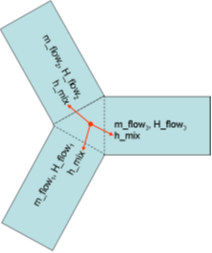
\includegraphics{fluidmix}
  \end{center}
  \caption{Exemplary connection set with three connected components and a common mixing enthalpy.}
\end{figure}

\section{Rationale for inStream}\label{rationale-for-the-formulation-of-the-instream-operator}\label{rationale-for-instream}

For simplicity, the derivation of \lstinline!inStream! is shown at hand of 3 model components that are connected together.
The case for $N$ connections follows correspondingly.

The energy and mass balance equations for the connection set for 3
components are (see above):
\begin{subequations}
\begin{equation}
\begin{split}
0=&\tilde{m}_1\cdot
\begin{cases}
h_{\mathrm{mix}}&\text{if $\tilde{m}_1>0$}\\
h_{\mathrm{outflow},1}&\text{if $\tilde{m}_1 \leq 0$}
\end{cases}\\
+&\tilde{m}_2\cdot
\begin{cases}
h_{\mathrm{mix}}&\text{if $\tilde{m}_2>0$}\\
h_{\mathrm{outflow},2}&\text{if $\tilde{m}_2 \leq 0$}
\end{cases}\\
+&\tilde{m}_3\cdot
\begin{cases}
h_{\mathrm{mix}}&\text{if $\tilde{m}_3>0$}\\
h_{\mathrm{outflow},3}&\text{if $\tilde{m}_3 \leq $}
\end{cases}
\end{split}
\label{eq:D1a}
\end{equation}
\begin{equation}
0=\tilde{m}_1+\tilde{m}_2+\tilde{m}_3
\label{eq:D1b}
\end{equation}
\label{eq:D1}
\end{subequations}

The balance equations are implemented using a $\operatorname{max}$ operator in place of
the piecewise expressions, taking care of the different flow directions:
\begin{subequations}
\begin{equation}
\begin{split}
0=&\operatorname{max}(\tilde{m}_1,0)h_{\mathrm{mix}}-\operatorname{max}(-\tilde{m}_1,0)h_{\mathrm{outflow},1}\\
+&\operatorname{max}(\tilde{m}_2,0)h_{\mathrm{mix}}-\operatorname{max}(-\tilde{m}_2,0)h_{\mathrm{outflow},2}\\
+&\operatorname{max}(\tilde{m}_3,0)h_{\mathrm{mix}}-\operatorname{max}(-\tilde{m}_3,0)h_{\mathrm{outflow},3}
\end{split}
\label{eq:D2a}
\end{equation}

\begin{equation}
\begin{split}
0=&\operatorname{max}(\tilde{m}_1,0)-\operatorname{max}(-\tilde{m}_1,0)\\
+&\operatorname{max}(\tilde{m}_2,0)-\operatorname{max}(-\tilde{m}_2,0)\\
+&\operatorname{max}(\tilde{m}_3,0)-\operatorname{max}(-\tilde{m}_3,0)
\end{split}
\label{eq:D2b}
\end{equation}
\label{eq:D2}
\end{subequations}

Equation \eqref{eq:D2a} is solved for $h_{\mathrm{mix}}$
\begin{equation*}
h_{\mathrm{mix}}=\frac{\operatorname{max}(-\tilde{m}_1,0)h_{\mathrm{outflow},1}+\operatorname{max}(-\tilde{m}_2,0)h_{\mathrm{outflow},2}+\operatorname{max}(-\tilde{m}_3,0)h_{\mathrm{outflow},3}}
{\operatorname{max}(\tilde{m}_1,0)+\operatorname{max}(\tilde{m}_2,0)+\operatorname{max}(\tilde{m}_3,0)}
\end{equation*}
Using \eqref{eq:D2b}, the denominator can be changed to:
\begin{equation*}
h_{\mathrm{mix}}=\frac{\operatorname{max}(-\tilde{m}_1,0)h_{\mathrm{outflow},1}+\operatorname{max}(-\tilde{m}_2,0)h_{\mathrm{outflow},2}+\operatorname{max}(-\tilde{m}_3,0)h_{\mathrm{outflow},3}}
{\operatorname{max}(-\tilde{m}_1,0)+\operatorname{max}(-\tilde{m}_2,0)+\operatorname{max}(-\tilde{m}_3,0)}
\end{equation*}
Above it was shown that an equation of this type does not yield properly
formulated model equations. In the streams concept we therefore decide
to split the energy balance, which consists of different branches
depending on the mass flow direction. Consequently, separate energy
balances are the result; each valid for specific flow directions.

In a model governing equations have to establish the specific enthalpy
of fluid leaving the model based on the specific enthalpy of fluid
flowing into it. Whenever the mixing enthalpy is \emph{used} in a model
it is therefore the mixing enthalpy under the assumption of fluid
flowing into said model.

We establish this quantity using a dedicated operator $\text{\lstinline!inStream!}(h_{\mathrm{outflow},i})=h_{\mathrm{mix}}$ assuming that $\tilde{m}_{i} \geq 0$. This leads to
three different incarnations of ($n$ in the general case). This is
illustrated in the figure below. For the present example of three
components in a connection set, this means the following.
\begin{align*}
\text{\lstinline!inStream!}(h_{\mathrm{outflow},1}) &= \frac{\operatorname{max}(-\tilde{m}_2,0)h_{\mathrm{outflow},2}+\operatorname{max}(-\tilde{m}_3,0)h_{\mathrm{outflow},3}}{\operatorname{max}(-\tilde{m}_2,0)+\operatorname{max}(-\tilde{m}_3,0)}\\
\text{\lstinline!inStream!}(h_{\mathrm{outflow},2}) &= \frac{\operatorname{max}(-\tilde{m}_1,0)h_{\mathrm{outflow},1}+\operatorname{max}(-\tilde{m}_3,0)h_{\mathrm{outflow},3}}{\operatorname{max}(-\tilde{m}_1,0)+\operatorname{max}(-\tilde{m}_3,0)}\\
\text{\lstinline!inStream!}(h_{\mathrm{outflow},3}) &= \frac{\operatorname{max}(-\tilde{m}_1,0)h_{\mathrm{outflow},1}+\operatorname{max}(-\tilde{m}_2,0)h_{\mathrm{outflow},2}}{\operatorname{max}(-\tilde{m}_1,0)+\operatorname{max}(-\tilde{m}_2,0)}
\end{align*}
\begin{figure}[H]
  \begin{center}
    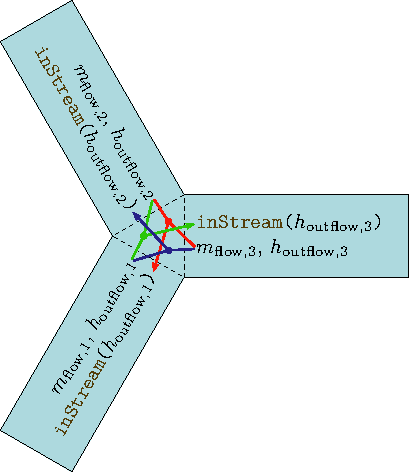
\includegraphics{fluidmix3}
  \end{center}
  \caption{Exemplary connection set with three connected components.}
\end{figure}

In the general case of a connection set with \emph{n} components,
similar considerations lead to the following.
\begin{equation*}
\text{\lstinline!inStream!}(h_{\mathrm{outflow},i})=\frac{\sum_{j=1,\dotsc,n;j\neq i}\operatorname{max}(-\tilde{m}_j,0)h_{\mathrm{outflow},j}}{\sum_{j=1,\dotsc,n;j\neq i}\operatorname{max}(-\tilde{m}_j,0)}
\end{equation*}

\section{Special cases covered by inStream definition}\label{special-cases-covered-by-the-instream-operator-definition}

\subsection{Unconnected stream connector - 1 stream connector}\label{stream-connector-is-not-connected-n-1}\label{unconnected-stream-connector-1-stream-connector}

For this case, the return value of \lstinline!inStream! is arbitrary.
Therefore, it is set to the outflow value.

\subsection{One to one connections - Connection of 2 stream connectors}\label{connection-of-2-stream-connectors-one-to-one-connections-n-2}\label{one-to-one-connections-connection-of-2-stream-connectors}

\begin{align*}
\text{\lstinline!inStream!}(h_{\mathrm{outflow},1}) &= \frac{\operatorname{max}(-\tilde{m}_2,0)h_{\mathrm{outflow},2}}{\operatorname{max}(-\tilde{m}_2,0)}=h_{\mathrm{outflow},2}\\
\text{\lstinline!inStream!}(h_{\mathrm{outflow},2}) &= \frac{\operatorname{max}(-\tilde{m}_1,0)h_{\mathrm{outflow},1}}{\operatorname{max}(-\tilde{m}_1,0)}=h_{\mathrm{outflow},1}
\end{align*}

In this case, \lstinline!inStream! is continuous (contrary to $h_{\mathrm{mix}}$) and does not
depend on flow rates. The latter result means that this transformation
may remove nonlinear systems of equations, which requires that either
simplifications of the form $a * b / a = b$ must be provided, or that this
case is treated directly.

\subsection{Zero mass flow rate - Connection of 3 stream connectors}\label{connection-of-3-stream-connectors-where-one-mass-flow-rate-is-identical-to-zero-n-3-and}\label{zero-mass-flow-rate-connection-of-3-stream-connectors}

The case where $N=3$ and $\tilde{m}_3=0$ occurs when a one-port sensor (like a temperature sensor) is connected to two connected components.
For the sensor, the \lstinline!min! attribute of the mass flow rate should be set to zero (no fluid exiting the component via this connector).
This simplification (and similar ones) can also be used if a tool determines that a mass flow rate is zero or non-negative.
It is also possible to generalize this to the case where more than one sensor is connected.
The suggested implementation results in the following equations, and as indicated the last formula can be simplified further by using $\tilde{m}_3=0$:
\begin{align*}
\text{\lstinline!inStream!}(h_{\mathrm{outflow},1}) &= h_{\mathrm{outflow},2}\\
\text{\lstinline!inStream!}(h_{\mathrm{outflow},2}) &= h_{\mathrm{outflow},1}\\
\text{\lstinline!inStream!}(h_{\mathrm{outflow},3}) &= \frac{\operatorname{max}(-\tilde{m}_1,0)h_{\mathrm{outflow},1}+\operatorname{max}(-\tilde{m}_2,0)h_{\mathrm{outflow},2}}{\operatorname{max}(-\tilde{m}_1,0)+\operatorname{max}(-\tilde{m}_2,0)}\\
&=
\begin{cases}
h_{\mathrm{outflow},2}&\text{if $\tilde{m}_1 \geq 0$}\\
h_{\mathrm{outflow},1}&\text{if $\tilde{m}_1 < 0$ and $\tilde{m}_3 = 0$}
\end{cases}
\end{align*}
\begin{figure}[H]
  \begin{center}
    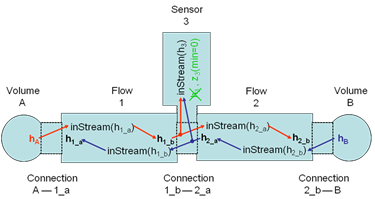
\includegraphics{fluidmix4}
  \end{center}
  \caption{Example series connection of multiple models with stream connectors.}
\end{figure}

For the two components with finite mass flow rates (not the sensor), the
properties discussed for two connected components still hold. The
connection set equations reflect that the sensor does not any influence
by discarding the flow rate of the latter. In several cases a non-linear
equation system is removed by this transformation. However, \lstinline!inStream!
results in a discontinuous equation for the sensor, which is consistent
with modeling the convective phenomena only. The discontinuous equation
is uncritical, if the sensor variable is not used in a feedback loop
with direct feedthrough, since the discontinuous equation is then not
part of an algebraic loop. Otherwise, it is advisable to regularize or
filter the sensor signal.

\subsection{Ideal splitting junction for uni-directional flow - Connection of 3 stream connectors where two mass flow rates are positive}\label{connection-of-3-stream-connectors-where-two-mass-flow-rates-are-positive-ideal-splitting-junction-for-uni-directional-flow}\label{ideal-splitting-junction-for-uni-directional-flow-connection-of-3-stream-connectors-where-two-mass-flow-rates-are-positive}

If uni-directional flow is present and an ideal splitter is modelled,
the required flow direction should be defined in the connector instance
with the \lstinline!min! attribute (the \lstinline!max! attribute could be also defined,
however it does not lead to simplifications):
\begin{lstlisting}[language=modelica]
model m2
  Fluidport c(m_flow(min=0));
  $\ldots$
end m2;
\end{lstlisting}

Consider the case of and all other mass flow rates positive (with the
min attribute set accordingly). Connecting \lstinline!m1.c! with \lstinline!m2.c! and \lstinline!m3.c!, such
that
\begin{lstlisting}[language=modelica]
m2.c.m_flow.min = 0; // max(-m2.c.m_flow,0) = 0
m3.c.m_flow.min = 0; // max(-m3.c.m_flow,0) = 0
\end{lstlisting}
results in the following equation:
\begin{equation*}
\text{\lstinline!inStream!}(h_{\mathrm{outflow},1})=\frac{\operatorname{max}(-\tilde{m}_2,0)h_{\mathrm{outflow},2}+\operatorname{max}(-\tilde{m}_3,0)h_{\mathrm{outflow},3}}{\operatorname{max}(-\tilde{m}_2,0)+\operatorname{max}(-\tilde{m}_3,0)}=\frac{0}{0}
\end{equation*}

\lstinline!inStream! cannot be evaluated for a connector, on which
the mass flow rate has to be negative by definition. The reason is that
the value is arbitrary, which is why it is defined as follows.
\begin{equation*}
\text{\lstinline!inStream!}(h_{\mathrm{outflow},1}):=h_{\mathrm{outflow},1}
\end{equation*}
For the remaining connectors, \lstinline!inStream! reduces to a simple result.
\begin{align*}
\text{\lstinline!inStream!}(h_{\mathrm{outflow},2}) &= \frac{\operatorname{max}(-\tilde{m}_1,0)h_{\mathrm{outflow},1}+\operatorname{max}(-\tilde{m}_3,0)h_{\mathrm{outflow},3}}{\operatorname{max}(-\tilde{m}_1,0)+\operatorname{max}(-\tilde{m}_3,0)}
  = h_{\mathrm{outflow},1}\\
\text{\lstinline!inStream!}(h_{\mathrm{outflow},3}) &= \frac{\operatorname{max}(-\tilde{m}_1,0)h_{\mathrm{outflow},1}+\operatorname{max}(-\tilde{m}_2,0)h_{\mathrm{outflow},2}}{\operatorname{max}(-\tilde{m}_1,0)+\operatorname{max}(-\tilde{m}_2,0)}
  = h_{\mathrm{outflow},1}
\end{align*}
Again, the previous non-linear algebraic system of equations is removed.
This means that utilizing the information about uni-directional flow is
very important.

To summarize, if all mass flow rates are zero, the balance equations for
stream variables \eqref{eq:D1} and for flows \eqref{eq:D2} are identically fulfilled. In
such a case, any value of $h_{\mathrm{mix}}$ fulfills \eqref{eq:D1}, i.e., a unique
mathematical solution does not exist. This specification only requires
that a solution fulfills the balance equations. Additionally, a
recommendation is given to compute all unknowns in a unique way, by
providing an explicit formula for \lstinline!inStream!. Due to the
definition, that only flows where the corresponding \lstinline!min! attribute is
neither zero nor positive enter this formula, a meaningful physcial
result is always obtained, even in case of zero mass flow rate. As a
side effect, non-linear equation systems are automatically removed in
special cases, like sensors or uni-directional flow, without any
symbolic transformations (no equation must be analyzed; only the
\lstinline!min! attributes of the corresponding flow variables).


% Modelica Revision History
\chapter{Modelica Revision History}\doublelabel{modelica-revision-history}

This appendix describes the history of the Modelica Language Design, and
its contributors. This appendix is just present for historic reasons and
is not normative. The current version of this document is available from
\url{https://www.modelica.org/documents}.

\section{Modelica 3.4}\doublelabel{modelica-3-4}
Modelica 3.4 was released April 10, 2017. The Modelica 3.4 specification
was edited by Hans Olsson.

\subsection{Main changes in Modelica 3.4}\doublelabel{main-changes-in-modelica-3-4}

The following Modelica Change Proposals are backward compatible
extensions added in 3.4:

\begin{itemize}
\item
  Automatic conversions between different versions (MCP-0014), 
  \ref{version-handling}. Ticket
  \href{https://trac.modelica.org/Modelica/ticket/1622}{\#1622}.
\item
  Flattening is clearly specified (MCP-0019), \ref{simple-name-lookup} and \ref{flattening-process}.
  Ticket \href{https://trac.modelica.org/Modelica/ticket/1829}{\#1829}.
\item
  Convert from Integer to Enumeration (MCP-0022), primarily 
  \ref{type-conversion-of-integer-to-enumeration-values}. Ticket
  \href{https://trac.modelica.org/Modelica/ticket/1842}{\#1842}.
\item
  Explicitly casting a Model to Record (MCP-0023), \ref{casting-to-record}.
  Ticket \href{https://trac.modelica.org/Modelica/ticket/1953}{\#1953}.
\item
  Initialization of Clocked Continuous States (MCP-0024), 
  \ref{clocked-discrete-time-and-clocked-discretized-continuous-time-partition},
  \ref{initialization-of-clocked-partitions} and \ref{other-operators}. Ticket
  \href{https://trac.modelica.org/Modelica/ticket/2007}{\#2007}.
\item
  An added option to Ellipse Annotation to draw only an arc (MCP-0026),
  \ref{ellipse}. Ticket
  \href{https://trac.modelica.org/Modelica/ticket/2045}{\#2045}.
\item
  Allowing mixed Real and non-Real Record Derivatives (MCP-0028),
  \ref{using-the-derivative-annotation}. Ticket
  \href{https://trac.modelica.org/Modelica/ticket/2134}{\#2134}.
\end{itemize}

The definition of pure functions was refined, in particular to restore
backwards compatibility with Modelica 3.2, \ref{pure-modelica-functions}. Ticket
\href{https://trac.modelica.org/Modelica/ticket/1937}{\#1937}.

The following minor improvements were made (starting from 3.3 Revision
1):

\begin{itemize}
\item
  Clarified simulation model, \ref{scope-of-the-specification}. Ticket
  \href{https://trac.modelica.org/Modelica/ticket/730}{\#730}.
\item
  Clarified structural analysis, \ref{scope-of-the-specification}. Ticket
  \href{https://trac.modelica.org/Modelica/ticket/588}{\#588}.
\item
  Clarified meta-symbols, \ref{notation-and-grammar} and 2.3.1. Ticket
  \href{https://trac.modelica.org/Modelica/ticket/1616}{\#1616}.
\item
  Typo, \ref{identifiers}. Ticket
  \href{https://trac.modelica.org/Modelica/ticket/1702}{\#1702}.
\item
  Clarified newline, \ref{strings}. Ticket
  \href{https://trac.modelica.org/Modelica/ticket/1479}{\#1479}.
\item
  Allow '"' and define it to be equal to '\textbackslash{}"' (and
  similarly for '\textbackslash{}?'), \ref{identifiers}. Ticket
  \href{https://trac.modelica.org/Modelica/ticket/1176}{\#1176}.
\item
  Clarified that built-in functions in the specification, \ref{built-in-intrinsic-operators-with-function-syntax}
  and 12.5. Ticket
  \href{https://trac.modelica.org/Modelica/ticket/1608}{\#1608}.
\item
  Clarified named arguments for builtin operators, in particular
  spatialDistribution, \ref{derivative-and-special-purpose-operators-with-function-syntax} and \ref{positional-or-named-input-arguments-of-functions}. Ticket
  \href{https://trac.modelica.org/Modelica/ticket/2002}{\#2002}.
\item
  Clarified that semiLinear is continuous, \ref{derivative-and-special-purpose-operators-with-function-syntax}. Ticket
  \href{https://trac.modelica.org/Modelica/ticket/112}{\#112}.
\item
  Corrected spelling, \ref{derivative-and-special-purpose-operators-with-function-syntax}. Ticket
  \href{https://trac.modelica.org/Modelica/ticket/1828}{\#1828}.
\item
  Corrected typo in code and reformulated description, \ref{spatialdistribution}.
  Ticket \href{https://trac.modelica.org/Modelica/ticket/1588}{\#1588},
  \href{https://trac.modelica.org/Modelica/ticket/1729}{\#1729}, and
  \href{https://trac.modelica.org/Modelica/ticket/2166}{\#2166}.
\item
  Corrected typo for events, \ref{noevent-and-smooth}. Ticket
  \href{https://trac.modelica.org/Modelica/ticket/1657}{\#1657}.
\item
  Clarified sample operator, \ref{event-related-operators-with-function-syntax}. Ticket
  \href{https://trac.modelica.org/Modelica/ticket/677}{\#677}.
\item
  Additional functions give parameter expression, \ref{parameter-expressions}. Ticket
  \href{https://trac.modelica.org/Modelica/ticket/1082}{\#1082}.
\item
  Clarified ExternalObject, \ref{prefix-rules}. Ticket
  \href{https://trac.modelica.org/Modelica/ticket/1546}{\#1546}.
\item
  Simplified rules type prefixes for structured components, \ref{prefix-rules}. Ticket
  \href{https://trac.modelica.org/Modelica/ticket/1686}{\#1686}.
\item
  Clarified that unexpanded bindings shall be unexpanded, \ref{acyclic-bindings-of-constants-and-parameters}.
  Ticket \href{https://trac.modelica.org/Modelica/ticket/2153}{\#2153}.
\item
  Clarified conditional components, \ref{conditional-component-declaration}. Ticket
  \href{https://trac.modelica.org/Modelica/ticket/2057}{\#2057}.
\item
  Improved example to avoid using class, \ref{local-class-definitions-nested-classes}. Ticket
  \href{https://trac.modelica.org/Modelica/ticket/553}{\#553}.
\item
  Clarify inheritance from predefines types, \ref{specialized-classes}. Ticket
  \href{https://trac.modelica.org/Modelica/ticket/1250}{\#1250}.
\item
  Allow connector inheriting from operator record, \ref{specialized-classes}. Ticket
  \href{https://trac.modelica.org/Modelica/ticket/1714}{\#1714}.
\item
  Clarify restrictions on record components, \ref{specialized-classes}. Ticket
  \href{https://trac.modelica.org/Modelica/ticket/1615}{\#1615}.
\item
  Clarify that only functions may have external clause, \ref{specialized-classes} and
  \ref{function-as-a-specialized-class}. Ticket
  \href{https://trac.modelica.org/Modelica/ticket/2014}{\#2014}.
\item
  Clarified equation count for operator record, \ref{balanced-models}. Ticket
  \href{https://trac.modelica.org/Modelica/ticket/866}{\#866}.
\item
  Clarified restriction on attributes, \ref{predefined-types-and-classes}. Ticket
  \href{https://trac.modelica.org/Modelica/ticket/1426}{\#1426}.
\item
  Clarified how reserved the different built-in types are, \ref{predefined-types-and-classes}.
  Ticket \href{https://trac.modelica.org/Modelica/ticket/1538}{\#1538}.
\item
  Removed restriction on nominal and explained purpose, \ref{real-type}.
  Ticket \href{https://trac.modelica.org/Modelica/ticket/1445}{\#1445}.
\item
  Added unbounded to Real, \ref{real-type} and \ref{attributes-start-fixed-nominal-and-unbounded}. Ticket
  \href{https://trac.modelica.org/Modelica/ticket/926}{\#926}.
\item
  Added fixed-attribute for String, \ref{string-type}. Ticket
  \href{https://trac.modelica.org/Modelica/ticket/1797}{\#1797}.
\item
  Clarified and corrected example in \ref{enumeration-types}. Ticket
  \href{https://trac.modelica.org/Modelica/ticket/1849}{\#1849} and
  \href{https://trac.modelica.org/Modelica/ticket/2150}{\#2150}.
\item
  Clarified nominal attribute, \ref{attributes-start-fixed-nominal-and-unbounded} 
  and \ref{stream-operator-instream-and-connection-equations}. Ticket
  \href{https://trac.modelica.org/Modelica/ticket/1877}{\#1877}.
\item
  Added that Connections is builtin package, \ref{connections}. Ticket
  \href{https://trac.modelica.org/Modelica/ticket/1883}{\#1883}.
\item
  Clarified lookup-order regarding import, \ref{simple-name-lookup}. Ticket
  \href{https://trac.modelica.org/Modelica/ticket/1573}{\#1573}.
\item
  Extend calling functions through component to array case, \ref{composite-name-lookup} and \ref{expressions}. Ticket
  \href{https://trac.modelica.org/Modelica/ticket/1613}{\#1613}.
\item
  Clarified existing use of automatic inner declarations, \ref{instance-hierarchy-name-lookup-of-inner-declarations}
  and \ref{annotations-for-the-graphical-user-interface}. Ticket
  \href{https://trac.modelica.org/Modelica/ticket/1551}{\#1551} and
  \href{https://trac.modelica.org/Modelica/ticket/1749}{\#1749}.
\item
  Removed restriction on array size for modifiers, \ref{interface-compatibility-or-subtyping}. Ticket
  \href{https://trac.modelica.org/Modelica/ticket/1432}{\#1432}.
\item
  Clarified that 2/3 and 2\^{}(-3) are Real, \ref{type-compatible-expressions}. Ticket
  \href{https://trac.modelica.org/Modelica/ticket/1647}{\#1647}.
\item
  Clarified that external declaration is inherited, \ref{inheritance-extends-clause}. Ticket
  \href{https://trac.modelica.org/Modelica/ticket/789}{\#789}.
\item
  Further clarified order for multiple inheritance, \ref{instantiation} and
  \ref{inheritance-extends-clause}. Ticket
  \href{https://trac.modelica.org/Modelica/ticket/2015}{\#2015}.
\item
  Clarified inheritance restrictions, \ref{restrictions-on-the-kind-of-base-class}. Ticket
  \href{https://trac.modelica.org/Modelica/ticket/1451}{\#1451}.
\item
  Restricted merging of modifiers, \ref{merging-of-modifications}. Ticket
  \href{https://trac.modelica.org/Modelica/ticket/791}{\#791}.
\item
  Clarified each especially for nested arrays, \ref{single-modification} and \ref{modifiers-for-array-elements}.
  Ticket \href{https://trac.modelica.org/Modelica/ticket/1596}{\#1596}.
\item
  Clarified replaceable with array sizes on types, \ref{redeclaration}. Ticket
  \href{https://trac.modelica.org/Modelica/ticket/1251}{\#1251}.
\item
  Corrected and moved example, \ref{redeclaration} and \ref{constraining-type}. Ticket
  \href{https://trac.modelica.org/Modelica/ticket/1034}{\#1034}.
\item
  Clarified "redeclare class extends B", \ref{the-class-extends-redeclaration-mechanism}. Ticket
  \href{https://trac.modelica.org/Modelica/ticket/462}{\#462} and
  \href{https://trac.modelica.org/Modelica/ticket/709}{\#709}.
\item
  Corrected example, \ref{constraining-type}. Ticket
  \href{https://trac.modelica.org/Modelica/ticket/1725}{\#1725}.
\item
  Clarified description and annotation on constraining-clause, \ref{constraining-clause-annotations}. Ticket
  \href{https://trac.modelica.org/Modelica/ticket/512}{\#512}.
\item
  Corrected typo, \ref{annotation-choices-for-suggested-redeclarations-and-modifications}. Ticket
  \href{https://trac.modelica.org/Modelica/ticket/1770}{\#1770}.
\item
  Clarified for-equation with types, \ref{for-equations-repetitive-equation-structures}. Ticket
  \href{https://trac.modelica.org/Modelica/ticket/915}{\#915}.
\item
  Clarified event generation, \ref{events-and-synchronization}. Ticket
  \href{https://trac.modelica.org/Modelica/ticket/2114}{\#2114}.
\item
  Further clarified initial() for when-clauses, \ref{initialization-initial-equation-and-initial-algorithm} -- and
  indicated that this appendix is not normative. Ticket
  \href{https://trac.modelica.org/Modelica/ticket/1852}{\#1852}.
\item
  Clarified using start-attribute for parameters, \ref{initialization-initial-equation-and-initial-algorithm}. Ticket
  \href{https://trac.modelica.org/Modelica/ticket/2136}{\#2136}.
\item
  Clarified that states for first order ODE, \ref{the-number-of-equations-needed-for-initialization}. Ticket
  \href{https://trac.modelica.org/Modelica/ticket/937}{\#937}.
\item
  Clarified adding input/output prefix for expandable connector
  variables, \ref{expandable-connectors}. Ticket
  \href{https://trac.modelica.org/Modelica/ticket/829}{\#829}.
\item
  Clarified creating elements in expandable connectors, \ref{expandable-connectors}.
  Ticket \href{https://trac.modelica.org/Modelica/ticket/428}{\#428}.
\item
  Corrected expandable connector example, \ref{expandable-connectors}. Ticket
  \href{https://trac.modelica.org/Modelica/ticket/1763}{\#1763}.
\item
  Clarified that stream-variables do not generate equations, \ref{generation-of-connection-equations}. Ticket
  \href{https://trac.modelica.org/Modelica/ticket/1584}{\#1584}.
\item
  Restrict that stream only connects to stream, \ref{restrictions-of-connections-and-connectors}. Ticket
  \href{https://trac.modelica.org/Modelica/ticket/796}{\#796}.
\item
  Clarified section heading, \ref{balancing-restriction-and-size-of-connectors}. Ticket
  \href{https://trac.modelica.org/Modelica/ticket/727}{\#727}.
\item
  Clarified vector arguments for operators in \ref{overconstrained-equation-operators-for-connection-graphs}. Ticket
  \href{https://trac.modelica.org/Modelica/ticket/1590}{\#1590}.
\item
  Corrected example, \ref{an-overdetermined-connector-for-power-systems}. Ticket
  \href{https://trac.modelica.org/Modelica/ticket/2143}{\#2143}.
\item
  Clarified return type for reduction expressions, \ref{reduction-functions-and-operators}.
  Ticket \href{https://trac.modelica.org/Modelica/ticket/981}{\#981}.
\item
  Extended reduction expression sum to operator records, \ref{reduction-functions-and-operators}.
  Ticket \href{https://trac.modelica.org/Modelica/ticket/1897}{\#1897}.
\item
  Clarified table in \ref{reduction-expressions}. Ticket
  \href{https://trac.modelica.org/Modelica/ticket/1722}{\#1722}.
\item
  Match parenthesis, \ref{array-constructor-with-several-iterators}. Ticket
  \href{https://trac.modelica.org/Modelica/ticket/1558}{\#1558}.
\item
  Recommend better alternative for generating vector, \ref{vector-construction}.
  Ticket \href{https://trac.modelica.org/Modelica/ticket/1837}{\#1837}.
\item
  Defined unary operators, \ref{array-element-wise-addition-subtraction-and-string-concatenation}. Ticket
  \href{https://trac.modelica.org/Modelica/ticket/2027}{\#2027}.
\item
  Allow missing trailing indices, sections \ref{array-indexing} and \ref{slice-operation}. Ticket
  \href{https://trac.modelica.org/Modelica/ticket/1603}{\#1603}.
\item
  Clarified that element-wise division gives real result, 
  \ref{array-element-wise-division}. Ticket
  \href{https://trac.modelica.org/Modelica/ticket/1119}{\#1119}.
\item
  Removed misleading comment, \ref{execution-of-an-algorithm-in-a-model}. Ticket
  \href{https://trac.modelica.org/Modelica/ticket/938}{\#938}.
\item
  Clarified how assignment works for multi-returning functions, 
  \ref{assignments-from-called-functions-with-multiple-results}. Ticket
  \href{https://trac.modelica.org/Modelica/ticket/1921}{\#1921}.
\item
  Clarified no equations and initial algorithms in functions, 
  \ref{function-as-a-specialized-class}. Ticket
  \href{https://trac.modelica.org/Modelica/ticket/2160}{\#2160}.
\item
  Clarified assigning to record variables with bindings in functions,
  \ref{function-as-a-specialized-class}. Ticket
  \href{https://trac.modelica.org/Modelica/ticket/2016}{\#2016}.
\item
  Clarified initialization of variables in functions, \ref{initialization-and-declaration-assignments-of-components-in-functions}.
  Ticket \href{https://trac.modelica.org/Modelica/ticket/1708}{\#1708}.
\item
  Standarize current practice of using = instead of := for bindings in
  functions, \ref{function-as-a-specialized-class}. Ticket
  \href{https://trac.modelica.org/Modelica/ticket/1595}{\#1595}.
\item
  Clarified function partial evaluation, \ref{function-partial-application}. Ticket
  \href{https://trac.modelica.org/Modelica/ticket/647}{\#647}.
\item
  Clarified initialization of record components in functions, 
  \ref{initialization-and-declaration-assignments-of-components-in-functions}. Ticket
  \href{https://trac.modelica.org/Modelica/ticket/1230}{\#1230}.
\item
  Clarified flexible array sizes, \ref{flexible-array-sizes-and-resizing-of-arrays-in-functions}. Ticket
  \href{https://trac.modelica.org/Modelica/ticket/2158}{\#2158}.
\item
  Clarified name of output for record constructor in \ref{record-constructor-functions}.
  Ticket \href{https://trac.modelica.org/Modelica/ticket/366}{\#366}.
\item
  Clarified derivatives for functions in several ways, \ref{using-the-derivative-annotation}.
  Ticket \href{https://trac.modelica.org/Modelica/ticket/985}{\#985},
  \href{https://trac.modelica.org/Modelica/ticket/1543}{\#1543},
  \href{https://trac.modelica.org/Modelica/ticket/1544}{\#1544},
  \href{https://trac.modelica.org/Modelica/ticket/1545}{\#1545},
  \href{https://trac.modelica.org/Modelica/ticket/1547}{\#1547},
  \href{https://trac.modelica.org/Modelica/ticket/1548}{\#1548},
  \href{https://trac.modelica.org/Modelica/ticket/1788}{\#1788},
  \href{https://trac.modelica.org/Modelica/ticket/1972}{\#1972},
  \href{https://trac.modelica.org/Modelica/ticket/1987}{\#1987}.
\item
  Clarified that using C89 and added possibility for C89, C99, and C11 ,
  \ref{external-function-interface}. Ticket
  \href{https://trac.modelica.org/Modelica/ticket/1088}{\#1088}.
\item
  Clarified input/output to external functions, \ref{external-function-interface}. Ticket
  \href{https://trac.modelica.org/Modelica/ticket/775}{\#775}.
\item
  Clarified handling of Boolean variables for external C, 
  \ref{simple-types}. Ticket
  \href{https://trac.modelica.org/Modelica/ticket/1846}{\#1846}.
\item
  Added that Strings can be sent to FORTRAN 77, \ref{simple-types}. Ticket
  \href{https://trac.modelica.org/Modelica/ticket/1971}{\#1971}.
\item
  Allow multiple include directories, \ref{annotations-for-external-libraries-and-include-files}. Ticket
  \href{https://trac.modelica.org/Modelica/ticket/2103}{\#2103}.
\item
  Allow specific libraries for different compiler versions, 
  \ref{annotations-for-external-libraries-and-include-files}. Ticket
  \href{https://trac.modelica.org/Modelica/ticket/1316}{\#1316}.
\item
  Added external warning functions, \ref{utility-functions}. Ticker
  \href{https://trac.modelica.org/Modelica/ticket/1967}{\#1967}.
\item
  Clarified that pointers are only valid during each call, \ref{external-objects}. Ticket
  \href{https://trac.modelica.org/Modelica/ticket/1611}{\#1611}.
\item
  Clarified constructor and destructor, \ref{external-objects}. Ticket
  \href{https://trac.modelica.org/Modelica/ticket/1907}{\#1907}.
\item
  Clarified 'structured entity' to be 'directory', \ref{mapping-package-class-structures-to-a-hierarchical-file-system}.
  Ticket \href{https://trac.modelica.org/Modelica/ticket/922}{\#922}.
\item
  Clarified handling of incorrect package.order, \ref{mapping-a-package-class-hierarchy-into-a-directory-hierarchy-structured-entity}.
  Ticket \href{https://trac.modelica.org/Modelica/ticket/1858}{\#1858}.
\item
  Restricted use of files with multiple classes, \ref{mapping-a-package-class-hierarchy-into-a-single-file-nonstructured-entity}.
  Ticket \href{https://trac.modelica.org/Modelica/ticket/1854}{\#1854}.
\item
  Clarified storing resources in a file-system, \ref{external-resources}. Ticket
  \href{https://trac.modelica.org/Modelica/ticket/685}{\#685},
  \href{https://trac.modelica.org/Modelica/ticket/1623}{\#1623}.
\item
  Used correct font, \ref{external-resources}. Ticket
  \href{https://trac.modelica.org/Modelica/ticket/2061}{\#2061}.
\item
  Clarified that inStream optimizations are allowed, \ref{stream-operator-instream-and-connection-equations}.
  Ticket \href{https://trac.modelica.org/Modelica/ticket/1766}{\#1766}.
\item
  Corrected actualStream example in \ref{stream-operator-actualstream}. Ticket
  \href{https://trac.modelica.org/Modelica/ticket/1652}{\#1652}.
\item
  Corrected non-periodic rational clocks, \ref{clock-constructors}. Ticket
  \href{https://trac.modelica.org/Modelica/ticket/2022}{\#2022}.
\item
  Clarified initialization of clocked discretized continuous-time
  partitions, \ref{solver-methods}. Ticket
  \href{https://trac.modelica.org/Modelica/ticket/1528}{\#1528}.
\item
  Defined rendering order, \ref{annotations-for-graphical-objects}. Ticket
  \href{https://trac.modelica.org/Modelica/ticket/1750}{\#1750}.
\item
  Clarified rotation direction, \ref{common-definitions}. Ticket
  \href{https://trac.modelica.org/Modelica/ticket/1830}{\#1830}.
\item
  Clarified coordinate system definition, \ref{coordinate-systems}. Ticket
  \href{https://trac.modelica.org/Modelica/ticket/1831}{\#1831}.
\item
  Defined coordinate system inheritance to be less suprising, 
  \ref{coordinate-systems} and \ref{extends-clause}. Ticket
  \href{https://trac.modelica.org/Modelica/ticket/1978}{\#1978}.
\item
  Clarified lineThickness and borderPattern, \ref{graphical-primitives} \ref{graphical-properties}.
  Ticket \href{https://trac.modelica.org/Modelica/ticket/1896}{\#1896}.
\item
  Corrected formatting, \ref{graphical-properties}. Ticket
  \href{https://trac.modelica.org/Modelica/ticket/1825}{\#1825}.
\item
  Made the different Text-annotations more similar, \ref{connections}.
  Ticket \href{https://trac.modelica.org/Modelica/ticket/1621}{\#1621}.
\item
  Clarified LinePatterns in \ref{graphical-primitives}. Ticket
  \href{https://trac.modelica.org/Modelica/ticket/1483}{\#1483}.
\item
  Corrected flipping of components and bitmaps, and clarified various
  aspects of bitmaps, \ref{component-instance} and \ref{bitmap}. Ticket
  \href{https://trac.modelica.org/Modelica/ticket/1923}{\#1923}.
\item
  Clarified arrows, \ref{line}. Ticket
  \href{https://trac.modelica.org/Modelica/ticket/1894}{\#1894}.
\item
  Clarified existing use of zero-width texts, \ref{text}. Ticket
  \href{https://trac.modelica.org/Modelica/ticket/1636}{\#1636}.
\item
  Added specific fontnames, \ref{text}. Ticket
  \href{https://trac.modelica.org/Modelica/ticket/1986}{\#1986}.
\item
  Added alternative for macro-expansion, \ref{text}. Ticket
  \href{https://trac.modelica.org/Modelica/ticket/2148}{\#2148}.
\item
  Corrected example in \ref{mouse-input}. Ticket
  \href{https://trac.modelica.org/Modelica/ticket/2111}{\#2111}.
\item
  Placed annotation last in classes, in particular \ref{annotations-for-the-graphical-user-interface}. Ticket
  \href{https://trac.modelica.org/Modelica/ticket/1009}{\#1009}.
\item
  Cleaned up code and formatting in \ref{annotations-for-the-graphical-user-interface}. Ticket
  \href{https://trac.modelica.org/Modelica/ticket/2041}{\#2041},
  \href{https://trac.modelica.org/Modelica/ticket/2042}{\#2042}, and
  \href{https://trac.modelica.org/Modelica/ticket/2125}{\#2125}.
\item
  Added missing nano-prefix, \ref{the-syntax-of-unit-expressions}. Ticket
  \href{https://trac.modelica.org/Modelica/ticket/1261}{\#1261}.
\item
  Replaced the outdated contents of \ref{the-modelica-standard-library} by a hyperlink. Ticket
  \href{https://trac.modelica.org/Modelica/ticket/2130}{\#2130}.
\item
  Added ModelicaServices to \ref{the-modelica-standard-library}. Ticket
  \href{https://trac.modelica.org/Modelica/ticket/2132}{\#2132}.
\item
  Restrict grammar to avoid modifiers with leading dot, \ref{grammar}.
  Ticket \href{https://trac.modelica.org/Modelica/ticket/1027}{\#1027}.
\item
  Restrict grammar for base-prefix, \ref{class-definition}. Ticket
  \href{https://trac.modelica.org/Modelica/ticket/917}{\#917}.
\item
  Restrict grammar for arrays, \ref{expressions}. Ticket
  \href{https://trac.modelica.org/Modelica/ticket/809}{\#809}.
\item
  Restrict grammar for function arguments (replacing semantic
  restriction), \ref{expressions}. Ticket
  \href{https://trac.modelica.org/Modelica/ticket/1634}{\#1634}.
\item
  Corrected typo in \ref{rationale-for-the-formulation-of-the-instream-operator}. Ticket
  \href{https://trac.modelica.org/Modelica/ticket/1317}{\#1317}.
\end{itemize}

\subsection{Contributors to the Modelica Language 3.4}\doublelabel{contributors-to-the-modelica-language-3-4}

The members of the Modelica Association contributed to the Modelica 3.4
specification.

\section{Modelica 3.3 Revision 1}\doublelabel{modelica-3-3-revision-1}

Modelica 3.3 Revision 1 was released July 11, 2014. The Modelica 3.3
Revision 1 specification was edited by Hans Olsson.

\subsection{Main changes in Modelica 3.3 Revision 1}\doublelabel{main-changes-in-modelica-3-3-revision-1}
The changes made in Modelica 3.2 Revision 2 are included, and in
addition the following improvements were made:

\begin{itemize}
\item
  Clarified that String-operator cannot use positional arguments,
  \ref{numeric-functions-and-conversion-functions}. Ticket
  \href{https://trac.modelica.org/Modelica/ticket/1468}{\#1468}.
\item
  Corrected size of enumeration, \ref{numeric-functions-and-conversion-functions} and \ref{type-conversion-of-enumeration-values-to-string-or-integer}. Ticket
  \href{https://trac.modelica.org/Modelica/ticket/1369}{\#1369}.
\item
  Clarified spatialDistribution, \ref{built-in-mathematical-functions-and-external-built-in-functions}. Ticket
  \href{https://trac.modelica.org/Modelica/ticket/1510}{\#1510}.
\item
  Restricted cardinality to give a clear definition, \ref{cardinality-deprecated}.
  Ticket \href{https://trac.modelica.org/Modelica/ticket/1409}{\#1409}.
\item
  Clarified which constants need a value, \ref{constant-expressions}. Ticket
  \href{https://trac.modelica.org/Modelica/ticket/1220}{\#1220}.
\item
  Clarified type prefixes rules, \ref{prefix-rules}. Tickets
  \href{https://trac.modelica.org/Modelica/ticket/1196}{\#1196},
  \href{https://trac.modelica.org/Modelica/ticket/1221}{\#1221},
  \href{https://trac.modelica.org/Modelica/ticket/1301}{\#1301}.
\item
  Added exception for cyclic parameter bindings (already used in MSL),
  \ref{acyclic-bindings-of-constants-and-parameters}. Ticket
  \href{https://trac.modelica.org/Modelica/ticket/1320}{\#1320}.
\item
  Added example for use of conditional components, \ref{conditional-component-declaration}. Ticket
  \href{https://trac.modelica.org/Modelica/ticket/1227}{\#1227}.
\item
  Corrected annotation-grammar, \ref{class-declarations}. Ticket
  \href{https://trac.modelica.org/Modelica/ticket/1378}{\#1378}.
\item
  Corrected duplicated class-definition grammar, \ref{class-declarations}. Ticket
  \href{https://trac.modelica.org/Modelica/ticket/1388}{\#1388}.
\item
  Clarified short class definition, \ref{short-class-definitions}. Ticket
  \href{https://trac.modelica.org/Modelica/ticket/527}{\#527}.
\item
  Removed unusable variant for operator and operator function, \ref{specialized-classes}. Ticket
  \href{https://trac.modelica.org/Modelica/ticket/1459}{\#1459},
  \href{https://trac.modelica.org/Modelica/ticket/1497}{\#1497}.
\item
  Added definition of AssertionLevel, \ref{assertionlevel}. ticket
  \href{https://trac.modelica.org/Modelica/ticket/962}{\#962}.
\item
  Corrected typos at end of loops in examples,\ref{enumeration-types} and
  \ref{implicit-iteration-ranges-of-for-equations}. Ticket
  \href{https://trac.modelica.org/Modelica/ticket/902}{\#902}
\item
  Clarified temporary flattening, \ref{composite-name-lookup}. Ticket
  \href{https://trac.modelica.org/Modelica/ticket/1327}{\#1327}.
\item
  Added definition of modification equations, \ref{modifications}. Ticket
  \href{https://trac.modelica.org/Modelica/ticket/959}{\#959}.
\item
  Clarified modifiers for array elements, \ref{modifiers-for-array-elements}. Ticket
  \href{https://trac.modelica.org/Modelica/ticket/1324}{\#1324}.
\item
  Corrected example for final element modification, \ref{final-element-modification-prevention}
  Ticket \href{https://trac.modelica.org/Modelica/ticket/1326}{\#1326}.
\item
  Corrected duplicated class-definition grammar, \ref{the-class-extends-redeclaration-mechanism}. Ticket
  \href{https://trac.modelica.org/Modelica/ticket/1388}{\#1388}.
\item
  Clarified modifiers on constraining type, \ref{constraining-type}. Ticket
  \href{https://trac.modelica.org/Modelica/ticket/1033}{\#1033}.
\item
  Clarified when redeclare can be used with the same type and rules for
  redeclaring array types, \ref{restrictions-on-redeclarations}. Tickets
  \href{https://trac.modelica.org/Modelica/ticket/1252}{\#1252},
  \href{https://trac.modelica.org/Modelica/ticket/1281}{\#1281}.
\item
  Clarified default for annotation choicesAllMatching, \ref{annotation-choices-for-suggested-redeclarations-and-modifications}.
  Ticket \href{https://trac.modelica.org/Modelica/ticket/1391}{\#1391}.
\item
  Forbid when-statements in initial equation/algorithm (they would in
  most cases not be active; leading to confusion), \ref{restrictions-on-equations-within-when-equations} and
  \ref{restrictions-on-when-statements}. Ticket
  \href{https://trac.modelica.org/Modelica/ticket/1288}{\#1288}.
\item
  Clarified reinit during initialization, \ref{reinit} \ref{initialization-initial-equation-and-initial-algorithm}. Ticket
  \href{https://trac.modelica.org/Modelica/ticket/1372}{\#1372}.
\item
  Clarified using start-values as guess-values; \ref{initialization-initial-equation-and-initial-algorithm}. Tickets
  \href{https://trac.modelica.org/Modelica/ticket/1133}{\#1133},
  \href{https://trac.modelica.org/Modelica/ticket/1246}{\#1246}.
\item
  Clarified allowed use of variables in expandable connectors; \ref{expandable-connectors}. Ticket
  \href{https://trac.modelica.org/Modelica/ticket/1279}{\#1279}.
\item
  Clarified causality for expandable connectors; \ref{expandable-connectors}. Ticket
  \href{https://trac.modelica.org/Modelica/ticket/1305}{\#1305}.
\item
  Clarified expandable connectors in general; \ref{expandable-connectors}. Ticket
  \href{https://trac.modelica.org/Modelica/ticket/1330}{\#1330}.
\item
  Clarified connection matching, \ref{restrictions-of-connections-and-connectors}. Ticket
  \href{https://trac.modelica.org/Modelica/ticket/884}{\#884}.
\item
  Added quantity checks for connectors (MSL already relies on this
  check); \ref{restrictions-of-connections-and-connectors}. Ticket
  \href{https://trac.modelica.org/Modelica/ticket/1284}{\#1284}.
\item
  Clarified arrays with non-Integer dimensions, \ref{array-declarations}. Ticket
  \href{https://trac.modelica.org/Modelica/ticket/1501}{\#1501}.
\item
  Clarified that ndims is allow for a scalar, \ref{array-dimension-and-size-functions}. Ticket
  \href{https://trac.modelica.org/Modelica/ticket/1303}{\#1303}.
\item
  Clarified number of arguments for zeros, ones, fill, \ref{specialized-array-constructor-functions}.
  Ticket \href{https://trac.modelica.org/Modelica/ticket/1351}{\#1351}.
\item
  Clarified min/max, \ref{reduction-functions-and-operators}. Ticket
  \href{https://trac.modelica.org/Modelica/ticket/1036}{\#1036}.
\item
  Clarified array expressions using iterations allow non-simple types,
  \ref{array-constructor-with-iterators}. Ticket
  \href{https://trac.modelica.org/Modelica/ticket/1521}{\#1521}.
\item
  Clarified arrays with non-Integer dimensions, \ref{indexing-with-boolean-or-enumeration-values}. Ticket
  \href{https://trac.modelica.org/Modelica/ticket/1463}{\#1463}.
\item
  Clarified calling function as specialized class, \ref{function-as-a-specialized-class}. Ticket
  \href{https://trac.modelica.org/Modelica/ticket/1362}{\#1362}.
\item
  Clarified default values in functions depending on other inputs,
  \ref{positional-or-named-input-arguments-of-functions}. Ticket
  \href{https://trac.modelica.org/Modelica/ticket/1346}{\#1346}.
\item
  Corrected syntax error in example, \ref{function-partial-application}. Ticket
  \href{https://trac.modelica.org/Modelica/ticket/1338}{\#1338}.
\item
  Clarified annotations on external functions, \ref{external-function-interface}. Ticket
  \href{https://trac.modelica.org/Modelica/ticket/660}{\#660}.
\item
  Add possibility for sending arrays in records to external functions,
  \ref{external-function-interface}. Ticket
  \href{https://trac.modelica.org/Modelica/ticket/351}{\#351}.
\item
  Corrected spelling to FORTRAN 77, \ref{aliasing}. Ticket
  \href{https://trac.modelica.org/Modelica/ticket/1278}{\#1278}.
\item
  Clarified default directories, \ref{annotations-for-external-libraries-and-include-files}. Ticket
  \href{https://trac.modelica.org/Modelica/ticket/1456}{\#1456}.
\item
  Clarified constructing/destructing external objects, \ref{external-objects}.
  Ticket \href{https://trac.modelica.org/Modelica/ticket/1518}{\#1518}.
\item
  Clarified encapsulation requirement for operator record, \ref{overloaded-operators}.
  Ticket \href{https://trac.modelica.org/Modelica/ticket/1254}{\#1254}.
\item
  Clarified operator record: arrays, priority, and zero result, 
  \ref{overloaded-binary-operations}. Tickets
  \href{https://trac.modelica.org/Modelica/ticket/1469}{\#1469},
  \href{https://trac.modelica.org/Modelica/ticket/1476}{\#1476},
  \href{https://trac.modelica.org/Modelica/ticket/1481}{\#1481}.
\item
  Added element wise operations for operator record, \ref{overloaded-binary-operations}.
  Ticket \href{https://trac.modelica.org/Modelica/ticket/1455}{\#1455}.
\item
  Improved formulation, \ref{clock-constructors}. Ticket
  \href{https://trac.modelica.org/Modelica/ticket/1362}{\#1362}.
\item
  Clarified why noClock exists; \ref{sub-clock-conversion-operators}. Ticket
  \href{https://trac.modelica.org/Modelica/ticket/1094}{\#1094}.
\item
  Added initial conditions to solver methods for clocked discretized
  continuous-time partitions; \ref{solver-methods}. Ticket
  \href{https://trac.modelica.org/Modelica/ticket/1379}{\#1379}.
\item
  Added requirement that priorities must be unique for statechart
  transitions (the restriction was present in original description and
  is necessary to ensure deterministic behavior), \ref{state-machine-semantics}. Ticket
  \href{https://trac.modelica.org/Modelica/ticket/853}{\#853}.
\item
  Corrected syntax in Line definition, \ref{line}. Ticket
  \href{https://trac.modelica.org/Modelica/ticket/1464}{\#1464}.
\item
  Corrected connectorSizing description, \ref{annotations-for-the-graphical-user-interface}. Ticket
  \href{https://trac.modelica.org/Modelica/ticket/1441}{\#1441}.
\item
  Corrected license example, \ref{licensing}. Ticket
  \href{https://trac.modelica.org/Modelica/ticket/1127}{\#1127}.
\item
  Clarified names of productions in grammar and changed to use hyphen,
  \ref{lexical-conventions}. Tickets
  \href{https://trac.modelica.org/Modelica/ticket/713}{\#713} and
  \href{https://trac.modelica.org/Modelica/ticket/1033}{\#1033}.
\item
  Modified grammar use consistent style for import-list, \ref{class-definition}.
  Ticket \href{https://trac.modelica.org/Modelica/ticket/1374}{\#1374}.
\end{itemize}

\subsection{Contributors to the Modelica Language, Version 3.3 Revision 1}\doublelabel{contributors-to-the-modelica-language-version-3-3-revision-1}

The following members of the Modelica Association contributed to the
Modelica 3.3 Revision 1 and/or Modelica 3.2 Revision 2 specification
(alphabetical list):

\begin{longtable}{p{0.3cm}p{14cm}}
&Peter Aronsson, MathCore AB, Linköping, Sweden\\
&Peter Fritzson, PELAB, Linköping University, Linköping, Sweden\\
&Hilding Elmqvist, Dassault Systèmes, Lund, Sweden\\
&Christoph Höger, Technical University of Berlin, Berlin, Germany\\
&Gerd Kurzbach, ITI GmbH, Dresden, Germany\\
&Jesper Mattsson, Modelon AB, Lund, Sweden\\
&Hans Olsson, Dassault Systèmes, Lund, Sweden\\
&Martin Otter, DLR, Oberpfaffenhofen, Germany\\
&Adrian Pop, Linköping University, Linköping, Sweden\\
&Elena Shmoylova, Maplesoft, Waterloo, Canada\\
&Martin Sjölund, PELAB, Linköping University, Linköping, Sweden\\
&Stefan Vorkoetter, Maplesoft, Waterloo, Canada
\end{longtable}

\section{Modelica 3.3}\doublelabel{modelica-3-3}

Modelica 3.3 was released on May 9, 2012. The Modelica 3.3 specification
was edited by Hans Olsson, Hilding Elmqvist and Martin Otter.

\subsection{Main changes in Modelica 3.3}\doublelabel{main-changes-in-modelica-3-3}

The following \textbf{backward compatible extensions} have been
introduced with Modelica 3.3:

\begin{itemize}
\item
  Language elements for describing synchronous behavior suited for
  implementation of control systems, \ref{synchronous-language-elements}.
\item
  Language elements to define synchronous state machines, \ref{state-machines}.
\item
  The spatialDistribution function for special one-dimensional flow
  problems, \ref{spatialdistribution}.
\item
  The getInstanceName function for diagnostic messages, \ref{getinstancename}.
\item
  Possible to call a function through an instance name, \ref{composite-name-lookup}.
\item
  Can use the start-value for a parameter to give a non-zero default
  that should be changed, \ref{initialization-initial-equation-and-initial-algorithm}.
\item
  A recommened procedure for priority between initial values have been
  added, \ref{recommended-selection-of-start-values}.
\item
  Functions can be defined without algorithm-section, \ref{function-as-a-specialized-class}.
\item
  Functions can be marked as pure or impure with specified semantics,
  \ref{pure-modelica-functions}.
\item
  The rules for ExternalObject have been clarified, \ref{external-objects} and
  \ref{interface-or-type-relationships}.
\item
  Multiple definition import, \ref{importing-definitions-from-a-package}.
\item
  Additional annotations allowing:

  \begin{itemize}
  \item
    Functions to generate events, \ref{annotations-for-code-generation}.
  \item
    Experiments to specify a time-resolution of simulation result,
    \ref{annotations-for-simulation-experiments}.
  \item
    Single instance of class, \ref{annotation-for-single-use-of-class}.
  \item
    Text in the diagram layer can use a macro syntax, \ref{text}.
  \item
    Color selection dialog for parameters, \ref{annotations-for-the-graphical-user-interface}.
  \item
    Conversion to specify a set of versions to convert with one script,
    \ref{version-handling}.
  \item
    Licensed libraries to define the set of allowed operations
    (including binary/source export), \ref{licensing}.
  \end{itemize}
\end{itemize}

The following \textbf{changes} in Modelica 3.3 are \textbf{not}
\textbf{backwards compatible}:

\begin{itemize}
\item
  \ref{synchronous-language-elements} ``Mapping of Models to Execution Environments'' from
  Modelica 3.2 has been removed (a more powerful functionality is
  instead provided with the new \ref{synchronous-language-elements} and \ref{state-machines}). Since, no
  released tools has yet supported the previous \ref{synchronous-language-elements}, this not
  backwards compatible change is uncritical.
\item
  The new spatialDistribution and getInstanceName functions could cause
  problems if another function with that name was already used.
\end{itemize}

\begin{itemize}
\item
  Conditional physical connectors must be connected if enabled, 
  \ref{conditional-component-declaration} 
  and \ref{restrictions-of-connections-and-connectors}. In almost all cases they have to be connected
  to generate correct result, and it is not possible to check that they
  are connected in the models
\end{itemize}

\subsection{Contributors to Modelica 3.3}\doublelabel{contributors-to-modelica-3-3}

The language elements for describing synchronous behavior, \ref{synchronous-language-elements},
was mainly developed by Hilding Elmqvist, Martin Otter, and Sven Erik
Mattsson. Hilding Elmqvist wrote a detailed tutorial. Sven Erik Mattsson
developed a test implementation of the language elements and the needed
new algorithms. Based on the prototype, tests and feedback have been
provided by Martin Otter and Bernhard Thiele.

The language elements to define synchronous state machines, \ref{state-machines},
was mainly developed by Hilding Elmqvist with contributions from
Francois Dupont, Sven Erik Mattsson and Fabien Gaucher. Hilding Elmqvist
wrote a tutorial. Sven Erik Mattsson and Carl-Fredrik Abelson developed
a test implementation. Based on the prototype, tests and feedback have
been provided by Alain Thura, Emmanuel Ledinot, Claire Campan, and
Martin Malmheden.

The spatialDistribution operator was initiated by Hubertus Tummescheit,
based on an operator of Dymola, and with contributions from Hans Olsson.

The improved definition of pure and impure functions and the enhanced
import statement was proposed by Peter Fritzson.

The various smaller language improvements based on submitted tickets
have been developed by a group headed by Hans Olsson and with group
members Peter Fritzson, Christoph Höger, Gerd Kurzbach, Jesper Mattsson,
Martin Sjölund, and Stefan Vorkoetter.

The following members of the Modelica Association participated at design
meetings and contributed to the Modelica 3.3 specification:

\begin{longtable}{p{0.3cm}p{14cm}}
&Johan Åkesson, Lund University and Modelon AB, Lund, Sweden\\
&Peter Aronsson, MathCore AB, Linköping, Sweden\\
&Ingrid Bausch-Gall, BAUSCH-GALL GmbH, Munich, Germany\\
&Volker Beuter, Kämmerer AG, Germany\\
&Torsten Blochwitz, ITI GmbH, Dresden, Germany\\
&David Broman, PELAB, Linköping University, Sweden\\
&Dag Brück, Dassault Systèmes, Lund, Sweden\\
&Francesco Casella, Politecnico di Milano, Milano, Italy\\
&Christoph Clauss, Fraunhofer, Dresden, Germany\\
&Mike Dempsey, Claytex Services Limited, Leamington Spa, U.K.\\
&Karin Dietl, TU Hamburg-Harburg, Germany\\
&Francois Dupont, Dassault Systèmes, Brest, France\\
&Jonas Eborn, Modelon, Lund, Sweden\\
&Hilding Elmqvist, Dassault Systèmes, Lund, Sweden\\
&Guilioano Fontanella, AIT, Vienna, Austria\\
&Rüdiger Franke, ABB Power Generation, Mannheim, Germany\\
&Peter Fritzson, PELAB, Linköping University, Sweden\\
&Sébastien Furic, LMS International, Roanne. France\\
&Leo Gall, BAUSCH-GALL Gmbh, Munich, Germany\\
&Peter Harman, deltatheta uk limited, U.K.\\
&Anton Haumer, AIT, Vienna, Austria\\
&Dan Henriksson, Dassault Systèmes, Lund, Sweden\\
&Christoph Höger, TU Berlin, Berlin, Germany\\
&Christian Kral, AIT, Vienna, Austria\\
&Gerd Kurzbach, ITI GmbH, Dresden, Germany\\
&Kilian Link, Siemens AB, Erlangen, Germany\\
&Krisitin Majetta, Fraunhofer, Dresden, Germany\\
&Martin Malmheden, Dassault Systèmes, Velicy, France\\
&Jesper Mattsson, Modelon, Lund, Sweden\\
&Sven Erik Mattsson, Dassault Systèmes, Lund, Sweden\\
&Eric Neuber, ITI GmbH, Dresden, Germany\\
&Ramine Nikoukhah, Altair, France\\
&Hans Olsson, Dassault Systèmes, Lund, Sweden\\
&Martin Otter, DLR-RM (German Aerospace Center), Oberpfaffenhofen,Germany\\
&Peter Pepper, Fraunhofer FIRST, Berlin, Germany\\
&Adrian Pop, Linköping University, Linköping, Sweden\\
&Olena Rogovchenko, PELAB, Linköping, Sweden\\
&Stefan-Alexander Schneider, BMW, Munich, Germany\\
&Michael Sielemann, German Aerospace Center, Oberpfaffenhofen, Germany\\
&Martin Sjölund, PELAB; Linköping, Sweden\\
&Kristian Stavåker, PELAB, Linköping, Sweden\\
&Bernhard Thiele, DLR-RM (German Aerospace Center), Oberpfaffenhofen,Germany\\
&Eric Thomas, Dassault Aviation, Paris, France\\
&Michael Tiller, Dassault Systèmes, Velicy, France\\
&Hubertus Tummescheit, Modelon AB, Lund, Sweden\\
&Andreas Uhlig, ITI, Dresden Germany\\
&Vladimir Vukovic, AIT, Vienna, Germany\\
&Stefan Vorkoetter, Maplesoft, Waterloo, Canada\\
&Daniel Weil, Dassault Systèmes, Grenoble, France\\
&Hans-Jürg Wiesmann, ABB Switzerland, Corporate Research, Baden,Switzerland\\
&Dietmar Winkler, Telemark University College, Porsgrunn, Norway\\
&Stefan Wischhusen, XRG Simulation, Hamburg, Germany\\
&Dirk Zimmer, DLR-RM (German Aerospace Center), Oberpfaffenhofen, Germany
\end{longtable}

\subsection{Acknowledgments}\doublelabel{acknowledgments1}

For the design of the synchronous language elements (\ref{synchronous-language-elements}) and
synchronous state machines (\ref{state-machines}), and for the understanding of
fine details of synchronous languages, especially from Lucid Synchrone,
very helpful discussions with

\begin{longtable}{p{0.3cm}p{14cm}}
&Albert Benveniste, IRISA/INRIA, Rennes, France\\
&Marc Pouzet, Laboratoire d'Informatique de l'ENS, Paris\\
&Benoit Caillaud, IRISA, Rennes, France\\
&Timothy Bourke, INRIA, Rennes, France
\end{longtable}
are appreciated.

\section{Modelica 3.2 Revision 2}\doublelabel{modelica-3-2-revision-2}

Modelica 3.2 Revision 2 was released 2013. The Modelica 3.2 Revision 2
specification was edited by Hans Olsson and Martin Otter.

\subsection{Main changes in Modelica 3.2 Revision 2}\doublelabel{main-changes-in-modelica-3-2-revision-2}

The Modelica language was slightly adapted (in a backwards compatible
way -- except as listed below) in order that the Modelica Standard
Library (MSL) version 3.2.1 is fully compliant to Modelica Language 3.2
Revision 2. This required the following improvements compared to 3.2
Revision 1:

\begin{itemize}
\item
  Possible to call a function through an instance name, \ref{composite-name-lookup}\\
  (used in MSL 3.2 to compute the gravity acceleration in
  Modelica.Mechanics.MultiBody.World; this feature was also introduced
  in Modelica Language version 3.3 in May 2012).
\item
  New built-in operator Connections.rooted(A.R) to inquire whether an
  overdetermined type or record instance A.R in a call to
  Connections.branch(A.R,B.R) is closer to the root of the spanning tree
  than B.R, \ref{overconstrained-equation-operators-for-connection-graphs} (used in MSL 3.2 to avoid algebraic loops in
  several components such as in
  Modelica.Mechanics.MultiBody.Joints.Revolute).
\item
  Several new annotations where vendor-specific variants were used in
  MSL 3.2; \ref{annotation-choices-for-suggested-redeclarations-and-modifications}, 
  \ref{annotations-for-documentation}, \ref{annotations-for-code-generation}, 
  \ref{annotations-for-simulation-experiments}, \ref{connections}, and \ref{annotations-for-the-graphical-user-interface}.
\item
  Specified that Evaluate can also occur in types, since this is used in
  MSL and important for performance; \ref{annotations-for-code-generation}. Ticket
  \href{https://trac.modelica.org/Modelica/ticket/925}{\#925}.
\item
  Macros in graphical text items, \ref{text}. Ticket
  \href{https://trac.modelica.org/Modelica/ticket/659}{\#659}. (This
  feature was also introduced in Modelica Language version 3.3.)
\item
  Initial equations are discrete -- used in MSL for initialization of
  pre-variables, \ref{discrete-time-expressions}. Ticket
  \href{https://trac.modelica.org/Modelica/ticket/853}{\#853}.
\item
  Updated noDerivative to be consistent with MSL, \ref{using-the-derivative-annotation}. This
  is an incompatibility -- but the other variant was not used. Ticket
  \href{https://trac.modelica.org/Modelica/ticket/1035}{\#1035}.
\item
  Clarified handling of component with missingInnerMessage; 
  \ref{annotations-for-the-graphical-user-interface}. Ticket
  \href{https://trac.modelica.org/Modelica/ticket/891}{\#891}.
\item
  Clarified definition of protected; \ref{access-control-public-and-protected-elements}. Ticket
  \href{https://trac.modelica.org/Modelica/ticket/975}{\#975},
  \href{https://trac.modelica.org/Modelica/ticket/1123}{\#1123}.
\end{itemize}

In addition several issues with the specification text were corrected:

\begin{itemize}
\item
  Clarified an unclear sequence regarding functions as input arguments
  in \ref{prefix-rules}. Ticket
  \href{https://trac.modelica.org/Modelica/ticket/1182}{\#1182}.
\item
  Clarified allowed binding equations for redeclarations, \ref{balanced-models}.
  Ticket \href{https://trac.modelica.org/Modelica/ticket/1111}{\#1111}.
\item
  Unspecified enumerations now have defined semantics, \ref{unspecified-enumeration}.
  Ticket \href{https://trac.modelica.org/Modelica/ticket/834}{\#834}.
\item
  Transitively non-Replaceable, \ref{transitively-non-replaceable}. Ticket
  \href{https://trac.modelica.org/Modelica/ticket/854}{\#854}.
\item
  Modification text improved to not refer to inherited class, 
  \ref{modifications}. Ticket
  \href{https://trac.modelica.org/Modelica/ticket/1042}{\#1042}.
\item
  Precedence for modifiers on constraining-clause clarified, \ref{constraining-type}. Ticket
  \href{https://trac.modelica.org/Modelica/ticket/1128}{\#1128}.
\item
  Clarified arrays for constraining type, \ref{constraining-type}. Ticket
  \href{https://trac.modelica.org/Modelica/ticket/1148}{\#1148}.
\item
  Avoid all forms of connections depending on connections, 
  \ref{connect-equations}. Ticket
  \href{https://trac.modelica.org/Modelica/ticket/828}{\#828}.
\item
  Clarified equation count for if-equations, \ref{if-equations}. Ticket
  \href{https://trac.modelica.org/Modelica/ticket/888}{\#888}.
\item
  Complete definition of reinit, \ref{reinit}. Ticket
  \href{https://trac.modelica.org/Modelica/ticket/578}{\#578}. This
  forbids reinit in algorithms -- but it was previously not
  well-defined.
\item
  Clarified initializaton of pre(vc) for a non-discrete (that is
  continuous-time) Real variable vc, \ref{initialization-initial-equation-and-initial-algorithm}. Ticket
  \href{https://trac.modelica.org/Modelica/ticket/1195}{\#1195}.
\item
  Only one way of handling arrays of connectors is now defined, 
  \ref{connectors-and-connections}. Ticket \href{https://trac.modelica.org/Modelica/ticket/757}{\#757}.
\item
  Example now use correct sine-source, \ref{connect-equations-and-connectors}. Ticket
  \href{https://trac.modelica.org/Modelica/ticket/750}{\#750}.
\item
  Restricted parameters in connectors, \ref{restrictions-of-connections-and-connectors}. Ticket
  \href{https://trac.modelica.org/Modelica/ticket/768}{\#768}.
\item
  Clarified type restrictions for some operators, \ref{reduction-functions-and-operators},
  \ref{matrix-and-vector-algebra-functions}. Ticket
  \href{https://trac.modelica.org/Modelica/ticket/622}{\#622}.
\item
  Clarified that if at least one array element is used on the left hand
  side of the assignment operator in an algorithm section, then the
  complete array is initialized in this section, \ref{execution-of-an-algorithm-in-a-model}. Ticket
  \href{https://trac.modelica.org/Modelica/ticket/1190}{\#1190}.
\item
  Record constructor corrected to not refer to keywords that should not
  occur, \ref{record-constructor-functions}. Ticket
  \href{https://trac.modelica.org/Modelica/ticket/907}{\#907}.
\item
  External storage of classes, \ref{mapping-a-package-class-hierarchy-into-a-single-file-nonstructured-entity}, 
  \ref{the-within-clause} and \ref{mapping-of-versions-to-file-system}.
  Tickets \href{https://trac.modelica.org/Modelica/ticket/1019}{\#1019},
  \href{https://trac.modelica.org/Modelica/ticket/892}{\#892},
  \href{https://trac.modelica.org/Modelica/ticket/887}{\#887}.
\item
  Added example and explanation for inheritance restriction on operator
  record; \ref{example-of-overloading-for-complex-numbers}. Ticket
  \href{https://trac.modelica.org/Modelica/ticket/1065}{\#1065}.
\item
  Chapter ``Mapping of Models to Execution Environments'' was removed;
  this change was already decided for Modelica 3.3 and no tool had
  released an implementation of this feature. Ticket
  \href{https://trac.modelica.org/Modelica/ticket/1015}{\#1015}.
\item
  Corrected license-example in \ref{licensing}. Ticket
  \href{https://trac.modelica.org/Modelica/ticket/1127}{\#1127}.
\item
  Grammar was internally restructured for short-class-definition,
  \ref{class-declarations}, \ref{class-definition}. Ticket
  \href{https://trac.modelica.org/Modelica/ticket/1140}{\#1140}.
\end{itemize}

\subsection{Contributors to the Modelica Language, Version 3.2 Revision 2}\doublelabel{contributors-to-the-modelica-language-version-3-2-revision-2}

The following members of the Modelica Association contributed to the
Modelica 3.2 Revision 2 specification (alphabetical list):

Peter Aronsson, MathCore AB, Linköping, Sweden

Peter Fritzson, PELAB, Linköping University, Linköping, Sweden

Hilding Elmqvist, Dassault Systèmes, Lund, Sweden

Christoph Höger, Technical University of Berlin, Berlin, Germany

Gerd Kurzbach, ITI GmbH, Dresden, Germany

Jesper Mattsson, Modelon AB, Lund, Sweden

Hans Olsson, Dassault Systèmes, Lund, Sweden

Martin Otter, DLR, Oberpfaffenhofen, Germany

Adrian Pop, Linköping University, Linköping, Sweden

Elena Shmoylova, Maplesoft, Waterloo, Canada

Martin Sjölund, PELAB, Linköping University, Linköping, Sweden

Stefan Vorkoetter, Maplesoft, Waterloo, Canada

\section{Modelica 3.2 Revision 1}\doublelabel{modelica-3-2-revision-1}

Modelica 3.2 Revision 1 was released on Feb. 29, 2012. The Modelica 3.2
Revision 1 specification was edited by Hans Olsson and Peter Fritzson.

\subsection{Main changes in Modelica 3.2 Revision 1}\doublelabel{main-changes-in-modelica-3-2-revision-1}

The Modelica language was not changed with respect to the previous
version 3.2. Only issues with the specification text have been fixed. In
particular:

\begin{itemize}
\item
  Corrected typos and improved formatting.
\item
  \ref{comments} Comments:\\
  There are 2 and not 3 kinds of comments and comments are treated as
  white space character.\\
  Added definition of white space character.
\item
  \ref{identifiers} Identifiers:\\
  The single quotes are part of the identifier, e.g., 'x'.
\item
  \ref{built-in-variable-time} Built-in Variable time:\\
  Variable "time" is only available in models and blocks and not in the
  other classes.
\item
  \ref{built-in-mathematical-functions-and-external-built-in-functions} Built-in Mathematical Functions\\
  Definition of "atan2" corrected.
\item
  \ref{derivative-and-special-purpose-operators-with-function-syntax} Special Purpose Operators\\
  Included definition of inStream and actualStream operators from
  \ref{stream-connectors}.
\item
  \ref{event-related-operators-with-function-syntax} Event-Related Operators\\
  Clarified, that the first argument of "smooth" is a scalar.\\
  Improved the definition of "reinit".
\item
  \ref{discrete-time-expressions} Discrete-Time Expressions\\
  Improved definition of ordered relations
  (\textgreater{},\textless{},\textgreater{}=,\textless{}=).
\item
  \ref{conditional-component-declaration} Conditional Component Declaration\\
  Clarified redeclaration of a component.
\item
  \ref{specialized-classes} Specialized Classes\\
  Clarified that "stream" cannot be used in a record.\\
  Clarified restrictions on elements in a "connector".\\
  Errors in example of operator record Complex corrected.
\item
  \ref{enumeration-types} Enumeration Types\\
  Error in example corrected.
\item
  \ref{simultaneous-inner-outer-declarations} Simulataneous Inner/Outer Declarations\\
  Clarified inner/outer declarations.
\item
  \ref{inheritance-extends-clause} Inheritance\\
  Clarified that the elements of a flattened base class are added at the
  place of the extends clause.\\
  Equations of the flattened base class that are syntactically
  equivalent to equations in the flattened enclosing class are
  deprecated.
\item
  \ref{modifications} Modifications\\
  Element modifiers are no longer part of language, reference grammar
  instead of duplicating it.
\item
  \ref{redeclaration} Redeclaration\\
  Improved redeclarations definition and moved an example from \ref{the-class-extends-redeclaration-mechanism} at
  the right place.
\item
  \ref{reinit} reinit\\
  Improved reinit definition.
\item
  \ref{initialization-initial-equation-and-initial-algorithm} Initialization\\
  Clarified that only when-clauses with restricted form of initial() as
  condition will be active during initialization.
\item
  \ref{reduction-expressions} Reduction Expressions\\
  Improved definition
\item
  \ref{types-as-iteration-ranges} Types as iteration ranges\\
  Newly introduced section to improve the definition of iteration ranges
\item
  \ref{function-as-a-specialized-class} Function\\
  Added missing restrictions that model, block, inner, outer cannot be
  used in a function.
\item
  \ref{positional-or-named-input-arguments-of-functions} Positional or Named Input Arguments of Functions\\
  Corrected formal syntax of a function call
\item
  \ref{initialization-and-declaration-assignments-of-components-in-functions} Initialization and Declaration Assignments of
  Components in Functions\\
  Added the restriction of acylic bindings.
\item
  \ref{records} Records\\
  Mapping of arrays in records to C-structs is removed.
\item
  \ref{bitmap} Bitmap\\
  Defined flipping more precisely.
\item
  \ref{lexical-conventions} Lexical conventions\\
  More precisely defined whitespace and comments.
\item
  \ref{grammar} Grammar\\
  Improved/corrected grammar definition
\end{itemize}

\subsection{Contributors to the Modelica Language, Version 3.2 Revision 1}\doublelabel{contributors-to-the-modelica-language-version-3-2-revision-1}

The following members of the Modelica Association contributed to the
Modelica 3.2 Revision 1 specification (alphabetical list):

Peter Aronsson, MathCore AB, Linköping, Sweden

Peter Fritzson, PELAB, Linköping University, Linköping, Sweden

Christoph Höger, Technical University of Berlin, Berlin, Germany

Gerd Kurzbach, ITI GmbH, Dresden, Germany

Jesper Mattsson, Modelon AB, Lund, Sweden

Hans Olsson, Dassault Systèmes, Lund, Sweden

Adrian Pop, Linköping University, Linköping, Sweden

Martin Sjölund, PELAB, Linköping University, Linköping, Sweden

Stefan Vorkoetter, Maplesoft, Waterloo, Canada

\section{Modelica 3.2}\doublelabel{modelica-3-2}

Modelica 3.2 was released on March 24, 2010. The Modelica 3.2
specification was edited by Hans Olsson, Martin Otter and others.

\subsection{Main changes in Modelica 3.2}\doublelabel{main-changes-in-modelica-3-2}

The following \textbf{backward compatible extensions} have been
introduced with Modelica 3.2:

\begin{itemize}
\item
  Homotopy function for making it easier to solve initialization
  problems (see \ref{derivative-and-special-purpose-operators-with-function-syntax}).
\item
  Functions as formal inputs to functions (see new \ref{functional-input-arguments-to-functions}).
\item
  Overloaded operators have been refined (see \ref{overloaded-operators}):

  \begin{itemize}
  \item
    A new specialized class ``operator record'' is introduced -- with
    specialized typing rules (the type is identified by the class name;
    all other Modelica classes have a structural type system where the
    type is only defined by the public elements). Overloaded operators
    can only be defined inside an ``operator record''. This change fixes
    a flaw in Modelica 3.1, since the look-up of overloaded operators is
    performed by the record class name.
  \item
    Inheritance of an ``operator record'' is allowed if defined via a
    short class definition. This removes a restriction of operator
    overloading in Modelica 3.1, e.g., to define derived classes with
    units for the record elements, like deriving ComplexVoltage from
    Complex.
  \item
    New overloaded element `0' in order that operator record classes can
    be used as flow variables in connectors.
  \end{itemize}
\item
  Unicode support in description strings, strings in annotations and in
  comments in order to improve Modelica, e.g., for Arabian, Asian or
  Indian users (see grammar changes in \ref{lexical-conventions}). Modelica files are
  UTF-8 encoded, and can start with the UTF-8 encoded byte order mark
  (0xef 0xbb 0xbf) to indicate that it may contain UTF-8 characters;
  this is treated as white-space in the grammar (see \ref{mapping-a-package-class-hierarchy-into-a-single-file-nonstructured-entity}).
\item
  Constants can once again be modified unless declared final -- as this
  is already used in packages.\\
  (see \ref{constant-expressions}).
\item
  Global name lookup has been introduced (e.g.
  ``.Modelica.Constants.pi''), see \ref{global-name-lookup}.
\item
  New C-functions ModelicaVFormatMessage and ModelicaVFormatError, to
  simplify message formatting in external functions (see \ref{utility-functions})
\item
  Additional annotations allowing:

  \begin{itemize}
  \item
    Inclusion of C-header and object library files in packages and
    referencing them with URIs.\\
    (new annotations IncludeDirectory, LibraryDirectory, and
    standardized platform names like win32; see \ref{annotations-for-external-libraries-and-include-files}; resolves
    ticket \#297).
  \item
    Images in parameter dialogs (new annotation groupImage; see 
    \ref{annotations-for-the-graphical-user-interface}).
  \item
    Start and fixed attributes for variables in parameter dialogs\\
    (new annotation showStartAttribute; see \ref{annotations-for-the-graphical-user-interface}).
  \item
    Access control for packages to protect intelectual property.\\
    (new annotations Protection, and License; see new \ref{annotations-for-access-control-to-protect-intellectual-property}).
  \end{itemize}
\end{itemize}

The following \textbf{changes} in Modelica 3.2 are \textbf{not}
\textbf{backwards compatible}:

\begin{itemize}
\item
  The new built-in operator name ``homotopy''. In rare cases this might
  give name clashes in existing models.
\item
  Records with overloaded operations must be declared as ``operator
  record'' instead of as ``record''. This is uncritical because tools
  that already support operator overloading will support the Modelica
  3.1 form still for some time.
\end{itemize}

\subsection{Contributors to the Modelica Language, Version 3.2}\doublelabel{contributors-to-the-modelica-language-version-3-2}

The initial version of ``functions as formal inputs to functions'' was
proposed by Peter Fritzson.

The definition of header-files and object-libraries with the
``IncludeDirectory'' and ``LibraryDirectory'' annotations was mainly
developed by Hans Olsson.

The Protection annotation used for access control is an improved version
of existing annotations from Dymola. The License annotation was mainly
developed by Dag Brück with improvements from Magnus Gäfvert.

The flaw in the operator overloading concept was detected by Sébastien
Furic. He also proposed the basic fix, by using a nominal type system
for records with overloaded operations.

The global name lookup was proposed by Stefan Vorkoetter.

The support for Unicode was initiated by Rui Gao and Hoyoun Kim.\\
The "homotopy" operator was proposed by Martin Otter, Michael Sielemann
and Francesco Casella. Michael Sielemann demonstrated with benchmark
problems that non-linear solvers are not able to solve reliably
initialization problems and that the homotopy operator is therefore
needed. He provided a prototype implementation of the homotopy-operator
and demonstrated its use on a vehicle dynamics example. Utilizing the
prototype implementation, Francesco Casella demonstrated with a model of
a thermal power plant with 390 iteration variables of the initialization
problem, that an appropriate usage of the homotopy operator allows to
reliably initialize the system without providing guess values for the
iteration variables. This was a strong indication that the homotopy
operator will indeed improve initialization in Modelica significantly.

The following members of the Modelica Association participated at design
meetings and contributed to the Modelica 3.2 specification:

Johan Åkesson, Lund University and Modelon AB, Lund, Sweden

Peter Aronsson, MathCore AB, Linköping, Sweden

Bernhard Bachmann, University of Applied Sciences, Bielefeld, Germany

Jonathan Beck, Dassault Systèmes, Paris, France

Torsten Blochwitz, ITI GmbH, Dresden, Germany

David Broman, PELAB, Linköping University, Sweden

Dag Brück, Dassault Systèmes, Lund, Sweden

Francesco Casella, Politecnico di Milano, Milano, Italy

Mike Dempsey, Claytex Services Limited, Leamington Spa, U.K.

Karin Dietl, TU Hamburg-Harburg, Germany

Filippo Donida, Politecnico di Milano, Milano, Italy

Hilding Elmqvist, Dassault Systèmes, Lund, Sweden

Peter Fritzson, PELAB, Linköping University, Sweden

Sébastien Furic, LMS International, Roanne. France

Manuel Gräber, TU Braunschweig, Germany

Peter Harman, deltatheta uk limited, U.K.

Anton Haumer, AIT, Vienna, Austria

Carsten Heinrich, Institut für Luft- und Kältetechnik, Dresden, Germany

Dan Henriksson, Dassault Systèmes, Lund, Sweden

Fredrik Karlsson, PELAB, Linköping University, Sweden

Christian Kral, AIT, Vienna, Austria

Imke Krüger, TU Hamburg-Harburg, Hamburg, Germany

Gerd Kurzbach, ITI GmbH, Dresden, Germany

Kilian Link, Siemens AB, Erlangen, Germany

Sven Erik Mattsson, Dassault Systèmes, Lund, Sweden

Eric Neuber, ITI GmbH, Dresden, Germany

Hans Olsson, Dassault Systèmes, Lund, Sweden

Martin Otter, German Aerospace Center, Oberpfaffenhofen, Germany

Adrian Pop, Linköping University, Linköping, Sweden

Katrin Prölß, Modelon AB, Lund, Sweden

Michael Sielemann, German Aerospace Center, Oberpfaffenhofen, Germany

Bernhard Thiele, German Aerospace Center, Oberpfaffenhofen, Germany

Thorben Vahlenkamp, XRG Simulation, Hamburg, Germany

Eric Thomas, Dassault Aviation, Paris, France

Michael Tiller, Emmeskay, Plymouth, MI, U.S.A

Hubertus Tummescheit, Modelon AB, Lund, Sweden

Stefan Vorkoetter, Maplesoft, Waterloo, Canada

Hans-Jürg Wiesmann, ABB Switzerland, Corporate Research, Baden,
Switzerland

Dietmar Winkler, Telemark University College, Porsgrunn, Norway

\subsection{Acknowledgments}\doublelabel{acknowledgments2}

Partial financial support for the development of Modelica 3.2 by the
following funding agencies has been received:

\begin{itemize}
\item
  The German Ministry BMBF has partially funded DLR, Fraunhofer and
  Siemens (BMBF Förderkennzeichen: 01IS07022F) within the ITEA2 project
  EUROSYSLIB (\url{http://www.eurosyslib.com}).
\item
  The German Ministry BMBF has partially funded ITI GmbH (BMBF
  Förderkennzeichen: 01IS08002K), and the Swedish funding agency VINNOVA
  has partially funded Dynasim (2008-02291), within the ITEA2 project
  MODELISAR
  (\url{http://www.itea2.org/public/project_leaflets/MODELISAR_profile_oct-08.pdf}).
\item
  The Swedish funding agency VINNOVA has partially funded Linköping
  University (PELAB) within the ITEA2 project OPENPROD
  (http://www.openprod.org).
\item
  The Swedish Research Council has partially funded Linköping University
  (PELAB) within the project ``High-Level Debugging of Equation-Based
  System Modeling \& Simulation Languages''.
\item
  The German Ministry BMBF has partially funded FH Bielefeld (BMBF
  Förderkennzeichen: 01IS09029C) within the ITEA2 project OPENPROD
  (\href{http://www.openprod.}{http://www.openprod.org}).
\end{itemize}

\section{Modelica 3.1}\doublelabel{modelica-3-1}

Modelica 3.1 was released on May 27, 2009. The Modelica 3.1
specification was edited by Francesco Casella, Rüdiger Franke, Hans
Olsson, Martin Otter, and Michael Sielemann.

\subsection{Main changes in Modelica 3.1}\doublelabel{main-changes-in-modelica-3-1}

The following \textbf{backward compatible extensions} have been
introduced with Modelica 3.1:

\begin{itemize}
\item
  Overloading of operators like `+' or `*' to allow convenient usage of
  user-defined data structures like complex numbers, polynomials,
  transfer functions. Usually, only scalar operations for one data type
  need to be overloaded. All other needed operations, like operations
  between different data types or on arrays of the new data type, can be
  automatically constructed by the tool.
\item
  Stream connector concept to ensure efficient and reliable simulation
  of fluid systems.
\item
  Partitioning models in parts and mapping these parts to execution
  environments. This allows convenient definition of, e.g.,
  Model-in-the-Loop, Software-in-the-Loop, Hardware-in-the-Loop
  Simulation, from the same ``logical'' system, by inheriting from the
  logical system and setting configuration options.
\item
  Arrays in buses (expandable connector) are much better supported.
  Furthermore, variables declared in an expandable connector need not to
  be referenced in the model and are then not available in the
  simulation model.
\item
  The order of classes stored in separate files can be given.
\item
  A restriction of balanced models was removed, so that modifiers to
  connector and record instances can be used and are considered for the
  equation count. This allows, e.g., a much easier implementation of the
  support connector of the Modelica.Mechanics.Rotational/Translational
  libraries.
\item
  A tool that uses missingInnerMessage to give information may also
  automatically use the corresponding inner-component.
\item
  URIs can be used for links in html-documentation and for the Bitmap
  annotation (such as: ``modelica://Modelica.Mechanics/C.jpg'' for image
  ``C.jpg'' that is stored in the directory of package
  Modelica.Mechanics). This allows to store resources in a package on
  persistent storage and to reference resources via package and resource
  names.
\item
  \emph{Annotation} ``connectorSizing'' to automatically enlarge a
  vector of connectors and connect to a free element of this vector when
  a connection line is drawn. This allows to improve the user
  convenience, especially for state machine and fluid models.
\item
  \emph{Annotation} ``inverse'' to define inverses of functions. This
  allows a tool to solve non-linear algebraic loops by using the
  user-provided inverse function.
\item
  \emph{Annotations} ``versionDate'', ``versionBuild'',
  ``dateModified'', ``revisionId'' to improve version handling. For
  example, this allows handling of maintenance (bug-fix) releases and
  gives a library developer the possibility to state that a particular
  ``build'' is needed for a used library.
\end{itemize}

The following \textbf{defects} have been \textbf{fixed} in the Modelica
specification:

\begin{itemize}
\item
  Modifier with subscripts were previously allowed, but not clearly
  defined, not implemented in many tools, and not used in libraries.
  They were thus removed.
\item
  Modelica keywords (\ref{modelica-keywords}) updated.
\item
  Clarification: Exponentiation and array range operator are
  non-associative\\
  (x\^{}y\^{}z or a:b:c:d:e:f are not allowed; parentheses are required)
\item
  Clarification: Restrictions on combining base classes (\ref{restriction-on-combining-base-classes-and-other-elements}).
\item
  Clarification: Execution of an algorithm (new \ref{execution-of-an-algorithm-in-a-model}).
\item
  The default type for arrays sent to external functions has been
  clarified.
\item
  The ``iconTransformation'' defaults to the (diagram)
  ``transformation'', as was originally the intention.
\item
  The Connection set section was rewritten:

  \begin{itemize}
  \item
    Connection set is clearly defined including examples.
  \item
    The handling of connections involving outer components was rewritten
    to ensure that models that seem to have the same connection
    structure generate the same equations from the connect equations.
    Previously a connection between an outer component and an outside
    connector would move the connection upwards. The implication of this
    movement was unclear: if it turned the connector into an inside
    connector (as was likely the intention) it would prohibit
    default-connection of this normal connector leading to
    counter-intuitive results; and otherwise it would have no impact.
  \end{itemize}
\item
  Example of using fields was corrected.
\item
  Example with MatrixGain was corrected.
\item
  Ambiguous annotations after external-declarations were corrected (as
  already used).
\item
  The reinit-operator can be used multiple times in one algorithm, and
  the semantics clarified.
\item
  Made clearer that acyclic parameters also hold for one parameter
  equation.
\item
  Changed in the text ``attributes'' to ``prefix'', if a prefix is
  meant.
\end{itemize}

The following \textbf{changes} in Modelica 3.1 are not \textbf{backwards
compatible}:

\begin{itemize}
\item
  A class-level annotation can only be placed before the end-statement.
  This is uncritical because tools can easily fix incorrect models
  (ignore this new rule when reading a model and use this rule when
  storing the model).
\item
  New Modelica keywords ``stream'' and ``operator'', a new built-in
  package ``Subtask'' and new-built-in operators ``inStream'' and
  ``actualStream'' have been introduced. In rare cases this might give
  name clashes in existing models.
\item
  Modifiers on declared variables in expandable connectors are no longer
  allowed. This should be uncritical, because expandable connectors are
  usually used for signal buses where the signal is communicated to the
  bus from a block with a connect equation.
\end{itemize}

\subsection{Contributors to the Modelica Language, Version 3.1}\doublelabel{contributors-to-the-modelica-language-version-3-1}

The concept of operator overloading was developed by Hans Olsson, based
on work of Dag Brück, Peter Fritzson, and Martin Otter.

The streams concept was developed by Rüdiger Franke based on work from
Francesco Casella and with contributions especially from Hilding
Elmqvist, Sven Erik Mattson, Hans Olsson, Martin Otter and Michael
Sielemann.

The concept to map models to execution environments was developed by
Hilding Elmqvist, Dan Henriksson, Martin Otter, Bernhard Thiele and Sven
Erik Mattson.

The following members of the Modelica Association participated at design
meetings and contributed to the Modelica 3.1 specification:

Johan Akesson, Lund University and Modelon AB, Lund, Sweden

Johan Andreasson, Modelon AB, Lund, Sweden

Peter Aronsson, MathCore AB, Linköping, Sweden

Bernhard Bachmann , University of Applied Sciences, Bielefeld, Germany

Torsten Blochwitz, ITI GmbH, Dresden, Germany

David Broman, Linköping University, Linköping, Sweden

Dag Brück, Dynasim, Lund, Sweden

Francesco Casella, Politecnico di Milano, Milano, Italy

Christoph Clauß, Fraunhofer Institute for Integrated Circuits, Dresden,
Germany

Karin Dietl, TU Hamburg-Harburg, Germany

Filippo Donida, Politecnico di Milano, Milano, Italy

Thomas Doumenc, Dassault Systèmes, Paris, France

Jonas Eborn, Modelon AB, Lund, Sweden

Hilding Elmqvist, Dynasim, Lund, Sweden

Rüdiger Franke, ABB Power Generation, Mannheim, Germany

Peter Fritzson, Linköping University, Sweden

Magnus Gäfvert, Modelon AB, Lund, Sweden

Manuel Gräber, TU Braunschweig, Germany

Anton Haumer, Technical Consulting \& Electrical Engineering,
St.Andrae-Woerdern, Austria

Carsten Heinrich, Institut für Luft- und Kältetechnik, Dresden, Germany

Dan Henriksson, Dynasim, Lund, Sweden

Roland Kossel, TLK Thermo GmbH, Braunschweig, Germany

Christian Kral, arsenal research, Vienna, Austria

Gerd Kurzbach, ITI GmbH, Dresden, Germany

Kilian Link, Siemens AB, Erlangen, Germany

Sven Erik Mattsson, Dynasim, Lund, Sweden

Ramine Nikoukhah, INRIA, Paris, France

Hans Olsson, Dynasim, Lund, Sweden

Martin Otter, German Aerospace Center, Oberpfaffenhofen, Germany

Adrian Pop, Linköping University, Linköping, Sweden

Katrin Prölß, Technical University Hamburg-Harburg, Germany

Christoph Richter, TU Braunschweig, Germany

Michael Sielemann, German Aerospace Center, Oberpfaffenhofen, Germany

Bernhard Thiele, German Aerospace Center, Oberpfaffenhofen, Germany

Michael Tiller, Ford Motor Company/Emmeskay, Dearborn/Plymouth, MI,
U.S.A

Hubertus Tummescheit, Modelon AB, Lund, Sweden

Stefan Vorkoetter, Maplesoft, Waterloo, Canada

Hans-Jürg Wiesmann, ABB Switzerland, Corporate Research, Baden,
Switzerland

Dietmar Winkler, TU Berlin, Germany

\subsection{Acknowledgments}\doublelabel{acknowledgments3}

Partial financial support for the development of Modelica 3.1 by the
following funding agencies has been received:

\begin{itemize}
\item
  The German Ministry BMBF has partially funded ABB, DLR, Fraunhofer and
  Siemens (BMBF Förderkennzeichen: 01IS07022F) within the ITEA2 project
  EUROSYSLIB
  (\url{http://www.itea2.org/public/project_leaflets/EUROSYSLIB_profile_oct-07.pdf}).
\item
  The German Ministry BMBF has partially funded ITI GmbH (BMBF
  Förderkennzeichen: 01IS08002K), and the Swedish funding agency VINNOVA
  has partially funded Dynasim (2008-02291), within the ITEA2 project
  MODELISAR
  (\url{http://www.itea2.org/public/project_leaflets/MODELISAR_profile_oct-08.pdf}).
\item
  The Swedish funding agency VINNOVA has partially funded Linköping
  University (PELAB) within the project ``Safe and Secure Modeling and
  Simulation''.
\item
  The Swedish funding agency VR has partially funded Linköping
  University (PELAB) within the project ``High-Level Debugging of
  Equation-Based System Modeling \& Simulation Languages''.
\end{itemize}

\section{Modelica 3.0}\doublelabel{modelica-3-0}

Modelica 3.0 was released Sept. 5, 2007. The Modelica 3.0 specification
was edited by Peter Fritzson, Hans Olsson, and Martin Otter.

\subsection{Contributors to the Modelica Language, Version 3.0}\doublelabel{contributors-to-the-modelica-language-version-3-0}

The Modelica 3.0 specification was newly structured and written by Peter
Fritzson using text from the previous specification and also adding new
explanatory text. This draft specification was afterwards improved by
members of the Modelica Association.

The concept of ``balanced models'' (which is the major change of the
language) was developed by Hans Olsson with contributions from Martin
Otter, Hilding Elmqvist, and Sven Erik Mattsson. The original
inspiration was from Mike Tiller.

This goes together with making the type interface and sub-typing cleaner
and stricter (the new \ref{interface-or-type-relationships}). This concept fixes flaws of the
language that have been pointed out by Sébastien Furic.

The graphical annotations have been redesigned and improved by Daniel
Hedberg, Erik Areskog, Dag Brück, and Hilding Elmqvist with
contributions from Peter Aronsson and Gerd Kurzbach.

The following members of the Modelica Association participated at design
meetings and contributed to the Modelica 3.0 specification:

Peter Aronsson, MathCore AB, Linköping, Sweden

Bernhard Bachmann , University of Applied Sciences, Bielefeld, Germany

John Batteh, Ford Motor Company, Dearborn, MI, U.S.A.

David Broman, Linköping University, Linköping, Sweden

Peter Bunus, Linköping University, Linköping, Sweden

Dag Brück, Dynasim, Lund, Sweden

Francesco Casella, Politecnico di Milano, Milano, Italy

Christoph Clauß, Fraunhofer Institute for Integrated Circuits, Dresden,
Germany

Thomas Doumenc, Dassault Systèmes, Paris, France

Jonas Eborn, Modelon AB, Lund, Sweden

Hilding Elmqvist, Dynasim, Lund, Sweden

Rüdiger Franke, ABB Corporate Research, Ladenburg, Germany

Peter Fritzson, Linköping University, Sweden

Sebastien Furic, Imagine, Roanne, France

Anton Haumer, Technical Consulting \& Electrical Engineering,
St.Andrae-Woerdern, Austria

Daniel Hedberg, MathCore AB, Linköping, Sweden

Carsten Heinrich, Institut für Luft- und Kältetechnik gGmbH, Dresden,
Germany

Olof Johansson, Linköping University, Linköping, Sweden

Christian Kral, arsenal research, Vienna, Austria

Roland Kossel, TLK Thermo GmbH, Braunschweig, Germany

Gerd Kurzbach, ITI GmbH, Dresden, Germany

Christian Kral, arsenal research, Vienna, Austria

Kilian Link, Siemens AB, Erlangen, Germany

José Diaz Lopez, Dynasim AB, Lund, Sweden

Karin Lund, Fachhochschule Ulm, Germany

Håkan Lundvall, Linköping University, Linköping, Sweden

Ludwig Marvan, VA TECH ELIN EBG Elektronik GmbH \& Co, Vienna, Austria

Sven Erik Mattsson, Dynasim, Lund, Sweden

Jakob Mauss, Qtronic GmbH, Berlin, Germany

Chuck Newman, Ford Motor Company, Dearborn, MI, U.S.A.

Kaj Nyström, Linköping University, Linköping, Sweden

Hans Olsson, Dynasim, Lund, Sweden

Martin Otter, German Aerospace Center, Oberpfaffenhofen, Germany

Markus Plainer, Arsenal Research, Vienna, Austria

Adrian Pop, Linköping University, Linköping, Sweden

Katrin Prölß, Technical University Hamburg-Harburg, Germany

Christoph Richter, Technical University of Braunschweig, Braunschweig,
Germany

Anders Sandholm, Linköping University, Linköping, Sweden

Christian Schweiger, German Aerospace Center, Oberpfaffenhofen, Germany

Michael Tiller, Ford Motor Company/Emmeskay, Dearborn, MI, U.S.A

Hubertus Tummescheit, Modelon AB, Lund, Sweden

Hans-Jürg Wiesmann, ABB Switzerland Ltd.,Corporate Research, Baden,
Switzerland

\subsection{Main Changes in Modelica 3.0}\doublelabel{main-changes-in-modelica-3-0}

Modelica 3.0 is a ``clean-up'' version of the Modelica language. For
example, the specification is newly written to define the language in a
better way, errors in the language are fixed, unclear or undefined items
are more precisely described, and mild restrictions are introduced into
the language in order that a Modelica translator can much earlier and
more precisely detect modeling errors. Automated conversion of models to
Modelica 3.0 is possible. Furthermore, a tool can potentially handle
much larger models.

This Modelica version is for the first time (slightly) not backward
compatible to previous versions (all previous versions have been
backward compatible with exception of tiny issues as newly introduced
keywords). As a result, e.g., ``unsafe'' models of previous Modelica
versions are no longer valid. It is expected that Modelica tool vendors
provide (semi-) automatic mechanisms for conversion of models and
libraries.

The following main changes in Modelica 3.0 are \textbf{not backwards
compatible}:

\begin{itemize}
\item
  Restrictions to connectors (see \ref{restrictions-of-connections-and-connectors}): For each non-partial
  connector class the number of flow variables shall be equal to the
  number of variables that are neither parameter, constant, input,
  output, nor flow. For example, the following connector is illegal in
  Modelica 3:
  \begin{lstlisting}[language=modelica]
  connector notValid // illegal connector
    Real r1;
    Real r2;
    flow Real r3;
  end notValid;
  \end{lstlisting}
\item
  In a non-partial model or block, all non-connector inputs of model or
  block components must have binding equations.
\item
  A component declared with the inner or outer prefix shall not be of a
  class having top-level public connectors containing inputs.
\item
  Modifiers for components shall only contain redeclarations of
  replaceable elements and binding equations for parameters, constants,
  inputs and variables having a default binding equation.
\item
  All non-partial model and block classes must be locally balanced (see
  \ref{balanced-models}). This means that the local number of unknowns equals the
  local equation size. Together with other restrictions, this leads to
  the strong property that a simulation model is always globally
  balanced (i.e., the number of unknowns is equal to the number of
  equations).
\item
  Prefixes input, output, inner, outer, flow are not allowed in a record
\item
  The built-in operators ``abs(...)'' and ``sign(...)'' do no longer
  generate events but are implicitly defined with a noEvent(...)
  operator.
\item
  The constraining clause of a replaceable class or component is changed
  from keyword extends to the new keyword constrainedby (since the
  extends keyword could lead to the wrong impression that the redeclared
  model must inherit from the constraining class, but this is not the
  case).
\item
  The isPresent(...) construct, which was not implemented in tools, was
  removed.
\end{itemize}

The following changes in the Modelica 3.0 graphical annotations are also
\textbf{not backwards compatible:}

\begin{itemize}
\item
  Changed the definition of icon placement (record Transformation), so
  that the actual coordinates of the icon of a model instance are
  defined in the class where the instance is defined and no longer in
  the class where the icon is defined (this was a flaw in the Modelica
  2.0 graphical annotations).
\item
  Improved the definition of the rotation of a graphical primitive.
\item
  Change fontSize unit from DrawingUnit to pt (since this is the usual
  unit for fonts).
\end{itemize}

The following main changes in Modelica 3.0 are \textbf{backwards
compatible}:

\begin{itemize}
\item
  New element-wise operators: .+, .-, .*, ./, .\^{}.
\item
  A third argument AssertionLevel to built-in function assert(...) in
  order that warnings can optionally be defined.
\item
  New annotations \ref{vendor-specific-annotations} ``Vendor-Specific Annotations'':\\
  In this section it is precisely defined how vendor-specific
  annotations should be marked. Any tool shall save files with all
  standard annotations (defined in \ref{annotations}) and all vendor-specific
  annotations intact. The advantage is that a typo in non-vendor
  annotations can now be detected and marked as an error, whereas in
  previous versions this had to be ignored.
\item
  New annotation in \ref{annotations-for-documentation} ``Annotations for Documentation'':\\
  preferredView = info, diagram or text
\item
  New annotations \ref{annotations-for-code-generation} ``Annotations for Code Generation'':\\
  Evaluate, HideResult, Inline, LateInline, smoothOrder
\item
  New annotation \ref{annotations-for-simulation-experiments} ``Annotations for Simulation
  Experiments'':\\
  StartTime, StopTime, Tolerance to define important parameters of an
  experiment setup.
\item
  New annotations for graphical annotations in \ref{annotations-for-graphical-objects}:\\
  New attribute Smooth = enumeration(None, Bezier) for graphical objects
  and connection lines (Bezier defines a Bezier spline).\\
  New attribute visible in record Placement allows to make a graphical
  annotation invisible (e.g. after inheritance).\\
  New attributes startAngle, endAngle in record ellipse to define part
  of an ellipse.\\
  New layer specific annotations IconMap and DiagramMap for extends.\\
  New attribute horizontalAlignment to the Text record to define the
  horizontal alignment of text.
\item
  New annotations for schematic animation and interactive user input in
  \ref{annotations-for-graphical-objects}:\\
  DynamicSelect(..) to modify annotation literals by the actual values
  of variables.\\
  OnMouseDownSetBoolean, OnMouseUpSetBoolean, OnMouseMoveXSetReal,
  OnMouseMoveYSetReal, OnMouseDownEditReal, OnMouseDownEditString to
  interactively set the variable of a class during simulation.
\end{itemize}

The following \textbf{errors} have been \textbf{fixed} in the Modelica
specification:

\begin{itemize}
\item
  Syntax rule for a function call (e.g., according to the grammar in
  Modelica 2.2 a function call of the form
  Modelica.Math.Matrices.eig(...) was invalid because the function name
  could not have ``.''. However, all Modelica tools supported the
  desired ``full Modelica name'' also for function calls).
\end{itemize}

\section{Modelica 2.2}\doublelabel{modelica-2-2}

Modelica 2.2 was released February 2, 2005. The Modelica 2.2
specification was edited by Hans Olsson, Michael Tiller and Martin
Otter.

\subsection{Contributors to the Modelica Language, Version 2.2}\doublelabel{contributors-to-the-modelica-language-version-2-2}
\indent\indent
Bernhard Bachmann , University of Applied Sciences, Bielefeld, Germany

John Batteh, Ford Motor Company, Dearborn, MI, U.S.A.

Dag Brück, Dynasim, Lund, Sweden

Francesco Casella, Politecnico di Milano, Milano, Italy

Christoph Clauß, Fraunhofer Institute for Integrated Circuits, Dresden,
Germany

Jonas Eborn, Modelon AB, Lund, Sweden

Hilding Elmqvist, Dynasim, Lund, Sweden

Rüdiger Franke, ABB Corporate Research, Ladenburg, Germany

Peter Fritzson, Linköping University, Sweden

Anton Haumer, Technical Consulting \& Electrical Engineering,
St.Andrae-Woerdern, Austria

Christian Kral, arsenal research, Vienna, Austria

Sven Erik Mattsson, Dynasim, Lund, Sweden

Chuck Newman, Ford Motor Company, Dearborn, MI, U.S.A.

Hans Olsson, Dynasim, Lund, Sweden

Martin Otter, German Aerospace Center, Oberpfaffenhofen, Germany

Markus Plainer, Arsenal Research, Vienna, Austria

Adrian Pop, Linköping University, Sweden

Katrin Prölß, Technical University Hamburg-Harburg, Germany

André Schneider, Fraunhofer Institute for Integrated Circuits, Dresden,
Germany

Christian Schweiger, German Aerospace Center, Oberpfaffenhofen, Germany

Michael Tiller, Ford Motor Company, Dearborn, MI, U.S.A.

Hubertus Tummescheit, Modelon AB, Lund, Sweden

Hans-Jürg Wiesmann, ABB Switzerland Ltd.,Corporate Research, Baden,
Switzerland

\subsection{Main Changes in Modelica 2.2}\doublelabel{main-changes-in-modelica-2-2}

The main changes in Modelica 2.2 are:

\begin{itemize}
\item
  Conditional component declarations to ignore component declarations
  depending on a parameter expression. Connection equations that
  reference a component that is no longer present, are ignored.
\item
  In redeclarations some parts of the original declaration are
  automatically inherited by the new declaration. This is intended to
  make it easier to write declarations by not having to repeat common
  parts of the declarations, and does in particular apply to attributes
  that must be identical.
\item
  Recursive inner/outer definitions to define hierarchically structured
  inner/outer declarations that can communicate with each other: An
  element declared with both the prefixes inner and outer conceptually
  introduces two declarations with the same name, one that follows the
  rules for inner and another that follows the rules for outer.
\item
  A non-input array component declared in a function with a dimension
  size specified by colon(:) and no declaration assignment, can change
  size in the function in a simple and convenient way.
\item
  A new type of connector, called ``expandable connector'' was
  introduced. This connector has less strict requirements about name
  matching of connected connectors and can be used conveniently in
  situations that required replaceable connectors previously. One main
  application area is to construct signal buses of complex systems.
\item
  The derivative operator der(expr) may have an expression as argument
  and not only a variable name as previously, e.g., der(m*h) is
  interpreted as der(m)*h + m*der(h).
\item
  A function can be defined as partial derivative of another function,
  e.g.:
\item
  ''function Gibbs\_T = der(Gibbs,T)'' is a function that computes the
  partial derivative of function Gibbs with respect to its input
  argument T.
\item
  External functions may have the new attribute "builtin", additionally
  to ``C'' or ''FORTRAN 77''. The "builtin" specification is only used
  for functions that are defined to be built-in in the Modelica
  language. The external-function call mechanism for "builtin" functions
  is implementation-defined.
\end{itemize}

The language changes are backward compatible.

\section{Modelica 2.1}\doublelabel{modelica-2-1}

Modelica 2.1 was released January 30, 2004. The Modelica 2.1
specification was edited by Hans Olsson and Martin Otter.

\subsection{Contributors to the Modelica Language, Version 2.1}\doublelabel{contributors-to-the-modelica-language-version-2-1}
\indent\indent
Mikael Adlers, MathCore, Linköping, Sweden

Peter Aronsson, Linköping University, Sweden

Bernhard Bachmann , University of Applied Sciences, Bielefeld, Germany

Peter Bunus, Linköping University, Sweden

Jonas Eborn, United Technologies Research Center, Hartford, U.S.A.

Hilding Elmqvist, Dynasim, Lund, Sweden

Rüdiger Franke, ABB Corporate Research, Ladenburg, Germany

Peter Fritzson, Linköping University, Sweden

Anton Haumer, Technical Consulting \& Electrical Engineering,
St.Andrae-Woerdern, Austria

Olof Johansson, Linköping University, Sweden

Karin Lunde, R.O.S.E. Informatik GmbH, Heidenheim, Germany

Sven Erik Mattsson, Dynasim, Lund, Sweden

Hans Olsson, Dynasim, Lund, Sweden

Martin Otter, German Aerospace Center, Oberpfaffenhofen, Germany

Levon Saldamli, Linköping University, Sweden

Christian Schweiger, German Aerospace Center, Oberpfaffenhofen, Germany

Michael Tiller, Ford Motor Company, Dearborn, MI, U.S.A.

Hubertus Tummescheit, United Technologies Research Center, Hartford,
U.S.A.

Hans-Jürg Wiesmann, ABB Switzerland Ltd.,Corporate Research, Baden,
Switzerland

\subsection{Main Changes in Modelica 2.1}\doublelabel{main-changes-in-modelica-2-1}

The main changes in Modelica 2.1 are:

\begin{itemize}
\item
  Arrays and array indices of Enumerations (needed, e.g., in the
  Electrical.Digital library currently under development).
\item
  Connections into hierarchical connectors (needed, e.g., for convenient
  implementation of buses).
\item
  Optional output arguments of Modelica functions. The presence of
  actual input and/or output arguments can be inquired with the new
  built-in function isPresent(..). The previous built-in function and
  attribute enable was removed.
\item
  Making the default constraining type more useful by inheriting the
  base constraining type automatically to modifications.
\item
  Enhanced redeclaration as needed, e.g., in the Modelica.Media library
  under development (e.g. ``redeclare model name'' or ``model extends
  name (\textless{}modifications\textgreater{})'').
\item
  Handling of overdetermined connectors (needed, e.g., for multi-body
  systems and electrical power systems) including the new built-in
  package Connections with operators Connections.branch,
  Connections.root, Connections.potentialRoot, Connections.isRoot.
\item
  Statement break in the while loop of an algorithm section.
\item
  Statement return in a Modelica function.
\item
  Built-in function String(..) to provide a string representation of
  Boolean, Integer, Real and Enumeration types.
\item
  Built-in function Integer(..) to provide the Integer representation of
  an Enumeration type.
\item
  Built-in function semiLinear(..) to define a characteristics with two
  slopes and a set of rules for symbolic transformations, especially
  when the function becomes underdetermined (this function is used in
  the Modelica Fluid library under development to define reversing flow
  in a mathematically clean way).
\item
  More general identifiers by having any character in single quotes,
  e.g. '+' or '123.456\#1' are valid identifiers. 'x' and x are
  different identifiers. This is useful for a direct mapping of product
  identifiers to model names and for having the usual symbols for
  digital electrical signals as enumerations (such as '+', '-', '0',
  '1').
\item
  New annotations:
\begin{itemize}
\item For version handling of libraries and models (version, uses,
conversion),
\item for revision logging (revisions),
\item for using a Modelica name as link in a HTML documentation text,
\item for convenient ``inner'' declaration in a GUI (defaultComponentName,
defaultComponentPrefixes),
\item for parameter menu structuring (Dialog, enable, tab, group), and
\item for library specific error messages (missingInnerMessage,
unassignedMessage).
\end{itemize}
\end{itemize}
Fixing some minor errors in the grammar and semantic specification.

The language changes are backward compatible, except for the
introduction of the new keywords break and return, the new built-in
package Connections and the removing of built-in function and attribute
enable.

\section{Modelica 2.0}\doublelabel{modelica-2-0}

Modelica 2.0 was released January, 30 2002, and the draft was released
on December 18 in 2001. The Modelica 2.0 specification was edited by
Hans Olsson. Modelica is a registered trademark owned by the Modelica
Association since November 2001.

\subsection{Contributors to the Modelica Language, Version 2.0}\doublelabel{contributors-to-the-modelica-language-version-2-0}
\indent\indent
Peter Aronsson, Linköping University, Sweden

Bernhard Bachmann , University of Applied Sciences, Bielefeld

Peter Beater, University of Paderborn, Germany

Dag Brück, Dynasim, Lund, Sweden

Peter Bunus, Linköping University, Sweden

Hilding Elmqvist, Dynasim, Lund, Sweden

Vadim Engelson, Linköping University, Sweden

Peter Fritzson, Linköping University, Sweden

Rüdiger Franke, ABB Corporate Research, Ladenburg

Pavel Grozman, Equa, Stockholm, Sweden

Johan Gunnarsson, MathCore, Linköping

Mats Jirstrand, MathCore, Linköping

Sven Erik Mattsson, Dynasim, Lund, Sweden

Hans Olsson, Dynasim, Lund, Sweden

Martin Otter, German Aerospace Center, Oberpfaffenhofen, Germany

Levon Saldamli, Linköping University, Sweden

Michael Tiller, Ford Motor Company, Dearborn, MI, U.S.A.

Hubertus Tummescheit, Lund Institute of Technology, Sweden

Hans-Jürg Wiesmann, ABB Switzerland Ltd.,Corporate Research, Baden,
Switzerland

\subsection{Main Changes in Modelica 2.0}\doublelabel{main-changes-in-modelica-2-0}

A detailed description of the enhancements introduced by Modelica 2.0 is
given in the papers

\begin{itemize}
\item
  M. Otter, H. Olsson: New Features in Modelica 2.0. 2nd International
  Modelica Conference, March 18-19, DLR Oberpfaffenhofen, Proceedings,
  pp. 7.1 - 7.12, 2002. This paper can be downloaded from
  \url{http://www.Modelica.org/Conference2002/papers/p01\_Otter.pdf}
\item
  Mattsson S. E., Elmqvist H., Otter M., and Olsson H.: Initialization
  of Hybrid Differential-Algebraic Equations in Modelica 2.0. 2nd
  International Modelica Conference, March 18-19, DLR Oberpfaffenhofen,
  Proceedings, pp. 9 - 15, 2002. This paper can be downloaded from
  \url{http://www.Modelica.org/Conference2002/papers/p02\_Mattsson.pdf}
\end{itemize}

The main changes in Modelica 2.0 are:

\begin{itemize}
\item
  Full specification of initialization in order to compute consistent
  initial values of all variables appearing in a model before performing
  an operation, such as simulation or linearization.
\item
  Specified the graphical appearance of Modelica object diagrams,
  thereby ensuring portability of model topology information and
  improving the previous informal graphical description, e.g., with
  separate icon and diagram positions.
\item
  Enumeration types to allow the definition of options and properties in
  an understandable, safe and efficient way.
\item
  Support for (optional) explicit preference in state-selection in order
  that a modeler can incorporate application specific knowledge to guide
  the solution process, e.g., for real-time simulation.
\item
  Iterators in array constructors and reduction operators, to support
  more powerful expressions, especially in declarations, in order to
  avoid inconvenient and less efficient local function definitions.
\item
  Support for generic formulation of blocks applicable to both scalar
  and vector connectors, connection of (automatically) vectorized
  blocks, and simpler input/output connectors. This allows significant
  simplifications of the input/output block library of Modelica, e.g.,
  since only scalar versions of all blocks have to be provided.
  Furthermore, new library components can be incorporated more easily.
\item
  Record constructor to allow, e.g., the construction of data sheet
  libraries.
\item
  Functions with mixed positional and named arguments. Optional results
  and default arguments make the same function fit for beginners and
  expert users.
\item
  Additional utilities for external C-functions that are interfaced to
  Modelica models, especially supporting external functions returning
  strings and external functions with internal memory (e.g., to
  interface user-defined tables, property databases, sparse matrix
  handling, hardware interfaces).
\item
  Added an index, and specification of some basic constructs that had
  previously not formally be defined, such as while-clauses, if-clauses.
\end{itemize}

The language changes are backward compatible, except for the
introduction of the new keyword enumeration and the removal of the
operator analysisType(). The library change of the block library which
will become available soon requires changes in user-models.

\section{Modelica 1.4}\doublelabel{modelica-1-4}

Modelica 1.4 was released December 15, 2000. The Modelica Association
was formed in Feb. 5, 2000 and is now responsible for the design of the
Modelica language. The Modelica 1.4 specification was edited by Hans
Olsson and Dag Brück.

\subsection{Contributors to the Modelica Language, Version 1.4}\doublelabel{contributors-to-the-modelica-language-version-1-4}
\indent\indent
Bernhard Bachmann, Fachhochschule Bielefeld, Germany

Peter Bunus, MathCore, Linköping, Sweden

Dag Brück, Dynasim, Lund, Sweden

Hilding Elmqvist, Dynasim, Lund, Sweden

Vadim Engelson, Linköping University, Sweden

Jorge Ferreira, University of Aveiro, Portugal

Peter Fritzson, Linköping University, Linköping, Sweden

Pavel Grozman, Equa, Stockholm, Sweden

Johan Gunnarsson, MathCore, Linköping, Sweden

Mats Jirstrand, MathCore, Linköping, Sweden

Clemens Klein-Robbenhaar, Germany

Pontus Lidman, MathCore, Linköping, Sweden

Sven Erik Mattsson, Dynasim, Lund, Sweden

Hans Olsson, Dynasim, Lund, Sweden

Martin Otter, German Aerospace Center, Oberpfaffenhofen, Germany

Tommy Persson, Linköping University, Sweden

Levon Saldamli, Linköping University, Sweden

André Schneider, Fraunhofer Institute for Integrated Circuits, Dresden,
Germany

Michael Tiller, Ford Motor Company, Dearborn, MI, U.S.A.

Hubertus Tummescheit, Lund Institute of Technology, Sweden

Hans-Jürg Wiesmann, ABB Corporate Research Ltd., Baden, Switzerland

\subsection{Contributors to the Modelica Standard Library}\doublelabel{contributors-to-the-modelica-standard-library}
% https://tex.stackexchange.com/questions/31555/how-can-i-indent-the-paragraphs-which-follow-a-heading
\indent\indent
Peter Beater, University of Paderborn, Germany

Christoph Clauß, Fraunhofer Institute for Integrated Circuits, Dresden,
Germany

Martin Otter, German Aerospace Center, Oberpfaffenhofen, Germany

André Schneider, Fraunhofer Institute for Integrated Circuits, Dresden,
Germany

Hubertus Tummescheit, Lund Institute of Technology, Sweden

\subsection{Main Changes in Modelica 1.4}\doublelabel{main-changes-in-modelica-1-4}

\begin{itemize}
\item
  Removed declare-before-use rule. This simplifies graphical user
  environments, because there exists no order of declarations when
  components are graphically composed together.
\item
  Refined package concept by introducing encapsulated classes and import
  mechanism. Encapsulated classes can be seen as "self-contained units":
  When copying or moving an encapsulated class, at most the import
  statements in this class have to be changed.
\item
  Refined when-clause: The nondiscrete keyword is removed, equations in
  when-clauses must have a unique variable name on left hand side
  variable and the exact mapping of when-clauses to equations is
  defined. As a result, when-clauses are now precisely defined without
  referring to a sorting algorithm and it is possible to handle
  algebraic loops between when-clauses with different conditions and
  between when-clauses and the continuous-time part of a model. The
  discrete keyword is now optional, simplifying the library development
  because only one type of connector is needed and not several types
  which do contain or do not contain the discrete prefix on variables.
  Additionally, when-clauses in algorithm sections may have
  elsewhen-clauses which simplifies the definition of priorities between
  when-clauses.
\item
  For replaceable declarations: allowed constraining clauses, and
  annotations listing suitable redeclarations. This allows a graphical
  user environment to automatically build menus with meaningful choices.
\item
  Functions can specify their derivative. This allows, e.g., the
  application of the Pantelides algorithm to reduce the index of a DAE
  also for external functions.
\item
  New built-in operator "rem" (remainder) and the built-in operators
  div, mod, ceil, floor, integer, previously only allowed to be used in
  when-clauses can now be used everywhere, because state events are
  automatically generated when the result value of one of these operator
  changes discontinuously.
\item
  Quantity attribute also for base types Boolean, Integer, String (and
  not only for Real), in order to allow abstracted variables to refer to
  physical quantities (e.g. Boolean i(quantity="Current") is true if
  current is flowing and is false if no current is flowing).
\item
  final keyword also allowed in declaration, to prevent modification.
  Example:
\end{itemize}

\begin{lstlisting}[language=modelica]
model A
  Real x[:];
  final Integer n=size(x,1);
end A;
\end{lstlisting}

\begin{itemize}
\item
  Several minor enhancements, such as usage of dot-notation in
  modifications\\
  (e.g.: "A x(B.C=1,B.D=2)" is the same as "A x(B(C=1,D=2));").
\item
  Internally restructured specification.
\end{itemize}

Modelica 1.4 is backwards compatible with Modelica 1.3, with the
exception of (1) some exotic cases where different results are achieved
with the removed "declare-before-use-rule" and the previous declaration
order, (2) when-clauses in equations sections, which use the general
form "expr1 = expr2" (now only "v=expr" is allowed + some special cases
for functions), (3) some exotic cases where a when-clause may be no
longer evaluated at the initial time, because the initialization of the
when-condition is now defined in a more meaningful way (before Modelica
1.4, every condition in a when-clause has a "previous" value of false),
and (4) models containing the nondiscrete keyword which was removed.

\section{Modelica 1.3 and Older Versions.}\doublelabel{modelica-1-3-and-older-versions}

Modelica 1.3 was released December 15, 1999.

\subsection{Contributors up to Modelica 1.3}\doublelabel{contributors-up-to-modelica-1-3}
The following list contributors and their affiliations at the time when
Modelica 1.3 was released.

Hilding Elmqvist, Dynasim AB, Lund, Sweden

Bernhard Bachmann, ABB Corporate Research Center Heidelberg

Francois Boudaud, Gaz de France, Paris, France

Jan Broenink, University of Twente, Enschede, Netherlands

Dag Brück, Dynasim AB, Lund, Sweden

Thilo Ernst, GMD FIRST, Berlin, Germany

Ruediger Franke, ABB Network Partner Ltd. Baden, Switzerland

Peter Fritzson, Linköping University, Sweden

Alexandre Jeandel, Gaz de France, Paris, France

Pavel Grozman, Bris Data AB, Stockholm, Sweden

Kaj Juslin, VTT, Espoo, Finland

David Kågedal, Linköping University, Sweden

Mattias Klose, Technical University of Berlin, Germany

Nathalie Loubere, Gaz de France, Paris, France

Sven-Erik Mattsson, Dynasim AB, Lund, Sweden

Peter J. Mosterman, DLR Oberpfaffenhofen, Germany

Henrik Nilsson, Linköping University, Sweden

Hans Olsson, , Dynasim AB, Lund, Sweden

Martin Otter, DLR Oberpfaffenhofen, Germany

Per Sahlin, Bris Data AB, Stockholm, Sweden

Andrée Schneider, Fraunhofer Institute for Integrated Circuits, Dresden,
Germany

Michael Tiller, Ford Motor Company, Dearborn, MI, U.S.A.

Hubertus Tummescheit, Lund Institute of Technology, Sweden

Hans Vangheluwe, University of Gent, Belgium

\subsection{Main Changes in Modelica 1.3}\doublelabel{main-changes-in-modelica-1-3}

Modelica 1.3 was released December 15, 1999.

\begin{itemize}
\item
  Defined connection semantics for inner/outer connectors.
\item
  Defined semantics for protected element.
\item
  Defined that least variable variability prefix wins.
\item
  Improved semantic definition of array expressions.
\item
  Defined scope of for-loop variables.
\end{itemize}

\subsection{Main Changes in Modelica 1.2}\doublelabel{main-changes-in-modelica-1-2}
Modelica 1.2 was released June 15, 1999.

\begin{itemize}
\item
  Changed the external function interface to give greater flexibility.
\item
  Introduced \textbf{inner}/\textbf{outer} for dynamic types.
\item
  Redefined \textbf{final} keyword to only restrict further
  modification.
\item
  Restricted redeclaration to replaceable elements.
\item
  Defined semantics for if-clauses.
\item
  Defined allowed code optimizations.
\item
  Refined the semantics of event-handling.
\item
  Introduced fixed and nominal attributes.
\item
  Introduced terminate and analysisType.
\end{itemize}

\subsection{Main Changes in Modelica 1.1}\doublelabel{main-changes-in-modelica-1-1}
Modelica 1.1 was released in December 1998.

Major changes:

\begin{itemize}
\item
  Specification as a separate document from the rationale.
\item
  Introduced prefixes discrete and nondiscrete.
\item
  Introduced pre and when.
\item
  Defined semantics for array expressions.
\item
  Introduced built-in functions and operators (only connect was present
  in Modelica 1.0).
\end{itemize}

\subsection{Modelica 1.0}\doublelabel{modelica-1-0}

Modelica 1, the first version of Modelica, was released in September
1997, and had the language specification as a short appendix to the
rationale.


\clearpage\phantomsection
\addcontentsline{toc}{chapter}{\bibname}
\printbibliography

% Literature
\chapter{Literature}\doublelabel{literature}

Benveniste A., Caspi P., Edwards S.A., Halbwachs N., Le Guernic P., and
Simone R. (2003): \textbf{The Synchronous Languages Twelve Years Later}.
Proc. of the IEEE, Vol., 91, No. 1.
\url{https://doi.org/10.1109/JPROC.2002.805826}

Colaco J.-L., and Pouzet M. (2003): \textbf{Clocks as First Class
Abstract Types}. In Third International Conference on Embedded Software
(EMSOFT'03), Philadelphia, Pennsylvania, USA, October 2003.\\
\url{http://www.di.ens.fr/~pouzet/lucid-synchrone/papers/emsoft03.ps.gz}

Elmqvist H., Otter M. and Cellier F.E. (1995): \textbf{Inline
Integration: A New Mixed Symbolic/Numeric Approach for Solving
Differential-Algebraic Equation Systems}. Keynote Address, Proceedings
ESM'95, European Simulation Multiconference, Prague, Czech Republic,
June 5-8, 1995, pp. xxiii-xxxiv.
\url{http://citeseerx.ist.psu.edu/viewdoc/download?doi=10.1.1.127.3787\&rep=rep1\&type=pdf}

Forget J., F. Boniol, D. Lesens, C. Pagetti (2008): \textbf{A
Multi-Periodic Synchronous Data-Flow Language}. In
11\textsuperscript{th} IEEE High Assurance Systems Engineering Symposium
(HASE'08), Dec. 3-5 2008, Nanjing, China, pp. 251-260.
\url{https://doi.org/10.1109/HASE.2008.47}

Harel, D. (1987): \textbf{Statecharts: A Visual Formalism for Complex
Systems}\emph{.} Science of Computer Programming 8, 231-274. Department
of Applied Mathematics, The Weizmann Institute of Science, Rehovot,
Israel.
\href{http://www.inf.ed.ac.uk/teaching/courses/seoc1/2005_2006/resources/statecharts.pdf}{www.inf.ed.ac.uk/teaching/courses/seoc1/-2005\_2006/resources/statecharts.pdf}

Looye G., Thümmel M., Kurze M., Otter M., and Bals J. (2005):
\textbf{Nonlinear Inverse Models for Control}. Proceedings of
4\textsuperscript{th} International Modelica Conference, ed. G. Schmitz,
Hamburg, March 7-8.\\
\url{https://www.modelica.org/events/Conference2005/online_proceedings/Session3/Session3c3.pdf}

Pouzet M. (2006): \textbf{Lucid Synchrone, Version 3.0, Tutorial and
Reference Manual}.\\
\url{http://www.di.ens.fr/~pouzet/lucid-synchrone/}

\end{document}
